%
% OXFORD THESIS TEMPLATE
%

% Page layout
 %\documentclass[a4paper]{dphilthesis}
\documentclass[a4paper,twoside]{dphilthesis}
% \documentclass[a4paper,nobind]{dphilthesis}



% \includeonly{frontmatter}
% \includeonly{chapter1/one}
% \includeonly{chapter2/two}
% \includeonly{chapter3/three}
% \includeonly{chapter4/four}
\includeonly{chapter5/five}
% \includeonly{chapter6/six}


% Thesis information
\title{Rare and low-frequency variants and \\ predisposition to complex disease}
\unicrest{./img/oxford-crest}
\author{Patrick K. Albers}
\institute{Wellcome Trust Centre for Human Genetics \\ Big Data Institute \\ Medical Sciences Division}
\college{Green Templeton College}
\university{University of Oxford}
\supervisor{Supervised by \\[0.75ex] Professor Gil McVean \\[0.5ex] Professor Mark McCarthy}
\degree{Doctor of Philosophy (DPhil)}
\degreedate{Hilary 2017}
\submitted{Submitted in Partial Fulfilment of the Requirements for the Degree of}

\hypersetup{pdfinfo={%
Title={Rare and low-frequency variants and predisposition to complex disease (University of Oxford, DPhil thesis)},%
Author={Patrick K. Albers}%
}}


% ToC spacing
\makeatletter
\renewcommand{\@pnumwidth}{2.15em}
\renewcommand{\@tocrmarg}{5.15em}
\renewcommand{\@dotsep}{1}
\renewcommand*\l@section{\@dottedtocline{1}{1.5em}{2.5em}}
\renewcommand*\l@subsection{\@dottedtocline{2}{4em}{3.4em}}
\renewcommand*\l@subsubsection{\@dottedtocline{3}{7.4em}{4.3em}}
\renewcommand*\l@paragraph{\@dottedtocline{4}{10.2em}{5.2em}}
\renewcommand*\l@subparagraph{\@dottedtocline{5}{12.2em}{6.2em}}
\renewcommand*\l@figure{\@dottedtocline{1}{1.7em}{2.5em}}
\let\l@table\l@figure
\makeatother


% Draft note
%\draftnote{Patrick K. Albers, thesis draft, \today}


% Abbreviations
%
% Abbreviations
%

% 0-9
\newacronym{1kg}{1000G}{1000~Genomes Project}

% A
\newacronym{afs}{AFS}{allele frequency spectrum}
\newacronym{arg}{ARG}{ancestral recombination graph}

% B

% C
\newacronym[plural=cM,firstplural=centiMorgans~(cM)]{cM}{cM}{centiMorgan}
\newacronym{cdf}{CDF}{cumulative distribution function}
\newacronym{ccf}{CCF}{cumulative coalescent function}

% D
\newacronym{dna}{DNA}{deoxyribonucleic acid}
\newacronym{dgt}{DGT}{discordant genotype test}

% E
\newacronym{em}{EM}{Expectation-Maximization}
\newacronym{ebi}{EBI}{European Bioinformatics Institute}

% F
\newacronym{fgt}{FGT}{four-gamete test}
\newacronym{fpr}{FPR}{false positive rate}
\newacronym{fnr}{FNR}{false negative rate}

% G
\newacronym{got2d}{GoT2D}{Genetics of Type~2 Diabetes Project}
\newacronym{gwa}{GWA}{genome-wide association}
\newacronym{gwas}{GWAS}{genome-wide association studies}
\newacronym{gonl}{GoNL}{Genome of the Netherlands Project}
\newacronym{gof}{GoF}{gain-of-function}

% H
\newacronym{hrc}{HRC}{Haplotype Reference Consortium}
\newacronym{hwe}{HWE}{Hardy-Weinberg equilibrium}
\newacronym{hapmap}{HapMap}{International HapMap Project}
\newacronym{hmm}{HMM}{Hidden Markov Model}
\newacronym{hgp}{HGP}{Human Genome Project}

% I
\newacronym{ism}{ISM}{infinite sites model}
\newacronym{ibd}{IBD}{identity by descent}
\newacronym{ibs}{IBS}{identity by state}
\newacronym{ipg}{IPG}{Illumina Platinum Genomes Project}
\newacronym{iid}{\emph{i.i.d.}}{independent and identically distributed}

% J

% K
\newacronym[plural=Kb,firstplural=kilobases~(Kb)]{Kb}{Kb}{kilobase}

% L
\newacronym{ld}{LD}{linkage disequilibrium}
\newacronym{le}{LE}{linkage equilibrium}
\newacronym{lrp}{LRP}{long range phasing}
\newacronym{lod}{LOD}{logarithm of odds}
\newacronym{lr}{LR}{likelihood ratio}
\newacronym{lof}{LoF}{loss-of-function}

% M
\newacronym{maf}{MAF}{minor allele frequency}
\newacronym[plural=Mb,firstplural=Megabases~(Mb)]{Mb}{Mb}{Megabase}
\newacronym{mrca}{MRCA}{most recent common ancestor}
\newacronym{msmc}{MSMC}{Multiple Sequentially Markovian Coalescent}

% N
\newacronym{ngs}{NGS}{next-generation sequencing}
\newacronym{nhgri}{NHGRI}{National Human Genome Research Institute}

% O
\newacronym{orcades}{ORCADES}{Orkney Complex Disease Study}
\newacronym{ooa}{OOA}{Out-of-Africa model}
\newacronym{or}{OR}{odds ratio}

% P
\newacronym{pca}{PCA}{principle component analysis}
\newacronym{pdf}{PDF}{probability density function}
\newacronym{pmf}{PMF}{probability mass function}
\newacronym{pcr}{PCR}{polymerase chain reaction}
\newacronym{pbwt}{PBWT}{positional Burrows-Wheeler transform}
\newacronym{pcoa}{PCoA}{principal coordinates analysis}
\newacronym{psmc}{PSMC}{Pairwise Sequentially Markovian Coalescent}

% Q
\newacronym{qc}{QC}{quality control}

% R
\newacronym{rmsle}{RMSLE}{root mean squared logarithmic error}
\newacronym{rna}{RNA}{ribonucleic acid}
\newacronym{rr}{RR}{relative risk}
\newacronym{rflp}{RFLP}{restriction fragment length polymorphism}

% S
\newacronym{sfs}{SFS}{site frequency spectrum}
\newacronym[plural=SNPs,firstplural=single-nucleotide polymorphisms~(SNP)]{snp}{SNP}{single-nucleotide polymorphism}
\newacronym{sisu}{SISu}{Sequencing Initiative Suomi Project}
\newacronym{se}{SE}{standard error}
\newacronym{smc}{SMC}{sequentially Markov coalescent}

% T
\newacronym{t2d}{T2D}{type 2 diabetes}
\newacronym{tmrca}{T\textsubscript{MRCA}}{time to the most recent common ancestor}
%\newacronym{tmrca}{T\textsubscript{MRCA}}{time to the most recent common ancestor}

% U
\newacronym{uk10k}{UK10K}{UK10K Genome Sequencing Project}
\newacronym{ukb}{UKB}{UK\,Biobank}

% V
\newacronym{vcf}{VCF}{Variant Call Format}
\newacronym{vep}{VEP}{Variant Effect Predictor}

% W
\newacronym{wgs}{WGS}{whole-genome sequencing}
\newacronym{wes}{WES}{whole-exome sequencing}

% X

% Y

% Z

% .
\newacronym{lgc}{{\ensuremath{\lambda\text{GC}}}}{genomic control inflation factor}



% Document begin
\begin{document}


%
% !TEX root = ./main.tex

\begin{romanpages}

	% Cover page
\maketitle


	% Dedication
%	\begin{dedication}
%	This thesis is dedicated to\\
%	someone\\
%	for some special reason\\
%	\end{dedication}

% \topquote[7cm]{
% If I have seen further,\\
% it is by standing on the shoulders of giants.
% }{Sir Isaac Newton, 1676}

% Abstract
\begin{abstract}%\begin{abstractseparate}
{%
\setstretch{1.2}%
\vspace{-2.5mm}%
%!TEX root = ./main.tex





Advances in high-throughput genomic technologies have facilitated the collection of DNA information for thousands of individuals, providing unprecedented opportunities to explore the genetic architecture of complex disease.
One important finding has been that the majority of variants in the human genome are low in frequency or rare.
It has been hypothesised that recent explosive growth of the human population afforded unexpectedly large amounts of rare variants with potentially deleterious effects, suggesting that rare variants may play a role in disease predisposition.
But, importantly, rare variants embody a source of information through which we may learn more about our recent evolutionary history.
In this thesis, I developed several statistical and computational methods to address problems associated with the analysis of rare variants and, foremost, to leverage the genealogical information they encode.

First, one constraint in genome-wide association studies is that lower-frequency variants are not well captured by genotyping methods, but instead are predicted through imputation from a reference dataset.
I developed the \emph{meta-imputation} method to improve imputation accuracy by integrating genotype data from multiple, independent reference panels, which outperformed imputations from separate references in almost all comparisons (mean correlation with masked genotypes ${r^2 > 0.9}$).
I further demonstrated in simulated case-control studies that meta-imputation increased the statistical power to identify low-frequency variants of intermediate or high penetrance by 2.2--3.6\%.

Second, rare variants are likely to have originated recently through mutation and thereby sit on relatively long haplotype regions identical by descent (IBD).
I developed a method that exploits rare variants as identifiers for shared haplotype segments around which the breakpoints of recombination are detected using non-probabilistic approaches.
In coalescent simulations, I show that such breakpoints can be inferred with high accuracy (${r^2 > 0.99}$) around rare variants at frequencies ${\leq 0.05\%}$, using either haplotype or genotype data.

Third, I show that technical error poses a major problem for the analysis of whole-genome sequencing or genotyping data, particularly for alleles below 0.05\% frequency (false positive rate, ${\text{FPR}=0.1}$).
I therefore propose a novel approach to infer IBD segments using a Hidden Markov Model (HMM) which operates on genotype data alone.
I incorporated an empirical error model constructed from error rates I estimated in publicly available sequencing and genotyping datasets.
The HMM was robust in presence of error in simulated data (${r^2>0.98}$) while non-probabilistic methods failed (${r^2<0.02}$).

Lastly, the age of an allele (the time since its creation through mutation) may provide clues about demographic processes that resulted in its observed frequency.
I present a novel method to estimate (rare) allele age based on the inferred shared haplotype structure of the sample.
The method operates in a Bayesian framework to infer pairwise coalescent times from which the age is estimated using a composite posterior approach.
I show in simulated data that coalescent time can be inferred with high accuracy (rank correlation ${>0.91}$) which resulted in a likewise high accuracy for estimated age (${>0.94}$).
When applied to data from the 1000 Genomes Project, I show that estimated age distributions were overall conform with frequency-dependent expectations under neutrality, but where patterns of low frequency and old age may hint at signatures of selection at certain sites.
Thus, this method may prove useful in the analysis of large cohorts when linked to biomedical phenotype data.




% I further show that it would be possible to use IBD information to locally estimate haplotypes from genotype data (phasing).


% Recent advances in high-throughput genomic technologies have enabled the large-scale collection of massive amounts of whole-genome data for thousands of individuals, which provide unprecedented opportunities to learn more about the genetic architecture of complex diseases.
% One important finding was that the majority of genetic variants in the human genome is low in frequency or rare, each variant being shared by only a small number of individuals.
% It has been hypothesised that these endow low, but deleterious effects, possibly emanating from the recent explosive growth of the human population.
% Existing methodologies are not designed to detect such minor effects, but which nonetheless may play a significant role in the aetiology of complex diseases.
% For example, rare variants are generally too low in frequency to expect statistical significance in GWAS, and traditional linkage methods are underpowered to locate variants with low or modest penetrance.
%
% In this thesis, I developed several statistical methods [...]
%
% A caveat of GWAS is that genotyping methods are designed to capture common variants, while variants at lower frequencies have to be predicted through imputation from a reference panel.
% I developed a method to improve imputation accuracy by integrating genotype data from multiple reference datasets.
% In a series of simulated case-control experiments, I demonstrate that this approach, called meta-imputation, is able improve power to detect low-frequency variants of intermediate or high penetrance.
%
% Despite the problems to interrogate rare variants using existing approaches, they provide a useful source of information about recent demographic history, as they are likely to have originated recently through mutation, making them highly population-specific.
% I developed a non-probabilistic method to detect shared haplotype segments that are identical by descent (IBD) from patterns of rare allele sharing, using either haplotype or genotype data.
% I further show that it would be possible to use IBD information to locally estimate haplotypes from genotype data (phasing).
%
% -- Genotype error is a major problem
% -- I propose a novel approach to infer IBD using a \gls{hmm} under an empirical error model, which I constructed by identifying misclassified genotypes in different genotyping and sequencing datasets.
%
% -- The age of a rare allele (the time since it was created through mutation) may provide clues about the selective forces that [resulted/allowed/have granted/have led] it to be observed at specific frequency and its impact on fitness.
% -- I developed a novel method to estimate rare allele age, based on the inferred IBD structure of a sample.
% -- I demonstrate that the age of particular alleles can be estimated with high accuracy using the HMM-based approach for IBD detection, which is robust towards phasing or genotype errors.
% -- I apply this method to data from the 1000 Genomes Project and show that there are significant age differences between rare alleles predicted to have high or low consequences on the phenotype.





% Despite these problems, rare variants provide a useful source of information about recent demographic history, as they are likely to have originated recently through mutation, making them highly population-specific.
% Hence, the patterns of rare allele sharing
%
% I demonstrate that this method (referred to as the tidy algorithm) is able to detect recombination breakpoints of \gls{ibd} segments
%
% Classical approaches such as the four-gamete test
%
% I describe \n{2} implementations of the algorithm that can be
% applied to datasets consisting of thousands of samples.
%
% in presence of genotype error.
%
% quantified genotype error in
% sequencing and genotyping datasets
%
% IBD sharing across purportedly unrelated individuals
%
% \gls{hmm}
% empirical error model
%
% composite likelihood approach to estimate the age of an allele
%
% the development of novel strategies that enable future discoveries.
%
}
\end{abstract}%\end{abstractseparate}

% Acknowledgements
\begin{acknowledgements}
% !TEX root = ./main.tex



This work would not have been possible without the patience of my supervisors, Gil~McVean and Mark~McCarthy.
If my work will prove to be useful, it is because of their guidance.

I dedicate this thesis to my parents, for their unconditional love and their relentless efforts to support me in my studies.
% even if this meant to withhold information such as the funeral of my grandmother, the \n{2} heart-attacks of my father, and his extended stay in hospital following an accident.
I also want to express my gratitude to my mentors, who have guided me over the years, and those who taught me valuable lessons, during my time as a Bachelor student, during my time as a Master student, and in between;
to Nico Michiels (Eberhard Karls Universit\"at T\"ubingen, Germany) who was the first to spark my interest in statistics,
to Christopher Bartlett (James Cook University, Australia) who made my first research project possible,
to the people of Vanuatu who will always have a special place in my heart
(I was the scientific advisor to a marine protected area),
% to the lawyers who sued me for \texteuro\n{100000} due to copyright violations in my online blog (they taught me a lesson in stress resilience),
to the people of Laos who taught me to appreciate the small things in life
(I was a teacher in a Buddhist temple school),
% to Brandon Havemann who was the best teacher I ever had and who nourished my fascination for biology
% (when I became a safari guide in the Kruger National Park, South Africa),
to Mikael Thollesson (Uppsala Universitet, Sweden) who fostered my enthusiasm for Evolutionary Biology,
to Sophie Caillon (Universit\'e de Montpellier \rom{2}, France) who showed me that communication is key,
to Scott Edwards (Harvard University, United States) who stopped working on a crucial grant application
to write a recommendation letter for my application to the University of Oxford,
to Dirk Metzler (Ludwig-Maximilians Universit\"at Munich, Germany) who taught me to not blindly trust any statistical results.
Lastly, I want to thank my friends for their support and their understanding.




%Being the first in my family to pursue higher education at university level

\end{acknowledgements}

% \flushbottom

% TOC
\dominitoc% include a mini table of contents
%	\dominilof% include a mini list of figures
%	\dominilot% include a mini list of tables

{
\small
\setstretch{1.225}
\hyphenchar\font=-1 % disable hyphen

\tableofcontents
\listoffigures
\mtcaddchapter% to avoid confusing minitoc
\listoftables
\mtcaddchapter% to avoid confusing minitoc

\hyphenchar\font=`\- % reset hyphen
}

\end{romanpages}

\flushbottom

%


% Line spacing
%\doublespacing
\onehalfspacing

%\setlength{\textbaselineskip}{32pt plus2pt}
\setlength{\textbaselineskip}{20pt plus2pt minus2pt}
%\setlength{\textbaselineskip}{20pt plus2pt}
%\setlength{\textbaselineskip}{19pt plus2pt minus1pt}
%\setlength{\textbaselineskip}{18pt plus2pt minus1pt}
%\setlength{\textbaselineskip}{14pt plus2pt minus1pt}
\setlength{\frontmatterbaselineskip}{17pt plus1pt minus2pt}
\setlength{\baselineskip}{\textbaselineskip}



% Counters
\setcounter{secnumdepth}{3}
\setcounter{tocdepth}{2}


% Separate abstract
%\begin{abstractseparate}
%%!TEX root = ./main.tex





Advances in high-throughput genomic technologies have facilitated the collection of DNA information for thousands of individuals, providing unprecedented opportunities to explore the genetic architecture of complex disease.
One important finding has been that the majority of variants in the human genome are low in frequency or rare.
It has been hypothesised that recent explosive growth of the human population afforded unexpectedly large amounts of rare variants with potentially deleterious effects, suggesting that rare variants may play a role in disease predisposition.
But, importantly, rare variants embody a source of information through which we may learn more about our recent evolutionary history.
In this thesis, I developed several statistical and computational methods to address problems associated with the analysis of rare variants and, foremost, to leverage the genealogical information they encode.

First, one constraint in genome-wide association studies is that lower-frequency variants are not well captured by genotyping methods, but instead are predicted through imputation from a reference dataset.
I developed the \emph{meta-imputation} method to improve imputation accuracy by integrating genotype data from multiple, independent reference panels, which outperformed imputations from separate references in almost all comparisons (mean correlation with masked genotypes ${r^2 > 0.9}$).
I further demonstrated in simulated case-control studies that meta-imputation increased the statistical power to identify low-frequency variants of intermediate or high penetrance by 2.2--3.6\%.

Second, rare variants are likely to have originated recently through mutation and thereby sit on relatively long haplotype regions identical by descent (IBD).
I developed a method that exploits rare variants as identifiers for shared haplotype segments around which the breakpoints of recombination are detected using non-probabilistic approaches.
In coalescent simulations, I show that such breakpoints can be inferred with high accuracy (${r^2 > 0.99}$) around rare variants at frequencies ${\leq 0.05\%}$, using either haplotype or genotype data.

Third, I show that technical error poses a major problem for the analysis of whole-genome sequencing or genotyping data, particularly for alleles below 0.05\% frequency (false positive rate, ${\text{FPR}=0.1}$).
I therefore propose a novel approach to infer IBD segments using a Hidden Markov Model (HMM) which operates on genotype data alone.
I incorporated an empirical error model constructed from error rates I estimated in publicly available sequencing and genotyping datasets.
The HMM was robust in presence of error in simulated data (${r^2>0.98}$) while non-probabilistic methods failed (${r^2<0.02}$).

Lastly, the age of an allele (the time since its creation through mutation) may provide clues about demographic processes that resulted in its observed frequency.
I present a novel method to estimate (rare) allele age based on the inferred shared haplotype structure of the sample.
The method operates in a Bayesian framework to infer pairwise coalescent times from which the age is estimated using a composite posterior approach.
I show in simulated data that coalescent time can be inferred with high accuracy (rank correlation ${>0.91}$) which resulted in a likewise high accuracy for estimated age (${>0.94}$).
When applied to data from the 1000 Genomes Project, I show that estimated age distributions were overall conform with frequency-dependent expectations under neutrality, but where patterns of low frequency and old age may hint at signatures of selection at certain sites.
Thus, this method may prove useful in the analysis of large cohorts when linked to biomedical phenotype data.




% I further show that it would be possible to use IBD information to locally estimate haplotypes from genotype data (phasing).


% Recent advances in high-throughput genomic technologies have enabled the large-scale collection of massive amounts of whole-genome data for thousands of individuals, which provide unprecedented opportunities to learn more about the genetic architecture of complex diseases.
% One important finding was that the majority of genetic variants in the human genome is low in frequency or rare, each variant being shared by only a small number of individuals.
% It has been hypothesised that these endow low, but deleterious effects, possibly emanating from the recent explosive growth of the human population.
% Existing methodologies are not designed to detect such minor effects, but which nonetheless may play a significant role in the aetiology of complex diseases.
% For example, rare variants are generally too low in frequency to expect statistical significance in GWAS, and traditional linkage methods are underpowered to locate variants with low or modest penetrance.
%
% In this thesis, I developed several statistical methods [...]
%
% A caveat of GWAS is that genotyping methods are designed to capture common variants, while variants at lower frequencies have to be predicted through imputation from a reference panel.
% I developed a method to improve imputation accuracy by integrating genotype data from multiple reference datasets.
% In a series of simulated case-control experiments, I demonstrate that this approach, called meta-imputation, is able improve power to detect low-frequency variants of intermediate or high penetrance.
%
% Despite the problems to interrogate rare variants using existing approaches, they provide a useful source of information about recent demographic history, as they are likely to have originated recently through mutation, making them highly population-specific.
% I developed a non-probabilistic method to detect shared haplotype segments that are identical by descent (IBD) from patterns of rare allele sharing, using either haplotype or genotype data.
% I further show that it would be possible to use IBD information to locally estimate haplotypes from genotype data (phasing).
%
% -- Genotype error is a major problem
% -- I propose a novel approach to infer IBD using a \gls{hmm} under an empirical error model, which I constructed by identifying misclassified genotypes in different genotyping and sequencing datasets.
%
% -- The age of a rare allele (the time since it was created through mutation) may provide clues about the selective forces that [resulted/allowed/have granted/have led] it to be observed at specific frequency and its impact on fitness.
% -- I developed a novel method to estimate rare allele age, based on the inferred IBD structure of a sample.
% -- I demonstrate that the age of particular alleles can be estimated with high accuracy using the HMM-based approach for IBD detection, which is robust towards phasing or genotype errors.
% -- I apply this method to data from the 1000 Genomes Project and show that there are significant age differences between rare alleles predicted to have high or low consequences on the phenotype.





% Despite these problems, rare variants provide a useful source of information about recent demographic history, as they are likely to have originated recently through mutation, making them highly population-specific.
% Hence, the patterns of rare allele sharing
%
% I demonstrate that this method (referred to as the tidy algorithm) is able to detect recombination breakpoints of \gls{ibd} segments
%
% Classical approaches such as the four-gamete test
%
% I describe \n{2} implementations of the algorithm that can be
% applied to datasets consisting of thousands of samples.
%
% in presence of genotype error.
%
% quantified genotype error in
% sequencing and genotyping datasets
%
% IBD sharing across purportedly unrelated individuals
%
% \gls{hmm}
% empirical error model
%
% composite likelihood approach to estimate the age of an allele
%
% the development of novel strategies that enable future discoveries.

%\end{abstractseparate}



%\setcounter{chapter}{1}

% !TEX root = ../main.tex

\glsresetall


\topquote[11cm]{
Two distinct elements are included under the term ``inheritance'' -- \\
the transmission, and the development of characters.
}{Charles Darwin, The Descent of Man}

{
\singlespacing
\chapter{Introduction}
\label{ch:introduction}
\minitoc
}


It is perhaps surprising that the old question of how many angels can dance on the head of a pin has been answered in the following way:
the human genome consists of 23~chromosome pairs which harbour more than 20~thousand genes embedded in a filigree molecular filament that encodes a sequence which is more than 3~billion nucleotides long and which itself is the result of an ongoing evolutionary process that began when life emerged on this planet around 3.5~billion years ago; yet all of this information is compacted into the \SI{10}{\micro\metre} wide nucleus of a cell.
The genetic material contained within this microscopic dot determines the development of an organism, its ability to interact with and react to the environment, as well as its predisposition to disease.

One of the main goals of modern genetic research is to learn about the genetic architecture that underpins heritable disease traits.
Early efforts in disease research were directed towards the identification of genetic variants with highly penetrant effects on disease traits; \eg mutations that contribute to distinct phenotypes, such as cystic fibrosis or Huntington’s disease, which typically segregate within families (\ie \emph{monogenic} or \emph{Mendelian} diseases).
The classical approach to locating (or \emph{mapping}) the genetic factors involved in such `simple' diseases is linkage analysis within affected families \citep[\eg, see][]{morris2007}.
While linkage studies have been successful in the identification of genetic factors underlying Mendelian diseases \citep{Altshuler:2008kp}, they have been less powerful with regard to locating variants that influence complex disease risk, such as type~2 diabetes, because each variant individually may only contribute modestly to disease susceptibility \citep{Risch:2000jb,Botstein:2003kf}.
\Gls{gwa} studies have become the preferred method to interrogate common variants in the context of complex traits; they have uncovered significant associations between thousands of genetic factors and major common diseases, and have been a driving force in the ongoing accumulation of more, larger, and denser genomic datasets.

One major insight gained from the extensive study of the (human) genome is that the genetic variation between individuals is mostly determined by \emph{common} variants (\eg ${\geq 5\%}$ frequency), but most variant sites in the genome are \emph{rare}; that is, a particular allele is shared by only few individuals in the population (\eg 1 in \n{1000}).
In general, low-frequency variants tend to be population-specific, but may also be highly differentiated between demographic groups on a finer scale \citep{Gravel:2011bgb,Bustamante:2011df,Mathieson:2014ig}.
This is because rare variants are likely to have a relatively recent origin through mutation; \ie they are ``young'' in age and therefore have less time to spread.
\Correct{For example}, genetic factors that contribute to substantial disease risk (particularly with early onset) are likely to be under purifying selection, which implies that they should be observed at relatively low frequencies \citep{Kryukov:2007ec,Marth:2011bz}.
Recent research has indicated that the human genome harbours an unexpectedly high number of rare, deleterious variants due to the recent, exponential growth of the human population \citep{Coventry:2010cqa,Keinan:2012kl,Tennessen:2012ck}.

Rare variants are now widely considered to play an important role in the predisposition to complex disease \citep{Bodmer:2008ep,Schork:2009ke,Manolio:2009jp,McClellan:2010ksa,Cirulli:2010cza}, though their contribution has been hypothesised for more than a decade \citep{Pritchard:2001hw}.
However, the interrogation of alleles found at lower frequencies is not straightforward.
For instance, rare variants may not exert large enough effects to be detected by family-based linkage studies.
Conversely, rare alleles are generally too low in frequency to achieve statistical significance in association tests.
An additional complication applies, namely that genotyping arrays are typically not designed to capture low-frequency variants and, on the other hand, sequencing coverage may be insufficient to call rare variants with confidence.
Hence, there are considerable challenges to be addressed.


%
\section{Aims and structure of this thesis}
%

The overall aim of this thesis is to develop novel strategies and computational methods to harness the information represented by rare and low-frequency variants, and to demonstrate that these methods provide workable solutions for application to existing genomic datasets.
In particular, I address the problems typically associated with the analysis of rare variants but, primarily, I focus on the opportunity that arises from the genealogical properties of alleles found at lower frequencies.
Thus, the aims of this work relate to the ``heads and tails'' of rare variants and can be summarised as follows.

\begin{itemize}
  \item To increase the statistical power to detect significant signals in \gls{gwa} studies by developing a method that integrates information from multiple reference datasets for imputation into a given study sample; thus attempting to optimise the ability to implicate low-frequency and rare variants as contributing factors to disease risk.
  \item To utilise rare variants as a source of information about relatedness and haplotype sharing by descent, which aligns with \n{2} objectives; first, to develop a method for the inference of the underlying \gls{ibd} structure in which a given allele of interest is embedded, and second, from this, to develop a method to reconstruct the sequence of coalescent events such that the age of the allele can be estimated.
\end{itemize}

These \n{2} main goals entail distinct analytical paradigms, both being motivated by the overarching purpose to learn more about the genetic architecture that predisposes disease risk.
Under the first paradigm, the genetic variation observed in a sample is examined in order to discern variants that associate with a certain phenotypic (disease) trait; this approach can therefore be described as being \emph{phenotype-focused}, which I cover only in the first chapter following this introduction.
In the chapters thereafter, I advocate a \emph{variant-centric} approach, which aims to better understand the patterns of descent that led to the emergence of a disease phenotype in a population.
In particular, knowledge about allele age is of interest to a wide range of problems studied in both population and medical genetics, as it allows us to observe demographic changes over time and to learn more about past events and evolutionary processes which came into effect somewhere along the branches of a genealogical tree.

In the following, I further describe the structure of this thesis by briefly presenting the objectives as addressed in each chapter.
In the remainder of this introduction (\textbf{Chapter~1}), I explain the basic terminology and provide further information about the subjects touched upon below.

\begin{description}
  \item[Chapter~2.] I focus on the population or cohort-specific coverage of genetic variation as a limiting factor to the imputation and subsequent interrogation of low-frequency and rare variants in \gls{gwa} studies.
	I propose a new method which integrates genotype data after performing separate imputations from multiple reference panels into a given study sample, such that the combined set of variants across references is available for association analysis.

  \item[Chapter~3.] I propose a non-probabilistic method for the detection of recombination events around target sites in either haplotype or genotype data.
  The method capitalises on the presumed young age of rare variants to identify (recent) relatedness in samples of reportedly unrelated individuals, thereby facilitating the detection of relatively long stretches of pairwise shared haplotypes that are identical by descent~(IBD).

  \item[Chapter~4.] I characterise the extent of genotype error in data obtained on different genotyping and sequencing platforms, so as to investigate the impact of error on IBD detection.
  The results of this analysis are incorporated in a probabilistic model that is enabled for the inference of IBD tracts using a \gls{hmm}, thereby improving on the method presented in Chapter~3.

  \item[Chapter~5.] I propose a novel method for the estimation of (rare) allele age, \ie the time since a mutation event gave rise to a particular allele that is observed in sample data.
  The method is a coalescent-based composite likelihood approach and operates on insights gained from the inferred IBD structure of the sample; thus, prior knowledge of the demographic history of the population or the genealogy of the sample is not required.
	I apply this method to data from the \gls{1kg} Phase~\rom{3} on variants with predicted consequences.
\end{description}

Lastly, I conclude this thesis by providing a summary of the relevant results and by highlighting the implications of the presented methodology for future research (\textbf{Chapter~6}).



In the following, I outline the biological concepts relevant to define basic terminology (\ccref{sec:basics}), as well as the principal definitions in population genetics that underpin the methodology developed in this thesis (\ccref{sec:popgen}).
I then provide a summary of available genomic technologies which are the essential tools for the exploration of the human genome (\ccref{sec:technology}).
I reserve the remaining sections of this chapter to provide an introduction to \glsentrylong{gwa} (\ccref{sec:gwas_intro}), the definition of identity by descent (\ccref{sec:ibd_definition}), and the implications of allele age estimation (\ccref{sec:alleleage}).



%
\section{Basic concepts and terminology}
\label{sec:basics}
%

The term \emph{genome}, which was coined almost a century ago \citep{Winkler1920}, refers to the totality of the genetic hereditary information and its organisation into \emph{chromosomes}.
The number of chromosomes is characteristic for an organism, as is the number of chromosome sets, referred to as \emph{ploidy}.
Cells with only \n{1} set of chromosomes, are said to be \emph{haploid}.
In most animal species, including humans, somatic cells typically carry \n{2} sets of chromosomes, where \n{1} set is derived from each parent; \ie they are said to be \emph{diploid}.
Chromosomes can be further distinguished into \emph{autosomes} and \emph{allosomes} (or ``sex~chromosomes'') in sexually reproducing organisms.
Human cells carry \n{22}~autosome pairs, which are \emph{homologous} in both males and females, and \n{1} set of allosomes (X~and~Y~chromosomes), which determine sex and thus differ in males and females.

\Gls{dna} forms the molecular basis of what is commonly referred to as ``genetic~material''.
The molecular structure of \gls{dna} was first described by \citet{Watson:1953ug} on basis of X-ray diffraction data by Rosalind~Franklin.
A chromosome is a single \gls{dna} molecule composed of \n{2} strands that form a double helical structure.
Each strand is a chain of \emph{nucleotide} subunits containing \n{1} of \n{4} \emph{nucleobases}; adenine~(\texttt{A}), guanine~(\texttt{G}), cytosine~(\texttt{C}), and thymine~(\texttt{T}), which constitute the alphabet of the genetic code.
The DNA~double~helix is held together through hydrogen bonds between complementary nucleobases on opposite strands.
The human genome contains more than 3~billion such \emph{basepairs}.
The chemical structure of the DNA~double~helix is illustrated in \cpref{fig:info_dna}.

%
%!TEX root = ../../main.tex


\begin{figure}[!htb]

\makeatletter
\newcommand*\derivesubmol[4]{%
    \saveexpandmode\saveexploremode\expandarg\exploregroups
    \csname @\ifcat\relax\noexpand#2first\else second\fi oftwo\endcsname
        {\expandafter\StrSubstitute\@car#2\@nil}
        {\expandafter\StrSubstitute\csname CF@@#2\endcsname}
    {\@empty#3}{\@empty#4}[\temp@]%
    \csname @\ifcat\relax\noexpand#1first\else second\fi oftwo\endcsname
        {\expandafter\let\@car#1\@nil}
        {\expandafter\let\csname CF@@#1\endcsname}\temp@
    \restoreexpandmode\restoreexploremode
}
\makeatother

\renewcommand*\printatom[1]{\ensuremath{\mathsf{#1}}}

\setatomsep{2.5em}
\setcrambond{1ex}{1pt}{2pt}

\definesubmol{rt1}{-[2]rt1}
\definesubmol{rt2}{-[6,.6]rt2}

\definesubmol{ribose}{%
	-[::-90,1.5]%
	    (%
	        -[::115,1.35]O%
	        -[::-50,1.35]%
	    )%
	<[::45,1]%
	    (%
	      -[::45,,,,line width=3pt,shorten <=-.5pt,shorten >=-.5pt]%
	          (!{rt2})%
	      >[::45,1]%
	          (!{rt1})%
	     )%
}

\definesubmol{OH_group}{-[::-45,1.2]OH}

\definesubmol{phosphate}{%
	-[::-45,1.2]O%
	-[::0,1.5]P%
	(%
		-[::-90,1.5]O{^-}%
	)%
	(%
		=[::0,1]O%
	)%
	-[::90,1.5]O%
}

\definesubmol{phosphate_lhs_beg}{%
	O{^-}%
	-[::-90,1.5]P%
	(%
		=[::0,1]O%
	)%
	(%
		-[::-90,1.5]O{^-}%
	)%
	-[::90,1.5]O%
}

\definesubmol{phosphate_rhs_beg}{%
	O{^-}%
	-[::90,1.5]P%
	(%
		-[::-90,1.5]O{^-}%
	)%
	(%
		=[::0,1]O%
	)%
	-[::90,1.5]O%
}

\definesubmol{adenine}{%
	N*5%
	(%
		[:72]-*6%
		(%
			-N=-N%
			(%
				-[:15,2.3,,,dash pattern=on 1pt off 1pt]%
			)%
			=(%
			-NH_2%
			-[:16,2.2,,,dash pattern=on 1pt off 1pt]%
			)-%
		)=-N=-%
	)%
}
\definesubmol{adenineR}{%
	N*5%
	([:138]-=N-*6%
	(-(-[,,,2]H_2N%
	)=N(%
	)-=N-)=-)%
}

\definesubmol{guanine}{%
	N*5%
	(%
		[:72]-*6%
		(%
			-N=%
			(%
				-NH_2%
				(-[:16,2.2,,,dash pattern=on 1pt off 1pt])%
			)%
			-NH%
			(-[:15,2.4,,,dash pattern=on 1pt off 1pt])-%
			(%
			=O(-[:16,2.1,,,dash pattern=on 1pt off 1pt])%
			)-%
		)%
		=-N=-%
	)%
}

\definesubmol{guanineR}{%
	N*5%
	(%
		[:138]-=N-*6%
		(-%
			(%
				=O%
			)%
				-[,,,2]HN-%
			(%
				-[,,,2]H_2N%
			)%
			=N-%
		)%
		=-%
	)%
}

\definesubmol{cytosine}{%
	N*6%
	([:60]-%
		(%
			=O%
			(-[:22,2.05,,,dash pattern=on 1pt off 1pt])%
		)%
		-N%
		(-[:20,2.3,,,dash pattern=on 1pt off 1pt])%
		=%
		(%
			-NH_2%
			(-[:22,2.2,,,dash pattern=on 1pt off 1pt])%
		)%
		-=-%
	)%
}
\definesubmol{cytosineR}{%
	N*6([:150]-=-(-[,,,2]H_2N%
	)=N-%
	(=O)-)%
}

\definesubmol{thymine}{%
	N*6%
	([:60]-%
		(%
			=O%
		)%
		-NH%
		(%
			(-[:22,2.3,,,dash pattern=on 1pt off 1pt])%
		)-%
		(%
			=O%
			(-[:22,2.1,,,dash pattern=on 1pt off 1pt])%
		)-%
		(-)%
		=-%
	)%
}
\definesubmol{thymineR}{%
	N*6([:150]-=(-)-%
	(=O)%
	-[,,,2]HN%
	-(=O)-)%
}

\derivesubmol{deoxyribose}{ribose}{(!{rt2})}{}

\derivesubmol{A_group_lhs}{deoxyribose}{!{rt1}}{-[::-45,1.5]!{adenine}}
\derivesubmol{G_group_lhs}{deoxyribose}{!{rt1}}{-[::-45,1.5]!{guanine}}
\derivesubmol{C_group_lhs}{deoxyribose}{!{rt1}}{-[::-45,1.5]!{cytosine}}
\derivesubmol{T_troup_lhs}{deoxyribose}{!{rt1}}{-[::-45,1.5]!{thymine}}

\derivesubmol{A_group_rhs}{deoxyribose}{!{rt1}}{-[::-45,1.5]!{adenineR}}
\derivesubmol{G_group_rhs}{deoxyribose}{!{rt1}}{-[::-45,1.5]!{guanineR}}
\derivesubmol{C_group_rhs}{deoxyribose}{!{rt1}}{-[::-45,1.5]!{cytosineR}}
\derivesubmol{T_group_rhs}{deoxyribose}{!{rt1}}{-[::-45,1.5]!{thymineR}}


\centering
%\hrulefill \\
%\vspace{5pt}


\tikzset{
    ncbar angle/.initial=90,
    ncbar/.style={
        to path=(\tikztostart)
        -- ($(\tikztostart)!#1!\pgfkeysvalueof{/tikz/ncbar angle}:(\tikztotarget)$)
        -- ($(\tikztotarget)!($(\tikztostart)!#1!\pgfkeysvalueof{/tikz/ncbar angle}:(\tikztotarget)$)!\pgfkeysvalueof{/tikz/ncbar angle}:(\tikztostart)$)
        -- (\tikztotarget)
    },
    ncbar/.default=0.25cm,
}
\tikzset{Lbrace/.style={ncbar=-0.25cm}}
\tikzset{Rbrace/.style={ncbar=0.25cm}}

\scalebox{0.9}{%
\begin{tikzpicture}[txt/.style={font=\sffamily\slshape\bfseries\scriptsize,text=gray!60,text width=2.5cm}]
\tiny

% \filldraw[even odd rule,draw=white,inner color=red!40,outer color=white] (0.5,6.95) circle (0.5);
% \filldraw[even odd rule,draw=white,inner color=red!40,outer color=white] (-0.35,6.95) circle (0.4);
% \filldraw[even odd rule,draw=white,inner color=green!50,outer color=white] (0.95,4.4) circle (0.5);
% \filldraw[even odd rule,draw=white,inner color=yellow!80,outer color=white] (2.15,1.8) circle (0.5);
% \filldraw[even odd rule,draw=white,inner color=blue!25,outer color=white] (4,-0.78) circle (0.5);
% \filldraw[even odd rule,draw=white,inner color=blue!25,outer color=white] (3.15,-0.78) circle (0.4);
%
% \filldraw[even odd rule,draw=white,inner color=yellow!80,outer color=white] (2.875,7.8) circle (0.5);
% \filldraw[even odd rule,draw=white,inner color=blue!25,outer color=white] (3.45,4.855) circle (0.5);
% \filldraw[even odd rule,draw=white,inner color=blue!25,outer color=white] (4.2,5.255) circle (0.4);
% \filldraw[even odd rule,draw=white,inner color=red!40,outer color=white] (4.65,2.25) circle (0.5);
% \filldraw[even odd rule,draw=white,inner color=red!40,outer color=white] (5.35,2.65) circle (0.4);
% \filldraw[even odd rule,draw=white,inner color=green!50,outer color=white] (6.35,0.05) circle (0.5);

\node[draw=white] (UL) at (-5,9.5) {};
\node[draw=white] (UR) at (11,9.5) {};
\node[draw=white] (LL) at (-5,-3) {};
\node[draw=white] (LR) at (11,-3) {};

\draw [draw=gray!40,ultra thick] (-0.75,8.25) to [Lbrace] (-0.75,5.85);
\draw [draw=gray!40,ultra thick] (0.4,5.5) to [Lbrace] (0.4,3.1);
\draw [draw=gray!40,ultra thick] (1.5,2.85) to [Lbrace] (1.5,0.55);
\draw [draw=gray!40,ultra thick] (2.75,0.4) to [Lbrace] (2.75,-1.95);

\node[txt] at (0.36,6.05) {Adenine};
\node[txt] at (1.5,3.3) {Cytosine};
\node[txt] at (2.6,0.725) {Thymine};
\node[txt] at (3.85,-1.76) {Guanine};

\draw [draw=gray!40,ultra thick] (3.625,8.9) to [Rbrace] (3.625,6.25);
\draw [draw=gray!40,ultra thick] (4.75,6) to [Rbrace] (4.75,3.8);
\draw [draw=gray!40,ultra thick] (5.9,3.5) to [Rbrace] (5.9,1.275);
\draw [draw=gray!40,ultra thick] (7.1,0.9) to [Rbrace] (7.1,-1.55);

\node[txt] at (3.95,6.4) {Thymine};
\node[txt] at (5.11,3.99) {Guanine};
\node[txt] at (6.27,1.445) {Adenine};
\node[txt] at (7.41,-1.4) {Cytosine};

\node[txt] at (-2.65,8.55) {5' end};
\node[txt] at (6,9) {3' end};
\node[txt] at (2.1,-2.65) {3' end};
\node[txt] at (10.65,-2.2) {5' end};

\node at (1,3) {%
\chemfig{%
  !{phosphate_lhs_beg}%
	!{A_group_lhs}!{phosphate}%
	!{C_group_lhs}!{phosphate}%
	!{T_troup_lhs}!{phosphate}%
	!{G_group_lhs}!{OH_group}%
}};%
\node at (6.25,3.5) {%
\chemfig{%
  !{phosphate_rhs_beg}%
	!{C_group_rhs}!{phosphate}%
	!{A_group_rhs}!{phosphate}%
	!{G_group_rhs}!{phosphate}%
	!{T_group_rhs}!{OH_group}%
}};
\end{tikzpicture}%
}

\Caption{The chemical structure of DNA}
{
The \gls{dna} molecule is a long chain polymer of individual nucleotide building blocks.
Each nucleotide is composed of a phosphate residue, a deoxyribose sugar (pentose), and a nucleobase (adenine, guanine, cytosine, or thymine).
The phospho-deoxyribose subunits are identical at each nucleotide and form the backbone of a \gls{dna} strand along which the sequence of nucleobases may vary.
The \gls{dna} in living cells is typically composed of \n{2} complementary strands, which are connected through hydrogen bonds between complementary nucleobases.
The figure shows a hypothetical sequence of \n{4} base pairs, where hydrogen bonds (\emph{dotted} lines) can only be formed between nucleobases as indicated.
\Delete{This figure was generated in \LaTeX.}}
{fig:info_dna}
% \vspace{-5pt}
% \hrulefill%
\end{figure}

%

It is the sequence of base~pairs along a chromosome which stores and thereby constitutes ``genetic~information''.
The expression of information typically occurs at a \emph{gene} coding region of a chromosome.
A gene is an organised structure of \gls{dna} elements, which can be divided into regulatory sequence regions and protein-coding regions (\emph{exons}) that can be separated by non-coding \gls{dna} segments (\emph{introns}).
The sequence of basepairs instructs the \emph{transcription} from double-stranded \gls{dna} into single-stranded \gls{rna} and the \emph{translation} into proteins.
Regulation of gene expression directs cell growth and maintenance, as well as the development of an organism and its ability to interact with and react to the environment.

The sum of observable characteristics is referred to as the \emph{phenotype} of an individual.
The expression of phenotypic traits varies among the members of a population due to genetic variation as well as environmental influences.
For example, traits such as blood type or eye colour are determined genetically, whereas most of the phenotypic variability seen in a population arises from interactions between genetic and environmental factors.
Typical examples are the effects of diet or stress on complex traits such as body weight or health.

%
%!TEX root = ../../main.tex


\begin{figure}[!htb]
\centering
%\hrulefill \\
%\vspace{5pt}
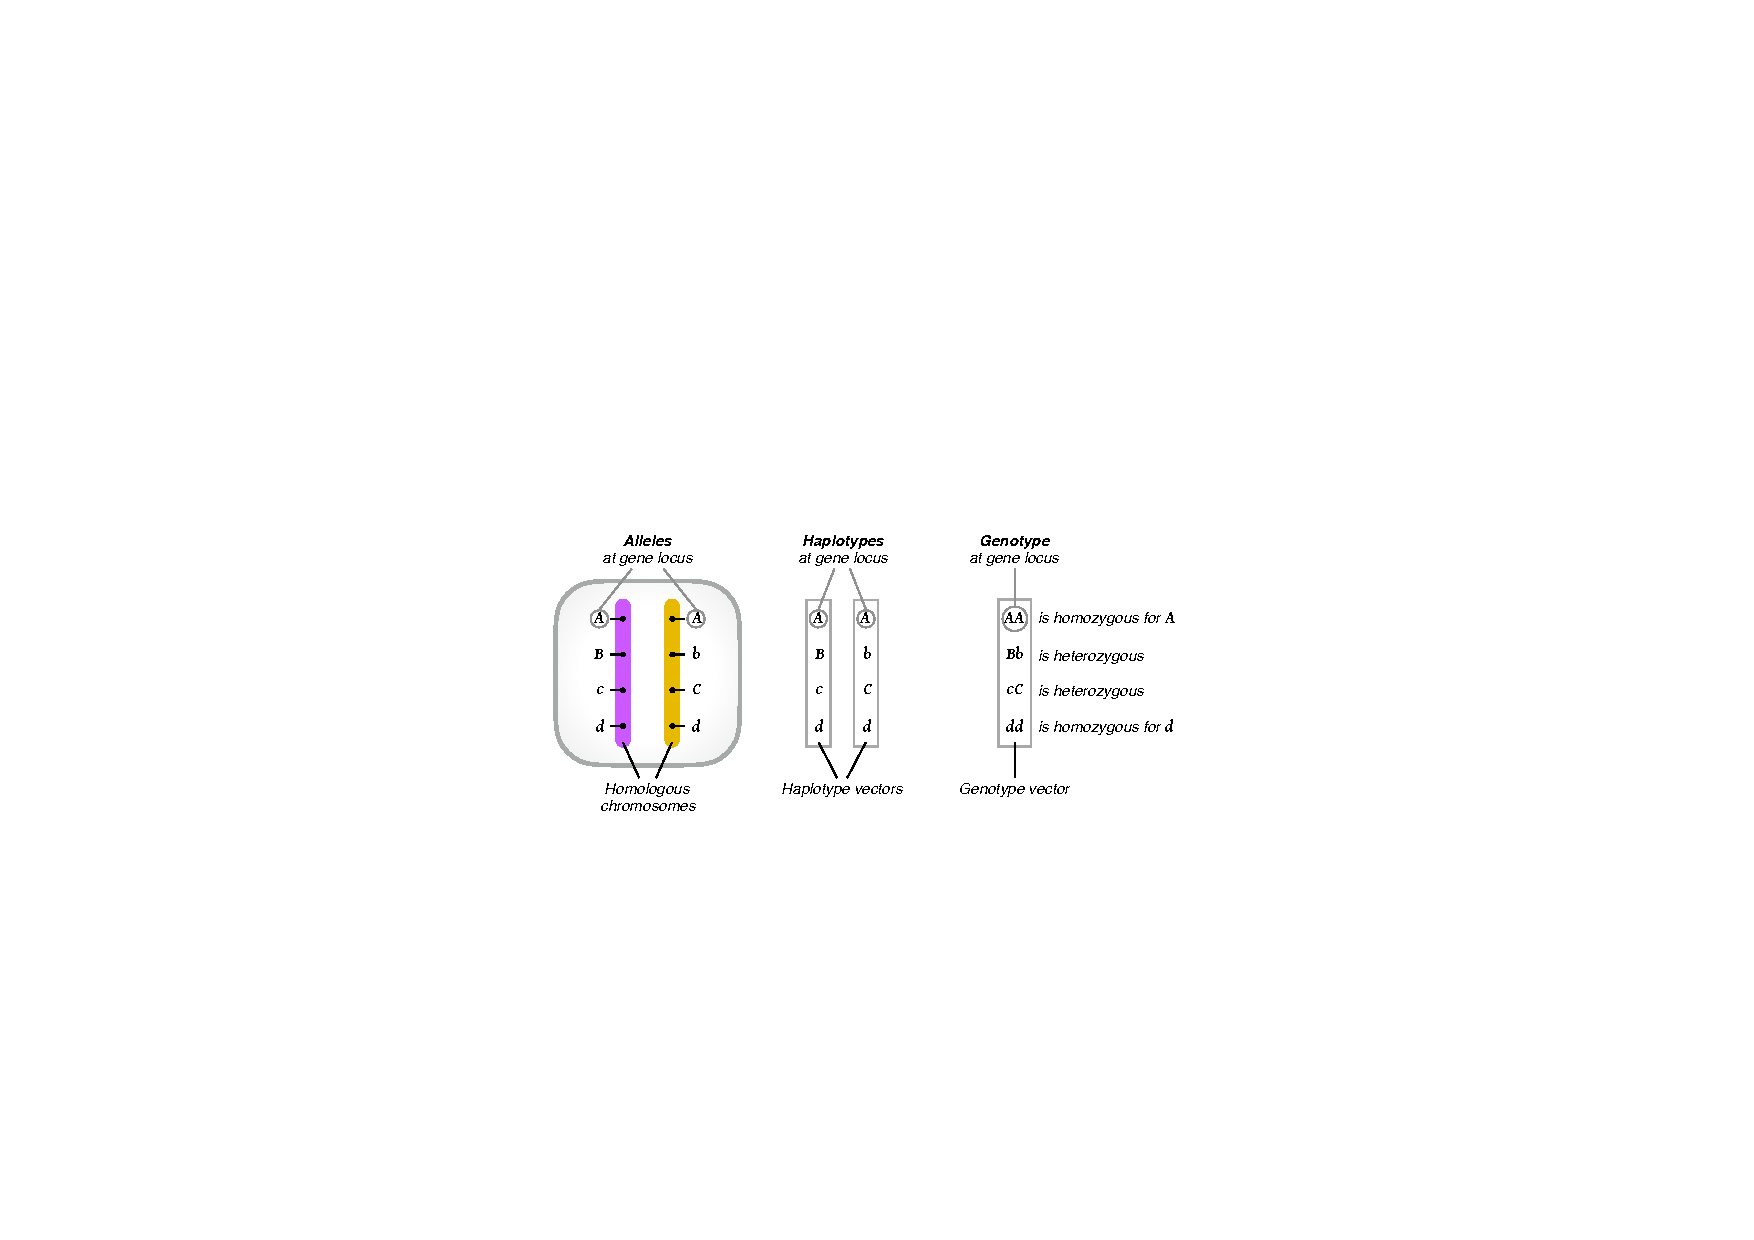
\includegraphics[width=0.8\textwidth]{./img/ch1/info_types}
\Caption{Alleles, haplotypes, and genotypes}
{A pair of homologous chromosomes is shown (\emph{left}) on which \n{4} gene loci are highlighted; labelled as $A$, $B$, $C$, and $D$.
Maternal and paternal chromosomes are shown in \emph{purple} and \emph{yellow} (arbitrarily coloured).
Each gene may have \n{2} allelic states (in this example), distinguished by capitalisation of the label.
Each chromosome has a corresponding haplotype at each locus (\emph{middle}).
Genotypes do not distinguish chromosomes and are represented as the sum of allelic information inherited from both parents (\emph{right}).
Note that the term \emph{haplotype} may refer to the allelic state observed at a single nucleotide or a set of alleles observed along a chromosome.
Likewise, the term \emph{genotype} may refer to the allelic dosage at a single site or a vector of observed genotypic information.}
{fig:info_types}
% \vspace{-5pt}
% \hrulefill%
\end{figure}

%

Note that the meaning of the word \emph{gene} has changed over time \citep[\eg see][]{slack2014genes}.
Historically, before the molecular basis of DNA was discovered, a gene was informally defined as the smallest unit of heredity, referring to the determinant of a characteristic that is transmitted from parent to offspring.
% This definition is convenient to mathematically describe the process of genetic inheritance and shall therefore be used in the remainder of this thesis.
A gene may be observed in different variant forms in the population, each distinguished as an \emph{allele}.
Further, a \emph{locus} (plural~\emph{loci}) refers to the physical location of a gene on a chromosome, but may also be used in reference to the position of a single nucleotide (or \emph{site}) in the genome.
When a set of sites on a single chromosome is considered, \ie the alleles observed at \n{1} or more loci, the term \emph{haplotype} is used.
While \n{1} \emph{maternal} and \n{1} \emph{paternal} haplotype can be distinguished in a diploid individual, its \emph{genotype} refers to the sum of the inherited genetic information at \n{1} or more loci in the \n{2} chromosomes.
An individual can be \emph{homozygous} for a particular allele at a given site if the allele is identical in both parents, or \emph{heterozygous} if the inherited alleles differ.
This terminology is further clarified in \cpref{fig:info_types}.

The following sections describe the main processes which generate genetic variation and, thereby, phenotypic variation in a population; namely mutation (\ccref{sec:mutation}) and recombination (\ccref{sec:recombination}).


%
\subsection{Mutation}
\label{sec:mutation}
%

A mutation constitutes a lasting change in the genetic sequence, \eg caused by imperfect \gls{dna} replication during cell division or due to errors in the \gls{dna} repair process.
The change may initially be only present in \n{1} cell, but it is passed on to daughter cells in the course of successive cell divisions (\emph{mitosis}).
If mutations occur in the germline, \ie germ cells which give rise to haploid \emph{gametes} (sperm and egg cells) during \emph{meiosis}, the nucleotide sequence is permanently altered in all cells of the progeny.
If a mutation has no effect on the reproductive success of an individual, it is said to be selectively \emph{neutral}; otherwise, a mutation may lead to a selective advantage or disadvantage, \eg due to a \emph{beneficial} or \emph{deleterious} effect on the phenotype, respectively.
In humans, the average rate of mutation per site and per generation, denoted by $\mu$, is typically as low as \n{1} mutation event every 100~million base~pairs.
More specifically, recent studies suggest a mutation rate of ${\mu\approx\val{1.1e-8}}$ \citep{Roach:2010ef} or ${\mu\approx\val{1.2e-8}}$ \citep{Scally:2012fe}.

Mutations generate the genetic variation that is observable in a population; several classes of genetic \emph{variants} can be distinguished \citep[\eg see][]{Frazer:2009hg}.
A change at a single position on the chromosome results from a \emph{substitution} of \n{1} base for another, which in sample data is observed as a \gls{snp}.
Nucleotides may be added to or removed from the sequence, due to \emph{insertions} or \emph{deletions} respectively, commonly referred to as \emph{indels}.
Larger changes to the chromosomal structure may also be distinguished.
This thesis is mainly concerned with genetic variation observed at individual positions in the genome.
In the following, the term ``mutation'' is used in reference to substitutions at single loci that result in observable \glspl{snp} in sample data.
It is further assumed that \gls{snp} loci are \emph{biallelic}, \ie there are \n{2} alleles that segregate in a population (sample) at a given locus; this is the case for the vast majority of \glspl{snp}.


%
\subsection{Recombination}
\label{sec:recombination}
%

Recombination refers to the reorganisation of alleles during meiosis in sexually reproducing organisms, which is facilitated through the physical exchange of genetic material between maternal and paternal chromosomes, such that new combinations of alleles are generated and transmitted to the offspring.
\N{2} main mechanisms of recombination can be distinguished.
\begin{description}
	\item[\textbf{Chromosomal crossover}] refers to the overlap of \n{2} chromatids (replicated maternal and paternal chromosomes) with subsequent, mutual exchange of homologous \gls{dna} segments.
	\item[\textbf{Gene conversion}] is a non-reciprocal exchange of genetic material.
	The \gls{dna} sequence at a section in \n{1} of the chromatids is replaced by a copy of the sequence on the other chromatid, resulting in the loss of its original sequence.
\end{description}
\Correct{Here, chromosomal crossover is implied as the acting mechanism of recombination, whereas gene conversion is not considered in this thesis.
In the following, the term \emph{recombination} therefore refers to crossover events between two homologous chromosomes.}

%
%!TEX root = ../../main.tex


\begin{figure}[!htb]
\centering
%\hrulefill \\
%\vspace{5pt}
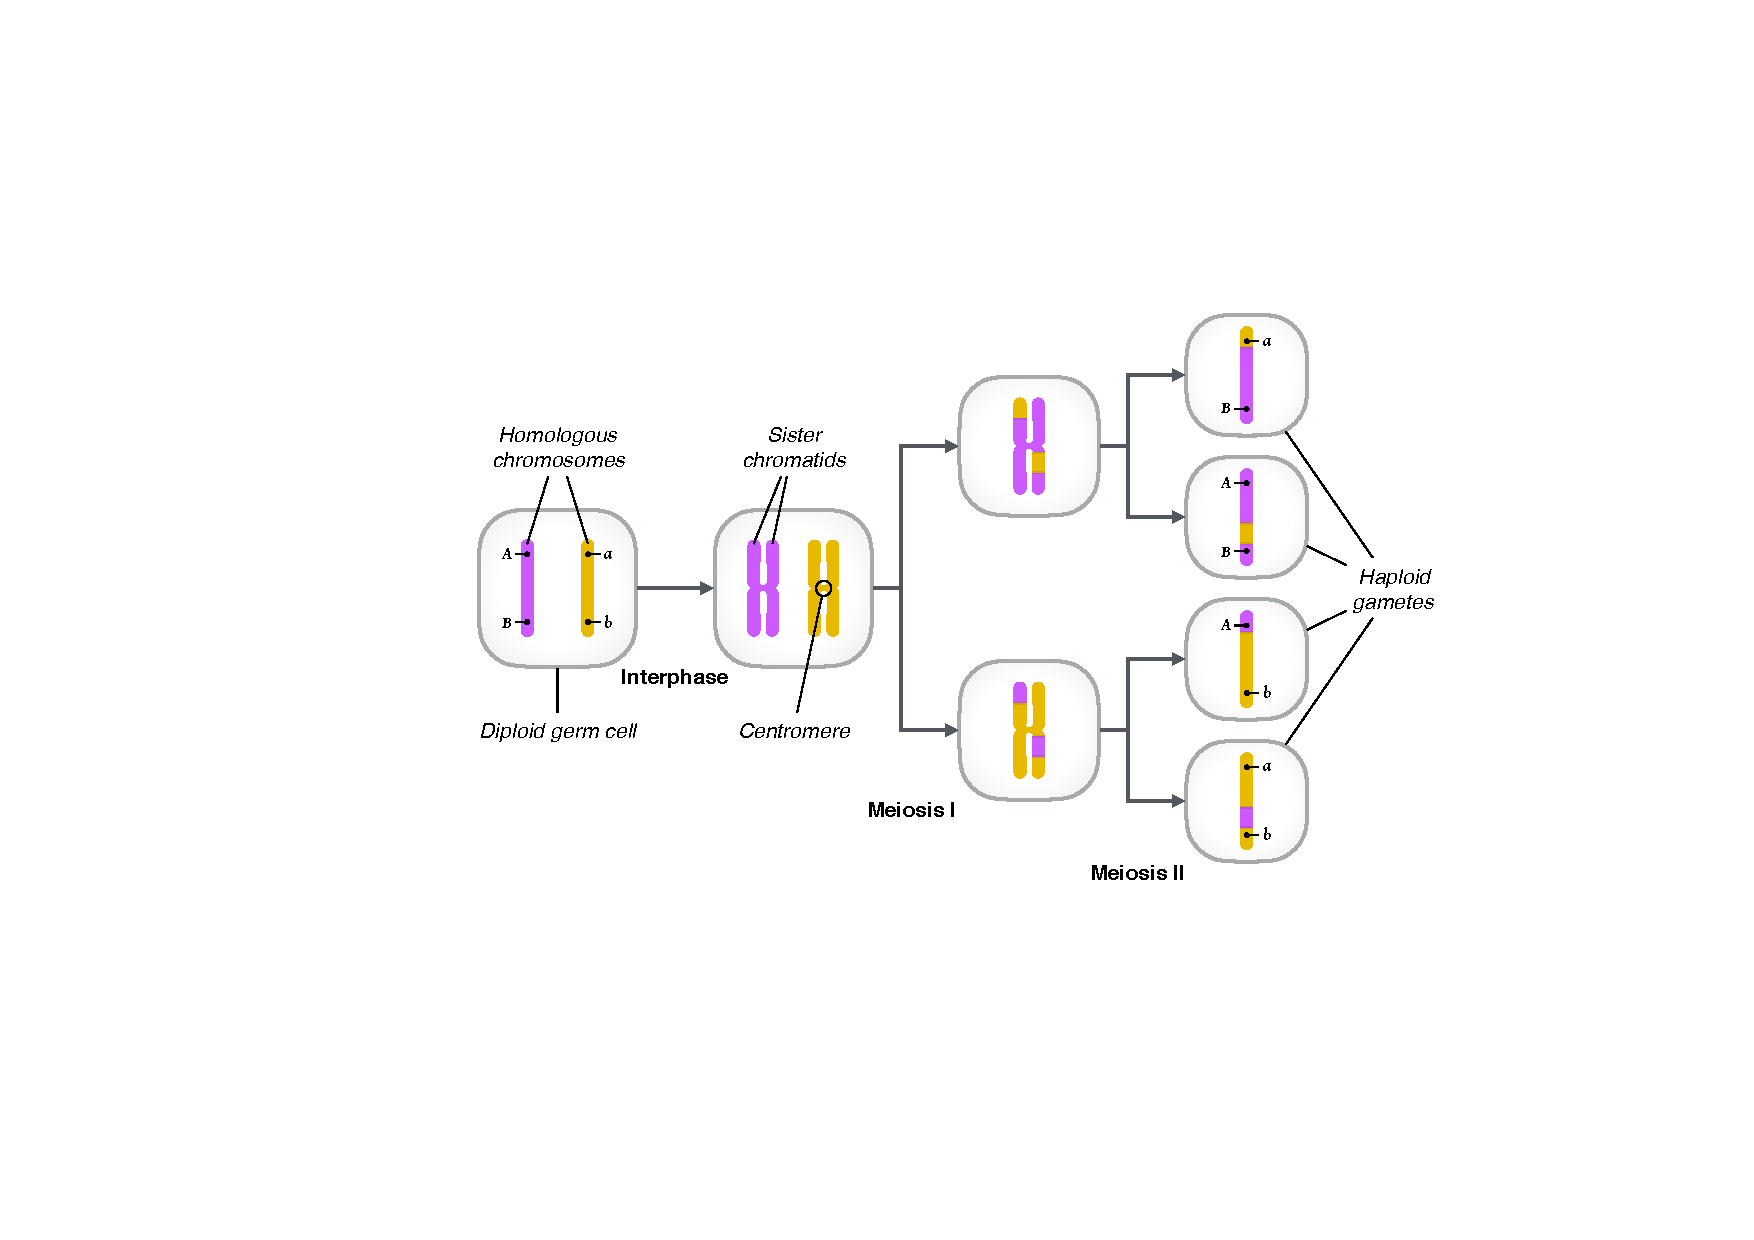
\includegraphics[width=0.9\textwidth]{./img/ch1/info_meiosis}
\Caption{Illustration of recombination during meiosis}
{\N{1} pair of homologous chromosomes is shown at the beginning of the meiotic cell cycle (\emph{left}).
Maternal and paternal chromosomes are shown in \emph{purple} and \emph{yellow} (arbitrarily coloured).
The allelic configuration at \n{2} sites is indicated on both chromosomes; $(A,B)$ and $(a,b)$.
\Gls{dna} sequences are replicated during the \emph{Interphase} of meiosis, where each chromosome forms \n{2} identical \emph{sister chromatids} which are held together at the \emph{centromere}.
Homologous chromosomes are paired at the beginning of the first cell division (\emph{Meiosis~I}), during which sequence segments are exchanged between chromatids through crossover.
In the second cell division (\emph{Meiosis~II}), the \n{4} chromatids are then separated into haploid gametes (\emph{right}).}
{fig:info_meiosis}
% \vspace{-5pt}
% \hrulefill%
\end{figure}

%

Consider the haplotypes at \n{2} loci in an individual which is heterozygous for both the alleles at these loci.
Given gene locus $\mathcal{A}$ with alleles $A$~and~$a$, and locus $\mathcal{B}$ with alleles $B$~and~$b$, the observed allelic configurations are $(A,B)$ on \n{1} of the chromosomes and $(a,b)$ on the other.
If no recombination occurs between the \n{2} loci during meiosis, the resulting gametes retain the configuration as present in the parental chromosomes; \ie the offspring may either receive $(A,B)$ or $(a,b)$.
In presence of recombination, in particular if the number of recombination events between loci is odd, the association between the \n{2} loci is broken such that either $(A,b)$ or $(a,B)$ are transmitted to the offspring.
An even number of recombination events between the \n{2} loci reverts the configuration of alleles.
Both cases (odd and even numbers of recombination events) are illustrated in \cpref{fig:info_meiosis}.


%
\subsubsection{Genetic linkage}
\label{sec:linkage}
%

A direct consequence of meiotic recombination is the phenomenon of genetic linkage, which was discovered by \citet{morgan1911} in experiments on \textsl{Drosophila}.
Linkage describes the concept that genetic markers located in close proximity to each other are less likely to be separated by recombination during meiosis.
This concept was further developed by \citet{sturtevant1913}, who proposed that the frequency of recombination between a set of markers can be used to determine the linear order of genes on a chromosome.
It was this idea that paved the way for the development of molecular and statistical methods for the purpose of \emph{linkage analysis}, through which it became possible, for example, to detect the chromosomal location of genetic variants implicated in human disease.

The earliest models of recombination go back to \citet{haldane1919}, who defined \emph{genetic distance}
as the expected number of recombination events per meiosis between \n{2} loci.
The unit of genetic distance is called a \emph{Morgan}.
However, it is more common to express genetic distance in units of \gls{cM}, where ${1~\text{Morgan}}$ is equal to ${100~\text{cM}}$.
For example, if \n{2} loci sit 1~\gls{cM} apart on a chromosome, the expected number of recombination events between them is $0.01$ per generation, meaning that the \n{2} loci are separated once every \n{100} meioses on average.
In humans, a distance of 1~\gls{cM} corresponds to about 1~million base pairs; \ie 1~\gls{Mb}.
The genetic distance translates into the rate of recombination, here denoted by $\rho$.
The human genome exhibits an average rate of ${\rho\approx\num{1e-08}}$ per site per generation.
However, the recombination rate varies among chromosomes and more so along the length of each chromosome.



%
\section{Models in population genetics}
\label{sec:popgen}
%

Over the last century, the field of population genetics has evolved from a mainly theoretical area of study into a more applied area of research.
More recently, the field has adapted to the exponential growth of available molecular data and continues to fill a niche in the computational sciences so as to be able to analyse the increasing amounts of data and to answer questions of biological as well as medical meaning.
This section outlines the statistical concepts on which many of the current analytical approaches are based.
Coalescent theory is of particular importance for the understanding of the statistical methods developed in this thesis, for which the Wright-Fisher model may serve as an introduction.

%
\subsection{Wright-Fisher model}
%

One of the most influential models in population genetics is the Wright-Fisher~model of reproduction \citep{Fisher1930,Wright1931}, which describes how gene frequencies evolve over time in a finite population.
Because the Wright-Fisher model is often implied in other statistical applications in population genetics, it is pertinent to explore its properties in greater detail.
In particular, the following describes the effects of ``random genetic drift'' in an idealised population.

%
%!TEX root = ../../main.tex


\begin{figure}[!htb]
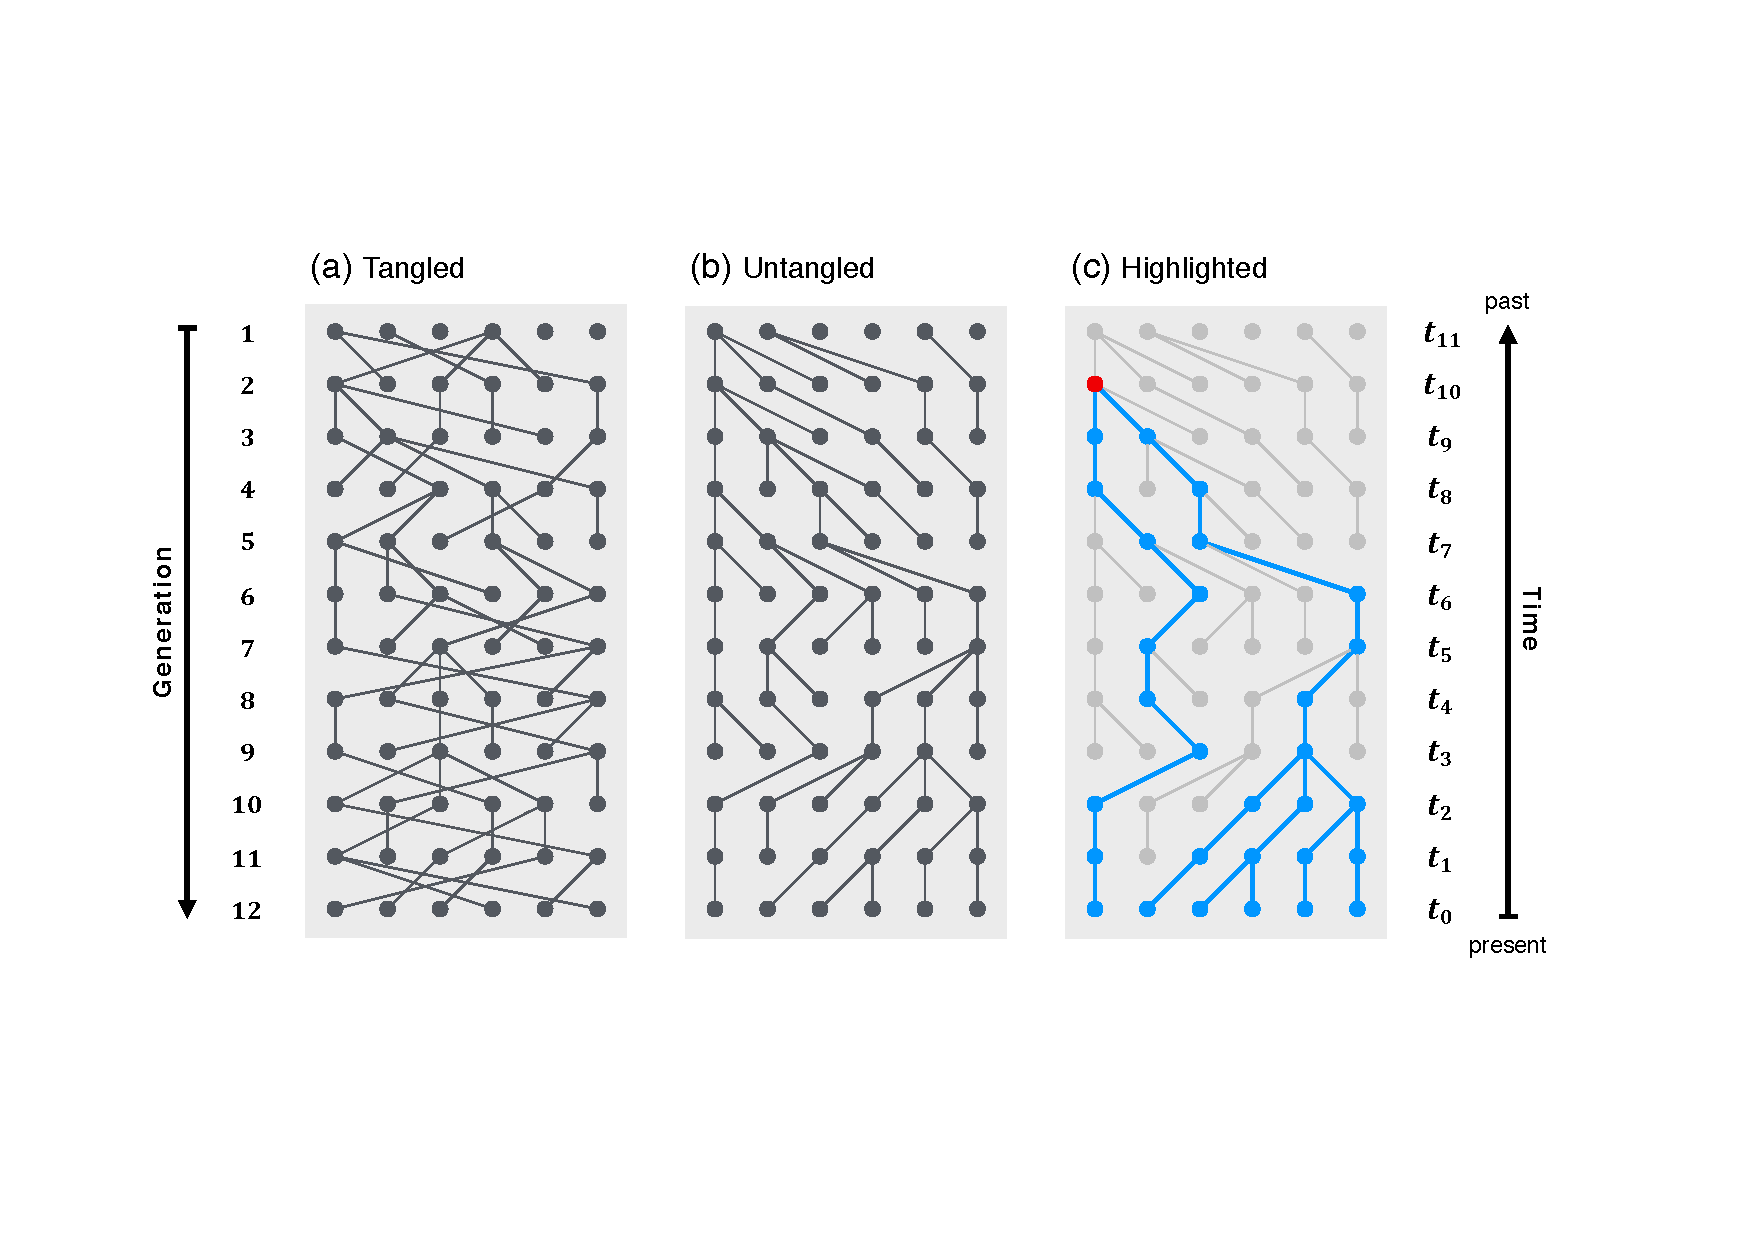
\includegraphics[width=\textwidth]{./img/ch1/info_wrightfisher}
\Caption{Example genealogy in a Wright-Fisher model}
{A population of size ${N=6}$ is shown in Panel~\textbf{(a)}, which is observed over 12 generations.
In the neutral Wright–Fisher model, \n{1} individual is chosen at random (with replacement) in each generation to produce offspring for the next generation, repeated $N$~times.
The genealogy of the population is more clearly seen after individuals have been sorted such that their lineages do not cross; see Panel~\textbf{(b)}.
Note that not every individual produces offspring, such that some lineages go extinct.
If this process is repeated over many generations (forward in time), it can be seen that all individuals in the present generation derive from a single individual in the past, which is indicated in Panel~\textbf{(c)}.
The ancestry of the present population (\emph{blue}) is traced back to a single ancestor (\emph{red}) at time ${t=10}$~generations ago.}
{fig:info_wrightfisher}
\end{figure}

%

In its simplest form, the Wright-Fisher model considers a gene locus at which \n{2} alleles, $A$~and~$a$, are observed; \ie the locus is \emph{biallelic}.
A population of $N$~haploid individuals is assumed, where $N$ remains constant in each generation.
All individuals die at the same time at which all individuals in the next generation are born; \ie time is measured in discrete, non-overlapping generations.
The effects of mutation or selection are ignored, such that alleles are \emph{neutral} and the probability of producing offspring is equal for each individual.
It follows that reproduction is considered as a random sampling process, in which the alleles that are transmitted into the next generation are drawn (with replacement) from the gene pool of the current population.
An example is illustrated in \cpref{fig:info_wrightfisher}.

Since each draw has only \n{2} possible outcomes, $A$~or~\Correct{$a$}, each generation is produced by a series of independent Bernoulli trials such that allele frequencies are binomially distributed.
Let $X_t$ denote the number of $A$ alleles in generation $t$.
Given ${X_t=i}$ allele copies (or individuals which carry the allele),
the probability of drawing the $A$ allele is equal to its frequency in the current generation, denoted by ${\pi_i = \rfrac{i}{N}}$.
The probability of observing ${X_{t+1}=j}$ copies in the next generation is
\begin{equation}\label{eq:WFprob}
	P(j \mid i) ~=~ {{N}\choose{j}} ~ \pi_i^j ~ (1 - \pi_i)^{N-j}
\end{equation}
for ${0 \leq i,j \leq N}$, and where ${\sum_{j=0}^{N} P(j \mid i) j = i}$.
From the binomial distribution follows that the expected number of alleles in the next generation can be expressed as
\begin{equation}\label{eq:WFexp}
	\mathbb{E}[X_{t+1} \mid X_{t}] ~=~ N \pi_i ~=~ N \frac{X_t}{N} ~=~ X_t
\end{equation}
and the variance is given by
\begin{equation}\label{eq:WFvar}
	\operatorname{Var}[X_{t+1} \mid X_{t}] ~=~ N \pi_i (1 - \pi_i) ~=~ X_t \Big( 1 - \frac{X_t}{N} \Big)
	\ \text{.}
\end{equation}

\Cref{eq:WFexp} implies that ${\mathbb{E}[X_t] = \mathbb{E}[X_{t-1}]}$ and thereby ${\mathbb{E}[X_t] = \mathbb{E}[X_0]}$; \ie the expected number of alleles in each generation is (on average) equal to the initial allele count.
This result is reminiscent of the Hardy-Weinberg principle \citep{Hardy:1908wx,Weinberg:1908tr}, which states that the relative allele frequency remains constant in each generation if mating is random, but in which the population size is assumed to be infinite.
However, due to the behaviour of a stochastic process in a finite population, the number of allele copies may eventually \emph{drift} to $0$~or~$N$, even in a single generation.
Several examples of how the allele frequency may change in populations of different sizes are shown in \cpref{fig:wfsim}.

%
%!TEX root = ../../main.tex


\begin{figure}[!htb]
\centering
%\hrulefill \\
%\vspace{5pt}
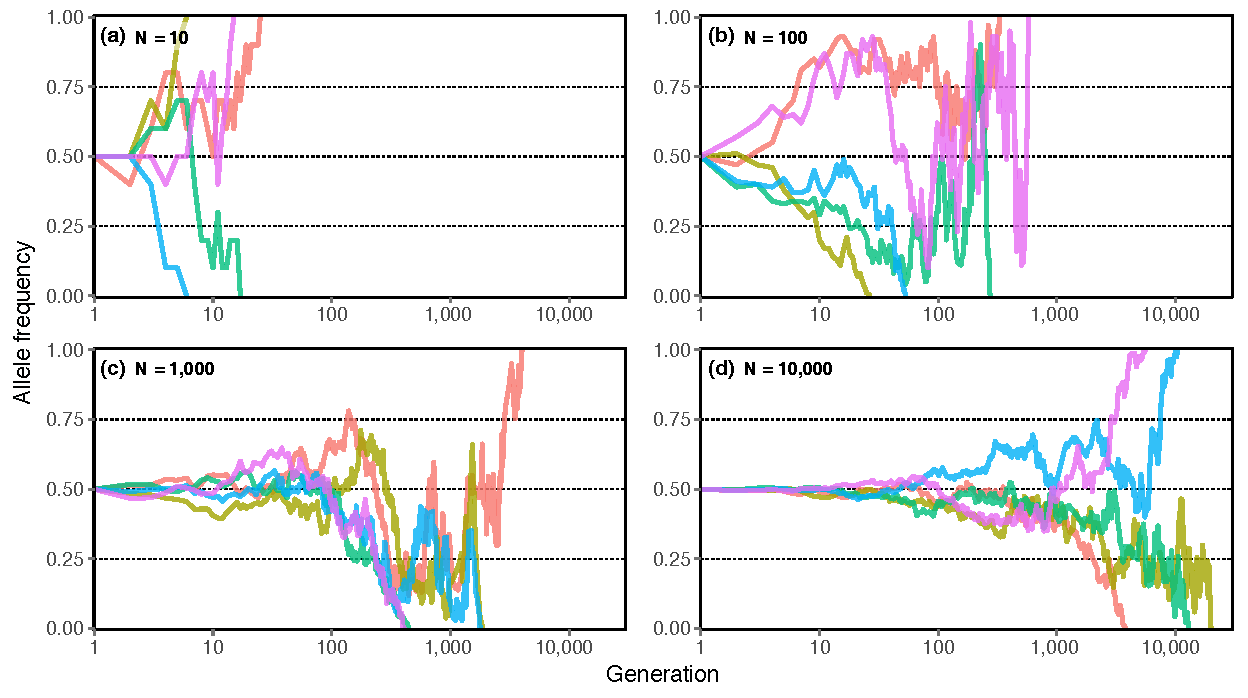
\includegraphics[width=\textwidth]{./img/ch1/wfsim}
\Caption{Allele frequency changes over time simulated under the Wright-Fisher model}
{A haploid population was simulated under \n{4} different constant values of population size, $N$, as indicated in each panel.
The change in allele frequency is shown by generation.
For each value of $N$, \n{5} replicate simulations were conducted (distinguished by colour).
Note that the allele frequency does not change after it has reached 0~or~1; \ie the allele is said to have become \emph{fixed} in the population.}
{fig:wfsim}
% \vspace{-5pt}
% \hrulefill%
\end{figure}

%

Because the frequency of an allele in a particular generation only depends on the frequency distribution in the previous generation, it follows from this property that the reproductive process is itself a Markov chain, with transition probabilities as described by \cref{eq:WFprob} and a state space in $\{0,\ldots,N\}$.
The states $0$ and $N$ are absorbing, which means that if the population consists of ${X_t=0}$ or ${X_t=N}$ alleles, it remains so in all future generations.
A consequence of this Markov process is that an allele will either go extinct or reach \emph{fixation} \citep[\eg, see][]{ewens2012}.
Let the time until either of the \n{2} alleles has reached fixation be denoted by $T$.
From \cref{eq:WFexp} follows that the probability that an allele reaches fixation is
\begin{equation}
	P(X_T \in \{0,N\}) = \frac{X_0}{N}
\end{equation}
which means that the probability of a given allele reaching fixation is equal to its initial frequency.

Without the introduction of new alleles through mutation, the Wright-Fisher model predicts that genetic variation is inevitably lost over time, due to random drift resulting from sampling error in a finite population. \label{ref:mutgendiv}
Hence, an important extension of the Wright-Fisher model is the incorporation of mutations.
Suppose that allele~$A$ mutates into allele~$a$ with rate~$\mu_A$, and $a$~into~$A$ with rate~$\mu_a$.
The transition probability given in \cref{eq:WFprob} still holds, but allele frequency can be expressed such that $\pi_i$ is dependent on mutation rate, namely
\begin{equation}
	\pi_i ~=~ \frac{i}{N} ~ (1 - \mu_A) ~+~ \Big( 1 - \frac{i}{N} \Big) ~ \mu_a \ .
\end{equation}
If ${\mu_A, \mu_a > 0}$, then transitions from any state into any other state remain possible in each generation and permanent \Correct{extinction or} fixation is avoided.
Note that in a population in which the effects of mutation and genetic drift are in statistical equilibrium allele frequencies are expected to follow the Hardy-Weinberg principle; \ie the population is in \gls{hwe}.


%
\subsection{Coalescent theory}
\label{sec:coalescent}
%


The coalescent is arguably the most frequently employed genealogical method in population genetics.
The concept and the statistical properties of the coalescent were first described by \citet{Kingman:1982x,Kingman:1982gu,Kingman:1982uj} and it is therefore often referred to as ``Kingman's~coalescent''.
The term ``$n$-coalescent'' is also frequently used to emphasise the importance of the sample size, $n$, in the genealogical process within a much larger population.
The coalescent, at its core, is a collection of stochastic models which provide the means to generate predictions about population dynamics under a variety of models of genetic variation and demography \citep{wakeley2008}.
Note that the term ``prediction'' may sound odd given that the coalescent looks backward in time to reconstruct a possible genealogy given a set of population parameters.
The coalescent is often used to simulate the ancestry of a sample, from which particular model parameters can be inferred, for example, on basis of biological observations.
The first computational algorithm for simulations under the coalescent (named ``\texttt{ms}'') was devised by \citet{Hudson:1990vob}.
Over the past decades, coalescent theory has grown extensively.
Hence, this section provides only a summary of the basic properties of the coalescent as relevant for this thesis.
For a more thorough presentation of the subject see, for example, \citet{Fu:1999fj}, \citet{neuhauser2001}, \citet{nordborg2001coalescent}, \citet{hein2004gene}, and \citet{wakeley2008}.


In contrast to the Wright-Fisher model, as well as other approaches which model the genealogical history of a population forward in time, the coalescent process reconstructs the genealogy of a sample by tracing the ancestry of individuals (or genes) backward in time.
Ancestral relationships between individuals are represented as lineages in a genealogical tree.
In each generation, each individual independently chooses \n{1} ancestor at random.
If \n{2} individuals choose the same ancestor by chance, their lineages are joined; \ie they \emph{coalesce}.
The time at which \n{2} lineages join is referred to as a \emph{coalescent~event}.
This process is repeated until only \n{1} lineage is left, which belongs to the \gls{mrca} of the sample.

%
%!TEX root = ../../main.tex


\begin{figure}[!htb]
\centering
%\hrulefill \\
%\vspace{5pt}
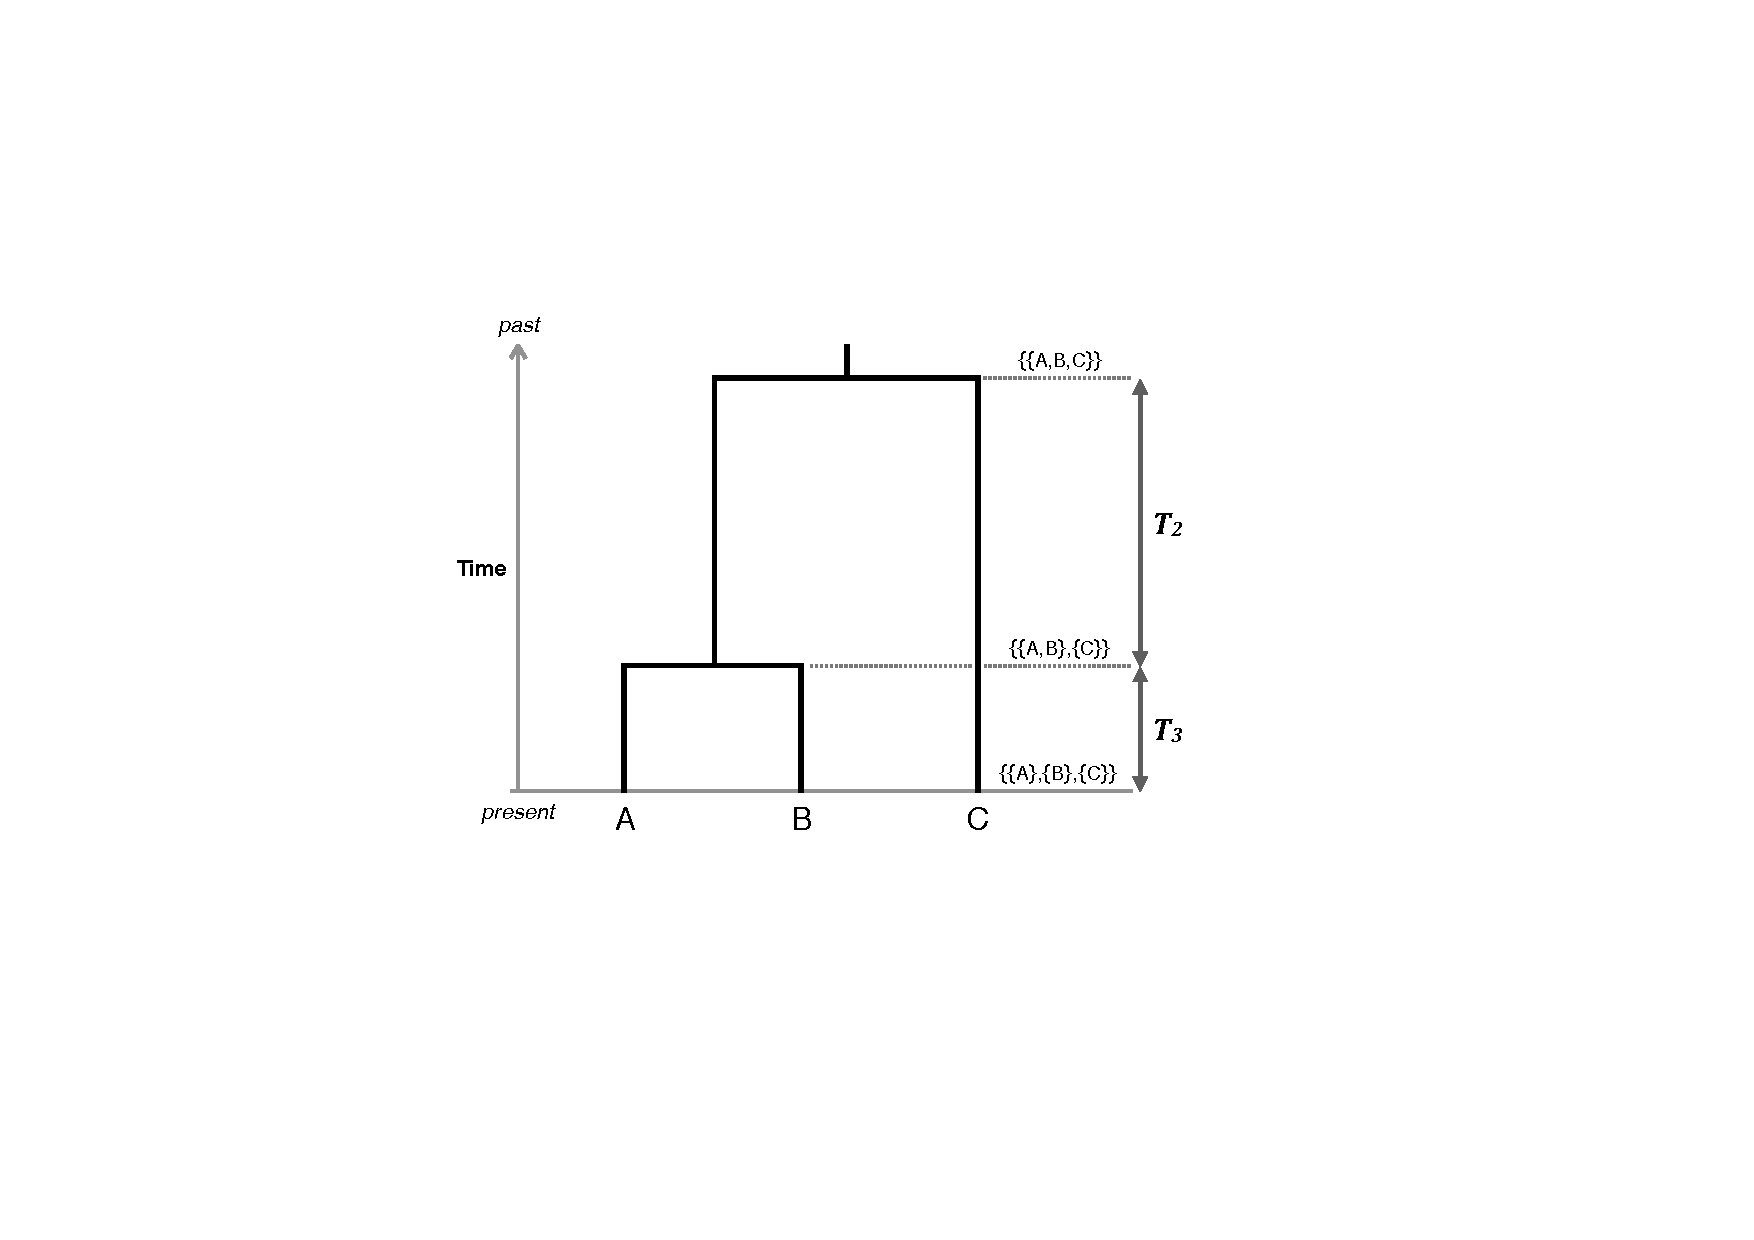
\includegraphics[width=0.7\textwidth]{./img/ch1/info_coalescent}
\Caption{Topology of a genealogical tree in the coalescent}
{The genealogical relationship of \n{3} haploid individuals is shown, $A$, $B$, and $C$, which represent separate lineages at present, but where $A$~and~$B$ are the first to coalesce (back in time).
The waiting time between successive coalescent events is denoted by \Correct{$T_j$}, where \Correct{$j$} is the number of ancestral lineages at a given time interval, which changes from \Correct{$j$} to \Correct{${j-1}$} at coalescence.
Figure modified from \citet{nordborg2001coalescent}.}
{fig:info_coalescent}
% \vspace{-5pt}
% \hrulefill%
\end{figure}

%

The history of a sample is reflected in its genealogy and can be described in terms of the topology of the tree and the lengths of the connecting branches.
The branch length corresponds to the time interval between \n{2} successive coalescent events, which is of central interest in describing the coalescent process.
Let this waiting time be denoted by \Correct{$T_j$}, where \Correct{$j$} corresponds to the number of distinct lineages during the time interval, which changes from \Correct{$j$} to \Correct{${j-1}$} at coalescence.
An example of a simple genealogical tree is shown in \cpref{fig:info_coalescent}, in which the waiting times between coalescent events are indicated.
In the following, the concept of the standard coalescent is described by assuming a haploid population of constant size, $N$, in which the effects of mutation, selection, recombination, or other biological processes are not involved.

For now, consider a sample of ${n=2}$ individuals taken at the present time, which are followed back in time until the first coalescent event.
Since there are $N$ possible ancestors, the probability that a particular ancestor is chosen by \n{1} of the individuals is equal to $N^{-1}$.
The probability that \n{2} individuals choose the same ancestor independently is $N^{-2}$.
Hence, the probability that any of the possible ancestors is chosen by \n{2} individuals is equal to ${N \times N^{-2} = N^{-1}}$, and the probability that none is chosen is ${1 - N^{-1}}$.
To arrive at the probability that \n{2} lineages coalesce $t>0$ generations back in time, it is implied that they do not choose the same ancestor in previous generations.
Because generations are independent, the probability that the \n{2} lineages are distinct over $t-1$~generations is
\begin{equation}
	P(T_2 \geq t \mid N) ~=~ \Big( 1 - \frac{1}{N} \Big)^{t-1}
	\ \text{.} \CorrectLabel
\end{equation}
Therefore, the probability that \n{2} lineages coalesce $t$ generations back in time is geometrically distributed with rate $N^{-1}$, such that
\begin{equation}\label{eq:coalprob}
	P(T_2 = t \mid N) ~=~ \Big( 1 - \frac{1}{N} \Big)^{t-1} ~ \frac{1}{N} \CorrectLabel
\end{equation}
which arises from the number of independent Bernoulli trials needed until the same ancestor is chosen by \n{2} lineages.
It follows from the geometric distribution that the expected number of generations up to and including the coalescent event is
\begin{equation}\label{eq:coal_2_exp}
	\mathbb{E}[T_2 \mid N] ~=~ \frac{1}{N^{-1}} ~=~ N
\end{equation}
and the variance is
\begin{equation}\label{eq:coal_2_var}
	\operatorname{Var}[T_2 \mid N] ~=~ \frac{1 - N^{-1}}{N^{-2}} ~=~ N^2 ~ \Big( 1 - \frac{1}{N} \Big)
	\ \text{.}
\end{equation}

A notable result is that the expected time to the first coalescent event is equal to the size of the population; see \cref{eq:coal_2_exp}.
It is therefore convenient to scale time in units of $N$~generations, namely
\begin{equation}\label{eq:timescale}
	\tau ~=~ \frac{t}{N}
\end{equation}
where the time, $\tau$, is continuous (as opposed to time measured in distinct generations) and referred to as the \emph{population-scaled} time.
The probability that a pair of lineages remains distinct during a given time interval is given below, and can now be approximated using the exponential distribution if the population size is sufficiently large, \ie as $N$ tends to infinity;
\begin{equation}\label{eq:coal_2_dont}
	P(T_2 > \tau \mid N)
	~=~ \Bigg( 1 - \frac{1}{N} \Bigg)^{\lfloor N \tau \rfloor}
	\quad \xrightarrow{~ N~\rightarrow~\infty ~} \quad
	\euler{-\tau}
\end{equation}
where ${\lfloor N \tau \rfloor}$ is the largest integer that does not exceed ${N \tau}$ \citep[\eg, see][]{nordborg2001coalescent}.

The above can now be extended to consider $n$~lineages, which in the previous generation may have $n$ distinct ancestral lineages if no coalescent event has occurred, or ${n-1}$ otherwise.
The probability of no coalescence at a given time can be derived as follows.
Let the first lineage choose among $N$~ancestors with probability ${\rfrac{N}{N} = 1}$, the second lineage then chooses among the remaining ${N-1}$ ancestors with probability ${\rfrac{(N-1)}{N}}$, the third chooses among ${N-2}$ ancestors with probability ${\rfrac{(N-2)}{N}}$, and so on; \ie
\begin{equation*}
	\Big(\frac{N}{N}\Big) ~ \Big(\frac{N-1}{N}\Big) ~ \Big(\frac{N-2}{N}\Big) ~ \cdots ~ \Big(\frac{N-(n-1)}{N}\Big)
\end{equation*}
which is equal to
\begin{equation}\label{eq:coal_n_dont}
	\prod_{k=0}^{n-1} \frac{N-k}{N}
	~=~ \prod_{k=1}^{n-1} \Big( 1 - \frac{k}{N} \Big)
	~=~ 1 - {n \choose 2} \frac{1}{N} ~+~ \mathcal{O}\Big( \frac{1}{N^{2}} \Big)
\end{equation}
where the binomial coefficient, ${{n \choose 2} = \sum_{k=1}^{n-1}k}$, corresponds to the number of possible pairs.
Similarly, the probability that any \n{2} of the $n$~lineages coalesce at a given time implies that the remaining lineages do not coalesce, therefore
\begin{equation}\label{eq:coal_n_do}
\begin{split}
	P(T_n = \tau \mid N)
	& ~=~ {n \choose 2} \frac{1}{N} ~\times~ \Big(1-\frac{1}{N}\Big) ~ \Big(1-\frac{2}{N}\Big) ~ \cdots ~ \Big(1-\frac{n-2}{N}\Big) \\
	& ~=~ {n \choose 2} \frac{1}{N} ~\times~ \prod_{k=1}^{n-2} \Big( 1 - \frac{k}{N} \Big) \\
	& ~=~ {n \choose 2} \frac{1}{N} ~+~ \mathcal{O}\Big( \frac{1}{N^{2}} \Big)
	\ \text{.}
\end{split}
\end{equation}
Note that the term ${\mathcal{O}(N^{-2})}$ describes the limiting behaviour of \cref{eq:coal_n_dont,eq:coal_n_do} and captures all terms that decrease more rapidly than $\rfrac{1}{N}$ as $N$ tends to infinity.
Mathematically, ${\mathcal{O}(N^{-2})}$ corresponds to the \emph{diffusion} limit of the continuous process, which can be ignored if the population size is sufficiently large \citep[\eg, see][]{wakeley2008}.
By doing so, it is assumed that not more than \n{2} lineages coalesce at a given time and that the resulting tree has a binary topology.
In the limit, and if ${n \ll N}$, the probability of a coalescent event at a given time is
\begin{equation}\label{eq:coal_approx}
	P(T_n = \tau \mid N) ~\approx~ {n \choose 2} \frac{1}{N}
\end{equation}
and, as before, the waiting time can be approximated in terms of the exponential distribution as given below.
\begin{equation}\label{eq:coal_n_approx}
	P(T_n > \tau \mid N)
	~\approx~ \Bigg( 1 - {n \choose 2} \frac{1}{N} \Bigg)^{\lfloor N \tau \rfloor}
	\quad \xrightarrow{~ N~\rightarrow~\infty ~} \quad
	\euler{-{n \choose 2}\tau}
\end{equation}
Thus, in the continuous-time coalescent, the approximate waiting time between successive coalescent events, $T_n$, is exponentially distributed with rate ${n \choose 2}$, from which follows that the expected value is
\begin{equation}\label{eq:coal_n_exp}
	\mathbb{E}[T_n] ~=~ \frac{1}{{n \choose 2}} ~=~ \frac{2}{n(n-1)}
\end{equation}
and the variance is
\begin{equation}\label{eq:coal_n_var}
	\operatorname{Var}[T_n] ~=~ \frac{1}{{n \choose 2}^2} ~=~ \frac{4}{n^2 (n-1)^2}
	\ .
\end{equation}

An important result of the coalescent is that an expectation for the \gls{tmrca} can be derived dependent on the population size.
Given the sum of branch lengths that need to be traced back to arrive at the \gls{mrca},
\begin{equation*}
	T_\text{MRCA} ~=~ T_N + T_{N-1} + \dots + T_2
\end{equation*}
the expected value can be expressed as
\begin{equation}\label{eq:coal_tmrca}
	\mathbb{E}[T_\text{MRCA} \mid N]
	~=~ \sum_{n = 2}^{N} \mathbb{E}[T_n]
	~=~ \sum_{n = 2}^{N} \frac{2}{n(n-1)}
	~=~ 2~\Big( 1 - \frac{1}{N} \Big)
	\ \text{.}
\end{equation}
Therefore, ${\mathbb{E}[T_\text{MRCA}] \approx 2}$ as ${N\rightarrow\infty}$, which implies that on average the number of generations until the entire sample has coalesced into a single ancestral lineage is equal to about twice the population size.


%
\subsubsection{Effective population size}
%

Natural populations rarely adhere to the assumptions made by mathematical models.
One such example is the rather unrealistic assumption that the population size remains constant over time.
The rate at which coalescent events occur in the genealogy of a sample is conditional on the size of the population in each generation, which in reality is often highly variable.
Statistical models in population genetics may therefore resort to the concept of an effective population size, denoted by \Ne, which substitutes the census population size, $N$, to account for departures from model assumptions.
Note that the biological meaning and the mathematical definition of \Ne may vary depending on the properties of the biological system under consideration.
To account for variations in population size in the standard coalescent, \Ne can be defined as the \emph{variance effective size} and is estimated such that the coalescent process would result in the same shape of genetic variation as expected in a population of constant size.

Note that \Ne may differ from the census size of a population by several magnitudes.
For example, the human population currently counts several billion individuals globally, whereas the long-term, diploid effective size is commonly defined in the order of ${\Ne \approx \num{10000}}$, based on estimates from \gls{dna} polymorphism data \citep[\eg][]{Takahata:1993ko,Yu:2001wl}.

Suppose the size of a population is known at each generation back time, where $N_i$ denotes the census size in generation~$i$ over a period of $t$ discrete generations.
The effective size can be computed as
\begin{equation}
	\Ne ~=~ \frac{t}{ \sum_{i=1}^{t} \frac{1}{N_i} }
\end{equation}
which is the harmonic mean of $N_i$.
However, because past population sizes are typically difficult to assess, \Ne can be estimated from the genetic diversity observed in a population.
The measure of genetic diversity is dependent on the rate of mutation in the genome, which is described in the following section\label{ref:calceffpopsize}.
For consistency with the definitions provided so far, the following sections in this chapter keep $N$ to denote the population size, but this is substituted by \Ne in the remaining chapters.


%
\subsubsection{The coalescent with mutation}
\label{sec:coal_mutation}
%

Mutations are essential to generate genetic diversity and maintain genetic variation in a finite population.
The standard coalescent relies on the assumption that variant alleles are selectively neutral; \ie the effect of mutation is independent of the genealogical process.
As such, mutation events can be superimposed on the coalescent tree by placing mutations on all branches proportional to their length.
An example is illustrated in \cpref{fig:info_mutation}, in which several mutation events are shown to give rise to the variation observed in the \gls{dna} sequence of a sample.

%
%!TEX root = ../../main.tex


\begin{figure}[!htb]
\centering
%\hrulefill \\
%\vspace{5pt}
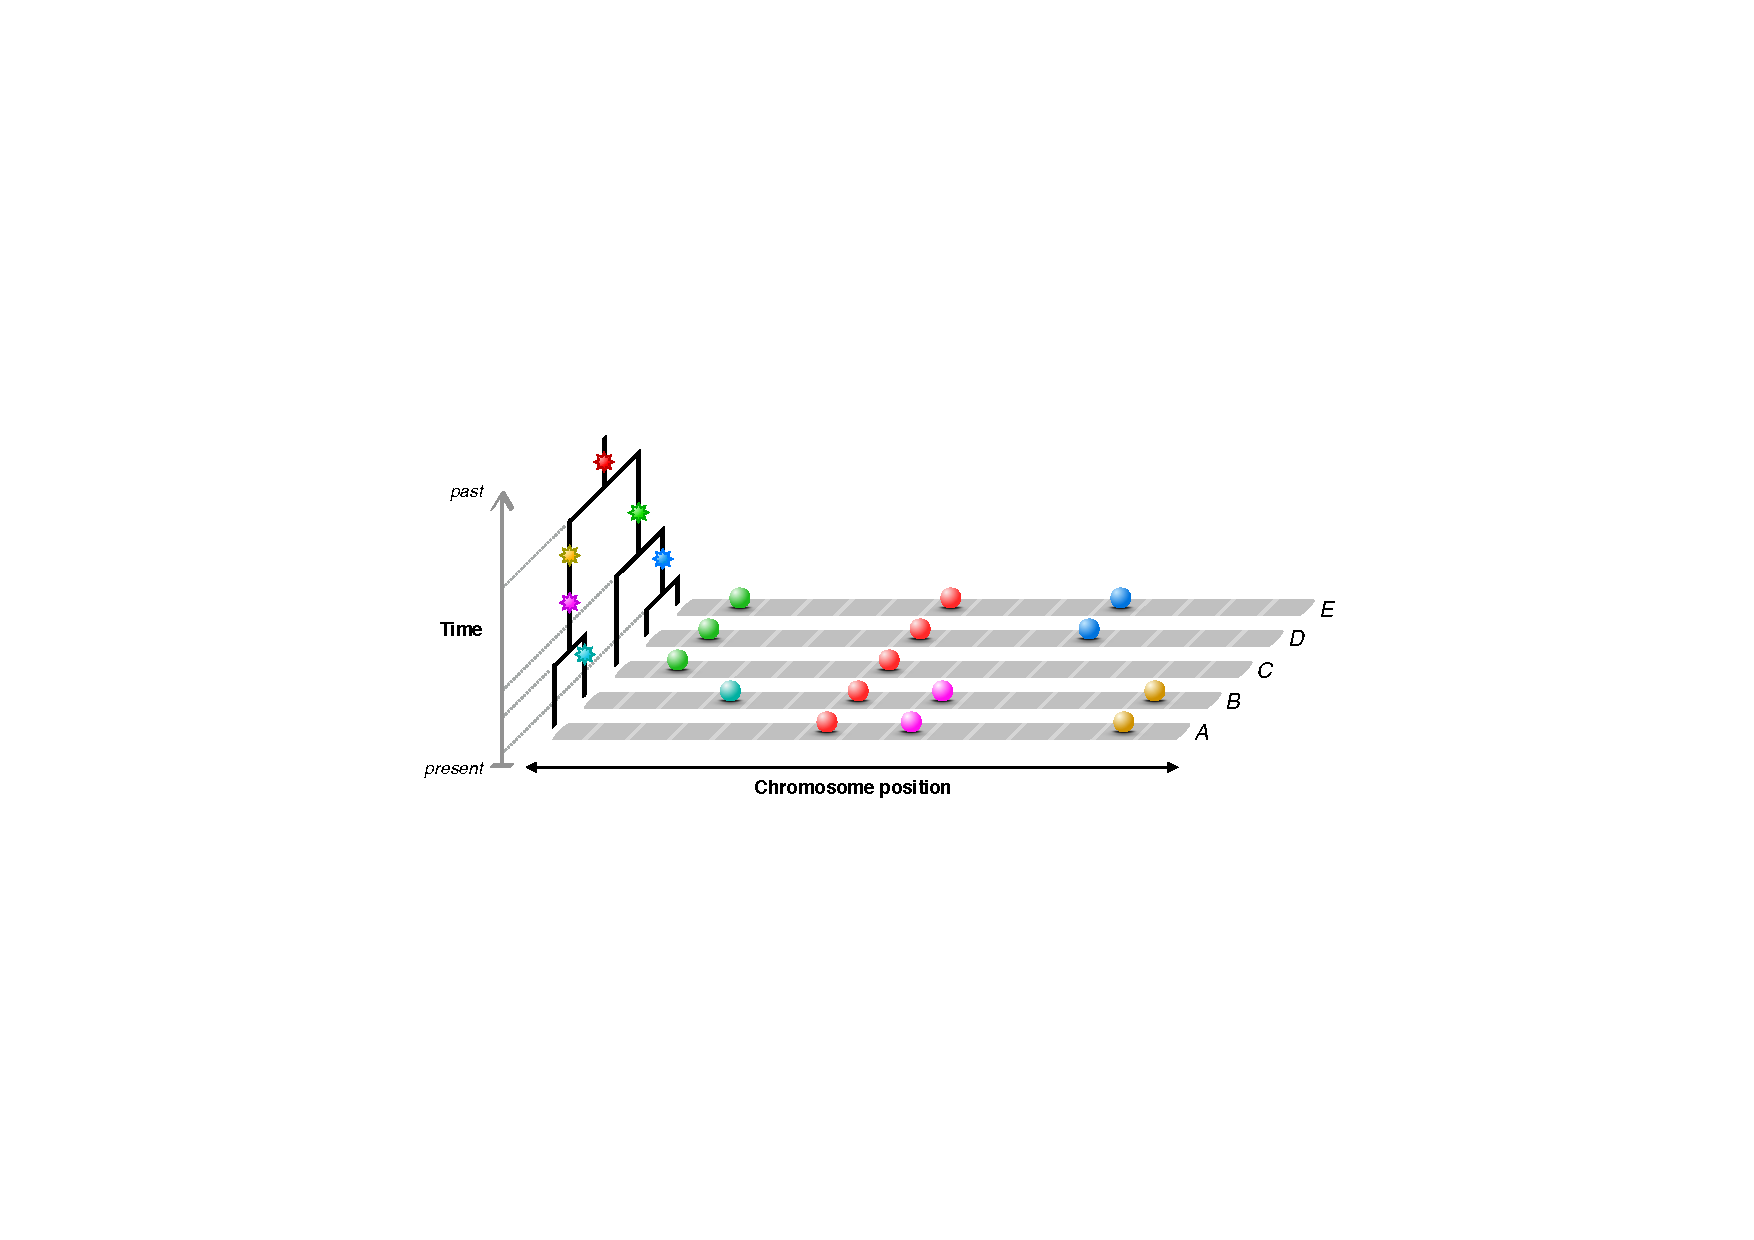
\includegraphics[width=\textwidth]{./img/ch1/info_mutation}
\Caption{Mutation events on a genealogical tree in the coalescent}
{The genealogy of a sample of \n{5} haploid individuals ($A-E$) is shown on the left.
The time of each coalescent event is indicated by a \emph{dotted} line.
Mutation events (\emph{stars}) are placed along the branches of the tree.
Each mutation event alters the allelic state at a random position on the chromosome, giving rise to a new allele, which is inherited by all descendants of the ancestral individual in which the mutation occurred.
Horizontal lanes (\emph{grey}) represent the chromosome sequence of the individuals, on which the derived alleles are depicted as \emph{marbles}; colours correspond to the mutation event from which the alleles derive.}
{fig:info_mutation}
% \vspace{-5pt}
% \hrulefill%
\end{figure}

%

Given a constant rate of mutation per site per generation, $\mu$, the expected number of mutations on a branch in the genealogical tree, \ie a lineage that is $t$~generations long, is ${t\mu}$.
If time is scaled in units of $N$~generations, see \ctref{eq:timescale}, the corresponding value is expressed by ${\tau N \mu}$, such that the rate of mutation per site per unit of time is equal to ${N \mu}$.
However, for historical reasons \citep[\eg, see][]{wakeley2008}, the population-scaled mutation rate is given by the compound parameter
\begin{equation}\label{eq:mutrate}
	\theta = 2 N \mu
\end{equation}
where $\theta$ is assumed to be constant in the limit ${N\rightarrow\infty}$.
Note that the factor of 2 relates to the formulation of the expected number of pairwise differences between \n{2} haploid sequences, which is equal to $\theta$ \citep{tajima1993}.
Thus, $\theta$ describes the amount of genetic diversity in a population.

Because mutations effectively count events that occur independently, the probability distribution of mutation is described by a Poisson process with rate parameter ${\rfrac{\theta}{2}}$ \citep{wakeley2008}.
It follows that the probability of observing $K$~mutations on a branch of length~$L$ is itself Poisson distributed with parameter ${\rfrac{\theta L}{2}}$;
\begin{equation}
	P(K = k \mid L) ~=~ \bigg( \frac{\theta L}{2} \bigg)^k ~ \frac{1}{k!} \euler{-\frac{\theta L}{2}}
\end{equation}
where ${L=t}$ if measured in discrete generations or ${L=N\tau}$ if measured on a continuous time scale.
It follows from the Poisson distribution that ${\mathbb{E}[K \mid L] ~=~ \operatorname{Var}[K \mid L] ~=~ \rfrac{\theta L}{2}}$.

Suppose that each mutation event creates a new allele and that each site can only mutate once in the history of the sample; such a setting is generally referred to as the infinite sites model \citep{Kimura:1969tn,Watterson:1975ur}.
Under this assumption, the number of segregating sites (or \emph{variant} sites) observed in sequence data in a sample of size~$n$, is equal to the sum of mutation events that occurred in the history of the sample.
The total branch length of the tree thereby determines the expected value of the number of segregating sites, denoted by $S_n$.
From the sum of all branch lengths, \ie
\begin{equation*}
	T_\text{total} ~=~ j T_j ~+~ (j-1) T_{j-1} ~+~ (j-2) T_{j-2} ~+~ \ldots ~+~ 2 T_2 \CorrectLabel
\end{equation*}
where \Correct{$j$} is the number of distinct lineages during a given time interval,
the expected value of the total branch length can be computed as
\begin{equation}
	\mathbb{E}[T_\text{total}]
	~=~ \sum_{i=2}^{n} i ~ \mathbb{E}[T_i]
	~=~ \sum_{i=2}^{n} i ~ \frac{2}{i(i-1)}
\end{equation}
where ${\mathbb{E}[T_i]}$ is given by \ctref{eq:coal_n_exp}.
From the above, the expected value of $S_n$ can be derived as follows.
\begin{equation}
	\mathbb{E}[S_n]
	~=~ \frac{\theta}{2} ~ \mathbb{E}[T_\text{total}]
	~=~ \frac{\theta}{2} \sum_{i=2}^{n} i ~ \frac{2}{i(i-1)}
	~=~ \theta \sum_{i=1}^{n-1} \frac{1}{i}
\end{equation}
By rearrangement, the following equation can be obtained;
\begin{equation}\label{eq:theta_w}
	\hat{\theta}_W = \frac{S_n}{\sum_{i=1}^{n-1} \frac{1}{i}}
\end{equation}
which is an unbiased estimator of the genetic diversity in \Correct{a} sample of sequence data; also known as Watterson's $\theta$ \citep{Watterson:1975ur}.
With regard to the calculation of the effective population size as described in the previous section (\pref{ref:calceffpopsize}), it can be seen that an estimate for the value of \Ne can be obtained, for example, from \cref{eq:mutrate,eq:theta_w} given an estimate of the mutation rate.


%
\subsubsection{The coalescent with recombination}
%

Recombination is ubiquitous in nature and crucially involved in the spread of genetic variability in populations of sexually reproducing organisms.
\Citet{Hudson:1983vs} showed that the genealogical process in the coalescent can be extended to model recombination along the sequence of a sample.
In contrast to \Correct{neutral} mutation events, which do not affect the topology of a tree under the standard coalescent, recombination events have a considerable effect on the structure of the genealogy.

Consider the sequence of \n{1} of the chromosomes present in a diploid individual.
Due to recombination, different sections of the chromosome can be traced back to the ancestral material in \n{2} parents in the immediately previous generation, and further to \n{4} grandparents in the second previous generation, and so on.
It becomes clear that the ancestral origin of the chromosomal sequence is distributed over many parallel lineages back in time.
For example, a useful (but limited) representation of this process is seen in family trees (\emph{pedigrees}) in which ancestral lineages \emph{branch} back in time such that the number of ancestors appears to double in each generation.
Obviously, this progression cannot go on indefinitely because in a finite population any individual will be to some degree related to any other individual (their pedigrees may partially share the same ancestors).
As shown by \citet{Wiuf:1997wf}, all chromosomal lineages will eventually coalesce back onto a single lineage which is the \emph{ultimate} \gls{mrca} of the chromosomal sequence.

The coalescent with recombination includes coalescent events as well as branching events, but where the genealogy of a sample of sequences cannot be represented by a single tree.
This is because recombination alters the genealogical relation between different segments of the ancestral material such that \n{2} chromosomes may be closely related at a particular segment, but distantly related at another segment.
The chromosomal sequence is superimposed by a sequence of \emph{marginal} trees of different topology.
This tree sequence can be represented in a graph structure.
The most common way to represent the genealogy of a sample of sequences is the \gls{arg} which was first described by \citet{Griffiths:1991jp} in a \n{2}-locus model, but which was later generalised by \citet{Griffiths:1996dx,griffiths1997} in regards to the infinite sites model.
\Cpref{fig:info_arg} illustrates a minimal example of an \gls{arg} for a sample of \n{4}~chromosomes, in which mutation events are included to emphasise the pattern of allelic variation resulting from recombination between \n{2} loci.
In the following, the basic properties of the generalised \gls{arg} are presented.

%
%!TEX root = ../../main.tex


\begin{figure}[!htb]
\centering
%\hrulefill \\
%\vspace{5pt}
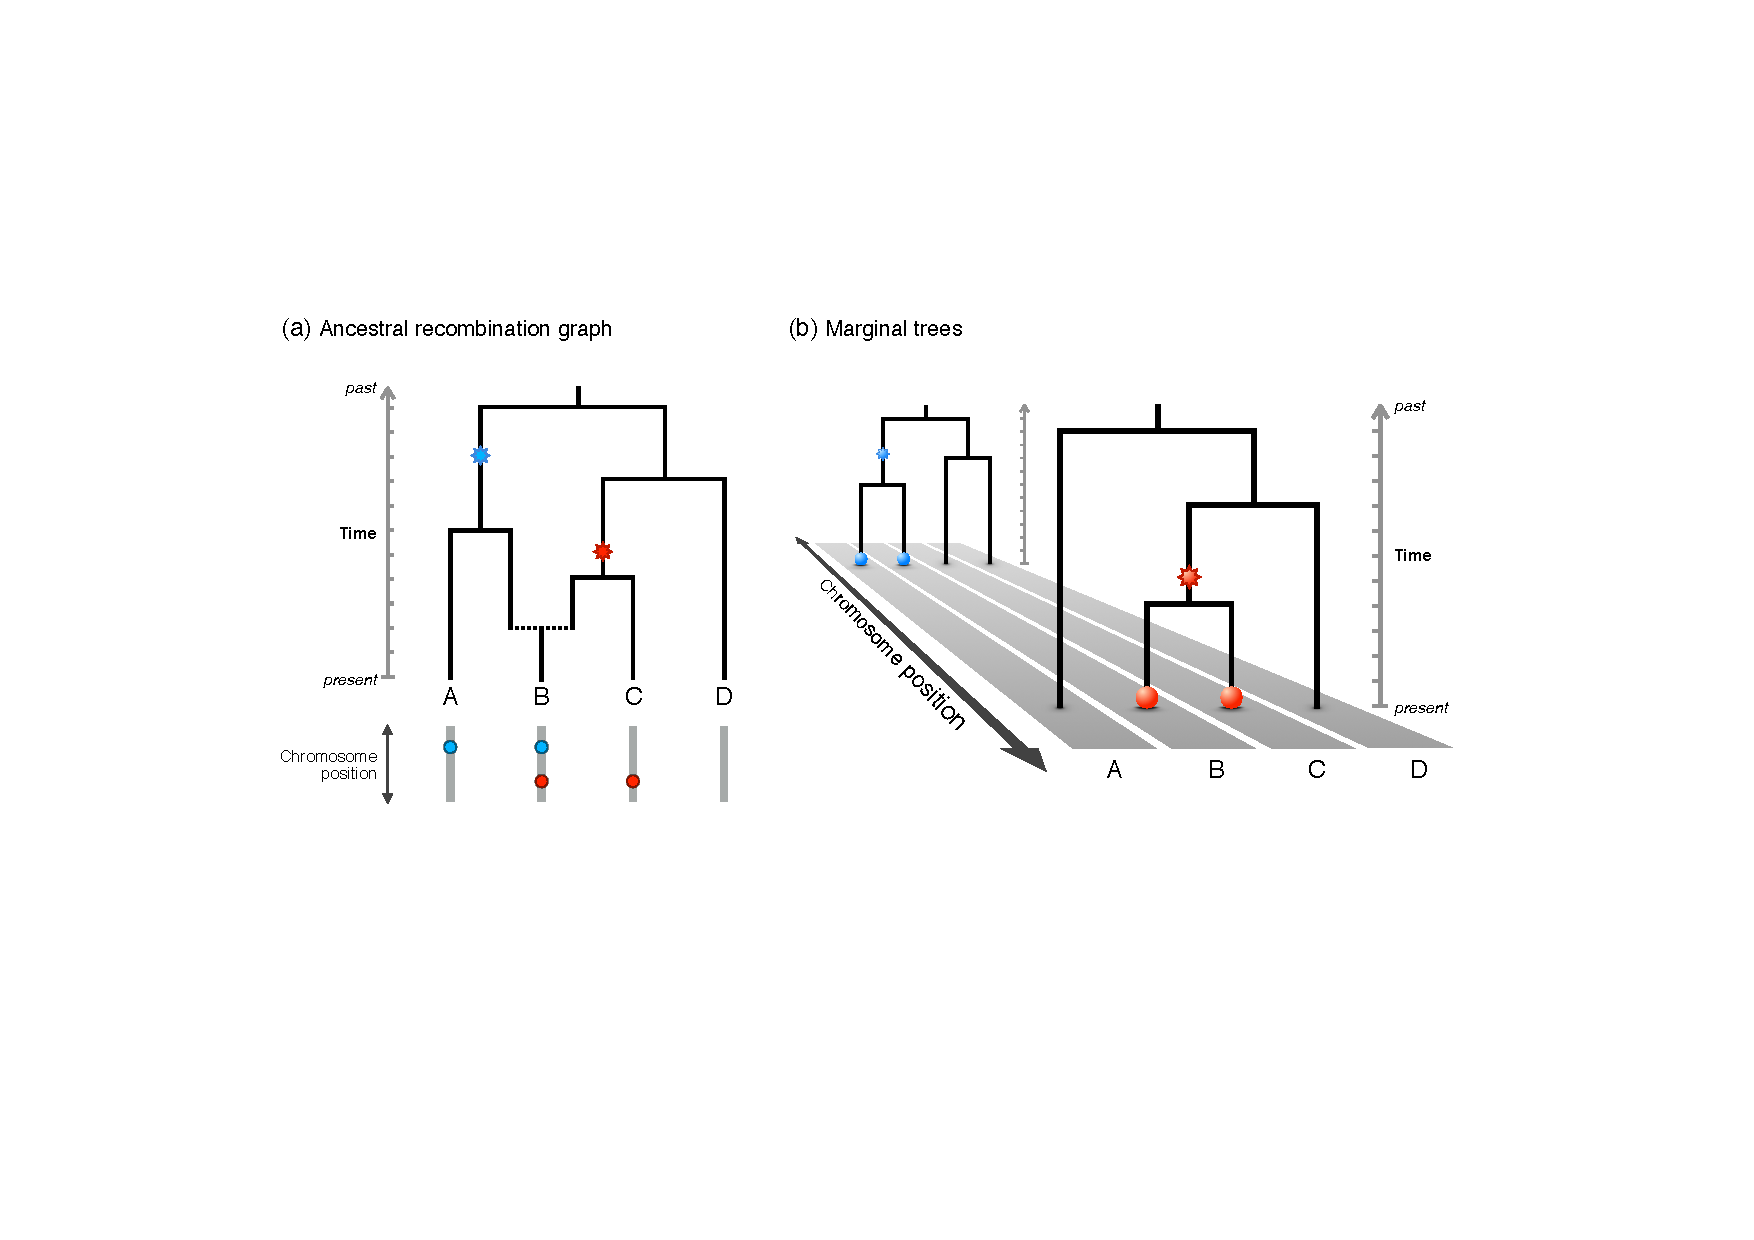
\includegraphics[width=\textwidth]{./img/ch1/info_arg}
\Caption{Illustration of the ancestral recombination graph}
{Panel~\textbf{(a)} shows the \gls{arg} for a sample of \n{4}~chromosomes, labelled by $A$, $B$, $C$, and $D$.
The \emph{dotted} horizontal line denotes the time of a recombination event between chromosomal lineages.
Mutation events are shown as \emph{stars}.
The chromosomal positions of derived alleles are indicated below the \gls{arg}.
The corresponding marginal trees are shown in Panel~\textbf{(b)}, where each lane (\emph{grey}) represents the chromosomal sequence on which the derived alleles sit (shown as \emph{marbles}).}
{fig:info_arg}
% \vspace{-5pt}
% \hrulefill%
\end{figure}

%

Given the rate of recombination per site per generation, $\rho$, the population-scaled recombination rate is given by the compound parameter
\begin{equation}\label{eq:recrate}
	\phi = 4 N \rho
\end{equation}
which is assumed to be constant in the limit ${N\rightarrow\infty}$.\footnote{Note that in the literature $r$ is often used to denote the per-generation recombination rate and $\rho$ to denote the population-scaled recombination rate.}
The factor of 4 results from time being scaled in units of ${2 N}$ generations, accounting for the fact that the population is diploid.
Note that this adjustment permeates the coalescent and implies similar changes in other equations.
For example, the scaled mutation rate given in \ctref{eq:mutrate} needs to be written as $~{\theta = 4 N \mu}~$ if considered in a diploid population.

Given a sample of $n$~chromosomes, the number of chromosomal lineages, $k$, may increase (due to recombination) or decrease (due to coalescence) back in time.
First, consider the event of no recombination and no coalescence; \ie the value of $k$ remains the same in the previous generation \citep[\eg, see][]{tavare2004}.
The probability of this event is
\begin{equation}\label{eq:coalrec_dont1}
	(1-\rho)^k~\times~\Big(1-\frac{1}{N} \Big)~\times~\Big(1-\frac{2}{N}\Big)~\times~\cdots~\times~\Big(1-\frac{k-1}{N}\Big)
\end{equation}
where ${(1 - \rho)^k}$ corresponds to the probability that none of the lineages recombine; the other terms refer to the probability of no coalescence, which was already defined in \ctref{eq:coal_n_dont}.
Now, because the rate at which \n{1} lineage branches into \n{2} lineages back in time is equal to $\rfrac{\phi}{2}$, \Cref{eq:coalrec_dont1} can be written as
\begin{equation}\label{eq:coalrec_dont2}
	1-\frac{k\phi}{2N}~-~1-{k \choose 2}\frac{1}{N}~+~\mathcal{O}\Big(\frac{1}{N^2}\Big)
	\ \text{.}
\end{equation}
For the event ${k\rightarrow k+1}$, which can only be facilitated through recombination, it follows that the probability of a recombination event in the previous generation is given by
\begin{equation}
	\frac{k\phi}{2N}~+~\mathcal{O}\Big(\frac{1}{N^2}\Big)
	\ \text{.}
\end{equation}
The term ${\mathcal{O}(N^{-2})}$ is the diffusion limit of the function and corresponds to the probability that more than \n{1} recombination event occurs at a given unit of time, which can be ignored for larger population sizes; \ie as $N$ tends to infinity.
Similarly, a coalescent event in the previous generation means that ${k \rightarrow k-1}$, for which the probability has already been described in \ctref{eq:coal_approx}.
Also, as shown in \ctref{eq:coal_n_approx}, the probability of coalescent events, in the limit ${N\rightarrow\infty}$, is exponentially distributed with rate
\begin{equation}
	{k\choose 2}~=~\frac{k(k-1)}{2}
	\ \text{.}
\end{equation}
Likewise, in the limit, recombination follows the same distribution in the coalescent at rate
\begin{equation}
	\frac{k\phi}{2}
	\ \text{.}
\end{equation}

It follows that the coalescent with recombination can be described as a continuous-time Markov chain with a \emph{birth-death} process.
Lineages are ``born'' through recombination or ``die'' due to coalescence backward in time \citep[\eg, see][]{tavare2004,wakeley2008}.
The state space is delimited by ${k=n}$ at present and ${k=1}$ at an \gls{mrca}.
The transition rates can be summarised as follows.
\begin{equation}
k ~\rightarrow~
\renewcommand{\arraystretch}{1.2}
\left\{
\begin{array}{llll}
	k-1  &  \text{at rate} & \rfrac{k(k-1)}{2} & \text{if lineages coalesce} \\
  k+1  &  \text{at rate} & \rfrac{k\phi}{2}  & \text{if lineages recombine}
\end{array}
\right.
\end{equation}
Importantly, because the rate of coalescence is quadratic in the number of lineages and the rate of recombination is at most linear, the number of lineages cannot increase indefinitely \citep{Wiuf:1997wf}.
As a result, the ancestry of all chromosomal segments are eventually traced back to a single ancestral chromosome in the ultimate \gls{mrca}.




%
\section{Advances in high-throughput genomic technologies}
\label{sec:technology}
%

In this section, I provide a brief review of the developments in high-throughput genomic technologies that have been achieved over the past 40~years.
I further highlight some of the milestone projects that have contributed substantially to our understanding of the human genome, namely the \glsentryfull{hgp}, the \glsentryfull{hapmap}, and the \glsentryfull{1kg}.
Data from \glsentryshort{hapmap} and \glsentryshort{1kg} have been used extensively in this thesis.
Note that a detailed presentation of the history and biochemistry of available technologies, as well as a comprehensive list of human sequencing projects, is beyond the scope of this chapter \citep[for review, \eg see][]{Metzker:2009ew,Naidoo:2011ip,Liu:2012hw,Mardis:2017cq}.


%
\subsection{Next-generation sequencing}
%

The first DNA-based organism to have its genome fully sequenced was the bacteriophage $\Phi\text{X174}$ (\n{5386}~basepairs), which was undertaken by \citet{Sanger:1977vp} based on the previously developed chain-termination sequencing method \citep{Sanger:1975iz}.
This technology formed the backbone of the coming era of \gls{wgs}, which has dominated the field since 1977 and was the main method employed to sequence the human genome \citep{IntHumGenSeqCon:2001hk,Venter:2001fq}.

Following the initialisation of the \glsentryfull{hgp} in 1990, and the publication of the draft sequence of the human genome in 2001, it was proclaimed in 2004 that the sequence of the human genome was ``essentially complete'' \citep{IntHumGenSeqCon:2004bm}.
However, it became clear that available technologies could not realistically be applied to generate sequence data for larger samples due to the significant requirements in labour, cost, and time.
The \glsentryfull{nhgri}, United States, therefore announced an initiative with the aim of developing novel DNA sequencing methods (awarding more than \SI{38}[\$]{million} in grants).\footnote{\textls[-25]{\url{https://www.genome.gov/12513210/2004-release-nhgri-seeks-next-generation-of-sequencing-technologies/}} \accessed{2017}{03}{15}}
Ultimately, it was hoped to decrease the cost of sequencing to \SI{1000}[\$]{} or less per genome \citep{Mardis:2006ku}.
As a result, major advances have been made in the development of commercially available sequencing and genotyping technologies, which fostered a groundbreaking synergistic relationship between research and industry, and several large-scale international projects have been initiated; see \cpref{fig:info_seqtech}.

%
%!TEX root = ../../main.tex


\begin{figure}[!htb]
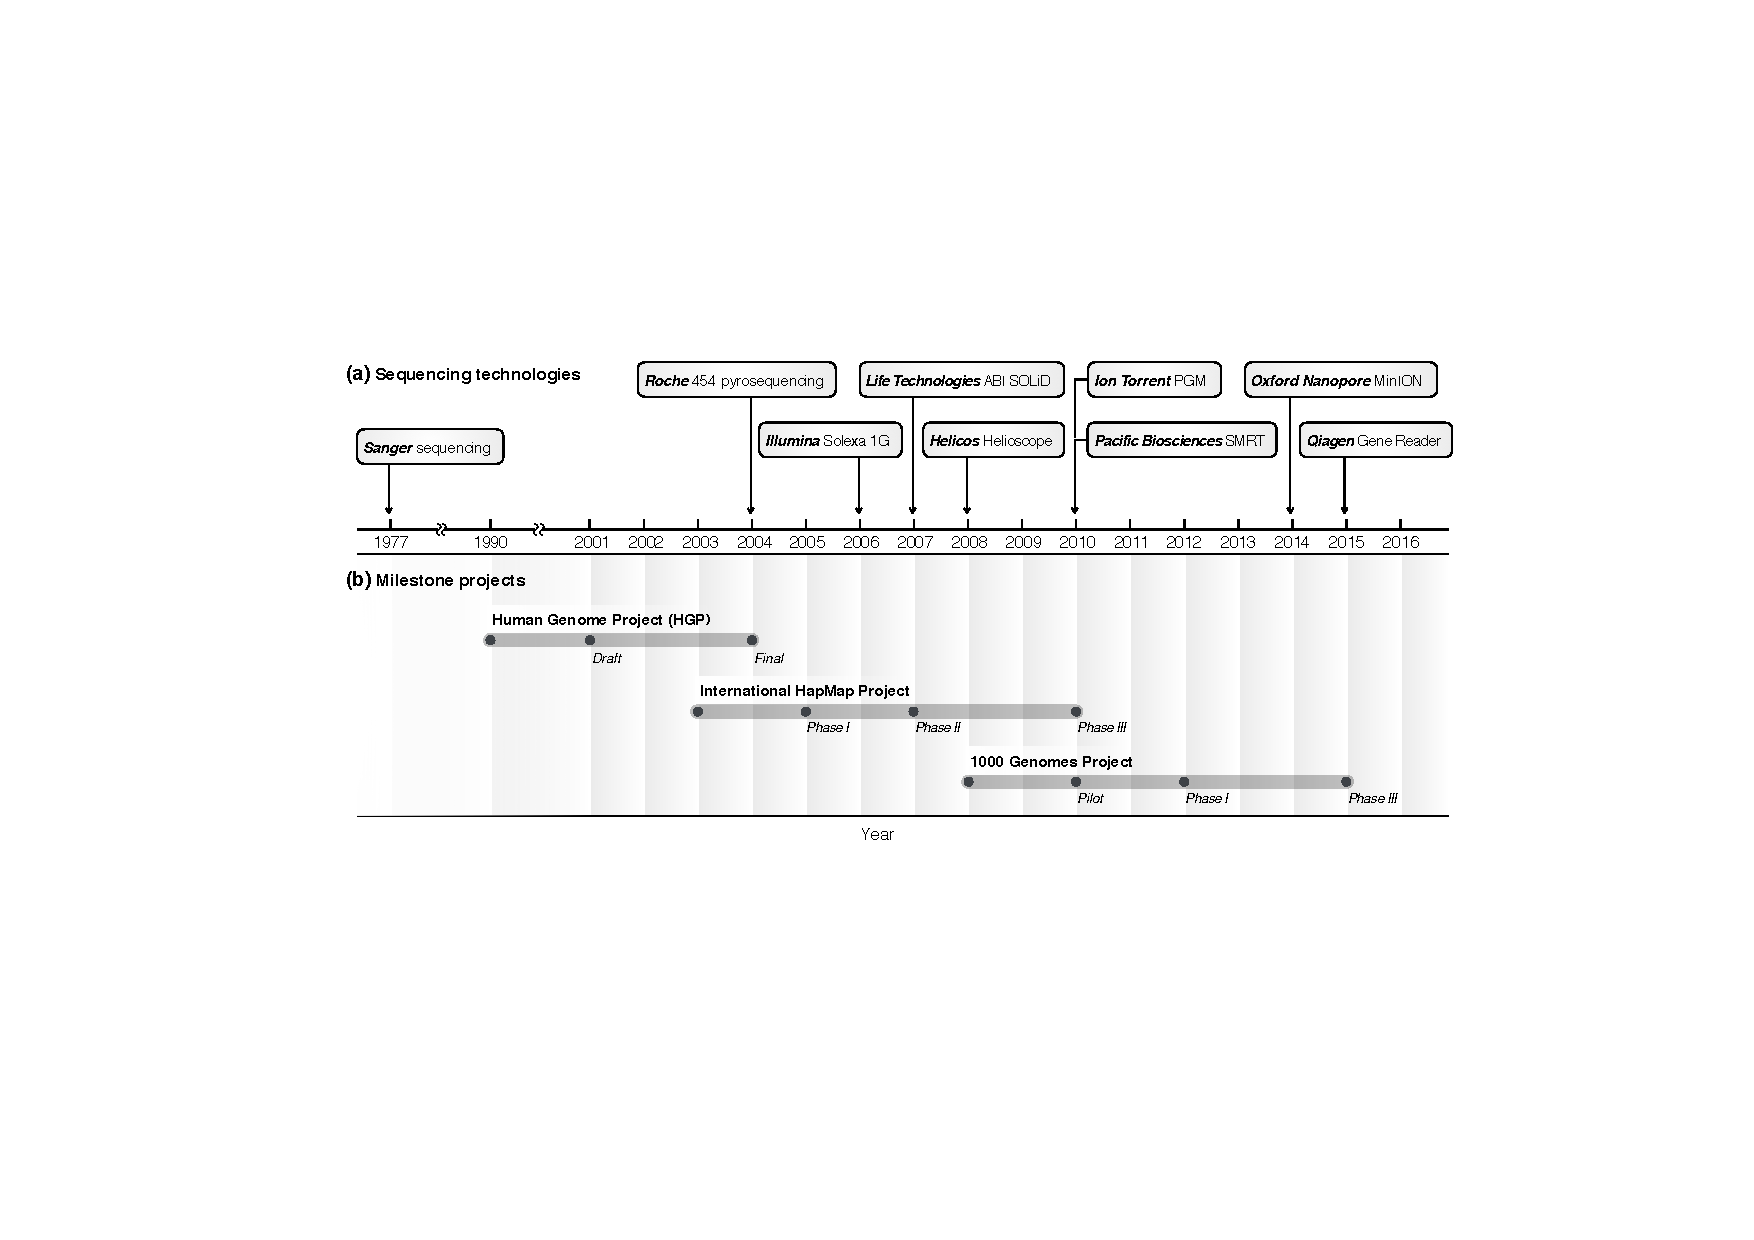
\includegraphics[width=\textwidth]{./img/ch1/info_seqtech}
\Caption{Timeline of sequencing technologies and milestone projects}
{Panel~\textbf{(a)} shows the year of commercial introduction of successfully established \gls{ngs} platforms until 2016, following the introduction of the \citet{Sanger:1977vp} sequencing method.
Panel~\textbf{(b)} illustrates the timeline of \n{3} major projects that were undertaken to sequence (or genotype) the human genome.
Figure modified from \citet[][Figure~1]{Mardis:2017cq} and \citet[][Table~1]{Naidoo:2011ip}.}
{fig:info_seqtech}
\end{figure}

%

Sanger sequencing is now regarded as the ``first-generation'' of sequencing technologies, while more recently developed techniques are commonly referred to as ``next-generation'' sequencing (\glsentryshort{ngs}), which allow higher volumes of samples to be processed in shorter time and reduced cost \citep{Metzker:2009ew}.
The first next-generation sequencer was the \emph{Roche~GS~20 System} by \textsl{Roche~454}, so called \emph{pyrosequencing}, which became commercially available in 2004.
Novel and diverse \gls{ngs} instruments rapidly became available over the past decade; notable examples include companies such as \textsl{Illumina}, \textsl{Pacific Biosciences}, and recently \textsl{Oxford Nanopore}, to name a few.
The \gls{ngs} platforms shown in \cref{fig:info_seqtech} follow \citet{Mardis:2017cq}.

%
%!TEX root = ../../main.tex


\begin{figure}[!htb]
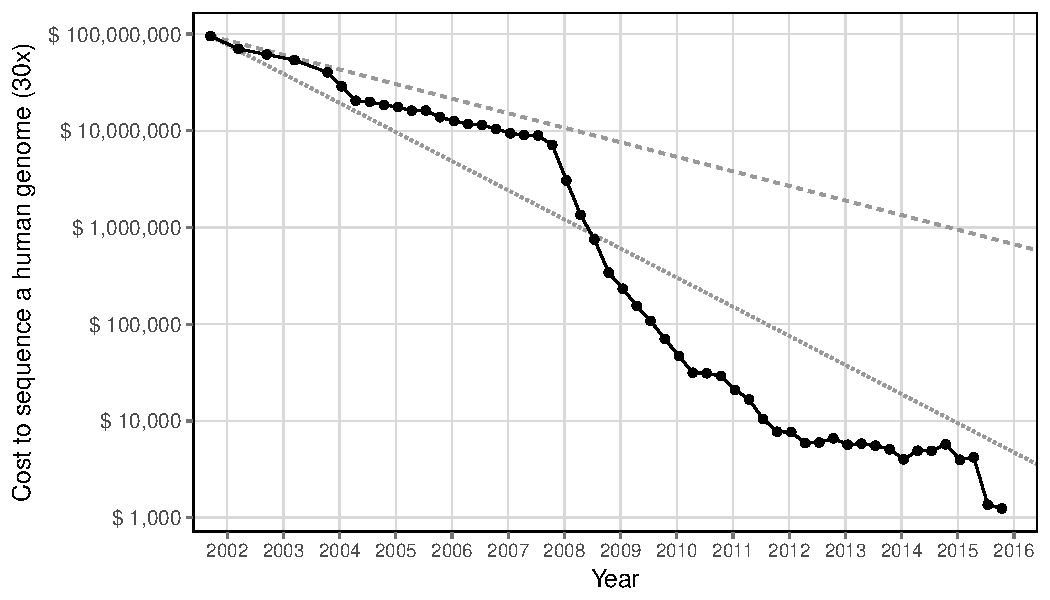
\includegraphics[width=\textwidth]{./img/ch1/cost_per_genome}
\Caption{Timeline of cost reduction in DNA sequencing}
{Technological improvements in whole-genome sequencing have led to drastic reductions in cost while simultaneously improving accuracy and speed of data generation.
The plot shows the development of price per human-sized genome sequenced at 30x depth (price given in US dollars) since the publication of the first draft sequence of the human genome in 2001.
The costs shown between 2001 and 2007 are based on the Sanger sequencing method (\emph{first-generation} methods); since 2008, costs are based on \emph{next-generation} technologies.
The hypothetically expected rate of cost reduction per genome is indicated according to Moore's law \citep{moore1965}; the price halves every \n{2} years (\emph{dashed}) or every year (\emph{dotted}).
Data provided by the \glsentryfull{nhgri}: \url{https://www.genome.gov/sequencingcostsdata/} \accessed{2017}{03}{15}.}
{fig:cost_per_genome}
\end{figure}

%

The arrival and commodification of \gls{ngs} technologies have made it feasible to sequence a whole human genome within days or weeks, rather that months or years.
There is an ongoing reduction in labour and cost, while speed and accuracy of data generation is improving.
\Delete{Interestingly, the rate at which the cost per genome is decreasing has outpaced Moore's Law, which originally predicted that the number of transistors in a dense integrated circuit would double approximately every two years.
%\citep{moore1965}.
This conjecture has been used to valuate the rate of improvement in many technological fields, where a technology is commonly regarded to progress well if it can `keep track' with this expectation.}
For example, the cost of the \gls{hgp} sequencing the first human genome has been estimated at more than \SI{3}[\$]{billion}.
The first human diploid genome (James Watson) was sequenced for less than \SI{1}[\$]{million} \citep{Wheeler:2008bb}.
Currently, the goal of the \SI{1000}[\$]{} genome is surprisingly close; see \cpref{fig:cost_per_genome}.


%
\subsection{Exploration of the human genome}
%

Our understanding of genetic information and the forces that shape variation in a population has grown substantially since the early breeding experiments on pea plants conducted by \citet{Mendel1866}, who formulated the fundamental laws of genetic inheritance, rediscovered more than \n{30}~years later \citep{correns1899,vries1900,tschermak1900}.
Yet, our patience to wait for such important insights has been decreasing exponentially.

Before the \gls{hgp} was planned, an initial human genetic linkage map had been established using \glspl{rflp} in 1980 \citep{Botstein:1980wg}.
A second-generation linkage map of the human genome had been constructed by 1993, using microsatellite markers \citep{Weissenbach:1993et}.
In 2001, \gls{ld} patterns had been documented for parts of the genome, using a combination of early sequencing methods and genotyping \citep{Daly:2001ka,Reich:2001ff}.

The release of the draft sequence of the human genome in 2001 led to numerous large-scale projects.
For example, \gls{gwa} analyses of complex diseases required the identification of genetic markers prior to interrogation; to this end, the \gls{hapmap} was initiated to validate several million \gls{snp} markers and to examine \gls{ld} patterns within different populations, eventually providing haplotype information for a representative global sample.
In addition, a central aspect of the HapMap effort was to develop methods enabling GWA analysis.

The \gls{hapmap} Project consisted of several phases of data acquisition and release.
Phase~\rom{1} involved the genotyping of 1.3~million \glspl{snp} in \n{270}~individuals from \n{4} global populations \citep{Thorisson:2005ff}.
Subsequently, Phase~\rom{2} aimed to increase the genotyping density in these same individuals to further improve the ability to map associations, supplementing the Phase~\rom{1} release with another 2.1~million \glspl{snp} \citep{Frazer:2007kha}.
In conjunction with the Human Genome Project and the SNP~Consortium \citep{McCarroll:2008dy}, approximately 11~million common \glspl{snp} had now been identified.
Finally, Phase~\rom{3} focussed on the coverage of additional populations, culminating in a total of \n{1397} samples from 11 populations (Release~3), of which \n{692} individuals had been additionally sequenced at selected regions \citep{InternationalHapMapConsortium:2010en}.

With the advantage of new \gls{ngs} technologies, the \glsentrylong{1kg} was launched in 2008, with the aim of sequencing the genomes of at least \n{1000} individuals across different populations, in order to provide a comprehensive resource of observed human genetic variation that could be leveraged by \gls{gwa} studies and research in population genetics.
The pilot phase described approximately 15~million \glspl{snp}, most of which had not been identified previously \citep{Durbin:2010gj}.
Several pilot projects were undertaken, including low-coverage \gls{wgs} of \n{179} individuals from \n{4} populations, high-depth sequencing of \n{2} trios (parents and child), and targeted exome-sequencing of \n{697} individuals from \n{7} different populations.

The variants discovered in the pilot stage were common ($>5\%$ minor allele frequency); that is, low-frequency variants were underrepresented.
It had been recognised that rare and low-frequency variants are candidates for functional mutations under weak purifying selection and therefore could further our understanding of complex disease \citep{Marth:2011bz,Tennessen:2012ck}.
To capture variants that occur at lower frequencies per population sample, it was necessary to sequence hundreds or thousands of genomes \citep{Kaiser:2008wd}.

%
%!TEX root = ../../main.tex


\begin{figure}[!htb]
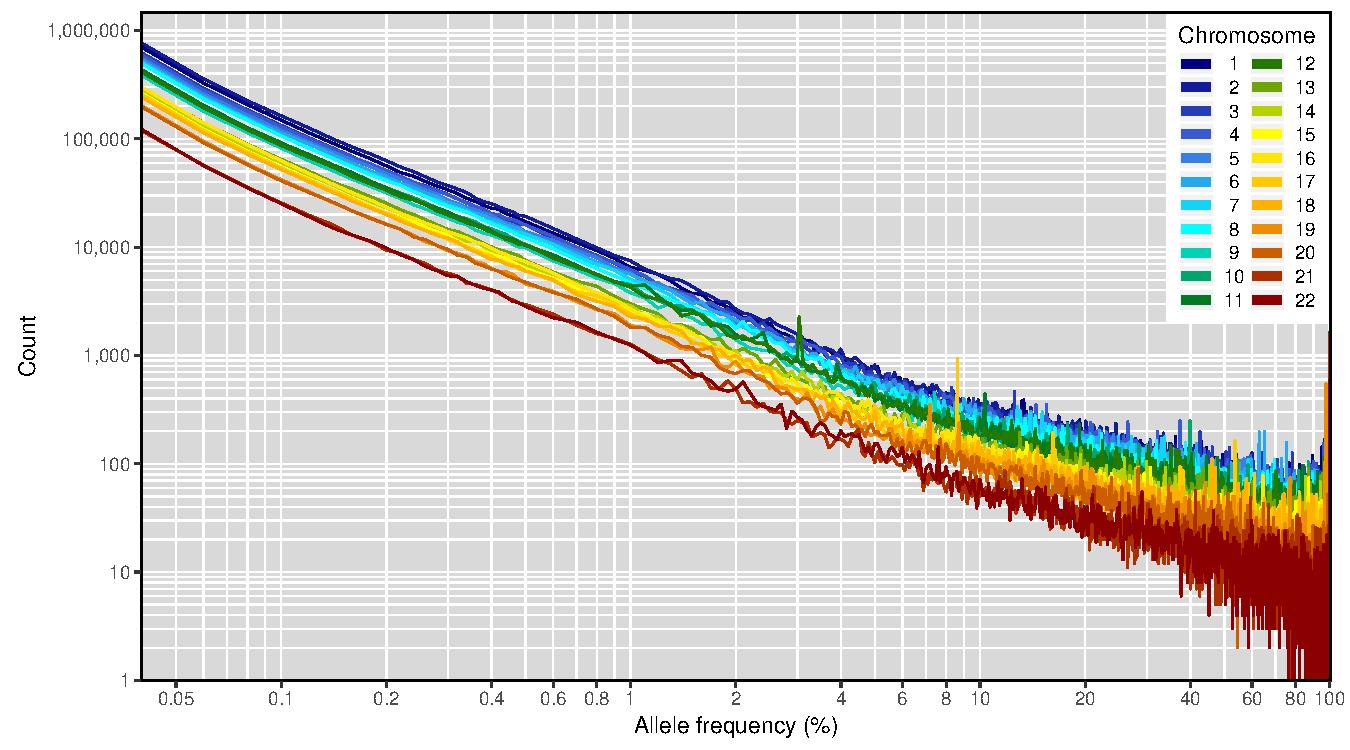
\includegraphics[width=\textwidth]{./img/ch1/allelefreq_1kg}
\Caption{Allele frequency spectrum in the 1000 Genomes Project}
{The allele frequency distribution is shown per chromosome (1--22) for all variants contained in the final release dataset of \gls{1kg} Phase~\rom{3}.
Singletons (private mutations observed only once in the sample) were excluded.
Note that data are shown on log-log scale.}
{fig:allelefreq_1kg}
\end{figure}

%

This led to Phase~\rom{1} of the \glsentrylong{1kg}, carried out on \n{1029} individuals from \n{14} populations, and comprising a combination of low-coverage \gls{wgs}, targeted exome sequencing, and genotyping by microarray.
This resulted in the profiling of 38~million \glspl{snp} in total, with the majority being rare \citep{GenomesProjectConsortium:2012co}.
Phase~\rom{2} of the project focussed on methods development, while increasing the sample size to \n{1700} indivudals; these methods were applied to a total of \n{2504} samples from \n{26} populations in Phase~\rom{3}, leading to a final release dataset of 84.7~million \glspl{snp} and the completion of the project \citep{Auton:2015gk}.
\Cpref{fig:allelefreq_1kg} illustrates the allele frequency spectrum of all variants identified through the \glsentrylong{1kg} (final release, Phase~\rom{3}); shown per chromosome after removal of private mutations (singletons).



%
\section{Genome-wide association studies}
\label{sec:gwas_intro}
%

The \glsentrylong{hapmap} was instrumental to the design of \gls{gwa} studies by validating millions of \glspl{snp} in the human genome and revealing the structure of genetic variation through patterns of \gls{ld} in different populations.
Due to the non-independence of markers, association analyses may only interrogate a modest subset of variants to detect common risk alleles.
It was shown that the efficiency of \gls{gwa} studies could be maximised by scanning only a fraction (${\approx 1\%}$) of the 11~million \glspl{snp} that were known at that time \citep{deBakker:2005cy,Peer:2006bk}.
The availability of \gls{hapmap} data was used to guide the development of genotyping arrays, to tag \glspl{snp} markers that are informative to capture most of the variation between individuals.

%
%!TEX root = ../../main.tex


\begin{figure}[!htb]
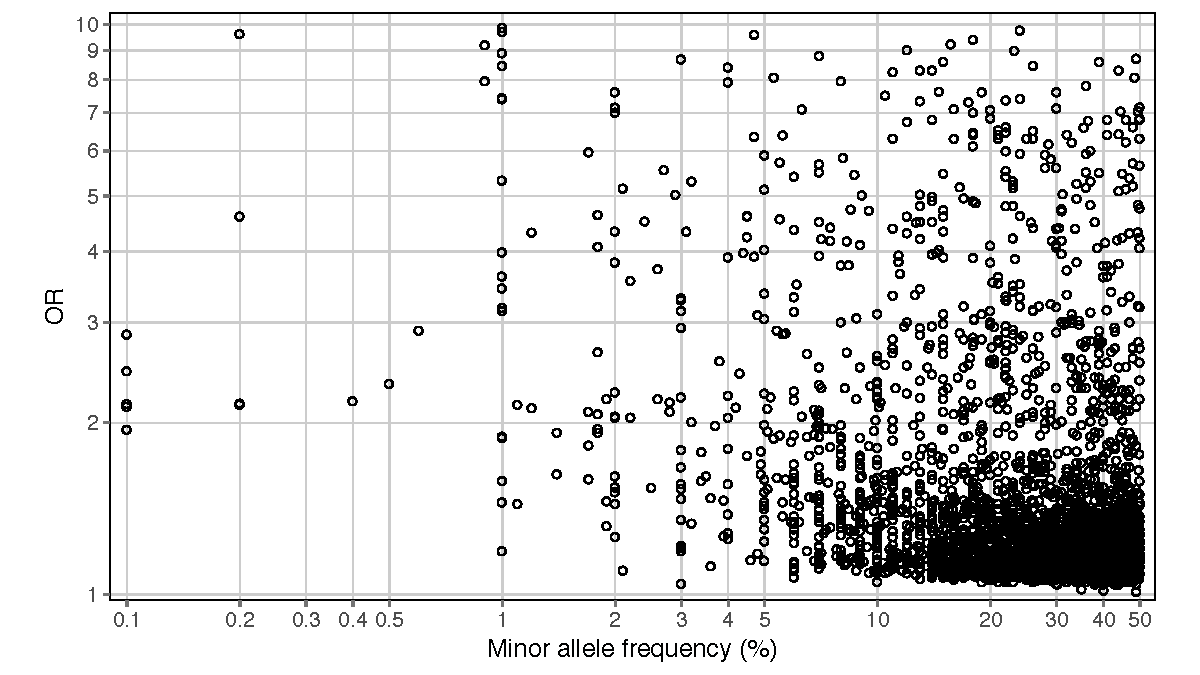
\includegraphics[width=\textwidth]{./img/ch1/gwascat}
\Caption{Significant risk-associated variants listed in the NHGRI-EBI Catalogue}
{Results are shown for \n{3186}~unique variants which were reported as being significant at ${\pvalue\leq\num{5e-8}}$ and for which \gls{or} values were available in the database.
Note that different studies may report different \gls{maf} and \gls{or}.
Duplicate entries (variants reported in more than \n{1} study) were removed, after calculating the median value of \gls{maf} and \gls{or} across duplicates; frequencies were then rounded to \n{3} decimal places.
Data were taken from \url{http://www.ebi.ac.uk/gwas/} \accessed{2017}{01}{20}.}
{fig:gwascat}
\end{figure}

%

The first proper \gls{gwa} study was undertaken by \citet{Klein:2005dn}, who successfully identified a common variant of large effect size to be significantly associated with age-related macular degeneration.
The number of subsequent \gls{gwa} studies rapidly increased; by 2007, more than \n{100} studies had been published, which was considered as the ``breakthrough of the year'' by \textsl{Science} \citep{Pennisi:2007cs}.
Currently, the GWAS Catalogue maintained by the \gls{nhgri} and the \gls{ebi} lists \n{2324} publications and reports more than \n{30000} unique \gls{snp} associations of which more than \n{8000} are significant at ${\pvalue\leq\num{5e-8}}$ for approximately \n{1000} traits \citep{burdett2016nhgri}.\footnote{NHGRI-EBI GWAS Catalogue: \url{http://www.ebi.ac.uk/gwas/} \accessed{2017}{01}{20}}
The bulk of these results is summarised in \cpref{fig:gwascat}, in which I show the relation between risk effect size and allele frequency for identified risk-associated variants at ${\pvalue\leq\num{5e-8}}$.

%
%!TEX root = ../../main.tex


\begin{figure}[!htb]
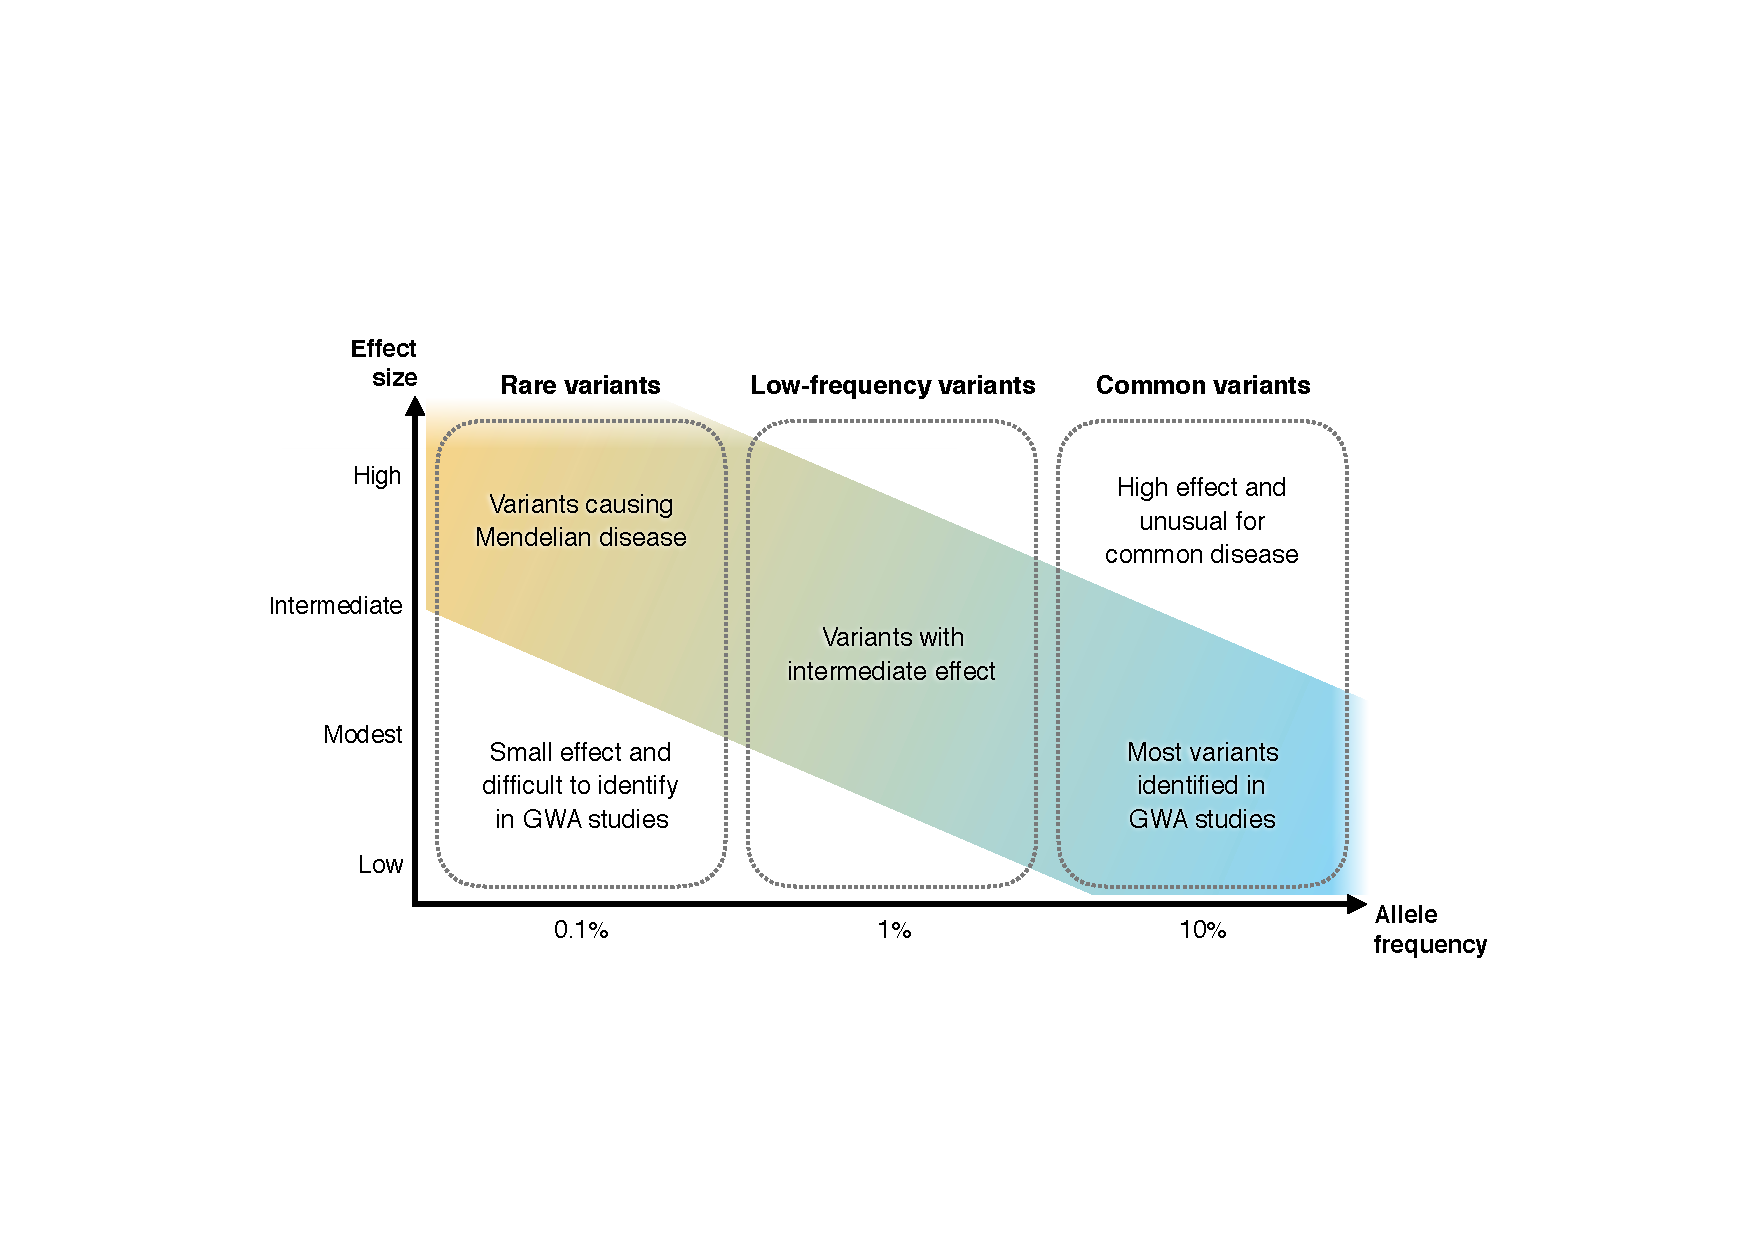
\includegraphics[width=\textwidth]{./img/ch1/gwa_spectrum}
\Caption{Risk-related variants by allele frequency and effect size}
{Rare, low-frequency, and common variants are distinguished by (minor) allele frequency.
Note that frequency values are only indicated as approximate guides.
Figure adapted from \citet[][Box~7]{McCarthy:2008il} and \citet[][Figure~1]{Manolio:2009jp}.}
{fig:gwa_spectrum}
\end{figure}

%

In contrast to traditional linkage approaches, which have high power to locate low-frequency variants of large effect size (\eg Mendelian diseases), \glsentrylong{gwa} was designed and has proven to be powerful for interrogating common variants with modest effects.
This disparity is illustrated in \cpref{fig:gwa_spectrum}, which outlines a seemingly categorical distinction between rare, low-frequency, and common variants based on expected penetrance and the ability to detect effects resulting from such genetic factors.
The limitations of both approaches lie at the extremes (outside the band indicated in \cref{fig:gwa_spectrum}).

Notably, rare variants with modest or low penetrance are difficult to detect by either linkage or \gls{gwa} analysis.
Since it became apparent that the human genome harbours an abundance of rare and low-frequency variants, it has been suggested that there might be unexpectedly large amounts of deleterious rare variants with low to modest effects \citep{Coventry:2010cqa,Keinan:2012kl,Tennessen:2012ck}.
Using \gls{gwa} methods, the interrogation of alleles observed at very low (rare) frequencies may represent a conceptual limitation, however, it is hoped that the detection of low-frequency variants with intermediate effect can be improved.


%
\section{Identity by descent}
\label{sec:ibd_definition}
%

Relatedness among individuals is a natural property of genetic inheritance.
Although this observation may seem trivial as we all inherit our DNA from somebody,\footnote{Until CRISPR/Cas9 genome editing has been established \citep[\eg see][]{Cai:2016km}; in reference to the term \emph{\glsentrylong{ibd}}~(IBD) I propose the term \emph{identity by modification}, or IBM. {\color{oxgray}[\textit{Castigat ridendo mores}]}} knowledge about the genetic relationship between individuals is crucial to many applications in genetic research.
The validation of individual relationships is of particular interest in family-based methods such as linkage analysis \citep{Purcell:2007dg,Albrechtsen:2009cb}, or to exclude pedigree errors that would influence statistical power in linkage studies \citep{Boehnke:1997ku}, but also in population-based (case-control) association studies of purportedly unrelated individuals, where unreported relatedness may lead to spurious results due to population stratification, \ie systematic differences in the ancestry of individuals \citep{Freedman:2004dk,Voight:2005cr}.

The relationship between individuals is indicated by the alleles they have in common, where \n{2} alleles are said to be \emph{identical by descent} if they have been co-inherited from a common ancestor \citep{Thompson:1974fi,Thompson:1975uu}.
The concept of \glsentryfull{ibd} was introduced by \citet{cotterman1940calculus} and extended by \citet{malecot1948mathematics} who provided probability formulations of IBD in related individuals; the term ``identity by descent'' was coined by \citet{crow1954}.
Notably, \citet{malecot1948mathematics} defined IBD as the probability that no mutation occurred since the common ancestor; see also \citet{Slatkin:2008by}.
In contrast, \gls{ibs} refers to alleles that are observed to be the ``same'', but which may not be shared by descent.

%
\subsection{Single-locus concept}
%

Traditional measures of relatedness define IBD as the gametic relationship at a single locus, for which in particular the inbreeding coefficient and the kinship coefficient introduced by \citet{Wright:1921tk,Wright:1922cr} have been relevant.
For example, the probability that \n{2} homologous alleles are identical by descent in the same diploid individual is given by the inbreeding coefficient.
However, such traditional approaches often assume that the relationship status of the individuals is known or can be derived from possible pedigree relationships, where ancestors are defined with respect to the founders of a pedigree.
It has been argued that ancestry defined in reference to a founder sample is ``something arbitrary'' \citep[][p~141]{maynardsmith1989}; see \citet{Rousset:2002bz}.
Moreover, this definition of IBD (in particular the distinction between IBD and IBS) seems to be in conflict with coalescent theory, which postulates that every allele is technically identical by descent in the individuals which carry them, because all shared mutations in the genome can be traced back to a common ancestor at different times in the past \citep{Powell:2010di}.

%
\subsection{Genealogical concept}
\label{sec:genealogical_ibd}
%

Given the recent advances in genomic technologies, single-locus concepts of IBD have become less common and are supplanted by genealogically defined concepts of \emph{haplotype sharing by decent} in large samples of unrelated individuals \citep{Thompson:2013cj,Wakeley2016book}.
For example, the inference of IBD sharing has been useful to provide information about historical migration events and to reconstruct the demographic history of a population \citep{Palamara:2012cya,Palamara:2013eg,Harris:2013id}.

%
%!TEX root = ../../main.tex


\begin{figure}[p]
{\small\texthv{\textbf{(a)}}} \\
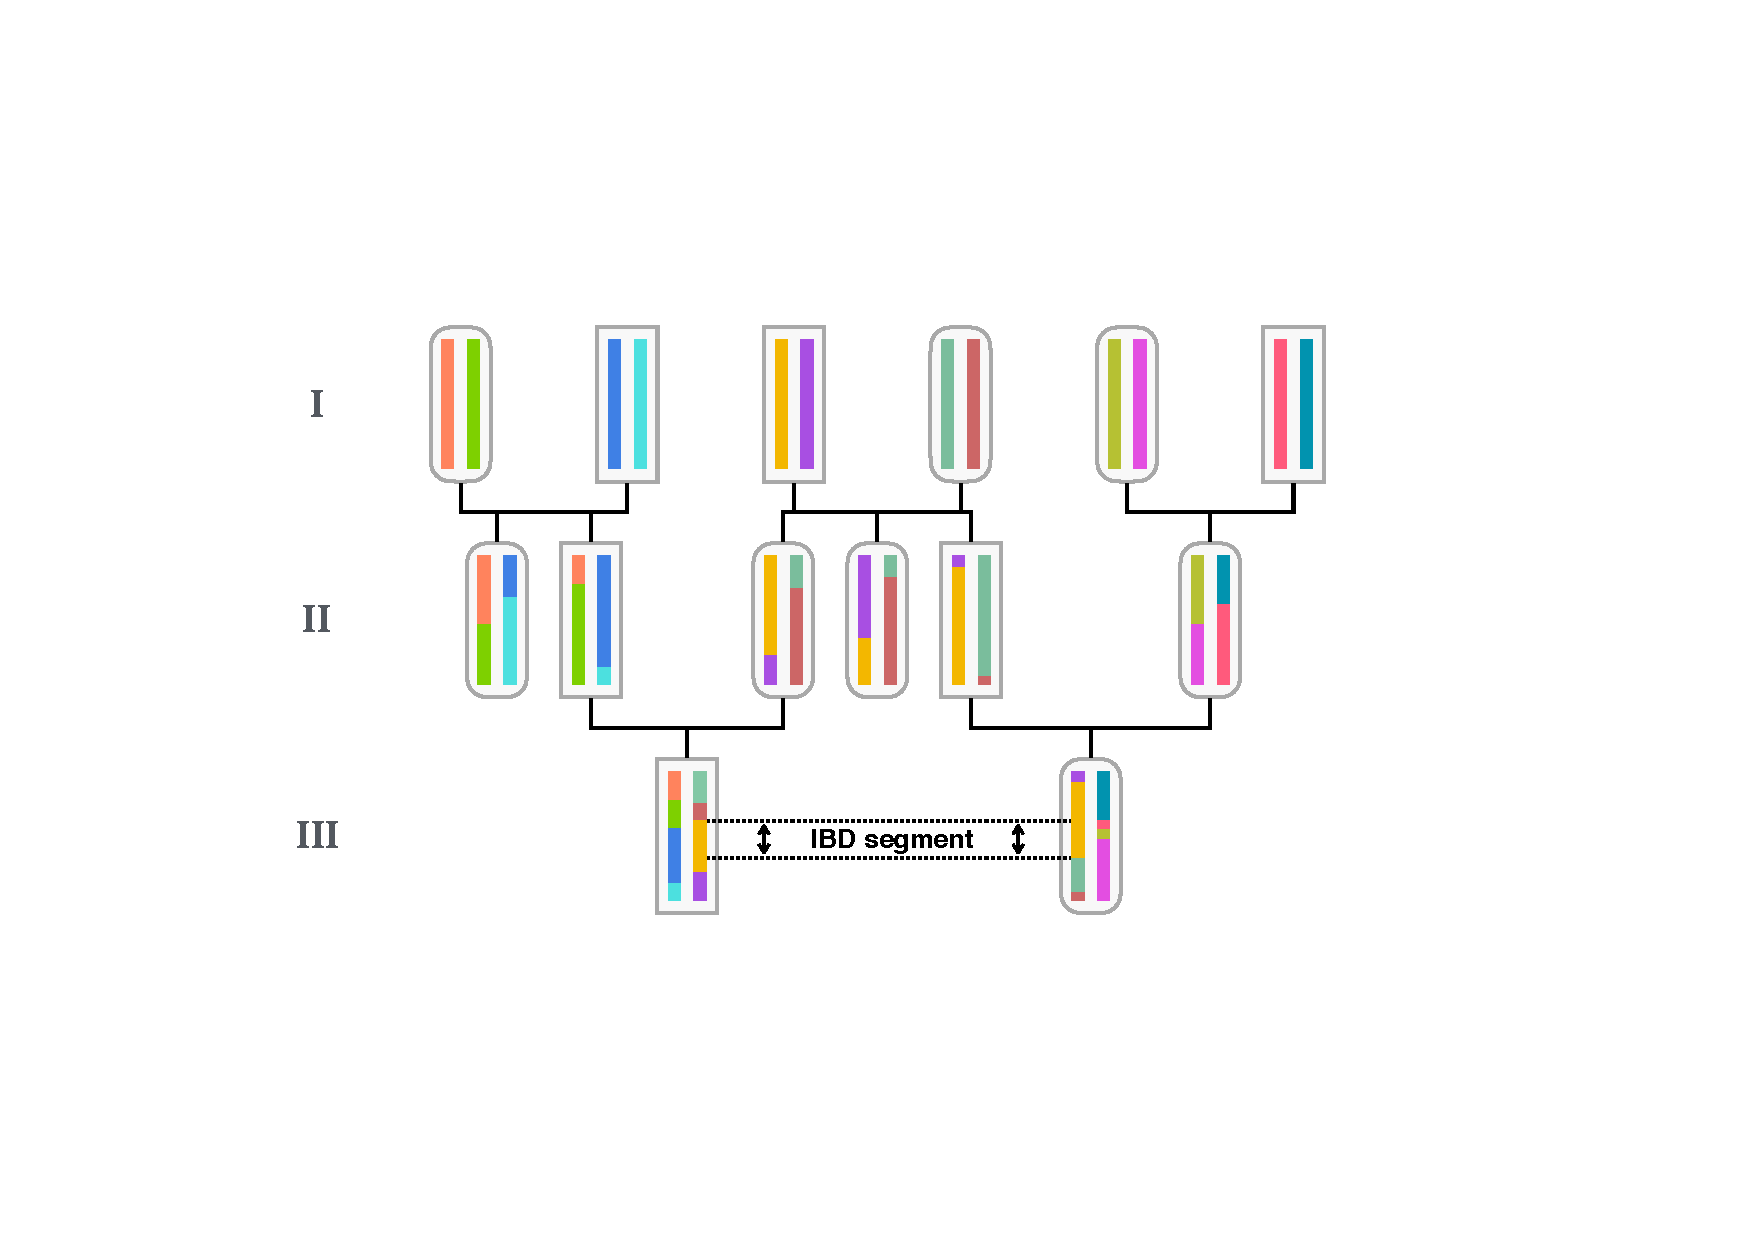
\includegraphics[width=\textwidth]{./img/ch1/info_ibd}
{\small\texthv{\textbf{(b)}}} \\
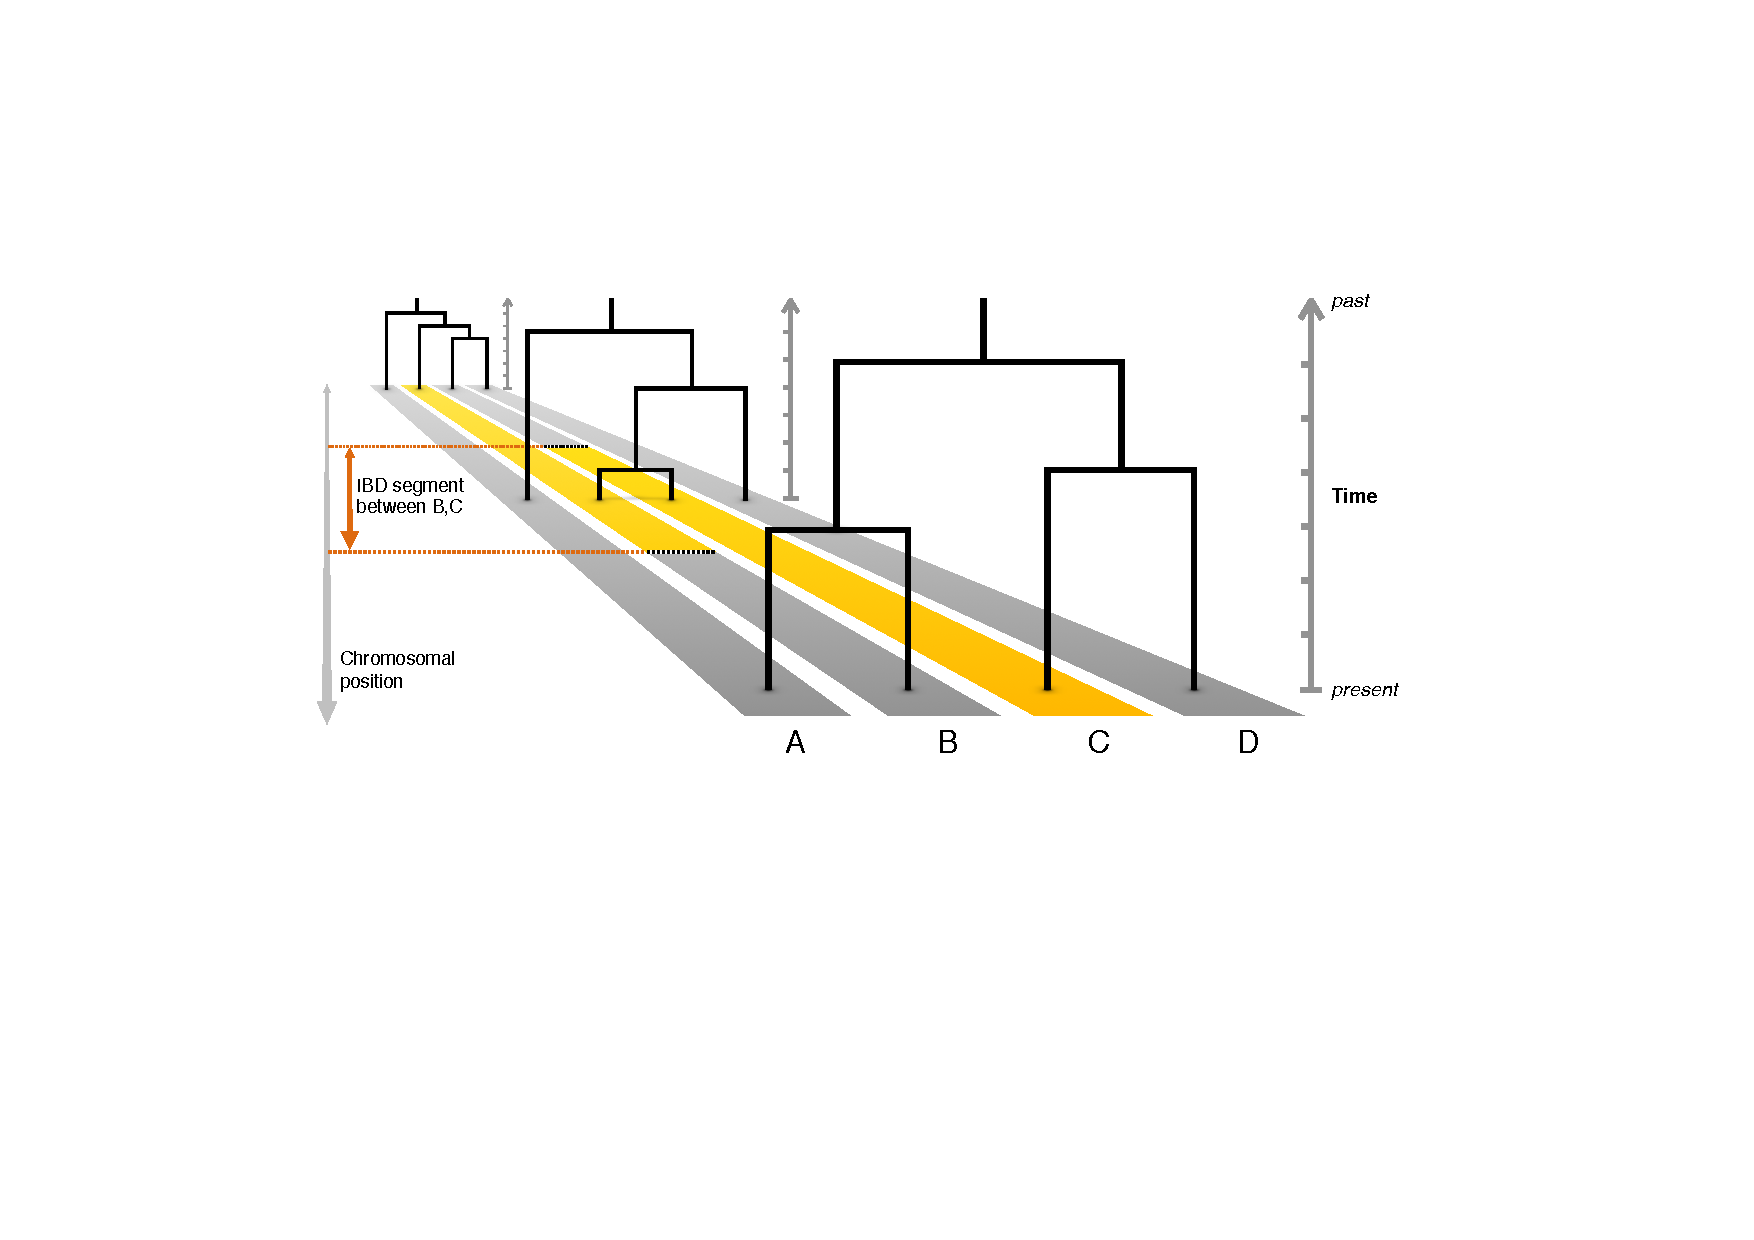
\includegraphics[width=\textwidth]{./img/ch1/info_ibd_segment}
\Caption{Illustration of haplotype sharing by descent}
{Panel~\textbf{(a)} shows a \n{3}-generation pedigree; generation~\rom{1} consists of the founders of the pedigree.
The \n{2} individuals shown in generation~\rom{3} are first-degree cousins.
Male and female individuals are distinguished by square and round shapes, respectively.
Each individual carries a diploid genome, shown as \n{2} large homologous chromosomes.
The colour of each chromosome indicates the ``identity'' of the shared ancestral haplotype, which is shuffled with the other haplotype present in the same individual due to meiotic recombination in each generation, such that the offspring receives a unique arrangement of haplotype segments per chromosome from each parent.
The ``shared'' haplotype refers the the overlapping region of haplotypes that are identical by descent; \ie the IBD segment shared by the \n{2} individuals in generation~\rom{3}, indicated by the \emph{orange} ancestral haplotype.
For simplicity, all founders are shown with the same colour.
Panel~\textbf{(b)} illustrates the different genealogies along the length of the sequence of \n{4} chromosomes (A, B, C, and D), indicated by \n{3} marginal trees.
The IBD segment co-inherited by chromosomes B and C is found at the overlapping region of the shared ancestral haplotype of the \gls{mrca} (\emph{orange}).
Note that the \n{4} chromosomes given in Panel~(b) show a simpler arrangement of haplotypes than shown in Panel~(a).}
{fig:info_ibd}
\end{figure}

%

If an allele at a given locus has been co-inherited (recently) by \n{2} or more individuals, it is likely that alleles at the surrounding loci on the same chromosome were also derived from the same ancestral lineage in those individuals.
The definition of IBD is therefore extended to refer to homologous chromosomal \emph{segments} that are identical by descent if they have been co-inherited without intervening recombination from a common ancestor \citep{Hayes:2003gj,Powell:2010di}, such that the genealogical relationship between \n{2} haplotypes is the same along the shared region.
Consequently, meiotic recombination is seen as the driving force that shapes the patterns of relatedness among individuals.
The length of a shared IBD segment is delimited by recombination events that occurred independently in each lineage; IBD therefore results from the unique pairwise relationship between \n{2} gametes.
To illustrate the genealogical concept of IBD, consider the example shown in \cpref{fig:info_ibd}.

Note that recombination events may not always result in the termination of an IBD segment.
This is because a coalescent event may join the \n{2} lineages broken up by recombination back together (back in time), forming a `closed loop' in the \gls{arg} \citep[see][Theorem~2.4]{griffiths1997ancestral}.
Further, haplotype segments that are identical by descent may not actually be ``identical'', because the alleles observed along the shared sequence may differ.
This is because mutations accumulate along each lineage independently, such that IBD segments separated by many meioses carry an increasing number of pairwise mutational differences.
Likewise, it is expected that the length of the shared segment is decreasing over time due to recombination.
As such, the ``signal'' of IBD might be lost for relatively old relationships, which can be described as the genetic ``event horizon''.
In practice, the detection of IBD segments is therefore often limited to recently inherited shared haplotypes (\eg $<100$ generations); see \citet{Browning:2008es}.



%
\section{Allele age estimation}
\label{sec:alleleage}
%

There has been growing interest in being able to estimate the age of alleles that segregate in contemporary human populations; that is, the time since an allele was introduced into a population through a mutation event.
The age of an allele, in conjunction with patterns of allele sharing, would allow us to better understand human evolutionary history and past demographic events and processes.
It has been suggested that by knowing the age of alleles, geneticists will be able to build a ``time machine'' to explore our past \citep{Slatkin:2000us}.

A number of mechanisms can affect the frequency at which an allele that emerged at some unknown point in the past is observed in a population.
For example, an allele might be under purifying selection and hence on its way to becoming extinct.
Conversely, it might endow a selective advantage and is therefore increasing in frequency.
If the allele is neutral it could be subject to random genetic drift or simply be present due to a founder effect.
Finally, the heterozygous state might have a selective advantage, meaning that the allele is held at a steady frequency in the population despite being ``old'' \citep{Colombo:2007ba}.


%
\subsection{Theoretical results}
%

The field of population genetics has been fascinated with the possibility of estimating the time of mutation events.
Early and often purely theoretical approaches had been conceived prior to the discovery of the coalescent.
For example, \citet{Kimura:1973ug} found that the frequency of \Correct{an} allele can be used as an estimator for its age, which they derived in a diffusion process.
The expected age of a neutral allele in a constant population is given by
\begin{equation}\label{eq:intro_kimura_ohta}
	\mathbb{E}\left[t_m\right]~=~\frac{-2x}{1-x}~\log(x)
\end{equation}
where $x$ denotes the frequency of an allele observed in a sample; the age, here denoted by~$t_m$, is scaled in units of~$2N$.
Notably, this and other contributions to the field by Kimura were deserving of a dedicated review \citep{Watterson:1996wr}.

Related results were provided by \citet{Maruyama:1974ba} and \citet{Li:1975vj}, who considered allele age as a random variable for which the probability of reaching fixation or extinction is regarded in presence of selection (\ie assuming that the allele is beneficial or deleterious, respectively).
Using diffusion methods, they have shown that (purifying) selection reduces the average age of an allele, whereas mutations that increase fitness also increase the average age.
\Citet{watterson1976} further developed the theory to provide the probability distribution of allele age conditional on its frequency; see review by \citet{Slatkin:2000bi} and \citet{Slatkin:2000us}.

An alternate approach was proposed by \citet{Thompson:1976uf}, who considered the age of an allele as a fixed parameter to derive the likelihood function for the age using a discrete branching process model, given the number of allele copies found in a sample.
Notably, \citet{Thompson:1976uf} has shown that it is unrealistic to arrive at an exact point estimate for the age of a given variant in a sample, due to the stochastic nature of genetic evolution in natural populations.
However, it is possible to derive a confidence interval to delimit the period during which a mutation event is likely to have occurred.

Later, \citet{Griffiths:2013ec} extended these earlier results in context of the coalescent.
For example, the following formulation describes the expected age of an allele under a constant population size and the assumption of the infinite sites model \citep{Kimura:1969tn,Watterson:1975ur};
\begin{equation}\label{eq:intro_griffiths_tavare}
	\mathbb{E}\left[t_m\right]~=~2~{{n-1}\choose{b}}^{-1}~\sum_{j=2}^{n}~{{n-j}\choose{b-1}}~\frac{n-j+1}{n(j-1)}
\end{equation}
which is equivalent to \cref{eq:intro_kimura_ohta} and provides conform estimates based on allele frequency alone.
Nonetheless, a general conclusion reached by the field was that the distribution of allele age based on its frequency alone is too broad to provide reliable age estimates, which meant that there was only little practical utility \citep[see][]{Slatkin:2000bi}.

However, due to the growing interest in exploring the genetic and genealogical basis of human disease, several other methods have been developed, most of which based on \emph{intra-allelic variability}, which is defined as the extent of variability observed at closely linked markers \citep{Slatkin:2000us,Slatkin:2001wr}.
Note that this idea can be seen as a progenitor to the genealogical IBD concept presented in the previous section (\pref{sec:genealogical_ibd}); that is, before recombination had been first mentioned in the definition of IBD \citep{Hayes:2003gj}.\footnote{Note that the connection between identity by descent, linkage, and recombination had been anticipated long before \citep[\eg see][]{Donnelly:1983fi}.}
These methods have been applied to numerous cases, some of which are summarised in the following section.


%
\subsection{Application in human disease research}
%

I provide \n{3} examples of studies in which the age of an allele has been estimated.
The first \n{2} studies below represent early examples that have been conducted in context of a specific disease on limited data; \ie prior to the high-throughput sequencing era.
The third and more recent study was conducted ``blindly'', in a hypothesis-generating approach on more than a million protein-coding variants using exome-sequencing data, without targeting specific loci of known disease association.

\Citet{Serre:1990uy} analysed the ${\Delta{F508}}$ mutation of the \textsl{CFTR} gene, which had been identified as causing cystic fibrosis, and is higher in frequency in European populations compared to other populations.
They used \glsentryfull{rflp} data from \n{240} French families, estimating the age from the variation observed at \n{2} linked loci.
As a result, they estimated this mutation to have occurred \n{3000} to \n{6000} years ago, which was consistent with an estimate of approximately \n{3000}~years found by \citet{Slatkin:2000us}, who replicated the study on intronic microsatellite data provided by \citet{Morral:1994vx}.

\Citet{Risch:1995ir} examined \n{6} closely linked microsatellite markers in data from \n{59} Ashkenazi Jewish families with idiopathic torsion dystonia (ITD), a rare disorder involving involuntary and sustained muscle contractions.
They showed that cases with early-onset ITD (Oppenheim's dystonia) are due to a single founder-mutation, which they estimated to have emerged around \n{350} years ago, during a period when the population was geographically restricted to historic Jewish settlements in northeastern Europe.

More recently, \citet{Fu:2012hg} used exome data from \n{6515} individuals and estimated the age of more than 1~million protein-coding \glspl{snp}, using a simulation-based approach under several established demographic models.
In addition, they predicted whether variants were deleterious using a range of different methods, Interestingly, they found that the probability that a variant was predicted to be deleterious was strongly related to estimated allele age.
\Citet{Fu:2012hg} found that some of the genes surveyed, among those which had been associated with human diseases, showed a significant excess of putative deleterious variants which were estimated to have a relatively recent origin through mutation.
For example, several of those genes had been implicated in coronary artery atherosclerosis (\textsl{CPE}), hereditary spastic paraplegia (\textsl{KIAA0196}), premature ovarian failure (\textsl{LAMC1}), and Alzheimer's disease (\textsl{LRP1}).
In fact, the majority of identified deleterious variants within gene-coding regions were rare in frequency, enriched for mutations of large effect size, and indicated to have emerged relatively recently, within in the last \n{5000} to \n{10000} years.

In general, it has been argued that the observed excess of deleterious rare variants in the human genome is due to a recent, explosive population growth, following a bottleneck population size after the expansion out of Africa, \n{50000} to \n{100000} years ago, and the advent of agriculture, approximately \n{10000} years ago \citep{Coventry:2010cqa,Keinan:2012kl,Tennessen:2012ck}.
For example, the effects of (weak) purifying selection can be considered as being too slow to purge young alleles with disadvantageous phenotypic consequences from the population, such that there might be an unrecognised large abundance of rare variants in the human genome which could influence disease risk in yet unaccounted ways.
An argument to the contrary, however, suggests that recent demographic changes such as population growth may have had negligible impact on the mutational load carried by an individual on average \citep{Simons:2014fj}.
As such, the amount of ascertained rare variants may not necessarily contribute to complex disease risk unless they exert strongly deleterious effects on fitness.
Thus, it remains to be seen whether rare variants play an important or an inconsequential role with regard to complex disease susceptibility; to that end, knowledge about their age may lead to a better understanding of disease aetiology.
Regardless, the estimation of allele age still remains a matter of curiosity.

% !TEX root = ../main.tex

\glsresetall


\topquote[8cm]{
We chose it because we deal with huge amounts of data. \\
Besides, it sounds really cool.
}{Larry Page, co-founder of Google Inc.}


%\chapter{A method to combine genotype data imputed from multiple references}
%\chapter{A method to combine imputed genotypes from multiple reference panels}
{
\singlespacing
\chapter{Meta-imputation of reference data to increase accuracy and power in association analysis}
\label{ch:metaimpute}
\minitoc
}


%
\section{Introduction}
%


\Gls{gwa} studies have identified thousands of genetic risk factors that influence disease susceptibility and complex disease phenotypes.
A contributing factor to this success is the ability to statistically estimate, or \emph{impute} genotypes that have not been observed in a study sample.
Genotype imputation has become a standard technique in \gls{gwa} studies where it is used to increase the number of variants to achieve higher power in association analysis as well as to facilitate meta-analysis of association results across different studies \citep{Marchini:2007bg, Marchini:2010cga}.
Methods for genotype imputation match patterns of genetic variation observed in a study sample with a more densely typed set of haplotypes in a reference panel.
The extent of shared variation is informative for estimating the most likely genotypic states at other, unobserved variant sites in the same individuals.
Commonly employed imputation methods are, for example, \texttt{Beagle} \citep{Browning:2016iy}, \texttt{MACH} \citep{Li:2010kx}, and \texttt{IMPUTE2} \citep{Howie:2009hq,Howie:2011ia}.

Genotypes can be imputed with remarkably high accuracy, allowing researchers to assay only a modest number of markers in sampled individuals, which makes large-scale data collection feasible and cost-effective \citep{Li:2009kfa}.
The accuracy of imputation is dependent on several factors.
These include the number of genotyped markers in the study sample, \Delete{the number of individuals sampled,} the size of the reference panel, and the genetic similarity between sampled and reference individuals \citep{Howie:2009hq, Roshyara:2015gi}.
The coverage of the reference panel further influences the power to find significant associations.
The availability and choice of reference data therefore becomes crucial in considerations of statistical power in study design.

One of the first larger sets of publicly available reference genomes was established by the \gls{hapmap}, which identified 3.1~million variants through genotyping of \n{270} individuals from \n{4} continental populations \citep{Frazer:2007kha, InternationalHapMapConsortium:2010en}.
More recently, the \gls{1kg} released reference data in \n{3} phases at progressively increasing sample size, currently reaching over \n{88} million variants from low-coverage \gls{wgs} of \N{2504} individuals from \n{26} populations \citep{GenomesProjectConsortium:2012co, Auton:2015gk}.
Due to ongoing advances in \gls{ngs} technologies and reductions in costs, large-scale \gls{wgs} studies have become routine.
However, genetic variation generally shows extensive stratification dependent on geography and ethnicity.
Also, disease risk factors can be segregated on a much finer scale.
Therefore, any study may only capture the variation present in the population or study cohort sampled, particularly among lower frequency and rare variants.

To increase the chance of detecting significant risk variants through \gls{gwa} methods, it would be desirable to combine sequencing data from different studies to generate a single, large reference panel for imputation.
However, the integration of independently produced datasets is not straightforward due to differences arising from different sequencing platforms, coverage, and strategies to filter and call variant genotypes.
It is not directly feasible, for example, to compile an unbiased union of variant calls across studies, because monomorphic sites cannot be distinguished from sites that were filtered or missed.
Conversely, retaining the intersection of variants that are present in all panels would dispose of much information.

One solution would be to re-process raw sequence or genotype data from multiple studies together, where variants are jointly called and phased over a combined set of samples.
For example, in a large-scale collaborative effort, the \gls{hrc} has recently created a reference panel from study data of \n{20} participating cohorts, which included a total of \n{64976} human haplotypes in its first release \citep{McCarthy:2016gs}.
This dataset currently represents the largest single resource of human genetic variation, but currently only includes samples of European ancestry.
Although data are not accessible publicly, an online service has been provided for imputation and phasing from the internally stored reference dataset\footnote{Haplotype Reference Consortium: \url{http://www.haplotype-reference-consortium.org} \accessed{2017}{02}{05}}.

Here, I propose an alternate solution in which multiple reference panels are separately imputed into a given study sample after which the genotype datasets produced are merged.
Because imputed data may only differ in variant coverage, while the sample set is identical, it is feasible to merge data and integrate genotype information at overlapping sites.
The underlying intuition is that the accuracy of an imputed genotype is indicated by its posterior probability or other metrics that result from the imputation process; for example \emph{allelic~$R^{2}$} in \texttt{Beagle}, \emph{$\hat{r}^{2}$} in \texttt{Mach}, and \emph{info-score} in \texttt{IMPUTE2}.
The presented method applies such information to select from or assign higher weights to candidate genotypes, thereby indirectly leveraging information across different reference panels.

The following section (\ref{sec:metaimpdescr}) describes the approach by which sets of imputed genotype data are combined to form an integrated, larger genotype dataset; the method is referred to as \emph{meta-imputation}.
I considered several strategies to combine data based on different summary metrics.
To be able to efficiently evaluate this method, as well as for application to genomic datasets on a larger scale, I implemented the method as a computational tool written in \cpp called \texttt{meta-impute}.\footnote{Meta-imputation software (\texttt{meta-impute}): \url{https://github.com/pkalbers/meta-impute}}
For assessment of meta-imputation, I constructed multiple, smaller reference panels from a larger dataset, which enabled comparisons between meta-imputation and direct imputations from both single and whole reference data.
An additional analysis was conducted using data from several independent studies.
The composition of reference data is described in \cpref{metaimpute_data}.
The performance of meta-imputation was evaluated in regards to genotype accuracy and power to detect significant association signals.
An accuracy analysis was conducted in \cpref{metaimpute_accuracy}.
Statistical power was analysed in a series of association experiments using simulated case-control data, which is described in \cpref{sec:metaimpute_power}.
Results are jointly discussed in \cpref{metaimpute_discussion}.




%
\section{Approach}
\label{sec:metaimpdescr}
%

There are several ways by which genotypes imputed from independent sources can be combined at overlapping sites.
To provide the means to explore a range of possibilities, the presented solution is implemented as a two-step process.
First, a \emph{score metric} is obtained for each genotype which, second, informs a \emph{merge operation}.
The general approach of meta-imputation is based on the assumption that a given metric is informative for distinguishing candidate genotypes that are more or less likely to reflect the underlying, true genotypic state.
Here, several score metrics (\ccref{metaimpute_score}) and \n{2} merge operations (\ccref{metaimpute_merge}) were considered, which are described after introducing principal notation and the general algorithm below.


%
\subsection{Description of the method}
%

It is convenient to think of genotype data as being arranged in a matrix, $G$, of size ${M \times N}$ where $M$ is the number of observed variant sites and $N$ is the diploid sample size.
Let $g_{ij}$ denote the genotype observed at marker~$i$ in individual~$j$, such that $g_i$ refers to the vector of genotypes of size~$N$ at the ${i\text{th}}$~site, and $g_j$ the vector of genotypes of size~$M$ belonging to individual~$j$.
Meta-imputation combines the information contained across several such genotype matrices.
Let $L$ denote the number of available genotype datasets imputed from different reference panels, such that ${G_{1}, \dots, G_{L}}$ are available, and ${k \in \{1,\ldots,L\}}$ is used to identify a particular matrix; note that ${L \geq 2}$ is assumed.
Because reference data were imputed into the same study sample, the number of individuals, $N$, is constant in each matrix but $M_k$ may vary due to differences in coverage per reference panel.

%
% !TEX root = ../../main.tex


\begin{figure}[!htb]
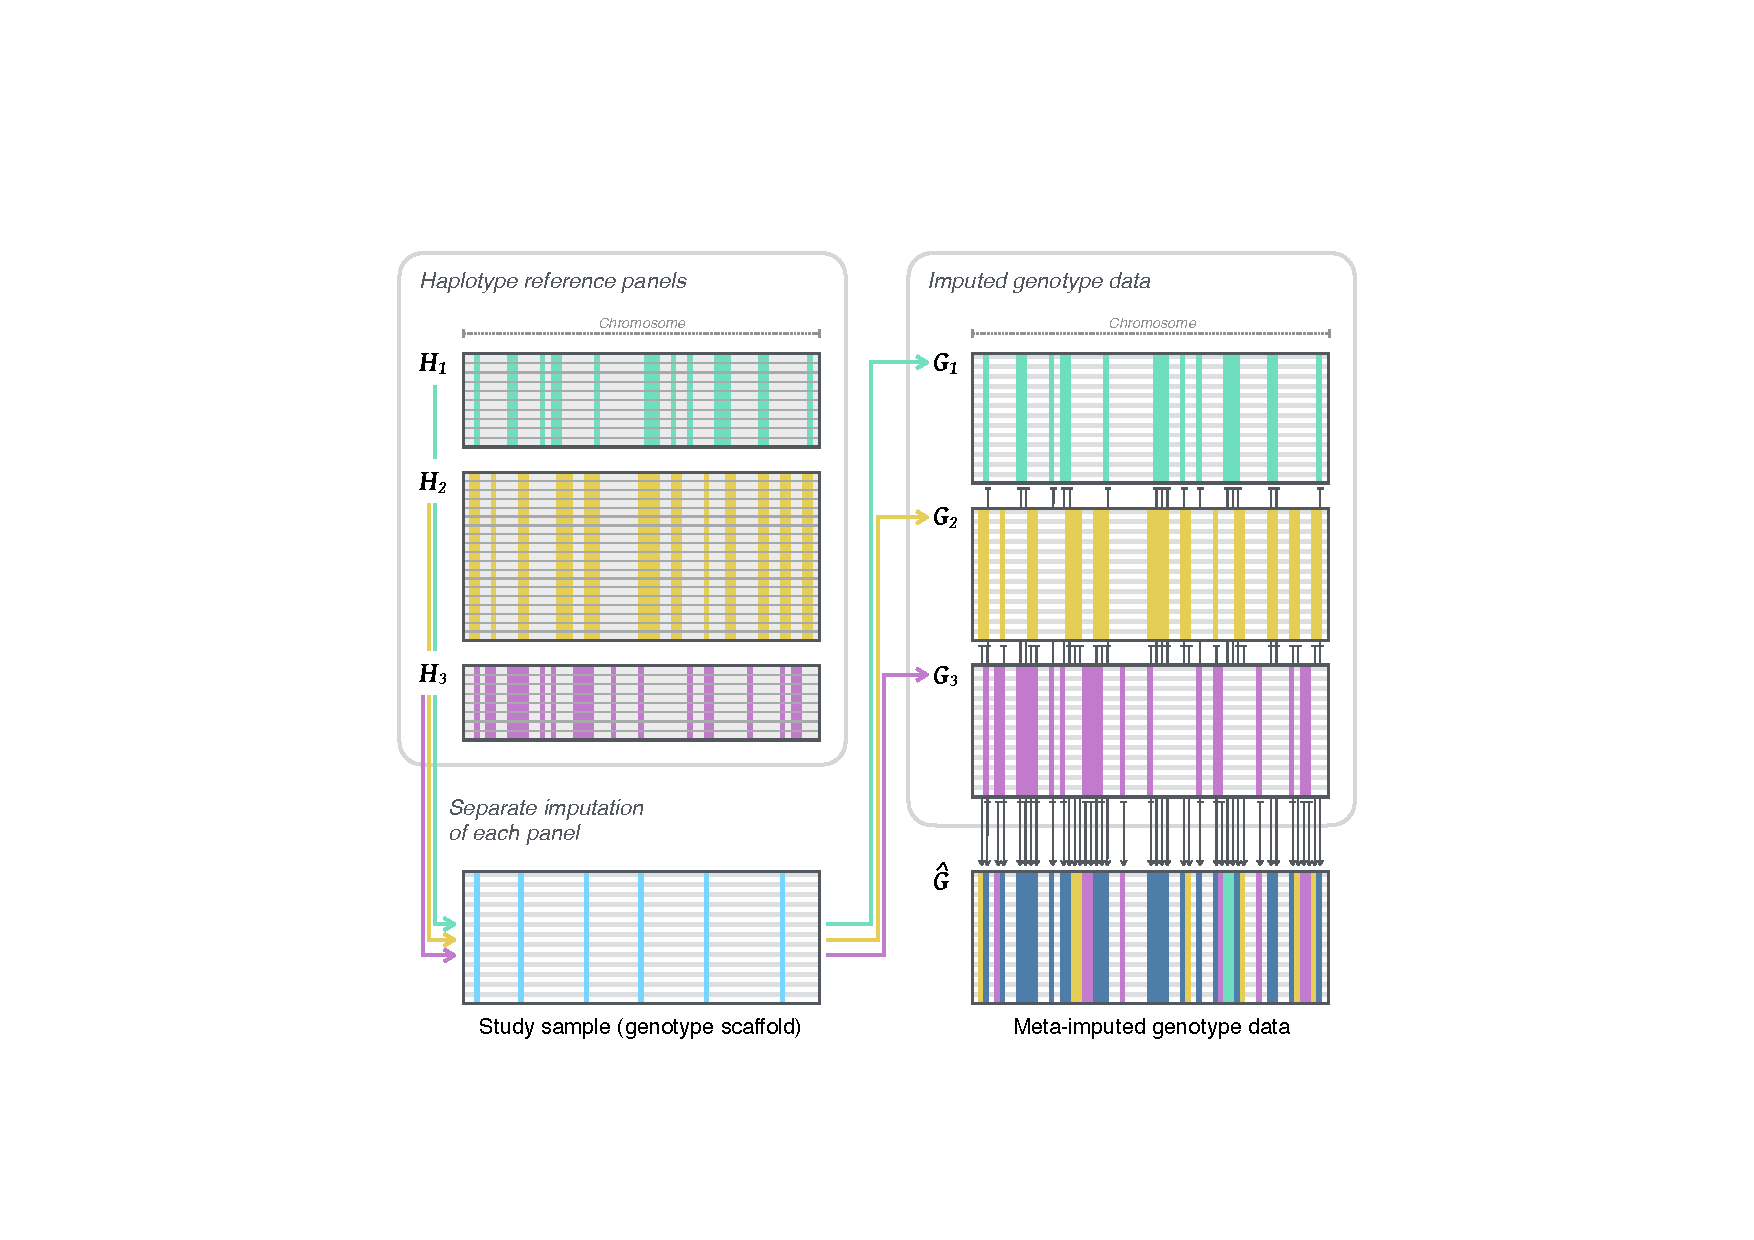
\includegraphics[width=\textwidth]{./img/ch2/info_algorithm}
\Caption{Illustration of the meta-imputation concept}
{An example of \n{3} haplotype reference panels is shown; denoted by $H_1$, $H_2$, and $H_3$, where haplotypes are indicated by row (\emph{grey}) and observed variant sites are indicated by column.
Each panel may vary in sample size and coverage.
Reference data are separately imputed into the same study sample, which is a ``scaffold'' of typed genotype markers, where individual genotypes are indicated by row (alternating \emph{grey-white}) and observed markers by column (\emph{light-blue}).
Each imputation returns an imputed genotype dataset, denoted by $G_1$, $G_2$, and $G_3$, containing marker genotypes as present in the corresponding reference panel, but where the number of individuals, $N$, is the same as in the study sample in each imputed dataset.
Imputed data are combined through meta-imputation, such that the resulting genotype dataset, $\hat{G}$, contains the union of variant sites across panels.
Variants merged across multiple datasets are indicated (\emph{dark-blue}); the markers specific to a given panel are indicated by their corresponding colour.}
{fig:info_algorithm}
\end{figure}

%

Meta-imputation combines available genotype matrices in an aggregated matrix, $A$, of size ${M_{A} \times N \times L}$ where $M_{A}$ is the number of variants in the combined set of sites across imputed panels.
The algorithm merges genotype information at overlapping variants by gathering those that correspond to the same genomic position per chromosome.
Here, the word \emph{analogue} is used to refer to the set of available data vectors that correspond to the same variant.
Let $a_{i}$ denote an analogue variant, \ie the set of overlapping genotype vectors at the $i\text{th}$ site in the aggregated matrix, and $a_{ij}$ an analogue genotype, \ie the set of  overlapping genotypes at this site in individual~$j$.
Note that the number of genotypes referred to by $a_{ij}$ may vary dependent on presence in the reference panel.
Let $l$ denote the number of overlapping variants in an analogue, where ${1 \leq l \leq L}$, such that $l_i$ refers to the size of $a_i$.

Genotype formats may differ according to the type of data available.
Note that the following considers \glspl{snp} specifically.
In generic terms, a genotype can be observed in one of \n{3} possible states; homozygous for the reference allele, heterozygous, or homozygous for the alternate allele, which can be encoded by the alternate allele count (\emph{allele dosage}); that is $0$, $1$, or $2$, respectively.
Imputed genotypes are typically expressed by the uncertainty associated with the imputation process.
Here, an imputed genotype is considered as a tuple (${p_{0}}$, ${p_{1}}$, ${p_{2}}$) of sum 1, representing the inferred posterior probability per genotypic state.
Hence, $a_{ijk}$ refers to a genotype tuple at the $i\text{th}$~site in individual~$j$ taken from $G_{k}$.

The meta-imputation algorithm assigns a score value, $s_{ijk}$, to each $a_{ijk}$; \ie each candidate genotype per analogue variant.
A \emph{meta-imputed} genotype is formed, denoted by $\hat{g}_{ij}$, by merging candidate genotype data conditional on the score assigned.
At sites where ${l_{i}=1}$, that is a given variant was imputed from only \n{1} reference panel, genotype data are retained as is, to capture as much variation as available from each separate imputation.
The resulting genotype matrix, $\hat{G}$, contains the union of variants across input datasets.
A simplified illustration of the meta-imputation concept is given in \cpref{fig:info_algorithm}.



%
\subsection{Score metrics}
\label{metaimpute_score}
%

The score metrics considered in this work are described below; asserted 2-letter codes are used for the remainder of this chapter.

\paragraph{Maximum probability (\texttt{MP}).}
The mode of the probability distribution of a candidate genotype is taken as the value of the genotype's score; that is the maximum value in the tuple of posterior probabilities, which takes values in ${[0,1]}$.
The score is separately obtained for each candidate genotype, $a_{ijk}$, such that
\begin{equation}
	s_{ijk} ~=~ \max\left[(p_0,p_1,p_2)_{ijk}\right]\ .
\end{equation}

\paragraph{\texttt{IMPUTE2} information score (\texttt{IS}).}
The information score (or \emph{info-score}) is used, which is a quality metric of the difference between observed and expected information, dependent on the imputed genotype distribution and estimated allele frequency; see definition below \citep[][S3, eq.~16; modified here to correspond to present notation]{Marchini:2010cga}.
\begin{equation}
	\text{I}_{ik} ~=~
	\begin{cases}
    ~ 1 - \frac{\sum_{j=1}^{N} f_{ijk} ~ e_{ijk}^2}{2N \hat{\theta}_{ik} (1 - \hat{\theta}_{ik})} &
		~ \text{if} ~
		\hat{\theta}_{ik} \in (0,1) \\
    ~ 1 & ~ \text{if} ~ \hat{\theta}_{ik} = 0, \hat{\theta}_{ik} = 1
  \end{cases}
\end{equation}
where ${e_{ijk} = {p_{1}}_{ijk} + 2 {p_{2}}_{ijk}}$ is the expected allele dosage, similarly ${f_{ijk} = {p_{1}}_{ijk} + 4 {p_{2}}_{ijk}}$, and $\hat{\theta}_{ik}$ is an estimate of the unknown population allele frequency, calculated as
\begin{equation}
	\hat{\theta}_{ik} ~=~ \frac{\sum_{j=1}^{N} e_{ijk}}{2N}\ .
\end{equation}
The \texttt{IMPUTE2} info-score takes values in $\lbrack 0,1 \rbrack$ where values close to $0$~or~$1$ indicate low or high certainty, respectively.
This and other information measures (\eg \texttt{Beagle}~$R^{2}$ or \texttt{Mach}~$\hat r^{2}$) are commonly used as a filter criterion in \gls{qc} of imputed \gls{gwa} data.
Because meta-imputation was evaluated using \texttt{IMPUTE2} for imputations (see \ccref{sec:meta_methods_imp}), it is justifiable to use this information measure as a score metric.
Since the info-score is calculated per imputed variant, the same score value is assigned to each candidate genotype imputed from a given reference panel at each site.
Its value is assigned to each candidate genotype at a given imputed variant; that is
\begin{equation}
	s_{ijk} ~=~ \text{I}_{ik} ~\forall j \ .
\end{equation}

\paragraph{Sample certainty (\texttt{SC}).}
A simple measure of imputation certainty is calculated per individual, such that a score value is assigned to genotypes across variants.
This metric is calculated as the proportion of an individual's genotypes which have a maximum probability that satisfies a threshold rule, defined as
\begin{equation}
	s_{ijk} ~=~ \frac{\sum_{i=1}^{M} \text{I}_{ijk}}{M}
\end{equation}
where
\begin{equation}
	\text{I}_{ijk} ~=~
	\begin{cases}
    ~ 1 & ~ \text{if} ~ \max\left[(p_0,p_1,p_2)_{ijk}\right] \geq r\\
    ~ 0 & ~ \text{otherwise}
  \end{cases}
\end{equation}
where $r$ is an arbitrarily defined value.
In the present implementation, this threshold was set to ${r=0.9}$.
The intention of the \texttt{SC} metric is to prioritise imputations from reference haplotypes which show a closer fit to the genetic variation observed per individual in the study sample, which is assumed to be captured by the posterior probability at imputed genotypes.
It must be noted that more sophisticated approaches for the estimation of genetic similarity exist, which provide summary statistics that could be used in place of the present score metric.
Possible examples range from multi-locus statistics to fine-scale measures of population structure and demographic history \citep[\eg][]{McVean:2004ca, Lawson:2012ha}.

\paragraph{Random score (\texttt{RS}).}
In addition, the option to assign random score values to candidate genotypes was included, to be considered as a control against which the above metrics were compared.
The score was explicitly calculated as
\begin{equation}
	s_{ijk} ~=~ \frac{\operatorname{rand}(R)}{100}\ , ~\quad~ R \in \{ 1,2,\ldots, 99 \}
\end{equation}
where $\operatorname{rand}{(\cdot)}$ is a function which uniformly selects \n{1} value from $R$ at random, such that ${0 < s_{ijk} < 1}$.


%
\subsection{Merge operations}
\label{metaimpute_merge}
%

Any operation to merge the information available per analogue genotype can be divided into \n{1} of \n{2} conceptually distinct approaches; either one candidate genotype is selected and others are discarded, or a new genotype tuple is mathematically derived from available data.
Accordingly, I considered the following \n{2} operations; note that the specified 3-letter codes are used henceforth.

\paragraph{Maximum score selection (\texttt{MSS}).}
A candidate genotype is selected by using score metrics as a ranking criterion, where the genotype tuple with the highest assigned score is selected from an analogue genotype in $a_{ij}$ and retained as is in $\hat{g}_{ij}$; see below.
\begin{equation}
	\hat{k} ~=~ \argmax_{k \in \{ 1,\ldots,l_i \}} \left[ s_{ij} \right]
	~ \quad ~ \textbf{s.t.} ~ \quad ~
	\hat{g}_{ij} ~=~ a_{ij\hat{k}}
\end{equation}
If the highest score value is equal in more than \n{1} candidate genotypes, \n{1} is selected at random from those with the highest score.

\paragraph{Weighted linear combination (\texttt{WLS}).}
Tuple values of the meta-imputed genotype are derived from candidate genotypes as a linear combination of their posterior probability per genotypic state.
This is calculated as the weighted average over analogue genotype probabilities, using corresponding score values as weights.
Each candidate genotype thereby contributes to the resulting probability distribution in $\hat{g}_{ij}$\Delete{, except for genotypes with $s_{ijk}=0$}.
Probability values in each tuple $a_{ijk}$ are multiplied by their assigned $s_{ijk}$ after normalising scores such that values in $s_{ij}$ sum to 1.
The tuple of the meta-imputed genotype is then constructed by calculating the sum over the weighted probabilities at each genotypic state; see below (the mathematical definition follows \citet{Stone:1961js}).
\begin{equation}\label{metaimpute_wlc}
\hat{g}_{ij} ~=~ {\left( \hat{p}_{0}, \hat{p}_{1}, \hat{p}_{2} \right)}_{ij} ~=~
\sum_{k = 1}^{l_i}  {\left( p_{0}, p_{1}, p_{2} \right)}_{ijk} ~ s_{ijk}
\end{equation}
Implicitly, the resulting probability distribution in $\hat{g}_{ij}$ sums to~1.
In contrast to \texttt{MSS} above, the weighted linear combination of genotype data does not discard available information.
But note that tuple values may not be regarded as posterior probabilities when candidate genotypes were combined using \texttt{WLS}, but rather as ``pseudo-probabilities''.



%
\section{Generation of reference datasets}
\label{metaimpute_data}
%

Multiple reference panels were derived from the \glsentryfull{1kg} Phase~\rom{1} dataset, which comprises both low-coverage \glsentrylong{wgs} and \glsentrylong{wes} data of \n{1092} individuals from \n{14}~populations of European, East-Asian, African, and admixed American ancestries.\footnote{Note that I completed work on the \emph{meta-imputation} project prior to the release of \gls{1kg} Phase~\rom{3} \citep{Auton:2015gk}.}
This original dataset was split into non-overlapping subsets in \n{2} scenarios, A and B, reflecting situations when reference data of similar or distinct ethnic backgrounds would be available for imputation into a given study sample; see details below.
\begin{description}
	\item[\textbf{Scenario A}] included \n{4} panels composed of individuals belonging to European sub-populations (CEU, FIN, GBR, and TSI) as an example use case when different reference data of similar ethnic background are available.
	\item[\textbf{Scenario B}] included \n{4} panels from different continental populations (AFR, AMR, ASN, and EUR) as an example use case when panels of distinct-ancestry samples are available.
\end{description}
Because sample sizes of the population groups considered in Scenario~B differed in \gls{1kg} (more than in Scenario~A), extracted individuals were randomly drawn from each group to create panels of equal size.
\Addition{Note that this was done to be able to better compare imputation accuracy among the generated panels, but which is not a requirement when using the meta-imputation method.}
Monomorphic sites and singletons were removed in each generated panel to more closely resemble data from independently conducted studies, where singleton or monomorphic variant calls are likely to be removed in the final dataset.
In the following, the term \emph{split panel} is used to denote subset reference data from \gls{1kg}.
Throughout, analyses were limited to data from \n{1} chromosome, namely chromosome~20.
This was done to allow for a larger number of replicate analyses, as will be described in \cpref{sec:metaimpute_power}.


%
% !TEX root = ../../main.tex


\begin{figure}[!htb]
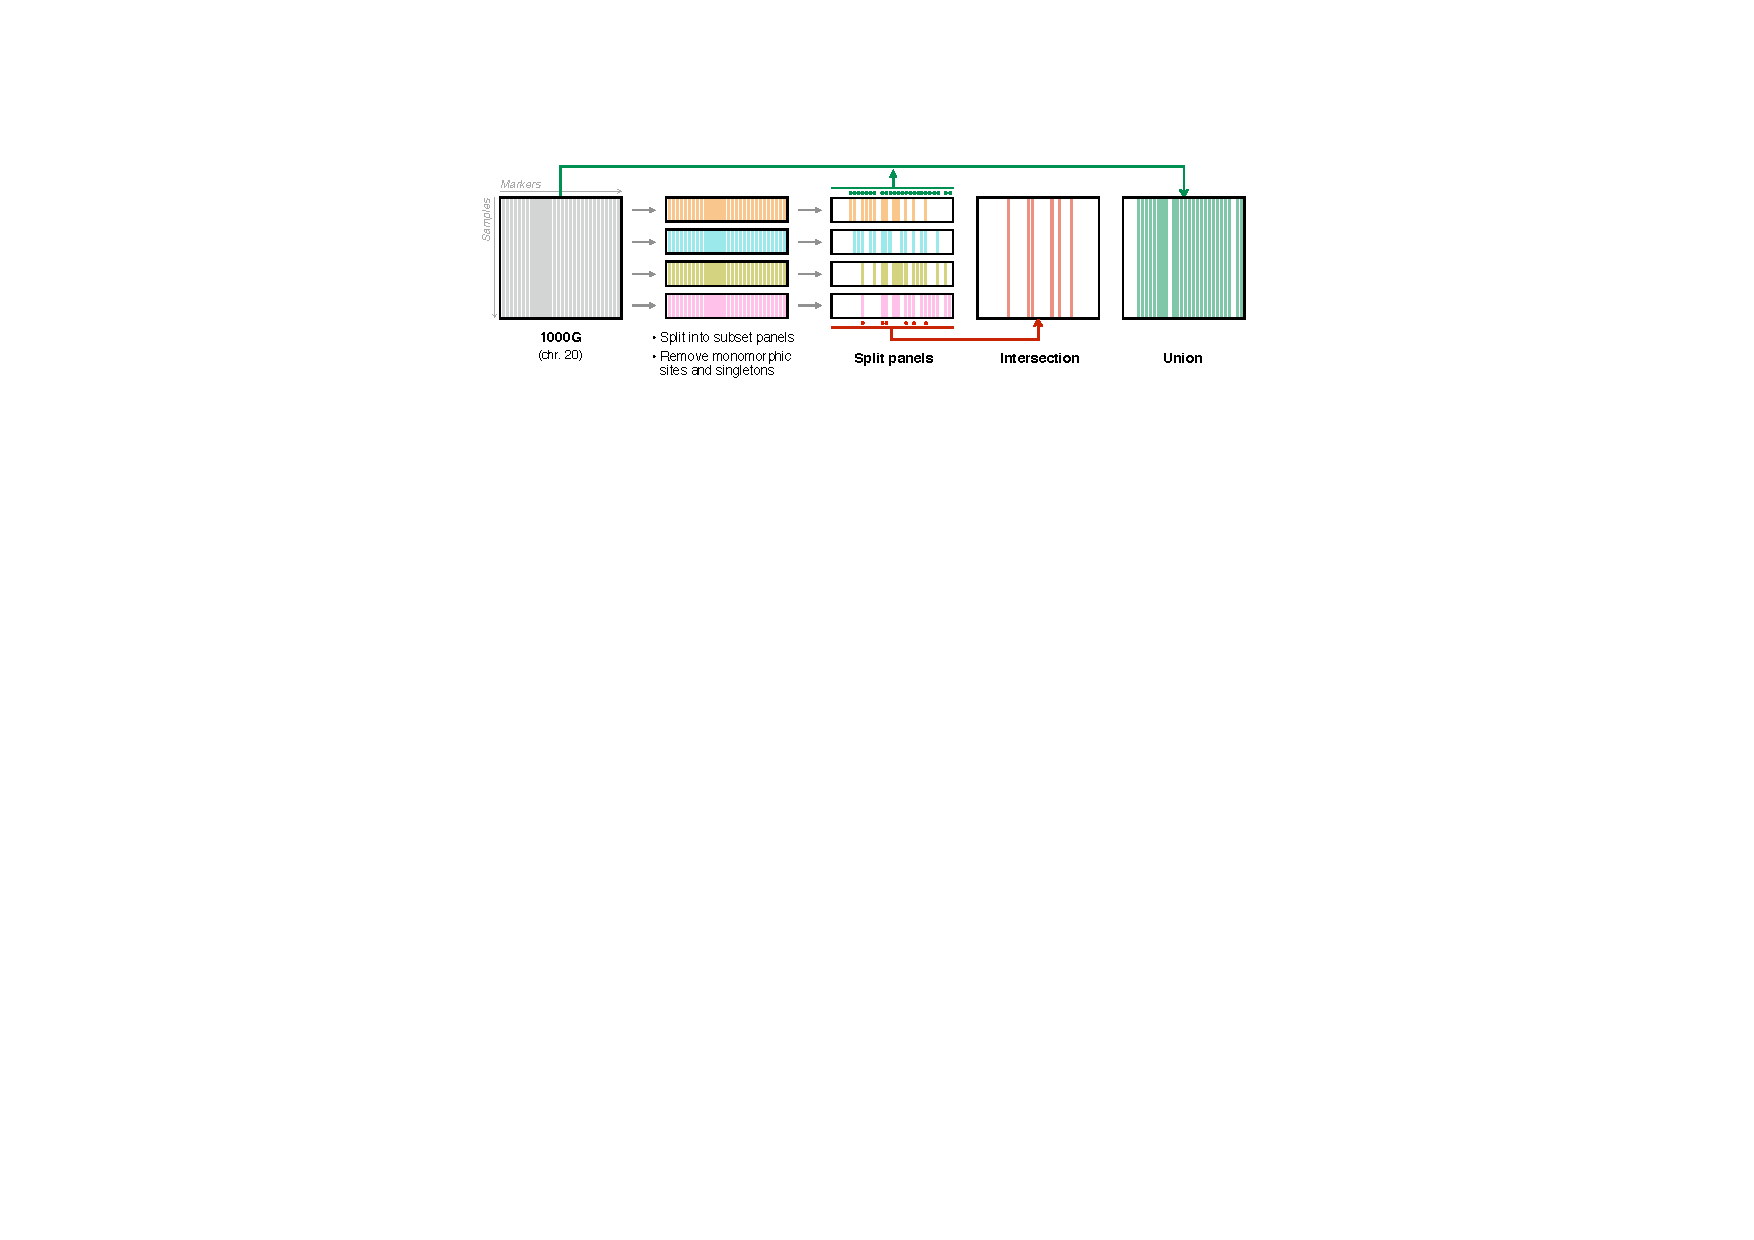
\includegraphics[width=\textwidth]{./img/ch2/info_design_panels}
\Caption{Generation of reference panels in each scenario}
{The original 1000 Genomes dataset (Phase~\rom{1}, chromosome~20) was used to generate multiple, smaller panels for imputation.
This was done in \n{2} scenarios to create data of similar or distinct ethnic backgrounds.
In each scenario, data were split into \n{4} \emph{split} panels of approximately equal size.
Monomorphic sites and singletons were removed in each split panel.
\N{2} additional panels were generated from the obtained split panels per scenario;
\n{1} \emph{intersection} panel and \n{1} \emph{union} panel, both of which contained the union of individuals across split panels, but where the intersection panel only included sites if captured in all split panels, and the union panel included all sites as observed in the original dataset (except monomorphic or singleton sites as per the individuals included).}
{fig:info_design_panels}
\end{figure}

%

Generated split panels were used for separate imputations and subsequent integration of estimated genotype data through meta-imputation.
To compare meta-imputed genotypes to those that were directly imputed from a unified panel, \n{2} additional reference datasets were generated from \gls{1kg} per scenario, which combined samples across respective split panels; referred to as the \emph{intersection} panel and the \emph{union} panel.
The union reference contained variation as present in the original dataset, but for the individuals contained across split panels in a given scenario, and with monomorphic and singleton variants removed.
The intersection reference contained the same set of individuals as the union panel, but where variant sites not shared across all split panels were removed.
Unlike the split panels, from which imputed data were combined in meta-imputation, the genotype datasets obtained in imputations from the intersection and union panels were used in direct comparisons to meta-imputed data.
The process of reference data generation is illustrated in \cpref{fig:info_design_panels}.
A summary of the final reference datasets in each scenario is given in \cpref{tab:refsize}.

%
% !TEX root = ../../main.tex


\begin{table}[!htb]
\Caption{Dimensions of generated reference data used for imputations}
{Panels included in Scenarios~A~and~B were generated from the \gls{1kg} Phase~\rom{1} dataset.
These ``split'' panels are named after their respective population codes in \gls{1kg}.
Only data from chromosome~20 were considered.
Note that split panels in Scenario~B were reduced to match the size of the smallest panel in that scenario.
Both the \emph{intersection} and the \emph{union} panels were created from the combined set of individuals across panels in each scenario.}
{tab:refsize}
\centering
\begin{tabular}{%
	lS[table-format=3.0]S[table-format=6.0]%
	c
	lS[table-format=3.0]S[table-format=6.0]%
	}
\toprule
\multicolumn{3}{c}{Scenario A} & & \multicolumn{3}{c}{Scenario B} \\
\cmidrule(lr){1-3}
\cmidrule(lr){5-7}
{Panel} & {Samples} & {Variants}  & &  {Panel} & {Samples} & {Variants} \\
\otoprule
\textsl{CEU} &  85 & 197252 & &  \textsl{AFR} & 181 & 429088  \\
\textsl{FIN} &  93 & 205093 & &  \textsl{AMR} & 181 & 307454  \\
\textsl{GBR} &  89 & 202707 & &  \textsl{ASN} & 181 & 209209  \\
\textsl{TSI} &  98 & 207583 & &  \textsl{EUR} & 181 & 233527  \\
\cmidrule(lr){1-3}
\cmidrule(lr){5-7}
Intersection & 365 & 168744  & &  Intersection & 724 & 144259  \\
Union        & 365 & 253852  & &  Union        & 724 & 559172  \\
\bottomrule
\end{tabular}
\end{table}

%


%
\section{Accuracy of estimated genotypes}
\label{metaimpute_accuracy}
%

Evaluation of genotype accuracy was done in \n{2} parts.
First, each combination of score metric and merge operation was tested and compared to select the best performing setting for downstream analyses.
Second, meta-imputed genotypes generated under the selected setting were examined in comparison to genotype data imputed from each split reference panel, as well as the intersection and union imputations.
Details about the methods used are given in the section below.
Results are presented in \cpref{metaimpute_accuracy_results}.



%
\subsection{Methods}
\label{sec:meta_accuracy_methods}
%

Calculation of genotype accuracy requires that the true genotypic states at untyped variants in a study sample are known.
This was done by using a larger dataset from which a subset of variants was drawn to form an imputation scaffold.
Missing variants were then re-imputed from available reference panels.
The generation of the genotype scaffold is described below, followed by details about imputation, quality control, and the calculation of genotype accuracy.


%
\subsubsection{Generation of genotype scaffold data (study sample)}
%

The study sample used for imputations was extracted as a scaffold from data of the \gls{got2d}, consisting of \n{2657} individuals of Central and Northern European descent \citep{Fuchsberger:2016df}.\footnote{GoT2D Consortium: \url{http://www.type2diabetesgenetics.org/projects/got2d} \accessed{2016}{12}{02}}
The dataset is composed of data obtained on several platforms; \Addition{low-coverage} \glsentrylong{wgs} \Addition{($\sim5\times$)}, \Addition{high-coverage} \glsentrylong{wes} \Addition{($\sim82\times$)}, and genotyping data using the \emph{Illumina Omni2.5 Array}.
To maintain a congruent set of markers in the genotype scaffold, variants typed on the latter were extracted from the larger \gls{got2d} dataset, yielding \n{40255} variants of in total \n{387499} \glspl{snp} on chromosome~20 in \gls{got2d}, after removing monomorphic sites and singletons.
Remaining sites were masked for comparison after imputation, where imputed variants were matched to their corresponding sites in the masked dataset to calculate genotype accuracy.

%
% !TEX root = ../../main.tex


\begin{figure}[!htb]
\centering
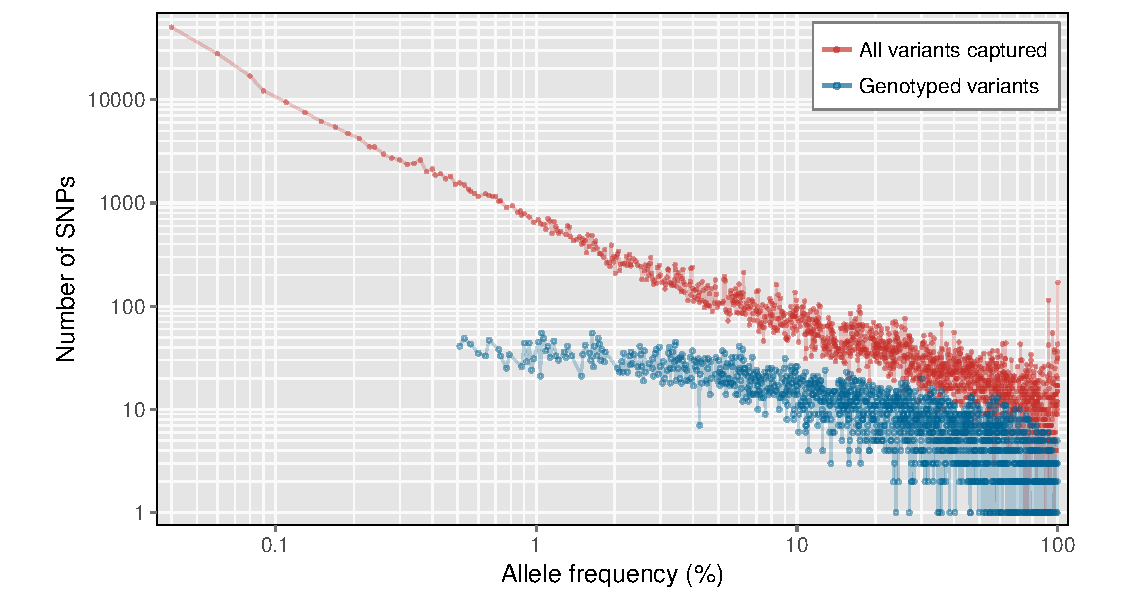
\includegraphics[width=0.9\textwidth]{./img/ch2/sfs_got2d}
\Caption{Site frequency spectrum of variants captured in GoT2D (chromosome 20)}
{The \glsentryfull{sfs} is shown for SNPs as captured in the full \gls{got2d} dataset (\emph{red}) and SNPs genotyped using \emph{Illumina Omni2.5 Array} (\emph{blue}), given the allele frequencies observed in the full \gls{got2d} sample for chromosome~20, after removing singletons and monomorphic sites.}
{fig:sfs_got2d}
\end{figure}

%

\Addition{\Cpref{fig:sfs_got2d} shows the \gls{sfs} of variants captured in the \gls{got2d} dataset, highlighting the discrepancy between the frequency distribution observed at all captured variants and those obtained through genotyping only.
Rare variants (\eg at allele frequency $\leq1\%$) are underrepresented in the genotyped set of SNPs and, thus, in the extracted genotype scaffold.
Imputation from a reference panel into the scaffold attempts to fill these gaps, including sites with alleles occurring at lower frequencies.}


%
\subsubsection{Imputation and quality control}
\label{sec:meta_methods_imp}
%

Imputations were performed using \texttt{IMPUTE2} version~2.3.0 \citep{Howie:2009hq}, and executed in consecutive chunks of 5~\glspl{Mb}.
The \gls{got2d} dataset comprises already phased haplotypes, so imputations were carried out on pre-phased genotypes (command line argument \verb|-use_prephased_g| in \texttt{IMPUTE2}).
Because meta-imputation is indirectly based on information from more reference haplotypes than available in each separate imputation, the number of haplotypes that inform the imputation process was set to the maximum number present in a given reference panel (command line argument \verb|-k_hap| in \texttt{IMPUTE2}).
This was done to minimise potential biases in comparisons between meta-imputed and imputed genotypes, but is not a requirement for general applications of this approach.

%
% !TEX root = ../../main.tex


\begin{figure}[!htb]
\centering
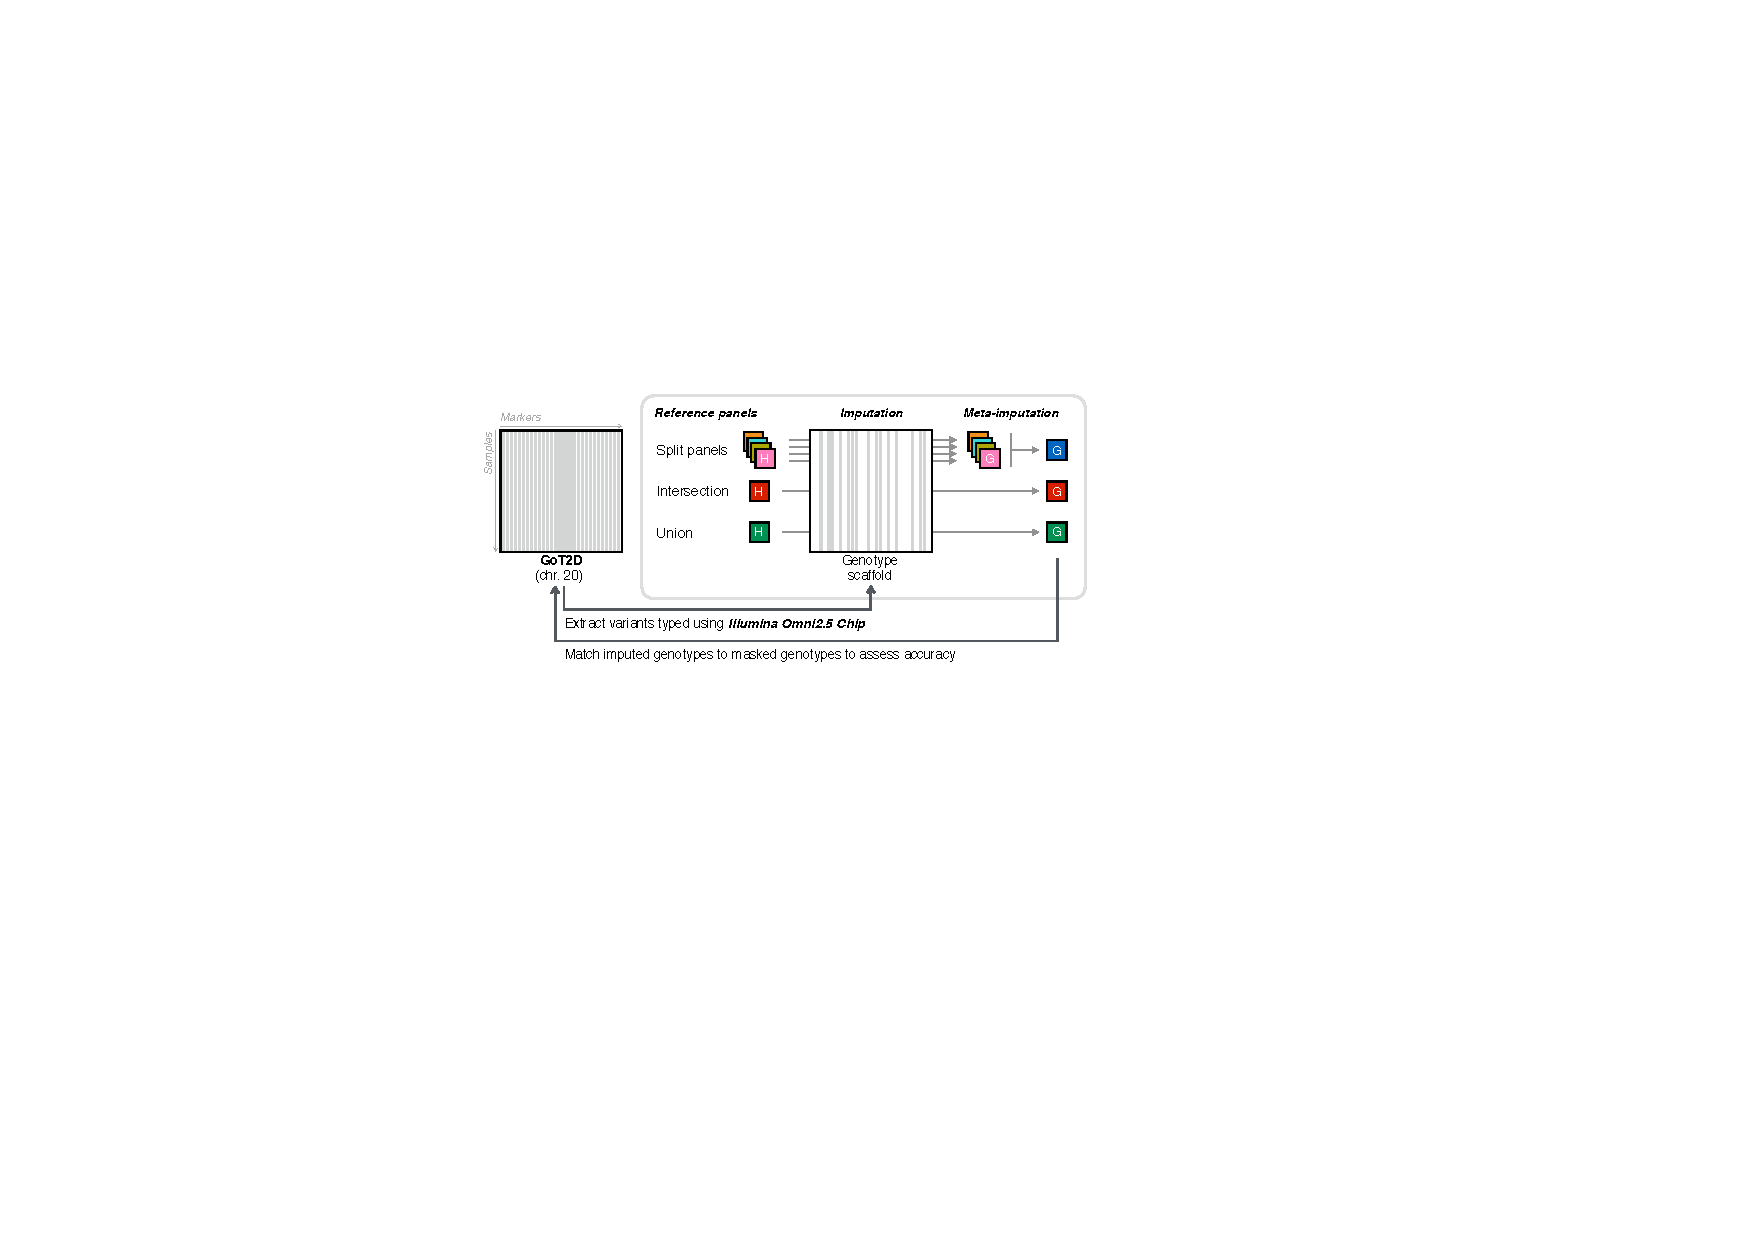
\includegraphics[width=0.9\textwidth]{./img/ch2/info_design_accuracy}
\Caption{Illustration of the accuracy assessment process}
{Imputations were performed on the same genotype scaffold, which consisted of genetic markers obtained through genotyping using \emph{Illumina Omni2.5 Chip}, which was part of the \gls{got2d} dataset.
This scaffold was extracted from \gls{got2d} data, where remaining markers were masked for subsequent calculation of accuracy (squared Pearson correlation coefficient, $r^2$) at corresponding sites after imputation.
Several reference panels were available, which were imputed into the same scaffold.
Meta-imputation was applied to the imputed datasets obtained from split panels, which were generated as distinct subsets from the \gls{1kg} dataset.
The intersection and union panels were separately imputed into the scaffold and subsequently compared to meta-imputed data on corresponding variant sets.}
{fig:info_design_accuracy}
\end{figure}

%

Imputed and meta-imputed genotype data were filtered in \gls{qc}, removing variants at \texttt{IMPUTE2} ${\mbox{info-score}<0.4}$ and at deviations from \gls{hwe} at ${\pvalue<\num{1e-4}}$.
\Addition{These metrics were computed using \texttt{QCTOOL},\footnote{\texttt{QCTOOL}: \url{http://www.well.ox.ac.uk/~gav/qctool} \accessed{2016}{12}{02}} which was performed on both directly imputed and meta-imputed datasets.}
Imputed data were filtered before the assessment of imputation accuracy, but not before integration through meta-imputation.
The proportion of variants retained after \gls{qc} was used as an indicator for data quality in comparisons between imputed and meta-imputed data, \Addition{as well as to characterise the quality achieved though using different meta-imputation settings.}
Hence, \gls{qc} results were separately reported for each part of the analysis.
A summary of the described analysis is illustrated in \cpref{fig:info_design_accuracy}.



\subsubsection{Calculation of genotype accuracy}

Genotype accuracy was calculated as the squared Pearson correlation coefficient, $r^2$, as a measure for the strength of the linear relationship between imputed and masked genotype vectors, such that $r^2$ was computed per site.
This was done after conversion of genotypes to allelic dosage, calculated as ${d=0p_{0}+1p_{1}+2p_{2}}$ where ${d \in \lbrace 0,1,2 \rbrace}$ for masked genotypes or ${0 \leq d \leq 2}$ when calculated from imputed genotype probabilities.
Note that the Pearson correlation coefficient is defined as the covariance divided by the product of the standard deviation (SD) of \n{2} random variables.
This is problematic if $\text{SD}=0$, which is the case when variant genotypes are imputed as being monomorphic.
To compensate for this loss in precision towards lower frequencies, the coefficient was set to ${r^2=0}$ for monomorphic variants.
Imputed and masked genotype data were sorted into \gls{maf} bins, based on their population frequency (\gls{maf} in the \gls{got2d} dataset).
In the following, accuracy is reported as mean~$r^2$ calculated at corresponding variants per \gls{maf} bin.


%
\subsection{Results}
\label{metaimpute_accuracy_results}
%

Accuracy of meta-imputed genotypes was explored for each combination of score metric and merge operation.
The best performing setting was then chosen for comparison to direct imputations, as well as further analysis in \cpref{sec:metaimpute_power}.

\subsubsection{Comparison of meta-imputation settings}

Each combination of score metric and merge operation produced an identical set of variants; that is, the combined set of variants across imputed panels.
In total, \num{253852} variants were returned from each meta-imputation in Scenario~A (European sub-populations) and \num{559172} in Scenario~B (continental populations); \ie the same number as captured by the union panel.
Meta-imputed datasets were further reduced to the set of variants that matched to masked variants in the original \gls{got2d} dataset.
Variants contained in the genotype scaffold were removed, as these were not imputed.
This retained \num{181561} and \num{196300} variants in Scenarios~A and B, respectively.

\Addition{First, I report the impact of \glsentryfull{qc} to characterise the different meta-imputation settings by the number of retained sites.
Briefly, recall that \gls{qc} was carried out to remove variant sites at \texttt{IMPUTE2} ${\mbox{info-score}<0.4}$ and at deviations from \gls{hwe} at ${\pvalue<\num{1e-4}}$.
I then report genotype accuracy measured on sites retained after \gls{qc} for each setting.}


%
% !TEX root = ../../main.tex


\begin{table}[!htb]
\TableUnits
\Caption{Variants retained after quality control per meta-imputation setting}
{\DefaultUnits
The number of variants retained after \glsentryfull{qc}, $n$, per meta-imputation setting (combination of score metric and merge operation) in Scenario~A and B.
The percentage is given relative to the set of sites matched to masked variants in the \gls{got2d} dataset and after removing sites contained in the imputation scaffold;
\num{181561} and \num{196300} in A and B, respectively.
Variants were removed at \texttt{IMPUTE2} ${\text{info-score} < 0.4}$ and at deviations from \gls{hwe} at ${\text{p-value} < \num{1e-4}}$.}
{tab:mim_qc}
\centering
\begin{tabular}{%
	cc%
	S[table-format=6.0]%
	@{\quad}S[round-precision=1,table-format=1.1]%
	S[table-format=6.0]%
	@{\quad}S[round-precision=1,table-format=1.1]%
	}
\toprule
{Merge} & {Score} &
\multicolumn{2}{c}{Scenario A} &
\multicolumn{2}{c}{Scenario B} \\
\cmidrule(lr){3-4}
\cmidrule(lr){5-6}
 & & {$n$ retained} & {(\%)}  & {$n$ retained} & {(\%)} \\
\otoprule
\texttt{MSS}
& \texttt{MP}  &  168595 & (92.85860)  &  178034 & (90.69485) \\
& \texttt{IS}  &  169455 & (93.33227)  &  179677 & (91.53184) \\
& \texttt{SC}  &  168686 & (92.90872)  &  179449 & (91.41569) \\
& \texttt{RS}  &  165877 & (91.36158)  &  171517 & (87.37494) \\
\cmidrule(lr){2-6}
\texttt{WLC}
& \texttt{MP}  &  161079 & (88.71894)  &  166458 & (84.79776) \\
& \texttt{IS}  &  162511 & (89.50766)  &  169860 & (86.53082) \\
& \texttt{SC}  &  160464 & (88.38021)  &  165907 & (84.51707) \\
& \texttt{RS}  &  160369 & (88.32789)  &  165787 & (84.45593) \\
 \bottomrule
 \end{tabular}
\end{table}

%

The number of variants retained after \gls{qc} differed among meta-imputation settings; see \cpref{tab:mim_qc}.
Merge operations had a higher impact on the quality of meta-imputed genotypes than score metrics.
In Scenario~A, on average \MeanPercent{92.61529}{0.4311945} of variants were retained when \texttt{MSS} (maximum score selection) was used as the merge operation, with fewer retained using \texttt{WLC} (weighted linear combination), where \MeanPercent{88.73368}{0.2721617} were retained on average.
This was similar in Scenario~B, where \MeanPercent{90.25433}{0.9774864} and \MeanPercent{85.07539}{0.4908162}
were retained on average under \texttt{MSS} and \texttt{WLC}, respectively.
Most of the variants removed in either setting were low in frequency.
For instance at ${\text{MAF} \leq 1\%}$,
\MeanPercent{74.58665}{0.704543} and
\MeanPercent{68.25875}{0.495304} passed \gls{qc} in Scenario~A
when using \texttt{MSS} and \texttt{WLC}, respectively, as well as
\MeanPercent{72.15974}{1.730208} and
\MeanPercent{61.67898}{0.961795} in Scenario~B, respectively.
Among score metrics, the number of variants that passed \gls{qc} was lowest for \texttt{RS} (random scores) in each comparison; for example, \Percent{67.51898} and \Percent{60.53869} at ${\text{MAF} \leq 1\%}$ in A and B, respectively.

%
% !TEX root = ../../main.tex


\begin{figure}[!htb]
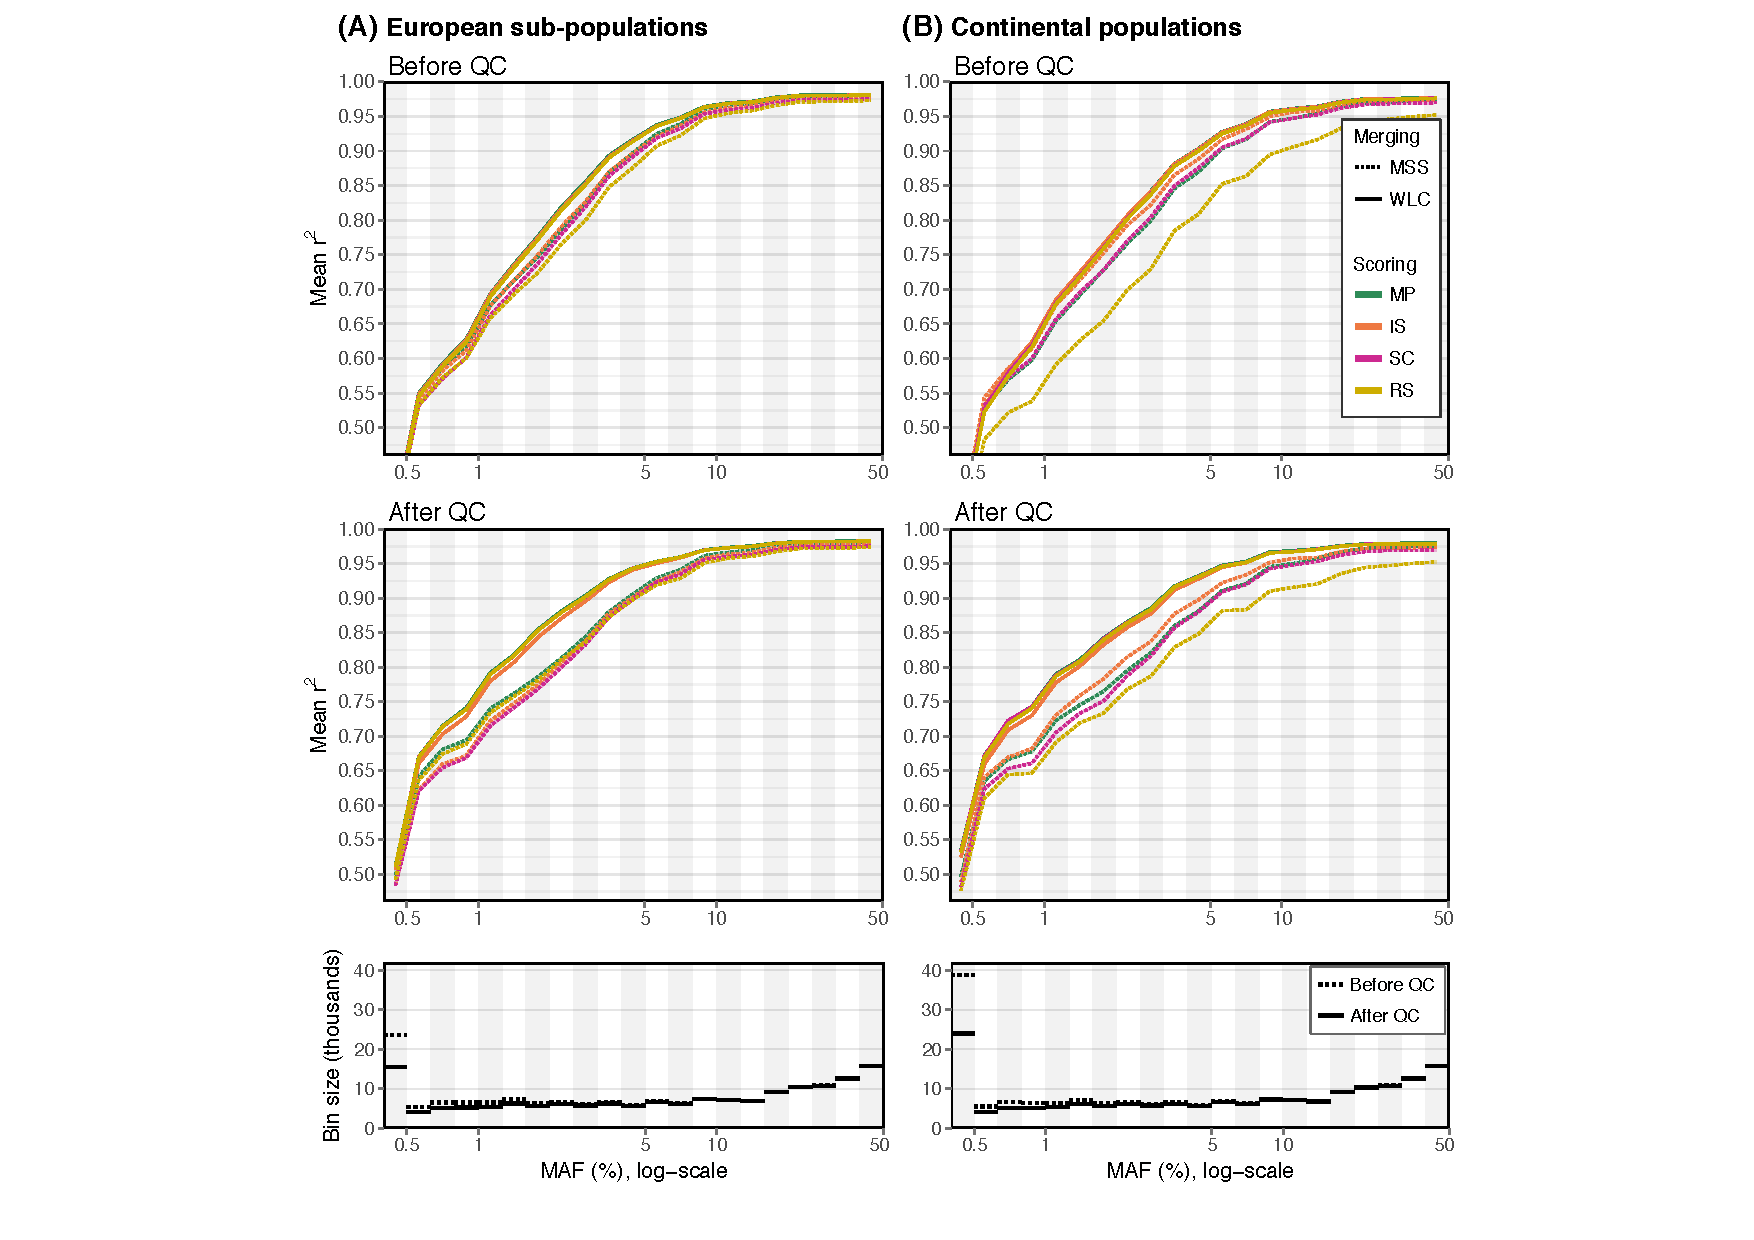
\includegraphics[width=\textwidth]{./img/ch2/accuracy_mim_maf_rsq}
\Caption{Accuracy comparison of score metrics and merge operations in meta-imputation}
{Each combination of merge operation (\texttt{MSS} and \texttt{WLC}) and score metric (\texttt{MP}, \texttt{IS}, \texttt{SC}, and \texttt{RS}) was examined in Scenarios~A and B.
Accuracy was measured as mean~${r^2}$ calculated between meta-imputed variants and variants masked in the \gls{got2d} dataset.
Results are shown both before and after \gls{qc}.
Bin sizes were defined on log-scale where \emph{grey-white} bars indicate boundaries.
The panels at the bottom indicate the number of variants per bin before \gls{qc} (\emph{dotted}) and the average number of variants per bin after \gls{qc} (\emph{solid}).}
{fig:mim_rsq}
\end{figure}

%

Although \texttt{MSS} overall preserved a relatively large proportion of markers after \gls{qc}, the accuracy of retained genotypes was overall lower compared to data produced under \texttt{WLC}.
Imputation accuracy improved after \gls{qc} as illustrated in \cpref{fig:mim_rsq}, which shows mean~$r^2$ calculated in \gls{maf} bins of equal size on log-scale.
The differences among settings were small, in particular among score metrics when \texttt{WLC} was used, but where differences in accuracy become more pronounced after \gls{qc}, which highlighted a clear distinction between merge operations.
Throughout, mean $r^2$ was higher for genotype data produced under \texttt{WLC}.
In Scenario~A, for example, mean~$r^2$ at ${\text{MAF} \leq 1\%}$ before \gls{qc} was
\MeanValue{0.4716920}{0.88645e-03} in \texttt{WLC} and
\MeanValue{0.4644852}{0.89356e-03} in \texttt{MSS}, but showed a larger difference after \gls{qc}, namely
\MeanValue{0.6049897}{1.01002e-03} and
\MeanValue{0.4716920}{0.88645e-03} in \texttt{WLC} and \texttt{MSS}, respectively.
This was also seen in Scenario~B,
where mean~$r^2$ at ${\text{MAF} \leq 1\%}$ was
\MeanValue{0.4275046}{0.79637e-03} and
\MeanValue{0.4177174}{0.81126e-03} before \gls{qc} in \texttt{WLC} and \texttt{MSS}, respectively, as well as
\MeanValue{0.5996758}{0.95121e-03} in \texttt{WLC} and
\MeanValue{0.5482575}{0.91363e-03} in \texttt{MSS} after \gls{qc}.
Accuracy differences between merge operations were more pronounced at higher \gls{maf}; as seen in \cref{fig:mim_rsq}.
For example, at ${\text{MAF} \leq 5\%}$ after \gls{qc}, mean~$r^2$ was
\MeanValue{0.8726145}{0.44164e-03} and
\MeanValue{0.8110458}{0.58041e-03}
in Scenario~A for \texttt{WLC} and \texttt{MSS}, respectively, as well as
\MeanValue{0.8617191}{0.47222e-03} and
\MeanValue{0.7931924}{0.64931e-03} in Scenario~B, respectively.

%
% !TEX root = ../../main.tex


\begin{table}[!htb]
\Caption{Accuracy measured for each meta-imputation setting}
{Accuracy was measured as mean~$r^2$ (${\pm\text{SE}}$) per \gls{maf} bin; defined to reflect average levels of accuracy measured at rare, low-frequency, and common variants.
Reported values were measured after \gls{qc} for each meta-imputation setting (combination of merge operation and score metric), in Scenarios~A and B.
\Addition{Retained variants were intersected across datasets per MAF bin.
The number of SNPs at which mean~$r^2$ was measured, $n$, is reported per scenario below the MAF range.}
The setting with the highest accuracy per \gls{maf} bin and per scenario is highlighted (\textbf{bold}).\CorrectLabel}
{tab:mim_rsq}
\centering
\TableUnits
\begin{threeparttable}
\begin{tabular}{%
	l@{\quad}c@{\quad}c%
	S[table-format=1.3]%
  @{}S[table-format=1.3]%
	S[table-format=1.3]%
	@{}S[table-format=1.3]%
	}
\toprule
{MAF bin} & {Merge} & {Score} &
\multicolumn{2}{c}{Scenario A} &
\multicolumn{2}{c}{Scenario B} \\
\cmidrule(lr){4-5}
\cmidrule(lr){6-7}
 & & & {Mean $r^2$} & {($\pm$~SE$^\ast$)} & {Mean $r^2$} & {($\pm$~SE$^\ast$)} \\
\otoprule
\multirow{3}{*}{\shortstack[l]{{\bfseries[0.00, 0.01]} \\ ~ $n_A = \num{28341}$ \\ ~ $n_B = \num{33443}$}}
 & \texttt{MSS}
  & \texttt{MP} & \bfseries 0.610644 & (2.057332)  &  0.601723 & (1.997402) \\
& & \texttt{IS} &  0.602369 & (2.067987)  &  0.599291 & (2.005439) \\
& & \texttt{SC} &  0.600145 & (2.040775)  &  0.594598 & (1.961289) \\
& & \texttt{RS} &  0.600892 & (2.051666)  &  0.578417 & (1.977409) \\
\cmidrule(lr){3-7}
& \texttt{WLC}
  & \texttt{MP} &  0.609431 & (2.041139)  & \bfseries 0.603334 & (1.957030) \\
& & \texttt{IS} &  0.607690 & (2.042573)  &  0.602691 & (1.958653) \\
& & \texttt{SC} &  0.607655 & (2.038668)  &  0.601475 & (1.951390) \\
& & \texttt{RS} &  0.607538 & (2.038956)  &  0.601114 & (1.951605) \\
\cmidrule(lr){1-7}
\multirow{3}{*}{\shortstack[l]{{\bfseries(0.01, 0.05]} \\ ~ $n_A = \num{38669}$ \\ ~ $n_B = \num{37364}$}}
 & \texttt{MSS}
  & \texttt{MP} &  0.870894 & (0.952739)  &  0.858368 & (1.075501) \\
& & \texttt{IS} &  0.859376 & (1.008176)  &  0.860007 & (1.071849) \\
& & \texttt{SC} &  0.855345 & (0.968571)  &  0.845538 & (1.061551) \\
& & \texttt{RS} &  0.847281 & (1.035284)  &  0.807120 & (1.266720) \\
\cmidrule(lr){3-7}
 & \texttt{WLC}
  & \texttt{MP} & \bfseries 0.879115 & (0.866827)  & \bfseries 0.866884 & (0.956957) \\
& & \texttt{IS} &  0.876414 & (0.877540)  &  0.865731 & (0.961977) \\
& & \texttt{SC} &  0.875809 & (0.876575)  &  0.863791 & (0.961773) \\
& & \texttt{RS} &  0.875685 & (0.876986)  &  0.863342 & (0.962887) \\
\cmidrule(lr){1-7}
\multirow{3}{*}{\shortstack[l]{{\bfseries(0.05, 0.50]} \\ ~ $n_A = \num{92797}$ \\ ~ $n_B = \num{91375}$}}
 & \texttt{MSS}
  & \texttt{MP} &  0.975080 & (0.212736)  &  0.969429 & (0.261345) \\
& & \texttt{IS} &  0.971473 & (0.232792)  &  0.970468 & (0.261916) \\
& & \texttt{SC} &  0.968808 & (0.234113)  &  0.964816 & (0.253617) \\
& & \texttt{RS} &  0.965034 & (0.262540)  &  0.939578 & (0.418136) \\
 \cmidrule(lr){3-7}
 & \texttt{WLC}
  & \texttt{MP} & \bfseries 0.977060 & (0.175426)  & \bfseries 0.973858 & (0.184269) \\
& & \texttt{IS} &  0.976379 & (0.178054)  &  0.973197 & (0.184769) \\
& & \texttt{SC} &  0.976284 & (0.178625)  &  0.972677 & (0.187366) \\
& & \texttt{RS} &  0.976253 & (0.178787)  &  0.972410 & (0.188150) \\
 \bottomrule
 \end{tabular}
 \begin{tablenotes}\footnotesize
 	\item[{${\ast}$}] Standard error (SE) $\times 10^{-3}$
 \end{tablenotes}
 \end{threeparttable}
\end{table}



%
% pre-correction (SNPS were not intersected):
%
% \begin{threeparttable}
% \begin{tabular}{%
% 	l@{\quad}c@{\quad}c%
% 	S[table-format=1.3]%
%   @{}S[table-format=1.3]%
% 	S[table-format=5.0]%
% 	S[table-format=1.3]%
% 	@{}S[table-format=1.3]%
% 	S[table-format=5.0]%
% 	}
% \toprule
% {MAF bin} & {Merge} & {Score} &
% \multicolumn{3}{c}{Scenario A} &
% \multicolumn{3}{c}{Scenario B} \\
% \cmidrule(lr){4-6}
% \cmidrule(lr){7-9}
%  & & & {Mean $r^2$} & {($\pm$~SE$^\ast$)} & {$n$} & {Mean $r^2$} & {($\pm$~SE$^\ast$)} & {$n$} \\
% \otoprule
% {{[0.00, 0.01]}}
%  & \texttt{MSS}
%    & \texttt{MP} &  0.584947 & (1.946525) & 31694  &  0.557479 & (1.822788) & 42101 \\
%  & & \texttt{IS} &  0.567338 & (1.968234) & 32099  &  0.554399 & (1.819030) & 42769 \\
%  & & \texttt{SC} &  0.564983 & (1.952322) & 31646  &  0.544109 & (1.769496) & 42335 \\
%  & & \texttt{RS} &  0.578163 & (1.988586) & 30693  &  0.535900 & (1.900744) & 38468 \\
% \cmidrule(lr){3-9}
%  & \texttt{WLC}
%    & \texttt{MP} & \bfseries 0.607540 & (2.018734) & 28818  & \bfseries 0.603224 & (1.911612) & 35020 \\
%  & & \texttt{IS} &  0.599807 & (2.003624) & 29461  &  0.592187 & (1.869955) & 37049 \\
%  & & \texttt{SC} &  0.606387 & (2.027033) & 28607  &  0.602938 & (1.910916) & 34793 \\
%  & & \texttt{RS} &  0.606362 & (2.030836) & 28545  &  0.600816 & (1.917677) & 34748 \\
% \cmidrule(lr){2-9}
% {{(0.01, 0.05]}}
%  & \texttt{MSS}
%    & \texttt{MP} &  0.818479 & (1.169141) & 43330  &  0.798540 & (1.324721) & 42865 \\
%  & & \texttt{IS} &  0.809187 & (1.168439) & 43787  &  0.813986 & (1.219665) & 43341 \\
%  & & \texttt{SC} &  0.803550 & (1.146422) & 43499  &  0.789748 & (1.231260) & 43570 \\
%  & & \texttt{RS} &  0.813084 & (1.157015) & 41848  &  0.768786 & (1.416076) & 40173 \\
% \cmidrule(lr){3-9}
%  & \texttt{WLC}
%    & \texttt{MP} & \bfseries 0.875631 & (0.870685) & 39309  & \bfseries 0.864771 & (0.936379) & 39240 \\
%  & & \texttt{IS} &  0.866544 & (0.903124) & 40107  &  0.856054 & (0.961843) & 40376 \\
%  & & \texttt{SC} &  0.874198 & (0.878352) & 39000  &  0.863396 & (0.936293) & 38992 \\
%  & & \texttt{RS} &  0.874232 & (0.878709) & 38972  &  0.862837 & (0.940820) & 38943 \\
% \cmidrule(lr){2-9}
% {{(0.05, 0.50]}}
%  & \texttt{MSS}
%  	 & \texttt{MP} &  0.970186 & (0.280056) & 93571  &  0.960115 & (0.372269) & 93068 \\
%  & & \texttt{IS} &  0.966985 & (0.287216) & 93569  &  0.962408 & (0.343832) & 93567 \\
%  & & \texttt{SC} &  0.964351 & (0.287651) & 93541  &  0.955981 & (0.342034) & 93544 \\
%  & & \texttt{RS} &  0.961725 & (0.301301) & 93336  &  0.931022 & (0.488260) & 92876 \\
%  \cmidrule(lr){3-9}
%  & \texttt{WLC}
%  	 & \texttt{MP} & \bfseries 0.976555 & (0.181332) & 92952  & \bfseries 0.972756 & (0.192585) & 92198 \\
%  & & \texttt{IS} &  0.975928 & (0.183156) & 92943  &  0.971667 & (0.195965) & 92435 \\
%  & & \texttt{SC} &  0.976184 & (0.179378) & 92857  &  0.971936 & (0.191300) & 92122 \\
%  & & \texttt{RS} &  0.976165 & (0.179460) & 92852  &  0.971744 & (0.191307) & 92096 \\
%  \bottomrule
%  \end{tabular}
%  \begin{tablenotes}\footnotesize
%  	\item[{${\ast}$}] Standard error (SE) $\times 10^{-3}$
%  \end{tablenotes}
%  \end{threeparttable}

%

Accuracy as measured for each setting after \gls{qc} is given in \cpref{tab:mim_rsq}, which shows mean~$r^2$ computed in \n{3} broader MAF bins to summarise accuracy levels at
rare variants (here defined at ${\text{MAF} \in \left[ 0.00, 0.01\right]}$),
low-frequency (${\text{MAF} \in \left( 0.01, 0.05\right]}$), and
common variants (${\text{MAF} \in \left( 0.05, 0.50\right]}$).
The \texttt{RS} score metric overall resulted in less accurate genotype data compared to other metrics, in particular in Scenario~B where \texttt{RS} was least accurate in all comparisons. This was not the case in Scenario~A, where it showed a higher accuracy than \texttt{IS} and \texttt{SC} at rare and low-frequency variants.
However, note that accuracy differences among score metrics were low overall in Scenario~A (see \cref{tab:mim_rsq}), due to the presumed higher genetic similarity between sample individuals and reference haplotypes (recall that the \gls{got2d} sample is composed of individuals of Central and Northern European descent).

Regardless, \texttt{MP} (maximum probability) outperformed other score metrics in most comparisons; except in Scenario~B, for low-frequency variants under \texttt{MSS}, where it was outperformed by \texttt{IS}.
The \texttt{MP} score metric was found to further improve accuracy under \texttt{WLC}, such that the combination of \texttt{MP} and \texttt{WLC} was seen to yield the highest accuracy in each \gls{maf} bin and in both scenarios (as highlighted in \cref{tab:mim_rsq}).
Therefore, in the following, \texttt{WLC} was chosen as merge operation and \texttt{MP} as score metric; hence, the combination of \texttt{MP} and \texttt{WLC} is implied when referring to meta-imputation below.


%
\subsubsection{Improvements of accuracy in comparison to direct imputations}
%

Available split panels were imputed into the generated study sample and imputed genotype data were then combined through meta-imputation.
The union and intersection panels were separately imputed for subsequent comparison to meta-imputed genotypes.
Before accuracy was measured, all data were subjected to \gls{qc} and variants were removed when not matched to masked variants or when contained in the imputation scaffold.
For simplicity, imputed datasets are referred to by the panel from which they were estimated.

Comparisons were based on mean~$r^2$ calculated at corresponding (meta-)imputed and masked variants pooled by \gls{maf} bin.
In addition, significant differences in the \gls{maf} distribution of imputed and corresponding meta-imputed variants were determined using the \n{2}-sample Kolmogorov–-Smirnov (KS) test.
However, significance was determined from the median of the KS test statistic, here denoted by $\widetilde{D}$, calculated at ${n = \num{500}}$ randomly selected sites over \n{1000} repeated draws.
This was done to account for varying subset sizes retained in each comparison, and to avoid potential biases due to correlations of \gls{ld} at nearby markers.
\Gls{maf} distributions were significantly different if
\begin{equation}\label{eq:meta_ks_test}
	\widetilde{D}_{n} ~ > ~ c(\alpha) \sqrt{\frac{2n}{n^2}}
\end{equation}
for significance levels ${c(0.05)=1.36}$ and ${c(0.01)=1.63}$.
A similar approach was applied by \citet{Pasaniuc:2014hq} to compare signatures of functional enrichment in imputed data.



%
% !TEX root = ../../main.tex


\begin{table}[!htb]
\TableUnits
\Caption{Effect of quality control on imputed genotype data}
{The number (percent) of variants retained after \gls{qc} for direct imputations (\ie \n{4} split panels, intersection panel, and union panel) and meta-imputation. Numbers refer to variants retained after removing unmatched sites and those contained in the imputation scaffold.}
{tab:imp_qc}
\centering
\begin{tabular}{%
	l%
	lS[table-format=6.0]@{\quad}S[round-precision=1,table-format=1.1]%
	lS[table-format=6.0]@{\quad}S[round-precision=1,table-format=1.1]%
	}
\toprule
 Panel & \multicolumn{3}{c}{Scenario A} & \multicolumn{3}{c}{Scenario B} \\
 \cmidrule(lr){2-4}
 \cmidrule(lr){5-7}
 & {Split} & {$n$ retained} & {(\%)} & {Split} & {$n$ retained} & {(\%)} \\
\otoprule
Split panel (1)              & CEU & 135218 & (95.42016) &  AFR & 123662 & (91.84095) \\
Split panel (2)              & FIN & 141017 & (96.60485) &  AMR & 155266 & (93.62115) \\
Split panel (3)              & GBR & 137277 & (94.98166) &  ASN &  99531 & (94.29660) \\
Split panel (4)              & TSI & 138613 & (94.02081) &  EUR & 161364 & (95.34062) \\
\cmidrule(lr){2-4}
\cmidrule(lr){5-7}
Meta-imputed (1--4)          &  -- & 161079 & (88.71894) &   -- & 166458 & (84.79776) \\
\slshape Intersection panel  &  -- & 116980 & (99.80292) &   -- &  92312 & (99.83669) \\
\slshape Union panel         &  -- & 174229 & (95.96169) &   -- & 184158 & (93.81457) \\
\bottomrule
\end{tabular}
\end{table}

%

The numbers of retained variants for each panel are given in \cpref{tab:imp_qc}.
Meta-imputed data showed the highest proportion of variants removed through \gls{qc}.
In Scenario~A, \Percent{11.281057} of meta-imputed variants were removed, whereas only \Percent{0.1970805} of variants in the intersection and \Percent{4.0383122} in the union panel were removed, compared to an average of \MeanPercent{4.743128}{0.5359804} among split panels.
Note that only \Percent{3.3951484} of markers did not pass \gls{qc} after imputation from the FIN sub-population.
The proportion of meta-imputed genotypes removed after \gls{qc} was also highest in Scenario~B (\Percent{15.202241}) which is compared to only \Percent{0.1633086} in the intersection and \Percent{6.1854305} in the union panel, as well as \MeanPercent{6.225171}{0.7352695} on average in split panels, where the lowest proportion of removed variants was seen for the EUR panel (\Percent{4.6593796}).
However, the number of retained variants in meta-imputed data (\num{161076} and \num{166458} in A and B, respectively) exceeded those retained in any split panel or the intersection panel; see \cref{tab:imp_qc}.

%
%!TEX root = ../../main.tex


\begin{figure}[p]
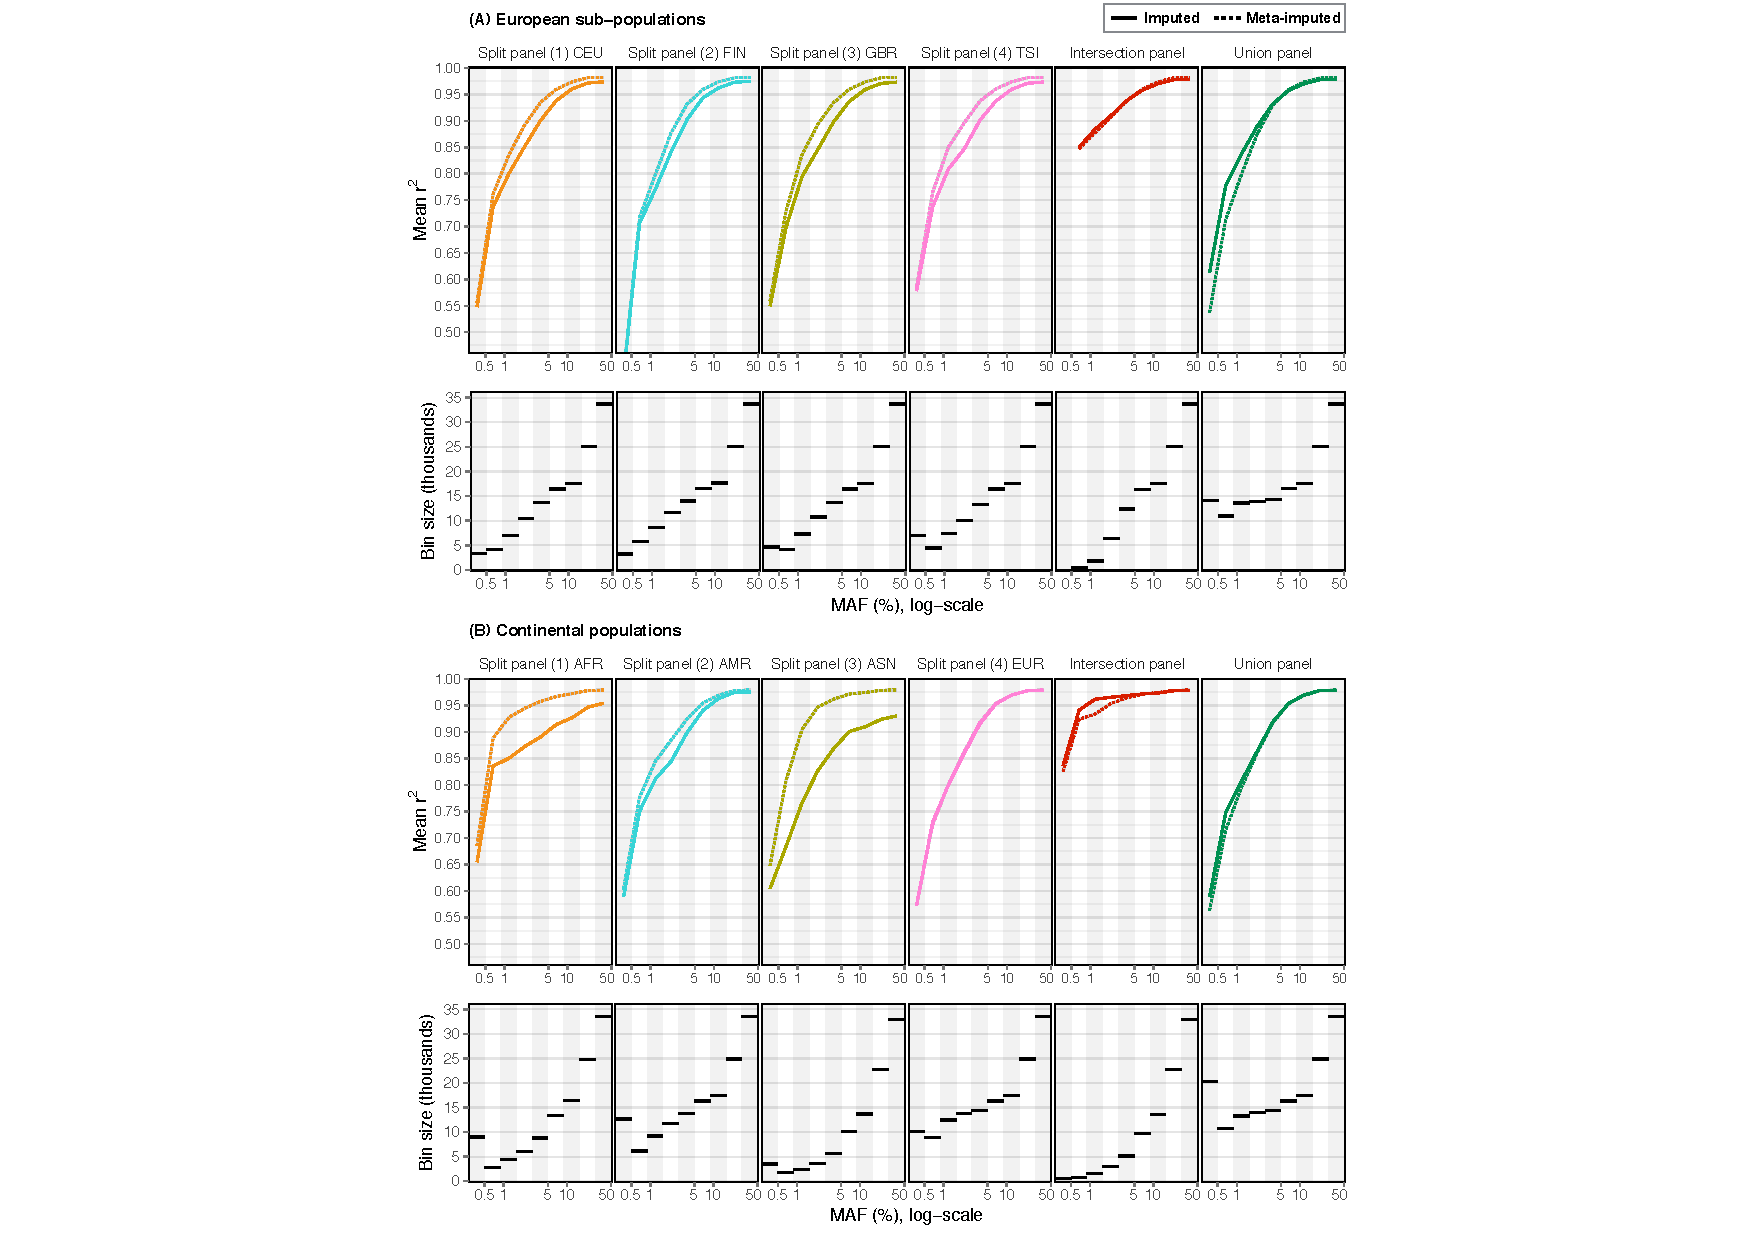
\includegraphics[width=\textwidth]{./img/ch2/accuracy_imp_maf_rsq}
\Caption{Accuracy comparison between meta-imputation and direct imputations}
{Accuracy was measured as mean~$r^2$ per \gls{maf} bin, defined on log-scale where \emph{grey-white} bars indicate boundaries.
Each imputed panel (imputations from the \n{4} split panels, the intersection panel, and the union panel) was separately compared to meta-imputation on the same set of variants per bin \Addition{(\ie on the intersected set of SNPs per comparison)}; shown for variants retained after \gls{qc}, in Scenarios~A and B.
\Gls{maf} bins were defined on the actual allele frequencies as determined by the \gls{got2d} dataset.
Note that mean~$r^2$ is not shown if the number of markers dropped below \n{50} per \gls{maf} bin.
Panels at the bottom show the number of variants compared per bin.}
{fig:imp_rsq}
\end{figure}

%

Each of the imputed datasets was compared separately to meta-imputation, on the same set of variants retained after \gls{qc}.
The distribution of accuracy (mean~$r^2$) measured by \gls{maf} is shown in \cpref{fig:imp_rsq}; average accuracy measured for each imputation strategy in comparison to meta-imputation is given in \cpref{tab:imp_rsq}, where accuracy was measured by \gls{maf} to distinguish
rare variants (${\text{MAF} \in \left[ 0.00, 0.01\right]}$),
low-frequency (${\text{MAF} \in \left( 0.01, 0.05\right]}$), and
common variants (${\text{MAF} \in \left( 0.05, 0.50\right]}$).

In Scenario~A, meta-imputation showed an improvement in accuracy over imputations from split panels.
For example, for rare variants, the highest improvement among split panel comparisons was seen with the GBR sample, where mean~$r^2$ was \MeanValue{0.6366850}{3.37107e-03} for GBR and \MeanValue{0.6589668}{3.29561e-03} for meta-imputed data.
Differences were larger at low-frequency, where the highest improvement was seen in comparison with the TSI sample;
\MeanValue{0.8647786}{1.16400e-03} and \MeanValue{0.9068669}{0.80808e-03}
for TSI and meta-imputation, respectively.
Only the union panel was higher in accuracy than meta-imputation; \eg
\MeanValue{0.6966732}{1.87252e-03} and \MeanValue{0.6266977}{2.00122e-03}
for rare variants, respectively, and
\MeanValue{0.8926102}{0.80090e-03} and \MeanValue{0.8769747}{0.85858e-03}
at low-frequency variants, respectively.
Meta-imputation showed approximately equal levels of accuracy as the union panel at common variants, where the difference in mean~$r^2$ was \MeanValue{0.003182026}{0.811088e-04}.

%
% !TEX root = ../../main.tex


\begin{table}[p]
\Caption{Accuracy of imputation strategies at rare, low-frequency, and common variants}
{Accuracy was calculated as mean~$r^2$ per \gls{maf} bin on the same set of variants retained after \gls{qc} in each comparison between meta-imputation and direct imputation, where $n$ denotes the number of variants compared.
The imputation strategy with the highest accuracy is highlighted (\textbf{bold}).
The median of KS test statistic, $\widetilde{D}_{500}$, determined whether imputed and meta-imputed \gls{maf} distributions were significantly different; see \ctref{eq:meta_ks_test}.}
{tab:imp_rsq}
\centering
\TableUnits
\begin{threeparttable}
\begin{tabular}{%
	ll%
	S[table-format=5.0]%
  S[table-format=1.3]@{}S[table-format=1.3]%
  S[table-format=1.3]@{}S[table-format=1.3]%
	S[table-format=1.3,table-align-text-post=false,table-space-text-post={*}]
	}
\toprule
{MAF bin} & {Panel} & {$n$} &
\multicolumn{2}{c}{Imputation} &
\multicolumn{2}{c}{Meta-imputation} &
{KS test$^\dagger$} \\
\cmidrule(lr){4-5}
\cmidrule(lr){6-7}
 & & & {Mean $r^2$} & {($\pm$~SE$^\ddagger$)} & {Mean $r^2$} & {($\pm$~SE$^\ddagger$)} & {$\widetilde{D}_{500}$} \\
\otoprule
\multicolumn{8}{@{ }l}{\textbf{Scenario A}\quad(European sub-populations)} \\
\midrule
{{[0.00, 0.01]}}
 & Split panel, CEU &  8636  &  0.664810 & (3.491492)  & \bfseries 0.683215 & (3.401931) & 0.046 \\
 & Split panel, FIN & 10416  &  0.619024 & (3.291918)  & \bfseries 0.629806 & (3.255431) & 0.024 \\
 & Split panel, GBR & 10023  &  0.636685 & (3.371077)  & \bfseries 0.658966 & (3.295617) & 0.034 \\
 & Split panel, TSI & 12763  &  0.653711 & (2.973932)  & \bfseries 0.670288 & (2.909213) & 0.098* \\
 \cmidrule(lr){3-8}
 & \slshape Intersection panel &   546  &  0.822921 & (9.901204)  & \bfseries 0.823535 & (9.831856) & 0.028 \\
 & \slshape        Union panel & 27712  & \bfseries 0.696673 & (1.872524)  &  0.626697 & (2.001220) & 0.264** \\
\cmidrule(lr){2-8}
{{(0.01, 0.05]}}
 & Split panel, CEU & 30012  &  0.865500 & (1.091816)  & \bfseries 0.902455 & (0.812636) & 0.040 \\
 & Split panel, FIN & 32969  &  0.853442 & (1.076218)  & \bfseries 0.885026 & (0.887284) & 0.032 \\
 & Split panel, GBR & 30442  &  0.860141 & (1.119440)  & \bfseries 0.901463 & (0.813331) & 0.036 \\
 & Split panel, TSI & 29445  &  0.864778 & (1.164005)  & \bfseries 0.906866 & (0.808084) & 0.036 \\
 \cmidrule(lr){3-8}
 & \slshape Intersection panel & 20604  & \bfseries 0.924906 & (0.849920)  &  0.923345 & (0.803135) & 0.034 \\
 & \slshape        Union panel & 39213  & \bfseries 0.892610 & (0.800904)  &  0.876974 & (0.858581) & 0.088* \\
\cmidrule(lr){2-8}
{{(0.05, 0.50]}}
 & Split panel, CEU & 92885  &  0.964461 & (0.268998)  & \bfseries 0.976659 & (0.180477) & 0.014 \\
 & Split panel, FIN & 92936  &  0.966423 & (0.249706)  & \bfseries 0.976583 & (0.181070) & 0.012 \\
 & Split panel, GBR & 92845  &  0.963589 & (0.273313)  & \bfseries 0.976622 & (0.180833) & 0.012 \\
 & Split panel, TSI & 92840  &  0.963894 & (0.283242)  & \bfseries 0.976786 & (0.179558) & 0.012 \\
 \cmidrule(lr){3-8}
 & \slshape Intersection panel & 92751  &  0.973344 & (0.211934)  & \bfseries 0.976723 & (0.180231) & 0.012 \\
 & \slshape        Union panel & 92938  &  0.973373 & (0.211659)  & \bfseries 0.976555 & (0.181358) & 0.012 \\
 \otoprule
 \multicolumn{8}{@{ }l}{\textbf{Scenario B}\quad(Continental populations)} \\
 \midrule
 {{[0.00, 0.01]}}
  & Split panel, AFR & 12495  &  0.703450 & (3.238338)  & \bfseries 0.744594 & (3.070404) & 0.030 \\
  & Split panel, AMR & 20416  &  0.653123 & (2.479939)  & \bfseries 0.672060 & (2.387583) & 0.040 \\
  & Split panel, ASN &  5661  &  0.639974 & (4.971557)  & \bfseries 0.713699 & (4.585839) & 0.082 \\
  & Split panel, EUR & 21223  & \bfseries 0.658367 & (2.226543)  &  0.656284 & (2.207200) & 0.048 \\
  \cmidrule(lr){3-8}
  & \slshape Intersection panel &  1364  & \bfseries 0.907201 & (4.420106)  &  0.891806 & (4.430467) & 0.172** \\
  & \slshape        Union panel & 33430  & \bfseries 0.653383 & (1.871343)  &  0.626010 & (1.894104) & 0.148** \\
 \cmidrule(lr){2-8}
 {{(0.01, 0.05]}}
  & Split panel, AFR & 18468  &  0.879161 & (1.631274)  & \bfseries 0.948322 & (0.766896) & 0.048 \\
  & Split panel, AMR & 33093  &  0.860770 & (1.157715)  & \bfseries 0.893814 & (0.855185) & 0.036 \\
  & Split panel, ASN & 11181  &  0.836930 & (2.413587)  & \bfseries 0.947709 & (0.953756) & 0.114** \\
  & Split panel, EUR & 38417  & \bfseries 0.867048 & (0.968714)  &  0.869536 & (0.909904) & 0.032 \\
  \cmidrule(lr){3-8}
  & \slshape Intersection panel &  9443  & \bfseries 0.967004 & (0.810571)  &  0.956752 & (0.815682) & 0.062 \\
  & \slshape        Union panel & 39140  & \bfseries 0.870742 & (0.948816)  &  0.866276 & (0.923712) & 0.058 \\
 \cmidrule(lr){2-8}
 {{(0.05, 0.50]}}
  & Split panel, AFR & 88152  &  0.941104 & (0.425965)  & \bfseries 0.976002 & (0.172260) & 0.022 \\
  & Split panel, AMR & 92144  &  0.966958 & (0.263392)  & \bfseries 0.972889 & (0.191426) & 0.016 \\
  & Split panel, ASN & 79581  &  0.921305 & (0.518841)  & \bfseries 0.977514 & (0.165172) & 0.024 \\
  & Split panel, EUR & 92188  &  0.972060 & (0.217795)  & \bfseries 0.972762 & (0.192505) & 0.016 \\
  \cmidrule(lr){3-8}
  & \slshape Intersection panel & 79051  &  0.976452 & (0.201266)  & \bfseries 0.977380 & (0.167886) & 0.016 \\
  & \slshape        Union panel & 92187  & \bfseries 0.972790 & (0.213868)  &  0.972755 & (0.192606) & 0.016 \\
\bottomrule
\end{tabular}
\begin{tablenotes}\footnotesize
	\item[{${\dagger}$}] Median of the Kolmogorov–Smirnov (KS) test statistic, $\widetilde{D}$; empirical CDF of imputed and meta-imputed \gls{maf} tested at ${\alpha = 0.05}$ ($\ast$) and ${\alpha = 0.01}$ (${\ast\ast}$).
	\item[{${\ddagger}$}] Standard error (SE) $\times 10^{-3}$.
\end{tablenotes}
\end{threeparttable}
\end{table}

%

Genotype accuracy showed higher differences in Scenario~B, where meta-imputation improved accuracy in most split panel comparisons.
For rare variants, the highest difference was seen to genotype data imputed from the AFR split panel, where mean~$r^2$ was \MeanValue{0.7034507}{3.23833e-03}, compared to \MeanValue{0.7445944}{3.07040e-03} for meta-imputed genotypes.
However, meta-imputation showed similar accuracy as the imputation from the EUR sample, where the difference in mean~$r^2$ was \MeanValue{0.002083192}{0.715902e-04}.
Likewise, at low-frequency, mean~$r^2$ was \MeanValue{0.879161}{1.63127e-03} for AFR and \MeanValue{0.948322}{0.76689e-03} for meta-imputation, and the difference in accuracy was \MeanValue{0.002487}{0.36658e-03} with regard to the EUR split panel.
As in Scenario~A, differences were smaller for common variants, such that the difference in mean~$r^2$ was below \dec{0.001} in comparisons to imputations from the AFR, AMR, and EUR panels, but where the ASN sample showed the highest difference; mean~$r^2$ was \MeanValue{0.921305}{0.51884e-03} for ASN and \MeanValue{0.977514}{0.16517e-03} for meta-imputation.
The union panel was similar in accuracy as meta-imputation, where the overall difference in mean~$r^2$ was \MeanValue{0.01062464}{8.471535e-03}.

Imputations from the intersection panel in Scenario~A and B showed approximately equal levels of accuracy to meta-imputation.
The difference in mean~$r^2$ averaged to \MeanValue{0.0008106733}{1.429231e-04} across \gls{maf} in Scenario~A, and \MeanValue{0.008239279}{4.8183e-03} in Scenario~B.
However, note that the number of variants in the intersection panel was the lowest among available panel data in both scenarios (\cref{tab:imp_qc}), and was further reduced as accuracy was measured on the same sets of variants retained in both the intersection and the meta-imputed datasets.
For example, the comparison between the intersection panel and meta-imputation included only \n{546} variants at \gls{maf} ${\leq 1\%}$ in Scenario~A and \n{1364} variants in Scenario~B, whereas each split panel and the union panel were compared on several thousands of variants at this frequency range.
The high accuracy of genotypes imputed from the intersection panel may result from retaining only those variants that are ``cosmopolitan'' within the scope of the present evaluation.


%
%!TEX root = ../../main.tex


\begin{figure}[!htb]
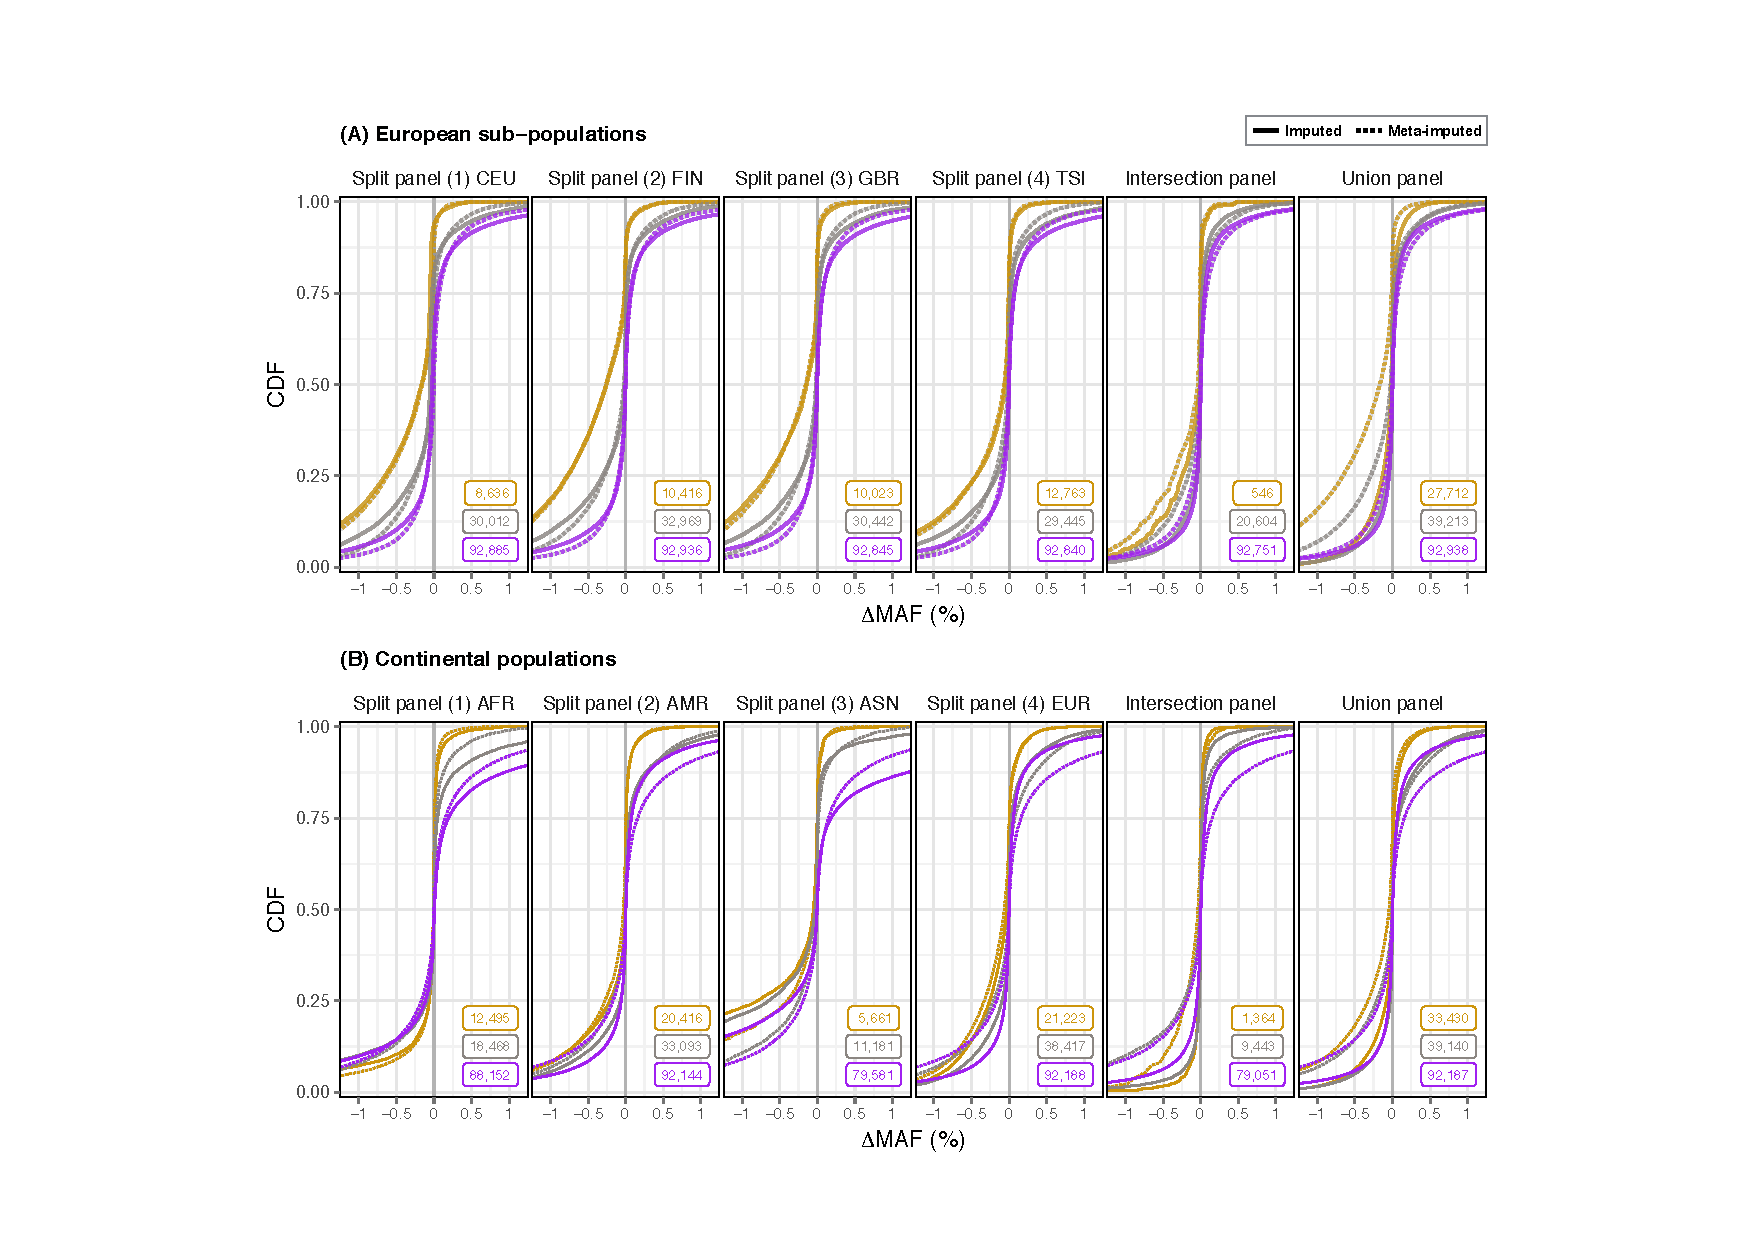
\includegraphics[width=\textwidth]{./img/ch2/accuracy_imputed_delta}
\Caption{Difference between imputed and masked minor allele frequency}
{Comparison of imputed and meta-imputed \gls{maf} in relation to known population frequencies, compared on the same set as retained after \gls{qc} in each comparison.
Frequency difference, ${\Delta\text{MAF}}$, was calculated as the \gls{maf} observed at a masked variant minus \gls{maf} at the corresponding (meta-)imputed variant, pooled in \n{3} \gls{maf} bins; rare variants (${\text{MAF} \in \left[ 0.00, 0.01\right]}$; \emph{yellow}), low-frequency (${\text{MAF} \in \left( 0.01, 0.05\right]}$; \emph{grey}), and common variants (${\text{MAF} \in \left( 0.05, 0.50\right]}$; \emph{purple}).
Numbers per \gls{maf} bin per comparison are given in each panel (\emph{colour-coded}).}
{fig:imp_delta}
\end{figure}

%

Further, the empirical \gls{cdf} of \gls{maf} at imputed and meta-imputed variants was compared per \gls{maf} bin.
Differences are illustrated in \cpref{fig:imp_delta}, which shows the \gls{cdf} of compared variants in relation to the known population frequencies at masked variants in the \gls{got2d} dataset; calculated by subtracting (meta-)imputed frequencies from masked frequencies (${\Delta\text{MAF}}$) at the same set of markers.
Notably, meta-imputed frequencies showed high consistency with imputed frequencies at rare variants (${\text{MAF} \in \left[ 0.00, 0.01\right]}$) across split panel imputations, but were skewed in comparison to imputations from the union panel in both scenarios.
Significant differences were found for rare variant imputations from the TSI sample (${\widetilde{D}=0.098}$) in Scenario~A, as well as for the union panel at rare and low-frequency variants (\dec{0.264} and \dec{0.088}, respectively).
In Scenario~B, imputed and meta-imputed differences were significantly different for rare variant imputations from the intersection panel and the union panel (\dec{0.172} and \dec{0.148}, respectively) and for the union panel at low-frequency variants (\dec{0.114}).
These results suggested that meta-imputation was able to correctly reproduce realistic allele frequency distributions from the combination of imputed genotypes from different sources, while achieving higher or similar accuracy compared to direct imputations from split panels.
Results of KS tests in each comparison are given in \cpref{tab:imp_rsq}.


In summary, split panel imputations were either outperformed or similar levels of accuracy were achieved in direct comparisons to meta-imputed data; see \cref{tab:imp_rsq} for a complete summary of genotype accuracy measured in each comparison.
Although imputations from the union panel outperformed meta-imputation, such differences may be expected given that the union panel contained all the information which meta-imputation had to leverage indirectly from several data sources.
Nonetheless, the present evaluation of genotype accuracy was limited with regard to coverage; for instance, genotype data imputed from the intersection panel was found to be relatively high in accuracy and similar with regard to meta-imputed data, but the low number of variants present in the intersection panel may not yield similar improvements under realistic conditions in association analyses.
Therefore, to provide a comprehensive assessment of the meta-imputation method and to account for a potential tradeoff between accuracy and coverage, I conducted a more extensive power analysis in the following section.



%
\section{Power to detect significant risk signals}
\label{sec:metaimpute_power}
%

The power of meta-imputation to detect disease risk factors in association tests was evaluated using simulated sample data.
This was done in consideration of expected power when causal risk factors vary in their allele frequency as well as risk effect size.
In particular, a series of simulated case-control association experiments was conducted, from which the power to detect significant association signals was determined, at specified allele frequencies and effect size of simulated risk factors.
The description of the methods used is provided below (\ccref{sec:meta_power_methods}), followed by the presentation of results (\ccref{sec:meta_power_results}).


%
\subsection{Methods}
\label{sec:meta_power_methods}
%

The same regime to carry out imputation and \gls{qc} was followed as described in \cpref{sec:meta_accuracy_methods}.
An additional set of haplotype reference data was available from \n{4} independent sequencing studies, which were included here as Scenario~C; see below.
\begin{description}
	\item[Finns.] A Finnish cohort composed of data from the Sequencing Initiative Suomi Project (\emph{SISu}) and the \emph{Finrisk} Project \citep{Vartiainen:2010eb,Pajunen:2010ft,Lim:2014ir,Borodulin:2015bs}; 4x depth; sample size and number of \glspl{snp} considered here were ${N=\num{1941}}$ and ${M=\num{283654}}$, respectively.
	\item[GoNL.] The Genome of the Netherlands Project \citep{Boomsma:2013hf, Deelen:2014dq, GenomeoftheNetherlandsConsortium:2014gs}; 12x depth, consisting of a representative sample of \n{250} trio-families; ${N=\num{748}}$, ${M=\num{362694}}$.
	\item[ORCADES.] The Orkney Complex Disease Study of genetic epidemiology of an isolated population in northern Scotland \citep{McQuillan:2008fz}; 4x depth, family-based data; ${N=\num{399}}$, ${M=\num{236755}}$.
	\item[UK10K.] The \emph{UK10K} Genome Sequencing Project \citep{UKKConsortium:2015ii}; 6.5x depth; ${N=\num{3642}}$, ${M=\num{527199}}$.
\end{description}
Also, an intersection panel was prepared from these \n{4} datasets, but no union panel.
As before, only data from chromosome~20 were considered.
Note that the above datasets were part of the early stage \gls{hrc} testing phase \citep{McCarthy:2016gs}.\footnote{Acknowledgement: Data provided by Professor Jonathan Marchini, Department of Statistics, University of Oxford; prior to the release of the \gls{hrc} dataset.}


%
\subsubsection{Simulation of study sample data}
%

Simulations were performed using \texttt{HAPGEN} version~2.2.0 \citep{Su:2011km}, which requires a \emph{template} dataset of haplotypes to reproduce realistic variant data in \gls{hwe}, such that \gls{ld} patterns in the simulated dataset are consistent with the haplotype sample.
Individual sites can be simulated to independently act as causal disease variants with specified relative risk.
The simulation generates \n{2} \gls{gwa} samples of individuals that are affected (\emph{cases}) or not affected (\emph{controls}) by a disease phenotype.
Data are identical in coverage as the template dataset.

Here, simulations were performed using \gls{got2d} data (chromosome~20) to serve as the template dataset.
The size of simulated case and control samples was fixed to \n{2500} individuals each.
Although a larger sample would have been beneficial in terms of signal detection through association testing, exceeding the size of the template dataset (${N=\num{2657}}$) was expected to result in factitious allele frequency changes.
For example, an iterative re-sampling strategy could be applied to introduce new low-frequency variants \citep[\eg following][]{Moutsianas:2015jm}.
However, this was not done here because the effect size of risk variants (as defined during simulation) would likely be affected by such a sampling process.

A series of simulation experiments was conducted in which \n{1} variant was selected per simulation to act as a causal risk factor.
Its relative risk (RR) was defined for heterozygous genotypes ($RR_{het}$) in a log-additive disease model (\ie multiplicative on linear scale); the following \n{3} risk categories were defined.
\begin{align*}
	\textit{Low risk}     : & \quad {RR_{het}=1.2} \quad {(RR_{hom}=1.44)} \\
	\textit{Modest risk}  : & \quad {RR_{het}=1.6} \quad {(RR_{hom}=2.56)} \\
	\textit{High risk}    : & \quad {RR_{het}=2.0} \quad {(RR_{hom}=4.00)}
\end{align*}
The analysis was performed by conducting \n{300} replicate simulations per risk category, where variants occurring at different frequencies were selected in \n{3} defined \gls{maf} intervals;
very low frequency (${\text{MAF} \in [0.5, 1]\,\%}$), low frequency (${\text{MAF} \in (1, 5]\,\%}$), and high frequency (${\text{MAF} \in (5, 50]\,\%}$), such that \n{100} variants were drawn from each interval and simulated as risk variants.

Note that variant selection was done at random, regardless of presence or absence of the selected variant in any of the available reference panels, so as to mirror conditions encountered under realistic \gls{gwa} settings; \ie when a causal variant itself is absent in an imputation reference, its risk effects may be detectable through \gls{ld} at neighbouring sites.

%
% !TEX root = ../../main.tex


\begin{figure}[!htb]
\centering
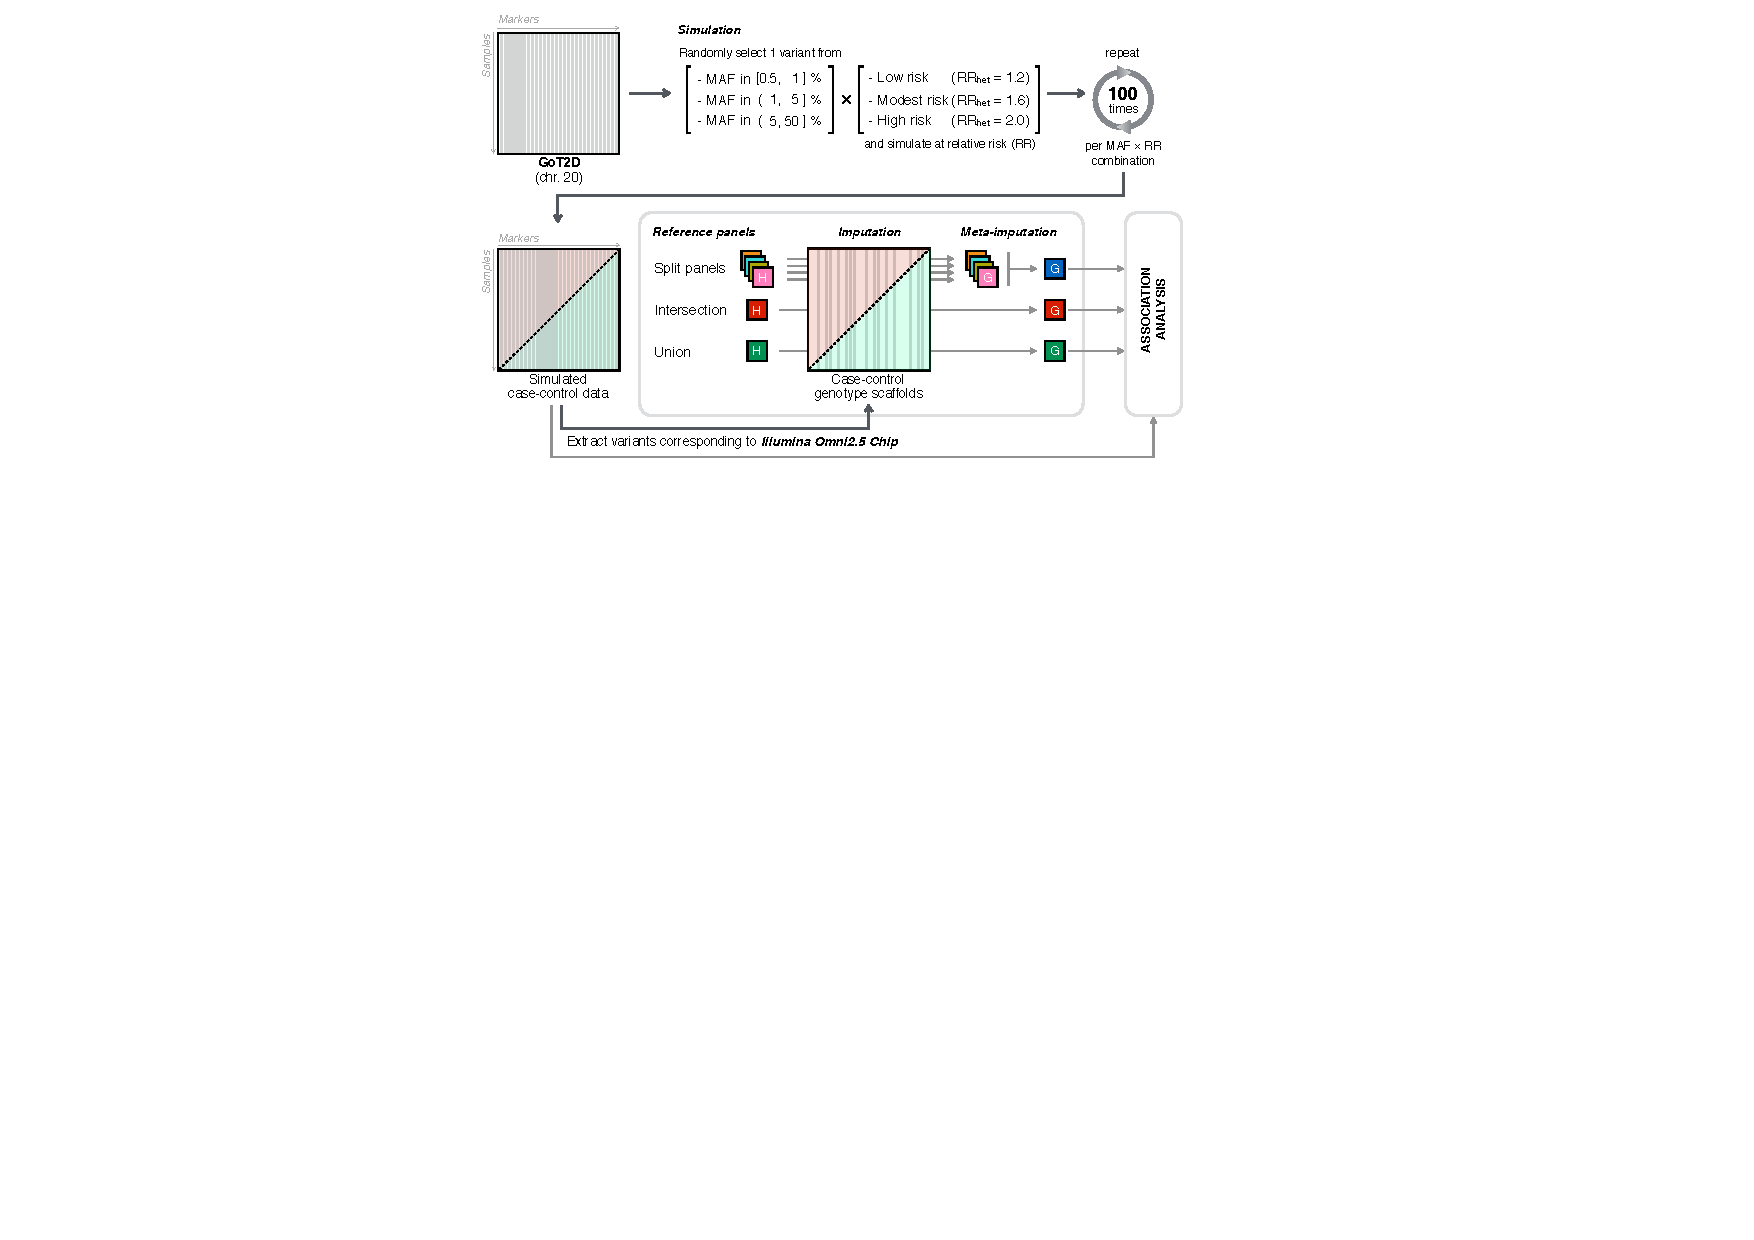
\includegraphics[width=0.9\textwidth]{./img/ch2/info_design_power}
\Caption{Illustration of the simulation process}
{Meta-imputation was assessed in terms of statistical power to detect significant risk association signals in a series of simulated case-control experiments.
The \gls{got2d} dataset was used as a template for simulations using \texttt{HAPGEN} \citep{Su:2011km}, where \n{1} variant was randomly selected within \n{1} of \n{3} defined \gls{maf} intervals.
The selected variant was then simulated to act as a causal disease variant in the simulated case-control dataset, where relative risk ($RR_{het}$) was defined according to \n{1} of \n{3} defined risk categories.
In total, \n{100} replicate simulations were conducted per combination of \gls{maf} interval and risk category (per scenario).
Simulated data were used to extract a genotype scaffold into which available reference panels were imputed, followed by meta-imputation of imputed datasets.
Imputed and meta-imputed datasets were then subjected to association analysis, including the simulated (not imputed) datasets for comparison.}
{fig:info_design_power}
\end{figure}

%

To generate a study sample for imputations, a variant scaffold was extracted from each simulation replicate.
Because the set of simulated variants mirrored those in the \gls{got2d} dataset,
sites that matched with variants typed on \emph{Illumina Omni2.5 Array} were identified and extracted.
A scaffold thus contained \n{40255} variants into which available reference panels were imputed.
Note that simulations produced \n{2} datasets; \n{1} case and \n{1} corresponding control dataset.
These were concatenated before imputation to ensure consistency in the imputation analysis.
Imputed data were again separated into case and control samples prior to association analysis (described below).
Because \texttt{HAPGEN2} produces haplotype data, imputations were executed on pre-phased genotypes.
A summary of the simulation process is illustrated in \cpref{fig:info_design_power}.



%
\subsubsection{Association analysis in imputed genotype data}
%

Imputed case and control datasets were analysed using a frequentist score test under an additive model of association, implemented in \texttt{SNPTEST} version~2.5 \citep{Marchini:2007bg}.
In contrast to the previous analysis (\ctref{metaimpute_accuracy}), in which the variants not included in the extracted scaffold were masked to measure accuracy after imputation, here, the simulated case-control dataset was retained and separately examined in association analysis.
This was done to enable comparisons of meta-imputed and imputed data to a non-imputed benchmark result for each simulation replicate.

The genomic control inflation factor, $\lambda_\text{GC}$, was calculated to investigate if systematic biases are present in association results, which is defined as the median of $\chi^2$~test statistics resulting from case-control association tests divided by the expected median of the $\chi^2$~distribution \citep{Devlin:2001ga}.
Because the frequentist score test was used, $\lambda_\text{GC}$ was calculated on basis of the resulting \pvalues from which the $\chi^2$~statistic was calculated with \n{1} degree of freedom.


%
\subsubsection{Calculation of power in replicate simulation experiments}
%

Significant association signals were identified in each simulation and pooled by \gls{maf} interval and risk category, according to which variants were selected and simulated.
The proportion of datasets in which significance was reached at the known risk variant was taken as a simple estimate for the statistical power to detect genetic risk effects.
Note that the position of the simulated risk variant was known through simulation, but the variant itself may not be retained after imputation or \gls{qc}.
Therefore, signal detection was performed within a 1~\gls{Mb} region around the position of the simulated risk variant, for any site reaching significance with this region.

Significance was defined at a nominal threshold of ${\pvalue\leq1\times10^{-6}}$.
Note that this threshold is higher (thus, less conservative) than commonly applied genome-wide thresholds, \eg at \num{5e-8} \citep[\eg, see][]{Risch:1996ub}, because analyses were conducted on data from chromosome 20 only.
However, to provide additional detail, power was estimated under a moving significance threshold; between ${\pvalue\leq1\times10^{-8}}$ and ${\pvalue\leq1\times10^{-4}}$.
As a comparative measure between association results produced from the different imputation strategies,
the difference in power between the non-imputed simulation dataset and a given (meta-)imputed dataset is reported, denoted by ${\Delta_P}$, which is calculated as the average difference along the moving significance threshold.


%
\subsection{Results}
\label{sec:meta_power_results}
%

A number of \n{100} variants were selected per \gls{maf} interval such that there were 300 variants in total.
Each was then simulated at the \n{3} defined risk categories such that \n{900} simulations were conducted
from which a genotype scaffold was extracted for imputation.
Given the \n{4} split panels, the intersection panel, and the union panel available per Scenario~A and B, as well as the \n{4} independent reference datasets and the generated intersection panel in Scenario~C, a total of \n{15300} imputation analyses were performed.
Imputed data were then combined in meta-imputation (except the intersection and union panels), resulting in \n{900} additional genotype datasets.
Each dataset was then subjected to association analysis, including the non-imputed simulated case-control sample, which was used as a benchmark for comparisons.
Hence, a total of \n{17100} association analyses were conducted, where each was treated as an independent \gls{gwa} study.
All analyses were performed on whole-chromosome data (chromosome~20).


%
%!TEX root = ../../main.tex


\begin{figure}[!htb]
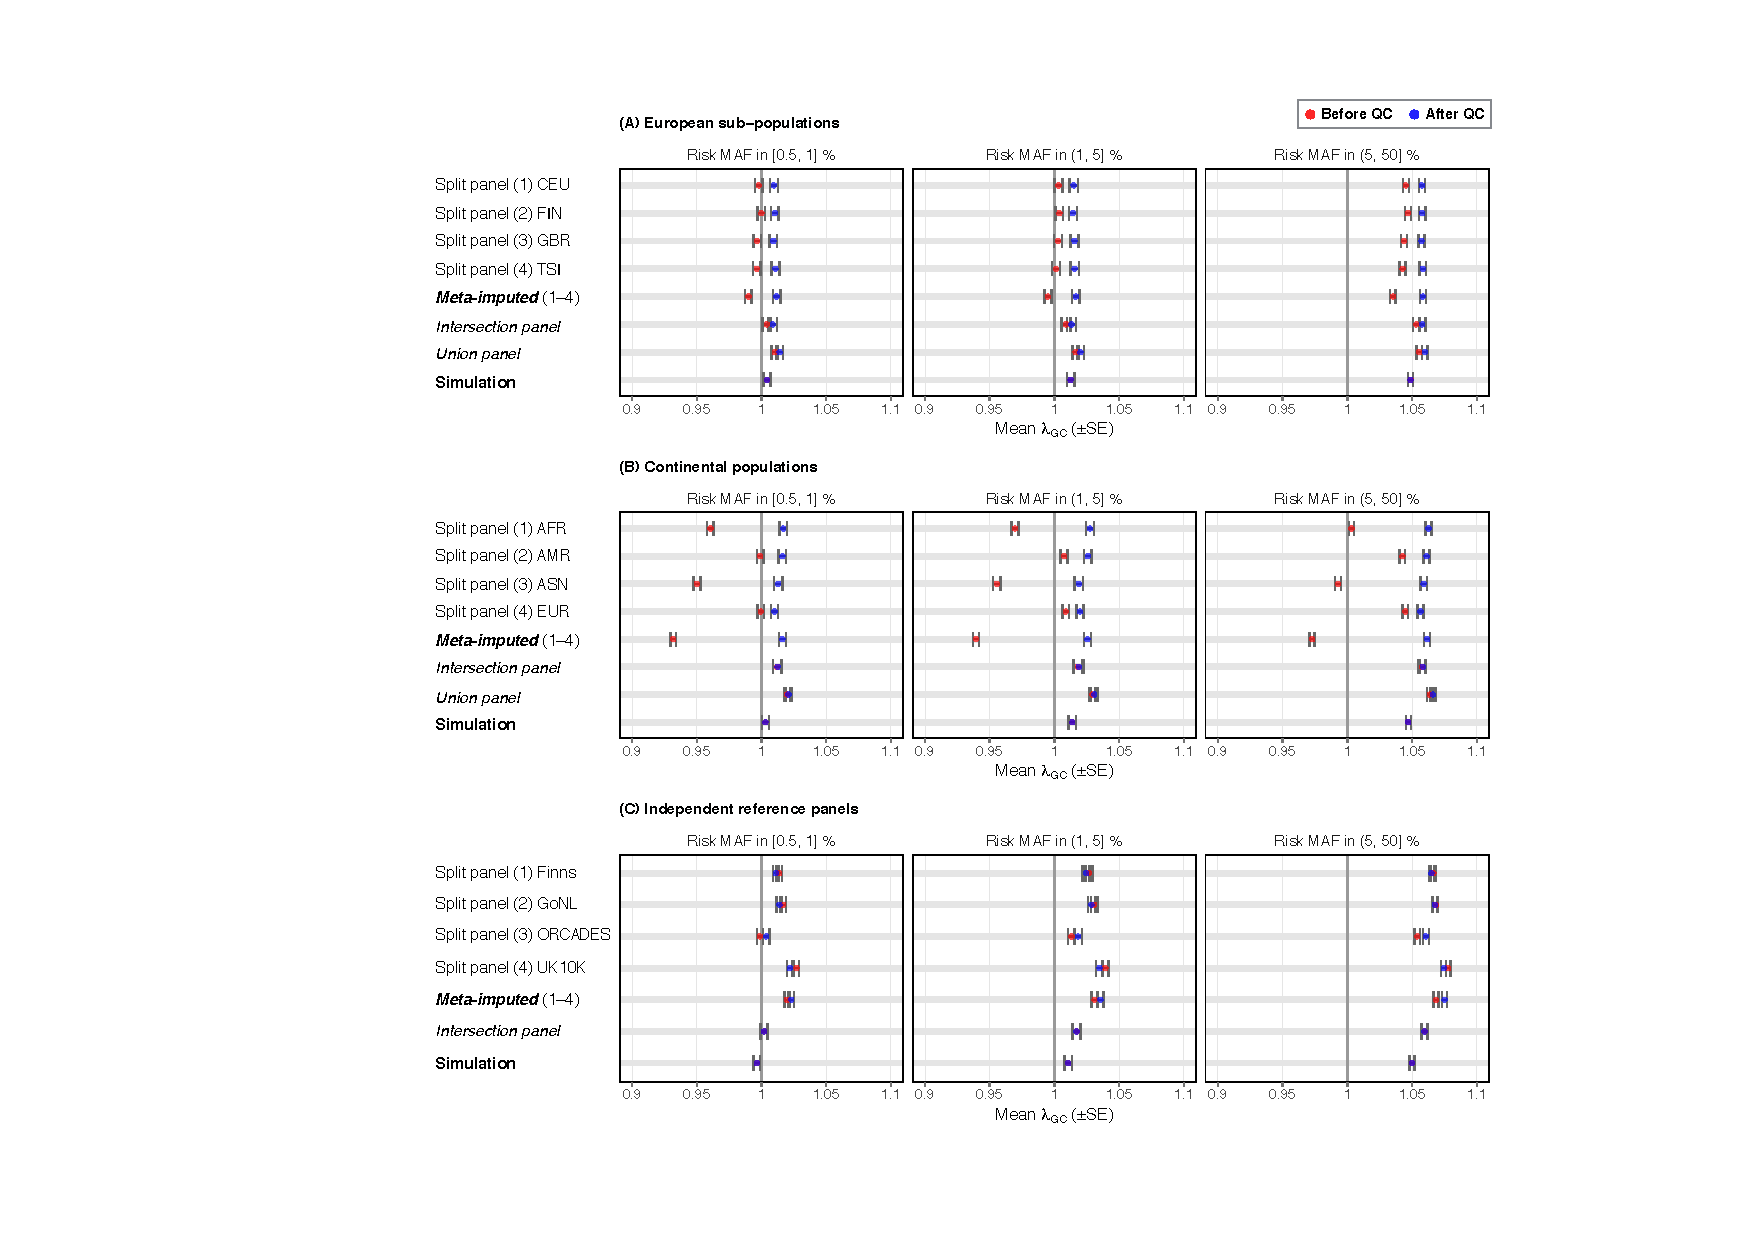
\includegraphics[width=\textwidth]{./img/ch2/association_lambda}
\Caption{Inflation observed in simulated case-control experiments}
{Genomic control inflation factor calculated before (\emph{red}) and after (\emph{blue}) variants were filtered in \gls{qc}, reported as mean $\lambda_\text{GC}$ over replicate association results by \gls{maf} of the simulated risk variants.}
{fig:power_lgc}
\end{figure}

%

Association results were inspected with regard to inflation before and after \gls{qc}; the difference is shown in \cpref{fig:power_lgc} where $\lambda_\text{GC}$ is shown as the average per \gls{maf} interval.
Inflation was slightly increased at higher \Addition{risk variant} frequencies.
The difference of $\lambda_\text{GC}$ before and after \gls{qc} was small in Scenarios A~and~C, but noticeable in Scenario~B, where association results of meta-imputed data were deflated (${\lambda_\text{GC} < 1}$) before \gls{qc}.
After \gls{qc}, $\lambda_\text{GC}$ values of all imputed and meta-imputed datasets were approximately equal to inflation measured for the non-imputed simulation dataset in each scenario.

\Addition{Association results were at ${\lambda_\text{GC} \approx 1}$ on average in each scenario when the simulated risk variant was very low in frequency (${\text{MAF} \in [0.5, 1]\,\%}$), but increased to ${\lambda_\text{GC} \approx 1.05}$ for risk variants at higher frequencies (${\text{MAF} \in [5, 50]\,\%}$).
Although these results suggested no major inflation, higher values of $\lambda_\text{GC}$ are generally expected in presence of population sub-structure, including cryptic relationships among individuals in the sample.
One explanation why $\lambda_\text{GC}$ increased at higher risk variant frequencies is that individuals in the case sample appeared to be more related to each other than the individuals in the control sample.}

%
%!TEX root = ../../main.tex


\begin{figure}[tb]
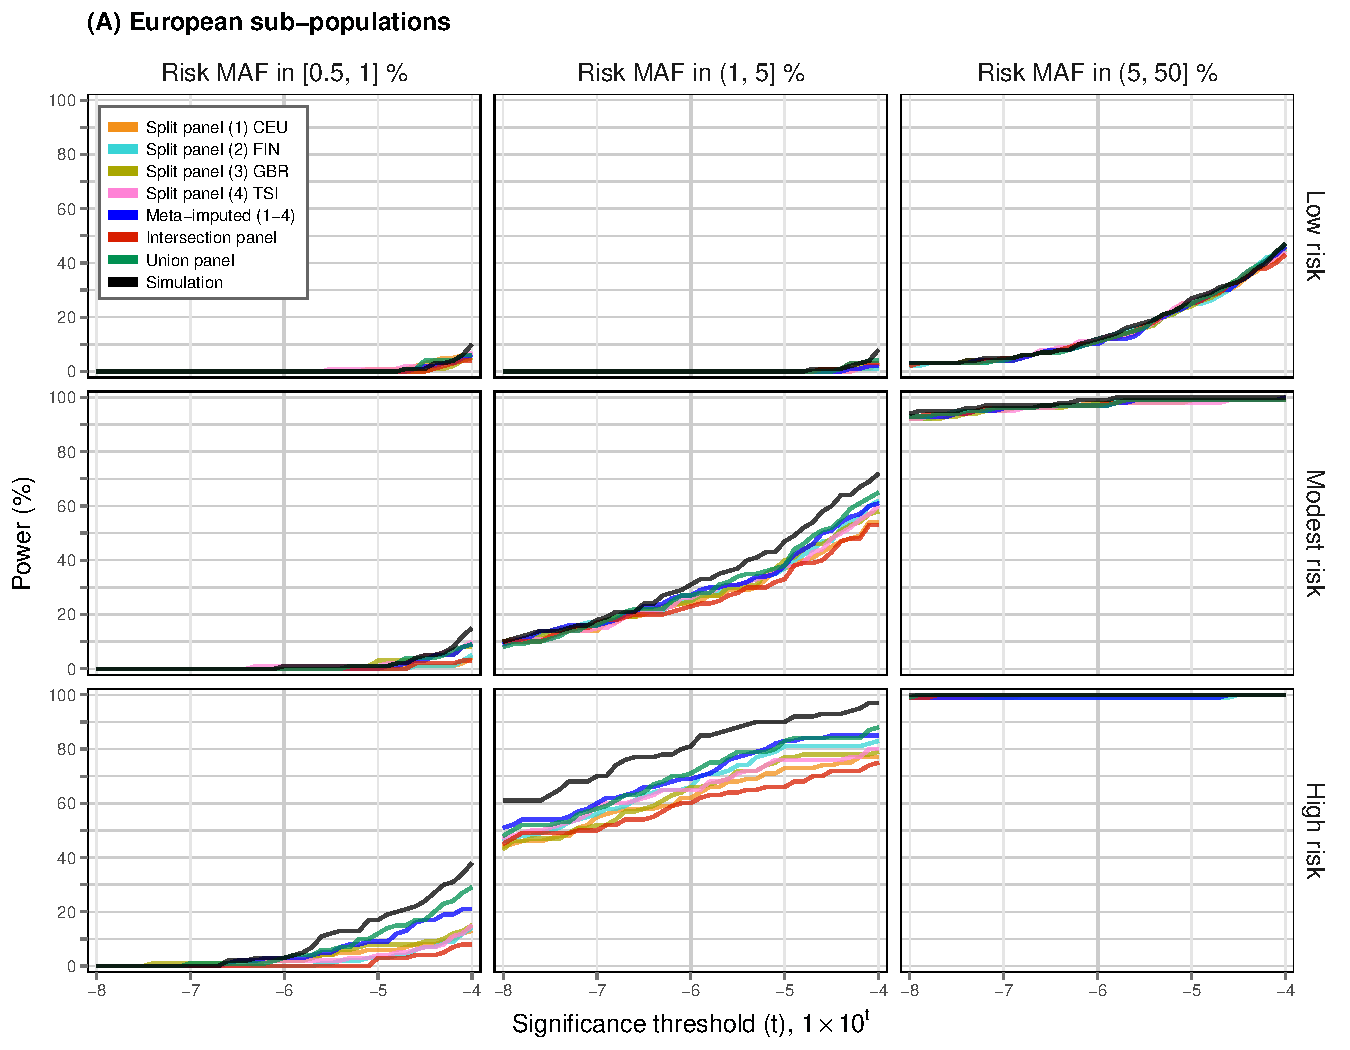
\includegraphics[width=\textwidth]{./img/ch2/plot_association_power_A}
\Caption{Power measured under a moving significance threshold}
{Power was calculated as the proportion of replicate association analyses ($n=100$, per combination of risk category and \gls{maf} interval) in which any signal reached significance within 1~\gls{Mb} around the position of a simulated risk variant.
A moving significance threshold between ${\pvalue\leq\num{1e-8}}$ and ${\pvalue\leq\num{1e-4}}$ was applied to each association dataset.\CorrectLabel}
{fig:gwas_power_A}
\end{figure}



\begin{figure}[tb]
\ContinuedFloat
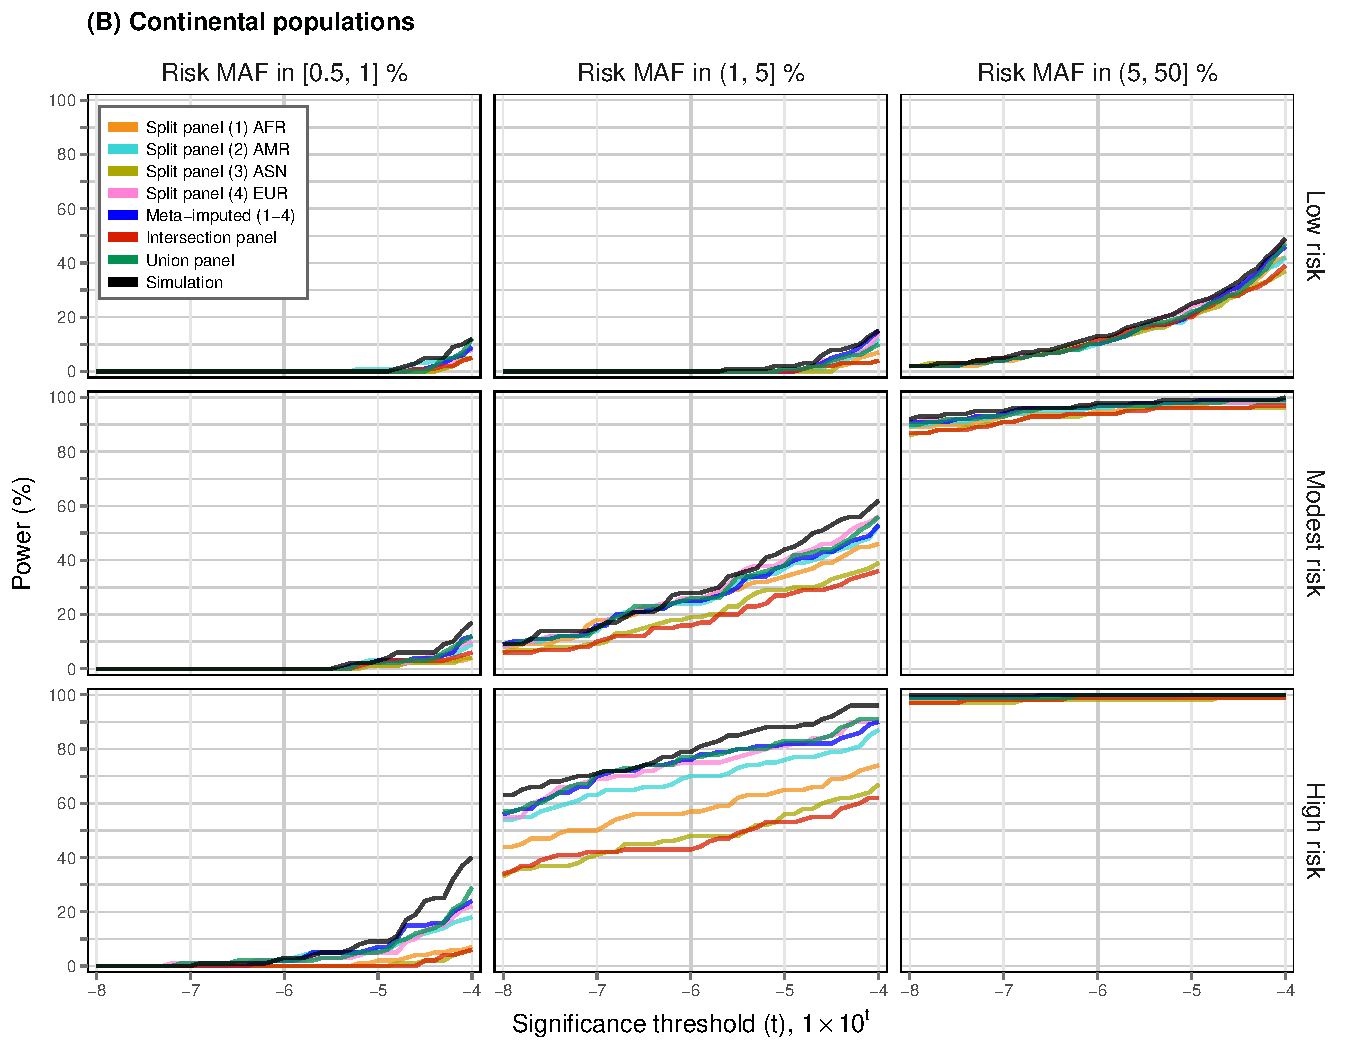
\includegraphics[width=\textwidth]{./img/ch2/plot_association_power_B}
\caption[]{Continued.\CorrectLabel}
\label{fig:gwas_power_B}
\end{figure}



\begin{figure}[tb]
\ContinuedFloat
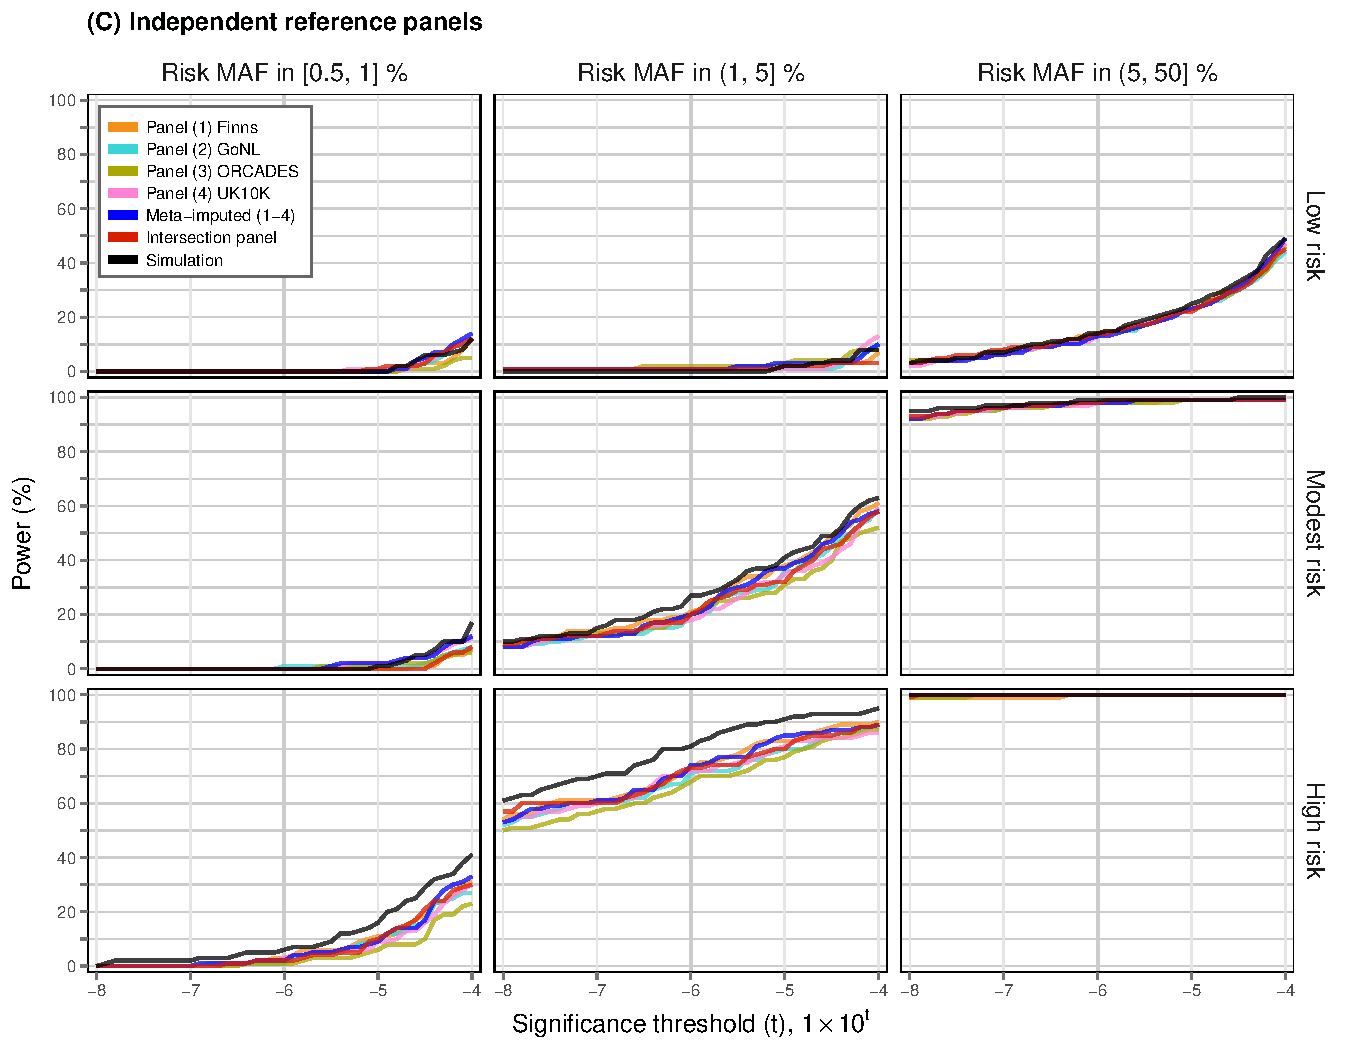
\includegraphics[width=\textwidth]{./img/ch2/plot_association_power_C}
\caption[]{Continued.\CorrectLabel}
\label{fig:gwas_power_C}
\end{figure}

%

%
% !TEX root = ../../main.tex


\begin{table}[!htb]
\Caption{Estimated power per imputation strategy}
{Power was estimated as the proportion of significant association signals found among replicate simulation experiments, for which \n{1} variant per simulation was selected at random from \n{3} \gls{maf} intervals (as specified in the table).
Each of the selected variants was simulated to act as a causal risk factor, where relative risk was simulated in \n{3} categories; low (${RR_{het}=1.2}$), modest (${RR_{het}=1.6}$), and high risk (${RR_{het}=2.0}$).
Power at a nominal significance threshold (${\pvalue\leq1\times10^{-6}}$) is reported at each combination of \gls{maf} interval and risk category.
The average difference ($\Delta_P$) in relation to the non-imputed simulation benchmark is given per \gls{maf} interval for each imputation strategy; the lowest average difference is highlighted (\textbf{bold}).
This table shows the results obtained for imputed and meta-imputed data in Scenario~A; results for Scenario~B (\pref{tab:stats_power_B}) and Scenario~C (\pref{tab:stats_power_C}) are shown separately.}
{tab:stats_power_A}
\centering
\TableUnits
\begin{threeparttable}
\begin{tabular}{%
 ll%
 S[table-format=5.0]%
 S[table-format=5.0]%
 S[table-format=5.0]%
 S[table-format=2.3]@{}S[table-format=1.3]%
 }
\multicolumn{7}{@{}l}{\bfseries (A) European sub-populations} \\
\toprule
 {Risk MAF (\%)} & {Panel} &
 \multicolumn{3}{c}{Power (\%), $\text{\pvalue} \leq 1\times10^{-6}$} &
 \multicolumn{2}{c}{$\Delta_P$ (\%)$^\ast$} \\
 \cmidrule(lr){3-5}
 \cmidrule(lr){6-7}
 & & {Low} & {Modest} & {High} & {Mean} & {($\pm$~SE)} \\
\otoprule
$[0.5, 1]$
 &  Split panel (1) CEU         &   0 &   0 &   2 &  2.53658  &  (0.48656) \\
 &  Split panel (2) FIN         &   0 &   0 &   0 &  3.04065  &  (0.51969) \\
 &  Split panel (3) GBR         &   0 &   0 &   2 &  2.09756  &  (0.44389) \\
 &  Split panel (4) TSI         &   0 &   1 &   2 &  2.30894  &  (0.50863) \\
\cmidrule(lr){3-7}
 &  Meta-imputed (1-4)          &   0 &   0 &   3 &  1.55284  &  (0.28912) \\
 & \slshape  Intersection panel &   0 &   0 &   0 &  3.36585  &  (0.59253) \\
 & \slshape  Union panel        &   0 &   0 &   3 & \bfseries 1.04878  &  (0.20614) \\
\cmidrule(lr){2-7}
$(1, 5]$
 &  Split panel (1) CEU         &   0 &  24 &  62 &  8.56097  &  (0.72925) \\
 &  Split panel (2) FIN         &   0 &  25 &  66 &  6.37398  &  (0.54277) \\
 &  Split panel (3) GBR         &   0 &  25 &  66 &  7.43089  &  (0.67039) \\
 &  Split panel (4) TSI         &   0 &  26 &  65 &  7.12195  &  (0.60514) \\
\cmidrule(lr){3-7}
 &  Meta-imputed (1-4)          &   0 &  27 &  69 &  4.95934  &  (0.43109) \\
 & \slshape  Intersection panel &   0 &  23 &  60 &  9.56097  &  (0.84577) \\
 & \slshape  Union panel        &   0 &  27 &  71 & \bfseries 4.84552  &  (0.41641) \\
\cmidrule(lr){2-7}
$(5, 50]$
 &  Split panel (1) CEU         &  11 &  98 & 100 &  0.78048  &  (0.06784) \\
 &  Split panel (2) FIN         &  12 &  98 &  99 &  0.89430  &  (0.07004) \\
 &  Split panel (3) GBR         &  11 &  98 & 100 &  0.82113  &  (0.08327) \\
 &  Split panel (4) TSI         &  11 &  97 & 100 &  0.74796  &  (0.08986) \\
\cmidrule(lr){3-7}
 &  Meta-imputed (1-4)          &  10 &  97 &  99 &  0.95934  &  (0.06868) \\
 & \slshape  Intersection panel &  11 &  97 & 100 &  0.63414  &  (0.07325) \\
 & \slshape  Union panel        &  11 &  97 & 100 & \bfseries 0.53658  &  (0.06760) \\
 \bottomrule
\end{tabular}
\begin{tablenotes}\footnotesize\DefaultUnits
 \item[{${\ast}$}] Average difference in power between simulated and (meta-)imputed association results ($\Delta_P$);
 averaged over risk category (low, modest, and high risk) and association signals detected at a moving significance threshold; between ${\pvalue\leq\num{1e-08}}$ and ${\pvalue\leq\num{1e-04}}$.
\end{tablenotes}
\end{threeparttable}
\end{table}



\begin{table}[!htb]
\ContinuedFloat
\small
\caption[]{Continued.}
\label{tab:stats_power_B}
\centering
\TableUnits
\begin{threeparttable}
\begin{tabular}{%
	ll%
	S[table-format=5.0]%
	S[table-format=5.0]%
	S[table-format=5.0]%
	S[table-format=2.3]@{}S[table-format=1.3]%
	}
 \multicolumn{7}{@{}l}{\bfseries (B) Continental populations} \\
\toprule
 {Risk MAF (\%)} & {Panel} &
 \multicolumn{3}{c}{Power (\%), $\text{\pvalue} \leq 1\times10^{-6}$} &
 \multicolumn{2}{c}{$\Delta_P$ (\%)$^\ast$} \\
 \cmidrule(lr){3-5}
 \cmidrule(lr){6-7}
 & & {Low} & {Modest} & {High} & {Mean} & {($\pm$~SE)} \\
\otoprule
$[0.5, 1]$
 &  Split panel (1) AFR        &   0 &   0 &   0 &  3.00000  &  (0.54124)  \\
 &  Split panel (2) AMR        &   0 &   0 &   3 &  1.48780  &  (0.33724)  \\
 &  Split panel (3) ASN        &   0 &   0 &   0 &  3.20325  &  (0.58263)  \\
 &  Split panel (4) EUR        &   0 &   0 &   2 &  1.55284  &  (0.29640)  \\
\cmidrule(lr){3-7}
 &  Meta-imputed (1-4)         &   0 &   0 &   2 & \bfseries 1.22764  &  (0.24728)  \\
 & \slshape Intersection panel &   0 &   0 &   0 &  3.04878  &  (0.57894)  \\
 & \slshape Union panel        &   0 &   0 &   2 &  1.30081  &  (0.24731)  \\
\cmidrule(lr){2-7}
$(1, 5]$
 &  Split panel (1) AFR        &   0 &  25 &  57 &  9.36585  &  (0.86594)  \\
 &  Split panel (2) AMR        &   0 &  24 &  70 &  5.21951  &  (0.44225)  \\
 &  Split panel (3) ASN        &   0 &  19 &  48 & 14.61788  &  (1.19717)  \\
 &  Split panel (4) EUR        &   0 &  26 &  75 &  2.71544  &  (0.25931)  \\
\cmidrule(lr){3-7}
 &  Meta-imputed (1-4)         &   0 &  25 &  76 &  3.06504  &  (0.29517)  \\
 & \slshape Intersection panel &   0 &  16 &  43 & 15.54471  &  (1.24817)  \\
 & \slshape Union panel        &   0 &  26 &  77 & \bfseries 2.65040  &  (0.24760)  \\
\cmidrule(lr){2-7}
$(5, 50]$
 &  Split panel (1) AFR        &  11 &  95 &  99 &  1.98373  &  (0.10389)  \\
 &  Split panel (2) AMR        &  10 &  96 &  99 &  1.40650  &  (0.10942)  \\
 &  Split panel (3) ASN        &  12 &  94 &  98 &  2.82926  &  (0.17686)  \\
 &  Split panel (4) EUR        &  11 &  97 & 100 & \bfseries 0.65040  &  (0.07208)  \\
\cmidrule(lr){3-7}
 &  Meta-imputed (1-4)         &  10 &  97 & 100 &  0.95121  &  (0.08931)  \\
 & \slshape Intersection panel &  12 &  94 &  99 &  2.56097  &  (0.17322)  \\
 & \slshape Union panel        &  10 &  97 & 100 &  1.13821  &  (0.09259)  \\
\bottomrule
\end{tabular}
\begin{tablenotes}\footnotesize\DefaultUnits
 \item[{${\ast}$}] See \cref{tab:stats_power_A}{A} (\pref{tab:stats_power_A}).
\end{tablenotes}
\end{threeparttable}
\end{table}



\begin{table}[!htb]
\ContinuedFloat
\small
\caption[]{Continued.}
\label{tab:stats_power_C}
\centering
\TableUnits
\begin{threeparttable}
\begin{tabular}{%
	ll%
  S[table-format=5.0]%
	S[table-format=5.0]%
	S[table-format=5.0]%
  S[table-format=2.3]@{}S[table-format=1.3]%
	}
\multicolumn{7}{@{}l}{\bfseries (C) Independent reference panels} \\
\toprule
 {Risk MAF (\%)} & {Panel} &
 \multicolumn{3}{c}{Power (\%), $\text{\pvalue} \leq 1\times10^{-6}$} &
 \multicolumn{2}{c}{$\Delta_P$ (\%)$^\ast$} \\
 \cmidrule(lr){3-5}
 \cmidrule(lr){6-7}
 & & {Low} & {Modest} & {High} & {Mean} & {($\pm$~SE)} \\
\otoprule
$[0.5, 1]$
 &  Panel (1) Finns             &   0 &   0 &   3 &  1.91869  &  (0.24910)  \\
 &  Panel (2) GoNL              &   0 &   1 &   1 &  1.86178  &  (0.29007)  \\
 &  Panel (3) ORCADES           &   0 &   0 &   1 &  2.80487  &  (0.41571)  \\
 &  Panel (4) UK10K             &   0 &   0 &   3 &  1.68292  &  (0.30485)  \\
\cmidrule(lr){3-7}
 &  Meta-imputed (1-4)          &   0 &   0 &   2 & \bfseries 1.31707  &  (0.24796)  \\
 & \slshape Intersection panel  &   0 &   0 &   2 &  1.85365  &  (0.25806)  \\
\cmidrule(lr){2-7}
$(1, 5]$
 &  Panel (1) Finns             &   1 &  21 &  73 & \bfseries 3.11382  &  (0.34348)  \\
 &  Panel (2) GoNL              &   1 &  20 &  71 &  4.94308  &  (0.43645)  \\
 &  Panel (3) ORCADES           &   2 &  20 &  68 &  5.76422  &  (0.57214)  \\
 &  Panel (4) UK10K             &   1 &  18 &  72 &  4.78861  &  (0.42766)  \\
\cmidrule(lr){3-7}
 &  Meta-imputed (1-4)          &   1 &  20 &  74 &  3.51219  &  (0.35720)  \\
 & \slshape Intersection panel  &   1 &  20 &  73 &  4.19512  &  (0.38716)  \\
\cmidrule(lr){2-7}
$(5, 50]$
 &  Panel (1) Finns             &  14 &  98 & 100 &  0.68292  &  (0.06663)  \\
 &  Panel (2) GoNL              &  13 &  98 & 100 &  0.82113  &  (0.10263)  \\
 &  Panel (3) ORCADES           &  14 &  98 & 100 &  0.91056  &  (0.09590)  \\
 &  Panel (4) UK10K             &  13 &  98 & 100 &  0.78048  &  (0.07875)  \\
\cmidrule(lr){3-7}
 &  Meta-imputed (1-4)          &  13 &  98 & 100 &  0.74796  &  (0.07880)  \\
 & \slshape Intersection panel  &  14 &  98 & 100 & \bfseries 0.54471  &  (0.09181)  \\
\bottomrule
\end{tabular}
\begin{tablenotes}\footnotesize\DefaultUnits
 \item[{${\ast}$}] See \cref{tab:stats_power_A}{A} (\pref{tab:stats_power_A}).
\end{tablenotes}
\end{threeparttable}
\end{table}

%

Association results for each imputation strategy (referring to results obtained on genotype data imputed from available reference panels and meta-imputation) were separately evaluated with regard to each combination of risk category and the \gls{maf} interval from which simulated risk variants were selected.
The distribution of power measured under a moving significance threshold (between ${\pvalue\leq1\times10^{-8}}$ and ${\pvalue\leq1\times10^{-4}}$) is shown in \cref{fig:gwas_power_A}; for Scenario~A (\pref{fig:gwas_power_A}), B~(\pref{fig:gwas_power_B}), and~C~(\pref{fig:gwas_power_C}).
The results are summarised in \cref{tab:stats_power_A}, for power measured at the nominal significance threshold (${\pvalue\leq1\times10^{-6}}$) and the average difference to the non-imputed simulation benchmark ($\Delta_P$) along the moving threshold, averaged per \gls{maf} interval of simulated risk variants; for Scenario~A (\pref{tab:stats_power_A}), B~(\pref{tab:stats_power_B}), and~C~(\pref{tab:stats_power_C}).

The union panel was seen with the lowest average difference in power at very low frequencies of the simulated risk variant (${\text{MAF} \in [0.5, 1]\,\%}$) in Scenario~A, where $\Delta_P$ was \MeanValue{1.04878}{0.20614}.
Meta-imputation showed the lowest average difference at very low \gls{maf} in Scenario~B, $\Delta_P=\MeanPercent{1.22764}{0.24728}$, as well as Scenario~C, $\Delta_P=\MeanPercent{1.31707}{0.24796}$; but recall that Scenario~C (independent reference panels) did not contain a union panel.
However, even in the high risk category in each scenario, estimated power did not exceed 3\% for any imputation strategy when the simulated risk variant was very low in frequency, such that observed differences were negligible as these could be attributed to stochastic noise.
Similarly, observed differences were small in each risk category when causal variants were selected from the high frequency interval (${\text{MAF} \in [5,50]\,\%}$), where the lowest average difference in power was recorded for the union panel in Scenario~A, $\Delta_P=\MeanPercent{0.53658}{0.06760}$, the EUR split panel in B, \MeanPercent{0.65040}{0.07208}, and the intersection panel in C, \MeanPercent{0.54471}{0.09181}.
However, note that ${\Delta_P<1\%}$ in each strategy at high risk \gls{maf} in Scenarios~A and C, but where some of the strategies showed larger differences in Scenario~B, \eg the ASN split panel and the intersection panel; \MeanPercent{2.82926}{0.17686} and \MeanPercent{2.56097}{0.17322}, respectively.

Noticeable differences were seen among imputation strategies for simulated risk variants selected at low frequency (${\text{MAF} \in [1, 5]\,\%}$).
The union panel was recorded with the lowest difference in power relative to the non-imputed simulation benchmark in Scenarios~A and B, \MeanPercent{4.84552}{0.41641} and \MeanPercent{2.65040}{0.24760}, respectively, whereas the intersection panel had the highest difference, \MeanPercent{9.56097}{0.84577} and \MeanPercent{15.54471}{1.24817}, respectively.
Notably, meta-imputation was similarly close as the union panel and outperformed the other imputation strategies in Scenario~A, \MeanPercent{4.95934}{0.43109}.
For example, at a nominal threshold (${\pvalue\leq1\times10^{-6}}$), the union panel reached 71\% power and meta-imputation 69\% in the high risk category.
In Scenario~B, the power observed for meta-imputed data was high by comparison,
\eg 76\% power at high risk, compared to 77\% for the union panel and 43\% for the intersection panel; however, $\Delta_P$ measured for meta-imputation was \MeanPercent{3.06504}{0.29517}, which was lower in the EUR split panel, \MeanPercent{2.71544}{0.25931}, reaching 76\% in the high risk category.
In Scenario~C, the \emph{Finns} panel showed the lowest difference in power, \MeanPercent{3.11382}{0.34348}, and the \emph{ORCADES} panel the highest, \MeanPercent{5.76422}{0.57214}; yet, meta-imputation ranked \nth{2} best among the strategies compared, \MeanPercent{3.51219}{0.35720}, but \nth{1} in the high risk category with 74\% power (compared to 73\% and 68\% for \emph{Finns} and \emph{ORCADES}, respectively).



%
\section{Discussion}
\label{metaimpute_discussion}
%

Meta-imputation was presented as a novel approach to integrate reference data after imputation into a common study sample, but the idea of combining genotype data imputed from different reference panels has been investigated before.
\Citet{Chen:2013jx} used low to high-depth sequencing data as references for imputations into a given study sample, where imputed data have been matched and combined at overlapping sites, but such that variant genotypes imputed from the high-quality panel were included preferentially.
They have shown that this approach improved overall accuracy compared to each separately imputed dataset.
Here, I considered several variations of this approach which I evaluated using several reference datasets as available in different use case scenarios.
Notably, the meta-imputation method does not require prior knowledge to guide the merging process (such as high or low quality of each dataset considered), which instead is determined by summary information derived directly from imputed genotype data.

The results I presented in this chapter showed that the combination of genotype data may indeed result in an increase of accuracy across the allele frequency spectrum, but where the largest improvements were seen for low-frequency variants (\eg 1--5\% \gls{maf}).
I showed that meta-imputation improved genotype accuracy such that single-reference imputations were outperformed (\eg in Scenario~A), but also that meta-imputed genotype data may not further increase accuracy if a reference is highly accurate by itself (\eg the EUR sample in Scenario~B).
Nonetheless, the inclusion of other, more distantly related reference haplotypes may not affect the accuracy of the resulting meta-imputed dataset (\eg the AFR or ASN samples for imputation into the European sample in Scenario~B).

Meta-imputed genotype data were contrasted with data obtained in imputations from corresponding, larger datasets, which contained the unified sample across the datasets considered in meta-imputation; \ie the intersection and the union of variants present across the other reference datasets, respectively.
Although meta-imputation did not perform markedly better in terms of accuracy (measured at the same variant sites), I showed that meta-imputation generally outperformed the intersection panel, in terms of power to detect significant association signals, due to the low coverage retained at the intersection of variants across available reference data.
However, note that meta-imputation combined data such that the resulting coverage was identical to the coverage of the union panel; meta-imputed data was overall similar to using the union reference for imputation, with regard to both accuracy and power.

In conclusion, these results suggest that meta-imputation is a viable approach to combine genotype data such that a larger, unified dataset of imputed genotypes is available for association analysis.
However, it is unlikely to increase accuracy and power further than possible with imputation from a large, canonical reference; \eg the reference dataset provided by the \acrfull{hrc}.
Yet, future \gls{gwa} studies may benefit from meta-imputation, for example, in situations when researchers have to choose from a collection of available reference datasets, or to increase the coverage of imputed data in general.
The meta-imputation algorithm, as presented in this chapter, is available as a computational tool which I implemented in \cpp.\footnote{Meta-imputation software (\texttt{meta-impute}): \url{https://github.com/pkalbers/meta-impute}}

% !TEX root = ../main.tex

\glsresetall

\topquote[9cm]{%
``Begin at the beginning,'' the King said gravely, \\
``and go on till you come to the end: then stop.''}%
{Lewis Carroll, \textit{Alice in Wonderland}}

{
\singlespacing
\chapter{Using rare variants to detect haplotype sharing and identity by descent}
\label{ch:sharedhap}
\minitoc
}

%
\section{Introduction}
%

\Gls{ibd} is a fundamental concept in genetics that describes the genealogical relation between individuals \citep{malecot1948mathematics}.
\N{2} chromosomes are said to be identical by descent, or rather to share a haplotype by descent, if they have inherited the same genetic material from a common ancestor \citep[\eg, see][]{Browning:2012cx,Thompson:2013cj}.
Over generations, the length of an ancestral haplotype is broken down through meiotic recombination, as the genetic material is blended with haplotypes that derive from different ancestral lineages.
Consequently, any random sample of \n{2} different chromosomes carries a unique pattern of relatedness, with different ancestries at different loci, arising as the result of historical recombination events.
The underlying structure of pairwise relatedness can be thought of as a mosaic of segments at which \n{2} chromosomes share a haplotype by descent, but where each of these IBD segments traces back to a different \gls{mrca}.

In general, knowledge about relatedness, haplotype sharing by descent, or the recombination history of a sample is of importance in a variety of statistical operations that are used in both population and medical genetics research \citep{Milligan:2003bd,Albrechtsen:2009cb,Gusev:2009hd}; for example, to provide insights into the demographic history of a population \citep{Harris:2013id}, to inform methods for genotype phasing and imputation \citep{Kong:2008gh}, to map disease loci using linkage analysis \citep{Purcell:2007dg,Albrechtsen:2009cb}, as well as to reveal patterns of population stratification and to identify unreported relatedness among individuals in disease association analysis \citep{Freedman:2004dk,Price:2006cd,Choi:2009fm,Mathieson:2012hb}.

The entire IBD structure of a sample can be represented by the \gls{arg} \citep{Griffiths:1991jp,Griffiths:1996dx,griffiths1997}, which is straightforward to generate in coalescent simulations, but inference from observed data is limited \citep{Rasmussen:2014cq}.
This is because even complete data is unlikely to provide sufficient information to explicitly infer the \gls{arg}, in addition to the problem that inference becomes computationally expensive for larger sample sizes.
%The general problem remains that recombination events do not leave direct traces and need to be estimated from available data.
Most methods for IBD discovery operate on summary statistics to make inference computationally tractable.

In practice, IBD discovery is largely dependent on the length of a shared haplotype and the genetic similarity between compared sequences.
Co-inherited haplotypes that are separated by only a few meioses are expected to cover relatively long tracts, because recombination had less time to break down the length of the region shared between the \n{2} chromosomes \citep{Thompson:2008cub,Thompson:2013cj}.
Likewise, as mutations are accumulated along different genealogical lineages, the similarity between shared segments is expected to decrease over time.
%, such that haplotype frequencies are seen as being statistically independent.
Thus, for most purposes, the detection of \emph{recent} IBD is of primary interest \citep{Browning:2010dz}.

Numerous approaches for the detection of IBD segments have been proposed, most of which attempt to infer IBD based on measures of genetic similarity or through use of statistical models to determine salient patterns of \gls{ld}.
Commonly employed tools are
\texttt{PLINK} \citep{Purcell:2007dg},
\texttt{GERMLINE} \citep{Gusev:2009hd},
\texttt{fastIBD} \citep{Browning:2011do}, and
\texttt{Refined\,IBD} \citep{Browning:2013eh}, to name a few.
The methodological diversity of existing approaches emphasises the central role of IBD in genetics, but also indicates that there is a need for an accurate as well as efficient method to detect IBD in larger samples of purportedly unrelated individuals.

Due to the growing magnitude of available genomic datasets, IBD discovery is becoming more computationally expensive.
Note that alternate approaches exist, for example methods to perform \gls{lrp} implicitly harness long IBD regions among related individuals \citep{Kong:2008gh,Palin:2011cl,loh2016fast}, which employ  computationally efficient methods to match relatively long (\eg $>$\SI{10}{\centi\morgan}) haplotypes even in very large datasets.
But in a general context, as IBD describes a pairwise relationship between \n{2} haplotypes, a search algorithm may visit each of the possible pairs of chromosomes in a sample to determine IBD status from patterns of shared genetic variation observed along the full length of the chromosome.
For instance, in a sample of $n$ chromosomes, there are ${{{n}\choose{2}} = \rfrac{n(n-1)}{2}}$ possible pairs that need to be scanned to resolve IBD status if done in an exhaustive manner.
To reduce this search space, it would be convenient if a pairwise approach could be targeted to regions and individuals for whom it is more likely to find recent haplotype sharing by descent.

In this chapter, I present a non-probabilistic method to detect IBD segments in pairs of diploid individuals, which utilises rare variants as indicators of recent relatedness.
The computational burden of IBD detection is thereby reduced due to the relative low number of individuals that share a given rare or low-frequency allele.
In each pair, the regions to each side of a focal allele are scanned, so as to infer the ``breakpoints'' of historical recombination events that delimit the underlying IBD segment.
The inference of recombination is based on the \emph{four-gamete test} by \citet{Hudson:1985wh}, for which haplotype information is required, but which is extended, following \citet{Mathieson:2014ig}, such that recombination breakpoints can be inferred in genotype data.

In the following section, I highlight the genealogical properties of rare variants which make them useful for the inference of recent and relatively long haplotypes by descent.
I then describe the method by which IBD segments are detected, conditional on variation observed at a focal rare variant.
\Delete{In addition, I present a simple approach to infer the shared haplotype sequence from genotype data.}
For the evaluation of the methodology presented, I generated a large dataset using coalescent simulations, so as to measure the accuracy of the IBD detection method in comparison to the true IBD structure (determined from simulation records).
These results are also compared to IBD detected using an alternate method.
Lastly, I apply the method presented in this chapter to data from the \glsentryfull{1kg}.


%
\section{Rare variants as indicators of haplotype sharing by descent}
\label{sec:rarevars}
%

One of the properties of rare variants is their presumed young age, as a low frequency is indicative of a recent origin through mutation; \ie the frequency of an allele is assumed to be a proxy to its age \citep{Kimura:1973ug,Griffiths:2013ec}.
Individuals that share a rare allele are therefore likely to have a relatively long chromosomal segment co-inherited from a common ancestor.
For example, genetic markers tend to be in high \gls{ld} with alleles at lower frequencies, because the alleles near a rare variant site are likely to segregate together on the same haplotype \citep{Kruglyak:1999dp,Slatkin:2008ks}.

To explain the relation between IBD length and age, consider a focal site at which \n{2} haplotypes are shared by descent.
The length of the IBD segment is defined by the nearest ancestral recombination events that have occurred to either side of the focal position; \ie haplotype sharing is broken down by recombination on both sides independently.
The expected length of the IBD segment is determined by the number of meioses that separate \n{2} haplotypes in relation to the \gls{mrca} who lived $t$~generations in the past; hence, the pair is separated by ${2 t}$~meioses.
In each meiosis, recombination is modelled as a Poisson process with rate of~1 per unit of genetic distance (\emph{Morgan}).
It follows that the recombination process over ${2 t}$~meioses is Poisson distributed with rate equal to ${2 t}$.
The expected length can be expressed as the sum of \n{2} independent random variables that are exponentially distributed, and which describes the distance to either side of the focal position \citep[see][]{Wakeley2016book}; \ie the length, $L$, is gamma-distributed with shape~$2$ and rate~${2 t}$, namely ${L \propto \Gamma(2, 2 t)}$.

%
%!TEX root = ../../main.tex


\begin{figure}[!htb]
\centering
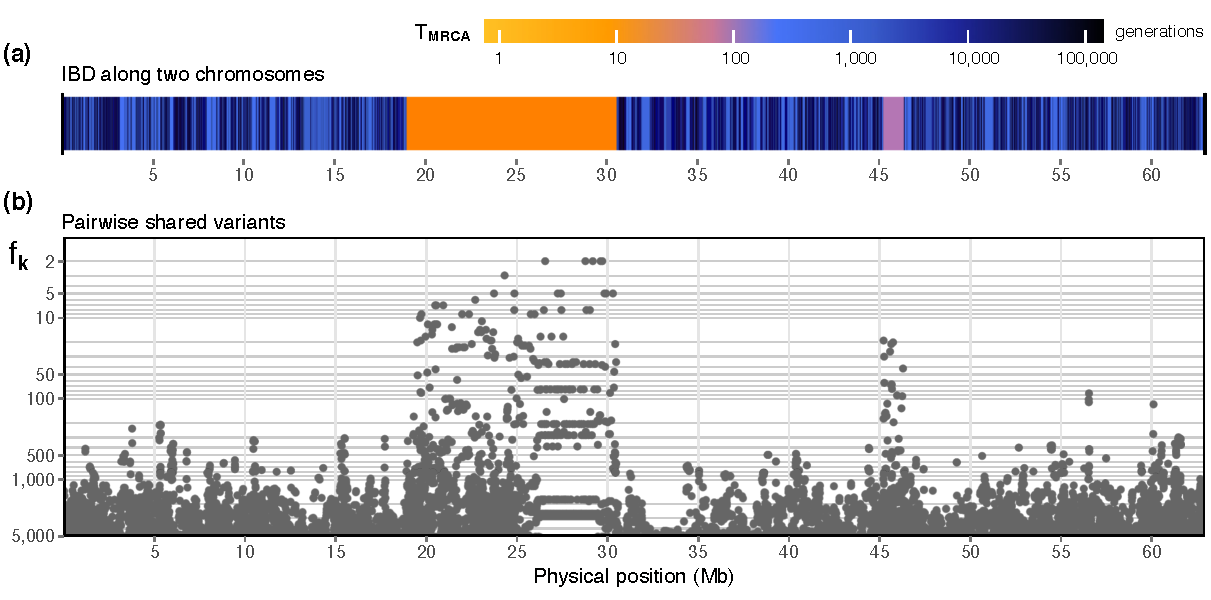
\includegraphics[width=\textwidth]{./img/ch3/pair_ibd_example}
\Caption{IBD structure and pairwise variant sharing}
{A dataset of ${N=\num{5000}}$ haplotypes was simulated under the coalescent using \texttt{msprime} \citep{Kelleher:2016fn}.
IBD status was determined from simulated genealogies for a pair of chromosomes selected at random from the set of chromosomes that shared a rare allele (frequency $\leq 0.5\%$).
Panel~\textbf{(a)} shows the ``mosaic'' of IBD segments along the full length of the simulated region for the \n{2} selected chromosomes.
The length of a given IBD segment is defined by the chromosomal interval over which the \gls{mrca} of the selected pair does not change.
The colour of each segment indicates the \gls{tmrca} for the selected pair.
Panel~\textbf{(b)} shows the physical position of \fk{} variants shared by the \n{2} chromosomes, ranging from very low allele frequency at the top (\fk{2}) to very high frequency at the bottom (\eg~\fk{>500}).
Note that the simulation was carried out under variable recombination rates using the genetic map for human chromosome~20 from the \glsentryfull{hapmap} Phase~\rom{2} Build~37.
The pattern of extended shared variation seen at positions around 25--30~\gls{Mb} arises from a low recombination rate at the region of the centromere.}
{fig:pair_ibd_example}
% \vspace{-5pt}
% \hrulefill%
\end{figure}

\glslocalresetall

%

Given this exponential ``decay'' of IBD length over time, rare or low-frequency variants are useful for identifying genomic regions in which individuals are likely to share recent and relatively long IBD tracts.
For example, \citet{Mathieson:2014ig} selected doubletons (alleles that are present only twice in a sample), which they refer to as \fk{2} variants, to identify the shared haplotype in the \n{2} individuals sharing the allele.
To borrow from this notation, henceforth, \fk{} is used to denote a variant at which $k$ allele copies are found in a sample.

To emphasise the utility of rare variants, see the example shown in \cpref{fig:pair_ibd_example}.
Using coalescent simulations, a sample of ${N = \num{5000}}$ chromosomes was generated.\footnote{See \cpref{sec:msprime} for a description of how data were simulated.}
A rare variant was randomly selected (frequency $\leq 0.5\%$), as well as \n{2} of the chromosomes which share the focal allele.
The underlying IBD structure for the given pair of chromosomes was determined from simulation records and shown in \cref{fig:pair_ibd_example}{a}.
IBD segments are distinguished by the \glsentryfull{tmrca} at each position along the sequence.
To illustrate pairwise allele sharing, \Correct{the} frequency of each allele shared by the \n{2} haplotypes is shown by chromosomal position in alignment with the IBD structure above; see \cref{fig:pair_ibd_example}{b}.
As suggested in the figure, the majority of low-frequency variants align with IBD segments that are more recent.

%
%!TEX root = ../../main.tex


\begin{figure}[p]
\makebox[\textwidth][c]{%
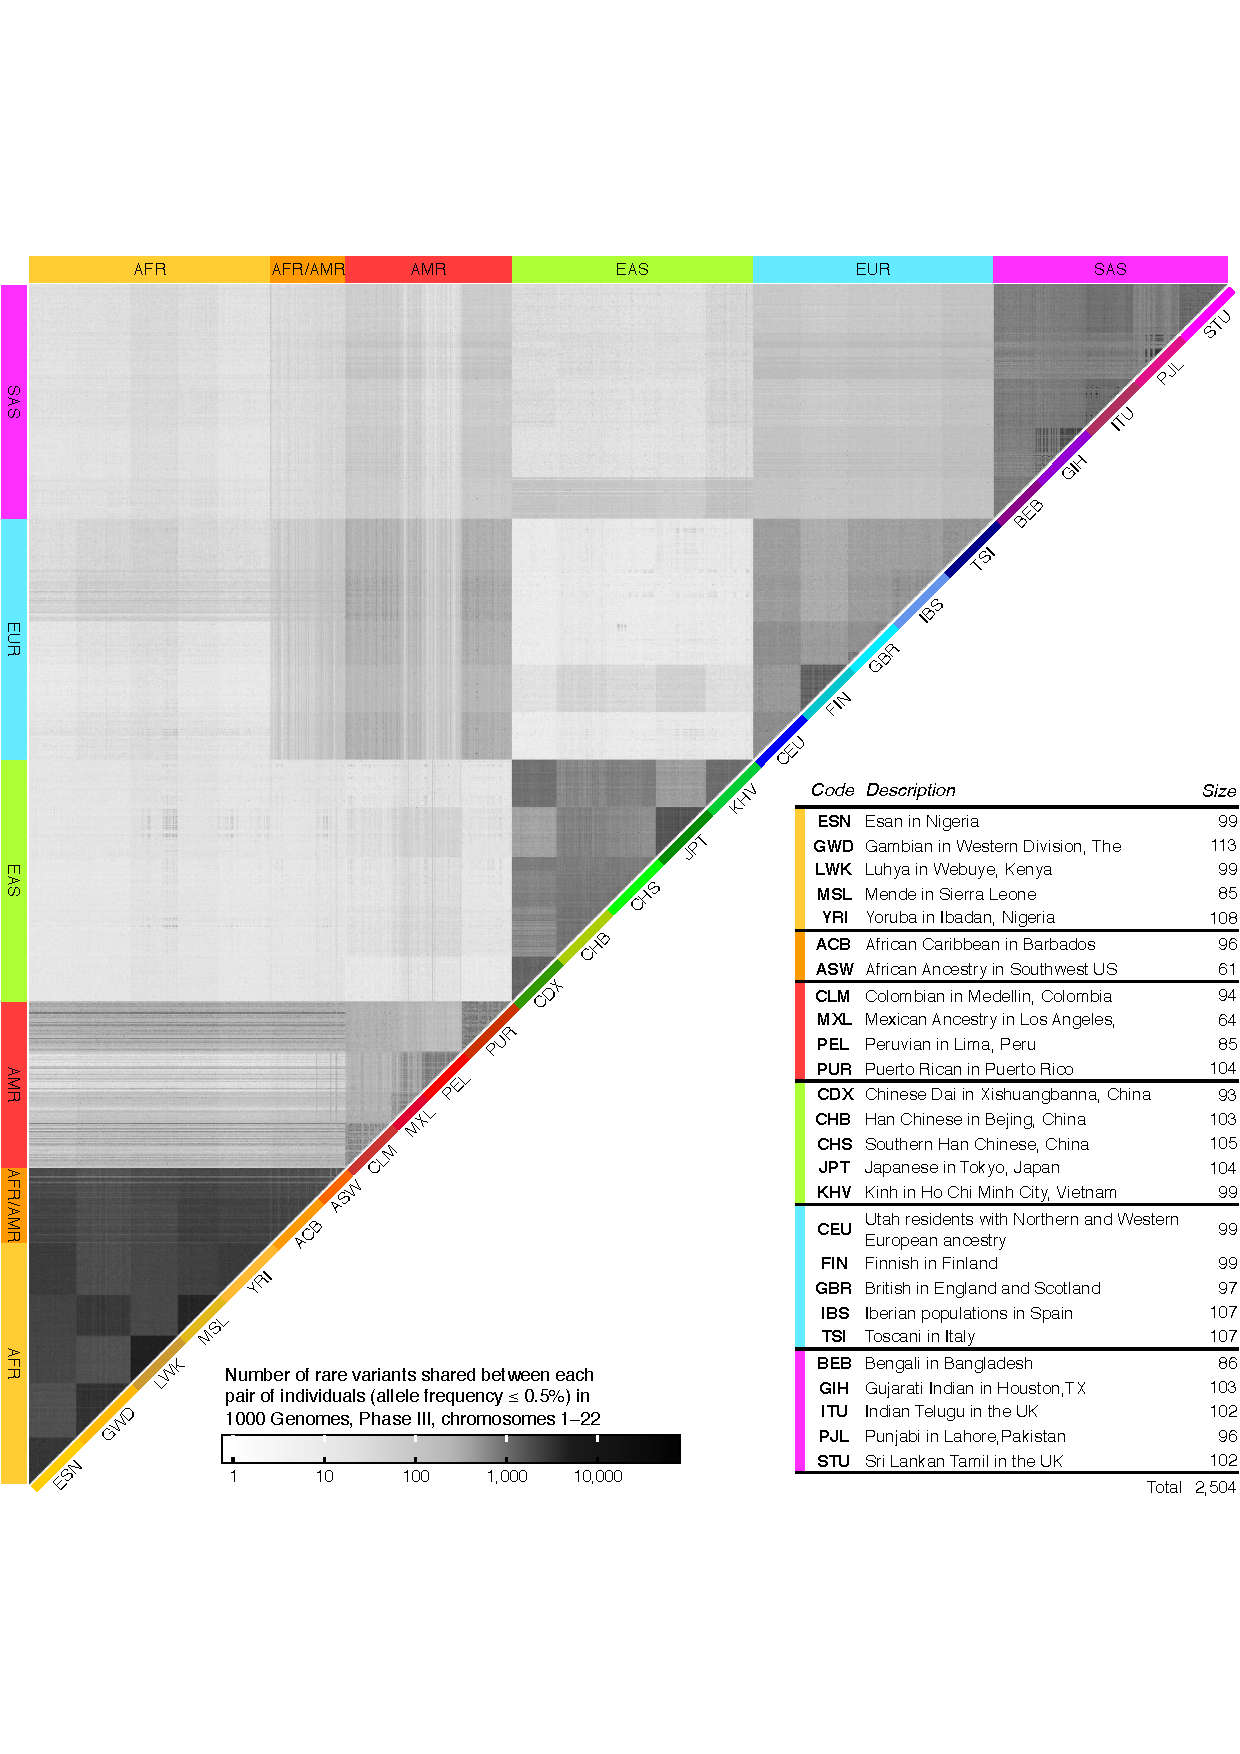
\includegraphics[width=1.1\textwidth]{./img/ch3/popstruct_1kg}%
}
\Caption{Rare variant sharing in the 1000 Genomes dataset}
{The plot shows the upper triangle of a pairwise sharing matrix in which the number of variants shared in each pair of individuals is indicated by tones of grey (log-scaled), ranging from \emph{light} (low number) to \emph{dark} (high number); see legend.
Pairwise rare variant sharing was determined for all shared alleles observed at  frequency ${\leq 0.5\%}$, across chromosomes 1--22, and in each pair of the \n{2504} individuals present in the final release dataset of the \glsentrylong{1kg} Phase~\rom{3}.
The dataset comprises sample data from \n{6} continental populations (or \emph{super-populations}) which are further subdivided in \n{26}~populations of different ethnic background.
Each group is abbreviated using a \n{3}-letter code.
The \n{6} continental populations are defined as follows;
African~(AFR), African-American~(AFR/AMR), American~(AMR), East~Asian~(EAS), European~(EUR), and South~Asian~(SAS).
The table in the lower right corner shows the code and description of each  population sample, as well as the number of individuals in each group.}
{fig:popstruct_1kg}
\end{figure}

%

The majority of variants observed in the human genome are low in frequency or rare.
For example, there are \Value{84.7}~million \glspl{snp} in the final release dataset of the \gls{1kg} Phase~\rom{3} (${N = \num{2504}}$), of which \Percent{71.93193} are below 1\% allele frequency and \Percent{64.2427} are below 0.5\% (after removing singletons and monomorphic sites), suggesting that there are ample opportunities to find rare allele sharing.
This is illustrated in \cpref{fig:popstruct_1kg}, which indicates the number of alleles shared between each pair in the dataset (chromosomes~1--22), at allele frequency~${\leq 0.5\%}$.
Notably, the sharing pattern highlights population structure, as the number of shared alleles is generally larger within a sub-population.



%
\section{IBD detection around rare variants}
\label{sec:tidy}
%

In the following sections, I describe the methodology by which IBD segments are detected around rare variant sites.
I then describe the implementation of each of the \n{2} tests for the detection of IBD segments in large sample data.
Lastly, I conclude this section by highlighting certain caveats of the implemented method before its evaluation using simulated data.


%
\subsection{Inference of historical recombination events}
%

\N{2} approaches for a non-probabilistic inference of recombination events are described below; these are the \emph{\acrlong{fgt}} \citep{Hudson:1985wh}, which requires haplotype information, and the criterion of \emph{inconsistent homozygote genotypes} \citep[see][]{Mathieson:2014ig}, which requires genotype data; henceforth referred to as the \emph{\acrlong{dgt}}.

\Addition{Note that the aim of this implementation is to detect recombination in pairs of diploid individuals, relative to a given target position in the genome, where it is attempted to delimit the shared haplotype segment of the two haplotypes sharing the target allele.
This is further explained in \cpref{sec:ibd_detect_alg}, with examples provided in \cpref{sec:ibd_detect_lim}.}


\paragraph{\Gls{fgt}.}
Given \n{4} haplotypes in \n{2} diploid individuals, a recombination event is inferred between \n{2} loci if all \n{4} possible gametes are observed.
This holds true under the infinite sites model \citep{Kimura:1969tn}, where mutation events may only occur once per site in the history of a sample, such that at most \n{2} allelic states can be observed at a given site.
It follows that for a pair of sites there are \n{4} possible allelic state configurations; ${(0,0)}$, ${(0,1)}$, ${(1,0)}$, and ${(1,1)}$, where 0 and 1 denote the ancestral and derived type, respectively.
If all \n{4} configurations are observed, genealogies at the \n{2} sites are incompatible and the observation can only be explained by a recombination event that occurred in the history of the sample.
Because recurring mutations or back mutations are assumed to have zero probability, at least \n{1} recombination event must have occurred in the interval between the \n{2} sites.
In the following, the term \emph{breakpoint} is used for either of the \n{2} sites that together delimit the interval.
An example configuration is shown in \cpref{fig:info_fgt}.

%
%!TEX root = ../../main.tex


\begin{figure}[!htb]
\centering
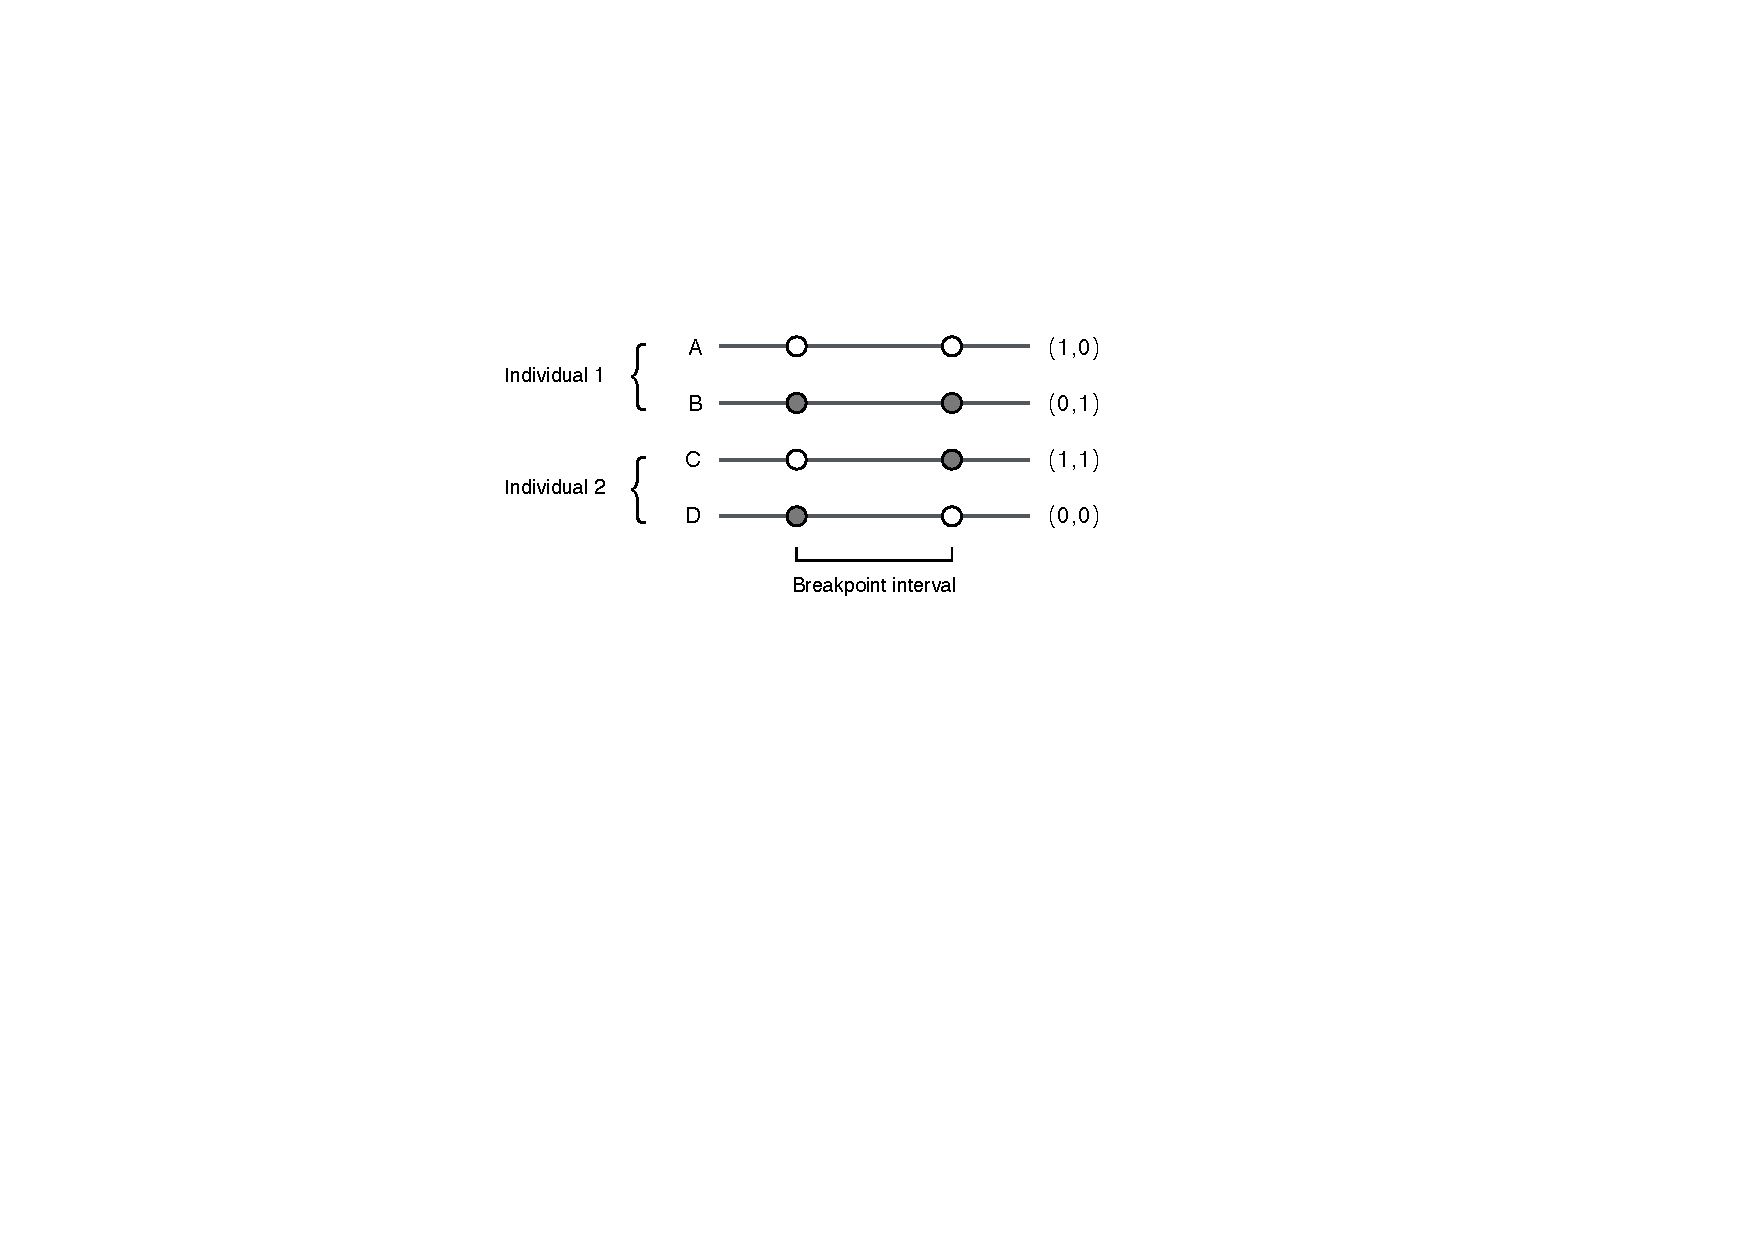
\includegraphics[width=0.7\textwidth]{./img/ch3/info_fgt}
\Caption{Breakpoint detection using the four-gamete test (FGT)}
{The \n{4} haplotypes (gametes) in a pair of \n{2} diploid individuals are shown (\emph{horizontal lines}).
A breakpoint interval is detected if all \n{4} possible allelic state configurations are observed at \n{2} variant sites along the sequence.
The interval delimits the region in which at least \n{1} recombination event must have occurred in the history of the sample (given the assumptions of the infinite sites model).
The \n{4} allelic state configurations are shown on the \emph{right}.
The alleles are shown at the \n{2} breakpoint sites; indicated as ancestral (\emph{hollow} circle) and derived state (\emph{solid}).
Note that the order of gametes is ignored.}
{fig:info_fgt}
\end{figure}

%

Notably, private or \emph{de~novo} mutations appearing as singletons in the sample cannot lead to the observation of the \n{4} required configurations.
Although the exact location of recombination (\ie chromosomal crossover) cannot be retrieved from the data, the \gls{fgt} can be used to find the smallest interval in which at least \n{1} recombination event occurred.
\Addition{However, it is important to note that this test cannot determine which of the four haplotypes recombined, and where it is also possible that there have been multiple recombination events pertaining to different haplotypes within the detected interval.}


\paragraph{\Gls{dgt}.}
In absence of haplotype information, data are represented as genotypes, where genotypic states are encoded as 0, 1, and 2, for variants that are homozygous for the ancestral allele, heterozygous, and homozygous for the derived allele, respectively.
Given the genotype sequences of \n{2} diploid individuals, recombination is inferred between \n{2} sites; one being heterozygous in both individuals (\ie the genotypes 1 and 1) and another with opposite homozygous genotypes (0 and 2).
In the latter case, it follows that the \n{2} individuals cannot share a haplotype at that locus.

The \gls{dgt} is a special case of the \gls{fgt}, as the same composition of alleles is implied.
For example, if the allelic configurations ${(0,1)}$ and ${(0,0)}$ are seen in individual~1, and configurations ${(1,0)}$ and ${(1,1)}$ in individual~2, the corresponding genotypic configurations are ${(0,1)}$ and ${(2,1)}$, respectively, which satisfies the breakpoint condition in both the \gls{fgt} and \gls{dgt}.
However, because genotype data result from haplotype occurrence in individuals, not all breakpoints detectable under the \gls{fgt} can be found using the \gls{dgt}.
At sites where the \gls{fgt} detects a breakpoint interval, the \gls{dgt} cannot break if both sites are heterozygous in the same individual.
As a consequence, it can be expected that the \gls{dgt} is more restrictive than the \gls{fgt}; \eg if breakpoints are found, they are likely to sit farther apart.

%
%!TEX root = ../../main.tex


\begin{figure}[!htb]
\centering
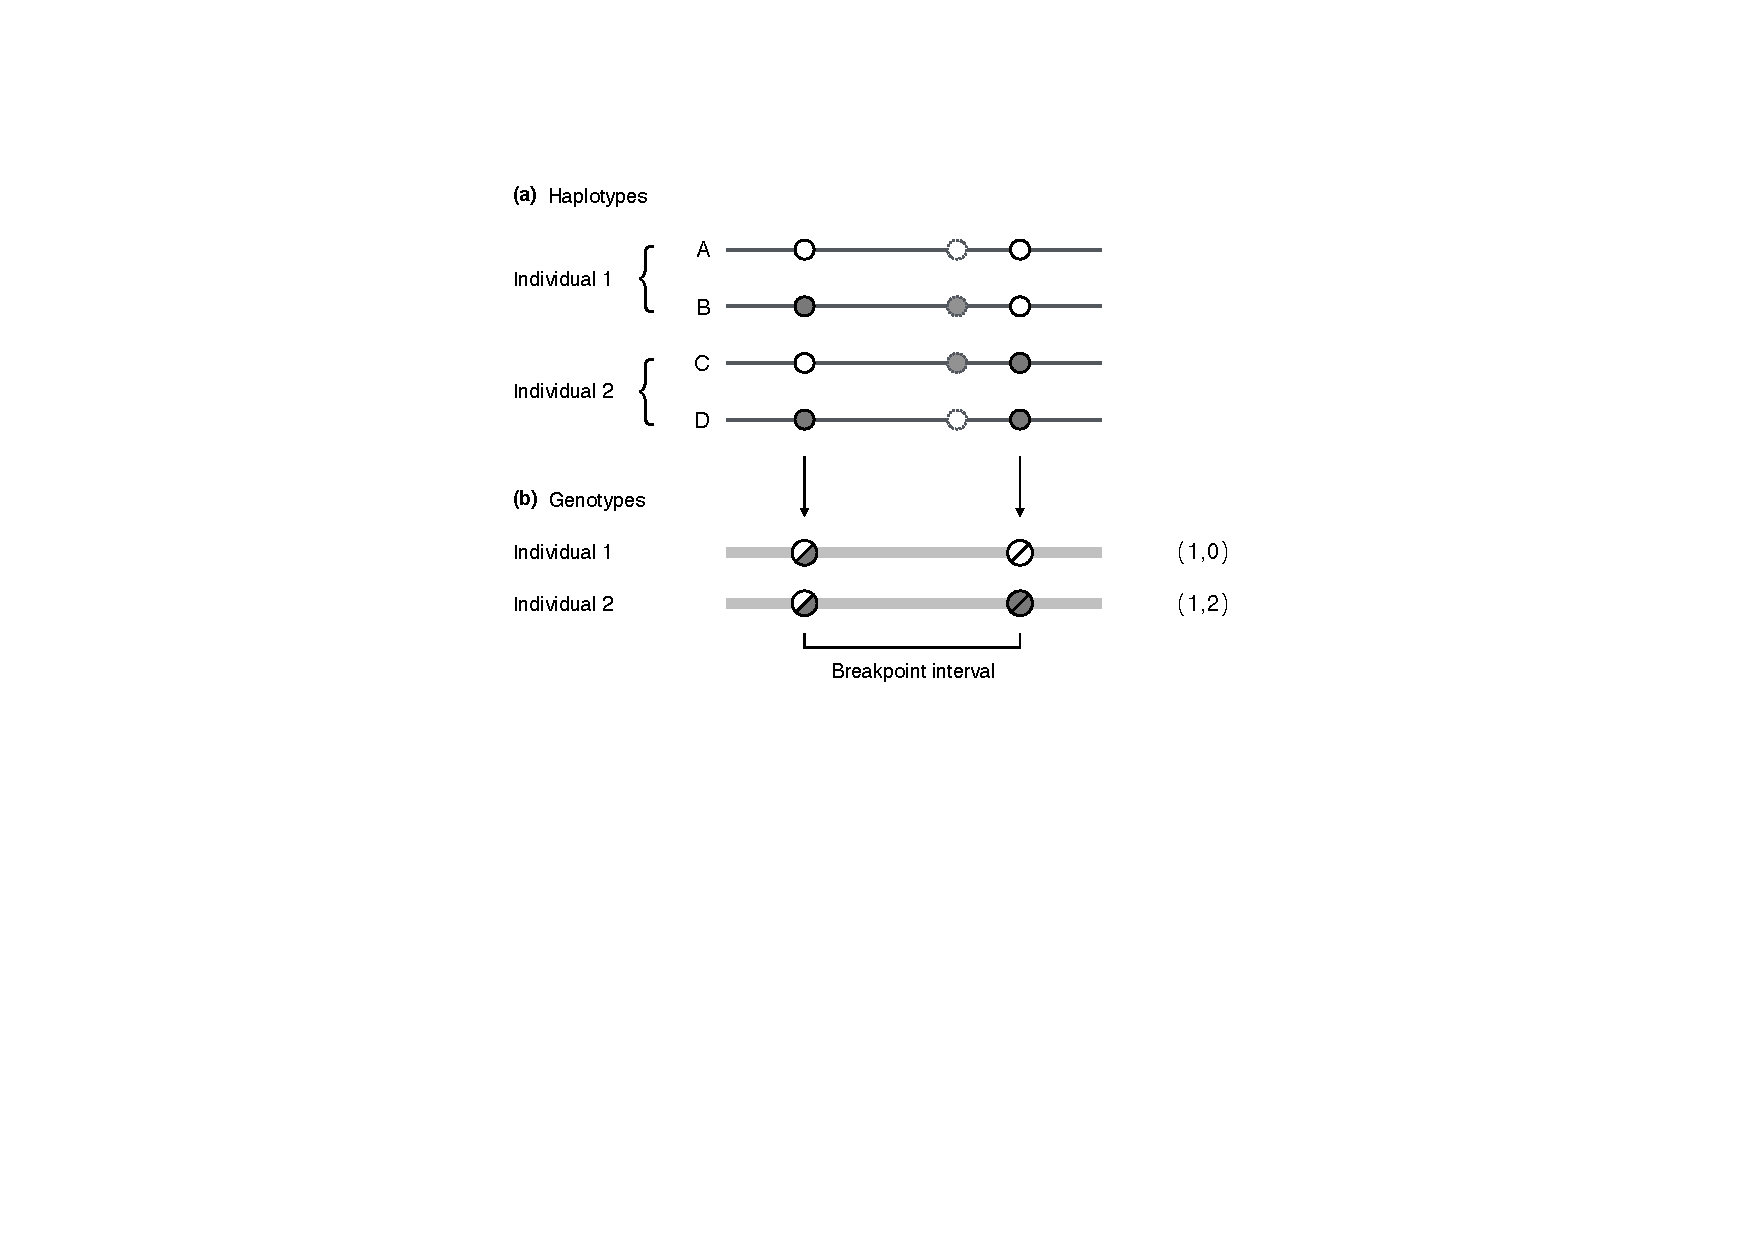
\includegraphics[width=0.7\textwidth]{./img/ch3/info_dgt}
\Caption{Breakpoint detection using the discordant genotype test (DGT)}
{Unlike the \gls{fgt}, which requires haplotype information, the \gls{dgt} identifies a breakpoint interval using genotype data.
For comparison, Panel~\textbf{(a)} shows the \n{4} gametes of the \n{2} individuals involved; see \cpref{fig:info_fgt}.
To highlight the difference to the \gls{fgt}, an additional variant is shown in between both sites; alleles indicated by a \emph{dotted} edge.
This site would satisfy the breakpoint condition under the \gls{fgt}, but is missed under the \gls{dgt}.
Panel~\textbf{(b)} shows the \n{2} genotype sequences per individual (\emph{thick} horizontal lines) from which a breakpoint interval is inferred using the \gls{dgt}.
The genotypic states of the breakpoint sites are given on the \emph{right}.
Genotypes can either be homozygous for the ancestral allele (\emph{hollow} circle), heterozygous (\emph{semi-solid}), or homozygous for the derived allele (\emph{solid}).}
{fig:info_dgt}
\end{figure}

%

\Addition{The \gls{dgt} thereby simplifies the breakpoint condition to observing opposite homozygote genotypes in two diploid individuals, but where allele sharing at a given target site (that is heterozygous in both individuals) is required such that the conditions of the \gls{fgt} would be satisfied.}
This is further exemplified in \cpref{fig:info_dgt}, which highlights the difference to the \gls{fgt} by comparison to the example shown in \cpref{fig:info_fgt}.


%
\subsection{Description of the algorithm}\label{sec:ibd_detect_alg}
%

The \gls{fgt} and \gls{dgt} provide the means for non-probabilistic inference of recombination breakpoints from either haplotype or genotype data, respectively.
This methodology is implemented such that the full length of an IBD segment can be found around a given target site in a pair of diploid individuals.
The allele at a target site serves as an indicator for haplotype sharing by descent; hence, to detect recent IBD, rare variants are used as primary targets.
The aim of this method is to infer breakpoint intervals independently on both sides of the target position along the sequence, so as to infer the \n{2} recombination events that delimit the underlying IBD segment.
As such, the target variant is set as the \emph{focal} breakpoint.
The algorithm is described below; a more intuitive example is illustrated in \cpref{fig:info_breakpoint}.

%
%!TEX root = ../../main.tex


\begin{figure}[!tbp]
\centering
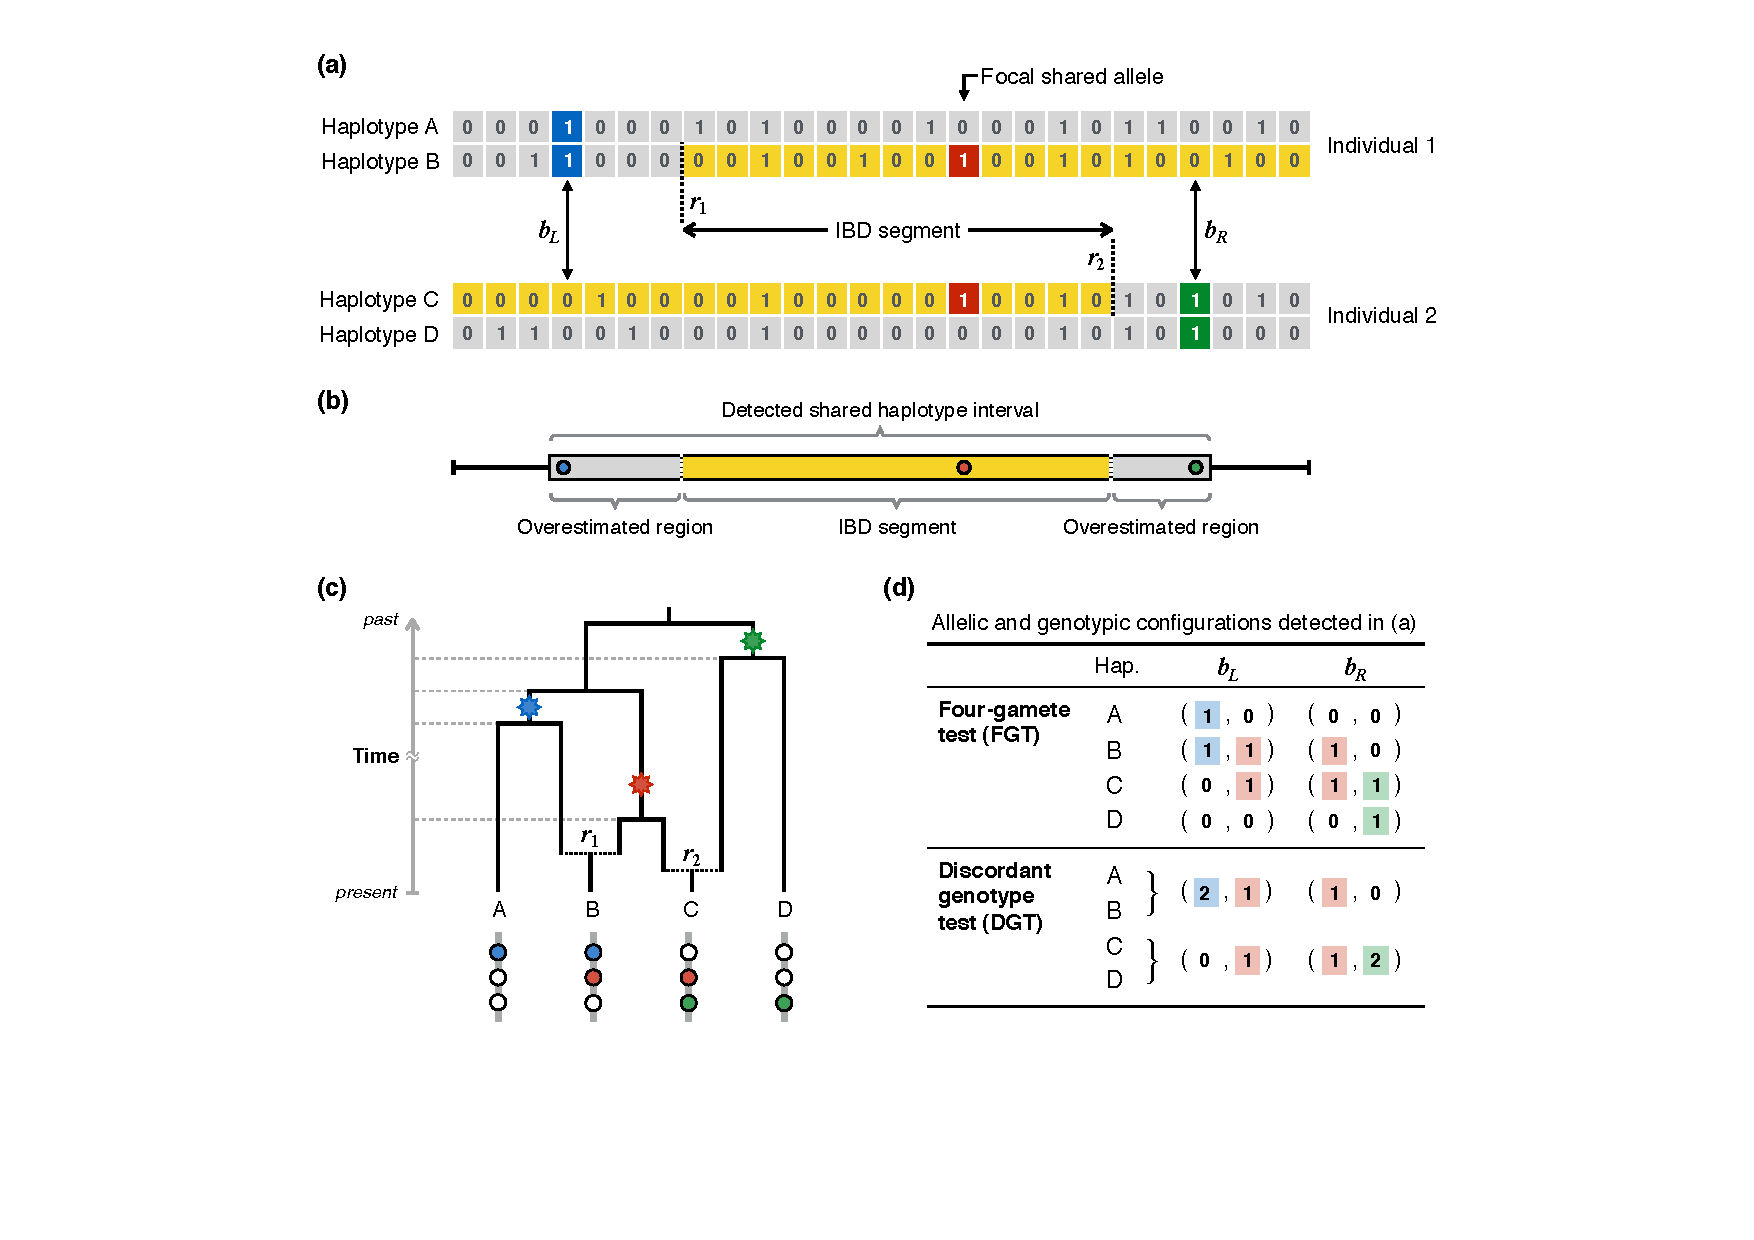
\includegraphics[width=\textwidth]{./img/ch3/info_breakpoint}
\Caption{Illustration of shared haplotype detection in a pair of diploid individuals}
{Panel~\textbf{(a)} shows \n{2} individuals composed of haplotypes A and B, and haplotypes C and D, respectively.
Each haplotype is represented as a sequence of observed allelic states, where $0$ and $1$ denote the ancestral and derived allele, respectively.
Breakpoints are detected by independently scanning to the left and right-hand side from the target position.
The \n{2} individuals share a haplotype by descent (highlighted in \emph{yellow}) which is tagged by the focal allele (\emph{red}), for which the \n{2} individuals are heterozygous
\N{2} sites (\emph{blue} and \emph{green}) mark the first sites at which a breakpoint condition is satisfied, such that $b_{L}$ and $b_{R}$ are detected.
The IBD segment shared by both individuals is indicated by $r_{1}$ and $r_{2}$ (\emph{dashed lines}).
Panel~\textbf{(b)} shows the detected breakpoint interval, delimited by $b_{L}$ and $b_{R}$ (inclusive).
Note that detected breakpoints are only the first indication of recombination found distal to the focal site, but may not mark the points of the actual crossover events; thus, it is expected that the length of the detected segment is overestimated, dependent on available data.
Panel~\textbf{(c)} represents the history of the sample as an \gls{arg}.
Mutation events are indicated on the tree (\emph{stars}) and gave rise to the alleles highlighted in~(a); \emph{blue}, \emph{red}, and \emph{green}.
The dotted \emph{grey} lines indicate the time of coalescent events in the history of the sample; dotted \emph{black} lines indicate recombination events.
Panel~\textbf{(d)} provides a table outlining the configurations of allelic and genotypic states at breakpoint sites as considered in the \gls{fgt} and \gls{dgt}, respectively.
Notably, in the example shown, both the \gls{fgt} and \gls{dgt} detect breakpoints at indicated sites.
But, for example, if individual~1 was composed of haplotypes A and C, and individual~2 of haplotypes B and D, the breakpoints would be detected as shown under the \gls{fgt}, but not the \gls{dgt}.}
{fig:info_breakpoint}
\end{figure}

%

Let $M$ be the number of variant sites observed in a sample of $N$ diploid individuals.
At the target site, $b_{i}$, where ${i \in \lbrace 1, 2, \ldots, M \rbrace}$, the subset of individuals sharing the derived allele is identified and compared in a pairwise fashion.
Importantly, the allele at this site is used as an identifier for haplotype sharing, on which inference is conditioned in either the \gls{fgt} or \gls{dgt}.
Thus, individuals are only considered if they are heterozygous for the focal allele, as the breakpoint condition in either test cannot be satisfied otherwise.
However, note that this restriction arises from the variant-centric focus on a given rare allele; \eg the condition of the \gls{fgt} could be satisfied for individuals homozygous for a given allele, but without that the allele is shared by the other individual (hence, defying the purpose of this implementation).
In each pair, chromosomes are scanned to the left and right-hand side from the target site until the first site is found that, together with the allelic or genotypic states observed at $b_{i}$, satisfies the breakpoint condition, which is done independently on each side.
Detected breakpoints are labelled as $b_{L}$ and $b_{R}$ on the left and right-hand side, respectively, such that the intervals ${[b_{L}, b_{i}]}$ and ${[b_{i}, b_{R}]}$ delimit the chromosomal regions in which recombination events occurred, respectively; where ${L,R \in \lbrace 1, 2, \ldots, M \rbrace}$.
Hence, the underlying IBD segment is enclosed in ${[b_{L}, b_{R}]}$.

The allelic or genotypic states at $b_{L}$ or $b_{R}$ provide only the first indication of recombination found along the sequence on either side of the focal allele, but may not mark the points of the actual crossover events.
The detected interval is therefore inclusive of the breakpoints such that the full length of the underlying IBD segment is covered.
%However, this is expected to lead to an overestimation of the shared haplotype length.
In cases where the end of a chromosome is reached without detecting any evidence of recombination, the terminal site is recorded to capture the length of the segment; this is hereafter referred to as a \emph{boundary case}.



%
\subsection{Anticipated limitations}\label{sec:ibd_detect_lim}
%

As noted by \citet{Hudson:1985wh}, not all recombination events in the history of a sample are found by the \gls{fgt}, and are therefore also missed by the \gls{dgt}.
In the implementation presented, a breakpoint is found by performing a scan along the sequence away from a target position.
Provided that the neighbouring haplotype regions derive from different ancestral lineages, in the general case, it is likely that a breakpoint will be found eventually (or the boundary of the chromosome is reached).

The main limitation to the accuracy of the detected breakpoints is the overestimation of the interval, in relation to the underlying true IBD length; as shown in \cref{fig:info_breakpoint}{b}.
While the underlying IBD segment is enclosed in the interval, it can be expected that breakpoints are detected at sites some distance away from where recombination occurred, thus overestimating the true length of the underlying IBD tract.
The extent of overestimation is dependent on the number and density of observed variant sites in the sample.
Because the rate of mutation is directly proportional to the expected number of segregating sites \citep{Watterson:1975ur}, a higher mutation rate can generally be expected to decrease the overestimation of segment length.

\Correct{When using \gls{wgs} data, strategies for variant calling and filtering may affect the accuracy of detecting recombination events as not all variant sites might be captured correctly.
It cannot be expected that genotyping arrays provide sufficient marker density to infer breakpoints with high accuracy (with regard to the true length of the underlying shared haplotype segment).}


%
%!TEX root = ../../main.tex


\begin{figure}[!htbp]
	% {\scriptsize \texthv{\textbf{(a)} Example 1}} \\
	% 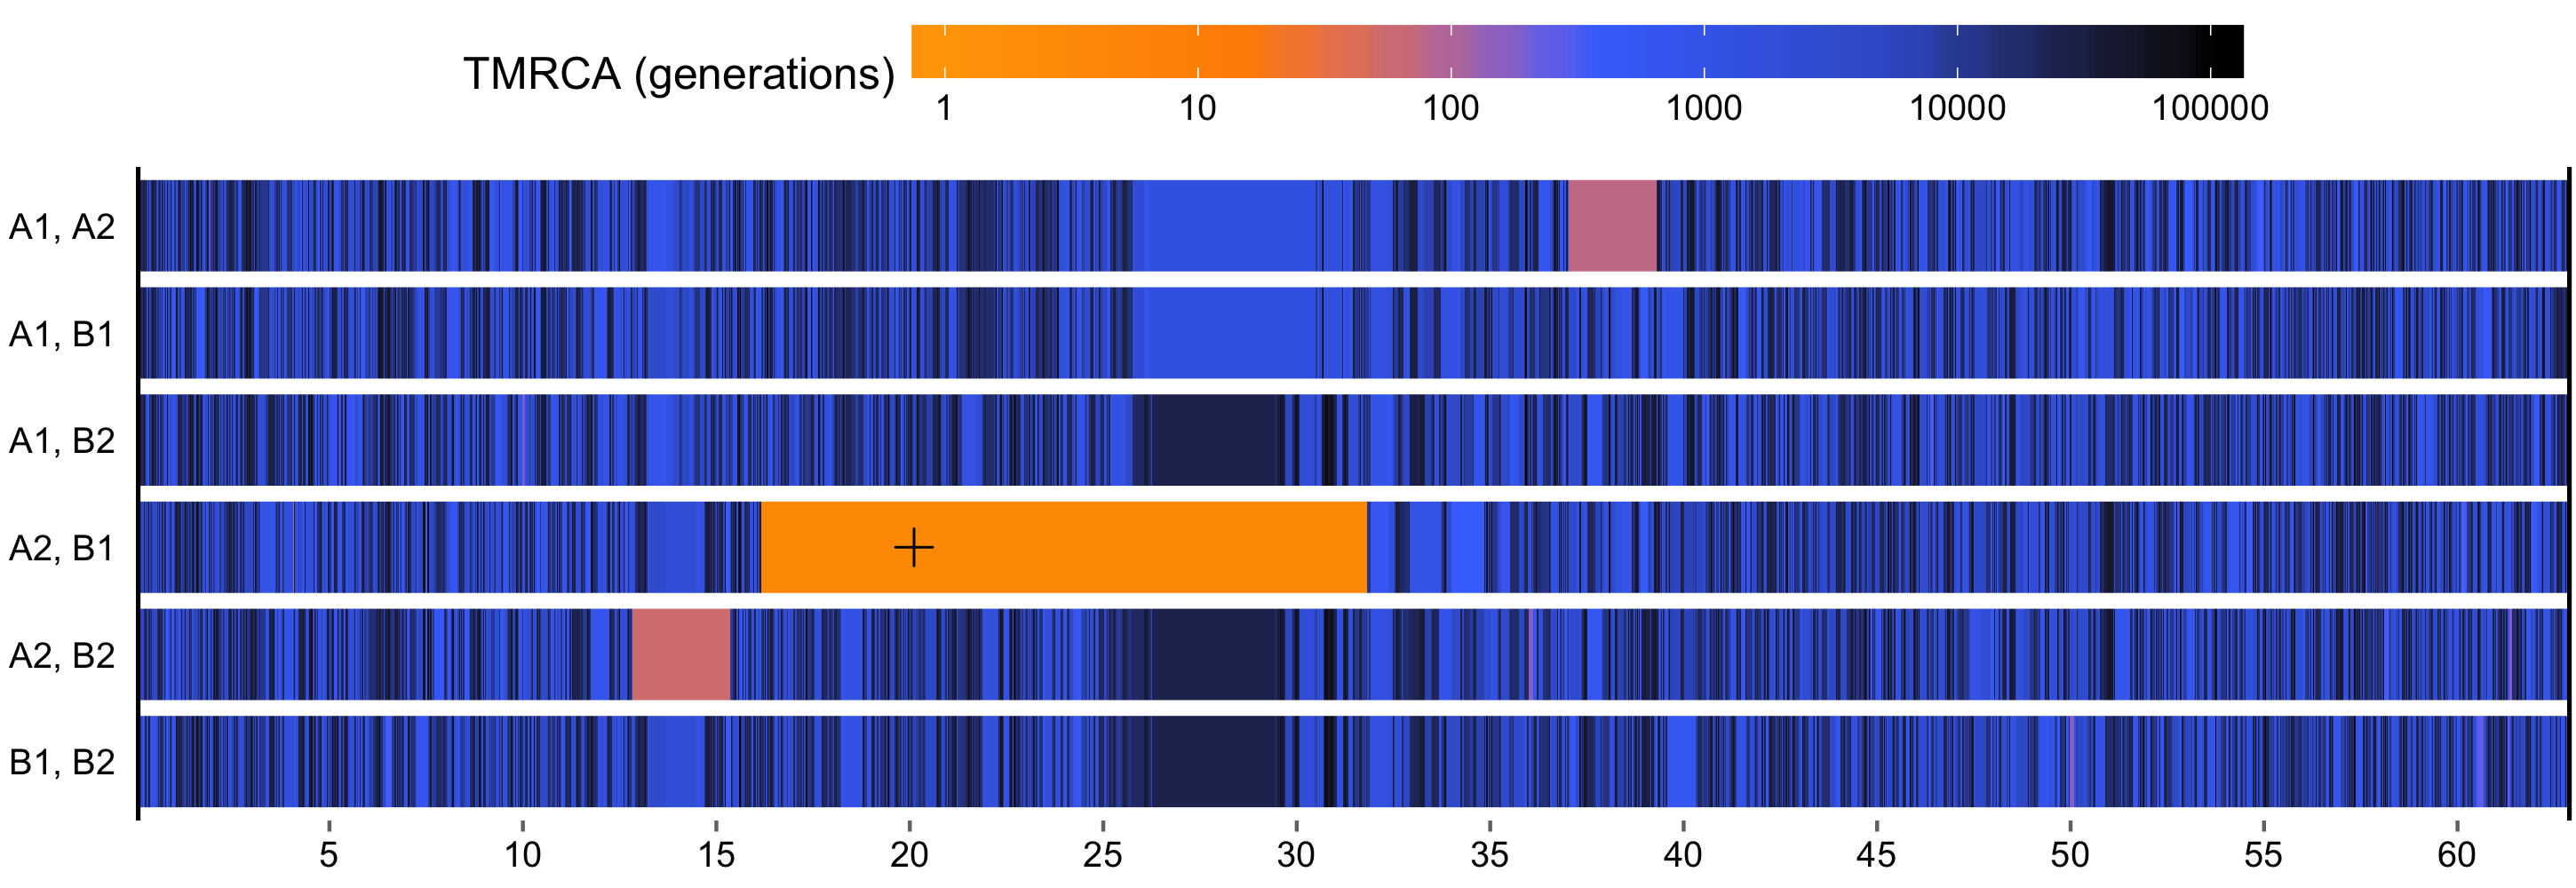
\includegraphics[width=\textwidth]{./img/ch3/full_ibd_example_A.png}
	% 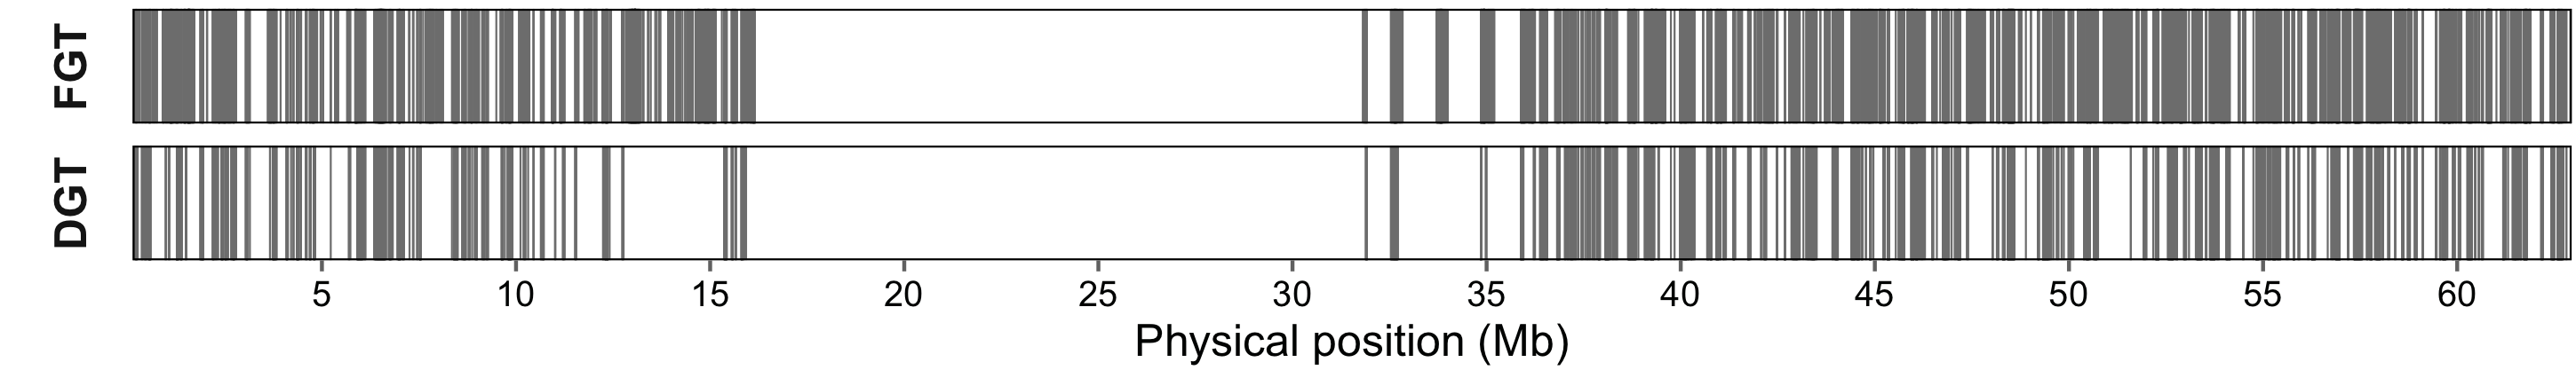
\includegraphics[width=\textwidth]{./img/ch3/full_ibd_example_B.png}
	% {\scriptsize \texthv{\textbf{(b)} Example 2}} \\
	% 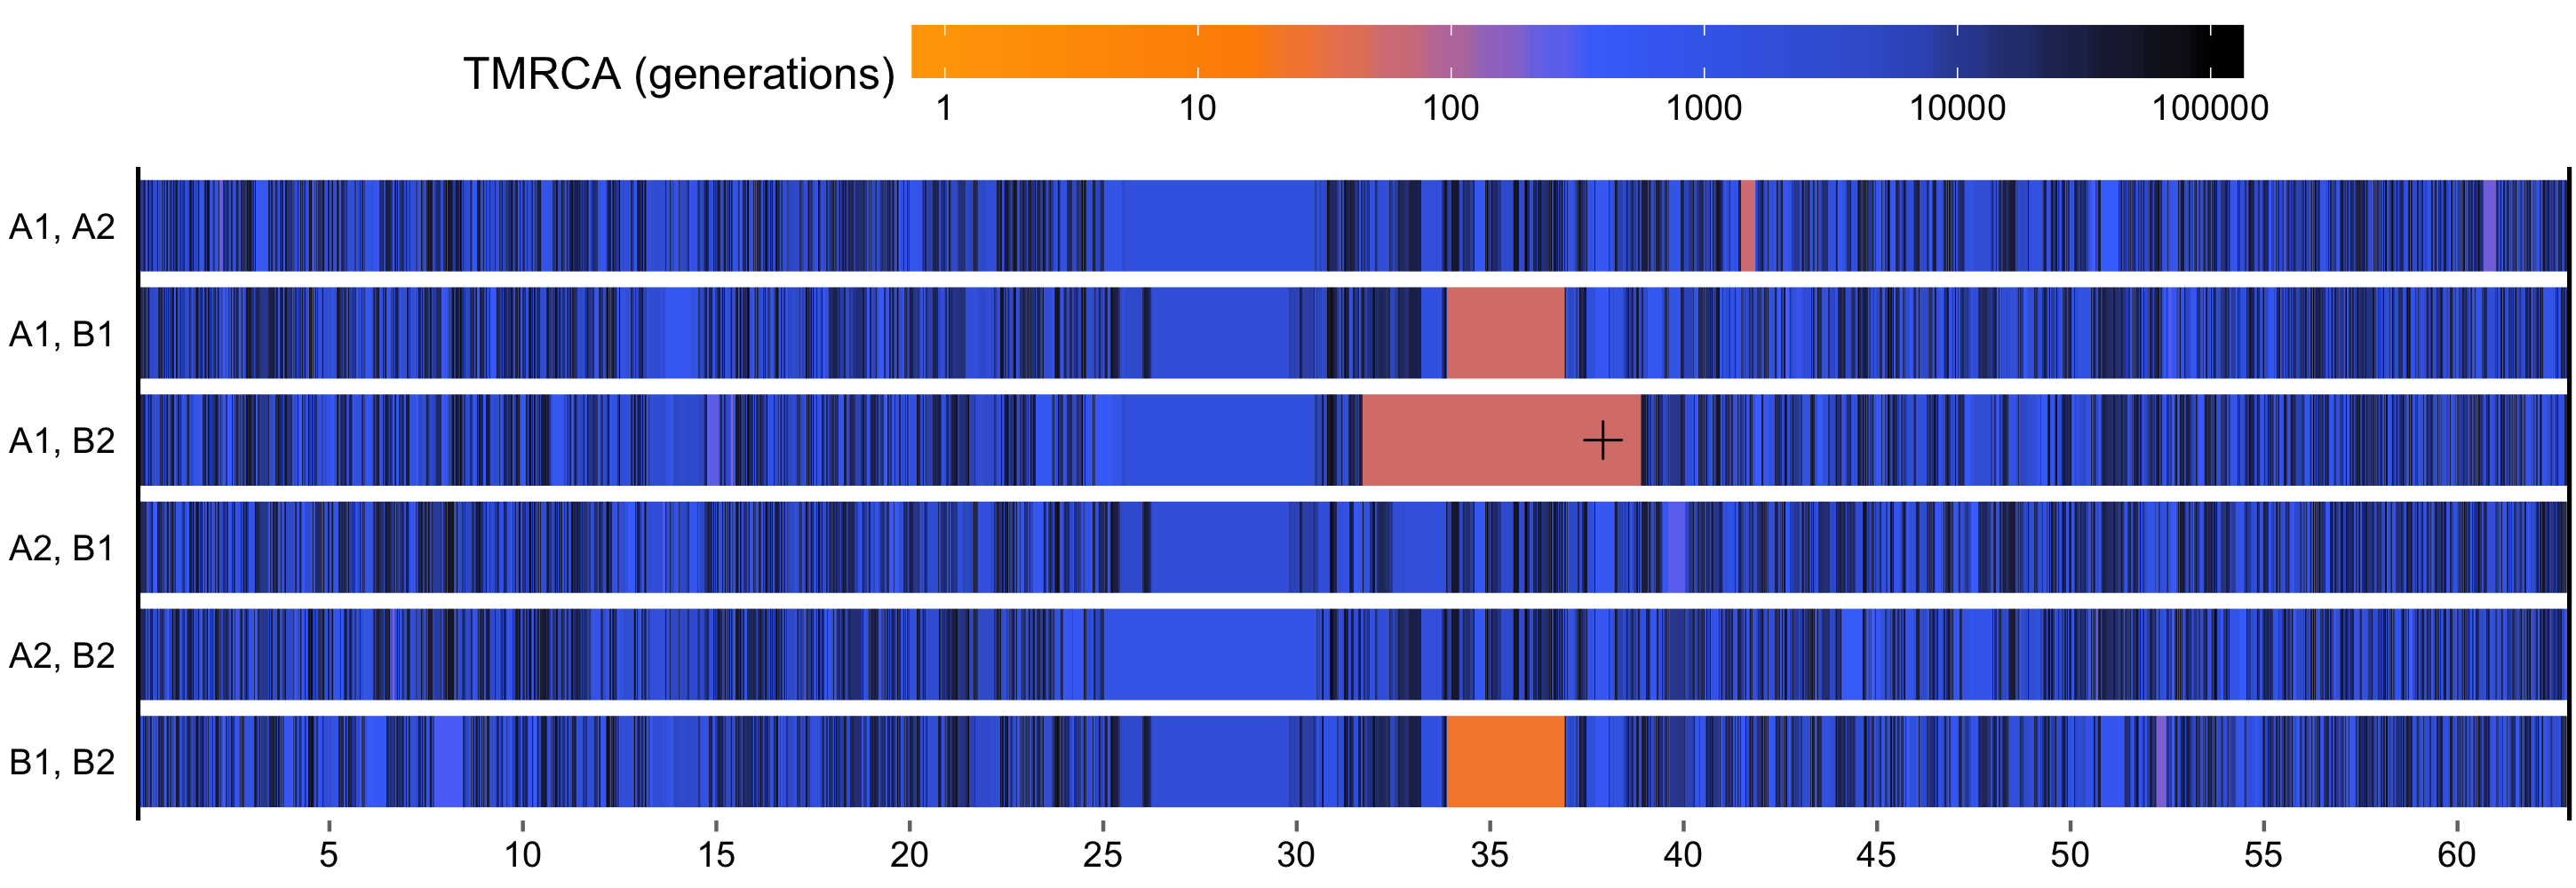
\includegraphics[width=\textwidth]{./img/ch3/full_ibd_underest_A.png}
	% 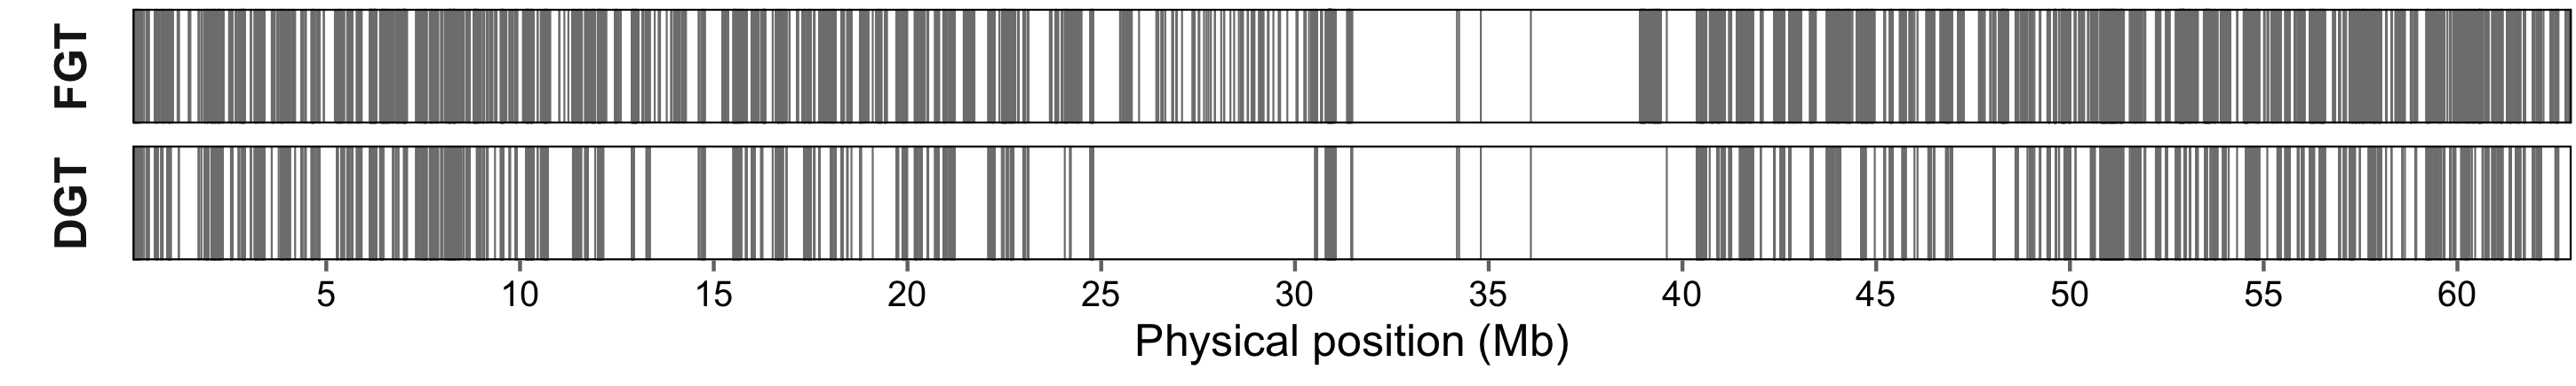
\includegraphics[width=\textwidth]{./img/ch3/full_ibd_underest_B.png}
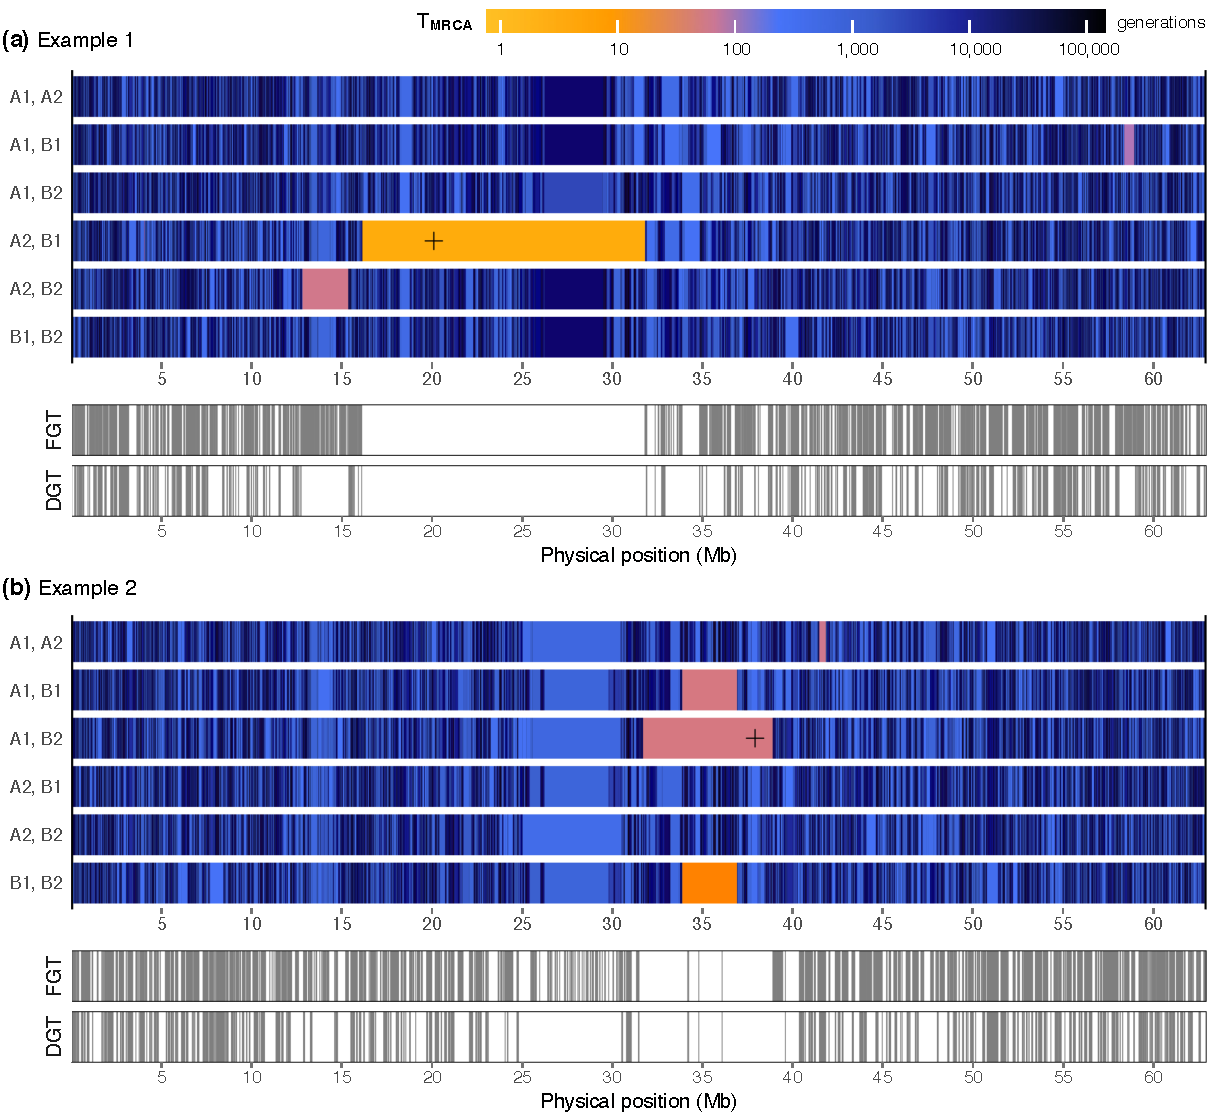
\includegraphics[width=\textwidth]{./img/ch3/full_ibd_example}
\Caption{Examples of the underlying IBD structure in each pair of four chromosomes}
{The true, underlying IBD structure is shown for each possible pair among \n{4} chromosomes in \n{2} diploid individuals; \n{2} examples are shown.
Each chromosome is labelled by its occurrence in individuals A~and~B, where chromosomes~1~and~2 are distinguished.
The ``mosaic'' of IBD segments per pair was determined from coalescent records produced in simulations using \texttt{msprime} \citep{Kelleher:2016fn}; see \cpref{sec:msprime}.
Each segment defines the region that was co-inherited from a \gls{mrca}, and is colour-coded by the number of generations separating the \n{2} chromosomes from their shared \gls{mrca} in that region.
The \emph{cross} marks the position of the focal allele in the pair that shares it.
Below, all breakpoints detected relative to the focal variant along the simulated region are indicated, using the \gls{fgt} (\emph{top}) and \gls{dgt} (\emph{bottom}).
Panel~\textbf{(a)} shows that the innermost breakpoint intervals (relative to the target position) detected in the \gls{fgt} or \gls{dgt} align closely with the true termini of the IBD segment.
The extent of overestimation appears to be negligible in relation to the length of the detected segment.
Panel~\textbf{(b)} shows that the innermost intervals are underestimated, due to an overlap of recently co-inherited haplotypes on different chromosome pairs.}
{fig:full_ibd_example}
\end{figure}

%

Conversely, it is also possible that segment length is underestimated.
\Correct{A recombination event can occur with chromosomes outside the sub-tree of the lineages deriving from the focal mutation, such that a detected breakpoint may pertain to recombination occurring on either of the ``unshared'' haplotypes.}
Given the \n{4} chromosomes required, there are ${{{4}\choose{2}}=6}$ possible pairs of chromosomes which may share extended haplotype regions by descent.
\Correct{A segment that was more recently co-inherited by one of the two other haplotypes that do not share the focal allele may result in detection of an ``unwanted'' breakpoint, where recombination did not break the genealogical relationship between the haplotypes sharing the allele.
The \gls{fgt} or \gls{dgt} may correctly infer a recombination event, but which would result in an underestimation of the length of the focal IBD segment.}
This is illustrated in \cpref{fig:full_ibd_example}, which shows \n{2} examples generated using coalescent simulations.

In Example~1 (\ref{fig:full_ibd_example}{a}), a rare allele target site was randomly selected, as well as the \n{2} individuals sharing the \Correct{focal} allele.
The true IBD structure was determined from simulation records for each pair of the \n{4} chromosomes in the \n{2} individuals.
Each pair is represented by a mosaic of IBD segments along the sequence, where each segment is distinguished by \gls{tmrca}.
Both the \gls{fgt} and \gls{dgt} were applied, but where all consecutive breakpoints after the first detection were also recorded along the sequence on both sides of the focal variant.
The innermost interval delimits the detected shared haplotype segment around the target site.
Example~1 illustrates the case in which a rare allele identifies the underlying co-inherited haplotype segment, which may stand out as being much younger due to recent shared ancestry.

%
%!TEX root = ../../main.tex


\begin{figure}[!htb]
\centering
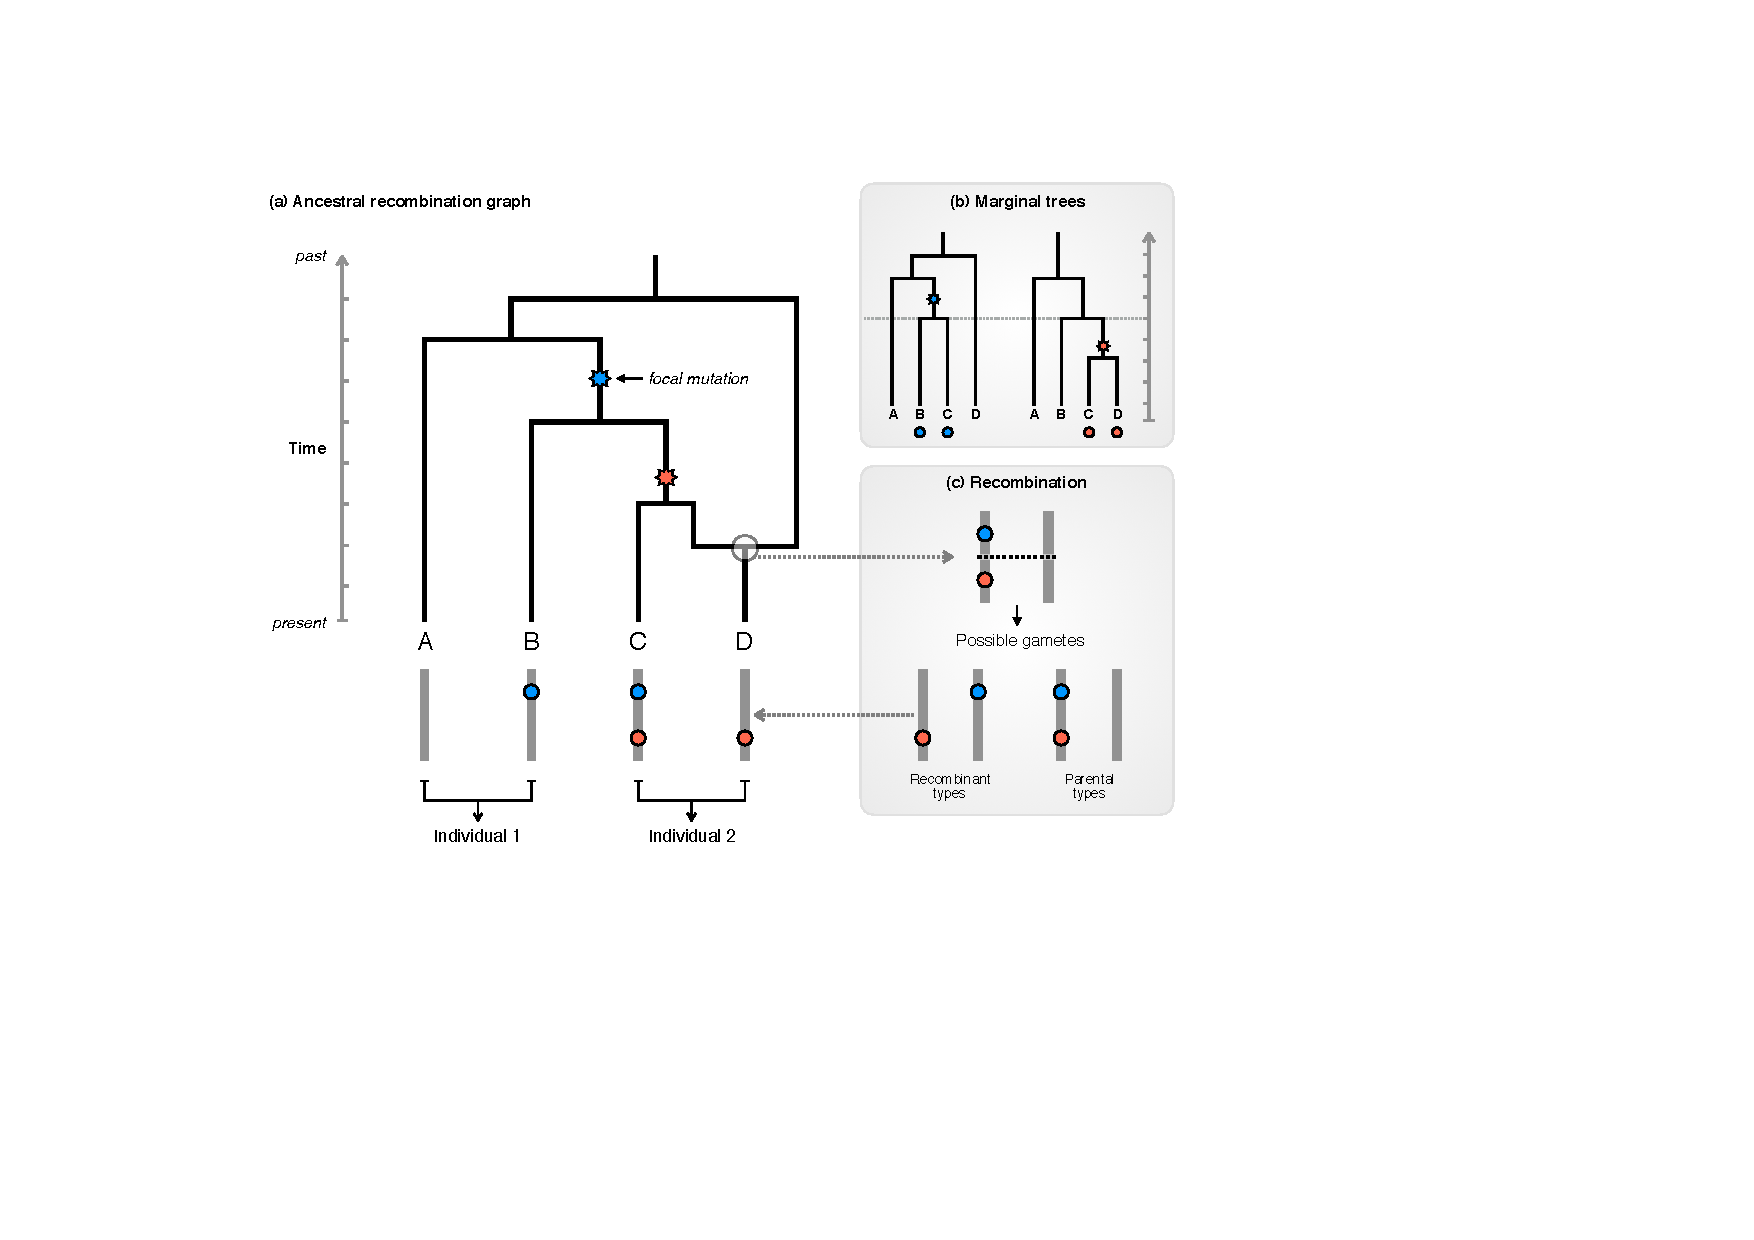
\includegraphics[width=0.9\textwidth]{./img/ch3/info_testfail_example}
\Caption{Recombination outside the focal sub-tree}
{The example shows \n{2} diploid individuals that share a focal allele (\emph{blue}) on haplotypes $B$ and $C$, which form a sub-tree within the larger genealogy.
Panel~\textbf{(a)} shows the \glsentryfull{arg} of a possible recombination history that would result in an ``unwanted'' detection of a breakpoint, due to recombination event outside the focal sub-tree.
Both the \gls{fgt} and \gls{dgt} would correctly detect a recombination event between the \n{2} sites.
However, because recombination occurred neither with haplotype $B$ nor $C$, the co-inheritance relationship between both haplotypes (relative to the focal allele) remained unbroken.
Panel~\textbf{(b)} shows the marginal trees at the \n{2} sites, corresponding to the \gls{arg} shown in Panel~(a).
Note that the \gls{tmrca} of haplotypes $B$ and $C$ in both marginal trees is identical.
Panel~\textbf{(c)} shows the possible gametes that can result from a recombination occurring between the \n{2} sites indicated.\AdditionLabel}
{fig:info_testfail_example}
\end{figure}

%

The same was done in Example~2 (\ref{fig:full_ibd_example}{b}), but here the target site and the pair of individuals was chosen because it was found that the length of the detected IBD segment was underestimated.
As can be seen, this underestimation is due to \Correct{a recombination event on an ``unshared'' haplotype (which does not carry the focal allele), which occurred more recently than the mutation event giving rise to the focal allele.
\Cpref{fig:info_testfail_example} shows a possible genealogy that could give rise to a variation pattern where the focal shared haplotype segment is underestimated.}
Such a result may be expected in cases of inbreeding, where the maternal and paternal chromosomes in an individual are more closely related to each other than to other chromosomes in the population.
Note that in the simulations conducted, the generated haplotypes were randomly paired to form diploid individuals.



\DeleteNote{Section ``Genotype phasing by inference of the shared haplotype''}
%
% %
% \section{Genotype phasing by inference of the shared haplotype}
% \label{sec:ibd_phasing}
% %
%
% In this section, I extend the IBD detection method such that the allelic sequence of the shared haplotype can be deduced.
% Since it is assumed that a breakpoint interval covers a region in which \n{2} individuals share a haplotype recently co-inherited from a common ancestor, in principle it is possible to infer the shared haplotype sequence based on genealogical constraints.
% By knowing the sequence of the shared haplotype, it follows that the sequences of the ``unshared'' haplotypes in both individuals can be derived.
% The approach presented can therefore be seen as an application to genotype \emph{phasing}, \ie the inference of haplotypes from genotype data, which has become a fundamental problem in genetic research \citep{Browning:2011ic}.
%
% Currently, the most accurate and widely employed phasing algorithms are designed to infer haplotype sharing using \glspl{hmm}, which typically operate under a probabilistic model of coalescence with recombination \citep{Stephens:2001kh,Delaneau:2008dk}.
% Notable examples include computational tools such as \texttt{SHAPEIT} \citep{Delaneau:2011iu,Delaneau:2013hi} and \texttt{EAGLE} \citep{loh2016fast,Loh:2016bl}.
% The basic phasing process can be described in context of the influential \citet{Li:2003uz} model, where haplotypes are reconstructed from genotype data as ``imperfect mosaics'' of other haplotypes (\eg using a reference panel).
% Existing phasing methods typically show high levels of accuracy.
% However, the phase at low-frequency variants is often problematic to resolve because patterns of allelic variation or \gls{ld} may be too rare to allow correlation with available haplotype information.
%
% Here, I explore the feasibility of phasing genotypes at sites within a given breakpoint interval using the IBD detection method presented in the previous section; haplotypes are therefore inferred \emph{locally} and are limited to the region covered by the interval.
% In the following, I explain the genealogical constraints that determine the possible haplotype allocation of alleles in genotype data.
% I then describe the general phasing approach as implemented here.
%
% %
% \subsection{Genealogical constraints arising from IBD}
% %
%
% At a given site, the genotypic states observed at \n{2} diploid individuals represent the sum of alleles, where each allele derives from a mutation event on some branch of the genealogical tree of the sample.
% By knowing that \n{2} haplotypes were co-inherited from a recent \gls{mrca}, a part of this unseen genealogy is resolved, such that certain genotypes can only be formed if mutation events occurred on certain branches of the tree.
% This can be seen as being analogous to having partial pedigree information; \ie the \n{2} individuals are implicitly treated as the ``offspring'' of their ancestral ``parent''.
% By following the line of descent, the ancestral haplotype can be inferred if consistent with observed genotypes.
% However, here, the assumed pedigree is incomplete, because ancestral relations of the \n{2} unshared haplotypes are not known from available IBD information.
% There is nonetheless sufficient information to deduce the allelic states given certain genotypic arrangements.
%
% %
% %!TEX root = ../../main.tex


\begin{figure}[!htb]
\centering
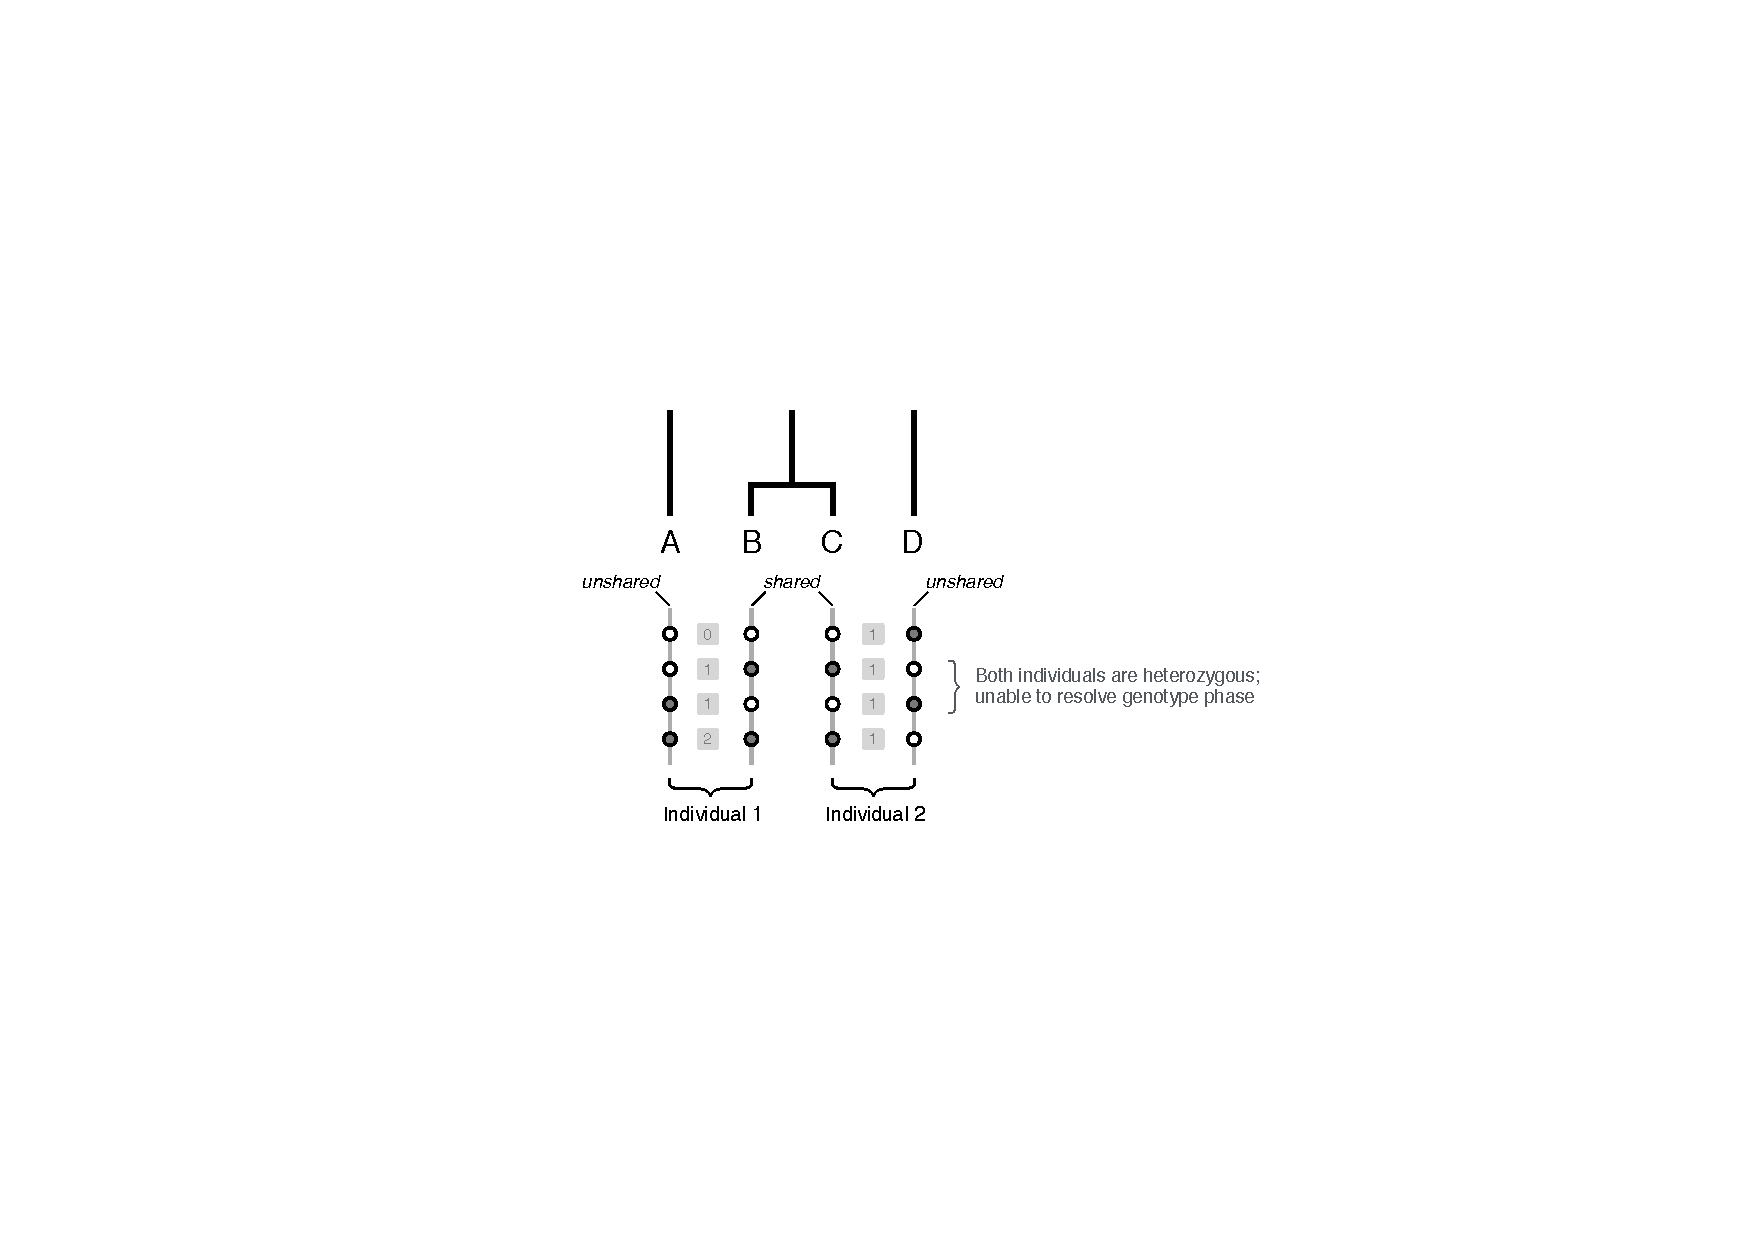
\includegraphics[width=0.75\textwidth]{./img/ch3/info_phase_pedigree}
\Caption{Genealogical constraints from haplotype sharing}
{The top graph indicates the genealogy of \n{4} haplotypes (A, B, C, and D) as seen in \n{2} individuals (1 and 2), which can be resolved partially if \n{2} haplotypes are shared by descent.
Below, the allelic states are shown at \n{4} positions along the sequence for each haplotype; ancestral and derived states are indicated by \emph{hollow} and \emph{solid} circles.
Only the genotypic state is seen in each individual as indicated between individual haplotypes; \ie homozygous for the ancestral allele (0), heterozygous (1), and homozygous for the derived allele (2).
The phase of a genotype can be resolved at sites with \n{1} homozygous genotype (phasing is redundant if both genotypes are homozygous).
Genotype phase cannot be determined if both individuals are heterozygous.}
{fig:info_phase_pedigree}
\end{figure}

% %
%
% A set of rules can be formulated which define the state of the shared allele if a certain genotype pair is observed in the \n{2} individuals considered.
% As before, the infinite sites model is assumed.
% If both genotypes are homozygous for the same allele, the deduction of the shared allele is trivial.
% If they are homozygous for different alleles, they cannot share an allele.
% Importantly, because this is seen at breakpoint sites detected using the \gls{dgt}, which mark the limits of the underlying IBD segment, breakpoints are excluded from this analysis; recall that the \gls{fgt} cannot be used with genotype data.
% A caveat of this analysis, however, is that haplotypes cannot be distinguished if both individuals are heterozygous, as it is not known whether the allele is shared or not.
% This conflict arises because an unshared haplotype may be more closely related to either the shared or the other unshared haplotype.
% Thus, haplotype inference is restricted to sites at which \emph{heterozygous-homozygous} genotype pairs are found.
% This is further illustrated in \cref{fig:info_phase_pedigree}.
%
% %
% % !TEX root = ../../main.tex


\begin{table}[!htb]
\Caption{Shared haplotype inference from genotype pairs}
{Given the \n{2} genotypes observed at a pair of individuals (A and B), there are \n{9} possible ordered combinations of alleles.
The corresponding haplotypes are shown for both individuals (unordered).
Note that genotype phase cannot be resolved for individuals that are both heterozygous; \ie the corresponding certainty score is equal to $\rfrac{1}{2}$.
If a pair is homozygous for different alleles, they do not share a haplotype.}
{tab:shared_hap_rules}
\centering
\begin{tabular}{ccccc}
\toprule
Genotype & Genotype &  Haplotypes & Haplotypes & Shared  \\
Individual $A$ & Individual $B$ &  Individual $A$ & Individual $B$ & haplotype  \\
\midrule
0  &  0  &  $(0,0)$  &  $(0,0)$  &  0  \\
0  &  1  &  $(0,0)$  &  $(0,1)$  &  0  \\
0  &  2  &  $(0,0)$  &  $(1,1)$  &  -- \\
1  &  0  &  $(0,1)$  &  $(0,0)$  &  0  \\
1  &  1  &  $(0,1)$  &  $(0,1)$  &  -- \\
1  &  2  &  $(0,1)$  &  $(1,1)$  &  1  \\
2  &  0  &  $(1,1)$  &  $(0,0)$  &  -- \\
2  &  1  &  $(1,1)$  &  $(0,1)$  &  1  \\
2  &  2  &  $(1,1)$  &  $(1,1)$  &  1  \\
\bottomrule
\end{tabular}
\end{table}

% %
%
% A complete definition of these rules is given in \cref{tab:shared_hap_rules}.
% The table gives the inferred allelic state of the shared haplotype for each of the possible combinations of \n{2} genotypes.
% Note that the alleles at \emph{heterozygous-heterozygous} sites are likely to be shared if \n{3} conditions are met; first, if the allele frequency at that site is lower than the frequency at the target position, second, if the allele only segregates within the subsample sharing the focal allele and, third, if the genealogy does not change along the sequence within an inferred interval.
% An allele that is lower in frequency is likely to be younger than the focal allele and, thus, to \Correct{be shared by some of the haplotypes within the sub-tree of the focal mutation}.
% However, this may only be the case under the infinite sites model, \eg because recurrent or back mutation may otherwise suggest a different genealogical order of descent.
%



%
\section{Evaluation}
%

The IBD detection method presented in this chapter was evaluated using simulated data.
This allowed assessment of the accuracy of detected breakpoint intervals in relation to the known genealogy of the simulated sample.
For comparison, an alternate IBD detection method was applied to the same data.
Lastly, the method presented was applied to data from the \glsentrylong{1kg}.



%
\subsection{Data generation}
\label{sec:msprime}
%

The coalescent simulator used to generate data was \texttt{msprime} (version~{0.4.0}), which simulates the exact coalescent with recombination, and where mutations are generated under the infinite sites model \citep{Kelleher:2016fn}.\footnote{Coalescent simulator \texttt{msprime}: \url{https://github.com/jeromekelleher/msprime} \accessed{2016}{11}{12}}
The software is a reimplementation of the classic \texttt{ms} algorithm by \citet{Hudson:2002vy}, but allows efficient simulation of extended chromosomal regions for very large sample sizes, where the entire history of the simulated sample can be stored and queried for further analysis.
Notably, \texttt{msprime} allows simulation under variable recombination rates, for example by using established recombination maps of the human genome.


%
\subsubsection{Demographic model}
\label{sec:sim_demo_model}
%

A demographic model was defined following \citet{Gutenkunst:2009gs}, who used intergenic data from \n{4} global populations to estimate parameters from diffusion approximations of expected allele frequency spectra.
Accordingly, here, data were simulated with an ancestral population size of ${\Ne = \num{7300}}$ (denoted by $N_A$ in the model) and under the assumption of a generation time of 25 years.
The mutation rate was set to a constant ${\mu = \num[round-precision=2]{2.35e-8}}$ per site per generation, which was estimated from the human-chimp divergence in \citet{Gutenkunst:2009gs}.
Note that recent studies have estimated the human mutation rate to be slightly lower; for example, \citet{Scally:2012fe} have estimated ${\mu \approx \num[round-precision=1]{1.2e-8}}$ from analyses of genome-wide \emph{de~novo} mutations using recent sequencing technologies.
\Correct{The mutation rate used here is two-fold higher, but still in the same order.}

%
%!TEX root = ../../main.tex


\begin{figure}[!htb]
\centering
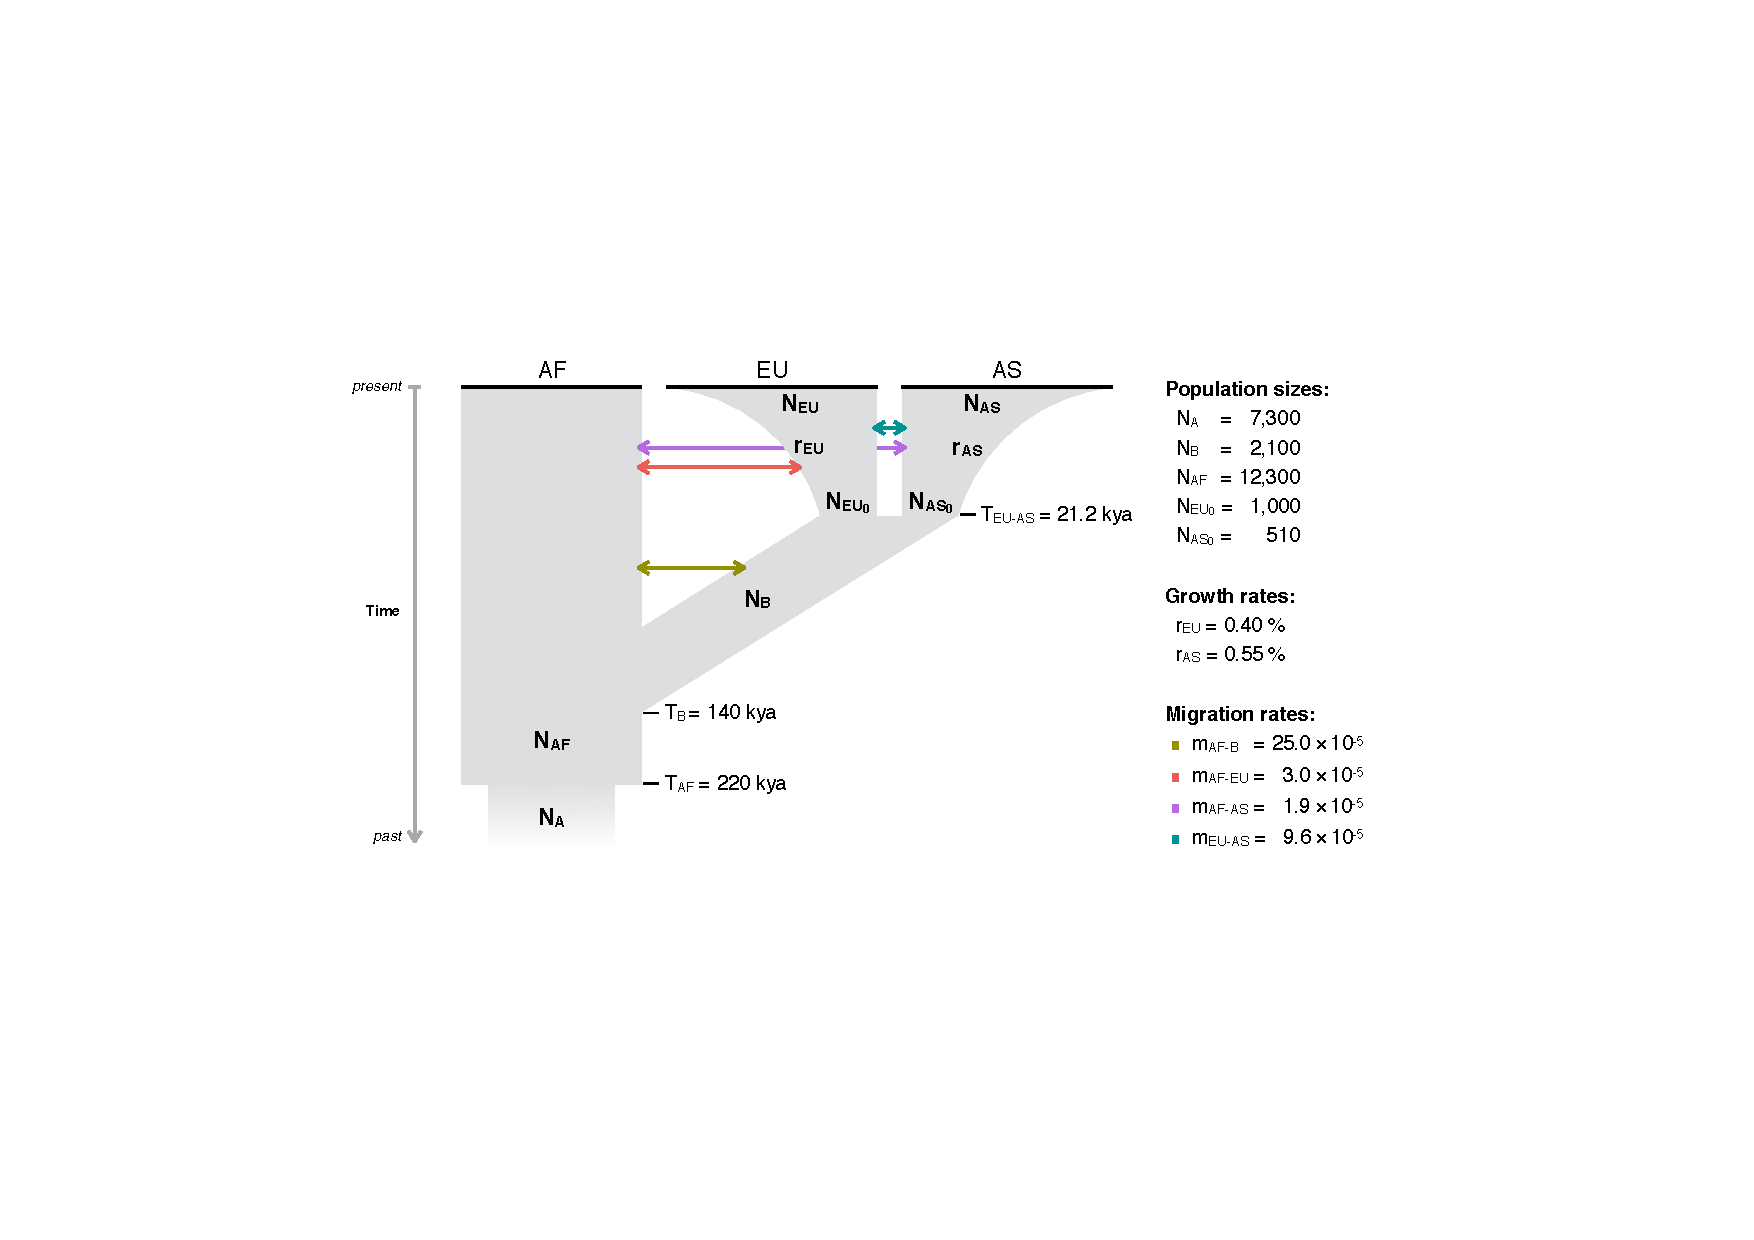
\includegraphics[width=0.95\textwidth]{./img/ch3/demo_model}
\Caption{Demographic model used in simulations}
{\N{3} populations were modelled, African (AF), European (EU), and Asian (AS), which derive from an ancestral population (A).
Both EU and AS experienced a bottleneck with subsequent exponential growth following the out-of-Africa expansion of a founder population (B) that split from the ancestral population.
Modified from \citet{Gutenkunst:2009gs}, Figure~2 (see \url{doi:10.1371/journal.pgen.1000695.g002}), with parameter values taken from Table~1 (see \url{doi:10.1371/journal.pgen.1000695.t001}).}
{fig:demo_model}
% \vspace{-5pt}
% \hrulefill%
\end{figure}

%

The demographic history as defined in the simulation model is illustrated in \cpref{fig:demo_model}; parameter values of the model are specified therein.
The model recapitulates the human expansion out of Africa, for which \n{3} populations were considered; African (AF), European (EU), and Asian (AS).
The African population was included with a constant population size, while EU and AS experienced exponential growth after divergence and split from an ancestral African population.
Population sizes of EU and AS were calculated as ${N = \rfrac{N_0}{\euler{-r t}}}$, where $N$ is the size at present, $N_0$ the initial size at EU-AS divergence, $r$ the growth rate, and $t$ the time since divergence (in years).


%
\subsubsection{Simulated dataset}
%

A sample of \n{5000} haplotypes was simulated, where the set of generated chromosomes represented a sample taken from the EU population.
To reproduce realistic distributions of recombination variability along the simulated sequence, the simulation was performed using recombination rates from human chromosome~20, as provided in Build~37 of the \gls{hapmap} Phase~\rom{2} \citep{Frazer:2007kha, InternationalHapMapConsortium:2010en}.\footnote{HapMap recombination map: \url{ftp://ftp.ncbi.nlm.nih.gov//hapmap/recombination/2011-01_phaseII_B37/genetic_map_HapMapII_GRCh37.tar.gz} \accessed{2016}{11}{12}}
\Addition{Note that the ratio between genetic and physical length on human chromosome~20 is $\approx\SI[per-mode=fraction,round-precision=1]{1.7}{\centi\morgan\per\mega\basepair}$, which differs from the average observed for the human genome at $\approx\SI[per-mode=fraction,round-precision=1]{1.2}{\centi\morgan\per\mega\basepair}$.}
The resulting dataset consisted of \dec{0.672847}~million segregating sites observed over a chromosomal length of \SI{62.949301}{\mega\basepair} (\SI{108.26675653}{\centi\morgan}).
The history of the simulated sample was stored separately to derive genealogical information in subsequent analyses.

The simulated chromosomes were used to generate \n{3} datasets.
In the first, haplotypes were randomly paired to construct a sample of \n{2500} diploid individuals.
From this, second, a corresponding genotype dataset was generated by forming genotypes (encoded as 0, 1, and 2) as the sum of alleles (encoded as 0 and 1) along the sequence in each individual.
This dataset was then used to generate a third dataset in which haplotypes were estimated from genotype data;
\ie resulting data consisted of phased haplotypes.
Phasing was conducted using \texttt{SHAPEIT} version~2 \citep{Delaneau:2008dk,Delaneau:2013hi}, using default parameters without a reference panel.\footnote{Phasing software \texttt{SHAPEIT}: \url{https://mathgen.stats.ox.ac.uk/genetics_software/shapeit/shapeit.html} \accessed{2016}{11}{12}}


%
\subsection{Accuracy analysis}
\label{sec:ibd_analysis}
%

The detection of IBD was evaluated in relation to the underlying true IBD structure of the sample, which was determined from the stored simulation records.
Given a target site and the \n{2} haplotypes sharing the focal allele, the genealogy was scanned along the sequence of variant sites observed in the sample, in both directions from the target position.
The \gls{mrca} of the pair was identified at each variant site and a breakpoint was defined as the first site at which a different \gls{mrca} was found.
This returned the smallest interval detectable from available data around the nearest recombination events that delimit an IBD segment.

Accuracy was measured in terms of the \Correct{physical} distance between a given breakpoint site and the focal position of the segment.
\N{2} measurements were considered; the squared Pearson correlation coefficient, $r^2$, which measures the strength of the linear relation between detected and true distance, and the \gls{rmsle};
\begin{equation}\label{eq:rmsle}
	\rmsle = \sqrt{ \frac{1}{n} \sum_{i=1}^n \Big[\log_{10}\Big(\frac{\hat{d}_i + 1}{d_i + 1}\Big)\Big]^2 }
\end{equation}
where $d_i$ and $\hat{d}_i$ are the distances of the true and detected breakpoints, respectively, and $n$ is the overall number of comparisons.
The \gls{rmsle} is similar to the root mean squared error (RMSE), which measures the variance and bias in the set of compared values, and is equal to the standard deviation when there is no bias.
As such, the \gls{rmsle} can be interpreted as a score metric for the magnitude of error.
Here, this is useful because larger departures from the actual values are penalised more than smaller ones.
A lower score value indicates a lower magnitude of error, where ${\rmsle = 0}$ indicates that true and inferred values are identical.
Also, note that the \gls{rmsle} is usually defined using the natural logarithm; here, $\log_{10}$ was used as a more intuitive representation of error magnitude.



The performance of the proposed IBD detection method was assessed for the described haplotype and genotype-based tests on the \n{3} datasets derived from coalescent simulations.
The following approaches were distinguished:
\begin{approach}\setlength\itemsep{0em}
\item\label{app:fgt_h} \gls{fgt} on haplotype data as simulated; \ie \emph{true} haplotypes,
\item\label{app:fgt_p} \gls{fgt} on \emph{phased} haplotypes, and
\item\label{app:dgt} \gls{dgt} on genotype data.
\end{approach}


%
\section{Results}
\label{sec:ibd_results}
%

IBD detection was carried out on a large set of target sites, for which all \fk{} variants found at ${k \in \lbrace 2, \ldots, 25 \rbrace}$ were selected, \ie alleles shared at frequency ${\leq 0.5\%}$.
This threshold was chosen arbitrarily, but such that the considered frequency range was expected to be sufficiently low to identify recent IBD given the size of the sample.
The set of target sites comprised \dec{0.317020}~million \glspl{snp} that were heterozygous in the individuals sharing a focal allele.
This resulted in \dec{11.597968}~million pairwise analyses and an equal number of IBD segments detected using the \gls{fgt} on the true and phased haplotypes in \cref{app:fgt_h,,app:fgt_p}, respectively, and the \gls{dgt} on genotype data in \cref{app:dgt}.

Because the same IBD interval may be inferred from multiple shared alleles in a given haplotype pair, the analysis was reduced to the set of uniquely detected segments per pair in each approach.
Duplicate segments were removed by sorting identical intervals by the frequency of target alleles, where only the segment detected around the allele of the lowest frequency was retained (and sampled if multiple shared alleles occurred at the same frequency).
Detected segments were thereby tagged by the presumably youngest shared allele within a given interval.
\Correct{This enabled the analysis to measure breakpoint accuracy conditional on the frequency of the target allele, which otherwise may have produced biased results due to sharing of higher-frequency alleles that are presumed to be older than the \gls{tmrca} of the underlying shared haplotype.}

The number of uniquely identified segments differed slightly in \cref{app:fgt_h,,app:fgt_p,,app:dgt};
\dec{2.983342}~million (\SI{25.72297}{\percent}),
\dec{3.091288}~million (\SI{26.65370}{\percent}), and
\dec{2.978238}~million (\SI{25.67896}{\percent}), respectively.
For the corresponding true IBD segments, the number of unique segments was \dec{3.001053}~million (\SI{25.87568}{\percent}).
These data were further reduced to the intersection of retained target sites across approaches, so as to enable direct comparisons on the same set of targets, which resulted in \dec{2.978220}~million (\SI{25.67881}{\percent}) unique intervals.
The results obtained from these data are summarised in \cpref{tab:stat_breakpoints}.

%
% !TEX root = ../../main.tex


\begin{table}[!htb]
\Caption{Accuracy of detected breakpoints per $\textbf{f}_{k}$~category}
{The accuracy of detected IBD breakpoints was measured using the squared Pearson correlation coefficient, $r^2$, and the \gls{rmsle} in relation to the true IBD segments determined from simulation records; measured in terms of the distance between breakpoint site and the corresponding focal position per segment.
The analysis included of \n{317020} target sites around which IBD was detected in \cref{app:fgt_h,,app:fgt_p,,app:dgt}.
In each, accuracy was computed after data were reduced to identical sets of unique IBD segments (${n=\num{2978220}}$).
The table specifies the allele frequency~(\%) corresponding to each \fk{}~category, as well as the number of target sites identified.}
{tab:stat_breakpoints}
\centering
\begin{threeparttable}
\begin{tabular}{
cc
S[table-format=6.1]
*3{S[table-format=1.3]}
c
*3{S[table-format=1.3]}}
\toprule
\fk{} & Freq.~{\%} & \multicolumn{1}{c}{Targets} &
\multicolumn{3}{c}{$r^2$} & &
\multicolumn{3}{c}{$\rmsle$} \\
\cmidrule(lr){4-6}
\cmidrule(lr){8-10}
 & & &
 \multicolumn{1}{c}{\textsc{fgt}$^{\ast}$} &
 \multicolumn{1}{c}{\textsc{fgt}$^{\ast\ast}$} &
 \multicolumn{1}{c}{\textsc{dgt}$^{\dagger}$} & &
 \multicolumn{1}{c}{\textsc{fgt}$^{\ast}$} &
 \multicolumn{1}{c}{\textsc{fgt}$^{\ast\ast}$} &
 \multicolumn{1}{c}{\textsc{dgt}$^{\dagger}$} \\
\midrule
2  & 0.04 & 76515  &  \bfseries 0.99764 & 0.89458 & 0.99520  & &  \bfseries 0.21948 & 0.59833 & 0.31710 \\
3  & 0.06 & 46138  &  \bfseries 0.98869 & 0.95705 & 0.97784  & &  \bfseries 0.24316 & 0.51595 & 0.35887 \\
4  & 0.08 & 31658  &  \bfseries 0.96294 & 0.95872 & 0.94097  & &  \bfseries 0.25555 & 0.46282 & 0.37881 \\
5  & 0.10 & 23581  &  \bfseries 0.97480 & 0.96275 & 0.92906  & &  \bfseries 0.27554 & 0.42873 & 0.40830 \\
6  & 0.12 & 19241  &  \bfseries 0.95448 & 0.93766 & 0.90396  & &  \bfseries 0.28086 & 0.40886 & 0.42082 \\
7  & 0.14 & 15869  &  \bfseries 0.95501 & 0.94390 & 0.89159  & &  \bfseries 0.29827 & 0.40264 & 0.44651 \\
8  & 0.16 & 13175  &  0.89794 & \bfseries 0.91758 & 0.81310  & &  \bfseries 0.31984 & 0.39805 & 0.46935 \\
9  & 0.18 & 10966  &  \bfseries 0.93158 & 0.92740 & 0.82685  & &  \bfseries 0.31402 & 0.37511 & 0.46718 \\
10 & 0.20 & 11142  &  0.87942 & \bfseries 0.88681 & 0.77257  & &  \bfseries 0.33200 & 0.38713 & 0.49355 \\
11 & 0.22 &  9392  &  \bfseries 0.89481 & 0.89213 & 0.75844  & &  \bfseries 0.34414 & 0.40133 & 0.51339 \\
12 & 0.24 &  7751  &  0.83526 & \bfseries 0.84776 & 0.73282  & &  \bfseries 0.35792 & 0.39763 & 0.52569 \\
13 & 0.26 &  6933  &  \bfseries 0.84208 & 0.83534 & 0.72078  & &  \bfseries 0.36065 & 0.40463 & 0.53176 \\
14 & 0.28 &  5767  &  \bfseries 0.81623 & 0.81622 & 0.67937  & &  \bfseries 0.36694 & 0.39075 & 0.54006 \\
15 & 0.30 &  5062  &  \bfseries 0.87140 & 0.86023 & 0.71246  & &  \bfseries 0.38095 & 0.40601 & 0.55560 \\
16 & 0.32 &  4711  &  \bfseries 0.83929 & 0.82998 & 0.70121  & &  \bfseries 0.37271 & 0.39465 & 0.54617 \\
17 & 0.34 &  4210  &  0.82865 & \bfseries 0.83173 & 0.68057  & &  \bfseries 0.38680 & 0.41049 & 0.56620 \\
18 & 0.36 &  3913  &  0.81267 & \bfseries 0.83171 & 0.67040  & &  \bfseries 0.37969 & 0.39699 & 0.56071 \\
19 & 0.38 &  3684  &  \bfseries 0.80141 & 0.79804 & 0.64162  & &  \bfseries 0.38074 & 0.40128 & 0.56564 \\
20 & 0.40 &  3214  &  0.83058 & \bfseries 0.83677 & 0.68478  & &  \bfseries 0.40090 & 0.41599 & 0.58737 \\
21 & 0.42 &  3333  &  0.77276 & \bfseries 0.77758 & 0.60320  & &  \bfseries 0.39881 & 0.41259 & 0.58359 \\
22 & 0.44 &  2863  &  0.75260 & \bfseries 0.79505 & 0.57059  & &  \bfseries 0.39876 & 0.40632 & 0.58646 \\
23 & 0.46 &  2595  &  0.73156 & \bfseries 0.74493 & 0.59629  & &  \bfseries 0.41417 & 0.42509 & 0.59901 \\
24 & 0.48 &  2653  &  \bfseries 0.78359 & 0.77969 & 0.58121  & &  \bfseries 0.39649 & 0.40641 & 0.58343 \\
25 & 0.50 &  2654  &  0.70052 & \bfseries 0.72997 & 0.56030  & &  \bfseries 0.39960 & 0.40764 & 0.58521 \\
\bottomrule
\end{tabular}
\begin{tablenotes}\footnotesize
	\item[$\ast$] ~ \cref{app:fgt_h}, using the \gls{fgt} with true haplotypes
	\item[$\ast\ast$] ~ \cref{app:fgt_p}, using the \gls{fgt} with phased haplotypes
	\item[$\dagger$] ~ \cref{app:dgt}, using the \gls{dgt} with genotype data
\end{tablenotes}
\end{threeparttable}
\end{table}

% 21803
% 36501
% 49533
% 59157
% 69271
% 89298
% 86317
% 98192
% 106765
% 118180
% 121107
% 123542
% 132232
% 139403
% 146324
% 150165
% 147554
% 149660
% 162293
% 176537
% 187870
% 195883
% 162501
% 94297

% 18795
% 34042
% 47338
% 59683
% 69487
% 81376
% 91580
% 98374
% 105827
% 116829
% 123145
% 127134
% 130059
% 145055
% 147945
% 151803
% 157849
% 160246
% 164855
% 183665
% 177742
% 181959
% 195948
% 207484

%

The proportion of breakpoints that were overestimated (in relation to the corresponding true IBD breakpoints) was noticeably high overall; using the \gls{fgt}, \SI{97.3903}{\percent} and \SI{95.66553}{\percent} were overestimated in \cref{app:fgt_h,,app:fgt_p}, respectively.
However, overestimation was highest when the \gls{dgt} was used (\SI{98.36191}{\percent}) in \cref{app:dgt}.
Conversely, the proportion of underestimated breakpoints was lowest in \ref{app:dgt}, \SI{1.543153}{\percent}, and highest when haplotypes were phased in \ref{app:fgt_p}, \SI{4.146739}{\percent}; in \ref{app:fgt_h}, \SI{2.41782}{\percent} of breakpoints were underestimated.
The proportion of detected breakpoints that coincided with the corresponding true breakpoints was \SI{0.19180}{\percent}, \SI{0.187729}{\percent}, and \SI{0.094939}{\percent} in \ref{app:fgt_h}, \ref{app:fgt_p}, and \ref{app:dgt}, respectively.

% Accuracy was measured in terms of the distance between breakpoint site and the corresponding focal position per detected and true IBD segments.
The highest overall accuracy was found for the \gls{fgt} on true haplotypes, followed by the analysis on phased haplotypes, which had ${r^2 = \dec{0.9262482}}$ and ${r^2 = \dec{0.8922048}}$ in \cref{app:fgt_h,,app:fgt_p}, respectively.
The accuracy achieved by the \gls{dgt} was lower, but still considerably high with ${r^2 = \dec{0.8474036}}$ in \cref{app:dgt}.
This was also reflected in the \Correct{measured} magnitude of error (\gls{rmsle}), which was \dec{0.39983}, \dec{0.43407}, and \dec{0.56940} in \ref{app:fgt_h}, \ref{app:fgt_p}, and \ref{app:dgt}, respectively.
The measurement of accuracy was further broken down by the allele frequency of target variants (\fk{}~category); results are shown in \cpref{tab:stat_breakpoints}.
Accuracy decreased towards higher allele frequency in each approach.
For example, for \fk{2}~variants, $r^2$ was \dec{0.998}, \Correct{\dec{0.895}}, and \dec{0.995} in \ref{app:fgt_h}, \ref{app:fgt_p}, and \ref{app:dgt}, respectively,
which was reduced for \fk{25}~variants where ${r^2 = \dec{0.701}}$ in~\ref{app:fgt_h} and ${r^2 = \dec{0.730}}$ in~\ref{app:fgt_p}, but where \ref{app:dgt} was seen to decrease more rapidly by comparison (${r^2 = \dec{0.560}}$).

Notably, when haplotype data were phased in \cref{app:fgt_p}, accuracy was highest at \fk{5}~variants (${r^2 = \dec{0.963}}$), indicating that accuracy was decreased at lower frequencies.
Similarly, \gls{rmsle} scores reflected the same general pattern, but where the magnitude of error in \ref{app:fgt_p} was at a maximum at \fk{2}~variants.
\Correct{One explanation is that relatively long haplotype regions are more likely to be affected by phasing errors, in particular switch errors, to which the \gls{fgt} but not the \gls{dgt} is susceptible.
Hence, because \fk{2} haplotypes are likely to be longer compared to haplotypes tagged by higher-frequency alleles (as a higher frequency is indicative for an older age), phasing errors are more likely to fall within longer shared haplotype regions and thereby may facilitate an underestimation of shared haplotype lengths.}

%
% !TEX root = ../../main.tex


\begin{figure}[!htbp]
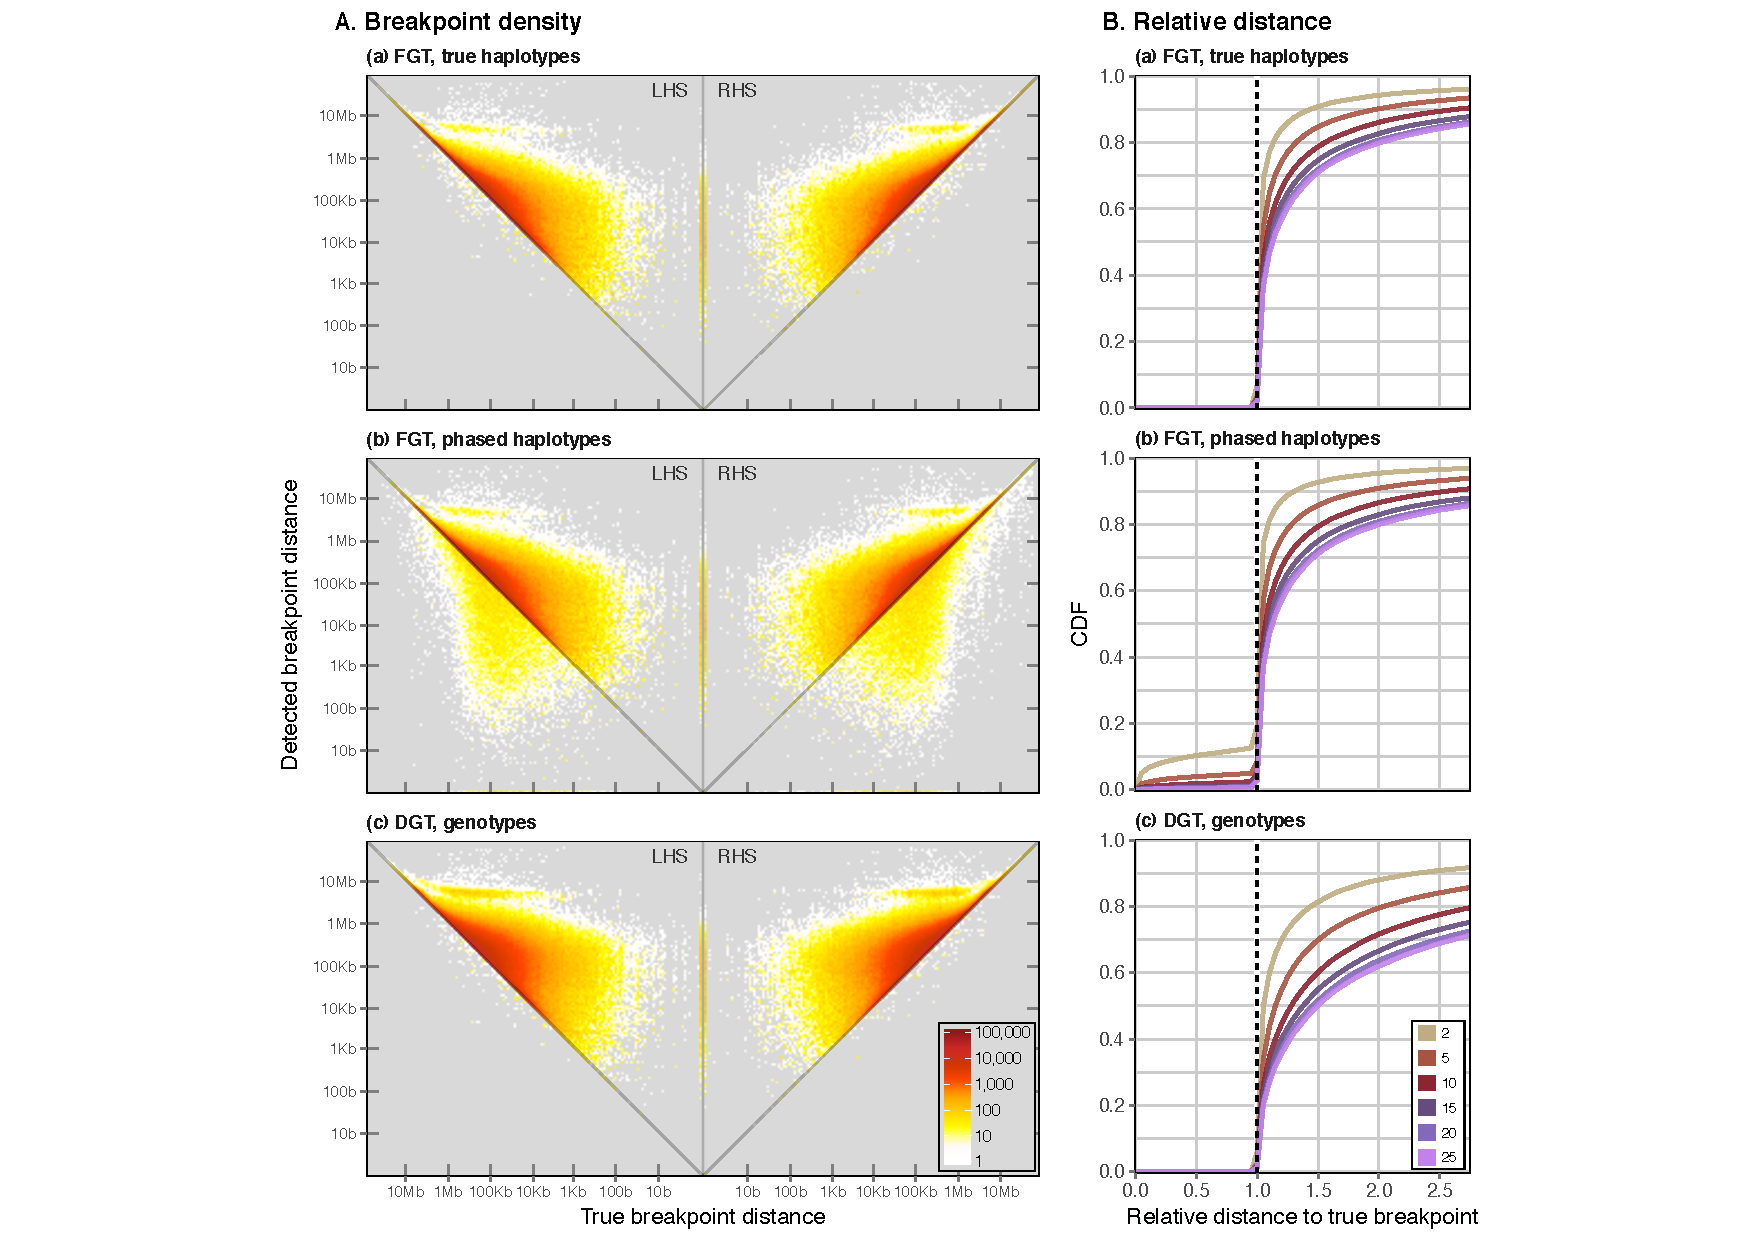
\includegraphics[width=\textwidth]{./img/ch3/naive_break_tru.pdf}
\Caption{Accuracy of breakpoint detection in simulated data}
{Breakpoints detected in \fk{} pairs at ${k \in \lbrace 2, \ldots, 25 \rbrace}$ are compared to true IBD breakpoint sites, after removing boundary cases in either the detected or true dataset.
Segments were inferred using the \gls{fgt} on true haplotypes \textbf{(a)} and phased haplotypes \textbf{(b)}, as well as the \gls{dgt} on genotype data \textbf{(c)}.
Panel~\textbf{(A)} illustrates the relationship between each detected breakpoint and the corresponding true breakpoint, measured as the physical distance to the focal site.
Along each axis, distances were pooled into \n{200} bins (on log scale)
and cells in the resulting $200^2$ grid were colour-coded for the number of  intersecting true and detected breakpoints, where grey indicates zero.
Segment breakpoints to the left (\emph{LHS}) and right-and side (\emph{RHS}) of the focal position are shown separately.
Panel~\textbf{(B)} shows the \gls{cdf} of detected breakpoints in relative distance to the focal and true breakpoint sites.
The physical distance between detected breakpoint and focal position was divided by the distance between true breakpoint and focal position, such that values $<1$ indicate underestimation and $>1$ overestimation relative to the true distance (\emph{dashed line}).}
{fig:naive_break_tru}
% \vspace{-5pt}
% \hrulefill
\end{figure}

%

A more intuitive representation of results is provided in \cpref{fig:naive_break_tru}, which compares true and detected breakpoint distances in \n{2} ways.
First, in \cref{fig:naive_break_tru}{A}, breakpoint densities are shown in separate scatterplots for breakpoints detected on the left and right-hand side of focal positions.
For example, a clear difference in the proportion of underestimated breakpoints can be seen between \cref{app:fgt_h,,app:fgt_p}, \ie where the \gls{fgt} was used on true and phased haplotypes, respectively.
In \cref{app:dgt}, where the \gls{dgt} was used on genotype data, breakpoint densities indicate a higher proportion of overestimated distances compared to \ref{app:fgt_h} or \ref{app:fgt_p}.
Second, in \cref{fig:naive_break_tru}{B}, the relative distance was calculated as ${x=\rfrac{\hat{d}_i}{d_i}}$, where $\hat{d}$ and $d$ denote detected and true distances, respectively.
By doing so, detected breakpoint distances were ``mapped'' relative to the corresponding true distances, such that ${0<x<1}$ indicates underestimation and ${x>1}$ indicates overestimation.
The \gls{cdf} of the relative distance is shown separately per \fk{}~category.
For example, it can be seen that a larger proportion of \fk{2}~variants (\SI{15.21486}{\percent}) contributed to the overall underestimation found in \cref{app:fgt_p}, \eg compared to \fk{5} (\SI{5.543963}{\percent}) and \fk{25}~variants (\SI{0.755359}{\percent}).


%
% !TEX root = ../../main.tex


\begin{figure}[!htb]
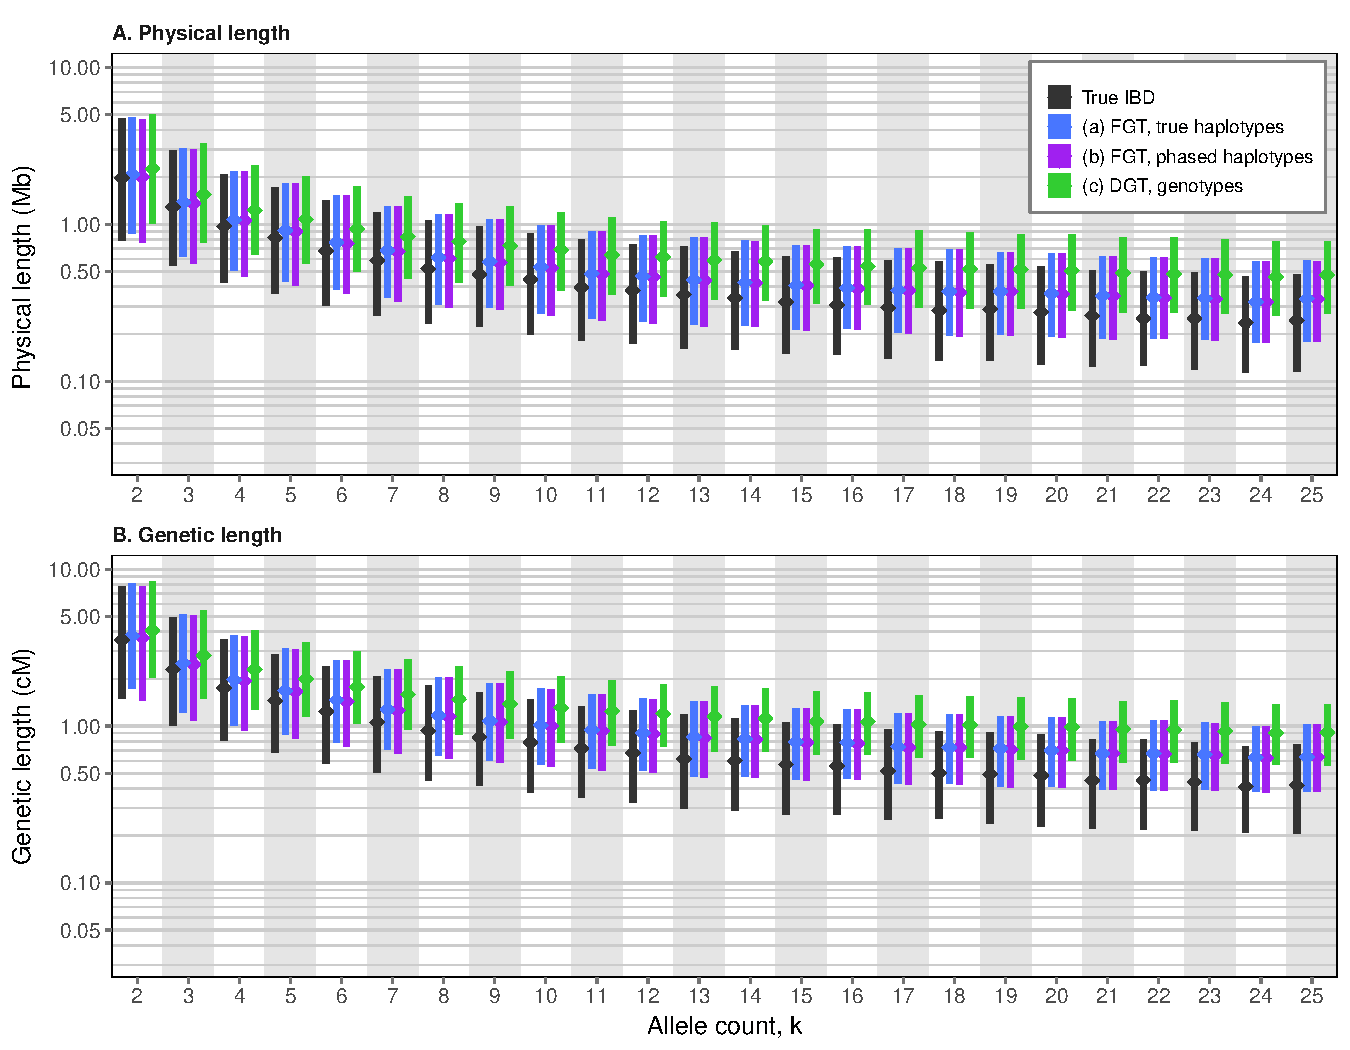
\includegraphics[width=\textwidth]{./img/ch3/naive_length_tru}
\Caption{IBD segment lengths inferred in simulated data}
{The distribution of median physical and genetic length of detected IBD segments is shown by allele frequency of the focal variant (\fk{[2,25]}).
IBD detection was performed using the \gls{fgt} on true and phased haplotypes, as well as the \gls{dgt} on genotype data; \cref{app:fgt_h,,app:fgt_p,,app:dgt}, respectively.
The true IBD length is shown for comparison.
Bottom and top of each bar indicate \nth{1} and \nth{3} quartiles, respectively, between which the median (\nth{2} quartile) is marked (\emph{diamonds}).}
{fig:naive_length_tru}
\end{figure}

%

The distribution of physical and genetic IBD length is shown in \cpref{fig:naive_length_tru}.
These results were obtained after boundary cases were removed in each approach (\ie discarding segments where the end of a chromosome was reached without detecting a breakpoint), so as to ensure that observed IBD length was delimited by recombination on both sides of a segment; \SI{1.448516}{\percent}, \SI{1.400165}{\percent}, and \SI{1.636716}{\percent}
were removed in \ref{app:fgt_h}, \ref{app:fgt_p}, and \ref{app:dgt}, respectively, and \SI{1.339693}{\percent} in the set of true IBD segments.
Data were then intersected again to retain the same set of target sites in each approach; as a result, \dec{2.929475}~million unique segments were retained (\SI{98.363284}{\percent}).

Median physical length (and median genetic length) over the set of retained segments was computed for each approach.
A small difference was seen for the \gls{fgt}, where median length was
\SI{0.4174283}{\mega\basepair} (\SI{0.8000373}{\centi\morgan})
on true haplotypes in \cref{app:fgt_h}, and
\SI{0.4126863}{\mega\basepair} (\SI{0.7905954}{\centi\morgan})
on phased haplotypes in \cref{app:fgt_p}.
For the \gls{dgt} on genotype data, median length was longer by comparison, \SI{0.5703613}{\mega\basepair} (\SI{1.0938442}{\centi\morgan}).
The median of true IBD length was \SI{0.3281641}{\mega\basepair} (\SI{1.5733807}{\centi\morgan}), which was shorter than detected in each approach.
But as seen in \cref{fig:naive_length_tru}, the distribution of IBD lengths in \ref{app:fgt_h}, \ref{app:fgt_p}, and \ref{app:dgt} closely followed the true lengths along the allele frequency range.
However, the gap between true and detected lengths increased towards higher allele frequencies.
For example, for \fk{2}~variants, median length of true IBD segments was
\SI{1.9775512}{\mega\basepair} (\SI{3.5510944}{\centi\morgan}),
which is only marginally shorter compared to
\SI{2.0786201}{\mega\basepair} (\SI{3.7725436}{\centi\morgan}),
\SI{2.0053149}{\mega\basepair} (\SI{3.6522954}{\centi\morgan}), and
\SI{2.2558099}{\mega\basepair} (\SI{4.0847501}{\centi\morgan})
in \ref{app:fgt_h}, \ref{app:fgt_p}, and \ref{app:dgt}, respectively.
For \fk{25}~variants the difference was more pronounced; \ie
median length of true IBD segments was
\SI{0.2433351}{\mega\basepair} (\SI{0.4194589}{\centi\morgan}),
compared to
\SI{0.3358179}{\mega\basepair} (\SI{0.6359137}{\centi\morgan}),
\SI{0.3345750}{\mega\basepair} (\SI{0.6338472}{\centi\morgan}), and
\SI{0.4750292}{\mega\basepair} (\SI{0.9073333}{\centi\morgan})
in \ref{app:fgt_h}, \ref{app:fgt_p}, and \ref{app:dgt}, respectively.


In summary, the \gls{fgt} on true haplotype data in \cref{app:fgt_h} overall achieved the highest levels of accuracy while maintaining low error.
This was particularly seen in comparison to \cref{app:fgt_p}, which differed only in the additionally included phasing step.
Since genomic datasets were typically composed of phased haplotypes, \cref{app:fgt_p} can be seen as being the realistic approach.
However, the higher error rate at lower frequency variants may pose a problem for analysis for rare variants.
As an alternative, the \gls{dgt} on genotype data, \cref{app:dgt}, can be used to detect IBD with high accuracy and comparatively low error rates.
However, the larger proportion of overestimated IBD breakpoints may result in additional error, \eg if it is assumed that the genealogy is consistent along the sequence of inferred IBD segments.




%
\subsubsection{IBD detection using the \emph{Refined\,IBD} algorithm}
\label{sec:ibd_beagle_tru}
%

\CorrectNote{Section rewritten to include corrections and additional results.}

Simulated data were additionally analysed using the \texttt{Refined\,IBD} algorithm implemented in \texttt{Beagle} version~4.1 \citep{Browning:2013eh}.\footnote{Beagle 4.1: \url{https://faculty.washington.edu/browning/beagle/beagle.html} \accessed{2016}{11}{22}}
The method is based on the non-probabilistic \texttt{GERMLINE} algorithm \citep{Gusev:2009hd}, which identifies putative IBD segments from short exact matches between haplotype pairs.
Candidate segments are then found by extending identified regions to longer inexact matches.
In \texttt{Refined\,IBD}, an additional probabilistic approach is included to assess candidate segments conditional on the \gls{lr} of the data, calculated under IBD and non-IBD models.
A \gls{lod} score is calculated as ${\log_{10}(\text{LR})}$, and segments are reported as IBD if the \gls{lod} score is above a specified threshold.
This approach has been found to achieve greater accuracy than \texttt{GERMLINE} alone or \texttt{fastIBD}, which is a non-probabilistic method that detects IBD based on haplotype frequency \citep{Browning:2011do,Browning:2013eh}.

The method requires haplotype data and cannot be executed with genotype information alone.
In the following, \cref{app:fgt_h} refers to the analysis conducted on true haplotypes and \cref{app:fgt_p} on phased haplotypes.
The analysis was performed using default parameters in \texttt{Refined\,IBD} (retaining candidate segments at ${\mbox{LOD}>3.0}$) and after conversion of simulated data into \gls{vcf}\footnote{Variant Call Format: \url{http://vcftools.sourceforge.net/VCF-poster.pdf} \accessed{2016}{11}{22}}.


The purpose of the following analysis was to evaluate whether \texttt{Refined\,IBD} could be used as a method to detect recombination breakpoints and thereby the length of the underlying shared haplotype.
This was done by reference to the set of true IBD segments that was determined from simulation records for the set of previously analysed target sites at all \fk{[2,25]} variants found in the data (allele frequency $\leq 0.5\%$).
However, note that the detection approach employed by \texttt{Refined\,IBD} reports all segments inferred for a given pair of haplotypes, such that detected and true intervals cannot be matched by direct reference to a particular target site.
Hence, for each pair of haplotypes present in both sets (detected and true), it was necessary to match segments based on their intervals.
As a consequence, it was not possible, for example, to make statements about IBD segments falsely identified by \texttt{Refined\,IBD}, as these would be among the segments removed in the matching process.

In \cref{app:fgt_h}, the analysis returned \dec{13.688781}~million IBD segments at \dec{6.910821}~million haplotype pairs.
A similar number was returned in \cref{app:fgt_p}, where \dec{13.647038}~million segments were found at \dec{6.855710}~million pairs.
The haplotype pairs at which IBD could be inferred differed between these results;
for example, \dec{4.377713}~million pairs were present in both datasets.
The set of available true IBD segments contained \dec{11.597968}~million intervals at \dec{2.638412}~million pairs.
The number of pairs matched between each detected set and the true set was \dec{2.332363}~million in \ref{app:fgt_h} and \dec{1.661487}~million in \ref{app:fgt_p}.

The lower number of matched pairs in \cref{app:fgt_p} was due to mismatched haplotypes resulting from the phasing process.
Note that it was straightforward to account for haplotype mismatches in the previous analysis, where the focal haplotype could be identified from a given target allele, but which was not possible in the present analysis.
It would be possible, for example, to match segments by pair of individuals (instead of haplotype pair) to avoid haplotype mismatches due to phasing.
This would introduce a bias when evaluating the accuracy of detected haplotype breakpoints due to possible overlaps of shared haplotypes within the same pair of individuals.
To circumvent this bias, such segments were randomly sampled per individual pair if an overlap was found in the set of results returned in the analysis on the phased dataset, so as to allow the identification of the correct true IBD segment based on matching pairs of individuals.
This removed \dec{0.144859}~million detected IBD segments (\Percent{1.061468}) in \cref{app:fgt_p}, but increased the number of segments that could be matched to the set of true segments (\dec{1.886876}~million pairs).

In the following, two analyses were performed.
First, the sets of detected IBD segments in \cref{app:fgt_h,app:fgt_p} were matched to the set of true segments based on interval overlap.
The proportion of overlap was measured relative to both the inferred and true segments, where segments were ignored if none of the inferred intervals overlapped with any of the true segments available for a given pair.
Second, to facilitate comparisons to the targeted IBD detection method evaluated in the previous section, where the accuracy of breakpoint detection was measured in relation to a given target site, inferred segments were matched to the set of true segments based on the inferred interval containing a given target site.


%
% !TEX root = ../../main.tex


\begin{figure}[!htb]
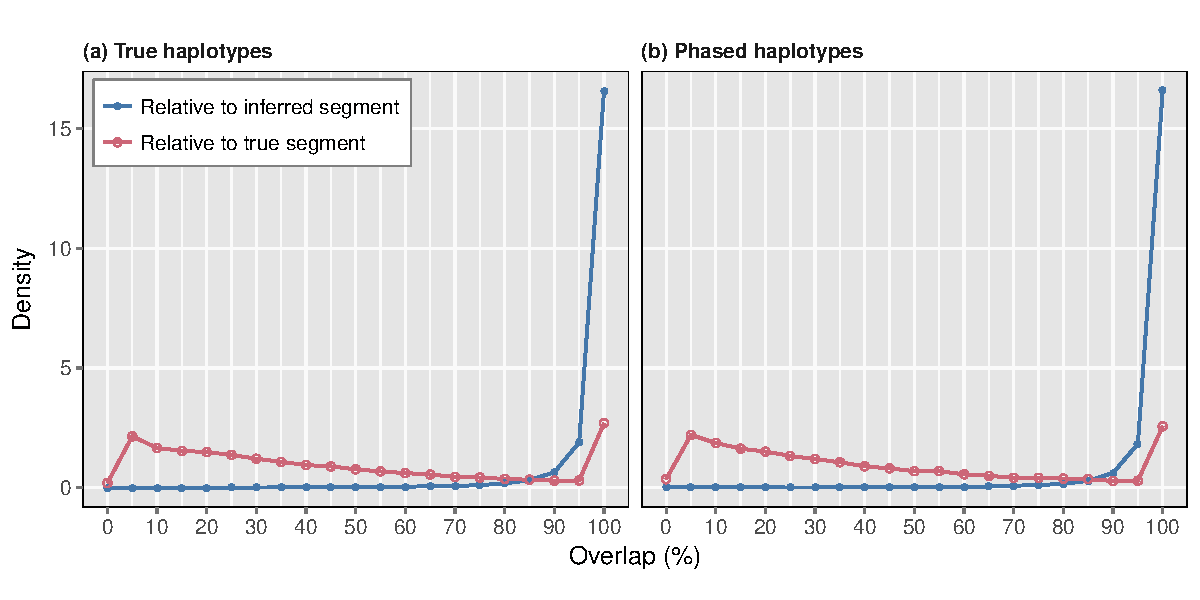
\includegraphics[width=\textwidth]{./img/ch3/beagle_overlap}
\Caption{IBD segment overlap inferred using \emph{Refined\,IBD} in Beagle~4.1}
{For a given pair, each of the inferred IBD segments were aligned with each of the true segments to determine the proportion of total base overlap; interval comparisons with zero overlap were ignored.
The reported densities refer to the proportion of overlap with respect to the inferred segment (\emph{blue}) and the true segment (\emph{red}).
\AdditionLabel}
{fig:beagle_overlap}
\end{figure}

%


When intervals were matched by overlap, on average, \Percent{97.8214} of an inferred interval overlapped with a true shared haplotype in \cref{app:fgt_h}, but only \Percent{42.97985} of a given true interval was covered by an inferred segment on average.
This was similar in \ref{app:fgt_p}; \Percent{97.39512} and \Percent{41.57889}, respectively.
The density of overlap measured relative to both the inferred and true segments is shown in \cpref{fig:beagle_overlap}.
These results indicate that the length of segments detected by \texttt{Refined\,IBD} were more likely to be underestimated, but where it is possible that the underlying shared haplotype may be covered by multiple, shorter segments.
For example, an average of \dec{1.137447} unique segments per pair was known from simulation records, but \dec{1.980775} and \dec{1.971152} segments were inferred per pair on average in \ref{app:fgt_h} and \ref{app:fgt_p}, respectively.



Next, the sets of inferred IBD segments returned in \cref{app:fgt_h,app:fgt_p} were matched to the set of true intervals by the condition that a given target site was contained in the inferred interval.
The matching process resulted in \dec{9.173353}~million segments in \ref{app:fgt_h}, but which were reduced to \dec{2.107930}~million by removing duplicate intervals per pair.
Likewise, \dec{8.958549}~million segments were matched in \ref{app:fgt_p}, which was reduced to \dec{2.083768}~million.

Recall that the set of true haplotypes contained all segments found around a given target site, but where multiple shared alleles may sit on the same shared haplotype.
To reduce such duplicates, identical intervals per pair were sorted by the frequency of target alleles, where only the segment around the shared allele with the lowest frequency was retained (and randomly sampled if multiple shared alleles occurred at the same frequency).
This enabled the analysis to measure breakpoint accuracy conditional on the frequency of the target allele.


%
% !TEX root = ../../main.tex


\begin{figure}[tb]
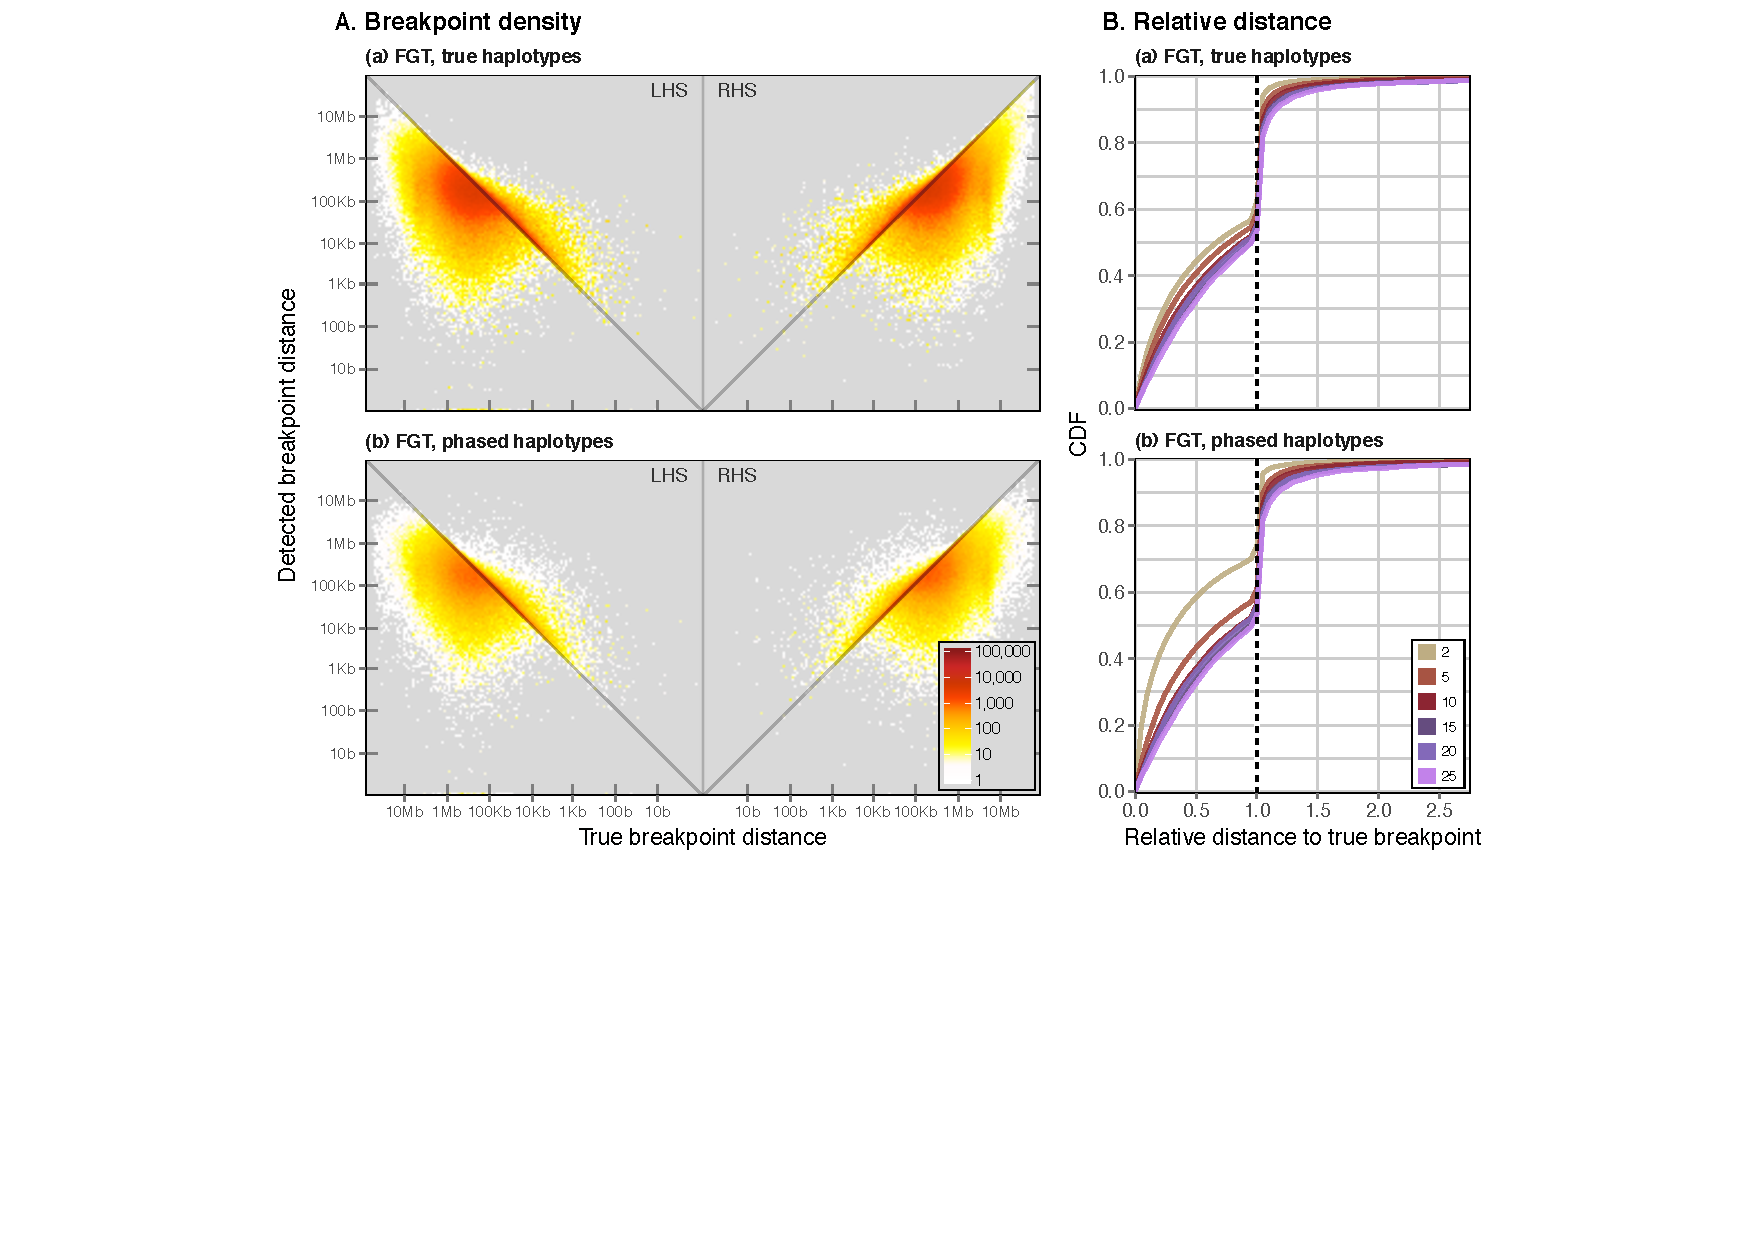
\includegraphics[width=\textwidth]{./img/ch3/beagle_break_tru}
\Caption{Accuracy of breakpoint detection in simulated data using Refined IBD in Beagle~4.1}
{Results are shown for uniquely detected shared haplotype segments inferred using the Refined IBD method; after removing boundary cases in either the detected or true segments, and after the detected segments were matched to the set of true segments.
Segments were inferred on true (simulated) haplotype data \textbf{(a)} and phased haplotypes \textbf{(b)}.
Panel~\textbf{(A)} provides a heatmap representation of a scatter plot, comparing physical distances between focal site and true breakpoint (x-axis) and detected breakpoint (y-axis).
Segment breakpoints to the left (\emph{LHS}) and right-and side (\emph{RHS}) of the focal position are shown separately.
Panel~\textbf{(B)} shows the \gls{cdf} of detected breakpoints in relative distance to the focal and true breakpoint sites.}
{fig:beagle_break_tru}
% \vspace{-5pt}
% \hrulefill%
\end{figure}

%


In reference to the matched true IBD intervals, \Percent{47.03292} and \Percent{45.9847} of the detected breakpoints were overestimated in \cref{app:fgt_h,app:fgt_p}, respectively,
while \Percent{49.8754} and \Percent{51.06569} were underestimated.
Differences due to phasing were seen at lower frequency target alleles, \eg at \fk{2}, for which
\Percent{48.35232} were underestimated in \ref{app:fgt_h} but \Percent{58.75466} \ref{app:fgt_p}.
The accuracy of breakpoint detection using \texttt{Refined\,IBD} is illustrated in \cpref{fig:beagle_break_tru}.


The density of true and detected breakpoints (\cref{fig:beagle_break_tru}{A}) suggests that the breakpoints inferred using \texttt{Refined\,IBD} were closely distributed around the corresponding true breakpoints.
However, overall accuracy was low in both \ref{app:fgt_h} and \ref{app:fgt_p}, reaching
${r^2 = \dec{0.3539768}}$ and
${r^2 = \dec{0.2092084}}$, respectively.
The magnitude of error, \gls{rmsle}, was similar in both \ref{app:fgt_h} \ref{app:fgt_p};
\dec{0.5339044} and
\dec{0.5477256}, respectively.
When true haplotypes were analysed, \cref{app:fgt_h}, accuracy decreased steadily towards higher allele frequencies.
For example, accuracy was highest for \fk{2}~variants
(${r^2 = \dec{0.52206694}}$) but lowest for \fk{25}~variants
(${r^2 = \dec{0.08020972}}$).
The magnitude of error was similar across allele frequencies, \eg at \fk{2}
(${\rmsle = \dec{0.5713065}}$) and \fk{25}~variants
(${\rmsle = \dec{0.5226131}}$).
When haplotypes were phased, \cref{app:fgt_p}, error was increased at \fk{2}~variants
(${\rmsle = \dec{0.7062560}}$) in comparison to \fk{25}~variants
(${\rmsle = \dec{0.5268743}}$).
The higher error at lower allele frequencies was also reflected in $r^2$~values; \eg accuracy was low at \fk{2}
(${r^2 = \dec{0.16387089}}$) and highest at \fk{3}
(${r^2 = \dec{0.21495542}}$), but lowest at \fk{25}
(${r^2 = \dec{0.07223534}}$).
The difference between true and phased datasets is further highlighted in  \cref{fig:beagle_break_tru}{B}, where a higher proportion of \fk{2}~variants is seen to be underestimated in \cref{app:fgt_p}.


%
% !TEX root = ../../main.tex


\begin{figure}[!htb]
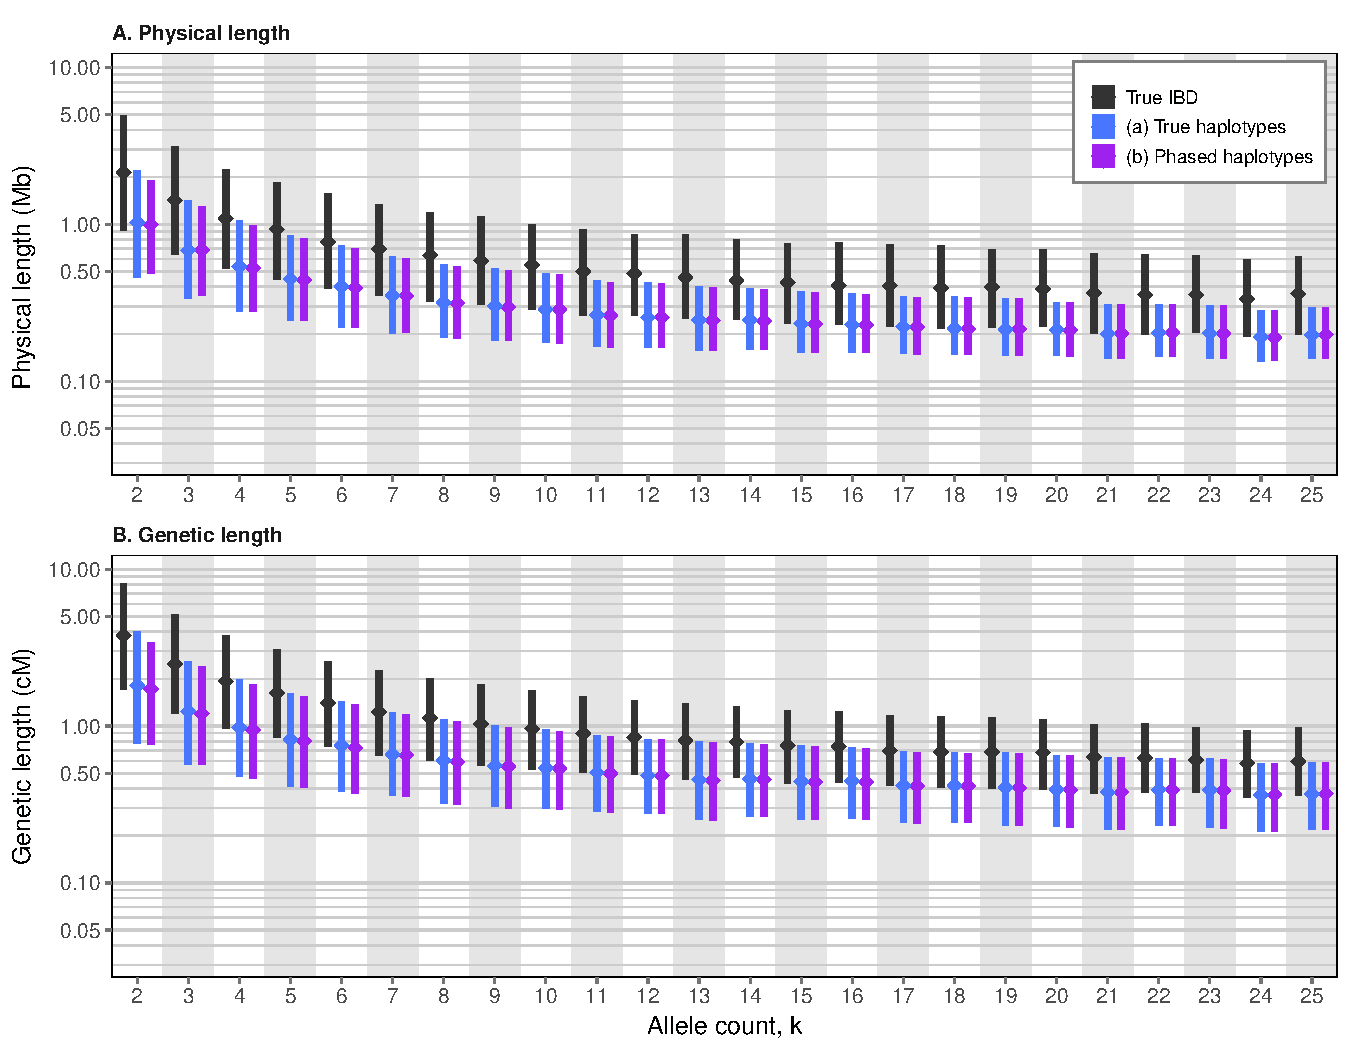
\includegraphics[width=\textwidth]{./img/ch3/beagle_length_tru_new}
\Caption{IBD segment lengths inferred using \emph{Refined\,IBD} in Beagle~4.1}
{The distribution of median physical \emph{(A)} and median genetic \emph{(B)} segment length is shown by allele count (\fk{}~category).
IBD segments were inferred using the \texttt{Refined\,IBD} algorithm implemented in \texttt{Beagle~4.1}, using true (simulated) haplotype data \ref{app:fgt_h} and phased haplotype data \ref{app:fgt_p}.
Bottom and top of each bar indicate \nth{1} and \nth{3} quartiles, respectively, between which the median (\nth{2} quartile) is marked (\emph{diamonds}).}
{fig:beagle_length_tru}
\end{figure}

%


The distribution of physical and genetic lengths for the segments retained in \cref{app:fgt_h,app:fgt_p} are in shown in \cpref{fig:beagle_length_tru}, in relation to the true IBD lengths at each \fk{}~category.
Because \ref{app:fgt_h} and \ref{app:fgt_p} were compared on different sets of detected segments, the reported lengths of true segments were computed from the set matched to \ref{app:fgt_h}.
Boundary cases were removed to avoid potential bias in length comparisons;
\Percent{1.682883} and
\Percent{1.665493} in \ref{app:fgt_h} and \ref{app:fgt_p}, respectively.

Overall median physical length (and median genetic length) was
\SI{0.239924}{\mega\basepair} (\SI{0.4575771}{\centi\morgan}) in \ref{app:fgt_h} and
\SI{0.238462}{\mega\basepair} (\SI{0.4533713}{\centi\morgan}) in \ref{app:fgt_p},
but both were shorter in comparison to the set of true IBD segments at
\SI{0.450181}{\mega\basepair} (\SI{0.7805489}{\centi\morgan}).
At \fk{2}~variants, the median length of IBD segments inferred in \ref{app:fgt_h} was
\SI{1.0257910}{\mega\basepair} (\SI{1.8123059}{\centi\morgan}),
which was longer compared to \ref{app:fgt_p}, where median length was
\SI{0.9945990}{\mega\basepair} (\SI{1.7275540}{\centi\morgan}).
However, both were considerably shorter in comparison to the true segments around \fk{2}~variants at
\SI{2.1377210}{\mega\basepair} (\SI{3.7699265}{\centi\morgan}).
This difference persisted towards higher allele frequencies; \eg for \fk{25}~variants;
\SI{0.1977400}{\mega\basepair} (\SI{0.3704905}{\centi\morgan}) in \ref{app:fgt_h} and
\SI{0.1974080}{\mega\basepair} (\SI{0.3699867}{\centi\morgan}) in \ref{app:fgt_p}, compared to the median length of the matched true segments at
\SI{0.3600640}{\mega\basepair} (\SI{0.5955694}{\centi\morgan}).


These results suggested that the lengths of inferred breakpoint intervals are likely to be shorter than the underlying haplotype region shared by descent.
Thus, the \texttt{Refined\,IBD} algorithm is less accurate with regard to the inference of the recombination breakpoints that delimit the underlying IBD tract.
It was not possible in this analysis to evaluate whether IBD was inferred incorrectly, as incorrect segments would have been removed in the matching process between the sets of inferred and true shared haplotype segments that were determined from simulation records.
However, by also evaluating the relative proportion of total base overlap between inferred and true intervals, it was indicated that IBD detection using \texttt{Refined\,IBD} is likely to result in multiple, shorter segments along the length of the underlying shared haplotype.


%
% NOTE: first version used wrong data somehow, and did not include the overlap analysis
%
% The accuracy of detected IBD segments was measured in relation to the true IBD intervals, which were already determined for the set of previously analysed target sites; \ie all \fk{[2,25]} variants found in the data (allele frequency $\leq 0.5\%$).
% The detection approach employed by \texttt{Refined\,IBD} reports all segments inferred for a given pair of haplotypes, such that detected and true intervals cannot be matched by direct reference to a particular target site.
% Hence, for a given pair of haplotypes, true and detected segments were matched if the focal allele associated with a true segment fell within the interval of the detected segment, which was discarded if none of the pairwise shared target alleles were found within the detected interval.
% This matching process resulted in a set of \dec{2.166492}~million unique segments in the analysis conduced on true haplotypes, \cref{app:fgt_h}.
% % This number is low when seen in relation to the full set of unique segments detected (\SI{0.1586614}{\percent}), but reasonably large in relation to the set of true unique segments available (\SI{72.19106}{\percent}).
% For the phased dataset, \cref{app:fgt_p}, \dec{0.528477}~million unique segments were matched.
% % , which corresponded to a lower proportion of retained segments in relation to both the full set (\SI{3.917097}{\percent}) and the set of true segments (\SI{17.76833}{\percent}).
% The lower number of segments retained in \cref{app:fgt_p} is likely to be the consequence of mismatched haplotypes in original and phased data.
%
%
% After the removal of segments at which haplotype pairs did not share any of the alleles in \fk{[2,25]}, median lengths were longer in comparison to the original datasets; \SI{0.255496}{\mega\basepair} and \SI{0.256070}{\mega\basepair} in \ref{app:fgt_h} and \ref{app:fgt_p}, respectively.
% This can be seen as the result of both the removal of falsely identified segments, as well as segments that were older and thereby expected to be shorter.
%
%
% The majority of retained breakpoints was underestimated in both \cref{app:fgt_h,,app:fgt_p}; \SI{55.35559}{\percent} and \SI{56.60644}{\percent}, respectively.
% In \cref{app:fgt_h}, \SI{44.38505}{\percent} were overestimated and \SI{0.2593594}{\percent} coincided with true breakpoint positions.
% This was similar in \cref{app:fgt_p}, where \SI{43.15511}{\percent} were overestimated and \SI{0.2384493}{\percent} coincided.
% Accuracy was measured in terms of the physical distance between breakpoint position and the corresponding focal site.
% Because the latter was not specified in the results obtained from \texttt{Refined\,IBD}, the same focal position as associated with the matched true IBD segment was assumed.
% Data were not reduced to the intersection of segments retained across datasets, due to the low number of consistent matches.
% These results are illustrated in \cpref{fig:beagle_break_tru}.
%
%
% The distance distribution of true and detected breakpoints (\cref{fig:beagle_break_tru}{A}) suggests that detected breakpoints were closely distributed around the corresponding true breakpoints.
% However, overall accuracy was low in both \ref{app:fgt_h} and \ref{app:fgt_p}, reaching ${r^2 = \dec{0.2868218}}$ and ${r^2 = \dec{0.1707155}}$, respectively.
% The magnitude of error, \gls{rmsle}, was lower in \ref{app:fgt_h} compared to \ref{app:fgt_p}; \dec{0.5954253} and \dec{0.6158843}, respectively.
% When true haplotypes were analysed, \cref{app:fgt_h}, accuracy decreased steadily towards higher allele frequencies.
% For example, accuracy was highest for \fk{2}~variants (${r^2 = \dec{0.34591189}}$) but lowest for \fk{25}~variants (${r^2 = \dec{0.07445725}}$).
% However, the magnitude of error was highest for \fk{2}~variants (${\rmsle = \dec{0.7498976}}$) and lowest for \fk{25}~variants (${\rmsle = \dec{0.5433645}}$).
% When haplotypes were phased, \cref{app:fgt_p}, error was further increased at \fk{2}~variants (${\rmsle = \dec{0.999}}$) in comparison to \fk{25}~variants (${\rmsle = \dec{0.5456303}}$).
% The higher error at lower allele frequencies was also reflected in $r^2$~values; \eg accuracy was low at \fk{2} (${r^2 = \dec{0.08720971}}$), higher at \fk{5} (${r^2 = \dec{0.13222751}}$), but lowest at \fk{25} (${r^2 = \dec{0.04827430}}$).
% The difference between true and phased datasets is further highlighted in  \cref{fig:beagle_break_tru}{B}, where a higher proportion of \fk{2}~variants is seen to be underestimated in \ref{app:fgt_p}.
%
%
% The distribution of physical and genetic lengths for the segments retained in \cref{app:fgt_h,,app:fgt_p} are in shown in \cpref{fig:beagle_length_tru}, in relation to the true IBD lengths at each \fk{}~category.
% Because \ref{app:fgt_h} and \ref{app:fgt_p} were compared on different sets of detected segments, the reported lengths of true segments were computed from the set matched to \ref{app:fgt_h}.
% Boundary cases were removed to avoid potential bias in length comparisons; \SI{1.012328}{\percent} and \SI{0.8926612}{\percent} in \ref{app:fgt_h} and \ref{app:fgt_p}, respectively.
%
%
% Overall median physical length (and median genetic length) was
% \SI{0.1851263}{\mega\basepair} (\SI{0.6206617}{\centi\morgan}) in \ref{app:fgt_h} and
% \SI{0.1915816}{\mega\basepair} (\SI{0.4289705}{\centi\morgan}) in \ref{app:fgt_p}, but both were shorter in comparison to true IBD segments at \SI{0.2600899}{\mega\basepair} (\SI{0.9115976}{\centi\morgan}).
% At \fk{2}~variants, the median length of IBD segments inferred in \ref{app:fgt_h} was \SI{1.1504220}{\mega\basepair} (\SI{1.8253656}{\centi\morgan}), which was longer compared to \ref{app:fgt_p}, where median length was \SI{1.1260528}{\mega\basepair} (\SI{1.7774934}{\centi\morgan}).
% However, both were considerably shorter in comparison to the true segments, \SI{3.4129234}{\mega\basepair} (\SI{5.2287476}{\centi\morgan}).
% This difference persisted towards higher allele frequencies; \eg for \fk{25}~variants, where the median of true lengths was
% \SI{0.3826137}{\mega\basepair} (\SI{0.6360041}{\centi\morgan}), which was
% longer compared to \SI{0.2015983}{\mega\basepair} (\SI{0.3778032}{\centi\morgan}) in \ref{app:fgt_h} and \SI{0.2018875}{\mega\basepair} (\SI{0.3730844}{\centi\morgan}) in \ref{app:fgt_p}.
%





%
\subsubsection{IBD detection in real data: 1000 Genomes, chromosome 20}
%

The IBD detection \Correct{methodology developed in this chapter (\gls{fgt} and \gls{dgt})} was applied to the final release dataset of the \glsentrylong{1kg} Phase~\rom{3} \citep{GenomesProjectConsortium:2012co,Auton:2015gk}, which included ${N=\num{2504}}$ individuals.
IBD detection was performed for each autosome (chromosomes 1--22), where selected target sites comprised all shared rare variants at allele frequency ${\leq 0.5\%}$; \ie \fk{} where ${k \in \{2, \ldots, 25\}}$.
However, to enable a closer comparison to the results obtained on the simulated dataset (which simulated variable recombination rates as inferred for chromosome~20), the following results are presented for chromosome~20 only.
A summary of the IBD detection results for chromosomes 1--22 is given in \cpref{tab:stat_ibd_1kg}.

%
% !TEX root = ../../main.tex


\begin{table}[!htbp]
\Caption{Inferred IBD length per chromosome in 1000 Genomes}
{Shared haplotype segments in \gls{1kg} Phase~\rom{3} were inferred using the \gls{fgt} and \gls{dgt}, on data from \n{2504} individuals across all autosomes.
Pairwise shared segments were identified from rare variants at allele frequency $\leq 0.5\%$ (\fk{[2,25]}).
Median genetic and physical lengths over all inferred segments were calculated per chromosome, after removing boundary cases and retaining unique segments only.}
{tab:stat_ibd_1kg}
\centering
\begin{threeparttable}
\begin{tabular}{%
c%
*2{S[table-format=7.0]}%
*1{S[table-format=8.0]}%
*2{S[table-format=2.1,round-precision=1]}%
*2{S[table-format=1.3]}%
*2{S[table-format=1.3]}%
}
\toprule
\multicolumn{1}{c}{Chr.} &
\multicolumn{1}{c}{SNPs} &
\multicolumn{1}{c}{Targets} &
\multicolumn{1}{c}{Segments} &
\multicolumn{2}{c}{Unique (\%)} &
\multicolumn{2}{c}{Length (Mb)} &
\multicolumn{2}{c}{Length (cM)} \\
\cmidrule(lr){5-6}
\cmidrule(lr){7-8}
\cmidrule(lr){9-10}
 & & & &
\multicolumn{1}{c}{\textsc{fgt}$^{\ast}$} &
\multicolumn{1}{c}{\textsc{dgt}$^{\ast\ast}$} &
\multicolumn{1}{c}{\textsc{fgt}$^{\ast}$} &
\multicolumn{1}{c}{\textsc{dgt}$^{\ast\ast}$} &
\multicolumn{1}{c}{\textsc{fgt}$^{\ast}$} &
\multicolumn{1}{c}{\textsc{dgt}$^{\ast\ast}$} \\
\midrule
 1 & 6196151 & 2126720 & 64449399 & 40.280460 & 35.860396 & 0.12450800 & 0.23689200 & 0.15004290 & 0.29955537 \\
 2 & 6786300 & 2323889 & 70274554 & 38.120313 & 33.836819 & 0.13578100 & 0.24753300 & 0.14312010 & 0.28022980 \\
 3 & 5584397 & 1893872 & 57220884 & 37.133805 & 33.195049 & 0.13777500 & 0.24292100 & 0.15395287 & 0.29019708 \\
 4 & 5480936 & 1847521 & 57598118 & 36.609335 & 32.750889 & 0.13782300 & 0.24727500 & 0.15028176 & 0.28315996 \\
 5 & 5037955 & 1716580 & 53055802 & 36.393527 & 32.775529 & 0.13948900 & 0.24452500 & 0.15777599 & 0.29307371 \\
 6 & 4800101 & 1625828 & 50544859 & 36.970701 & 33.044818 & 0.13335800 & 0.23819400 & 0.14774591 & 0.28000201 \\
 7 & 4517734 & 1546940 & 47303666 & 39.241142 & 34.839215 & 0.11918100 & 0.21805300 & 0.13909785 & 0.27049667 \\
 8 & 4417368 & 1519028 & 46250487 & 37.349786 & 33.370625 & 0.11850500 & 0.21210800 & 0.14007601 & 0.26769481 \\
 9 & 3414848 & 1171960 & 35718922 & 40.601426 & 36.557111 & 0.10987700 & 0.20335800 & 0.15618876 & 0.29611516 \\
10 & 3823786 & 1313699 & 40488078 & 39.626916 & 35.335441 & 0.11405700 & 0.20950100 & 0.15384057 & 0.29866929 \\
11 & 3877543 & 1318559 & 39668383 & 38.307908 & 34.245040 & 0.12765600 & 0.22826000 & 0.14801794 & 0.28282966 \\
12 & 3698098 & 1255880 & 38116079 & 39.362280 & 35.266460 & 0.12385000 & 0.22104500 & 0.16386201 & 0.31096261 \\
13 & 2727881 &  919222 & 28252993 & 38.931071 & 35.238917 & 0.12587300 & 0.22188800 & 0.16559183 & 0.30465329 \\
14 & 2539149 &  861549 & 25955712 & 39.534912 & 35.569357 & 0.11904100 & 0.21441500 & 0.15651814 & 0.29923315 \\
15 & 2320474 &  795882 & 23977630 & 42.585334 & 38.233140 & 0.09984500 & 0.18282100 & 0.15294952 & 0.30397601 \\
16 & 2596072 &  901185 & 26907909 & 43.510303 & 38.313356 & 0.08146700 & 0.15333900 & 0.14025289 & 0.28649611 \\
17 & 2227080 &  775133 & 22914233 & 44.489204 & 39.795514 & 0.09576400 & 0.17534900 & 0.15035908 & 0.29978960 \\
18 & 2171378 &  739822 & 22405301 & 41.463928 & 37.660190 & 0.10934300 & 0.19290400 & 0.16888031 & 0.31121027 \\
19 & 1751878 &  607451 & 18033860 & 46.144485 & 41.304074 & 0.07915400 & 0.14637100 & 0.14746447 & 0.29331189 \\
20 & 1739315 &  599065 & 18040053 & 43.189640 & 39.359330 & 0.10234700 & 0.17992000 & 0.18200223 & 0.33935401 \\
21 & 1054447 &  365330 & 11051666 & 44.676214 & 40.388272 & 0.08980900 & 0.17217700 & 0.16161194 & 0.31209501 \\
22 & 1055454 &  363748 & 10748355 & 47.187518 & 42.494037 & 0.07033300 & 0.13333700 & 0.14548319 & 0.29055889 \\
\midrule
\textit{Total} & 77818345 & 26588863 & 808976943 & & & & & & \\
\bottomrule
\end{tabular}
\begin{tablenotes}\footnotesize
	\item[$\ast$] ~ \gls{1kg} data are available as phased haplotypes; hence, results are analogous to \cref{app:fgt_p}.
	\item[$\ast\ast$] ~ Conducted on genotype data; hence, results are analogous to \cref{app:dgt}.
\end{tablenotes}
\end{threeparttable}
\end{table}

%

Data were available as phased haplotypes, which enabled the analysis using both the \gls{fgt} and \gls{dgt}; \ie the results produced can therefore be seen as being analogous to \cref{app:fgt_p} and \cref{app:dgt}, respectively.
In each, \Value{18.040053}~million IBD segments were inferred, of which \Percent{43.18964} were unique for the \gls{fgt}, and \Percent{39.35933} for the \gls{dgt}.
After removal of boundary cases (\Percent{0.1938993} and \Percent{0.2848274} for the \gls{fgt} and \gls{dgt}, respectively), data were intersected to retain a common set of target sites in the analysis, which retained \dec{7.069285}~million unique segments.

%
%!TEX root = ../../main.tex


\begin{figure}[!htbp]
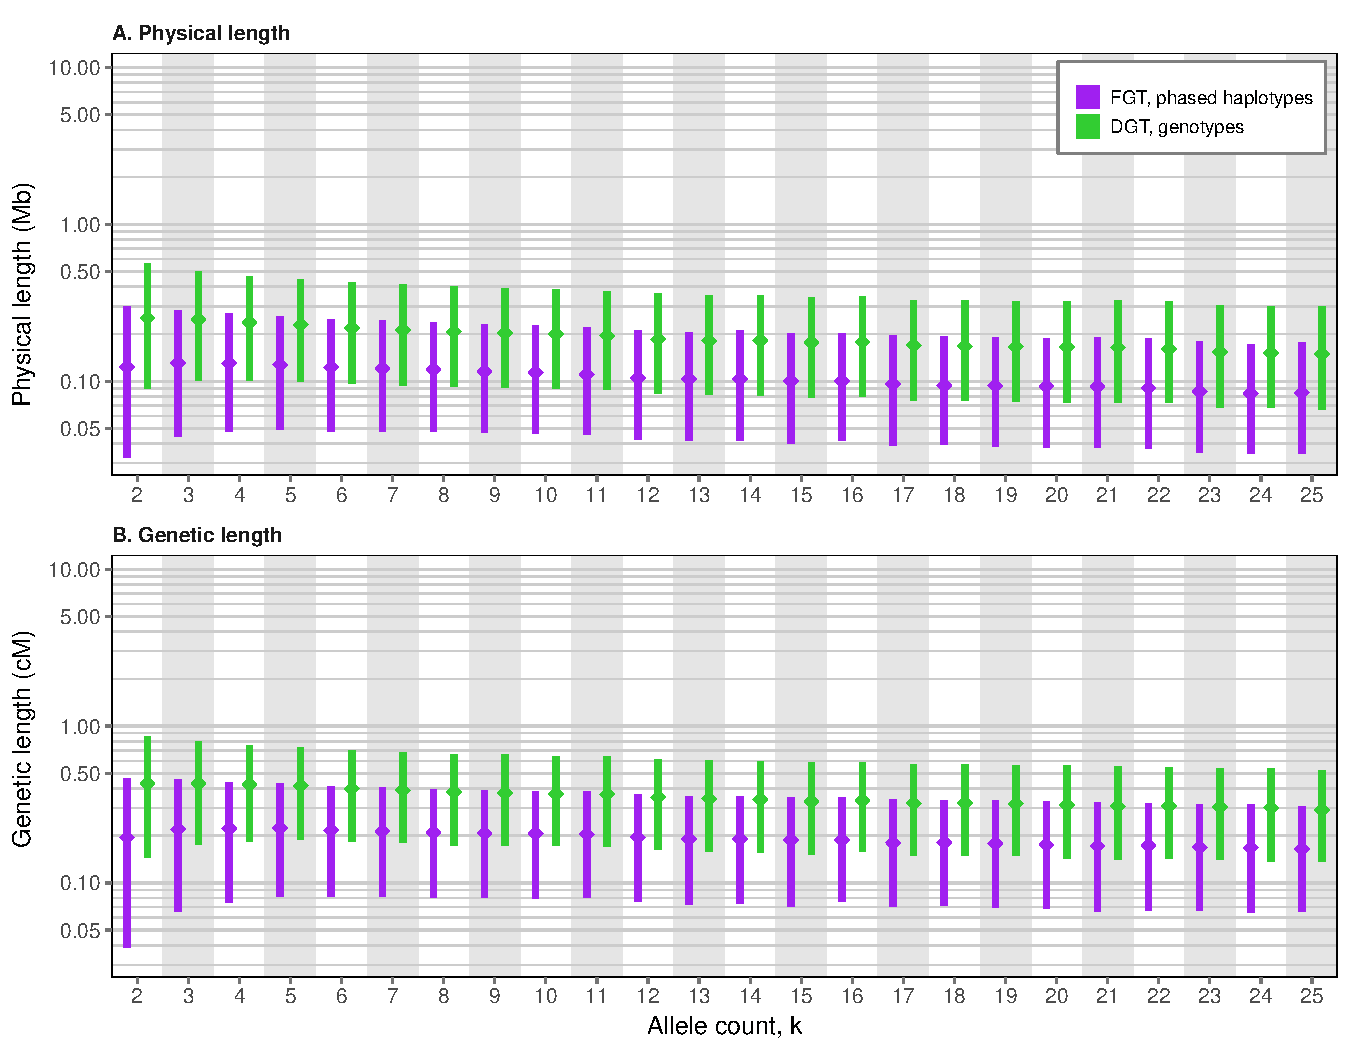
\includegraphics[width=\textwidth]{./img/ch3/length_1kg20}
\Caption{Distribution of inferred IBD lengths in 1000 Genomes data, chromosome 20}
{Results are shown for the detected physical and genetic lengths of shared haplotype segments by \fk{}, using chromosome 20 in the final release dataset of \glsentrylong{1kg} Phase~\rom{3}, including ${N = \num{2504}}$ individuals.
IBD segments were detected using the \gls{fgt} (on phased haplotypes) and the \gls{dgt} (on genotype data).
Bottom and top of each bar represent the \nth{1} and \nth{3} quartile, respectively, between which the median (\nth{2} quartile) is marked (\emph{diamonds}).}
{fig:1kg20_lengths}
\end{figure}

%

As there is no ``truth'' dataset that could serve as a reference to measure accuracy, the following analysis was limited to the quantitative description of the inferred IBD lengths.
These results are shown in \cpref{fig:1kg20_lengths}.
Median physical length (and median genetic length) over the whole set of retained IBD segments was
\SI{0.101027}{\mega\basepair} (\SI{0.1878143}{\centi\morgan}) using the \gls{fgt} and
\SI{0.179916}{\mega\basepair} (\SI{0.3393392}{\centi\morgan}) using the \gls{dgt}.
As was seen in the analysis of simulated data, the \gls{dgt} generally is more likely to overestimate breakpoint distance, leading the the discovery of longer intervals.
This discrepancy in length was more pronounced for \fk{2}~variants, for which median length was
\SI{0.1236930}{\mega\basepair} (\SI{0.1947293}{\centi\morgan}) using the \gls{fgt} and
\SI{0.2528860}{\mega\basepair} (\SI{0.4284813}{\centi\morgan}) using the \gls{dgt}.
Notably, IBD lengths were more than twice as long in half of the detected segments using the \gls{dgt}, compared to the \gls{fgt}.
The length of segments identified at lower frequencies was longer in comparison to higher frequencies; \eg for \fk{25}~variants, median length was
\SI{0.0843340}{\mega\basepair} (\SI{0.1647307}{\centi\morgan}) and
\SI{0.1492150}{\mega\basepair} (\SI{0.2918440}{\centi\morgan}) using the \gls{fgt} and \gls{dgt}, respectively.
However, the IBD lengths were highest at \fk{[3,5]} when the \gls{fgt} was used, but which was not the case for the \gls{dgt}.



--

In the simulation analysis, ...
a ratio of \dec{36.58675} detected segments per target allele on average,
and \dec{9.750788} and \dec{9.39432} for dgt, fgt* after removing duplicate segments
but \dec{30.116861} in the analysis of \gls{1kg}, chromosome~20.
and \dec{} after removing duplicate segments

ratio median physical (genetic) length of dgt/fgt* was \dec{1.380145} (\dec{1.383059}) in the simulation analysis
\dec{1.1251870} (\dec{1.1185651}) at \fk{2}~variants
but \dec{1.764705} (\dec{1.86263}) here, and \dec{2.040322} (\dec{2.1948717}) at \fk{2}~variants.

--



\DeleteNote{Section ``Inference of the shared haplotype sequence''}
%
% %
% \subsubsection{Inference of the shared haplotype sequence}
% %
%
% The IBD-based phasing concept described in \cpref{sec:ibd_phasing} was explored in this section.
% Given the genealogical constraints that follow from the assumption that the genealogy does not change along the sequence within a given breakpoint interval, it is straightforward to derive the sequence of the shared haplotype.
% This applies to sites where exactly \n{1} genotype is heterozygous and \n{1} is homozygous in a pair of individuals.
% In the following, such heterozygous-homozygous sites are referred to as being \emph{informative}, as opposed to sites where both genotypes are heterozygous, which are referred to as being \emph{indeterminate}.
% At sites where both genotypes are homozygous, phasing is trivial.
% Hence, phasing is attempted at heterozygous sites along the sequence.
%
% The analysis was performed on the full set of IBD segments detected using the \gls{dgt} in the simulated dataset; recall that the \gls{fgt} requires (phased) haplotypes and cannot be used on genotype data.
% Also, note that breakpoint sites delimit the interval enclosing a haplotype that is shared by descent, but they themselves represent the first positions along the sequence at which haplotype sharing was broken through recombination; hence, breakpoint sites were excluded from the inference.
% The purpose of this evaluation was to determine the proportions of correctly and incorrectly phased sites, as well as the proportion of indeterminate sites.
% This was then compared to the same haplotypes inferred using the set of true IBD segments.
%
% In the following, \n{2} approaches were explored; first, haplotype inference was performed separately per IBD segment and, second, the segments identified by the same shared allele were grouped and a majority-rule was applied to determine the shared haplotype sequence (referred to as \emph{consensus} approach).
% The latter represents an attempt to increase the number of informative sites, as these may differ if more pairs of individuals are considered.
% Since they share the same focal allele, it is assumed that this allele identifies the same haplotype in all pairs.
%
% %
% %!TEX root = ../../main.tex


\begin{figure}[!htb]
\centering
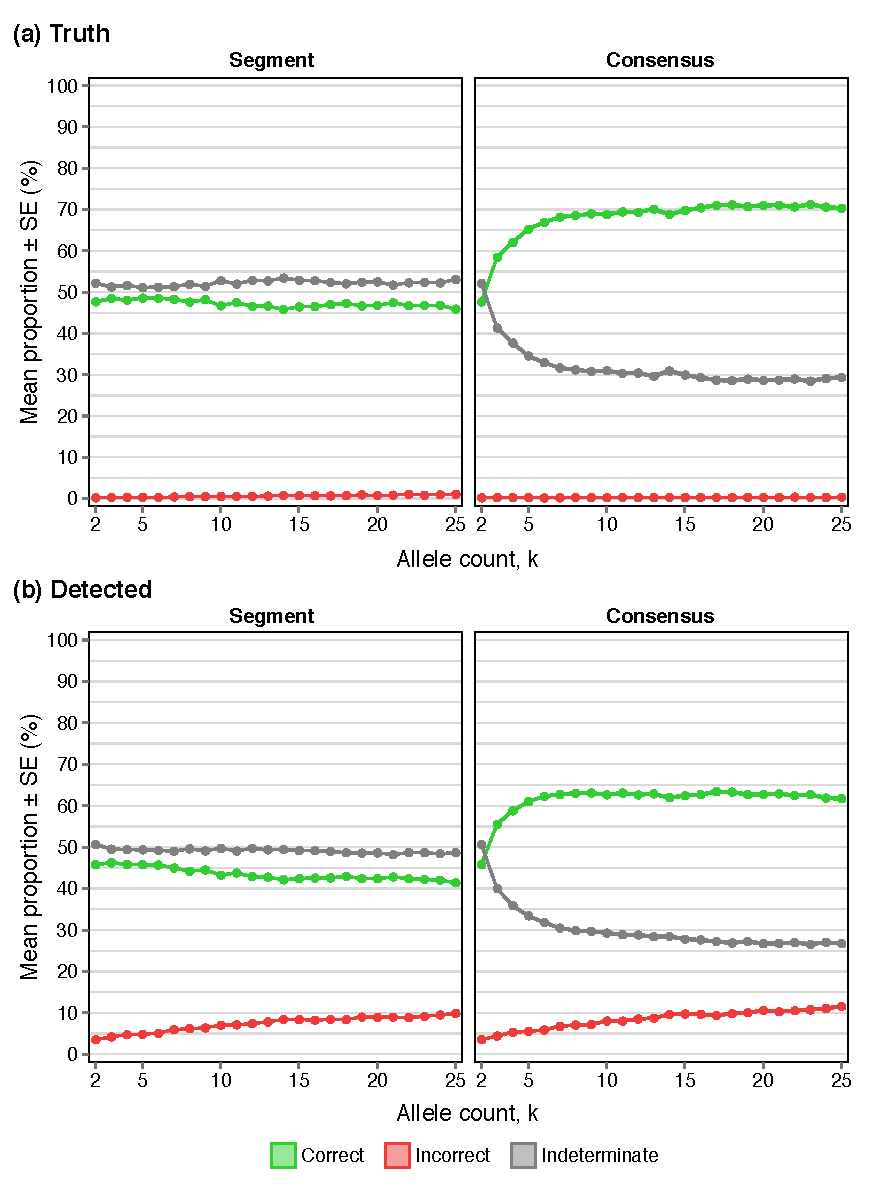
\includegraphics[width=0.75\textwidth]{./img/ch3/phase_fk_prop}
\Caption{Accuracy of alleles inferred through IBD-based phasing by focal allele frequency}
{IBD segments were randomly selected; \n{10000} per \fk{}~category.
Genotypes within each segment were phased and the relative proportions of correct, incorrect, and indeterminate alleles were recorded and averaged ($\pm\text{SE}$) per \fk{}~category.
This was done separately per segment (\emph{left}) and using the consensus approach (\emph{right}).
The results shown in Panel~\textbf{(a)} correspond to the ``truth'', where the true IBD segments were used to delimit the extent of the inferred shared haplotype sequence.
This is compared to Panel~\textbf{(b)}, where the \gls{dgt} was used to detect IBD breakpoints in genotype data.}
{fig:phase_fk_prop}
\end{figure}

% %
%
% A random subset of \n{10000} IBD segments was drawn for each \fk{}~category from the full set of detected intervals using the \gls{dgt} in which the shared haplotype was inferred.
% Similarly, for the consensus approach, target sites were randomly drawn for the set of identified targets for each \fk{}~category, such that the total number of identified segments did not exceed \n{10000} per \fk{}~category.
% Haplotypes were then inferred and combined in each focal group by applying a majority-rule to estimate the sequence of the shared haplotype.
% For each segment, the proportions of correctly inferred, incorrectly inferred, or indeterminate alleles was then determined per \fk{}~category.
% Additionally, to compare these results to the ``truth'', the same subsets of IBD segments was analysed in each approach, but where estimated haplotype length was delimited by the corresponding true IBD segments.
% The same was done for both approaches, but using the set of true IBD segments to delimit the haplotype sequence.
% The results of this analysis are shown in \cpref{fig:phase_fk_prop}.
%
% When true IBD segments were used, \cref{fig:phase_fk_prop}{a}, the proportion of incorrectly phased sites was consistently low along the allele frequency range; however, note that this proportion was not equal to zero.
% In comparison, the proportion of error increased towards higher allele frequencies when IBD was detected using the \gls{dgt}, \cref{fig:phase_fk_prop}{b}, which was seen in both the segment-based approach and the consensus approach.
% Notably, the proportion of indeterminate sites was consistently close to $50\%$ in the segment-based approach using both true and detected data.
% However, the proportion of correctly phased genotypes decreased towards higher allele frequencies; from \SI{46.173}{\percent} at \fk{2}~variants to \SI{42.330}{\percent} at \fk{25}~variants.
% In the consensus approach, the proportion of correctly phased genotypes showed a rapid increase but then reached a plateau around $70\%$ in when true IBD segments were used, and between $60\%$ and $65\%$ when detected segments were used.
%
% %
% %!TEX root = ../../main.tex


\begin{figure}[!htb]
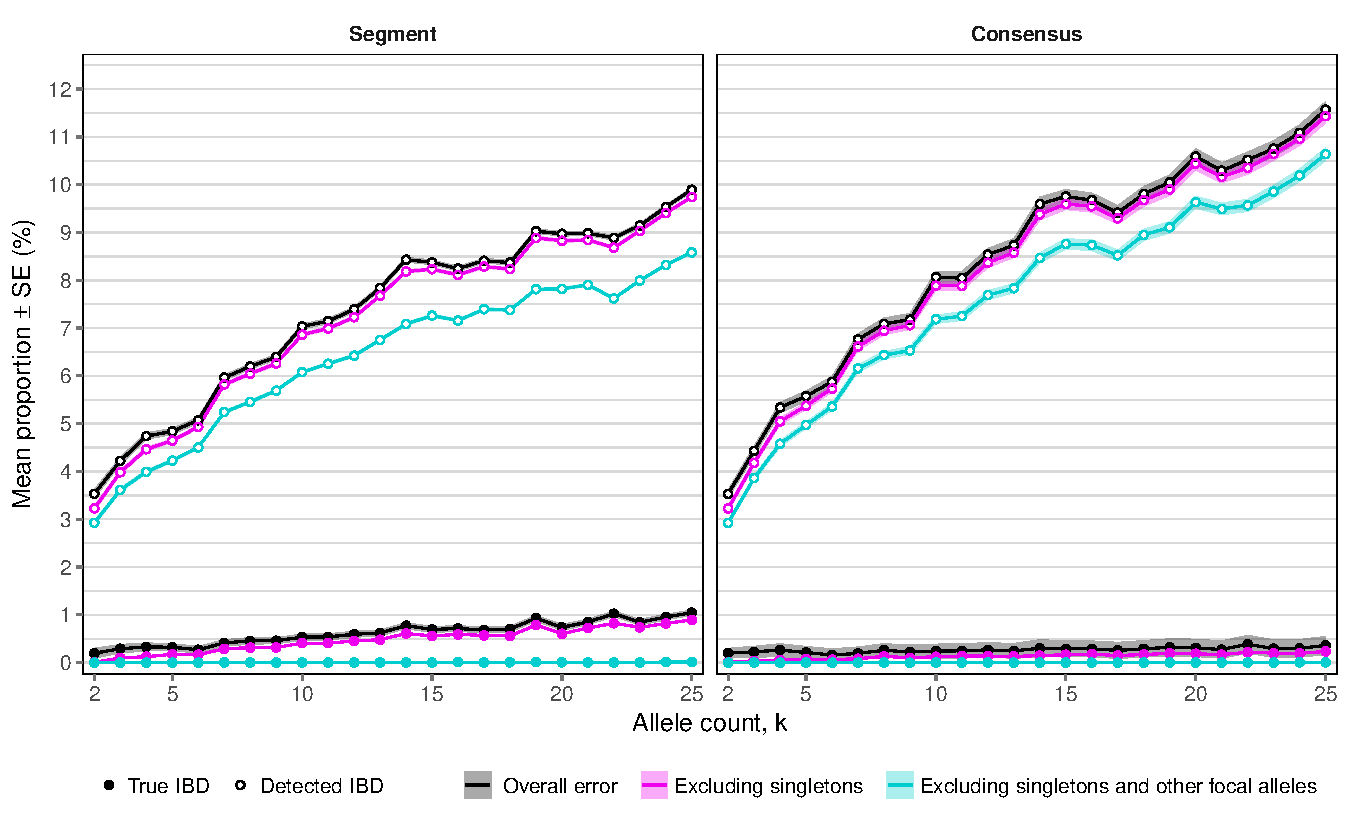
\includegraphics[width=\textwidth]{./img/ch3/phase_fk_error}
\Caption{Error distribution of alleles inferred through IBD-based phasing}
{The same results are shown as in \cref{fig:phase_fk_prop}, but with focus on incorrectly inferred alleles only; \ie the proportion of overall error corresponds to the proportion of incorrect alleles in \cref{fig:phase_fk_prop}.
The source of error was further

}
{fig:phase_fk_error}
\end{figure}

% %
%
% The distribution of incorrectly phased genotypes was further analysed to distinguish error due to singletons and other focal alleles that fell within the intervals of the segments analysed.
% These results are shown in \cpref{fig:phase_fk_error}.
% Note that in both, the exclusion of singletons did not markedly reduce the overall proportion of incorrectly phased genotypes.
% In both the segment-based approach and the consensus approach, error was noticeably reduced if genotypes at other focal variants were excluded.
% Importantly, by excluding singletons and other focal alleles that fell within the interval of the segments analysed, error was reduced to zero when true IBD segments were used.
% In fact, incorrectly phased genotypes only occurred within the overestimated regions of detected IBD segments; \ie using the \gls{dgt}.
%
% This finding is important as it suggests that haplotypes could be determined correctly if overestimation in the detection of breakpoints could be reduced or excluded.
% For example, instead of considering the full length of the segments detected, genotype phase could be determined from a narrow interval around a given target site.
%


\DeleteNote{Section ``Phasing coverage of pairwise shared haplotypes per individual''}
%
% %
% \subsubsection{Phasing coverage of pairwise shared haplotypes per individual}
% %
%
% Although the presented IBD-based phasing approach attempted to only determine genotype phase locally, it may nonetheless be of interest to explore the possibility to phase individuals ``globally''; that is, to distinguish haplotypes from genotype data along the full length of a chromosome per individual.
% To this end, it is relevant to determine the coverage of shared haplotypes along a chromosome per individual.
% Since simulated data may not be suited to derive expectations that would apply to reality, the following analysis was conducted on data from the \glsentrylong{1kg} Phase~\rom{3}, chromosome~20.
%
% I randomly selected \n{500} of the \n{2504} individuals and, for each individual, I identified all other individuals (in the whole sample of \n{2504} individuals) which shared any rare allele at \fk{[2,25]} with a given individual.
% The average number of rare alleles shared between a given individual and any other individual was \MeanValue{15234.930}{455.259586}, and the average number of unique individuals who shared any rare allele with a given individual was \MeanValue{1396.796}{9.654698}, which ranged between \n{888} and \n{1978}.
% The \gls{dgt} was used to detect segment breakpoints per pairwise shared focal allele; for comparison, the same was done using the \gls{fgt}, although only the \gls{dgt} would be applied in the context of genotype phasing.
%
% %
% %!TEX root = ../../main.tex


\begin{figure}[!htb]
%{\smaller\texthv{\textbf{A. Simulated sample}}}\\
%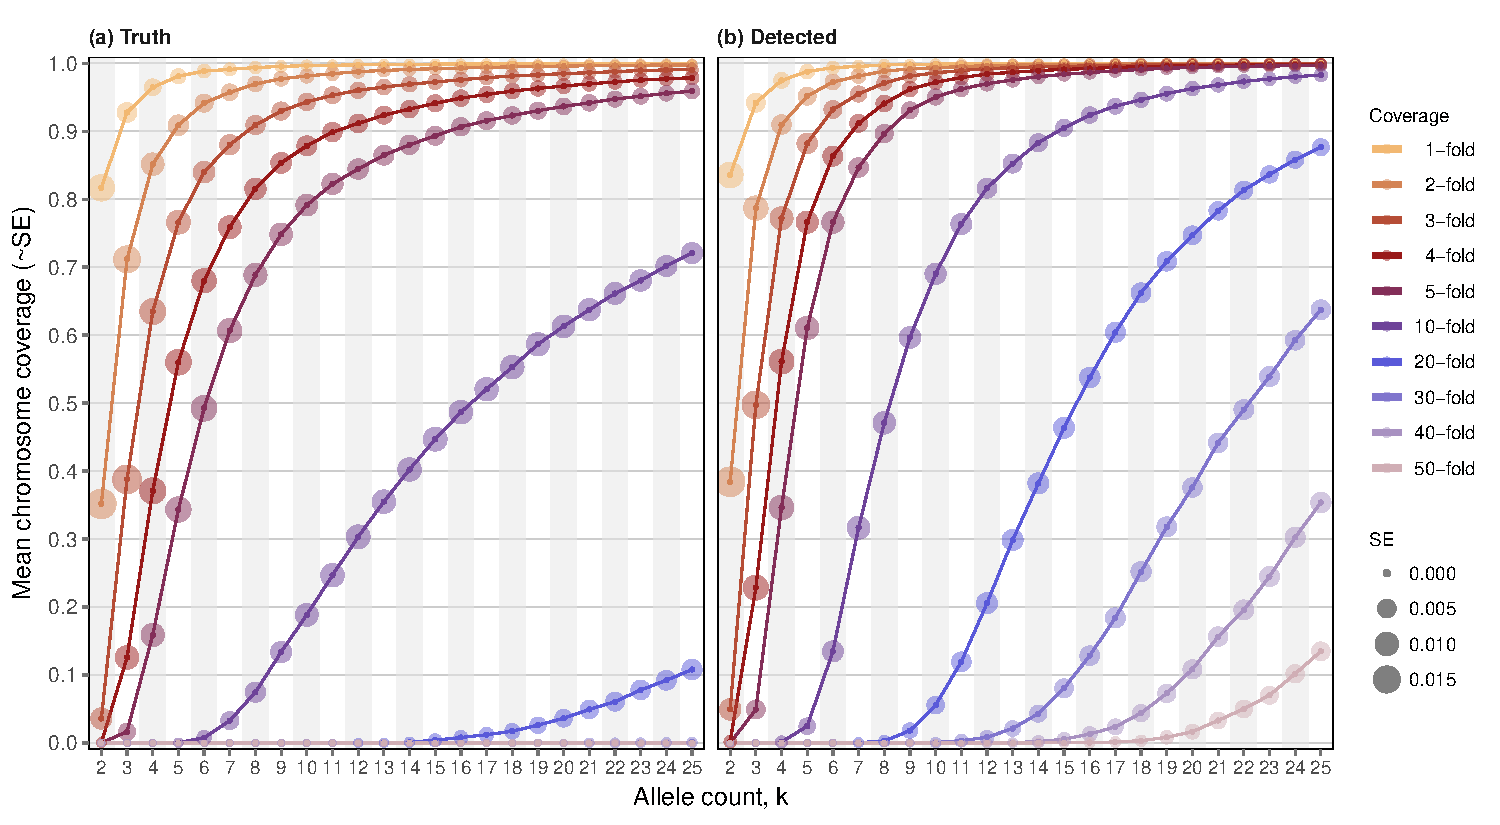
\includegraphics[width=\textwidth]{./img/ch3/phase_fk_coverage}
%{\smaller\texthv{\textbf{B. 1000 Genomes, chromosome 20}}}\\
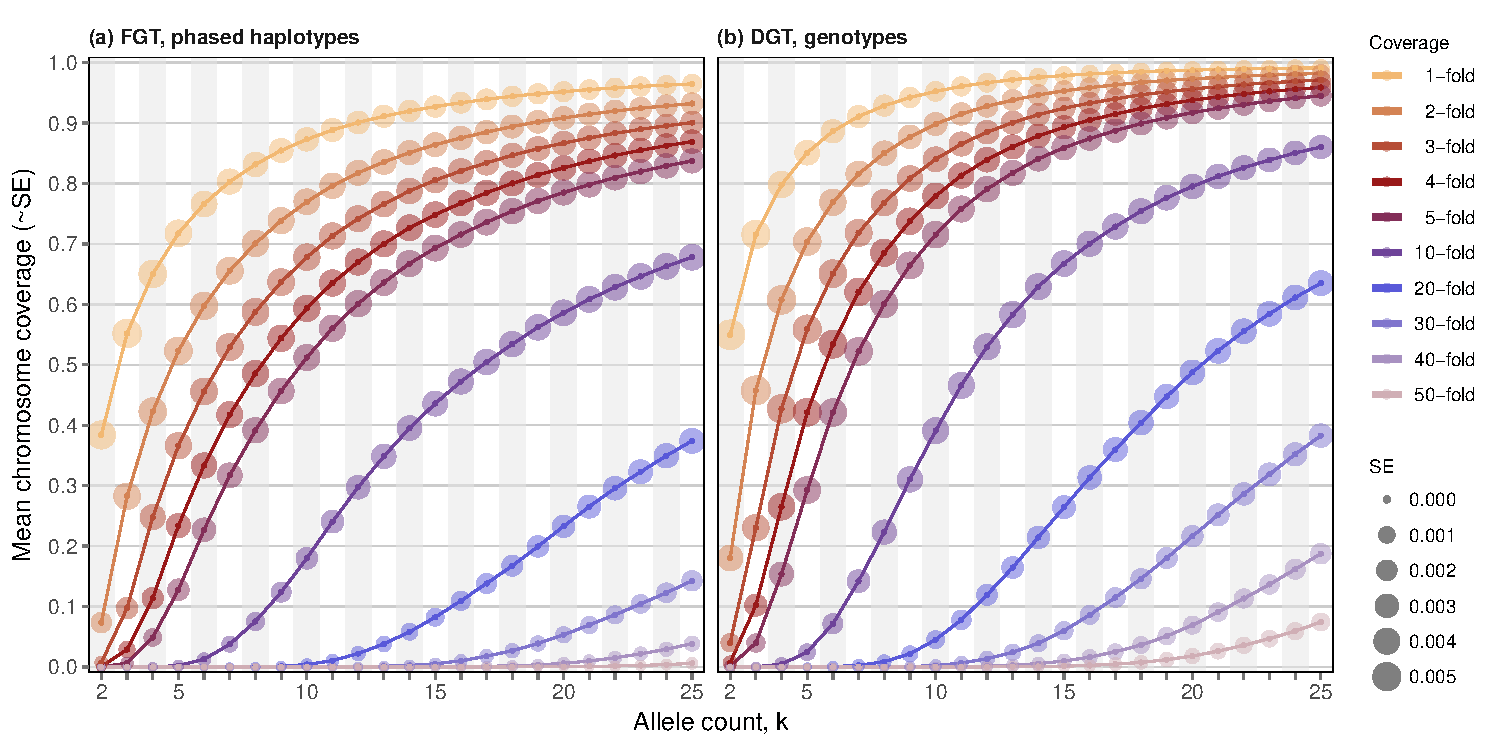
\includegraphics[width=\textwidth]{./img/ch3/phase_coverage_1kg}
\Caption{Cumulative shared haplotype coverage by focal allele count in 1000 Genomes data}
{Results are shown for \n{500} randomly selected individuals, among ${N=\num{2504}}$ in the \gls{1kg} dataset.
% (\textbf{A}), and among the ${N=\num{2504}}$ individuals in 1000 Genomes data, chromosome~20 (\textbf{B}).
Segments detected using the \gls{fgt} (\text{a}, \emph{left}) are compared to the segments detected using the \gls{dgt} (\text{b}, \emph{right}).
%In~B, for comparison, the \gls{fgt} is compared to the \gls{dgt} in the 1000 Genomes dataset.
Coverage was defined as the proportion of chromosome length covered by inferred and aligned shared haplotypes, where $n$-fold indicates that the chromosome was covered $n$-times by all segments up to a given \fk{}~category (hence, cumulative).
\Gls{se} is indicated by the size of dots (see figure legend).}
{fig:phase_fk_coverage}
\end{figure}

% %
%
% Each set of detected segments was then reduced to include only unique IBD intervals; again after sorting by focal allele frequency such that the focal allele is the one with lowest frequency within a given segment.
% Recall that duplicate segments refer to IBD intervals that are tagged by multiple \fk{}~variants, which are assumed to sit on the same underlying shared haplotype.
% The average number of unique segments retained per individual was \MeanValue{5071.224}{79.976994} for the \gls{dgt} and \MeanValue{5460.694}{85.317616} for the \gls{fgt}; note that haplotype data were phased.
% Retained haplotype segments were aligned by position along the chromosome to measure coverage, \ie the proportion of the chromosome covered.
% Mean coverage across all \n{500} randomly selected individuals is given in \cpref{fig:phase_fk_coverage}, which indicates the $n$-fold cumulative coverage by \fk{}~category; shown for true IBD segments (\cref{fig:phase_fk_coverage}{a}) and segments detected using the \gls{dgt} (\cref{fig:phase_fk_coverage}{b}).
%
% Coverage was overall higher for the \gls{dgt} compared to the \gls{fgt}, due to overestimating IBD lengths.
% Notably, neither the \gls{dgt} nor the \gls{fgt} reached full coverage on average.
% However, a steady increase was seen when \fk{}~variants at higher frequency were included.
% Considering \fk{2}~variants alone, the \gls{dgt} reached ${>50\%}$ 1-fold coverage, which was higher compared to the \gls{fgt} with ${< 40\%}$ 1-fold coverage.
% Considering focal alleles occurring at higher frequencies, the \gls{dgt} was at ${\approx 99\%}$ 1-fold cummulative coverage at \fk{\leq 20}, whereas the \gls{fgt} slowly approached ${\approx 95\%}$ 1-fold cummulative coverage at \fk{\leq 25}.
%
% These results indicate that a ``global'' phasing approach using inferred IBD information alone would not be able to fully determine haplotypes in sample data of unrelated individuals.
% However, note that similar approaches have been applied to sets of related individuals, for which it can be expected that there are more and longer pairwise shared haplotypes; \ie \glsentryfull{lrp} methods \citep{Kong:2008gh,Palin:2011cl,loh2016fast}.
%



%
\section{Discussion}
%


In this chapter, I presented a novel IBD detection method which is able to infer recombination events in both haplotype and genotype data.
To be able to apply this method on a larger scale, I implemented the IBD detection algorithm described in this chapter as a computational tool written in \cpp; called \textbf{\texttt{tidy}} (\underline{t}argeted \underline{I}BD \underline{d}etection done thoroughl\underline{y}).\footnote{Targeted IBD detection done thoroughly, \texttt{tidy}: \url{https://github.com/pkalbers/tidy}}
% I applied the \texttt{tidy} algorithm to all autosomes in the \gls{1kg} dataset, in which I included all rare allele \glspl{snp} observed below a $0.5$\% allele frequency threshold (\ie \fk{}~variants with ${k \in [2, 25]}$).
% This was done using both the \gls{fgt} and the \gls{dgt}; the results are available online.\footnote{Download ???}

Although the \gls{fgt} showed overall high levels of accuracy, phasing error was identified as a problem.
Current phasing methods such as \texttt{SHAPEIT\,2} typically show very low error rates \citep{OConnell:2014fl}.
However, occasionally, alleles are placed on the wrong haplotype.
This may happen at single loci (\emph{flip~errors}) or such that longer haplotype stretches are exchanged (\emph{switch~errors}).
Both types of error can affect breakpoint detection under the \gls{fgt} as both flip and switch errors may change the configuration of alleles observed in relation to a given focal variant.
As an alternate solution to using phased haplotypes, the \gls{dgt} can be used on genotype data, which is therefore not affected by phasing error.
However, the lengths of detected IBD segments tend to be overestimated.

Notably, the IBD results obtained from analysis of the \gls{1kg} dataset suggests that the \gls{fgt} was similarly affected by phasing error as seen in the simulation analysis.
However, the \gls{dgt} was also affected by other sources of error.
One consideration is that both the \gls{fgt} and \gls{dgt} assume the infinite sites model, but this is only an approximation of conditions observable in nature.
In particular, back mutations and recurrent mutations are excluded in the model, but these are prevalent in the (human) genome.
For instance, recurrent mutations can produce patterns of variation that would otherwise only be observable if recombination had occurred \citep{McVean:2002ws}.
Thus, false positive breakpoints may be inferred, such that IBD length is underestimated.
Nonetheless, the infinite sites model is usually seen as a reasonable approximation to reality, as the number of variant sites in a sample is typically much smaller than the number of nucleotides in the chromosomal sequence \citep{hein2004gene}.
However, the presence of genotype error cannot be ruled out and therefore requires further consideration.


\Delete{
Lastly, the IBD-based phasing concept showed that that it is possible to derive the shared allelic state sequence in pairs of individuals that share a haplotype by descent.
This approach, in its current implementation, is only able to phase genotype data over locally shared segments.
However, a potential utility of such a local phasing approach may arise considering that rare variants can be used to identify recent relatedness patterns in large datasets.
Because a given rare allele identifies the underlying shared haplotype, the inferred sequence is likely to correctly distinguish the haplotypes of an individual within a shorter region around the target position.
For example, this information may serve as a \emph{post-hoc} correction to haplotype data produced using existing phasing methods.
}

% !TEX root = ../main.tex

\glsresetall


\topquote[9cm]{
The first principle is that you must not fool yourself --\\
and you are the easiest person to fool.}
{Richard Feynman}

{
\singlespacing
\chapter{Consideration of genotype error in the inference of haplotype sharing by descent}
\label{ch:generr}
\minitoc
}


%
\section{Introduction}
%

Recent advancements in genotyping and \gls{ngs} technologies have enabled us to study the human genome in unprecedented detail and scale.
The availability of high-throughput methods to survey large samples has led to successful identification of thousands of disease causing risk factors, which in particular was driven by \gls{gwa} studies.
This explosion of human genetic data has further enabled collaboration initiatives through the setup of genetic databases, which can be queried by research groups worldwide.
However, because no technology is perfect, acquired data are likely to contain undetected amounts of error, which may affect statistical inference in many ways.

Statistical tests often rely on the assumption that genotype data (retained after quality control) are correct, or that error quantities are negligible.
Yet, the effects of misclassification in genotype data are well documented.
For example, it has been shown that even minor amounts of genotype error can distort estimated distances in linkage mapping studies \citep{Buetow:1991wc,Shields:1991uw,Sobel:2002}, result in a substantial loss of linkage information in quantitative trait analyses \citep{Douglas:2000hb,Abecasis:2001jp}, decrease power in association studies \citep{Kang:2004hy}, and can substantially increase type I (false positive) error in haplotype-based case-control analyses \citep{moskvina2005minor}.

Identification of incorrectly typed or called genotypes remains a difficult problem, which becomes more challenging as the magnitude of data increases.
But, for example, as shown by \citet{Cox:2006kv} and independently by \citet{Moskvina:2006fz},
genotype error \Addition{theoretically} does not always affect the distributions of genotypes to the extent that \gls{hwe} can be violated.
\Correct{Given the common practise to exclude presumably incorrect genotypes based on departures from \gls{hwe}, it therefore remains difficult to catch falsely called or typed variants.}


In this chapter, I explore the impact of genotype error on the detection of \gls{ibd} segments and, based on these results, I implement a new approach for targeted IBD inference using a \gls{hmm}.
First, I introduce a generic model for genotype error; see section below.
The remainder of this chapter is then divided into \n{2} main parts.
In the first part (\cref{sec:generrprofiles}), I characterise the distribution of genotype error in data obtained on different genotyping and sequencing platforms, to construct empirical error profiles.
I use this information to integrate realistic error rates in simulated data, such that the effects of error can be observed in practice.
In particular, I evaluate the non-probabilistic IBD detection method presented in Chapter~3.
The insights gained from this analysis enabled a probabilistic extension of the targeted IBD detection method, which I implemented using a \gls{hmm}; I present this new method in the second part of this chapter (\cref{sec:ibd_hmm_method}).
This HMM-based method is incorporated in the previously presented \texttt{tidy} algorithm for the targeted detection of IBD segments (see Chapter~3).




%
\subsection{Probability of genotype error}
\label{sub:probgenerr}
%

Consider a biallelic locus with alleles $a$~or~$b$, which respectively occur at frequency $p$ and ${q = 1 - p}$ in a population.
Genotypes are formed by combination of \n{2} alleles in diploid organisms (therefore sometimes referred to as \emph{diplotypes}).
There are \n{4} possible combinations of alleles, \ie $aa$, $ab$, $ba$, and $bb$, but of which genotypes $ab$ and $ba$ are indistinguishable.
It is convenient to recode the \n{2} alleles as 0~and~1 to denote the reference and alternate allele, respectively.
By introducing $k$ to count the number of alternate alleles, let $g_{k}$ denote a genotype, where ${k \in \lbrace 0, 1, 2 \rbrace}$.
% Allele frequency can now be expressed as
% \begin{equation}\label{eq:happropk}
% 	f_h(c) = p^{1-c} q^c \text{.}
% \end{equation}
If all combinations of the \n{2} alleles are statistically independent, \eg in a randomly mating population, sample genotype frequencies, ${f_{g}(k)}$, are multinomially distributed with expectations given by \gls{hwe} proportions \citep{Hardy:1908wx, Weinberg:1908tr}; \ie such that ${(p+q)^2 = p^2 + 2pq + q^2 = 1}$.
% which is commonly known as the Hardy-Weinberg principle \citep{Hardy:1908wx, Weinberg:1908tr}.
The general form of the expected genotype frequency is given in \cref{eq:genpropk}, where $n$ refers to the number of chromosome copies (ploidy); \eg ${n = 2}$ for diploid organisms.
\begin{equation}\label{eq:genpropk}
	f_{g}(k) = {{n}\choose{k}}~p^{n-k}~q^{k}
\end{equation}

In presence of genotype error, the actual, \emph{true} genotype is distinguished from the \emph{observed} genotype, $\tilde{g}_k$, and the observed frequency, ${f_{\tilde{g}}(k)}$, is different from the true (but unknown) genotype frequency, dependent on the rate of error.
More precisely, let the rate at which genotype $g_j$ is classified as $\tilde{g}_i$ be denoted by $\varepsilon_{ij}$, where ${i,j \in \lbrace 0, 1, 2 \rbrace}$.
The value of $\varepsilon_{ij}$ is often referred to as the \emph{penetrance} of a genotype and represents the probability of observing genotype~$\tilde{g}_i$ given the true genotype~$g_j$ \citep{ott1999analysis,Gordon:2002cz}.
\Addition{In the following, I use the term \emph{error~rate} to refer to genotype penetrance.}
For convenience, \Correct{error rate} parameters can be represented in a ${3 \times 3}$ confusion matrix, $\mathcal{E}$, below.
\begin{equation}\label{eq:errormatrix}\onehalfspacing
\mathcal{E} =
\begin{bmatrix}
	\varepsilon_{00}  &  \varepsilon_{01}  &  \varepsilon_{02}  \\
	\varepsilon_{10}  &  \varepsilon_{11}  &  \varepsilon_{12}  \\
	\varepsilon_{20}  &  \varepsilon_{21}  &  \varepsilon_{22}
\end{bmatrix}
\end{equation}

Considering the relation ${\sum_{i=0}^{2} \varepsilon_{ij} = 1 ~ \forall ~ j}$, where ${0 \leq \varepsilon_{ij} \leq 1}$, it follows that the expected observation frequency of a genotype is
\begin{equation}\label{eq:errfrqprob}\onehalfspacing
f_{\tilde{g}}(k) ~=~
\begin{cases}
~	f_g(0)~\varepsilon_{00} ~+~
	f_g(1)~\varepsilon_{01} ~+~
	f_g(2)~\varepsilon_{02}  &  \text{if} ~ k = 0 \\
~	f_g(0)~\varepsilon_{10} ~+~
	f_g(1)~\varepsilon_{11} ~+~
	f_g(2)~\varepsilon_{12}  &  \text{if} ~ k = 1 \\
~	f_g(0)~\varepsilon_{20} ~+~
	f_g(1)~\varepsilon_{21} ~+~
	f_g(2)~\varepsilon_{22}  &  \text{if} ~ k = 2 \\
\end{cases}
\end{equation}
where $i=j$ indicates correct classification and $i \neq j$ misclassification of the true genotype; see \citet{Moskvina:2006fz}.


%
\subsubsection{Genotype error models}
%

\Cref{eq:errormatrix,eq:errfrqprob} provide a generic framework for the \Correct{error rate} of genotypes and the calculation of genotype frequencies after error.
\N{2} \Correct{error} models are presented below which provide formulations for the calculation of model parameters $\varepsilon_{ij}$.

\citet{Douglas:2002hp} introduced a genotype-based model with parameters $\gamma$ and $\eta$, denoting the probability of a homozygous genotype to be misclassified as a heterozygous genotype and vice-versa, respectively.
The intuition behind this model is based on technical error in the \gls{pcr} amplification process, which is used in both genotyping and sequencing methods for the replication of DNA fragments.
However, note that observed genotypes $\tilde{g}_0$ and $\tilde{g}_2$ both have equal probability to arise from misclassification of $g_1$, and the probability that a homozygous genotype appears as the opposite homozygote, $g_0$ as $\tilde{g}_2$ or $g_2$ as $\tilde{g}_0$, is zero.

As an alternative, misclassification of genotypes can be modelled as a consequence of errors that occur at random and independently in each of the \n{2} alleles.
An explicit formulation of an allele-based model was proposed by \citet{Gordon:2001im}, where $\epsilon_0$ was defined as the probability that allele~0 ($h_0$) was observed as allele~1 ($h_1$), and $\epsilon_1$ the probability that $h_1$ was observed as $h_0$.

%
% !TEX root = ../../main.tex


\begin{table}[!htb]
\Caption{Penetrance functions in genotype and allele-based error models}
{Error probability (or \emph{penetrance}) is denoted by $\varepsilon_{ij}$, which is the probability of observing genotype~$i$ given the true genotype~$j$.
\N{2} models are presented which are genotype-based and allele-based, respectively.
In each model, equations refer to the probability that a true genotype, $g_j$, was observed as any of the possible genotypes, $\tilde{g}_i$, such that $\varepsilon_{ij}$ is calculated from the corresponding row-by-column expression.
}
{tab:errormodel}
\centering
\begin{threeparttable}
\renewcommand{\arraystretch}{1.1}%
\begin{tabular}{lcccc}
\toprule
Model & Observed genotype & \multicolumn{3}{c}{True genotype} \\ \cmidrule(lr){3-5}
  &  & $g_0$ & $g_1$ & $g_2$ \\ \midrule
\textbf{Genotype-based$^1$}
& $\tilde{g}_0$ &  $1 - \gamma$ &  $\tfrac{1}{2}\eta$ &  $0$          \\[1.2ex]
& $\tilde{g}_1$ &  $\gamma$     &  $1 - \eta$         &  $\gamma$     \\[1.2ex]
& $\tilde{g}_2$ &  $0$          &  $\tfrac{1}{2}\eta$ &  $1 - \gamma$ \\ \midrule
\textbf{Allele-based$^2$}
& $\tilde{g}_0$
	&  ${(1 - \epsilon_0)^2}$
	&  ${\epsilon_1 (1 - \epsilon_0)}$
	&  ${\epsilon_1}^2$  \\[1.2ex]
&  $\tilde{g}_1$
	&  ${2 \epsilon_0 (1 - \epsilon_0)}$
	&  ${\epsilon_0 \epsilon_1 + (1 - \epsilon_0)(1 - \epsilon_1)}$
	&  ${2 \epsilon_1 (1 - \epsilon_1)}$  \\[1.2ex]
&  $\tilde{g}_2$
	&  ${\epsilon_0}^2$
	&  ${\epsilon_0 (1 - \epsilon_1)}$
	&  ${(1 - \epsilon_1)^2}$  \\ \bottomrule
\end{tabular}
\begin{tablenotes}\footnotesize
	\item[1] \citet{Douglas:2002hp};
	\quad $\gamma = P(\text{hom.} \rightarrow \text{het.})$,
	\quad $\eta = P(\text{het.} \rightarrow \text{hom.})$
	\item[2] \citet{Gordon:2001im};
	\quad $\epsilon_0 = P(h_0 \rightarrow h_1)$,
	\quad $\epsilon_1 = P(h_1 \rightarrow h_0)$
\end{tablenotes}
\begin{tablenotes}[para]\footnotesize
Table modified from \citet{Gordon:2002cz}, Table~2.
\end{tablenotes}
\end{threeparttable}
\end{table}

%

%
% !TEX root = ../../main.tex


\begin{figure}[!htbp]
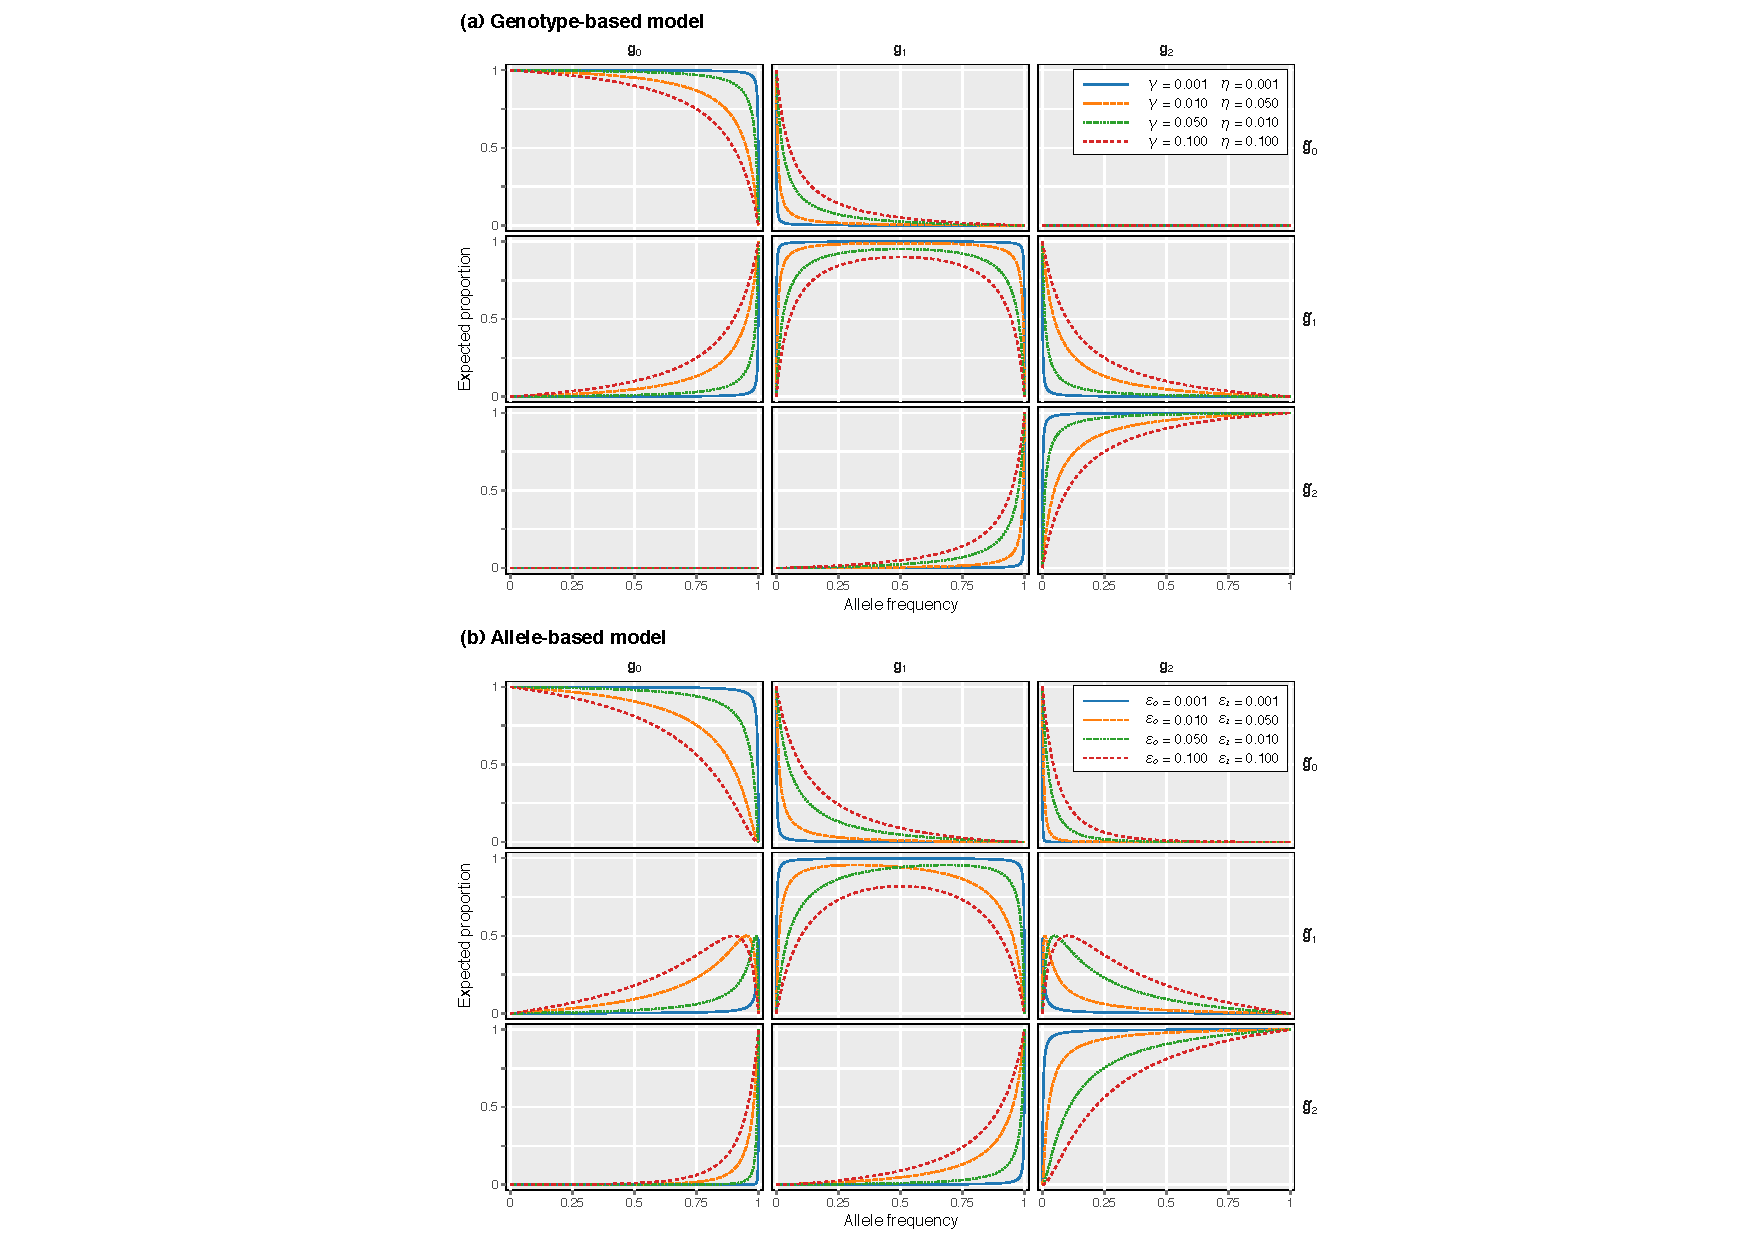
\includegraphics[width=\textwidth]{./img/ch4/error_models}
\Caption{Expected proportions of genotype error for the genotype and allele-based models}
{The graphs show the expected proportions of true genotypes ($g$) that make up an observed genotype ($\tilde{g}$) given the true allele frequency; calculated at different, nominal error rates (see legend).
The error functions provided in \cpref{tab:errormodel} were used as in \cpref{eq:errfrqprob} and results were normalised to sum to 1 per observed genotype (columns).\AdditionLabel}
{fig:error_models}
\end{figure}

%

\Correct{Error} functions for both models are given in \cpref{tab:errormodel}; note that these are arranged as in error matrix $\mathcal{E}$ in \cref{eq:errormatrix}.
\Addition{To illustrate the expectations arising from these models, \cpref{fig:error_models} shows the expected proportions of true genotypes found as a given observed genotype at different, nominal error rates, for both the genotype and allele-based models.}
\Addition{It should be noted that the error parameters specified in each model may not apply equally to each variant in genomic data, due to differences arising from technical bias in the sequencing or genotyping process and variations in the accessibility of DNA along the genome (\eg chromatin structure variations near telomeric or centromeric regions).}

In the following section, I estimated genotype \Correct{error rates} in different datasets.
In each, error was computed from the proportions of correctly and incorrectly classified genotypes, such that error parameters were estimated for each model.




%
\section{Generation of platform-specific genotype error profiles}
\label{sec:generrprofiles}
%

Assessment of genotype accuracy requires the existence of an error-free ``gold~standard'' dataset against which data generated on other platforms can be compared; provided that data were obtained on the same biological sample.
In reality, however, the possibility of undetected genotype error cannot be excluded, but it can be reduced, for example, based on pedigree information and the laws of Mendelian inheritance.
In the section below, I describe the dataset which I used as a reference for high-confidence genotype data.
These were compared to several publicly available datasets generated using different genotyping and sequencing technologies, which included individuals also present in the reference dataset.

%
\subsection{High-confidence genome data as benchmark for comparisons}
%

The analysis was based on data from the \gls{ipg},\footnote{Illumina Platinum Genomes: \url{http://www.illumina.com/platinumgenomes/} \accessed{2016}{11}{16}} which comprises a \n{17}-member, \n{3}-generation family of European ancestry; CEPH~pedigree~1463.\footnote{Centre d'Etude du Polymorphisme Humain (CEPH), Utah family pedigree 1463: \url{https://catalog.coriell.org/0/Sections/Collections/NIGMS/CEPHFamiliesDetail.aspx?fam=1463} \accessed{2016}{11}{16}}
This dataset has been generated using recent state-of-the-art sequencing technologies and methods for variant calling, where a total of 5.43~million variants were identified genome-wide \citep{Eberle:2016ki}; this included 4.73~million \glspl{snp}.
Individuals had been sequenced to a depth of 50x on Illumina HiSeq~2000, and variants were called in concordance to several variant calling methods.
Notably, due to the availability of pedigree information, artefacts such as genotype errors had been excluded based on deviations from Mendelian inheritance.
The dataset comprises \n{11} children from \n{2} parents, who themselves are the children of the \n{4} founders of the pedigree; see \cref{fig:ceph1463}.
Thus, inheritance constraints were most informative for the \n{2} parents, labelled \textsf{NA12877} and \textsf{NA12878} (Coriell~ID), which were additionally sequenced to 200x depth, and for which high-confidence variant calls were made available.

%
%!TEX root = ../../main.tex


\begin{figure}[!htb]
\centering
\vspace{5pt}
\begin{tikzpicture}[-,auto,thick,font=\sffamily\footnotesize,
F/.style={circle,draw,fill=white,ultra thick,minimum size=4mm,outer sep=3pt},
M/.style={rectangle,draw,fill=white,ultra thick,minimum size=4mm,outer sep=3pt},
mate/.style={cross out,draw=black,minimum size=2mm,inner sep=0pt,outer sep=0pt}]

\newcommand{\springoff}[2]{
\draw[-,rounded corners=5pt] (#1.south) |- (#2);
}
\newcommand{\offspring}[2]{
\path (#1) -- (#2.north) coordinate[pos=0.5] (mid);
\draw[-,rounded corners=3pt] (#1) |- (mid) -| (#2.north);
}

\node[M,fill=Ivory2] (a) at (3.25,4) {};
\node[mate]  at (4.00,4) {};
\node[F,fill=Ivory2] (b) at (4.75,4) {};
\node[M,fill=Ivory2] (c) at (6.25,4) {};
\node[mate]  at (7.00,4) {};
\node[F,fill=Ivory2] (d) at (7.75,4) {};

\coordinate (A) at (4,3.5);
\coordinate (B) at (7,3.5);

\node[M,fill=Chocolate3,label={left:NA12877}] (77) at (4,2.5) {};
\node[mate] at (5.5,2.5) {};
\node[F,fill=Chocolate3,label={right:NA12878}] (78) at (7,2.5) {};

\coordinate (P) at (5.5,2);

\node[F,fill=Ivory2] (1) at (1,1) {};
\node[F,fill=Ivory2] (2) at (2,1) {};
\node[F,fill=Ivory2] (3) at (3,1) {};
\node[M,fill=Ivory2] (4) at (4,1) {};
\node[M,fill=Ivory2] (5) at (5,1) {};
\node[M,fill=Ivory2] (6) at (6,1) {};
\node[F,fill=Ivory2] (7) at (7,1) {};
\node[M,fill=Ivory2] (8) at (8,1) {};
\node[F,fill=Ivory2] (9) at (9,1) {};
\node[M,fill=Ivory2] (10) at (10,1) {};
\node[M,fill=Ivory2] (11) at (11,1) {};


\springoff{a}{A}
\springoff{b}{A}
\draw [-] (A) to (77.north);

\springoff{c}{B}
\springoff{d}{B}
\draw [-] (B) to (78.north);

\springoff{77}{P}
\springoff{78}{P}

\offspring{P}{1}
\offspring{P}{2}
\offspring{P}{3}
\offspring{P}{4}
\offspring{P}{5}
\offspring{P}{6}
%\draw [-] (P) to (6.north);
\offspring{P}{7}
\offspring{P}{8}
\offspring{P}{9}
\offspring{P}{10}
\offspring{P}{11}

\end{tikzpicture}
\vspace{5pt}
\Caption{CEPH pedigree 1463}%
{The pedigree of the family sequenced in the \glsentrylong{ipg}.
Genotype data of individuals \textsf{NA12877} and \textsf{NA12878} (indicated) were used as reference against which data obtained on other genotyping or sequencing platforms were compared.
Figure modified from \citet{Eberle:2016ki}, Figure~1.}%
{fig:ceph1463}
\end{figure}

%

Genotype (\gls{snp}) data from \gls{ipg} for individuals \textsf{NA12877} and \textsf{NA12878} were used as reference or \emph{truth} for comparison to concordant data obtained on other platforms.
Although the possibility of genotype error in \gls{ipg} data cannot be excluded, it is assumed that error rates in \textsf{NA12877} and \textsf{NA12878} are sufficiently low to allow proportional estimation of genotype misclassification rates based on observations over thousands of variant sites.
%Likewise, the probability of double-error, if both ``true'' and ``observed'' genotypes are misclassified at single loci, was ignored as it was assumed to be negligibly small.

Due to the imperfection of even high-standard sequencing technologies, not all chromosomal regions are equally accessible, which affects the power to determine variants in the calling process along the length of the sequence.
The confidence of variant calls is derived from the depth of mapped sequence reads and quality scores.
To maintain high levels of confidence in the data, accessibility masks provided by \gls{ipg} were applied such that only sites in high-confidence regions were retained in the analysed datasets.
This retained a sum of \dec{3.407}~million and \dec{3.605}~million \glspl{snp} for \textsf{NA12877} and \textsf{NA12878}, respectively, across chromosomes~1--22.


%
\subsection{Selection and preparation of datasets from different platforms}
%

Because cell lines from CEPH~pedigree~1463 are a well-characterised model system, either \textsf{NA12877} or \textsf{NA12878}, or both, have been assessed in several studies.
For example, CEPH~pedigree~1463 was genotyped in the \glsentrylong{hapmap}, which was one of the first large-scale catalogues of human genetic variation \citep{Thorisson:2005ff,Frazer:2007kha,InternationalHapMapConsortium:2010en}.
Considering a more recent example, the \glsentrylong{1kg} provides data obtained on several platforms, including \gls{wgs} and high-density genotyping technologies \citep{Durbin:2010gj,GenomesProjectConsortium:2012co,Auton:2015gk}.

It must be noted that the process of acquiring data is substantially different for genotyping and sequencing methods.
The established approach for genotyping is to use chip or array-based methods, which are designed to target, or ``type'' specific molecular markers at predetermined regions and require prior knowledge about mapped locations in the genome.
On the other hand, sequencing determines the contiguous nucleotide sequence, either genome-wide or for a region of the genome.
Sequence data are aligned against a reference genome and further processed.
Eventually, variants are ``called'' at nucleotides that differ from the reference at each position along the sequence.
%Both types of data can be represented in \gls{vcf}.

Genotype error profiles were generated for both sequencing and genotyping data, which were taken from available resource data of the \glsentrylong{1kg}.
The following \emph{test} datasets were included:
\begin{itemize}
\item Low-coverage sequencing data from the final release of \glsentrylong{1kg} Phase~\rom{3} (\textbf{\emph{1000G}}), generated on Illumina HiSeq~2000 and HiSeq~2500 platforms (2-4x), and consisting of 78~million \glspl{snp} in total.
\item Genotyping data generated on Illumina HumanOmni2.5 BeadChip (\textbf{\emph{Omni2.5}}) with 2.46~million \glspl{snp}.
%Note that Omni2.5 does not capture variants below \gls{maf} of 2.5\%.
\item Genotyping data generated on Affymetrix Genome-Wide Human SNP Array~6.0 (\textbf{\emph{Affy6.0}}) with 0.91~million \glspl{snp}.
\end{itemize}
To acknowledge differences arising from the variant calling and filtering process in sequencing data, \n{2} \emph{1000G} profiles were created; one that included all variant sites (\textbf{\emph{1000G.A}}), and one containing only sites within high-confidence regions (\textbf{\emph{1000G.B}}).
For the latter, the ``strict'' accessibility mask provided by \glsentrylong{1kg} Phase~\rom{3} was used \citep[see][supplementary information 9.2]{Auton:2015gk}.\footnote{Accessible genome masks in 1000G: \url{http://ftp.1000genomes.ebi.ac.uk/vol1/ftp/release/20130502/supporting/accessible_genome_masks/} \accessed{2016}{11}{27}}
Note that the sample of the final release dataset of \emph{1000G} included \textsf{NA12878}, but not \textsf{NA12877}.
The other \n{2} datasets, \emph{Omni2.5} and \emph{Affy6.0}, which were part of previous releases of the \glsentrylong{1kg}, included both \textsf{NA12877} and \textsf{NA12878}.\footnote{High-density genotyping data, Omni2.5 and Affy6.0 in \gls{1kg}: \url{ftp://ftp.1000genomes.ebi.ac.uk/vol1/ftp/release/20130502/supporting/hd_genotype_chip/} \accessed{2016}{11}{17}}

%
%!TEX root = ../../main.tex


\begin{figure}[!tbp]
\centering
%\hrulefill\\
%\vspace{5pt}
\includegraphics[width=0.75\textwidth]{./img/ch4/info_errormatch}
\Caption{Illustration of the matching process in the generation of error profiles}
{Variant data were reduced to \glspl{snp} and matched per chromosome by variant position and both alleles ($A_0$ and $A_1$) as recorded for either \texttt{NA12877} or \texttt{NA12878}.
Gaps shown in the truth dataset indicate the regions removed after filtering using the accessibility mask provided by \gls{ipg}, such that only high confidence variant calls were retained.
Note that the truth dataset did not contain \glspl{snp} homozygous for the reference allele, but which were assumed from high-confidence regions if present in the test dataset.
This is indicated by left-pointing arrows.}
{fig:info_errormatch}
% \vspace{-5pt}
% \hrulefill%
\end{figure}

%

Misclassification of \gls{snp} genotypes was determined by comparison of each test dataset to the truth dataset, which was done for chromosomes~1--22.
Genotype data were matched by chromosome and variant position (GRCh37/hg19).
As a precaution, sites where reference or alternate nucleotides did not match between test and truth datasets were removed, although only genotypes were compared.
Note that \gls{ipg} data did not contain variants called as being homozygous for the reference allele ($g_0$).
Therefore, the following assumption was made.
If the position of a variant site in a given test dataset was within high-confidence regions (using the \gls{ipg} accessibility mask), but not reported in the truth dataset, the true state was assumed to be the $g_0$~type.
This relies on the expectation that the high-confidence intervals comprised data which would have otherwise been reported as a different type.
This matching process is illustrated in \cpref{fig:info_errormatch}.

At each matched site, the population frequency was assigned as recorded in the full sample of the final \glsentrylong{1kg} Phase~\rom{3} dataset, which contained \n{2504} individuals from several continental populations worldwide.
Sites for which no frequency information was available were removed.
%, which was the case for a fraction of sites in \emph{Omni2.5} and \emph{Affy6.0}.
Then, the retained genotypes in the matched datasets were used to measure the rate at which a true genotype ($g_0$, $g_1$, or $g_2$) was observed as the same or another genotype ($\tilde{g}_0$, $\tilde{g}_1$, or $\tilde{g}_2$).
This was done to obtain estimates for \Correct{error rate} parameters $\varepsilon_{ij}$ in matrix $\mathcal{E}$.



%
\subsection{Rate of genotype error in sequencing and genotyping data}
%

% IDEA Clarify the aims: to generate error profile which can be used in subsequent construction of a probabilistic IBD model; here, to evaluate measured error rates and compare to expectations, eg. higher error near centromere

The total number of matched variant sites was \dec{76.859}~million in \emph{1000G.A}, but of which \dec{73.435}~million ($\approx$96\%) were assumed as homozygous reference genotypes from high-confidence regions in \gls{ipg}.
A lower amount was available in \emph{1000G.B}, where \dec{59.234}~million genotypes were retained, but of which \dec{56.739}~million ($\approx$96\%) were assumed.
This large proportion of sites at which a true $g_0$~genotype was assumed may not come as a surprise, because there is a high chance that a considerable fraction of the variants present in either test dataset may fall within the lengths covered by high-confidence regions.
However, because $g_0$ genotypes were removed in \gls{ipg} data, it is a necessary assumption that those genotypes can be recovered from high-confidence regions.
Otherwise, error rates could not be determined for $g_0$~genotypes.
Overall, 0.079\% of genotypes were misclassified in \emph{1000G.A}, and 0.025\% in \emph{1000G.B}.
If assumed $g_0$ genotypes are ignored, thus only considering true genotype classes ${j \in \lbrace 1,2 \rbrace}$, overall error was increased; reaching 0.538\% and 0.183\% in \emph{1000G.A} and \emph{1000G.B}, respectively.

Due to the comparatively lower number of available sites in genotyping data (\emph{Omni2.5} and \emph{Affy6.0}), the matched \texttt{NA12877} and \texttt{NA12878} datasets were merged.
Together, the total number of sites was \dec{4.464}~million in \emph{Omni2.5} and \dec{1.733}~million in \emph{Affy6.0}, and where \dec{3.087}~million ($\approx$69\%) and \dec{0.932}~million ($\approx$54\%) were assumed, respectively.
The rate of misclassified genotypes in \emph{Omni2.5} was \SI{1.177}{\percent}, whereas in \emph{Affy6.0} overall error was \SI{1.164}{\percent}.
In contrast to sequencing datasets, error rates decreased if $g_0$ was ignored, yielding \SI{0.113}{\percent} and \SI{0.106}{\percent} of misclassified genotypes in \emph{Omni2.5} and \emph{Affy6.0}, respectively.

% The discrepancy between inclusion and exclusion of assumed $g_0$ genotypes indicates a bias towards oversaturation with correctly observed genotypes in both \emph{1000G} datasets, such that genotype accuracy may have been artificially inflated.

In the following, the \Correct{error rate} of genotypes was investigated in greater detail, for which matched sites from each true genotype class were considered; first, by exploring the distribution of error along the genome and, second, by true genotype class to obtain empirical \Correct{error rate} estimates, which was then extended to generate frequency-dependent error profiles for each dataset.


%
\subsubsection{Genotype accuracy by chromosomal region}
%

Each chromosome was divided into 1~Mb long chunks to depict the rate of misclassified genotypes over the length of the genome; see \cpref{fig:poserrdens}.
Error densities were calculated by dividing the number of incorrect genotypes by the number of all genomes within each chunk, where chunks with less than \n{100} matched sites were removed.

%
%!TEX root = ../../main.tex


\begin{figure}[tbp]
\includegraphics[width=\textwidth]{./img/ch4/poserrdens_new}
\Caption{Positional genotype error density in sequencing and genotyping datasets}%
{The density of misclassified genotypes was calculated along the length of each chromosome, which were divided into equally sized chunks of 1~Mb size.
Error was calculated as the number of misclassified genotypes divided by the total number of genotypes per chunk; percent error shown on log scale.
Chunks with less than 100 genotypes were removed.
The ruler at the bottom edge of each panel shows physical distance per chromosome, where tick marks sit 10~Mb apart.}%
{fig:poserrdens}
% \vspace{-5pt}
% \hrulefill%
\end{figure}

%

The distribution of error in the \emph{1000G.A} dataset was consistently low on average, but where error densities increased towards telomere regions and near centromeres, reaching error rates above 1\% and occasionally above 5\%.
This is expected, because DNA in the telomeric and centromeric regions is highly repetitive and rich in GC content, which results in difficulties in the amplification process and makes sequence reads difficult to align to the genome.
This pattern was less pronounced in \emph{1000G.B}, as sites outside high-confidence regions were excluded, which resulted in a clear reduction of error along the genome.
However, most chromosomes showed locally increased error rates, but where rates above 1\% were rarely observed.
Yet, the persistence of error hotspots indicates that not all low-confidence regions were identified from quality assessment of sequencing data.

In genotyping data, error rates showed less variability along the genome, \eg in the \emph{Omni2.5} dataset, but where error rates averaged above 1\%, with a few regions of increased error above 5\%.
Although error was low on average in \emph{Affy6.0}, the likewise lower number of sites resulted in sparse coverage, but which rarely increased above 1\%.
However, a few regions showed error rates near 10\%.


%
\subsubsection{Empirical estimation of genotype error rate}
%

Estimates for \Correct{error rate} parameters in $\mathcal{E}$ were derived by considering the proportional relation among observed types per true genotype class.
For each true genotype class $j$, the number of genotypes observed in class $i$ was divided by the total number in class $j$, which gives the empirical value of parameter $\varepsilon_{ij}$; denoted by $\tilde{\varepsilon}_{ij}$.
For an exact formulation, let $n_{ij}$ be the number of observed $\tilde{g}_i$ genotypes whose actual type belongs to the true genotype class $j$.
The empirical value is calculated as
\begin{equation}\label{eq:empexperr}
	\tilde{\varepsilon}_{ij} = \frac{n_{ij}}{N_j} \quad \forall j
\end{equation}
where ${N_j = \sum^{2}_{i=0} n_{ij}}$, \ie the number of all genotypes per true class $j$, such that ${\tilde{\varepsilon}_{0j} + \tilde{\varepsilon}_{1j} + \tilde{\varepsilon}_{2j} = 1 \ \forall \ j}$.
Results for each dataset are presented in \cpref{tab:generrpercent}.

%
% !TEX root = ../../main.tex


\begin{table}[!htb]
\Caption{Measured genotype penetrance in sequencing and genotyping data}
{Genotypes in each true genotype class ($g_0$, $g_1$, and $g_2$) were distinguished by observed genotype class ($\tilde{g}_0$, $\tilde{g}_1$, and $\tilde{g}_2$), to obtain empirical expectations for genotype penetrances $\varepsilon_{ij}$.
Per dataset, proportions sum to 100\% by column.
The total number of genotypes counted per true class are given in the table.\CorrectLabel}
{tab:generrpercent}
\centering
\begin{threeparttable}
\renewcommand{\arraystretch}{1.1}%
\begin{tabular}{lcrrr}
\toprule
 Dataset & Observed genotype & \multicolumn{3}{c}{True genotype} \\ \cmidrule(lr){3-5}
 & & \multicolumn{1}{c}{$g_0$} & \multicolumn{1}{c}{$g_1$} & \multicolumn{1}{c}{$g_2$} \\ \midrule
\textbf{1000G.A}
& $\tilde{g}_0$ & 99.942\% &  0.550\% &  0.033\% \\
& $\tilde{g}_1$ &  0.041\% & 99.281\% &  0.228\% \\
& $\tilde{g}_2$ &  0.017\% &  0.169\% & 99.739\% \\ \cmidrule(lr){2-5}
& \emph{Total} & \num{73435064} & \num{2076115} & \num{1347647} \\ \midrule
\textbf{1000G.B}
& $\tilde{g}_0$ & 99.982\% &  0.193\% &  0.003\% \\
& $\tilde{g}_1$ &  0.013\% & 99.749\% &  0.077\% \\
& $\tilde{g}_2$ &  0.005\% &  0.057\% & 99.920\% \\ \cmidrule(lr){2-5}
& \emph{Total} & \num{56739327} & \num{1515508} & \num{978728} \\ \midrule
\textbf{Omni2.5}
& $\tilde{g}_0$ & 99.655\% &  0.048\% &  0.009\% \\
& $\tilde{g}_1$ &  0.195\% & 99.909\% &  0.021\% \\
& $\tilde{g}_2$ &  0.149\% &  0.043\% & 99.970\% \\ \cmidrule(lr){2-5}
& \emph{Total} & \num{3087037} & \num{854327} & \num{522876} \\ \midrule
\textbf{Affy6.0}
& $\tilde{g}_0$ & 99.831\% &  0.081\% &  0.004\% \\
& $\tilde{g}_1$ &  0.093\% & 99.849\% &  0.040\% \\
& $\tilde{g}_2$ &  0.075\% &  0.070\% & 99.956\% \\ \cmidrule(lr){2-5}
& \emph{Total} &  \num{931857} & \num{463649} & \num{337649} \\ \bottomrule
\end{tabular}


%
%%% Correction in Omni and Affy
%
% \begin{tabular}{lcrrr}
% \toprule
%  Dataset & Observed genotype & \multicolumn{3}{c}{True genotype} \\ \cmidrule(lr){3-5}
%  & & \multicolumn{1}{c}{$g_0$} & \multicolumn{1}{c}{$g_1$} & \multicolumn{1}{c}{$g_2$} \\ \midrule
% \textbf{1000G.A}
% & $\tilde{g}_0$ & 99.942\% &  0.550\% &  0.033\% \\
% & $\tilde{g}_1$ &  0.041\% & 99.281\% &  0.228\% \\
% & $\tilde{g}_2$ &  0.017\% &  0.169\% & 99.739\% \\ \cmidrule(lr){2-5}
% & \emph{Total} & \num{73435064} & \num{2076115} & \num{1347647} \\ \midrule
% \textbf{1000G.B}
% & $\tilde{g}_0$ & 99.982\% &  0.193\% &  0.003\% \\
% & $\tilde{g}_1$ &  0.013\% & 99.749\% &  0.077\% \\
% & $\tilde{g}_2$ &  0.005\% &  0.057\% & 99.920\% \\ \cmidrule(lr){2-5}
% & \emph{Total} & \num{56739327} & \num{1515508} & \num{978728} \\ \midrule
% \textbf{Omni2.5}
% & $\tilde{g}_0$ & 98.349\% &  0.110\% &  0.011\% \\
% & $\tilde{g}_1$ &  0.869\% & 99.838\% &  0.021\% \\
% & $\tilde{g}_2$ &  0.782\% &  0.052\% & 99.968\% \\ \cmidrule(lr){2-5}
% & \emph{Total} & \num{3087037} & \num{854327} & \num{522876} \\ \midrule
% \textbf{Affy6.0}
% & $\tilde{g}_0$ & 99.786\% &  0.081\% &  0.004\% \\
% & $\tilde{g}_1$ &  0.116\% & 99.849\% &  0.040\% \\
% & $\tilde{g}_2$ &  0.098\% &  0.071\% & 99.956\% \\ \cmidrule(lr){2-5}
% & \emph{Total} &  \num{931857} & \num{463649} & \num{337649} \\ \bottomrule
% \end{tabular}

% \begin{tabular}{@{}crrrrrrrr@{}}
% \toprule
% \multicolumn{2}{c}{} & \multicolumn{3}{c}{Confident} & \multicolumn{1}{c}{} & \multicolumn{3}{c}{Strictly confident} \\
% \cmidrule(lr){3-5} \cmidrule(l){7-9}
% \multicolumn{2}{c}{} & \multicolumn{1}{c}{$g_0$} & \multicolumn{1}{c}{$g_1$} & \multicolumn{1}{c}{$g_2$} & \multicolumn{1}{c}{} & \multicolumn{1}{c}{$g_0$} & \multicolumn{1}{c}{$g_1$} & \multicolumn{1}{c}{$g_2$} \\
% \midrule
% \multicolumn{9}{@{}l}{\textbf{1000G}} \\
% $\tilde{g}_0$ &
% & 99.942\% &  0.550\% &  0.033\% &
% & 99.982\% &  0.193\% &  0.003\% \\
% $\tilde{g}_1$ &
% &  0.041\% & 99.281\% &  0.228\% &
% &  0.013\% & 99.749\% &  0.077\% \\
% $\tilde{g}_2$ &
% &  0.017\% &  0.169\% & 99.739\% &
% &  0.005\% &  0.057\% & 99.920\% \\
% \cmidrule(lr){3-5} \cmidrule(l){7-9}
% Total &
% & \num{73435064} & \num{2076115} & \num{1347647} &
% & \num{56739327} & \num{1515508} & \num{978728} \\
% \midrule
% \multicolumn{9}{@{}l}{\textbf{Omni2.5}} \\
% $\tilde{g}_0$ &
% & 98.349\% &  0.110\% &  0.011\% &
% & 99.102\% &  0.053\% &  0.006\% \\
% $\tilde{g}_1$ &
% &  0.869\% & 99.838\% &  0.021\% &
% &  0.486\% & 99.917\% &  0.016\% \\
% $\tilde{g}_2$ &
% &  0.782\% &  0.052\% & 99.968\% &
% &  0.412\% &  0.030\% & 99.977\% \\
% \cmidrule(lr){3-5} \cmidrule(l){7-9}
% Total &
% & \num{3087037} & \num{854327} & \num{522876} &
% & \num{2829681} & \num{797011} & \num{484441} \\
% \midrule
% \multicolumn{9}{@{}l}{\textbf{Affy6.0}} \\
% $\tilde{g}_0$ &
% & 99.786\% &  0.081\% &  0.004\% &
% & 99.859\% &  0.076\% &  0.002\% \\
% $\tilde{g}_1$ &
% &  0.116\% & 99.849\% &  0.040\% &
% &  0.079\% & 99.858\% &  0.037\% \\
% $\tilde{g}_2$ &
% &  0.098\% &  0.071\% & 99.956\% &
% &  0.062\% &  0.065\% & 99.961\% \\
% \cmidrule(lr){3-5} \cmidrule(l){7-9}
% Total &
% & \num{931857} & \num{463649} & \num{337649} &
% & \num{892628} & \num{441291} & \num{317926} \\
% \bottomrule
% \end{tabular}

\begin{tablenotes}[para]\footnotesize
Note that true genotypes homozygous for the reference allele, $g_0$, were not present in \gls{ipg} and assumed from high-confidence regions if present in a given test dataset.
\end{tablenotes}
\end{threeparttable}
\end{table}

%

In all \n{4} datasets, values for $\tilde{\varepsilon}_{ij}$ were highest when genotypes were classified correctly; \ie ${i = j}$, the main diagonal in $\mathcal{E}$.
Notably, $\tilde{\varepsilon}_{00}$ was highest in all sequencing datasets, whereas $\tilde{\varepsilon}_{22}$ was highest in genotyping datasets.
%This again suggests that in the sequencing datasets more $g_0$ genotypes were correctly observed than expected.
In each dataset, true homozygous genotypes were more likely to be misclassified as heterozygotes than as the opposite homozygote, but the probability to observe opposite homozygotes was non-zero throughout.
Misclassification of true heterozygous genotypes showed a preference towards genotypes that are homozygous for the reference allele; except in \emph{Affy6.0} where misclassification rates were nearly equal for $\tilde{g}_0$ and $\tilde{g}_2$.
As formulated in \ctref{eq:errfrqprob}, the observed genotype frequency is a function of the true allele frequency and \Correct{error rates} of genotypes.
Hence, the frequency-dependent distribution of empirical \Correct{error rate} was assessed; see section below.


%
\subsubsection{Frequency-dependent genotype error distribution}
%

For each true genotype class, sites were pooled by their assigned population allele frequencies
into \n{200} frequency bins of equal scope on linear scale; \ie bins were separated in steps of 0.5\%.
Using \ctref{eq:empexperr}, the proportions of observed genotypes were calculated in each bin, to obtain \Correct{error rate} expectations across the frequency spectrum.
Additionally, because it can be expected that $N_j$ becomes small at lower genotype frequencies, bins where the number of genotypes dropped below a nominal threshold were marked to indicate less support for estimated \Correct{error rates}.
\N{3} nominal levels of support were distinguished;
\begin{align*}
	\textit{Low support}     & \quad\text{if}\quad {N_j < 100}\ , \\
	\textit{Reduced support} & \quad\text{if}\quad {100 \leq N_j < 1000}\ , \\
	\textit{High support}    & \quad\text{if}\quad {N_j \geq 1000}\ .
\end{align*}

%
%!TEX root = ../../main.tex


\begin{figure}[!htbp]
\includegraphics[width=\textwidth]{./img/ch4/generrprop}
\Caption{Empirical error rates in sequencing and genotyping data}%
{For each true genotype class (columns), the fraction of $g_j$ observed as $\tilde{g}_i$ (rows) was calculated per allele frequency bin, to estimate the frequency-dependent distribution of genotype penetrance $\varepsilon_{ij}$.
The set of matched genotypes per true genotype class was divided into \n{200} bins along the allele frequency spectrum.
Allele frequency was assigned to each matched site in a given test dataset, taking the population frequency as recorded in the full sample of the \glsentrylong{1kg} phase~\rom{3} dataset (\n{2504} individuals).
Colours indicate the number of genotypes per bin, $N_{j}$, distinguished at nominal thresholds ${N_j < 100}$ (\emph{red}), ${100 \leq N_j < 1000}$ (\emph{blue}), and ${N_j \geq 1000}$ (\emph{black}).
Note that true genotypes homozygous for the reference allele, $g_0$, were not present in \gls{ipg} and assumed from high-confidence regions if present in a given test dataset.}%
{fig:generrprop}
\end{figure}

%

For each dataset, the resulting \Correct{error rate} distributions are shown in \cpref{fig:generrprop}.
The most striking observation is the substantial loss of accuracy for $g_0$ genotypes at higher allele frequencies.
For example in \emph{1000G.A}, all $g_0$ in the highest frequency bin were misclassified as $\tilde{g}_2$, despite high support.
The proportion of $g_0$ observed as $\tilde{g}_1$ was low throughout.
This effect was seen in all \n{4} datasets, regardless of level of support, which was low for bins above 80\% frequency in all datasets, except \emph{1000G.A}.
However, this pattern should be interpreted with caution, as the set of true homozygous reference genotypes had to be assumed from high-confidence regions in \gls{ipg} data.

A possible explanation for this observation may be seen in somatic mutations in the sampled biological material.
Data for both \textsf{NA12877} and \textsf{NA12878} were generated from lymphoblastoid cell lines created from sampled B-Lymphocyte cells.
For example, it has been shown that induced pluripotent stem cells may accumulate genetic modifications \citep{Gore:2011id}.
Although CEPH cell lines are often used as a renewable resource of DNA, the possibility that cell lines undergo further genetic modifications may not be excluded.
However, here, because the \gls{ipg} protocol would have excluded sites that showed cell line artefacts, it is assumed that the genotypes had to be consistent with Mendelian laws.
Regardless, note that salient patterns of genotype error were most apparent for the assumed subset of the data; \ie at sites not actually contained in the set of reported genotypes.
It is therefore possible that not all unobserved homozygous reference genotypes can be assumed from high-confidence regions when sites are only observed in other data.


In the opposite homozygote class, $g_2$, observed distributions were mirrored, such that the loss of accuracy occurred at lower frequencies; yet, the proportion of misclassified genotypes was markedly lower.
Under the allele-based error model, this asymmetry suggests that the probability of the alternate allele to appear as the reference allele was higher than in reverse direction, such that ${\epsilon_0 < \epsilon_1}$; see \cpref{tab:errormodel}.


The estimated error distributions were used to reproduce empirical error rates in simulated data.
This was done to assess the effect of genotype misclassification on IBD detection, using the method proposed in Chapter~3; \ie targeted IBD detection done thoroughly, or \texttt{tidy}.
For comparison, an alternate IBD detection method was applied to the same data (\texttt{Refined\,IBD} in \texttt{Beagle\,4.1}; \citealt{Browning:2013eh}).



%
\section{Impact of genotype error on IBD detection}
\label{sec:impact_error_data}
%

One of the genotype error profiles constructed in the previous section was used to induce realistic error patterns in simulated data.
Among the \n{4} test datasets, both sequencing datasets were recorded with higher levels of support.
Although \emph{1000G.B} showed overall lower levels of genotype error, \emph{1000G.A} can be seen as being more representative for data obtained in recent large-scale studies; hence, the integration of error was conducted according to the frequency-dependent \Correct{error rate} distribution in the \emph{1000G.A} profile.
The process of error integration in simulated data is described below.



%
\subsection{Integration of empirical error distributions in simulated data}
%

The dataset simulated in Chapter~3 was re-used for integration of genotype error, so as to enable a direct comparison to previously obtained results after applying the same methodology for IBD detection; see \ctref{sec:msprime} for a description of the simulation process.
Briefly, data were simulated using \texttt{msprime\,0.4.0} \citep{Kelleher:2016fn}, with a sample size of ${N=\num{2500}}$ individuals (\ie \n{5000} haplotypes), resulting in \dec{0.672847}~million variant sites over a length of \SI{62.949301}{\mega\basepair} (\SI{108.26675653}{\centi\morgan}).
Diploid individuals wee formed by pairing haplotypes.
From those, data were converted into genotypes, which were then phased, such that \n{3} datasets were generated (true haplotypes, phased haplotypes, and genotype data).
The same process was followed here; however, genotype error was evoked on haplotype level before haplotype sequences were combined to form genotypes.
By doing so, identically distributed proportions of error were present in both the haplotype and genotype datasets, after conversion of the former into the latter, as well as subsequent phasing.

Haplotypes were randomly assigned into fixed pairs which would later form the genotypes of individuals.
Error was included by randomly replacing haplotype pairs dependent on the empirically determined misclassification rates per true genotype class~$j$.
This was done by selecting each variant site in turn and indexing each haplotype pair that would form genotype~$g_j$ before error.
The index ensured that pairs would be drawn without replacement.
Then, for each class~$j$, indexed pairs were randomly drawn and assigned to each of the \n{3} observed genotype classes, in proportions equal to empirical \Correct{error rates}, as determined for the given allele frequency of the currently selected site.
Haplotype pairs were ``mutated'' according to their assigned class, such that they would form $\tilde{g}_i$ after error.

These haplotype data were then converted into a corresponding genotype dataset, which was then phased using \texttt{SHAPEIT\,2} \citep{Delaneau:2008dk,Delaneau:2013hi}; see description in \cpref{sec:ibd_analysis}.
The \n{3} resulting datasets resembled the original datasets used in the evaluation of IBD inference presented in Chapter~3 (\ctref{sec:ibd_results}), which therefore allowed
assessment in relation to the simulated genealogy and the underlying IBD structure of the sample, as well as a direct comparison to the results generated before error was included.

% Note that, here, frequency-dependent error distributions per genotype class were generated from the \emph{1000G.A} profile by pooling and averaging matched variant sites into \n{200} allele frequency bins.
% This was done to reduce the variance in estimated distributions.
% At each site in the data, penetrance rates were calculated through linear interpolation from averaged values and then normalised such that their sum was equal to~1 per site-frequency.


%
\subsubsection{Accuracy analysis}
%

The following briefly describes the analyses performed.
\N{2} IBD detection methods were applied to available data; the \texttt{tidy} method as proposed in Chapter~3 and the \texttt{Refined\,IBD} algorithm in \texttt{Beagle\,4.1} \citep{Browning:2013eh}.
Recall that the \texttt{tidy} method is based on inference of recombination events in pairs of individuals to detect breakpoints distal to a given target site, which is enabled by the \gls{fgt}, which requires haplotype data, and the \gls{dgt}, which requires genotype data; see \cpref{sec:tidy}.
Accuracy was measured in terms of the physical distance between breakpoints and focal target position at which IBD segments were identified; calculated using the squared Pearson correlation coefficient, $r^2$, and the \gls{rmsle} as defined in \cpref{eq:rmsle}.
Data were analysed in \n{3} approaches:
\begin{approach_}
\item\label{A4:fgt_h} the \gls{fgt} on the simulated haplotypes and
\item\label{A4:fgt_p} on phased haplotypes, and
\item\label{A4:dgt} the \gls{dgt} on genotype data.
\end{approach_}
Note that the \texttt{Refined\,IBD} algorithm can only be used with haplotype data and was therefore evaluated in \ref{A4:fgt_h} and \ref{A4:fgt_p}.
Again, \fk{} was used to denote the frequency of shared alleles, where $k$ is the allele count in the sample.



%
\subsection{Results}
\label{sec:ibd_results_err}
%

In presence of genotype error, the misclassification of alleles observed to be shared among individuals may pose a problem to the identification of haplotype sharing by descent, in particular for variants that are low in frequency or rare, see \cpref{fig:fk_error}; recall that the \texttt{tidy} method utilises rare allele sharing to identify regions of recent relatedness.
\cref{fig:fk_error}{a} indicates the rate at which genotype data appear at a frequency different to their true frequency due to genotype error; shown for variants below 5\% allele frequency.
The figure shows the change between true and observed allele count, depicted as the difference of the observed minus the true count.
For example, \SI{68.22558}{\percent} of \fk{2}~variants remained at the same frequency, but this fraction decreased for alleles found at higher frequencies, \eg \SI{51.13983}{\percent} for \fk{10} and \SI{28.77095}{\percent} for \fk{50}~variants.

%
% !TEX root = ../../main.tex


\begin{figure}[!htb]
{\footnotesize\texthv{\textbf{(a)}  Misclassification rate}} \\
\includegraphics[width=\textwidth]{./img/ch4/fk_error_A_new}
{\footnotesize\texthv{\textbf{(b)}  False positive and false negative rates}} \\
\includegraphics[width=\textwidth]{./img/ch4/fk_error_B}
\Caption{Misclassification of target sites in presence of genotype error}
{Simulated data were modified such that realistic distributions of genotype error were induced.
Panel~\textbf{{(a)}} indicates the rate at which alleles were observed at different frequencies after the inclusion of error.
The proportion of misclassification is indicated by colour intensity.
Panel~\textbf{{(b)}} distinguishes alleles that were falsely observed (false positive) as well as alleles that were missed after the inclusion of error (false negatives).}
{fig:fk_error}
\end{figure}

%

For IBD detection using rare variants as target sites, this may not pose a problem if identified individuals indeed share a given allele.
This is further explored in \cref{fig:fk_error}{b}, where the \gls{fpr} indicates the proportion of alleles that were falsely identified due to $g_0$ or $g_2$ genotypes being observed as $\tilde{g}_1$.
Conversely, the \gls{fnr} indicates the proportion of shared alleles that were missed due to $g_1$ being observed as $\tilde{g}_0$ or $\tilde{g}_2$.
The risk for both types of error was greatest for \fk{2}~variants, here observed at ${\operatorname{FPR}=\dec{0.09356644}}$ and ${\operatorname{FNR}=\dec{0.126583}}$.
On average, \gls{fnr}  (\dec{0.009469898}; ${\pm \dec{0.665030e-3}~\text{SE}}$) was higher than \gls{fpr} (\dec{0.007181344} ; ${\pm \dec{0.403969e-3}~\text{SE}}$), indicating that more shared alleles were missed than falsely observed.



%
\subsubsection{IBD detection using \emph{tidy}}
%

The set of target sites included all \fk{} variants found at ${k \in \lbrace 2, \ldots, 25 \rbrace}$ (\ie alleles shared at frequency ${\leq 0.5\%}$).
In total, \dec{0.296748}~million \glspl{snp} were available in this frequency range, which represented \SI{0.93605}{\percent} of the targets previously identified before the inclusion of error.
Note that sites were only considered if matched to the set of true IBD segments (as previously determined from simulation records).
Hence, false positives were not considered in this analysis.
The number of pairs sharing the focal alleles at available target sites was \dec{10.362361}~million; \ie the total number of IBD segments detected in each approach.

Duplicate segments were removed to retain unique segments after sorting segments by \fk{}, such that segments were associated with the presumably youngest shared allele within the detected breakpoint interval.
Recall that the same IBD interval may be inferred from multiple focal alleles, as these are assumed to sit on the same shared haplotype.
The proportion of uniquely identified segments was \SI{48.03503}{\percent} in \cref{A4:fgt_h},
\SI{48.55437}{\percent} in \cref{A4:fgt_p}, and \SI{41.09449}{\percent} in \cref{A4:dgt}, whereas
\SI{27.40312}{\percent} were unique in the set of true IBD segments.
These sets were then intersected to measure accuracy on the same set of unique IBD segments, which resulted in \dec{2.824385}~million (\SI{27.25619}{\percent}) per approach.

%
% !TEX root = ../../main.tex


\begin{figure}[p]
\includegraphics[width=\textwidth]{./img/ch4/break_naive_err}
\Caption{Accuracy of IBD detection using \emph{tidy} after inclusion of genotype error}
{Simulated data after the inclusion of error was analysed using the \gls{fgt} on true haplotypes (a), phased haplotypes (b), and the \gls{dgt} on genotype data (c).
Panel~\textbf{(A)} shows the density of true and detected breakpoints in terms of the physical distance between each detected breakpoint and the corresponding focal site; shown separately for breakpoints detected on the left (LHS) and right-hand side (RHS) of a focal position.
The number of detected and true breakpoints is indicated by colour intensity.
Panel~\textbf{(B)} shows the physical length in terms of the relative distance between a focal site and the detected breakpoint, $\hat{d}$, normalised by the distance to the true breakpoint, $d$; \ie relative distance was calculated as $\rfrac{\hat{d}}{d}$, such that $<1$ indicates underestimation and and $>1$ overestimation of detected breakpoint distance.
This is shown as the cumulative density per \fk{}~variant, for ${k \in \{2, 5, 10, 15, 20, 25\}}$.}
{fig:naive_break_err}
\end{figure}

%

The proportion of breakpoints that were overestimated (in terms of the true distance between target position and actual recombination breakpoint) was
\SI{50.68358}{\percent}, \SI{49.69084}{\percent}, and \SI{63.86433}{\percent} in \ref{A4:fgt_h}, \ref{A4:fgt_p}, and \ref{A4:dgt}, respectively.
Recall that before error was included, the vast majority of breakpoints (${>95\%}$) was overestimated in each approach.
When the \gls{fgt} was used, \SI{49.22148}{\percent} of breakpoints were underestimated and \SI{0.094941}{\percent} coincided with true breakpoints in \cref{A4:fgt_h}, which was similar in \cref{A4:fgt_p} where \SI{50.21720}{\percent} and \SI{0.091966}{\percent} of breakpoints were underestimated and exact, respectively.
When the \gls{dgt} was used, \SI{36.07447}{\percent} of breakpoints were underestimated, but also only \SI{0.061199}{\percent} were exact.

Overall accuracy was low in all approaches; $r^2$ was \dec{0.069374}, \dec{0.072411}, and \dec{0.088683} in \ref{A4:fgt_h}, \ref{A4:fgt_p}, and \ref{A4:dgt}, respectively, which was also reflected in corresponding high error scores (\gls{rmsle}), which were \dec{0.713821}, \dec{0.721678}, \dec{0.693851}, respectively.
For comparison, accuracy measured on the same set of segments, but without genotype error, was ${r^2 > 0.85}$ and \gls{rmsle}~${< 0.55}$ for each approach.
When seen per \fk{}~category, all \n{3} approaches consistently showed low correlation with true segment breakpoints (${r^2 < 0.2}$) and a high magnitude of error (${\rmsle > 0.6}$); see \ctref{tab:stat_hmm_accuracy}, which is shown for comparison to results obtained using the \gls{hmm}-based approach developed in the second part of this chapter.

To determine the lengths of IBD segments in each approach, boundary cases were removed to ensure that breakpoints were detected on both sides of each segment; \SI{0.6221885}{\percent}, \SI{0.6211972}{\percent}, and \SI{0.9235285}{\percent} were removed in \ref{A4:fgt_h}, \ref{A4:fgt_p}, and \ref{A4:dgt}, respectively, but which was noticeably lower compared to boundary cases removed in the set of true IBD segments (\SI{1.359482}{\percent}).
Again, sets were intersected, retaining \dec{2.781729}~million (\SI{98.48972}{\percent}) common segments across approaches.

%
% !TEX root = ../../main.tex


\begin{figure}[!htb]
\includegraphics[width=\textwidth]{./img/ch4/length_naive_err.pdf}
\Caption{IBD length distribution using \emph{tidy} after inclusion of genotype error}
{The distribution of physical (A) and genetic (B) segment length is shown by allele count (\fk{}~category).
Results are shown for \n{3} approaches; (a) FGT on true haplotypes, (b) FGT on phased haplotypes, and (c) DGT on genotype data.
Corresponding true lengths are shown in for comparison.
Bottom and top of each bar indicate \nth{1} and \nth{3} quartiles, respectively, between which the median (\nth{2} quartile) is marked (\emph{diamonds}).}
{fig:naive_length_err}
\end{figure}

%

Median physical length (and median genetic length) was relatively short when the \gls{fgt} was used in \cref{A4:fgt_h,,A4:fgt_p}, yielding \SI{0.199520}{\mega\basepair} (\SI{0.381497}{\centi\morgan}) and \SI{0.198376}{\mega\basepair} (\SI{0.378427}{\centi\morgan}), respectively.
For the \gls{dgt}, \cref{A4:dgt}, median length was closer to the true length; \SI{0.331612}{\mega\basepair} (\SI{0.635486}{\centi\morgan}) and \SI{0.337100}{\mega\basepair} (\SI{0.584752}{\centi\morgan}), respectively.
However, for \fk{25}~variants, a clear difference was seen, where the median length was
\SI{0.3114444}{\mega\basepair} (\SI{0.5271301}{\centi\morgan}) in \ref{A4:fgt_h} and
\SI{0.2703742}{\mega\basepair} (\SI{0.4303142}{\centi\morgan}) in \ref{A4:fgt_p}.
But median length was likewise reduced in \ref{A4:dgt} compared to the true length; \SI{0.5431724}{\mega\basepair} (\SI{0.9262646}{\centi\morgan}) and
\SI{2.1723358}{\mega\basepair} (\SI{3.6770937}{\centi\morgan}) respectively.
This difference was not seen towards higher frequencies, \eg at \fk{2}~variants, reaching
\SI{0.1712515}{\mega\basepair} (\SI{0.3543174}{\centi\morgan}),
\SI{0.1725973}{\mega\basepair} (\SI{0.3538201}{\centi\morgan}), and
\SI{0.2886190}{\mega\basepair} (\SI{0.5784379}{\centi\morgan}) in
\ref{A4:fgt_h}, \ref{A4:fgt_p}, and \ref{A4:dgt}, respectively, compared to
\SI{0.2275384}{\mega\basepair} (\SI{0.4081054}{\centi\morgan}) in true segments.

%
% !TEX root = ../../main.tex


\begin{figure}[!htb]
\includegraphics[width=\textwidth]{./img/ch4/full_ibd_error_new}
\Caption{Example of the effect of genotype error on IBD detection}
{One allele and a pair of individuals sharing that allele were randomly selected and the underlying IBD structure for all \n{6} possible pairs of the \n{4} chromosomes was determined from simulation records (\emph{top}).
The figure shows the ``mosaic'' of IBD segments along the sequence of the simulated chromosome; distinguished by the \gls{tmrca}.
The focal shared allele is indicated at the pair of chromosomes sharing that allele (\emph{cross}).
Data were compared before \textbf{(a)} and after \textbf{(b)} the integration of empirically determined genotype error.
In each dataset, the \gls{fgt} and \gls{dgt} were used to detect all breakpoints to the left and right-hand side of the target position.
In addition, the IBD segments reported for the focal pair of haplotypes using the \texttt{Refined\,IBD} method are shown before and after error, where each segment is distinguished by a different colour on grey-scale.
Note that these results were produced on true haplotype data but not phased haplotypes, to highlight the impact of genotype error alone.
Data were simulated using \texttt{msprime} (see \ctref{sec:msprime}).\CorrectLabel}
{fig:full_ibd_error}
\end{figure}

%

The length distribution of true and detected IBD segments is shown in \cpref{fig:naive_length_err}.
Note the similarity to \ctref{fig:1kg20_lengths}, which was conducted using the \gls{fgt} and \gls{dgt} on data from \gls{1kg} (chromosome~20).
This result suggests that the non-probabilistic IBD detection method implemented in \texttt{tidy} is likely to be biased in presence of genotype error.
To illustrate the problem, consider the example given in \cpref{fig:full_ibd_error}, which highlights the effect of misclassified genotypes when seen in pairs of genotypes.
The figure shows the underlying IBD structure for each pair of chromosomes in \n{2} individuals sharing a randomly picked rare allele.
In \cref{fig:full_ibd_error}{a}, the positions of breakpoints detected using the \gls{fgt} and \gls{dgt} are indicated as found along the whole chromosome before the inclusion of error.
In contrast, \cref{fig:full_ibd_error}{b} shows the same analysis but after genotype error was included.
Since the innermost breakpoint interval delimits the inferred IBD segment, it can be expected that even small amounts of genotype error are likely to result in underestimation of IBD length.


%
\subsubsection{IBD detection using \emph{Refined\,IBD} in \emph{Beagle\,4.1}}
%

The probabilistic \texttt{Refined\,IBD} method for IBD detection was applied to the data after the inclusion of error.
The analysis was conducted on true and phased haplotype data, \cref{A4:fgt_h,,A4:fgt_p}, which returned \dec{12.194909}~million and \dec{12397767}~million segment, respectively.
Because IBD is not reported in reference to a particular target site, as is done in \texttt{tidy}, the set of true IBD segments available was matched to inferred IBD segments if target positions fell within detected intervals of reported segments; see \cpref{sec:ibd_beagle_tru}.
As a result, only \dec{1.496065}~million segments were matched in \ref{A4:fgt_h} and \dec{0.373604}~million in \ref{A4:fgt_p}, of which \SI{76.74319}{\percent} and \SI{76.51203}{\percent} were unique, respectively.
Data were not intersected due to the small number of segments retained in each approach.

%
% !TEX root = ../../main.tex


\begin{figure}[!htbp]
\includegraphics[width=\textwidth]{./img/ch4/break_beagle_err}
\Caption{Accuracy of IBD detection using \emph{Refined\,IBD} after inclusion of genotype error}
{Panel~\textbf{(A)} shows the density of true and detected breakpoints; Panel~\textbf{(B)} shows the physical length in terms of the relative distance between a focal site and the detected breakpoint.
See \cpref{fig:naive_break_err} for a detailed description.}
{fig:beagle_break_err}
\end{figure}

%

In \cref{A4:fgt_h}, \SI{20.36206}{\percent} of the breakpoints detected were underestimated, \SI{79.52689}{\percent} overestimated, and \SI{0.111050}{\percent} coincided with true IBD breakpoints.
This distribution was similar in \cref{A4:fgt_p}, yielding \SI{20.26241}{\percent}, \SI{79.64156}{\percent}, and \SI{0.096028}{\percent}, respectively.
This is also seen in \cpref{fig:beagle_break_err}, where IBD breakpoints tend to be underestimated
In comparison to IBD detected using \texttt{tidy}, overall accuracy was lower, with ${r^2=0.017126}$ in \ref{A4:fgt_h} and ${r^2=0.017756}$ in \ref{A4:fgt_p}, and the magnitude of error more elevated, at ${\rmsle=0.8496714}$ and ${\rmsle=0.8441583}$, respectively.

%
% !TEX root = ../../main.tex


\begin{figure}[!htb]
\includegraphics[width=\textwidth]{./img/ch4/beagle_length_err}
\Caption{IBD length detected using \emph{Refined\,IBD} after integration of error}
{The distribution of physical (A) and genetic (B) segment length is shown by allele count (\fk{}~category).
Results were obtained using \texttt{Refined\,IBD} in \texttt{Beagle\,4.1}, on true and phased haplotype data; \ie \cpref{A4:fgt_h,,A4:fgt_p}, respectively.
Bottom and top of each bar indicate \nth{1} and \nth{3} quartiles, respectively, between which the median (\nth{2} quartile) is marked (\emph{diamonds}).\CorrectLabel}
{fig:beagle_length_err}
\end{figure}

%

After removing boundary cases,
\SI{0.2707015}{\percent} and \SI{0.2865119}{\percent} in \ref{A4:fgt_h} and \ref{A4:fgt_p} respectively, median length was further reduced in comparison to \texttt{tidy}, which was observed at \SI{0.1291382}{\mega\basepair} (\SI{0.2527802}{\centi\morgan}) in \ref{A4:fgt_h} and
\SI{0.1313005}{\mega\basepair} (\SI{0.2561401}{\centi\morgan}) in \ref{A4:fgt_p};
true length was noticeably longer with \SI{0.4959440}{\mega\basepair} (\SI{0.8832682}{\centi\morgan}); note that this was the median length found for the same set of segments as matched in \ref{A4:fgt_h}.
The distribution of true and detected IBD length is given in \cpref{fig:beagle_length_err}.



%
\subsection{Discussion}
%


While it cannot be avoided that some rare variants are irretrievably missed, because of genotype error resulting in false negatives.
%(Type~\rom{2} error)
The underlying IBD segment may still be retrieved from other, nearby rare variants that identify the same shared haplotype in a given pair of individuals.
However, due to false positive genotypes, the assumption that haplotype sharing by descent can be identified from rare variants may turn out to be problematic in practise.
For exaple, strict quality control may exclude certain candidate target sites, but which requires further consideration in future work.

The general insight gained from this analysis is that the impact of genotype error on the detection of IBD segments is not negligible.
Given the example in shown \cpref{fig:full_ibd_error}, it is suggested that even small amounts of misclassified genotypes may disrupt the IBD detection process and is likely to result in a general underestimation of the underlying IBD length.
Therefore, the analysis has provided sufficient evidence to justify the development of a more extensive method for IBD detection.
In particular, I used the the estimated proportions of genotype \Correct{error} to extend the targeted IBD detection approach such that the distribution of genotype pairs can be modelled for inference under IBD and non-IBD; this is presented in the following section.
% From this, a novel, fully probabilistic approach was developed using a \gls{hmm}.




%
\section{A Hidden Markov Model for IBD inference}
\label{sec:ibd_hmm_method}
%

Despite the high accuracy of the \gls{fgt} and \gls{dgt} to detect shared haplotype segments in simulated data, it has emerged from the previous analysis that a non-probabilistic approach may be less suitable for IBD detection if the presence of genotype error cannot be excluded.
Because it cannot be assumed that real data is obtained without error, it would therefore be beneficial to devise a fully probabilistic implementation of the IBD detection algorithm, in which observed error rates can be included.
Here, this was attempted by constructing a \glsentryfull{hmm}.

An \gls{hmm} is a probabilistic sequence model which is widely used in applications of machine learning, likelihood computation, and sequence classification; see \citet{Rabiner:1989hs}.
In general, a sequence of observations is assumed to be the product of an unobserved Markov process, in which a sequence of underlying, but ``hidden'' states determines the probability of observing the data.
Each state is characterised by a probability distribution over a finite set of possible observations.
Although the sequence of hidden states is not known, it can be inferred from the sequence of observations.

A wide range of statistical methods for genetic data analysis are driven by \gls{hmm}-based algorithms.
Notable examples are methods used for genotype phasing and imputation; \eg \texttt{SHAPEIT} \citep{Delaneau:2011iu},
\texttt{EAGLE} \citep{loh2016fast,Loh:2016bl}, and
\texttt{IMPUTE} \citep{Howie:2009hq,Howie:2011ji}, to name a few.
It is worth to mention that many of the commonly employed methods (above included) are based on the influential \citet{Li:2003uz} model, which for a set of observed genotypes reconstructs the unobserved haplotypes as ``imperfect mosaics'' of known haplotypes in reference data.
While this model provides the ability to solve several kinds of problems in statistical genetics, such as phasing or imputation, it is less applicable for inference of IBD.

A variety of different approaches exist for the inference of IBD segments, many of which have not fully adopted the view that observed genetic variation is the product of a genealogical process which, in principle, can be modelled as a Markov process.
An example of a rule-based method is the widely implemented \texttt{GERMLINE} algorithm \citep{Gusev:2009hd}, which is part of the often employed \texttt{Refined\,IBD} method \citep{Browning:2013eh}.
This algorithm was designed as an efficient search method through which IBD status is inferred from imperfectly matched haplotypes in large sample data.
In contrast, model-based implementations for inference of IBD in samples of seemingly unrelated individuals all rely on \glspl{hmm}; see review by \citet{Thompson:2013cj}.
The first to assume that IBD arises from a Markov process (without specifically stating it) was \citet{Stam:1980gs}, who extended the idea of recombination breakpoints (or ``junctions'') introduced by \citet{Fisher:1949vh,fisher1954} to describe the probability distribution of the fraction of the genome that is identical by descent in a finite and randomly mating population.
% Later, \citet{Chapman:2003jt} proposed a different model to describe the length of IBD segments in terms of the distribution of recombination breakpoints along pairs of chromosomes as a Markov chain.
Later, \citet{Leutenegger:2003is} developed an \gls{hmm} for inference of inbreeding coefficients from genotype data in individuals of unknown parental relationships.
Equivalent models were implemented to detect IBD in phased haplotypes \citep[\eg][]{Purcell:2007dg,Browning:2008es}.

Here, a different IBD-model is proposed which is used for inference of recombination breakpoints around a target position in pairs of individuals.
The approach is conceptually similar to the previously presented method for deterministic IBD detection using the \gls{fgt} or \gls{dgt}, see \cpref{sec:tidy}, but where the detection of breakpoint intervals (\ie the physical start and end points of IBD segments) are determined through sequence classification in the \gls{hmm}.
Notably, the presented method relies on genotype information and does not require haplotype data; it is therefore not affected by phasing error.

The following section describes the algorithm through which target sites in sample data are analysed.
This is followed by a detailed description of the model, which includes the theoretical expectations under the assumption of no error.
Then, the model is extended to include the empirically determined distributions of genotype error for each of the possible genotype pairs.
In the end, the presented \gls{hmm}-based method for IBD detection was evaluated in the same way as was done for the \gls{fgt} or \gls{dgt} in the previous chapter.
%The \gls{hmm} was evaluated on simulated data and applied to a real dataset.


%
\subsection{The algorithm for probabilistic IBD inference}
%


Consider a sample of $N$ diploid individuals and $M$ variant markers; in particular, \gls{snp} data are assumed.
To determine the IBD structure around a focal variant site, let this site be denoted by ${i \in \lbrace 1, \ldots, M \rbrace}$ and its physical position by $b_i$.
All individuals sharing the derived (alternate) allele at this site are identified and analysed in a pairwise fashion.
In each pair, the breakpoint interval, ${[b_L, b_R]}$, is inferred, where $b_L$ and $b_R$ are the chromosomal positions of the most likely recombination breakpoints to the left and right-hand side of the focal position, respectively.

As before, it is convenient to refer to a target site by its frequency in the sample.
Thus, \fk{} variants are distinguished where $k$ is the number of allele copies in the sample, and where ${k \geq 2}$ must be satisfied.
Note that only those individuals are considered that are heterozygous for the focal allele, which is why the subset of identified individuals may be smaller than $k$, but not smaller than 2 in order to form at least \n{1} pair.
Also, as described in Chapter~3 (\ccref{sec:rarevars}), rare variants are presumed to derive from relatively recent mutations and are therefore more likely to identify long IBD tracts, as recombination had less time to break down the length of the shared haplotype identity.
Hence, this method is primarily intended for inference of IBD around rare variants, where ${k \ll 2N}$.
However, note that in principle any \fk{\geq2} variant can be analysed using the presented method.

The input data analysed in the \gls{hmm} is the paired sequence of genotypes in both individuals sharing the focal allele.
The observation sequence is composed of the paired genotypes along the chromosomes of the \n{2} individuals sharing the focal allele; as such, haplotype data is not required.
Since each individual contributes a genotype at a single locus, $g_k$ (where ${k \in \lbrace 0,1,2 \rbrace}$), to form a genotype pair, denoted by $g_{k_1 k_2}$, it follows that there are \n{6} possible observation states; $g_{00}$, $g_{01}$, $g_{02}$, $g_{11}$, $g_{12}$, and $g_{22}$, where the order of genotypes in a pair is ignored.
Further, \n{2} states are distinguished in which genotype pairs can be observed; either the \n{2} individuals share a haplotype identical by descent, or they do not, which is denoted by \emph{ibd} and \emph{non}, respectively.
These correspond to the hidden states that are assumed to generate the data.

For a given focal site and a pair of individuals sharing the allele, the sequence of genotype pairs is analysed as \n{2} independent Markov chains; \ie \n{1} to the left and \n{1} to the right-hand side of the focal variant, with the focal site at the start of both chains.
For convenience, the index~$j$ is defined relative to $i$ and follows the direction of moving from $b_i$ to the last site in the observed sequence, either $b_1$ to the left or $b_M$ to the right-hand site.
Hence, ${j=0}$ at the focal site and ${j = m}$ at the last site, where $m$ is the number of markers to the left or right-handed sequence relative to the focal site (excluding the focal site).

Since the focal allele is assumed to identify the shared haplotype in \emph{ibd}, the first site along the sequence that is classified in the \emph{non} state is taken as a breakpoint, on both sides, such that the inferred IBD segment is enclosed in ${[b_L, b_R]}$.
By definition, the smallest detectable interval around a focal variant at site $i$ is therefore ${[b_{i-1}, b_{i+1}]}$.
If the chain remains in \emph{ibd} until the end of the sequence, the last position is taken as a breakpoint (referred to as a \emph{boundary case}).

The following section describes the underlying model through which each site in the observation sequence is classified into either \emph{ibd} or \emph{non}.


%
\subsection{Description of the model}
%

\Glsentrylong{ibd} is modelled as a first-order Markov process in a \n{2}-state \gls{hmm}, where the observed genotypes in a pair of diploid individuals are emitted from either the \emph{ibd} or the \emph{non} state.
Given the Markov property, the following assumptions are made.
First, the probability of the hidden state at site~$j$ only depends on the previous hidden state at site~${j-1}$.
Second, the probability of observing a particular genotype pair at site~$j$ only depends on the hidden state at site~$j$ and not on any of the other states.

Let the hidden state space be denoted by ${S = \lbrace \textit{ibd},\textit{non} \rbrace}$, and the set of observable states by ${G = \lbrace g_{00},~g_{01},~g_{02},~g_{11},~g_{12},~g_{22} \rbrace}$.
The model itself is denoted by
\begin{equation}\label{eq:hmm_model}
	\lambda ~=~ \lbrace \Psi, \xi, \pi \rbrace
\end{equation}
where $\Psi$ is a matrix of state \emph{transition} probabilities and $\xi$ corresponds to a set of vectors which store the probability of observing each of the possible genotype pairs; \ie the \emph{emission} probabilities in each state.
The model is illustrated in \cpref{fig:info_hmm}, where the probabilities of emission from \emph{ibd} are denoted by $\delta_{k_1 k_2}$ and from \emph{non} by $\eta_{k_1 k_2}$.
The \emph{initial} probabilities of being in either state at the start of the sequence is given by $\pi$.

%
%!TEX root = ../../main.tex


\begin{figure}[!htb]
\centering
%\includegraphics[width=0.75\textwidth]{./img/ch4/hmm_trans}\\

\vspace{5pt}
\begin{tikzpicture}[->,>=stealth,auto,thick,
txt/.style={font=\sffamily\small,text width=2.5cm},
sub/.style={circle,draw=white, fill=white,minimum size=1.75cm},
state/.style={circle,draw,ultra thick,minimum size=1.5cm,outer sep=2pt,font=\bfseries\Large},
dbl/.style={diamond,draw=black!50,thick,minimum size=1.45cm,outer sep=2pt},
obs/.style={diamond,draw=black,fill=white,fill opacity=0.5,text opacity=1,thick,minimum size=1.5cm,outer sep=2pt,font=\bfseries}]

\newcommand{\observeIBD}[4]{
\draw[->,draw=DarkOrange2!20,ultra thick] (#1) to (#2);
\draw[->,draw=DarkOrange3,densely dotted] (#1) -- (#2) node [pos=#4,sloped,left,fill=white,font=\small,inner sep=1pt] {#3};
}
\newcommand{\observeNON}[4]{
\draw[->,draw=DodgerBlue3!20,ultra thick] (#1) to (#2);
\draw[->,draw=DodgerBlue4,densely dotted] (#1) -- (#2) node [pos=#4,sloped,right,fill=white,font=\small,inner sep=1pt] {#3};
}

\node[txt] at (-1, 5) {Hidden\\states, $S$};
\node[txt] at (-1, 0) {Observation\\states, $G$};

\node[sub] (I) at (3.5,5) {};
\node[sub] (N) at (8.5,5) {};

\node[state,draw=DarkOrange3,fill=DarkOrange1!25] (ibd) at (3.5,5) {\emph{ibd}};
\node[state,draw=DodgerBlue4,fill=DodgerBlue1!25] (non) at (8.5,5) {\emph{non}};

% \node[dbl] (s00) at (1,0.84) {};
% \node[dbl] (s01) at (3,0.84) {};
% \node[dbl] (s02) at (5,0.84) {};
% \node[dbl] (s11) at (7,0.84) {};
% \node[dbl] (s12) at (9,0.84) {};
% \node[dbl] (s22) at (11,0.84) {};

\node[obs] (g00) at (1,0) {$g_{00}$};
\node[obs] (g01) at (3,0) {$g_{01}$};
\node[obs] (g02) at (5,0) {$g_{02}$};
\node[obs] (g11) at (7,0) {$g_{11}$};
\node[obs] (g12) at (9,0) {$g_{12}$};
\node[obs] (g22) at (11,0) {$g_{22}$};

% \path (ibd.25)  edge node[above]{\Large{${1 - e^{-4 \Ne r_i \tau_k}}$}} (non.155);
\path (ibd.25)  edge node[above]{\large{$\varphi$}} (non.155);
\path (non.205) edge node[below]{\large{$0$}} (ibd.335);

% \path (ibd) edge [out=205,in=155,looseness=5] node[left] {\Large{${e^{-4 \Ne r_i \tau_k}}$}} (ibd);
\path (ibd) edge [out=205,in=155,looseness=5] node[left] {\large{$1-\varphi$}} (ibd);
\path (non) edge [out=25,in=335,looseness=5] node[right] {\large{$1$}} (non);

\observeIBD{I.315}{g22}{$\delta_{22}$}{0.25}
\observeIBD{I.300}{g12}{$\delta_{12}$}{0.31}
\observeIBD{I.285}{g11}{$\delta_{11}$}{0.4}
\observeIBD{I.270}{g02}{$\delta_{02}$}{0.5}
\observeIBD{I.255}{g01}{$\delta_{01}$}{0.45}
\observeIBD{I.240}{g00}{$\delta_{00}$}{0.45}

\observeNON{N.225}{g00}{$\eta_{00}$}{0.25}
\observeNON{N.240}{g01}{$\eta_{01}$}{0.31}
\observeNON{N.255}{g02}{$\eta_{02}$}{0.4}
\observeNON{N.270}{g11}{$\eta_{11}$}{0.5}
\observeNON{N.285}{g12}{$\eta_{12}$}{0.45}
\observeNON{N.300}{g22}{$\eta_{22}$}{0.45}

\end{tikzpicture}
% \vspace{10pt}
%
% X
%
% \vspace{10pt}
% \begin{tikzpicture}[auto,thick,decoration={coil},
% line/.style={->,>=latex},
% rec/.style={->,>=stealth,rounded corners=4pt},
% txt/.style={font=\sffamily\small,text width=2.5cm},
% dna/.style={decorate,thick,decoration={aspect=0, segment length=0.5cm}},
% var/.style={rectangle,draw=black!50,fill=black!10,minimum size=0.4cm,outer sep=2mm,inner sep=2pt,font=\tiny\sffamily\bfseries}]
%
% \node[txt] at (-1, 5) {Genome};
% \node[txt] at (-1, 3.5) {Sample variant sequence};
%
% % \node[var] at (2.1,0) {};
% % \node[var] at (3.5,0) {};
%
% \foreach \v [remember=\v as \last (initially 1), count=\i] in {1.94,2.87,4.05,4.71,5.86,7.37,8.63,9.66,10.38}{
% 	\fill[gray!50] (\v - 0.05,4.6) rectangle (\v + 0.05,5.4);
% 	\coordinate (beg) at (\v,4.4);
% 	\node[var]  (end) at (\v,3.4) {\i};
% 	\draw[line] (beg) to (end.north);
% }
%
% \draw[dna, decoration={amplitude=.15cm}] (1.1,5) -- (11.5,5);
% \draw[dna, decoration={amplitude=-.15cm}] (1,5) -- (11.5,5);
%
% \fill[white] (0.9,4.6) rectangle (1.13,5.4);
% \fill[white] (11.2,4.6) rectangle (11.6,5.4);
%
% % \node[site] (1) at (1.0,2) {};
% %
% % \foreach \s [remember=\s as \last (initially 1)] in {2,...,10}{
% %   \node[site] (site\s) at (\s,2) {};
% %   \draw[line] (\last,2) to (site\s.west);
% % 	\node[site] (\s) at (\s,2) {};
% % }
%
% \end{tikzpicture}

\vspace{5pt}

\Caption{Illustration of the Hidden Markov Model for IBD inference}%
{\N{2} hidden states are assumed to generate the observations in a Markov process; \emph{ibd} and \emph{non}.
Transitions from each state into any state are indicated by \emph{solid} lines.
The probability of transition from \emph{ibd} to \emph{non} is denoted by $\varphi$, and from \emph{non} to \emph{ibd} is set to zero; hence, once the Markov chain proceeds into the \emph{non} state it cannot transition back into \emph{ibd}.
This is because the IBD process is modelled such that only the innermost IBD segment is inferred, relative to the focal position which sits at the start of the sequence.
The input sequence consists of genotype data from a pair of individuals, resulting in \n{6} possible observation states; denoted by $g_{k_1 k_2}$, where ${k_1,k_2 \in \lbrace 0,1,2 \rbrace}$.
The probabilities of emitting each possible genotype pair given each hidden state are denoted by $\delta_{k_1 k_2}$ and $\delta_{k_1 k_2}$ for \emph{ibd} and \emph{non}, respectively; indicated by the \emph{dotted} lines.
The direction of arrows indicates conditional dependence; \ie the transition from one hidden state into another state, or emission of a genotype pair while being in \emph{ibd} or \emph{non}.}%
{fig:info_hmm}
\end{figure}

%

The parameters of the model are defined in \n{2} ways.
First, theoretical expectations for transition, emission, and initial probabilities are derived; see \pref{sec:HmmTrans,,sec:HmmEmiss,,sec:HmmInit}, respectively.
Then, in \cpref{sec:HMMError}, the model is extended to include genotype error from empirical data as obtained in \cpref{sec:generrprofiles}.



%
\subsubsection{Transition probabilities}
\label{sec:HmmTrans}
%

Given the \n{2} hidden states, the transition matrix $\Psi$ is defined as a $2 \times 2$ matrix which stores the probabilities of moving from one state into another state, as well as the probabilities of remaining in the same state; see below.
\begin{equation}\label{eq:transmatrix}\onehalfspacing
\Psi_{j,k}  ~=~
\begin{bmatrix}
	\psi_{j,k}(\textit{ibd}\mid\textit{ibd})  &
	\psi_{j,k}(\textit{non}\mid\textit{ibd})  \\[1ex]
	\psi_{j,k}(\textit{ibd}\mid\textit{non})  &
	\psi_{j,k}(\textit{non}\mid\textit{non})  \\
\end{bmatrix}
\end{equation}
In particular, the probability of transition from \emph{ibd} to \emph{non}, denoted by ${\varphi = \psi_{j,k}(\textit{non}\mid\textit{ibd})}$, is modelled dependent on the rate of recombination between consecutive sites, in order to estimate the probability of the distance to the first recombination breakpoint along the sequence.
\N{2} variables are considered; the genetic distance between the current and the previous position, and the expected \gls{tmrca} of the focal \fk{} variant.

Let the genetic distance between positions $b_j$ and $b_{j-1}$ be denoted by $r_j$, measured in \emph{Morgan}, which is the product of the recombination rate per site per generation, $\rho$, and the physical distance of the sequence interval in basepairs.
If the recombination rate varies over the length of the chromosome, that is if a genetic map is available, $r_j$ can be obtained from map distances.
Note that the model considers ${2 r_j}$ to account for recombination occurring along either of the \n{2} lineages considered.
In a population genetics setting, time is scaled in units of $2\Ne$ generations for a sample of diploid individuals, where \Ne is the diploid effective population size of the population under consideration.
% \N{1} time unit therefore is ${\tau = \rfrac{t}{2\Ne}}$, where $t$ corresponds to time measured in discrete generations.
Thus, the scaled rate of recombination within the interval between consecutive sites and per time unit is equal to ${4\Ne r_j}$.

The expected age of a focal allele, measured in scaled time units and denoted by $\tau_k$, can be estimated directly from its frequency.
For example, \citet{Kimura:1973ug} formulated the expected age of a selectively neutral allele in a stationary population, which was derived in a diffusion process;
\begin{equation}\label{eq:kimura}
	\frac{-2x}{1-x} \log(x)
\end{equation}
where $x$ corresponds to the allele frequency in the sample; here calculated as ${x = \rfrac{k}{2N}}$.
In context of the coalescent, \citet{Griffiths:2013ec} derived the following formulation for the \gls{tmrca} under a constant population size and the assumption of the infinite sites model \citep{Kimura:1969tn,Watterson:1975ur};
\begin{equation}\label{eq:griffiths}
	2  ~ {{n-1}\choose{b}}^{-1} ~ \sum_{j=2}^{n} ~ {{n-j}\choose{b-1}} ~ \frac{n-j+1}{n(j-1)}
\end{equation}
where $b$ is the number of allele copies in the sample and $n$ the haploid sample size; here corresponding to $k$ and $2N$, respectively.
Both formulations result in approximately equal distributions for allelic age.
Here, \cref{eq:kimura} was used for computation of $\tau_k$ due to its simplicity.

The distance to a recombination event follows the geometrical distribution if measured in discrete generations.
However, it can be approximated on a continuous time scale using the exponential distribution in the limit as $\Ne$ tends to infinity; that is, generally, if population size is sufficiently large \citep[see][]{hein2004gene}.
Thus, the probability of transition from \emph{ibd} to \emph{non} can be expressed as follows.
\begin{equation}\label{eq:hmm_trans_prob}
	\varphi ~=~ \psi_{j,k}(\textit{non}\mid\textit{ibd}) ~=~
	1 - \Big( 1 - \frac{4\Ne r_j}{2\Ne} \Big)^{2\Ne\tau_k} ~\approx~
	1 - \euler{-2\Ne r_j \tau_k}
\end{equation}
The probability of remaining in \emph{ibd} is therefore ${\psi_{j,k}(\textit{ibd}\mid\textit{ibd}) = 1-\varphi}$, because the probability distribution over possible states for a given state must sum to~1.
For illustration, \cpref{fig:hmm_transmatrix} shows the probability of transition from \emph{ibd} dependent on the genetic distance between consecutive sites along the sequence and the allele frequency of the focal allele.

Note that the model relies on the assumption that the probability of transition from \emph{non} to \emph{ibd} has \n{0} probability; \ie
\begin{equation*}\onehalfspacing
	\psi_{j,k}(\textit{ibd}\mid\textit{non}) = 0\ , \quad
	\psi_{j,k}(\textit{non}\mid\textit{non}) = 1\ .
\end{equation*}
Therefore, the architecture of the model is not fully connected or \emph{ergodic}.
This is typically referred to as a left-to-right or \emph{Bakis} \gls{hmm}, as transitions can only proceed in \n{1} direction.
Once the \emph{ibd} state has been left, the chain remains in the \emph{non} state such that only the innermost IBD segment is inferred, relative to the focal site at the start of the sequence.

%
% !TEX root = ../../main.tex


\begin{figure}[!htb]
\includegraphics[width=\textwidth]{./img/ch4/hmm_transmatrix}
\Caption{Probability distribution of transition dependent on IBD}
{The probability of transition was modelled dependent on the genetic distance between a particular site and the previous site and the expected age of the focal allele.
The frequency of the focal allele determines its expected age, which is shown for different frequency values.
An effective population size of ${\Ne = \num{10000}}$ was specified.
For example, the frequency of a \fk{2} allele in a sample of \n{5000} haplotypes is equal to 0.04\% (\emph{green} line).}
{fig:hmm_transmatrix}
\end{figure}

%

It is necessary to note that a pair of diploid individuals may share more than \n{1} recent haplotype identical by descent; \eg along the same \n{2} chromosomes or any pair of the \n{4} chromosomes.
Here, this possibility was not considered due to the variant-centric approach of the method.
As such, inference is dependent on the properties of a given \fk{}~variant.
The focal allele serves as an indicator for haplotype sharing and transition probabilities are computed dependent on the expected time of the focal mutation event, given the allele frequency at the focal site.
For example, by allowing transitions from the \emph{non} state back to \emph{ibd},
the IBD inference would be biased as the length of distinctly inferred segments (\ie for other genealogies along the chromosome) would be conditioned on the expected age of the focal allele.


%
\subsubsection{Emission probabilities}
\label{sec:HmmEmiss}
%

The model parameter $\xi$ stores the emission or \emph{output} probability vectors of the hidden states.
Each vector is a probability distribution over the possible observation states with sum~1.
The probability to observe a given genotype pair in \emph{ibd} is written as ${P_\textit{ibd}(k_1,k_2) = \delta_{k_1 k_2}}$ and in \emph{non} as ${P_\textit{non}(k_1,k_2) = \eta_{k_1 k_2}}$, where ${k_1,k_2 \in \{0,1,2\}}$.
In the following, the emission probabilities for the possible genotype pairs are derived from their expected proportions in both hidden states.
First, the \emph{non} state is considered.
Then, the formulations are extended to derive expectations in the \emph{ibd} state.

\paragraph{Emission probabilities in the \emph{non} state.}
Consider $m=2$ genotypes observed in a pair of individuals at a single locus.
Each genotype can be observed in one of \n{3} possible states, which are again indexed by ${k \in \lbrace 0,1,2 \rbrace}$, where $k$ counts the alternate alleles that compose a genotype.
Similarly, let $\alpha_{k}$ count the genotypes, $g_{k}$, that compose a genotype pair, ${g_{k_{1} k_{2}}}$.
For example, the pair ${g_{0 0}}$ carries \n{2} $g_0$ genotypes, such that ${\alpha_{0} = 2}$, ${\alpha_{1} = 0}$, and ${\alpha_{2} = 0}$, the pair ${g_{0 1}}$ carries \n{1} $g_0$ and \n{1} $g_1$ genotype, such that ${\alpha_{0} = 1}$, ${\alpha_{1} = 1}$, and ${\alpha_{2} = 0}$, and so on.
Expected pairwise frequencies follow a multinomial distribution.
Recall that ${f_{g}(k) = {{n}\choose{k}}~p^{n-k}~q^{k}}$ where ${n=2}$, as given in \ctref{eq:genpropk}.
In the general case, that is in a randomly mating population, genotypes in both individuals are assumed to be independent.
It follows that the expected frequency of a given genotype pair is the joint probability of the expected genotype frequencies involved; expressed below.
\begin{equation}\label{eq:genpairalpha}
	f_\textit{pair}(\alpha_{0}, \alpha_{1}, \alpha_{2}) = {{m}\choose{\alpha_{0}, \alpha_{1}, \alpha_{2}}}~\prod_{k=0}^{m} f_{g}(k)^{\alpha_{k}}
\end{equation}
The order of genotypes in a pair is ignored; \eg the pairs ${g_{01}}$ and ${g_{10}}$ are identical.
In the following, the order ${k_1 \leq k_2}$ is preferred in notation.
Note that the expected frequency for a pair of diploid genotypes cannot be represented by assuming a ploidy level of ${n=4}$ in \cref{eq:genpropk}.
For example, the frequency of genotype pair ${g_{02}}$ is different to the frequency of ${g_{11}}$, despite the same number of allelic types that compose the genotypes in the pair, but which would be equal if \cref{eq:genpropk} is used.
It is therefore necessary to distinguish genotypes by individual.

The probability of observing a given genotype pair in \emph{non} can now be modelled using \cref{eq:genpairalpha}.
However, for convenience, the following function is used, which dependents only on $k_1$~and~$k_2$;
\begin{equation}\label{eq:genpairnon}\onehalfspacing
	\eta_{k_1 k_2} ~=~
  \begin{cases}
		~ p^4       & ~ \text{if $k_1 = 0$, ~ $k_2 = 0$} \\
    ~ 4 p^3 q   & ~ \text{if $k_1 = 0$, ~ $k_2 = 1$} \\
    ~ 2 p^2 q^2 & ~ \text{if $k_1 = 0$, ~ $k_2 = 2$} \\
    ~ 4 p^2 q^2 & ~ \text{if $k_1 = 1$, ~ $k_2 = 1$} \\
    ~ 4 p q^3   & ~ \text{if $k_1 = 1$, ~ $k_2 = 2$} \\
    ~ q^4       & ~ \text{if $k_1 = 2$, ~ $k_2 = 2$}
  \end{cases}
\end{equation}
where $p$ and ${q=1-p}$ correspond to the frequency of the reference and alternate allele, respectively, in the sample at the current site in the sequence.

%
% !TEX root = ../../main.tex


\begin{table}[!b]
\Caption{Punnett squares of genotype pair partitions under non-IBD and IBD}
{Allele frequency contributions are itemised for each possible pair of genotypes.
Rows and columns correspond to alleles in ordered haplotype combinations, ${(h_{c_{1}}, h_{c_{2}})}$, with ${f_h(c=0)=p}$ and ${f_h(c=1)=q}$, where ${c \in \lbrace 0,1 \rbrace}$.
Expressions in cells are the product of these combinations.
Genotype pairs are formed by summing over the cells corresponding to the \n{2} genotypes in a given pair (labelled on the right in each row and at the bottom of each column).
Panel~\textbf{(a)} shows the partitions of expected frequencies for genotype pairs that do not share a haplotype (\ie \emph{non} state).
In Panel~\textbf{(b)}, if a haplotype is identical by descent (\ie \emph{ibd} state), one of the haplotypes is marked as shared; denoted by an asterisk, $h^*_{k}$.
Note that a haplotype can only be shared, if contained in both row-by-column combinations, or frequencies are zero otherwise.}
{tab:genpairprop}

\begin{minipage}{0.5\textwidth}
\quad\textbf{(a)} \emph{non} \\[0.5em]
\begin{tabular}[t]{c|c|c|c|c|c}
\multicolumn{1}{c}{\rule[-1.5ex]{0pt}{0pt}} &
\multicolumn{1}{c}{$h_{0}, h_{0}$} &
\multicolumn{1}{c}{$h_{0}, h_{1}$} &
\multicolumn{1}{c}{$h_{1}, h_{0}$} &
\multicolumn{1}{c}{$h_{1}, h_{1}$} &
\multicolumn{1}{c}{} \\ \cline{2-5}
\rule{0pt}{3ex}\rule[-2ex]{0pt}{0pt}
  $h_{0}, h_{0}$   & $p^{4}$       & $p^{3}q$      & $p^{3}q$      & $p^{2}q^{2}$ & $g_{0}$ \\ \cline{2-5}
\rule{0pt}{3ex}\rule[-2ex]{0pt}{0pt}
  $h_{0}, h_{1}$   & $p^{3}q$      & $p^{2}q^{2}$  & $p^{2}q^{2}$  & $pq^{3}$     & $g_{1}$ \\ \cline{2-5}
\rule{0pt}{3ex}\rule[-2ex]{0pt}{0pt}
  $h_{1}, h_{0}$   & $p^{3}q$      & $p^{2}q^{2}$  & $p^{2}q^{2}$  & $pq^{3}$     & $g_{1}$ \\ \cline{2-5}
\rule{0pt}{3ex}\rule[-2ex]{0pt}{0pt}
  $h_{1}, h_{1}$   & $p^{2}q^{2}$  & $pq^{3}$      & $pq^{3}$      & $q^{4}$      & $g_{2}$ \\ \cline{2-5}
\multicolumn{1}{c}{} &
\multicolumn{1}{c}{$g_{0}$} &
\multicolumn{1}{c}{$g_{1}$} &
\multicolumn{1}{c}{$g_{1}$} &
\multicolumn{1}{c}{$g_{2}$} &
\multicolumn{1}{c}{}
\end{tabular}
%\[
%\begin{split}
%P_{non}(0,0) &= p^{4}         \\
%P_{non}(0,1) &= 4p^{3}q       \\
%P_{non}(0,2) &= 2p^{2}q^{2}   \\
%P_{non}(1,1) &= 4p^{2}q^{2}   \\
%P_{non}(1,2) &= 4pq^{3}       \\
%P_{non}(2,2) &= q^{4}
%\end{split}
%\]
\end{minipage}
%
\begin{minipage}{0.5\textwidth}
\quad\textbf{(b)} \emph{ibd} \\[0.5em]
\begin{tabular}[t]{c|c|c|c|c|c}
\multicolumn{1}{c}{\rule[-1.5ex]{0pt}{0pt}} &
\multicolumn{1}{c}{$h_{0}, h^*_{0}$} &
\multicolumn{1}{c}{$h_{0}, h^*_{1}$} &
\multicolumn{1}{c}{$h_{1}, h^*_{0}$} &
\multicolumn{1}{c}{$h_{1}, h^*_{1}$} &
\multicolumn{1}{c}{} \\ \cline{2-5}
\rule{0pt}{3ex}\rule[-2ex]{0pt}{0pt}
  $h_{0}, h^*_{0}$   & $p^{3}$   & $0$       & $p^{2}q$  & $0$       & $g_{0}$ \\ \cline{2-5}
\rule{0pt}{3ex}\rule[-2ex]{0pt}{0pt}
  $h_{0}, h^*_{1}$   & $0$       & $p^{2}q$  & $0$       & $pq^{2}$  & $g_{1}$ \\ \cline{2-5}
\rule{0pt}{3ex}\rule[-2ex]{0pt}{0pt}
  $h_{1}, h^*_{0}$   & $p^{2}q$  & $0$       & $pq^{2}$  & $0$       & $g_{1}$ \\ \cline{2-5}
\rule{0pt}{3ex}\rule[-2ex]{0pt}{0pt}
  $h_{1}, h^*_{1}$   & $0$       & $pq^{2}$  & $0$       & $q^{3}$   & $g_{2}$ \\ \cline{2-5}
  \multicolumn{1}{c}{} &
\multicolumn{1}{c}{$g_{0}$} &
\multicolumn{1}{c}{$g_{1}$} &
\multicolumn{1}{c}{$g_{1}$} &
\multicolumn{1}{c}{$g_{2}$} &
\multicolumn{1}{c}{}
\end{tabular}
%\[
%\begin{split}
%P_{ibd}(0,0) &= p^{3}            \\
%P_{ibd}(0,1) &= 2p^{2}q          \\
%P_{ibd}(0,2) &= 0                \\
%P_{ibd}(1,1) &= p^{2}q + pq^{2}  \\
%P_{ibd}(1,2) &= 2pq^{2}          \\
%P_{ibd}(2,2) &= q^{3}
%\end{split}
%\]
\end{minipage}

\end{table}

%

\paragraph{Emission probabilities in the \emph{ibd} state.}
The formulations derived in the previous paragraph assume a pair of unrelated individuals; that is if alleles are independently distributed in the population and haplotype occurrence in individuals is random.
This assumption does not hold if the \n{2} individuals share a haplotype identical by descent.
Because it is not straightforward to arrive at a similarly simple expression as given in \cref{eq:genpairalpha}, it is more convenient to construct a function similar to \cref{eq:genpairnon}.
For this purpose see \cpref{tab:genpairprop}, which provides a more intuitive representation of the composition of haplotypes in each genotype pair, where the allelic contribution in each pair is illustrated for both \emph{non} and \emph{ibd}.

If a haplotype is shared by both individuals, some combinations of alleles cannot be observed under \emph{ibd}; see \cref{tab:genpairprop}{b}.
For example, if individual~1 carries the genotype $g_0$ and individual~2 carries $g_2$ at a given site in the sequence, the observation of the genotype pair $g_{02}$ has zero probability in \emph{ibd}, as the possibility to share a haplotype is precluded.
The probability of any given genotype pair in \emph{ibd} can be expressed using the function below.
\begin{equation}\label{eq:genpairibd}\onehalfspacing
	\delta_{k_1 k_2} ~=~
  \begin{cases}
		~ p^3           & ~ \text{if $k_1 = 0$, ~ $k_2 = 0$} \\
    ~ 2 p^2 q       & ~ \text{if $k_1 = 0$, ~ $k_2 = 1$} \\
    ~ 0             & ~ \text{if $k_1 = 0$, ~ $k_2 = 2$} \\
    ~ p^2 q + p q^2 & ~ \text{if $k_1 = 1$, ~ $k_2 = 1$} \\
    ~ 2 p q^2       & ~ \text{if $k_1 = 1$, ~ $k_2 = 2$} \\
    ~ q^3           & ~ \text{if $k_1 = 2$, ~ $k_2 = 2$}
  \end{cases}
\end{equation}

\null

In summary, the resulting probability distribution of emission of each possible genotype pair is shown in \cpref{fig:exp_genpair_frq}, under both \emph{non} and \emph{ibd}.

%
%!TEX root = ../../main.tex


\begin{figure}[!htb]
\includegraphics[width=\textwidth]{./img/ch4/exp-genpair-frq}
\Caption{Expected frequency distribution of genotype pairs under non-IBD and IBD}%
{Proportions were calculated using \cref{eq:genpairnon} and \cref{eq:genpairibd} in both hidden states, \emph{non} and \emph{ibd}, respectively.
Colours distinguish the \n{6} possible genotype pairs, given by $g_{k_1,k_2}$, as indicated.}%
{fig:exp_genpair_frq}
\end{figure}

%





%
\subsubsection{Initial state probabilities}
\label{sec:HmmInit}
%

The model parameter $\pi$ stores the probabilities of being in either state at the start of the sequence.
Since the focal allele is used to identify the shared haplotype in a pair of individuals, the probability of being in \emph{ibd} is assumed to be ${\pi_\textit{ibd} = 1}$, such that ${\pi_\textit{non} = 0}$.


%
\subsection{Integration of empirically determined genotype error rates}
\label{sec:HMMError}
%

In this section, the data generated in \cpref{sec:generrprofiles} were used to inform the model parameters in the \gls{hmm}.
This was done, first, to validate the expectations formulated in the previous sections, second, to explore variation instigated by genotype error and, third, to obtain empirical parameter values for emission and initial state probabilities in \emph{non} and \emph{ibd}.

Note that the effect of genotype error on state transition probabilities is not considered.
The computation of transition probabilities include the expected age of a focal allele dependent on its frequency, which could be biased in presence of genotype error, but where deviations are expected to be negligibly small if sample size is large.
In particular, the expected age represents an approximation to the \gls{tmrca} of the focal allele, which is more likely to be affected by unconsidered demographic parameters such as selection, migration, growth, and population structure, as well as sampling bias.

\N{2} datasets were available from previous analyses; the original genotype matrix as produced from simulated haplotypes, denoted by $\mathcal{D}$, and a corresponding, but modified genotype matrix, $\mathcal{D}^\ast$, in which the empirical, frequency-dependent proportions of genotype error were included in \cpref{sec:impact_error_data}.
These datasets allowed analysis \emph{before} and \emph{after} error, respectively.
Data consisted of ${n = \num{2500}}$ individuals and ${m = \num{672847}}$ variant sites.


%
\subsubsection{Empirical emission probabilities}
%

Information about IBD status was available through coalescent records obtained in the simulation.
By performing scans over all coalescent trees, true IBD intervals were determined for \fk{} variants at ${k \in \lbrace 2, \ldots, 25 \rbrace}$ (allele frequency between 0.04\% and 0.5\%).
In total, a set of \dec{11.597968}~million true IBD segments was compiled.
Each segment was recorded as a tuple of \n{2} breakpoint coordinates ($b_L$ and $b_R$ to the left and right-hand side of a focal variant, respectively) and \n{2} individuals, \ie indices for the pair of individuals who share a haplotype identical by descent within the breakpoint interval.

The set of compiled IBD segments was used to determine the empirical probability to observe a given genotype pair in \emph{ibd}.
This was done by randomly sampling \n{500000} segments with replacement, for which genotype data were extracted in ${[b_{L+1}, b_{R-1}]}$ for the \n{2} individuals.
Note that breakpoint sites were excluded to ensure IBD over the entire region.
For each segment, extracted genotype sequences were paired and collected by their coordinates along the length of the chromosome.
In a similar fashion, the empirical probability of observing genotype pairs in \emph{non} was determined using the same sample of segments, but where the \n{2} individuals sharing the IBD segment were ignored.
Instead, the \n{2} individuals were drawn at random from the subset of samples which did not share a haplotype IBD within ${[b_{L+1}, b_{R-1}]}$.
After sampling was complete, genotype pairs were aggregated by allele frequency per site, such that the frequency-dependent proportion of each genotype pair could be calculated in \emph{ibd} and \emph{non}.
In both cases, genotype data were taken separately from $\mathcal{D}$ and $\mathcal{D}^\ast$ to measure proportions before and after error.

%
% !TEX root = ../../main.tex


\begin{figure}[p]
{\scriptsize \texthv{\textbf{(a)} Before genotype error}} \\
\includegraphics[width=\textwidth]{./img/ch4/hmm_emission_delta_tru}
{\scriptsize \texthv{\textbf{(b)} After genotype error}} \\
\includegraphics[width=\textwidth]{./img/ch4/hmm_emission_delta_err}
\Caption{Difference between empirical and expected proportions of genotype pairs}
{In total, \n{500000} segments were sampled in \emph{non} and \emph{ibd} as determined from coalescent records.
Segments were aggregated by allele frequency to calculate empirical proportions for each of the \n{6} possible genotype pairs (${g_{k_1,k_2}}$, indicated above each panel).
Delta values were calculated by subtracting empirical from expected proportions; the latter were calculated using \cref{eq:genpairnon,eq:genpairibd} under \emph{non} and \emph{ibd}, respectively.
Each panel is a scatterplot showing the deviation at each discrete step in allele frequency.
The mean (${\pm\text{SE}}$) of delta values was calculated in steps of 1\% allele frequency; indicated by the \emph{black} line.
Results in Panel~\textbf{(a)} were generated on data before the inclusion of genotype error, $D$, and Panel~\textbf{(b)} on data after genotype error was included, $D^{\ast}$.}
{fig:hmm_emission_delta}
\end{figure}

%

The resulting probability distributions after error were used to define the empirical emission model in \emph{ibd} and \emph{non}, again denoted by $\delta_{k_1 k_2}$ and $\eta_{k_1 k_2}$, respectively.
For illustration, deviations from expected genotype pair proportions are shown in \cpref{fig:hmm_emission_delta}, both before error (\ref{fig:hmm_emission_delta}{a}) and after error (\ref{fig:hmm_emission_delta}{b}).
Expectations in \emph{ibd} and \emph{non} were calculated according to \ctref{eq:genpairnon,eq:genpairibd}, respectively.
Differences were calculated by subtracting empirical from expected genotype pair proportions, which was done in discrete allele frequency units, but also averaged per frequency bin, in \n{100} bins of equal size across the allele frequency spectrum.

Before error, empirical and expected proportions in \emph{non} were equal on average, in each of the \n{6} possible genotype pairs.
The variability along the allele frequency spectrum was negligibly small, where deviations per frequency unit were seen as stochastic noise around the mean and ranged between $-1\%$~and~$+1\%$.
In contrast, the variability across frequency units was overall amplified in \emph{ibd}.
The mean proportion of $g_{11}$ was up to 2\% higher than expected towards the higher end of the frequency spectrum, whereas $g_{22}$ was up to 2\% lower than expected towards higher frequencies.
Notably, $g_{02}$ is expected to have a constant zero probability of observation in \emph{ibd}, which was confirmed from the data.
% However, a few sites were found where $g_{02}$ was observed at non-zero probabilities in \emph{ibd}.
% Upon inspection, these were found to correspond to sites where multiple IBD segments shared by the same \n{2} individuals overlapped, such that the segments were underestimated.

After error, overall variability increased in each comparison.
In \emph{non}, the mean proportion of $g_{11}$ showed deviations of up to $+1\%$ towards 50\% allele frequency, which was also seen for $g_{12}$, but towards higher frequencies.
In \emph{ibd}, mean proportions showed as similar distribution as in comparisons before error, but where the difference between empirical and expected values was further increased.
For example, deviations of $g_{11}$ were increased up to $+2.5\%$ towards higher frequencies, which was mirrored by $g_{22}$ but reaching up to $-3\%$.
Importantly, on average the empirical proportion of $g_{02}$ was non-zero along the frequency spectrum, but which increased up to $+0.5\%$ towards 50\% allele frequency.


%
\subsubsection{Empirical initial state probabilities}
%

Genotype error can affect the allele frequency distribution and thus bias the identification of individuals which share an allele at a given site.
Some of the formed pairs may therefore be wrongly included, whereas some others may be missed.
In particular, the following \n{4} cases can be distinguished:
\begin{case}
	\item\label{case:true_pos} \textbf{True~positives.} The focal allele correctly identifies haplotype sharing in \n{2} individuals which are heterozygous for the allele; \ie ${g_{1} \rightarrow g_{1}}$.
	\item\label{case:false_pos} \textbf{False~positives.} The focal allele is observed in a misclassified genotype, ${g_{0} \rightarrow g_{1}}$, such that IBD is wrongly assumed for a pair which does not share a haplotype.
	Note that the change ${g_{2} \rightarrow g_{1}}$ also leads to the inclusion of an individual which actually is homozygous for the focal allele, but which is not considered in the model.
	\item\label{case:false_neg} \textbf{False~negatives.} The genotype of an individual was misclassified at the focal site, ${g_{1} \rightarrow g_{0}}$, such that the focal allele is missed and the individual wrongly excluded.
	Note that this also considers the change ${g_{1} \rightarrow g_{2}}$, leading to the exclusion of the individual due to the assumptions of the model.
	\item\label{case:true_neg} \textbf{True~negatives.} An individual is correctly excluded due to not being heterozygous for the focal allele, \ie ${g_{0} \rightarrow g_{0}}$ or ${g_{2} \rightarrow g_{2}}$, as well as ${g_{0} \rightarrow g_{2}}$ or ${g_{2} \rightarrow g_{0}}$
\end{case}

The inference of IBD segments in a pair where at least \n{1} individual is a false positive, \cref{case:false_pos}, is likely to result in a disproportionately reduced segment length.
In principle, such falsely identified individuals, and thereby specific false genotypes, may be exposed if segment lengths are consistently shorter than expected in each pairwise analysis.
On the other hand, genotype error leading to false negatives, \cref{case:false_neg}, is inadvertently missed, because it is not directly possible to assume that particular individuals carry the focal allele if not observed in the data.

The proportion of genotype pairs identified as true positives, \cref{case:true_pos}, is relevant to determine the probability of the initial state at the start of the sequence.
The true positive rate was determined by comparison of the data before and after error.
All \fk{} variants at ${k > 1}$ were identified in $\mathcal{D}^\ast$, as well as all the individuals carrying the alternate allele at a particular variant site.
This resulted in a set of matrix coordinates (marker by individual) which were pooled into site frequency bins, defined by $k$.
Bins with less than \n{1000} markers were removed.
Then, for each $k$, all possible pairs of individuals were formed at each marker and the dataset $\mathcal{D}$ was queried with the joint set of coordinates.
This was done to extract the corresponding vector of true genotype pairs, from which the true positive rate was calculated as the proportion of pairs in which both genotypes were heterozygous.

%
% !TEX root = ../../main.tex


\begin{figure}[!htb]
\centering
\includegraphics[width=0.9\textwidth]{./img/ch4/hmm_initial}
\Caption{True positive rate of identified genotype pairs at focal sites}
{Pairwise shared genotypes at focal \fk{} variants with $k > 1$ were compared between datasets before and after error.
The true positive rate was determined for each $k$.
Results are shown for $k$~in~${[2,50]}$, which corresponds to an allele frequency between 0.04\% and 1\%.}
{fig:hmm_initial}
% \vspace{-5pt}
% \hrulefill%
\end{figure}

%

The empirical distribution of correctly identified genotype pairs was used to define the initial state probability of being in \emph{ibd}, given the frequency of the focal allele expressed in \fk{}.
The resulting distribution is shown in \cpref{fig:hmm_initial}, for focal variants with $k$ in ${[2, 50]}$, corresponding to an allele frequency between 0.04\% and 1\%.
The fraction of correctly observed genotype pairs was lowest for \fk{2} variants, found at \dec{0.812}, but rapidly increased to \dec{0.913} and \dec{0.95} for \fk{5} and \fk{10} variants, respectively.
At higher frequencies, the true positive rate stabalised around \dec{0.975}~and~\dec{0.995}.
At frequencies near 100\%, however, the number of markers observed per $k$ was too low to provide conclusive estimates.
These values were stored in an array such that the initial state probability for a given $k$ can be accessed through the functions $\pi_\textit{ibd}(k)$ and ${\pi_\textit{non}(k) = 1 - \pi_\textit{ibd}(k)}$.



%
\subsection{Inference of IBD segments}
%

The aim of the presented IBD-model is to find the most likely position along the sequence at which the \emph{ibd} state changes into the \emph{non} state, which is done independently to the left and right-hand side of the focal \fk{}~variant; \ie the focal site sits at the start of both observation sequences.
Recall that the IBD segment around the focal variant is defined by the interval ${[b_L, b_R]}$, where $b_L$ and $b_R$ denote the breakpoints which delimit the region in which at least \n{1} recombination event is likely to have occurred to the left and right-hand side of the focal variant site at position $b_i$.
To infer this interval, the most likely hidden state which generated the observed genotype pair is inferred at each site along the sequence.
In general, given ${H}$ hidden states and an observation sequence of length~$m$, there are $H^m$ possible state sequences.
For example, given this \n{2}-state \gls{hmm} and a short region of only \n{100} genotype pairs, the number of possible state sequences already exceeds the number of seconds the universe has existed\footnote{Current age of the universe: \num{42e16} seconds \accessed{2017}{02}{18}}.
To circumvent this problem, \citet{Rabiner:1989hs} formally advised the use of the \emph{Viterbi~algorithm} for sequence classification in \glspl{hmm}, which scales quadratically with the number of hidden states and has a time complexity of ${O(H^2 m)}$.

%
% \subsubsection{Viterbi algorithm}
%

The Viterbi algorithm is a dynamic programming technique which finds the most likely sequence of hidden states that maximises the probability of observing the data \citep{Viterbi:1967hq,Forney:1973dt}.
Let $X_j$ denote the hidden state at site~$j$ which generated the observed genotype pair $o_j$.
Following \citet{Rabiner:1989hs}, the probability of the most likely sequence of hidden states until site~$j$ and ending in state~$x$ is given by
\begin{equation}\label{eq:viterbi_main}
	v_j(x) ~=~ \max_{X_0, X_1, \ldots, X_{j-1}} P(X_0, X_1, \ldots, X_{j-1},~ X_j = x,~ o_1, o_2, \ldots, o_j \mid \lambda)
\end{equation}
where $\lambda$ denotes the model; see \ctref{eq:hmm_model}.
% By induction, it follows that
% \begin{equation*}
% 	v_{j+1}(x)  & ~=~ \delta_j(o_j) ~ \max_{y \in S} \big[ v'_{j-1}(\textit{ibd}) ~ ~ \psi_{j,k}(y \mid \textit{ibd}) \big]
% \end{equation*}
The procedure to retrieve the actual state sequence is summarised as follows.

\begin{enumerate}[label=\textbf{\arabic*.}]
	\item \textbf{Initialisation.} %
	% \begin{equation}
	% 	u_0(x) ~=~ 0 \quad \forall \quad x \in S
	% \end{equation}
	The probability that a given state generated the genotype pair observed at the focal site is simply the product of its initialisation and emission probabilities.
	If genotype error is included, the initialisation probability is defined conditionally on the frequency of the focal \fk{}~variant.
	Note that emission probabilities were defined as ${\delta_{k_1 k_2}}$ and ${\eta_{k_1 k_2}}$ in \emph{ibd} and \emph{non}, respectively.
	For simplicity, these are now written as ${\delta_j(o_j)}$ and ${\eta_j(o_j)}$, where the index~$j$ refers to the position in the sequence at which the allele frequency is taken to retrieve the frequency-dependent probability of the observed genotype pair at site~$j$.
	\begin{align}
	\begin{aligned}
		v_0(\textit{ibd}) & ~=~ \pi_\textit{ibd}(k) ~ \delta_0(o_0) \\
		v_0(\textit{non}) & ~=~ \pi_\textit{non}(k) ~ \eta_0(o_0)
	\end{aligned}
	\end{align}

	The Viterbi algorithm involves the successive multiplication of probabilities during the recursion step (see below), which may result in values too small to be distinguishable from \n{0} using conventional computers.
	To avoid this problem, a commonly implemented solution is a log-transformation of probabilities.
	Here, it is more convenient (and computationally less demanding) to define a weighting function to obtain a scaling factor which is stored in an additional array,~$w$.
	\begin{equation}
		w_0 ~=~ \max_{x \in S} \big[ v_0(x) \big] \quad\textbf{s.t.}\quad
		v'_0(x) ~=~ \frac{v_0(x)}{w_0} \quad \forall \quad x \in S
	\end{equation}

	\item \textbf{Recursion.} The array $u$ is defined to keep track of the states traversed along the path; that is, ${u_j(x)}$ stores a back-pointer to the state at site~$j-1$ which resulted in the highest probability ${v_j(x)}$ at site~$j$.
	\begin{equation}
		u_j(x) ~=~ \argmax_{y \in S} \big[ v'_{j-1}(x) ~ \psi_{j,k}(y \mid x) \big] \quad \forall \quad x \in S; ~ j = 1, 2, \ldots, m
	\end{equation}
	Recall that ${\psi_{j,k}}$ refers to the transition probability from a given state to another or the same state, and is dependent on the frequency of the focal allele ($k$), as defined in \ccref{eq:hmm_trans_prob}.
	The chain proceeds through the most likely path at each site along the sequence by following the transitions that maximise the probability of observing a given state.
	Given \cref{eq:viterbi_main}, by induction on $j$ it follows that
	\begin{align}
	\begin{aligned}
		v_j(\textit{ibd})  & ~=~ \delta_j(o_j) ~ \max_{y \in S} \big[ v'_{j-1}(\textit{ibd}) ~ ~ \psi_{j,k}(y \mid \textit{ibd}) \big]\ , & j = 1, 2, \ldots, m\phantom{.} \\
		v_j(\textit{non})  & ~=~ \eta_j(o_j) ~ \max_{y \in S} \big[ v'_{j-1}(\textit{non}) ~ \psi_{j,k}(y \mid \textit{non}) \big]\ , & j = 1, 2, \ldots, m.
	\end{aligned}
	\end{align}

	Note that the current state probability is computed conditionally on the weighted probability value at the immediate previous site, but which does not affect the outcome of the maximisation.
	\begin{equation}
		w_j ~=~ \max_{x \in S} \big[ v_j(x) \big] \quad\textbf{s.t.}\quad
		v'_j(x) ~=~ \frac{v_j(x)}{w_j} \quad \forall \quad x \in S; ~ j = 1, 2, \ldots, m
	\end{equation}

	\item \textbf{Termination.} At the last site in the sequence, $m$, the state with the highest probability is picked to mark the final state of the most likely sequence of hidden states (\ie the ``Viterbi path''), denoted by ${X^\ast}$.
	\begin{equation}
		X^\ast_m ~=~ \argmax_{x \in S} \big[ v'_{m}(x) \big]
	\end{equation}

	\item \textbf{Path backtracking.} Given the array of back-pointers, $u$, the most likely path is found by tracing back from the final state until the initial site in the sequence.
	\begin{equation}
		X^\ast_j ~=~ u_{j+1}\left(X^\ast_{j+1}\right)\ , \quad j = m-1, m-2, \ldots, 0
	\end{equation}
\end{enumerate}

The IBD segment is determined from the \n{2} resulting state sequences, which were obtained independently from the observation sequence to the left and right-hand side of the focal position.
The Viterbi paths on the left and right-hand side are denoted by $L^\ast$ and $R^\ast$, respectively.
The breakpoint interval defining the segment, ${[b_L, b_R]}$, is found by scanning each path from its start (\ie from a given target site) to the first position at which the \emph{non} state was inferred.
Note that this includes the site of the first \emph{non} state, which is defined as a breakpoint.
In boundary cases, when each site until the end of the chromosome was inferred as being in the \emph{ibd} state, the last site in the sequence is taken as a breakpoint.





%
\subsection{Results}
%

%
% !TEX root = ../../main.tex


\begin{table}[!htb]
\Caption{Accuracy comparison per $\textbf{f}_{k}$~category after error}
{The accuracy of detected IBD breakpoints was measured using the squared Pearson correlation coefficient, $r^2$, and the \gls{rmsle} in relation to the true IBD segments determined from simulation records; measured in terms of the distance between breakpoint site and the corresponding focal position per segment.
Results were obtained on the error-treated dataset, $D^\ast$ (which included the true haplotypes, phased haplotypes, and genotype data), using the \gls{fgt}, \gls{dgt}, and the \gls{hmm}-based method for targeted IBD detection.
Accuracy was measured after duplicate segments had been removed, and the same set of target sites was assessed in each approach; separately computed per \fk{}~category.
The approach with the highest accuracy (highest $r^2$ and lowest \gls{rmsle}) per \fk{} is indicated (\textbf{bold}).}
{tab:stat_hmm_accuracy}
\centering
\begin{threeparttable}
\begin{tabular}{cc*8{S[table-format=1.3]}}
\toprule
\fk{} & Freq.~(\%) &
\multicolumn{4}{c}{$r^2$} &
\multicolumn{4}{c}{$\rmsle$} \\
\cmidrule(lr){3-6}
\cmidrule(lr){7-10}
 & &
 \multicolumn{1}{c}{\textsc{fgt}$^{\ast}$} &
 \multicolumn{1}{c}{\textsc{fgt}$^{\ast\ast}$} &
 \multicolumn{1}{c}{\textsc{dgt}} &
 \multicolumn{1}{c}{\textsc{hmm}} &
 \multicolumn{1}{c}{\textsc{fgt}$^{\ast}$} &
 \multicolumn{1}{c}{\textsc{fgt}$^{\ast\ast}$} &
 \multicolumn{1}{c}{\textsc{dgt}} &
 \multicolumn{1}{c}{\textsc{hmm}} \\
\midrule
2  & 0.04  &  0.010582 & 0.014582 & 0.018248 & \bfseries 0.98195  &  1.20751 & 1.36188 & 1.02893 & \bfseries 0.39000 \\
3  & 0.06  &  0.031067 & 0.038874 & 0.050454 & \bfseries 0.90796  &  1.01260 & 1.11170 & 0.85521 & \bfseries 0.45189 \\
4  & 0.08  &  0.049067 & 0.060465 & 0.079352 & \bfseries 0.83170  &  0.92372 & 0.99300 & 0.79179 & \bfseries 0.48982 \\
5  & 0.10  &  0.064336 & 0.074557 & 0.097068 & \bfseries 0.75534  &  0.86949 & 0.91291 & 0.75632 & \bfseries 0.53408 \\
6  & 0.12  &  0.084372 & 0.092725 & 0.119511 & \bfseries 0.68236  &  0.83166 & 0.86309 & 0.72973 & \bfseries 0.55506 \\
7  & 0.14  &  0.088915 & 0.096974 & 0.122594 & \bfseries 0.60158  &  0.79130 & 0.80977 & 0.71099 & \bfseries 0.58238 \\
8  & 0.16  &  0.093825 & 0.105791 & 0.134537 & \bfseries 0.57518  &  0.76712 & 0.78372 & 0.69163 & \bfseries 0.58823 \\
9  & 0.18  &  0.104740 & 0.112222 & 0.137905 & \bfseries 0.52273  &  0.75373 & 0.76617 & 0.69034 & \bfseries 0.61330 \\
10 & 0.20  &  0.112664 & 0.123376 & 0.147052 & \bfseries 0.49230  &  0.73296 & 0.74033 & 0.68234 & \bfseries 0.63476 \\
11 & 0.22  &  0.121881 & 0.128264 & 0.148674 & \bfseries 0.44025  &  0.71292 & 0.71555 & 0.67724 & \bfseries 0.65865 \\
12 & 0.24  &  0.139354 & 0.144022 & 0.173480 & \bfseries 0.42443  &  0.71754 & 0.72058 & 0.69105 & \bfseries 0.65362 \\
13 & 0.26  &  0.117257 & 0.119571 & 0.153604 & \bfseries 0.42399  &  0.70820 & 0.71069 & 0.68634 & \bfseries 0.67524 \\
14 & 0.28  &  0.149290 & 0.157222 & 0.177873 & \bfseries 0.38611  &  0.69893 & 0.69564 & 0.68322 & \bfseries 0.67801 \\
15 & 0.30  &  0.126124 & 0.129022 & 0.150514 & \bfseries 0.40773  &  0.69136 & 0.69047 & \bfseries 0.67632 & 0.68097 \\
16 & 0.32  &  0.146263 & 0.150035 & 0.175060 & \bfseries 0.37855  &  0.67615 & 0.67513 & \bfseries 0.66921 & 0.68919 \\
17 & 0.34  &  0.132252 & 0.139972 & 0.158276 & \bfseries 0.31246  &  0.68322 & \bfseries 0.68194 & 0.69011 & 0.71230 \\
18 & 0.36  &  0.142659 & 0.157670 & 0.175474 & \bfseries 0.33410  &  0.66938 & \bfseries 0.66725 & 0.66936 & 0.70196 \\
19 & 0.38  &  0.149018 & 0.153322 & 0.169780 & \bfseries 0.30284  &  0.67484 & \bfseries 0.66858 & 0.67281 & 0.70459 \\
20 & 0.40  &  0.172848 & 0.178531 & 0.191955 & \bfseries 0.32734  &  0.66420 & \bfseries 0.66490 & 0.68145 & 0.71564 \\
21 & 0.42  &  0.154459 & 0.164816 & 0.172428 & \bfseries 0.30891  &  0.66722 & \bfseries 0.65987 & 0.68200 & 0.71979 \\
22 & 0.44  &  0.150849 & 0.154348 & 0.160300 & \bfseries 0.25738  &  0.65879 & \bfseries 0.65733 & 0.68402 & 0.72529 \\
23 & 0.46  &  0.139355 & 0.143699 & 0.160249 & \bfseries 0.26530  &  0.65271 & \bfseries 0.64871 & 0.67536 & 0.72320 \\
24 & 0.48  &  0.152718 & 0.152657 & 0.168426 & \bfseries 0.24662  &  0.66336 & \bfseries 0.65544 & 0.69046 & 0.74639 \\
25 & 0.50  &  0.097909 & 0.102016 & 0.102042 & \bfseries 0.23875  &  0.66417 & \bfseries 0.65579 & 0.70157 & 0.74032 \\
\bottomrule
\end{tabular}
\begin{tablenotes}\footnotesize
	\item[$\ast$] ~ True haplotypes
	\item[$\ast\ast$] ~ Phased haplotypes
\end{tablenotes}
\end{threeparttable}
\end{table}







% HMM, before & after error
% 2  & 0.04  &  0.98254 & 0.98195  &  0.38777 & 0.39000 \\
% 3  & 0.06  &  0.90867 & 0.90796  &  0.45110 & 0.45189 \\
% 4  & 0.08  &  0.83002 & 0.83170  &  0.48923 & 0.48982 \\
% 5  & 0.10  &  0.75737 & 0.75534  &  0.52929 & 0.53408 \\
% 6  & 0.12  &  0.67923 & 0.68236  &  0.55171 & 0.55506 \\
% 7  & 0.14  &  0.60472 & 0.60158  &  0.57820 & 0.58238 \\
% 8  & 0.16  &  0.57644 & 0.57518  &  0.58612 & 0.58823 \\
% 9  & 0.18  &  0.52700 & 0.52273  &  0.61032 & 0.61330 \\
% 10 & 0.20  &  0.49189 & 0.49230  &  0.63207 & 0.63476 \\
% 11 & 0.22  &  0.43732 & 0.44025  &  0.65599 & 0.65865 \\
% 12 & 0.24  &  0.43023 & 0.42443  &  0.65214 & 0.65362 \\
% 13 & 0.26  &  0.42761 & 0.42399  &  0.67293 & 0.67524 \\
% 14 & 0.28  &  0.38975 & 0.38611  &  0.67429 & 0.67801 \\
% 15 & 0.30  &  0.40691 & 0.40773  &  0.67814 & 0.68097 \\
% 16 & 0.32  &  0.38277 & 0.37855  &  0.68598 & 0.68919 \\
% 17 & 0.34  &  0.31571 & 0.31246  &  0.71091 & 0.71230 \\
% 18 & 0.36  &  0.33718 & 0.33410  &  0.69922 & 0.70196 \\
% 19 & 0.38  &  0.31051 & 0.30284  &  0.70173 & 0.70459 \\
% 20 & 0.40  &  0.33336 & 0.32734  &  0.71393 & 0.71564 \\
% 21 & 0.42  &  0.30974 & 0.30891  &  0.71842 & 0.71979 \\
% 22 & 0.44  &  0.26250 & 0.25738  &  0.72426 & 0.72529 \\
% 23 & 0.46  &  0.27133 & 0.26530  &  0.72038 & 0.72320 \\
% 24 & 0.48  &  0.24439 & 0.24662  &  0.74661 & 0.74639 \\
% 25 & 0.50  &  0.23466 & 0.23875  &  0.73934 & 0.74032 \\

%

The \gls{hmm}-based method for IBD inference was evaluated on the same error-treated dataset as used in \cpref{sec:ibd_results_err}.
Because the HMM does not require haplotype information, the analysis was conducted on genotype data only, both before and after the inclusion of error.
Recall the there are multiple focal alleles that may sit on the same underlying shared haplotype, such that the resulting set of segments inferred from all selected target sites may result in duplicate segments.
As these do not add to the analysis below, duplicate segments were removed to retain a set of unique segments.
The number of unique segments inferred was
\dec{3.179340}~million and \dec{3.236198}~million before and after error, which corresponds to \SI{32.25035}{\percent} and \SI{32.82710}{\percent} of the reported set of IBD segments, respectively.
In comparison, the number of unique segments in the set of \emph{true} IBD segments, those determined from simulation records on the same targets, was \dec{2.720789}~million (\SI{27.59894}{\percent}).
The proportion of breakpoints overestimated was similar in for both datasets; \SI{55.71575}{\percent} before error and \SI{54.09442}{\percent} after error.
Likewise, \SI{55.71575}{\percent} and \SI{54.09442}{\percent} were underestimated, respectively, and \SI{4.328293}{\percent} and \SI{4.280887}{\percent} coincided with true breakpoints, respectively.
Overall accuracy was ${r^2=\dec{0.6340087}}$ before error and ${r^2=\dec{0.6381827}}$ after error, and \gls{rmsle} was \dec{0.7812424} and \dec{0.7911286}, respectively.
While it appears from these results that accuracy was comparatively low, consider the results by allele frequency; see \cpref{tab:stat_hmm_accuracy}, which also includes the same results obtained using the \gls{fgt} on true haplotypes as well as phased haplotypes, and the \gls{dgt} on genotype data.
As can be seen from the table, the HMM-based approach reached highest accuracy at lower allele frequencies, but which then rapidly decreased towards higher frequencies.

%
% !TEX root = ../../main.tex


\begin{figure}[!htbp]
\includegraphics[width=\textwidth]{./img/ch4/break_hmm}
\Caption{Accuracy of IBD breakpoint detection using the Hidden Markov Model on simulated data, before and after error}
{Panel~\textbf{(A)} shows the density of true and detected breakpoints; Panel~\textbf{(B)} shows the physical length in terms of the relative distance between a focal site and the detected breakpoint.
See \cpref{fig:naive_break_err} for a detailed description.}
{fig:break_hmm}
\end{figure}

%

Median length was assessed after removal of boundary cases, discarding \SI{1.24133}{\percent} the data before inclusion of error and \SI{1.21611}{\percent} after error.
This proportion was similar in true IBD segments (\SI{1.37743}{\percent}).
Before error, overall median length was \SI{0.525714}{\mega\basepair} (\SI{0.8837688}{\centi\morgan}), and \SI{0.503856}{\mega\basepair} (\SI{0.8837688}{\centi\morgan}) after error; this is compared to the shorter median length found for the true dataset; \SI{0.343451}{\mega\basepair} (\SI{0.5903069}{\centi\morgan}).
The distribution of IBD length is shown in \cpref{fig:length_hmm}, which for comparison also includes the results obtained for the \gls{fgt} and \gls{dgt} after error.

%
% !TEX root = ../../main.tex


\begin{figure}[!htb]
\includegraphics[width=\textwidth]{./img/ch4/length_hmm}
\Caption{IBD lengths using the HMM before and after error}
{The HMM-based approach for targeted IBD detection was applied to simulated data before and after the integration of error; \ie datasets $D$ and $D^\ast$, respectively.
Lengths were compared to the corresponding set of true breakpoint segments as determined from simulation records.
Bottom and top of each bar indicate \nth{1} and \nth{3} quartiles, respectively, between which the median (\nth{2} quartile) is marked (\emph{diamonds}).}
{fig:length_hmm}
\end{figure}

%


Lastly, I applied the HMM-based method on data from the \glsentryfull{1kg} Phase~\rom{3} (chromosome 20).
These results are shown in \cpref{fig:1KG_chr20_length_hmm}, which also includes previous results obtained for the \gls{fgt} and \gls{dgt}, on the same set of retained target sites (duplicate segments were again removed).
The figure shows that only the HMM is able to infer longer IBD segments that are more consistent with expectations.
In direct comparison to the length distribution seen in simulated data, shown in \cpref{fig:length_hmm}, median length was consistently shorter in \gls{1kg}.
Such a direct comparison, however, may not be applicable, as there are considerable differences between this and the simulated dataset.
For example, the simulated dataset was generated as a sample of ``European'' haplotypes only (as defined in the demographic model; see Chapter~3, \ccref{sec:sim_demo_model}).


%
% !TEX root = ../../main.tex


\begin{figure}[!htb]
\includegraphics[width=\textwidth]{./img/ch4/1KG_chr20_length_hmm}
\Caption{IBD inference using the HMM on 1000 Genomes data, chr.~20}
{IBD detection using the HMM-based method was performed under the empirical error model defined on genotype data from the \glsentrylong{1kg}.
The resulting length distribution is compared to previous results obtained on the same set of target sites using the \gls{fgt} and \gls{dgt}.
Bottom and top of each bar indicate \nth{1} and \nth{3} quartiles, respectively, between which the median (\nth{2} quartile) is marked (\emph{diamonds}).}
{fig:1KG_chr20_length_hmm}
\end{figure}

%


%
\subsection{Discussion}
%


%
% !TEX root = ../../main.tex


\begin{figure}[!htb]
\includegraphics[width=\textwidth]{./img/ch4/emission_tmrca_reduced_new}
\Caption{Empirical emission probabilities of genotype pairs observed at different T\textsubscript{MRCA}}
{The relative proportions of genotype pairs observed in IBD segments are distinguished by \glsentryfull{tmrca} for a given pair of haplotypes, which was derived from simulation records.
The datasets used to obtain the empirical distributions before and after error were the original, error-free and the error-treated dataset, respectively; see \cpref{sec:create_error_data}.
IBD segments were sampled at 50 time intervals equally spaced on log-scale.
Observation rates of genotype pairs were calculated per allele frequency bin, defined on equal steps of 1\%.}
{fig:emission_tmrca}
\end{figure}

%


The analysis on simulated data has shown that the HMM-based approach to infer IBD around target sites is able to operate equally well in both absence and presence of genotype error.
In particular, I showed that IBD detected using the HMM maintained high levels of accuracy when genotype error is present.
However, a notable caveat is seen in the decreasing accuracy towards higher frequencies of the focal allele; for example, IBD segments identified by \fk{2} variants were overall higher in accuracy compared to \fk{15} or higher.
The emission model was generated under the assumption of recent IBD, and empirical distributions closely followed the expected genotype pair frequencies.
Besides genotype error, the accumulation of mutations over time are expected to lead to further deviations from expectations under IBD.

The difference between recent and older relationships of IBD is exemplified in \cpref{fig:emission_tmrca}, where I used the same methodology I applied as in \cpref{sec:HMMError}, using the error-free dataset ($D$), but where I distinguished IBD segments by \gls{tmrca}.
The difference is shown between IBD haplotypes that were very recently co-inherited (\gls{tmrca}$<10$ generations) and those denoting older relationships (\gls{tmrca}$\geq \num{10000}$ generations).
The resulting proportions of genotype pairs, \ie their observation probability dependent on age,
show an interesting pattern, but one that may be difficult to model.
For example, $g_{0 0}$ and $g_{2 2}$ genotype pairs appear to be consistent and less variable most of the time, but then show a distribution as expected under non-IBD at very old age ($\geq \num{10000}$ generations).
In contrast, the $g_{0 2}$ genotype pair gradually increases from zero probability expected under IBD to a distribution expected under non-IBD.
Interestingly, the $g_{1 1}$ genotype pair varies inconsistently with regard to either expectation at intermediate time frames (\eg between \n{1000} and \n{10000} generations).
This result suggests that a static emission model may not provide sufficient leverage to distinguish IBD from non-IBD at older (\ie higher-frequency) alleles, or in general when IBD is not recent.
It would therefore be advantageous to device a fully probabilistic model to compute emission probabilities; \eg conditional on mutation rate and expected allele age, similar to the transition model.




% Conversely, their length distribution is likely to affect the inference of the breakpoint interval around the focal \fk{}~variant.

% The directionality of the process limits the inference of separate IBD segments.
% For example, if the allele frequency of shared alleles at other positions in the sequence would be considered, the Markov assumption of retrospective state dependence would not hold any longer.

% Second, \glspl{hmm} typically exhibit an exponential complexity dependent on the number of states.
% Although the state space, $S$, of the presented model is small, the whole sequence needs to be traversed in order to infer only the focal segment.
% This makes computation of thousands of focal sites impractical.
% In a left-to-right model, the process length of the Markov chain can be reduced by including a stop condition, \eg


%
%\subsection{Comparison to 1000 Genomes data}
%


% One possible explanation for
% lies within the centromere.
% Although simulations were performed using a variable recombination rate according to a genetic map from the \gls{hapmap},


% 1KG, linear regression: FGT DGT HMM
% FGT, phased haplotypes.A. Physical length 0.234074 0.0007438657
% DGT, genotypes.A. Physical length 0.4071223 -0.001372566
% HMM, genotypes.A. Physical length 1.29611 -0.03788508
% FGT, phased haplotypes.B. Genetic length 0.5961899 -0.01083166
% DGT, genotypes.B. Genetic length 1.151849 -0.02689706
% HMM, genotypes.B. Genetic length 2.980023 -0.1062093


%
%\section{Discussion}
%


% reasons why there still is a discrepancy between expectations and inferred segment lengths in 1000G
% may be due to falsely called alleles, with increasing error rates towards to lower frequencies.
% other than removing suspiciously short segments
% there is no direct way of detecting such false positives.
% biological processes not considered in the simulation

% !TEX root = ../main.tex

\glsresetall


\topquote[10cm]{
People assume that time is a strict progression of cause to effect, \\
but, actually, from a non-linear, non-subjective point of view, \\
it's more like a big ball of... wibbily-wobbly... timey-wimey... stuff.}
{Doctor Who (David Tennant)}


{
\singlespacing
\chapter{Estimation of rare allele age}
\label{ch:rvage}
\minitoc
}


%
\section{Introduction}
%

The inference of the genealogical history of a sample is of interest to a myriad of applications in genetic research, both in population and medical genetics.
The ``age'' of an allele, which simply refers to the time since the allele was created by a mutation event, is of particular interest; for example, to observe demographic processes and events, or to better understand the effects of disease-related variants by their time of emergence in a population.

In this chapter, I propose a \Correct{novel} method to estimate the age of an allele, which is based on a collection of statistical models that derive from coalescent theory.
\Correct{The approach derives from concepts of the \emph{composite likelihood}, which recently have gained in popularity for various applications in genetic research.
In particular, composite likelihood methods can be useful in situations where the full likelihood cannot be known analytically or is computationally intractable.}
\Correct{Coalescent-based composite likelihood methods were} pioneered by \citet{Hudson:2001vs} and have been used successfully, for example, for the fine-scale estimation of recombination rates \citep{McVean:2004ca,Myers:2005vi}.

In contrast to existing methods for allele age estimation \citep[\eg, see review by][]{Slatkin:2000us}, the method I present in this chapter does not require prior knowledge about past demographic processes or events.
Although an assumption of certain population parameters is required, such as effective population size (\Ne), as well as mutation and recombination rates, these are expected to affect the scaling of time, such that differences between age estimates for different alleles are \Correct{expected to be} proportionally constant.

The age estimation framework presented in this chapter is based on allele sharing at a particular variant site observed in the sample, where the underlying IBD structure is inferred locally around the chromosomal position of the variant under consideration.
The methodology for targeted IBD detection presented in Chapters~3 and 4 is therefore essential for this approach; \ie the \texttt{tidy} algorithm which includes the \gls{fgt}, \gls{dgt}, and the probabilistic IBD model for inference using a \gls{hmm}.
\Addition{Additionally, I present a novel haplotype-based \gls{hmm} method for shared haplotype inference, which can be seen as the logical conclusion of the previously developed genotype-based \gls{hmm}.}

I implemented the age estimation method as a computational tool written in \cpp, referred to as the \textbf{\texttt{rvage}} algorithm (for \underline{r}are \underline{v}ariant \underline{a}\underline{g}e \underline{e}stimation) which incorporates the full functionality of the previously presented \texttt{tidy} algorithm for IBD detection, \Addition{as well as the novel haplotype-based \gls{hmm} that is presented in this chapter}.\footnote{Rare variant age estimation (\texttt{rvage}): \url{https://github.com/pkalbers/rvage}}

I begin this chapter by introducing the concept of the method, which is followed by a detailed description of the statistical framework.
The method is evaluated in extensive simulation studies, which also consider data error as a source of estimation bias.
Although the method can be applied to \glspl{snp} occurring at any frequency, here, I focus on rare alleles in particular.
Finally, \Correct{I apply this method to data from the \gls{1kg} Phase~\rom{3}}.



%
\section{Approach}
%

The mutation that gave rise to a particular allele of interest can be seen as distinguishing event in the history of a population.
Immediately after the mutation event, there was only one chromosome in the population that carried the mutant allele.
\Correct{Given a sample of haplotypes, where more than one chromosome carries the focal allele, it is assumed that the allele was co-inherited from that one chromosome in which the mutation occurred at some point in the past.}

\Addition{According to coalescent theory, any two haplotypes that share the allele are expected to have coalesced more recently than the time of the focal mutation event.
Conversely, the coalescent event between one haplotype carrying the allele and one haplotype not carrying the allele is expected to date back to a point in time before the mutation event occurred.}
This insight is of particular interest as it suggests that the actual time of the mutation event lies somewhere in between two such points in time.

% Consider a set of haplotypes which share a given allele by descent from a common ancestor who lived at some point in the past.
% Suppose that the genealogical history of the sample is known such that the ancestral origin of the allele can be found by tracing back to the \gls{mrca} of the haplotypes that share the allele.
% In a finite population, however, the \gls{mrca} is unlikely to indicate the individual in which the allele arose through mutation; therefore the actual age of the allele is expected to be older than the \gls{tmrca} of the set of haplotypes which share the focal allele.

\Correct{Here, allele age is estimated on the basis of a Bayesian analysis, where the posterior probability distribution of the \gls{tmrca} is obtained in a pairwise analysis of the haplotypes in a sample.}
\Addition{With respect to a given focal site whose age is attempted to be estimated, the following assumes that the shared haplotype structure around that site is known for any pair of haplotypes.
In particular, it is assumed that the \emph{breakpoints} of the recombination events that delimit the shared haplotype region are known, and that no recombination has occurred in the interval between breakpoints for the two haplotypes considered.}

There are \n{2} main sources of information available from sample data which relate to the \gls{tmrca}.
First, mutation events occur independently in each lineage and mutations accumulate along the sequence as the haplotype is passed on over generations.
Second, recombination events break down the length of the haplotype in each generation independently in each lineage.
Thus, the \gls{tmrca} between a given pair of chromosomes can be estimated from the number of mutations which segregate in \n{2} haplotypes, as well as the genetic length of the haplotype region that is shared between \n{2} chromosomes in the sample.
In the following (\cref{sec:tmrca_clocks}), I derive the formulations for \n{3} \gls{tmrca} estimators.
\Correct{These are referred to as follows.}
\begin{itemize}\singlespacing
  \item Mutation clock, denoted by \ClockM
  \item Recombination clock, denoted by \ClockR
	\item Combined clock, denoted by \ClockC
\end{itemize}
\Addition{I then explain the age estimation method in detail in \cpref{sec:comp_post_method}.}

% which are referred to as the \emph{mutation clock}, denoted by \ClockM, the \emph{recombination clock}, \ClockR, and the \emph{combined clock}, \ClockC.
%  and the \emph{recombination clock} model and are denoted by \ClockM and \ClockR, respectively.
% The third estimator combines both the number of mutations and the genetic length of the haplotype; referred to as the \emph{combined clock} model, denoted by \ClockC.


%
\subsection{Coalescent time estimators}\label{sec:tmrca_clocks}
%


% Any pair of chromosomes can be seen as a mosaic of haplotype segments that derived from different ancestors who lived at different points in time.
%
% At a given locus in the genome, it is assumed that the \emph{breakpoints} of the recombination events that delimit the shared haplotype region around that position are known, such that no recombination has occurred along the sequence in the two haplotypes considered.
% it is assumed that the length of the shared haplotype region around
% over which they share a haplotype by descent
%
% Relative to the genealogy seen at a given focal site, a \emph{breakpoint} is defined as the location at which the genealogical relationship between \n{2} haplotypes changes due to recombination.
%
% The haplotype region that is shared by descent between a pair of chromosomes is therefore delimited by \n{2} breakpoints on the left and right-hand side of the focal position.
%
% A \emph{boundary~case} is
% If no recombination occurred on either the left or the right-hand side
% such that
% is recorded where the chromosomal end position is taken as a breakpoint to delimit the length of the interval.


The posterior probability is proportional to the prior probability of the time to coalescence multiplied by the likelihood of the time.
The derivation of the prior distribution on the coalescent time \Correct{follows from the results given in \cpref{sec:coalescent}, but is briefly described below.}

Let $t$ be the number of discrete generations that separate \n{2} haplotypes in relation to the \gls{mrca}.
As shown by \citet{Tajima:1983bt}, the probability that \n{2} haplotypes are derived from \n{1} common ancestral haplotype $t$~generations in the past is
\begin{equation*}
	f(t) ~\approx~ \frac{1}{2\Ne} \euler{-\frac{t}{2\Ne}} \CorrectLabel
\end{equation*}
where \Ne is the effective population size.
The expression above relates to the probability distribution of the branch length in the underlying genealogical tree.
Further, the probability that the \n{2} haplotypes do not share an ancestral haplotype more recently than $t$~generations in the past is given by
\begin{equation*}
	P(T_c > t \mid \Ne) ~\approx~ \euler{-\frac{t}{2\Ne}} \CorrectLabel
\end{equation*}
where $T_c$ is the time of the coalescent event between \n{2} lineages.
It is convenient to use a continuous time approximation and measure time in units of ${2\Ne}$ generations, in the context of the coalescent, such that ${\tau = \sfrac{t}{2\Ne}}$
Thus, the prior distribution of the coalescent time is ${\tau\sim\operatorname{Exp}(1)}$ and written as
\begin{equation*}
	\pi(\tau) ~\propto~ \euler{-\tau}\text{.}\CorrectLabel
\end{equation*}


%
\subsubsection{Mutation clock model (\ClockM)}\label{sec:mut_clock}
%

\CorrectNote{Section partially rewritten with revised notation}

Let the physical length of a shared haplotype region be denoted by $h$, measured in basepairs.
The number of mutational differences along the sequence between a pair of haplotypes is denoted by the discrete random variable $S$, which is the number of segregating sites in a sample of ${n=2}$~haplotypes, for which the infinite sites model is assumed without recombination; \eg see \citet{Watterson:1975ur} and \citet{Tavare:1997vra}.
Mutations are assumed to occur only once at each site in the history of the sample \citep{Kimura:1969tn}, such that $S$ reflects the total number of mutation events that have occurred along both lineages since the split from the \gls{mrca}.

Mutation events are Poisson distributed, as each mutation represents an independent Bernoulli trial over a large number of sites, where each site has a small probability of mutation.
The mutation rate per site per generation is given by~$\mu$.
In the coalescent, the mutation rate is scaled by population size, which is expressed by the composite mutation parameter ${\theta = 4\Ne\mu}$.
It follows that ${\theta h}$ is equal to the expected number of pairwise differences per coalescent time unit over the length of the segment.

The number of pairwise differences therefore is modelled as ${S \sim \operatorname{Pois}(\theta h \tau)}$, for which the \gls{pmf} is given as
\begin{equation}\label{eq:mut_prob}
	f_S(s)~=~P(S=s \mid \theta,h,\tau) ~=~ \frac{(\theta h \tau)^s}{s!} \euler{-\theta h \tau}\text{.}
\end{equation}
Note that the equation above is the \emph{joint} probability of $S$ as the sum of mutational differences along the length $h$.

The likelihood function for the time parameter~$\tau$ is proportional to \cref{eq:mut_prob}, but requires only those terms that involve $\tau$ and where constant terms can be dropped, such that
\begin{equation}\label{eq:mut_like}
	\mathcal{L}(\tau \mid \theta,h,s) ~\propto~ \tau^s \euler{-\theta h \tau}\ .
\end{equation}
The posterior probability of the time to coalescence can now be obtained as
\begin{equation}\label{eq:mut_post}
\begin{split}
	p(\tau \mid \theta,h,s)
	&~\propto~ \mathcal{L}(\tau \mid \theta,h,s)~\times~\pi(\tau) \\
	&~\propto~ \tau^s \euler{- \tau (\theta h +1)}
\end{split}
\end{equation}
where $\pi(\tau)$ is the coalescent prior, reflecting the general assumption that the expected time to a coalescent event grows exponentially back in time.

In the above, the density of the posterior probability is specified up to a missing normalising constant.
Note that \Cref{eq:mut_post} is proportional to (has the form of) the Gamma \gls{pdf}, namely
\begin{equation*}
	g(\tau\mid\alpha,\beta)~=~\frac{\beta^\alpha}{\Gamma(\alpha)}\tau^{\alpha - 1}\,\euler{-\beta\tau}
\end{equation*}
where $\alpha$ is the shape and $\beta$ the rate parameter.
The coalescent prior $\pi(\tau)$ follows the Exponential distribution, which is a special case of the Gamma distribution and therefore is conjugate with the Poisson likelihood.
Thus, by using ${\alpha = s+1}$ and ${\beta = \theta h+1}$, the posterior density can be computed as
\begin{equation}
	p(\tau \mid \theta,h,s)~=~g(\tau\mid s+1, \theta h+1)\text{.}
\end{equation}




%
\subsubsection{Recombination clock model (\ClockR)}\label{sec:rec_clock}
%

\CorrectNote{Section partially rewritten with revised notation}

The length of a shared haplotype region is delimited by \n{2} recombination events that occurred on either side.
For either the left or right-hand side, independently, the distance to the first occurrence of a recombination breakpoint follows a Geometric distribution, but can be approximated by the Exponential distribution if time is continuously measured and provided that \Ne is large; \eg see \citet{hein2004gene}.
The recombination rate per site per generation is given by $\rho$; again, the rate is scaled by population size and the composite recombination parameter ${\psi = 4 \Ne \rho}$ is used.\footnote{Note that the literature often specifies $\rho$ as the population-scaled recombination rate and $r$ as the rate per site per generation.}
Because recombination may occur independently on either of the \n{2} haplotypes, distance is modelled such that ${D\sim\operatorname{Exp}(2\psi\tau)}$, where $D$ is a random variable used to denote the physical distance between a given focal position and a recombination breakpoint.
Hence, the \gls{pdf} of the distance until a recombination breakpoint is
\begin{equation}\label{eq:rec_prob_brk}
	P(D=d\mid\psi,\tau)~=~2\psi\tau \,\euler{-2\psi\tau d}\text{.}
\end{equation}
However, in boundary cases where the shared haplotype segment is delimited by the chromosomal end, it follows from the Exponential distribution that
\begin{equation}\label{eq:rec_prob_nobrk}
	P(D>d\mid\psi,\tau)~=~\euler{-2\psi\tau d}\text{.}
\end{equation}
\Cref{eq:rec_prob_brk,,eq:rec_prob_nobrk} above can be simplified to
\begin{equation}\label{eq:rec_prob}
	f_D(d)~=~(2\psi\tau)^b \,\euler{-2\psi\tau d}
\end{equation}
where $b$ is the result of an indicator function of the breakpoint defined as
\begin{equation*}
	b~:=~\mathbf{1}_d~=~
	\begin{cases}
    ~ 0 & \text{if}~D>d~\text{(\ie boundary case)} \\
    ~ 1 & \text{otherwise}\text{.}
  \end{cases}
\end{equation*}

Considering \cref{eq:rec_prob}, the likelihood function for $\tau$ can now be written as
\begin{equation}\label{eq:rec_like_x}
	\mathcal{L}(\tau \mid \psi,d,b)~\propto~\tau^b \,\euler{-2\psi d \tau}
\end{equation}
but which can be extended to consider the distances observed on the left and right-hand side relative to a given focal position.
The observed physical length of the shared haplotype segment is now expressed as the sum of both left and right distances; \ie ${h = d_L + d_R}$.
Hence, the likelihood function in support of $\tau$ is
\begin{equation}\label{eq:rec_like}
	\mathcal{L}(\tau \mid \psi,h,b_L,b_R)~\propto~\tau^{b_L + b_R} \,\euler{-2\psi h \tau}
\end{equation}
where ${b_L,b_R}$ indicate the breakpoint on the left and right-hand side, respectively.

Importantly, the term ${\psi h}$ refers to the genetic length of the shared haplotype region, but where $\psi$ is rarely constant along the chromosome.
It is straightforward to compute the value of ${\psi h}$ by using a chromosome-specific recombination map from which the genetic distance between breakpoint positions can be derived.

The posterior probability is obtained as
\begin{equation}\label{eq:rec_post}
\begin{split}
	p(\tau \mid \psi,h,b_L,b_R)
	&~\propto~
	\mathcal{L}(\tau \mid \psi, h, b_L, b_R)~\times~\pi(\tau) \\
	&~\propto~
	\tau^{b_L + b_R} \,\euler{-\tau(2\psi h +1)}\text{.}
\end{split}
\end{equation}
As in the previous section, the form of the posterior probability obtained above suggests a Gamma \gls{pdf} with ${\alpha = b_L + b_R +1}$ and ${\beta = 2\psi h +1}$.
Thus, the posterior density can be computed as
\begin{equation}
	p(\tau \mid \psi,h,b_L,b_R)~=~g(\tau\mid b_L + b_R +1, 2\psi h +1)\text{.}
\end{equation}




%
% In reference to the position of a focal allele that is shared by descent in \n{2} chromosomes, ...
%
% The probability of a recombination breakpoint at distance $D$ can therefore be modelled such that ${D_X \sim \operatorname{Exp}(\psi \tau)}$, for which the \gls{pdf} is defined as
% \begin{equation}\label{eq:recprob}
% 	P(D_X \mid \psi,\tau) ~=~ 2 \psi \tau \, \euler{-2 \psi D_X \tau}
% \end{equation}
%
% The interval on the left and right-hand side of the focal position is distinguished by defining the distance variable $D_X$, where ${X \in \{L,R\}}$.
% The genetic distance to the first recombination event is geometrically distributed along the sequence, but can be approximated by the exponential distribution if time is continuously measured and provided that \Ne is large; \eg see \citet{hein2004gene}.
% The probability of observing a recombination breakpoint can therefore be modelled such that ${D_X \sim \operatorname{Exp}(\psi \tau)}$, for which the \gls{pdf} is defined as
% \begin{equation}\label{eq:recprob}
% 	P(D_X \mid \psi,\tau) ~=~ 2 \psi \tau \, \euler{-2 \psi D_X \tau}
% \end{equation}
% which is equal to the joint probability of recombination between consecutive sites along the sequence.
% The factor of $2$ is included to consider that recombination events occur independently in the \n{2} lineages.
% Note that $D_X$ may refer to the entire length of interval if recombination rate is uniform, but it is straightforward to compute a variable recombination rate over the interval (\eg by using a genetic map) to derive the genetic length expressed in ${\psi D_X}$.
%
% Considering \cref{eq:recprob}, the likelihood function for $\tau$ can be written as
% \begin{equation}\label{eq:reclike_x}
% 	\mathcal{L}(\tau \mid \psi, D_X)
% 	~\propto~ \tau^{\mathrm{I}_X} \, \euler{-2 \psi D_X \tau}
% \end{equation}
% where $I_X$ is an indicator function of the detected breakpoint.
% Recall that an IBD segment may extend to the end of a chromosome if no recombination occurred on \n{1} or both sides of the focal position; \ie a boundary case.
% The indicator function is therefore defined as
% \begin{equation*}\onehalfspacing
% 	\mathrm{I}_X ~=~
% 	\begin{cases}
%     ~ 0 & \text{if boundary case on side}~X \\
%     ~ 1 & \text{otherwise}\ .
%   \end{cases}
% \end{equation*}
% Thus, to consider the intervals on both sides simultaneously by the length of the whole IBD segment, $D$, the following likelihood function is defined.
% \begin{equation}\label{eq:reclike}
% 	\mathcal{L}(\tau \mid \psi, D)
% 	~\propto~ \tau^{\mathrm{I}_L + \mathrm{I}_R} \, \euler{-2 \psi D \tau}\ .
% \end{equation}
%
% As a result, the posterior probability of the time to coalescence under the recombination clock can be written as
% \begin{equation}
% \begin{split}
% 	p(\tau \mid \psi, D)
% 	&~\propto~
% 	\pi(\tau) ~\times~ \mathcal{L}(\tau \mid \psi, D) \\
% 	&~\propto~
% 	\tau^{\mathrm{I}_L + \mathrm{I}_R} \euler{- \tau (2 \psi D + 1)}\ .
% \end{split}
% \end{equation}
% Note that the inference of recombination breakpoints does not require haplotype data; thus, the recombination clock model may provide a convenient solution if only genotype data is available.
%


%
\subsubsection{Combined clock model (\ClockC)}\label{sec:com_clock}
%

\CorrectNote{Section partially rewritten with revised notation}


The parameters defined in the mutation clock and recombination clock models given above are combined in the following way.
The likelihood function in support of $\tau$ considers \ctref{eq:mut_prob,,eq:rec_prob} and is given as
\begin{equation*}
	\mathcal{L}(\tau \mid \theta,\psi,h,s,b_L,b_R)~\propto~\tau^{s+b_L+b_R} \,\euler{-\tau h(\theta+2\psi)}\text{.}
\end{equation*}
However, it is more convenient to replace the term ${h(\theta+2\psi)}$ above with ${h_p + h_g}$, where $h_p=\theta h$ and ${h_g=2\psi h}$, so as to consider the physical and genetic lengths separately; \eg~when the recombination rate is not constant and ${\psi h}$ is determined from the distances given in a genetic map.
Therefore,
\begin{equation}\label{eq:com_like}
	\mathcal{L}(\tau \mid h_p,h_g,s,b_L,b_R)~\propto~\tau^{s+b_L+b_R} \,\euler{-\tau  (h_p + h_g)}
\end{equation}
from which the posterior probability is obtained as
\begin{equation}
	\begin{split}
		p(\tau \mid h_p,h_g,s,b_L,b_R)
		&~\propto~
		\mathcal{L}(\tau \mid h_p,h_g,s,b_L,b_R)~\times~\pi(\tau) \\
		&~\propto~
		\tau^{s + b_L + b_R} \,\euler{-\tau(h_p + h_g + 1)}\text{.}
	\end{split}
\end{equation}
As was done in both the mutation and recombination clock models, here, the Gamma \gls{pdf} is used with ${\alpha = s + b_L + b_R +1}$ and ${\beta = h(\theta + 2\psi) +1 = h_p + h_g + 1}$
to compute the posterior density, \ie
\begin{equation}
	p(\tau \mid h_p,h_g,s,b_L,b_R)~=~g(\tau\mid s + b_L + b_R +1, h_p + h_g + 1)\text{.}
\end{equation}
Note that a similar derivation has been used by \citet{schroff2016}.



%
% it is straightforward to arrive at the posterior probability of $\tau$; see below.
% \begin{equation}\label{eq:com_post}
% \begin{split}
% 	p(\tau \mid \theta,\psi,h,s)
% 	& ~\propto~
% 	\pi(\tau) ~\times~
% 	\mathcal{L}(\tau \mid \theta, h, s) ~\times~
% 	\mathcal{L}(\tau \mid \psi, h) \\
% 	& ~\propto~
% 	\euler{-\tau} ~\times~
% 	\tau^S \euler{-\theta D \tau} ~\times~
% 	\tau^{\mathrm{I}_L + \mathrm{I}_R} \euler{-2 \psi D \tau} \\
% 	& ~\propto~
% 	\tau^{S + \mathrm{I}_L + \mathrm{I}_R} \euler{-\tau (D(\theta + 2 \psi) + 1)}
% \end{split}
% \end{equation}
%
% However, it is worth to consider the following.
% Both clocks, $\mathcal{T_{\!\!M}}$ and $\mathcal{T_{\!R}}$, can be consolidated by their conjugate prior distributions which, for both, is the Gamma distribution.
% The \gls{pdf} of the Gamma distribution in support of $\tau$ is
% \begin{equation*}
% 	\frac{\beta^\alpha}{\Gamma(\alpha)} \tau^{\alpha - 1} \euler{-\beta \tau}
% \end{equation*}
% where $\alpha$ is the shape and $\beta$ the rate parameter of the distribution.
% Given the variables at hand for the combined clock, and under consideration of the coalescent prior, the parameters can be defined as ${\alpha = 1+ S + \mathrm{I}_L + \mathrm{I}_R}$ and ${\beta = D(\theta + 2 \psi) + 1}$.
% Note that because $\alpha$ is an integer, the Erlang distribution can be used instead of the Gamma distribution, \eg to facilitate faster computation;
% \begin{equation}\label{eq:comgamma}
% \begin{split}
% 	P(S,L \mid \theta,\psi,\tau)
% 	& ~ = ~ P(S \mid \theta,D,\tau) ~\times~ P(D \mid \psi,\tau) \\
% 	& ~ = ~ \frac{(D(\theta + 2\psi) + 1)^{1 + S + \mathrm{I}_L + \mathrm{I}_R}}{(S + \mathrm{I}_L + \mathrm{I}_R)!} \tau^{S + \mathrm{I}_L + \mathrm{I}_R} \euler{-\tau (D(\theta + 2\psi) + 1)}
% \end{split}
% \end{equation}
% for which the likelihood function for $\tau$ is identical to \cref{eq:comlike}.






%
\subsection{Inference of allele age from coalescent time posteriors}\label{sec:comp_post_method}
%

Consider a focal allele of interest that is shared by some of the haplotypes in a sample.
The time at which this allele was created by a mutation event is bound by the times of the \n{2} coalescent events that delimit the length of the branch on which the mutation occurred in the underlying coalescent tree; see the example provided in \cpref{fig:info_age}.
The haplotypes which co-inherited the allele (\Correct{\emph{carriers}}) are distinguished from the other haplotypes which do not carry the allele (\Correct{\emph{non-carriers}}).
Thus, the sample is divided into \n{2} disjoint subsamples; let $X_c$ denote the set of chromosomes which share a given allele, and $X_d$ the set of chromosomes which do not carry that allele.

%
%!TEX root = ../../main.tex


\begin{figure}[!htb]
\includegraphics[width=\textwidth]{./img/ch5/info_age}
\Caption{Allele age in relation to concordant and discordant pairs}%
{The genealogy of a sample of \n{8} haplotypes is shown of which A, B, and C share a focal allele that derived from a mutation event as indicated in the tree (\emph{star}).
These chromosomes constitute the set of \emph{sharers}, denoted by $X_c$, which are differentiated from the set of \emph{non-sharers}, denoted by $X_d$.
Horizontal lines indicate the time of each coalescent event in the history of the sample within the local genealogy.
The time of the focal mutation event is denoted by ${t^\ast}$; the \n{2} coalescent events at time $t_c$ and $t_d$ define the length of the branch on which the focal mutation event occurred.
In particular, $t_c$ and $t_d$ correspond to the time until all haplotypes in $X_c$ have coalesced and the time at which the derived lineage joins the ancestral lineage of the most closely related haplotype in $X_d$, respectively.}%
{fig:info_age}
\end{figure}


% {\scriptsize \texthv{\textbf{(b)}}} \\
% \vspace{-30pt}
% \begin{center}
% \begin{tikzpicture}[-,auto,thick,
% txt/.style={font=\helvet\footnotesize,text width=4cm},
% lab/.style={font=\helvet\footnotesize,rectangle,draw=white,minimum size=0.2cm},
% sub/.style={circle,draw=white,fill=white,minimum size=0.7cm},
% con/.style={circle,draw=white,fill=oxgray!50,minimum size=0.6cm,outer sep=2pt,font=\helvet\footnotesize},
% dis/.style={circle,draw=white,fill=oxgray!50,minimum size=0.6cm,outer sep=2pt,font=\helvet\footnotesize}]
%
% \newcommand{\putConcordant}[2]{
% \node[sub] (dis#1) at (#2,1) {};
% \draw[-,draw=Brown!50,thick] (dis#1) to (conA);
% \draw[-,draw=Brown!50,thick] (dis#1) to (conB);
% \draw[-,draw=Brown!50,thick] (dis#1) to (conC);
% \node[con] (dis#1l) at (#2,1) {#1};
% }
%
% \node[txt] at (-0.5, 3.5) {$X_c$ (sharers)};
% \node[txt] at (-0.5, 1) {$X_d$ (non-sharers)};
%
%
% \node[lab,fill=ForestGreen!90] at (8, 3.775) {};
% \node[lab,fill=Brown!50] at (8, 3.275) {};
% \node[txt] at (10.25, 3.75) {Concordant pair $\in \Omega_c$};
% \node[txt] at (10.25, 3.25) {Discordant pair $\in \Omega_d$};
%
% \node[sub] (conA) at (2,3.5) {};
% \node[sub] (conB) at (4,3.5) {};
% \node[sub] (conC) at (6,3.5) {};
%
% \node[con] (conAl) at (2,3.5) {A};
% \node[con] (conBl) at (4,3.5) {B};
% \node[con] (conCl) at (6,3.5) {C};
%
% \draw [-,draw=ForestGreen!90,thick] (conA) to [out=18,in=162] (conB);
% \draw [-,draw=ForestGreen!90,thick] (conB) to [out=18,in=162] (conC);
% \draw [-,draw=ForestGreen!90,thick] (conC) to [out=144,in=36] (conA);
%
% \putConcordant{D}{1}
% \putConcordant{E}{2.5}
% \putConcordant{F}{4}
% \putConcordant{G}{5.5}
% \putConcordant{H}{7}
%
% \end{tikzpicture}
% \end{center}

%

It follows from the coalescent that all lineages in $X_c$ coalesce before any of them can coalesce with a lineage in $X_d$.
Any coalescent event between \n{2} lineages in $X_c$ must have occurred \emph{earlier} \Correct{than} the focal mutation event (back in time).
On the other hand, any coalescent event between \n{1} lineage in $X_c$ and \n{1} lineage in $X_d$ must have occurred \emph{later} than the focal mutation event (back in time).
Pairs of haplotypes in $X_c$ are referred to as \emph{concordant} pairs, whereas pairs formed by strictly taking one haplotype from $X_c$ and another from $X_d$ are \emph{discordant} pairs.
The sets $\Omega_c$ and $\Omega_d$ are defined to contain all concordant and discordant pairs, respectively.

\Correct{In the following, I describe how the posterior density of the \gls{tmrca} is obtained for concordant and discordant pairs to eventually arrive at an estimate of allele age.
To distinguish the population-scaled time $\tau$, as defined for the \gls{tmrca}, from the time of the mutation event, let the latter be denoted by the likewise population-scaled time $t$.}
\Correct{Informally, $t$} is found at the ``sweet~spot'' in between the earlier coalescent event at time $t_c$ and the later coalescent event at time $t_d$; see \cref{fig:info_age}.

% Posteriors are obtained for concordant pairs in $\Omega_c$ where the \emph{oldest} relation may indicate the lower bound in the estimation of the focal allele age.
% Likewise, posteriors are obtained for discordant pairs in $\Omega_d$ where the \emph{youngest} relation indicates the upper bound.


%
\subsubsection{Cumulative coalescent function (CCF)}\label{sec:ccf_desc}
%

\CorrectNote{Section partially rewritten with revised notation}

At a given focal site at which the possible concordant and discordant pairs in the sample have been sorted into the sets $\Omega_c$ and $\Omega_d$, respectively, each pair is analysed in turn to obtain a posterior on their \gls{tmrca}.
Importantly, to find the time of the focal mutation event, it is of interest to obtain the probability distribution of the \gls{tmrca} relative to $t$.
Here, this task is accomplished by introducing the \gls{ccf} which is defined as the posterior \gls{cdf} with respect to a given pair of haplotypes, denoted by ${i,j}$.
In simple terms, the \gls{ccf} is expressed as
\begin{equation}\label{eq:cumcoalfunc}
	\Phi_{ij}(t)~=~
	\begin{cases}
    ~ P(\tau \leq t)                  & \text{if}~{\{i,j\} \subseteq \Omega_c}\quad\text{(\ie concordant pairs)} \\
    ~ P(\tau >    t)=1-P(\tau \leq t) & \text{if}~{\{i,j\} \subseteq \Omega_d}\quad\text{(\ie discordant pairs)}\text{.}
  \end{cases}
\end{equation}
Specifically, the term ${P(\tau \leq t)}$ implies that concordant pairs have coalesced \emph{earlier} than or at the time of the focal mutation event (back in time), and ${P(\tau >t)}$ implies that discordant pairs have coalesced \emph{later} than the mutation event (back in time).

Since each clock model defines the posterior using the Gamma distribution, it is straightforward to obtain the \gls{ccf} from the Gamma~\gls{cdf}; formally given as
\begin{equation}
	G(t)~=~P(\tau \leq t \mid\alpha,\beta)~=~\int_{0}^{t}g(u\mid\alpha,\beta)~du
\end{equation}
where $\alpha,\beta$ are defined according to the clock model used, with parameter values obtained from the analysis of a given haplotype pair at a focal site in the genome.
Notably, because $\alpha$ is a positive integer in each of the clock models considered, the Gamma distribution simplifies to the Erlang distribution, such that the above becomes equal to \citep{papoulis2002probability}
\begin{equation}
	F(t)~=~P(\tau \leq t \mid\alpha,\beta)~=~1-\euler{-\beta t}\sum_{i=0}^{\alpha-1}\frac{(\beta t)^i}{i!}\text{.}
\end{equation}

Further, to obtain point estimates from the posterior of the \gls{tmrca},
it follows from the Gamma (Erlang) distribution that the mean is $\frac{\alpha}{\beta}$ and the mode is $\frac{\alpha-1}{\beta}$.
Note that no simple closed form exists for the median, but which in practise is straightforward to approximate by scanning the \gls{ccf} to find, for example, the times of the \nth{1}, \nth{2} (\ie median), and \nth{3} quartiles.


% Each clock model described above computes the posterior probability for \n{2} lineages to have coalesced at a particular point in time.
% This is extended such that the posterior distribution of coalescent times is calculated over a continuous time prior such that the \gls{tmrca} can be derived from the \gls{cdf}.
% Here, this approach is referred to as the \gls{ccf} which is defined as
%
% where $t$ denotes the coalescent time prior and $i,j$ denote the \n{2} haplotypes under consideration.
% The parameterisation of the clock model used is indicated by ``$\cdot$''.
% In practise, the posterior probability ${p(\tau\mid\cdot)}$ is calculated from the Gamma (Erlang) distribution in each clock model, due to the conjugate relation described in the previous section.


%
\subsubsection{Allele age estimation from the composite posterior distribution}\label{sec:comp_post_detail}
%

\CorrectNote{Section partially rewritten with revised notation}

A at given focal site, the \gls{ccf} is obtained for concordant and discordant pairs.
Because the \gls{tmrca} of concordant pairs would extend to a point below the focal mutation event and the \gls{tmrca} of discordant pairs above that point in time, ideally, it would be expected that the age of an allele can be derived from the structure of posteriors.
Here, the \gls{ccf} posteriors are combined in the following way.
\begin{equation}\label{eq:comp_post}
	\Lambda_k(t)~\propto~\prod_{i,j \in A_k} \Phi_{ij}(t\mid\alpha,\beta)
\end{equation}
for focal site $k$ at which haplotype pairs have been sorted into the collection ${A_k=\{\Omega_c,\Omega_d\}}$, according to allele sharing at that site.
Again, ${\alpha,\beta}$ are defined by to the clock model used and obtained from parameter values observed for pair ${i,j}$.
In the following, the term \emph{composite posterior} is used to refer to the result obtained using \cref{eq:comp_post}.

%
%!TEX root = ../../main.tex


\begin{figure}[!htb]
\centering
\includegraphics[width=\textwidth]{./img/ch5/age_example_new}
\Caption{Example of concordant and discordant posterior distributions and the resulting composite posterior}%
{A target variant was randomly selected from simulated data.
The \gls{ccf} was obtained for the set of possible concordant pairs and a subset of concordant pairs, which were randomly selected.
The thicker \emph{dotted} line shows the distribution of the maximised composite posterior.
The \emph{blue} lines mark the times of coalescent events below and above the focal mutation event; \ie $t_c$ (\emph{left}) and $t_d$ (\emph{right}), determined from simulation records.
Their distance corresponds to the length of the branch on which the focal mutation event occurred.}%
{fig:age_example}
\end{figure}

%

The composite posterior distribution can now be obtained over ${t \in (0,\infty)}$.
However, in practise, it is unlikely that the relationship of ${i,j}$ can be traced back further than a small multiple of \Ne (\eg $\sim 10$).
An example is given in \cpref{fig:age_example}, showing the \gls{ccf} for concordant and discordant pairs, as well as the maximised composite posterior distribution.
In the following, the mode of the composite posterior distribution is taken as a point estimate for the age of an allele, denoted by $\hat{t}$.



% The lower and upper bounds on the estimated age are provided by the incomplete gamma functions
% \begin{equation}
% 	P_{i,j}(\tau > t) ~=~ \int_{0}^{\tau} \Phi(t \mid i,j) ~dt
% \end{equation}
% and
% \begin{equation}
% 	P_{i,j}(\tau < t) ~=~ \int_{\tau}^{\infty} \Phi(t \mid i,j) ~dt \ .
% \end{equation}
%
% The composite likelihood estimate of the time is scaled in units of ${2 \Ne}$.
% The mean, median, and mode of the posterior distribution were taken as age estimates.
% In the following, the estimated age is reported using the median, which is denoted by $\hat{t}$ and expressed in units of generations.
% The example shown in \cpref{fig:age_example} illustrates the output produced for a single focal variant.



%
\subsubsection{Note on composite likelihood methods}
%

\AdditionNote{Section included}

There is extensive literature on the topic of composite likelihood methods and their application to problems where the full likelihood function cannot be known or is intractable.
In its general form, the composite likelihood is defined as the weighted product of the likelihoods associated with a set of events ${\{X_1,\ldots,X_z\}}$; \ie \citep{lindsay1988composite}
\begin{equation}\label{eq:simple_cl}
	\mathcal{C\!L}(\vartheta\mid y)~=~\prod_{z\in Z} \mathcal{L}_z(\vartheta\mid y)^{w_z}
\end{equation}
where ${\mathcal{L}_z(\vartheta\mid y)}$ is the likelihood function proportional to density ${f(y\in X_z \mid \vartheta)}$ with parameter (vector) $\vartheta$, and $w_z$ are non-negative weights.

The use of the composite likelihood in a Bayesian setting has been discussed, for example, by \citet{pauli2011bayesian} who argued that, formally, a posterior distribution can be obtained with the composite likelihood; \ie
\begin{equation}
	p_{\mathcal{C\!L}}(\vartheta\mid y)~\propto~\pi(\vartheta)~\times~\mathcal{C\!L}(\vartheta\mid y)
\end{equation}
where ${\pi(\vartheta)}$ is a suitable prior on the parameter.
The properties of the above were described by \citet{pauli2011bayesian} who, as a result, proposed an adjustment to the composite likelihood by choosing appropriate weights ($w_z$) to improve approximation of the full posterior distribution.

The ``composite posterior'' given in \ctref{eq:comp_post} follows a similar approach in context of the above, but is defined proportional to the product of posteriors.
While ${\Lambda_k(t)}$ itself cannot be regarded as a composite likelihood, it can be argued that the proposed method is an (\emph{ad hoc}) approach equivalent to using the composite likelihood in a Bayesian setting.



%
\subsubsection{Note on the computational burden}
%

A major caveat is the computationally demanding analysis of each haplotype pair in $\Omega_c$ and $\Omega_d$ per target site.
The number of concordant and discordant pairs, denoted by $n_c$ and $n_d$, respectively, varies dependent on the observed frequency of the focal allele and sample size.
For a given \fk{}~variant, the number of possible concordant pairs is
\begin{equation}\label{eq:age_nc}
	\max[n_c] ~=~ {{k}\choose{2}} ~=~ \frac{k(k-1)}{2}
\end{equation}
where $k$ is the number of allele copies observed in the sample.
The number of possible discordant pairs is given by
\begin{equation}\label{eq:age_nd}
	\max[n_d] ~=~ k(2N-k)
\end{equation}
where $N$ refers to the diploid sample size.
The total number of pairwise analyses conducted per target site is the sum of $n_c$ and $n_d$.

The estimation process for a single focal allele quickly becomes intractable if the allele is observed at higher frequencies or if sample size is large.
This can be particularly problematic if many target sites are considered.
For example, for ${N=\num{1000}}$, each \fk{2}~variant has ${n_c=2}$ and ${n_d=\num{3996}}$, whereas each \fk{20}~variant already has ${n_c=\num{190}}$ and ${n_d=\num{19600}}$.
Therefore, in practise, the computational burden is reduced by employing a sampling regime where, for example, pairs in $\Omega_c$ and $\Omega_d$ are picked at random.

% To make the age estimation analysis computationally tractable, a sampling regime was employed which randomly pairs individual chromosomes drawn from $X_c$ and $X_d$ until a nominal threshold of unique pairs in $\Omega_c$ and $\Omega_d$ is reached.
% Note that the \texttt{rvage} algorithm in its current implementation includes all possible concordant pairs in $\Omega_c$, because ${\max[n_c]}$ is assumed to be reasonably small if the focal allele frequency is low, even in larger samples of thousands of individuals.
% Hence, the method specifies a sampling threshold as the upper limit of $n_d$.


\DeleteNote{Section ``Anticipated limitations''}

%
% %
% \subsubsection{Anticipated limitations}
% %
%
% Since the estimation of allele age is dependent on parameters inferred from the underlying IBD structure of the sample, the accuracy of IBD detection is expected to affect the accuracy of the estimated age.
% %
% %!TEX root = ../../main.tex


\begin{figure}[p]
\centering
\includegraphics[width=\textwidth]{./img/ch5/info_age_bias}
\Caption{Expected estimation bias due to deficient IBD inference}%
{A minimal example is illustrated for a sample of \n{3} chromosomes where ${A,B \in X_c}$ and ${C \in X_d}$.
The focal mutation event is indicated in the genealogy of the sample (\emph{star}).
Each pair shares some haplotype region identical by decent, where the actual extent of the underlying IBD segment is shown for the concordant pair ${\{A,B\}}$ and the discordant pairs ${\{A,C\}}$ and ${\{B,C\}}$; indicated by \emph{green} and \emph{brown} bars, respectively.
The allele shared in concordant pairs is indicated (\emph{circle}), as well as the absence of allele sharing in discordant pairs (\emph{cross}).
Inferred IBD segments are shown as \emph{grey} bars at each true IBD segment, which may overestimate or underestimate the actual shared haplotype length.
Panels~\textbf{(a)} to \textbf{(d)} illustrate the possible cases of over and underestimation when observed in concordant and discordant pairs.
The arrows shown in relation to the times of coalescent events in the genealogy indicate the  direction to which the estimation under a given clock model is expected to tend, given the respective pattern of over and underestimation in concordant and discordant pairs.
The expected variability of the estimated age posterior distribution is indicated (\emph{blue}).
Note that only the mutation clock, \ClockM, and the recombination clock, \ClockR, are shown because \ClockC is a combination of both models.}%
{fig:info_age_bias}
\end{figure}
%
% %
% Possible consequences of inaccurately inferred lengths of IBD segments are summarised in \cpref{fig:info_age_bias}, which illustrates a minimal example for the different cases possible when concordant or discordant IBD length is over or underestimated.
% For instance, in cases where IBD is overestimated in both concordant and discordant pairs (\cref{fig:info_age_bias}{a}), both the the genetic length and the number of pairwise differences, $S$, may be inflated, which affects the computation of the \gls{ccf} under the mutation and recombination clock differently.
% Notably, because the pairwise probability distributions computed by the \gls{ccf} in the set of pairs are multiplied to calculate the composite likelihood in \cref{eq:compll}, it is possible that some analyses my return invalid results, as probabilities may cancel out or become too small to be distinguishable from zero given machine limits.
% In the following, the term \emph{conflict} is used to refer to sites at which the analysis returned an invalid age estimate.
%










%
\section{Evaluation}
%


\Correct{The following sections describe the general evaluation analysis applied the the results obtained in this Chapter.}



%
\subsection{Data generation}
%

\Correct{The following simulated datasets were available.}
First, sample data were simulated under a simple demographic model of constant population size (${\Ne = \num{10000}}$) with mutation rate ${\mu = \num{1e-08}}$ per site per generation and constant recombination rate ${\rho = \num{1e-08}}$ per site per generation, using \texttt{msprime} \citep{Kelleher:2016fn}.
Note that by setting the mutation and recombination rates to constant and equal values, the physical and genetic lengths are identical when measured in \gls{Mb} and \gls{cM}, respectively.
The size of the simulated dataset was \n{2000} haplotypes, which were randomly paired to form a sample of ${N=\num{1000}}$ diploid individuals.
The length of the simulated region was \SI{100}{\mega\basepair} (\SI{100}{\centi\morgan}), resulting in \n{326335}~variant sites.
This dataset is denoted by $\mathcal{D}_A$.

Second, the dataset simulated in Chapter~3 was included here to evaluate the age estimation method in presence of data error.
Briefly, the simulation was performed under a demographic model that recapitulates the human expansion out of Africa; following \citet{Gutenkunst:2009gs}.
A sample of \n{5000} haplotypes was simulated with ${\Ne = \num{7300}}$, a mutation rate of ${\mu = \num[round-precision=2]{2.35e-8}}$ per site per generation, and variable recombination rates taken from human chromosome~20; Build~37 of the \gls{hapmap} Phase~\rom{2} \citep{Frazer:2007kha, InternationalHapMapConsortium:2010en}, yielding \dec{0.672847}~million segregating sites over a chromosomal length of \SI{62.949301}{\mega\basepair} (\SI{108.26675653}{\centi\morgan}).
The simulated haplotypes were randomly paired to form a sample of ${N = \num{2500}}$ diploid individuals.
Haplotype data were converted into genotypes and subsequently phased using \texttt{SHAPEIT\,2} \citep{Delaneau:2008dk,Delaneau:2013hi}.
This facilitated the assessment of the impact of phasing error on the age estimation process.

Third, the dataset described above was retrofitted in Chapter~4 to include realistic proportions of empirically estimated error, which was equally distributed in the derived genotype and haplotype datasets \Correct{(\ie ``true'' and phased haplotype data)}.
Here, data \emph{before} and \emph{after} the inclusion of error are distinguished by referring to dataset $\mathcal{D}_B$ and dataset $\mathcal{D}_B^{\ast}$, respectively.
Note that in the following the term \emph{genotype error} is used, even in analyses that operate on haplotype data, as error proportions were estimated from misclassified genotypes \Correct{in \gls{1kg} data (``1000G.A'' in Chapter~4).}


In each dataset, simulation records were queried to determine the underlying IBD structure of each pair of individuals analysed in this work.
Note that the simulated genealogy underlying $\mathcal{D}_B$ was identical to $\mathcal{D}_B^{\ast}$, such that direct comparisons were possible between results obtained before and after error.
True IBD intervals were found in simulated genealogies by scanning the sequence until the \gls{mrca} of a given pair of haplotypes changed, on both sides of a given target position.
Interval breakpoints were identified on basis of the observed variant sites in the sample, such that the resulting true IBD segment defined the smallest interval detectable from available data.

% Note that this allowed overestimation of the actual genetic length of the IBD segment, but thereby provided a realistic benchmark for comparisons with IBD detection methods; namely the \gls{fgt}, \gls{dgt}, and the \gls{hmm}-based approach as implemented in the \texttt{rvage} algorithm.



%
\subsection{Accuracy analysis}
%

Coalescent simulators may not define the exact time point at which a mutation event occurred, because mutations are independent of the genealogical process (if simulated under neutrality) and can therefore be placed randomly along the branches of the simulated tree.
Mutation times are not specified in \texttt{msprime}, but the times of coalescent events are recorded.

In simulations, the probability of placing a mutation on a particular branch is directly proportional to its length, which itself is delimited by the time of the coalescent event below (joining the lineages that derive from that branch) and the time of the coalescent event above (joining that branch with the tree back in time).
Here, the times of coalescence below and above a particular mutation event are denoted by $t_c$ and $t_d$, respectively, against which the accuracy of the estimated allele age $\hat{t}$ is measured.

Although the true time of a mutation event was not known from the simulations performed, an indicative value for the age of an allele was derived from the logarithmic ``midpoint'' (or \emph{log-average}) between coalescent events, which is denoted by $t_m$ and calculated as the geometric mean of $t_c$ and $t_d$, namely
\begin{equation}
	t_m~=~\sqrt{~t_c ~ t_d~}\text{.}\CorrectLabel
\end{equation}
\Correct{However, note that the arithmetic mean, ${\frac{1}{2}(t_c + t_d)}$, would be appropriate given that mutation events can be placed uniformly between $t_c$ and $t_d$.
The geometric mean is nonetheless useful and was chosen for practical reasons (\eg representation on log-scale).}

% \begin{equation}
% 	t_m ~=~
% 	\exp \bigg[ \log \big[ t_c \big] + \frac{1}{2} \bigg( \log \big[ t_d \big] - \log \big[t_c \big] \bigg) \bigg] ~=~
% 	\sqrt{~t_c ~ t_d~}
% \end{equation}

Accuracy was measured using Spearman's rank correlation coefficient, $r_S$, which is a robust measure for the strength of the monotonic relationship between \n{2} variables; \ie the inferred allele age ($\hat{t}$) and true time proxies ($t_c$, $t_m$, or $t_d$).
Note that the squared Pearson correlation coefficient, $r^2$, was used in previous chapters but \Correct{was regarded as being} less suitable here, as both the inferred and true age are expected to vary on log-scale, and the Pearson coefficient measures the linear relationship between variables.
\Correct{However, for example, $r^2$ of log-transformed age could have been used, but which was not additionally considered here, in order to keep the analysis brief.}
Also, \Correct{to indicate bias}, the \gls{rmsle} was calculated as a descriptive score for the magnitude of error (here defined on $\log_{10}$).

To better illustrate the distribution of age estimates obtained in an analysis, the \emph{relative age} was computed, $\hat{t}_\textit{rel}$, for each allele by normalising the time scale conditional on the time interval between the coalescent events at $t_c$ and $t_d$, such that age estimates were ``mapped'' on the same scale relative to the branch length spanned between $t_c$ and $t_d$; this was calculated as below.
\begin{equation}\label{eq:age_relative}
	\hat{t}_\textit{rel} ~=~
	\frac{ \log \big[ \frac{\hat{t}}{t_c} \big] }{ \log \big[ \frac{t_d}{t_c} \big] }
\end{equation}
As a result, the times of coalescent events at $t_c$ and $t_d$ are mapped to 0 and 1, respectively.
It follows that that ${\hat{t}_\textit{rel} < 0}$ indicates underestimation and ${\hat{t}_\textit{rel} > 1}$ overestimation in relation to the true interval in which the mutation event could have occurred.

Further, an age estimate is counted as being ``correct'' if ${t_c \leq \hat{t} \leq t_d}$, which is equal to the condition ${0 \leq \hat{t}_\textit{rel} \leq 1}$.











%
\section{Validation of the method}\label{sec:age_validation_analysis}
%


The allele age estimation method relies on \Correct{an (ideally) correct} inference of the haplotype region shared by descent between \n{2} chromosomes relative to a target site.
\Correct{Several approaches for targeted, pairwise inference of the shared haplotype have been developed in the previous chapters, which are applied further below.
However, to first establish \emph{proof of concept} of the age estimation method, its performance was evaluated given complete knowledge of the underlying shared haplotype structure.
That is, the ``true'' shared haplotype segments were determined from simulation records and analysed using the  haplotypes in dataset $\mathcal{D}_A$.}

\Correct{Further,} because an exhaustive analysis of all possible haplotype pairs becomes computationally intractable, it is convenient to reduce the number of pairwise analyses that are conducted per target allele.
% For example, although the sample size of dataset $\mathcal{D}_A$ was modest (${N = \num{1000}}$), the total number of possible pairwise analyses for the set of \n{10000} selected rare variants would have been \dec{145.724783}~million.
%For realistic applications of the method, it is therefore essential to reduce the number of pairs.
\Correct{In particular, because the current analysis focused on rare alleles,} the number of discordant pairs, $n_d$, was reduced such that ${\Omega_d}$ consisted of a substantially smaller set of randomly retained pairs.
Here, the impact on estimation accuracy was assessed under different nominal thresholds applied to $n_d$ (listed below).
% Importantly, to focus on the impact resulting from different $n_d$ thresholds, the analysis was conducted using true IBD segments as determined from simulation records.
% Thus, this section provides a general validation analysis of the age estimation method.

\begin{center}
\begin{tabular}{r@{\hskip 2em}r}
{$n_d$} &
{Pairwise analyses} \\
	\midrule
	\num{10}   & \dec{0.461842} million \\
	\num{50}   & \dec{0.861842} million \\
	\num{100}  & \dec{1.361842} million \\
	\num{500}  & \dec{5.361842} million \\
	\num{1000} & \dec{10.366135} million \\
\end{tabular}
\end{center}

A number of \n{10000}~rare variants were randomly selected as target sites at allele frequency~${\leq \SI{1}{\percent}}$ (\fk{[2,20]}).
Each clock model was considered separately and the same set of sites was analysed under each threshold.
However, note that because discordant pairs were chosen at random, these differed in each analysis.
%This resulted in a total of \dec{276.1326}~million pairwise analyses in this section alone.
% None of the analyses returned conflicting results; recall that \emph{conflicts} were defined as invalid estimates resulting from erroneous patterns of coalescent times as computed through the \gls{ccf} for the set of pairs considered.
%Note that discordant pairs were formed randomly and therefore differed in each analysis.
The parameters required by the \texttt{rvage} algorithm were specified accordingly with simulation parameters (${\Ne = \num{10000}}$; ${\mu = \num{1e-08}}$ per site per generation; ${\rho = \num{1e-08}}$ per site per generation).


%
\subsection{Results}
%


An overview is illustrated in \cpref{fig:discords_scat}, which shows the density of true and estimated age under each clock model; results are shown for ${n_d = \num{10}}$, ${n_d = \num{100}}$, and ${n_d = \num{1000}}$, to better distinguish differences visually.
\Correct{Note that, here, true age was set to $t_m$ (the geometric mean of $t_c$ and $t_d$).}


%
% !TEX root = ../../main.tex


\begin{figure}[p]
\includegraphics[width=\textwidth]{./img/ch5/discords_scat}
\Caption{True and inferred age under varying numbers of discordant pairs}
{A set of \n{10000} target sites was randomly drawn in \fk{[2,20]} (shared allele frequency ${\leq 1\%}$) in a simulated sample of \n{2000}~haplotypes.
Different numbers of sampled discordant pairs were analysed on the same set of target variants, which is shown for ${n_d = \num{10}}$, ${n_d = \num{100}}$, and ${n_d = \num{1000}}$ (indicated at the \emph{right} of each row).
True IBD was used to estimate allele age.
IBD breakpoints were determined from simulation records and defined as the first variant sites observed in the data following the \n{2} recombination events on each side of a given focal position.
Age was estimated under each of the \n{3} clock models; \ie mutation clock, \ClockM, recombination clock, \ClockR, and combined clock, \ClockC (indicated at the \emph{top} of each column).
Each panel shows the density distribution of true and inferred age (numbers indicated by the colour-gradient).
Note that the ``true age'' of a focal allele was set to $t_m$, which is the geometric mean of $t_c$ and $t_d$, \ie the true time of the coalescent event from which the focal allele derived ($t_c$) and the true time of the coalescent event immediately preceding that event ($t_d$) in the history of the sample, respectively; these are indicated by their regression trend lines \emph{below} and \emph{above} the dividing line at $t_m$, respectively.
The \emph{black-white} line indicates the line of best fit resulting from linear regression of age estimates, using the posterior mode of the composite likelihood distribution as the inferred age value.
True and inferred age are both shown on log-scale.}
{fig:discords_scat}
\end{figure}

%

Despite the substantial difference in the number of pairwise analyses, overall accuracy was high for each threshold and under each clock model.
A higher $n_d$ threshold was generally found to improve overall accuracy.
At lower thresholds, each model showed a tendency to overestimate allele age, which most likely resulted from the smaller set of discordant pairs, as the individuals that are more closely related to the focal haplotypes may or may not be captured.

% Interestingly, the recombination clock, \ClockR, showed a tendency to underestimate allele age at higher thresholds, despite using true IBD segments.
% This observation may be the result of an overestimation of true IBD lengths, since IBD breakpoints were determined from the set of variant sites observed in the data.
% Note that allele age is generally expected to be underestimated if genetic lengths in concordant or discordant pairs are overestimated, as a longer IBD segment is indicative for more recent haplotype sharing (\ie recombination had less time the break down the length of a shared haplotype).
% The average distance between consecutive variant sites in ${\mathcal{D}_A}$ was \SI{3.064307e-04}{\centi\morgan} (\dec{306.4307} basepairs), showing that even small inaccuracies in IBD can affect the estimation of allele age (under the recombination clock).

The proportion of target alleles for which age was correctly estimated \Correct{(${t_c \leq \hat{t} \leq t_d}$)} increased with higher $n_d$ thresholds under each clock model.
This was lowest in \ClockM, where \SIlist{36.61;51.11;66.28}{\percent} were correctly inferred for $n_d$ at \numlist{10;100;1000}, respectively, and relatively high in \ClockR, where \SIlist{55.79;70.60;70.51}{\percent} were correct, respectively.
The highest proportion of correct alleles was \SI{79.93}{\percent} in \ClockC and ${n_d = \num{1000}}$.
The proportion of overestimated alleles (${\hat{t} > t_d}$) decreased in all clock models at higher $n_d$ thresholds, showing a modest decrease in \ClockM (\SIrange{63.38}{32.66}{\percent} for $n_d$ at \num{10} and \num{1000}, respectively), a substantial decrease in \ClockR (\SIrange{43.45}{6.45}{\percent}, respectively), and a notable decrease in \ClockC (\SIrange{46.78}{15.64}{\percent}, respectively).
Since \ClockM showed a tendency to overestimate allele age, the proportion of underestimated alleles was low (\SI{1.06}{\percent} for ${n_d = \num{1000}}$), which was similarly low in \ClockC (\SI{4.43}{\percent}), and highest in \ClockR (\SI{23.04}{\percent}).

%
% !TEX root = ../../main.tex


\begin{table}[!htb]
\Caption{Estimation accuracy under varying numbers of discordant pairs}
{Different thresholds for the number of randomly formed discordant pairs, $n_d$, were analysed to evaluate the impact on the accuracy of allele age estimation.
Note that all possible concordant pairs were included in each analysis; \ie $n_c$ was not reduced.
True IBD segments were used to focus on the differences induced by varying $n_d$ thresholds.
Each analysis was conducted on the same set of \n{10000} randomly selected rare variants at allele frequency ${\leq 1\%}$.
Accuracy was measured using the rank correlation coefficient, $r_S$, and the magnitude of error, \gls{rmsle}, between the estimated age, $\hat{t}$ and the times of coalescent events; \ie the time until all haplotypes in $X_c$ have coalesced, $t_c$, and the time of the immediately preceding coalescent event, $t_d$, which joined the lineages in $X_c$ and $X_d$ back in time, as well as the geometric mean of both, $t_m$.}
{tab:stats_discords}
\centering
\begin{tabular}{cS[table-format=4.0]*6{S[table-format=1.3]}}
\toprule
Clock & {$n_d$} &
\multicolumn{3}{c}{Rank correlation ($r_S$)} &
\multicolumn{3}{c}{RMSLE} \\
\cmidrule(lr){3-5}
\cmidrule(lr){6-8}
& & {$t_c$} & {$t_m$} & {$t_d$} & {$t_c$} & {$t_m$} & {$t_d$} \\
\otoprule
\ClockM &   10 &  \bfseries 0.906586 & 0.841847 & 0.631996  &  0.963342 & 0.624464 & \bfseries 0.574325  \\
        &   50 &  \bfseries 0.917657 & 0.872463 & 0.673891  &  0.822642 & \bfseries 0.487039 & 0.528283  \\
				&  100 &  \bfseries 0.920115 & 0.884083 & 0.691649  &  0.763483 & \bfseries 0.430784 & 0.520895  \\
				&  500 &  \bfseries 0.920473 & 0.907259 & 0.731354  &  0.626427 & \bfseries 0.307910 & 0.532824  \\
        & 1000 &  \bfseries 0.923028 & 0.903750 & 0.723312  &  0.606076 & \bfseries 0.298997 & 0.546518  \\
\cmidrule(lr){1-8}
\ClockR &   10 &  \bfseries 0.880780 & 0.816412 & 0.611626  &  0.713779 & \bfseries 0.443323 & 0.609265  \\
        &   50 &  \bfseries 0.889130 & 0.844188 & 0.651051  &  0.577769 & \bfseries 0.348789 & 0.632959  \\
				&  100 &  \bfseries 0.891502 & 0.857111 & 0.670861  &  0.519295 & \bfseries 0.319204 & 0.653344  \\
				&  500 &  \bfseries 0.892486 & 0.886261 & 0.720450  &  0.389722 & \bfseries 0.304215 & 0.727680  \\
        & 1000 &  0.888794 & \bfseries 0.895266 & 0.739364  &  0.345374 & \bfseries 0.329462 & 0.771701  \\
\cmidrule(lr){1-8}
\ClockC &   10 &  \bfseries 0.891099 & 0.829456 & 0.624189  &  0.744861 & \bfseries 0.454964 & 0.589177  \\
        &   50 &  \bfseries 0.900952 & 0.864680 & 0.674755  &  0.623765 & \bfseries 0.348042 & 0.585587  \\
				&  100 &  \bfseries 0.904779 & 0.880661 & 0.698733  &  0.574372 & \bfseries 0.308885 & 0.592973  \\
				&  500 &  0.909421 & \bfseries 0.914094 & 0.752866  &  0.468624 & \bfseries 0.243173 & 0.625955  \\
        & 1000 &  0.910884 & \bfseries 0.913763 & 0.751308  &  0.464245 & \bfseries 0.243365 & 0.629365  \\
\bottomrule
\end{tabular}
\end{table}

%

A complete summary of results is given in \cpref{tab:stats_discords}.
Throughout, rank correlation ($r_S$) was highest for ${n_d = \num{1000}}$; see \cref{tab:stats_discords}.
However, for all thresholds, correlations with $t_c$ were higher than correlations with $t_m$, which in turn were higher than correlations with $t_d$.
Such a pattern may be expected as the number of concordant pairs, $n_c$, was not reduced, such that the $t_c$ was inferred with higher accuracy.
Highest accuracy was seen for the mutation clock model, \ClockM, where $r_S$ for ${n_d = \num{1000}}$ was \dec{0.923028}, \dec{0.903750}, and \dec{0.723312} for $t_c$, $t_m$, and $t_d$, respectively.
By comparison, the recombination clock, \ClockR, yielded the lowest levels of overall accuracy at each threshold, but did not differ markedly from \ClockM; \eg $r_S$ for ${n_d = \num{1000}}$ was \dec{0.888794}, \dec{0.895266}, and \dec{0.739364} for $t_c$, $t_m$, and $t_d$, respectively.
The combined clock, \ClockC, was found to be more accurate for $t_m$ and $t_d$ at higher thresholds.
The magnitude of error, measured by \gls{rmsle} scores, was lowest for $t_m$, indicating that the majority of alleles were correctly dated between $t_c$ and $t_d$; except in \ClockM for ${n_d = \num{10}}$, in which allele age was overestimated and therefore closer to $t_d$.

The difference between ${n_d = \num{500}}$ and ${n_d = \num{1000}}$ was small overall (see \cref{tab:stats_discords}), suggesting that further improvements in accuracy may not be attained by increasing the threshold.

%
% !TEX root = ../../main.tex


\begin{figure}[!htb]
\includegraphics[width=\textwidth]{./img/ch5/discords_hist}
\Caption{Relative age under varying numbers of discordant pairs}
{A randomly drawn set of \n{10000} target sites at allele frequency ${\leq 1\%}$, \ie \fk{[2,20]}, was analysed under each of the \n{3} clock models (indicated at the \emph{top} of each column) and with different numbers of sampled discordant pairs; ${n_d = \num{10}}$, ${n_d = \num{100}}$, and ${n_d = \num{1000}}$ (indicated at the \emph{right} of each row).
The analysis was conducted using the true IBD breakpoints as derived from simulation records, defined as the first variant sites observed in the data that immediately follow the \n{2} recombination events on each side distal to a given focal site.
The relative age, ${\hat{t}_\textit{rel}}$, was calculated as given in \cref{eq:age_relative}, such that the true times of concordant and discordant coalescent events, $t_c$ and $t_d$, sit at 0~and~1, respectively (\emph{dashed} lines).
Note that ${\hat{t}_\textit{rel}}$ is defined on log-scale.
The \gls{cdf} of relative age estimates is shown per \fk{}~group, where target variants were pooled by their allele count in the data, in ranges of \fk{[2,5]}, \fk{(5,10]}, \fk{(10,15]}, and \fk{(15,20]}.}
{fig:discords_hist}
\end{figure}

%

A comparison of the inferred age distributions at distinct \fk{}~ranges is presented in \cpref{fig:discords_hist}, again shown for ${n_d = \num{10}}$, ${n_d = \num{100}}$, and ${n_d = \num{1000}}$.
Notably, the accuracy of target alleles at lower frequencies was overall higher compared to alleles observed at higher frequencies.
This difference was consistent across $n_d$ thresholds under the mutation clock model, \ClockM.
For example, at ${n_d = \num{10}}$, the proportion of correctly dated alleles was higher in the \fk{[2,5]} range (\SI{48.35577}{\percent}) compared to alleles at \fk{(5,10]} (\SI{29.44512}{\percent}).
At ${n_d = \num{1000}}$, overall accuracy was increased but the difference for alleles at lower and higher frequencies remained; \ie \SIlist{77.81947;60.83435}{\percent} at \fk{[2,5]} and \fk{(5,10]}, respectively.
Under the recombination clock model, \ClockR, these differences were reduced at higher $n_d$ thresholds.
At ${n_d = \num{10}}$, \SIlist{66.60781;50.34427}{\percent} of alleles were correctly dated at \fk{[2,5]} and \fk{(5,10]}, respectively, whereas at ${n_d = \num{1000}}$ these proportions were \SIlist{72.25778;69.82584}{\percent} at the same frequency ranges, respectively.

% To explain this observation, consider the genealogical relationship of the sample that is distinguished into $X_c$ and $X_d$ dependent on sharing and non-sharing of a given focal allele, respectively.
% If the focal allele frequency is low, the number of coalescent events that precede the focal mutation event is larger compared to a focal allele shared at a higher frequency in the sample.
% Therefore, a higher $n_d$ threshold increases the chance to randomly


%
\subsection{Discussion}
%


In summary, the method as well as the clock models proposed were able to estimate allele age from IBD information alone, without prior knowledge of the demographic history of the sample.
However, because data were simulated under a simple demographic model (dataset $\mathcal{D}_A$), further evaluation is appropriate (\eg using datasets $\mathcal{D}_B$ and $\mathcal{D}_B^{\ast}$; see next section).
The analysis considered true IBD segments and therefore evaded the effects that would result from inexact IBD detection.
Since true IBD was determined conditional on the observed variation in the data, the analysis reflected the practical feasibility of age estimation given available data.


The implemented sampling regime for discordant pairs sought to find a compromise between computational tractability and the chance of randomly selecting haplotypes that are informative for the estimation.
However, ideally, to minimise the computational burden while simultaneously improving estimation accuracy, it would be desirable to consider the nearest neighbours to the focal shared haplotypes in the local genealogy.
If the nearest neighbours are found among the haplotypes in $X_d$ and paired with the focal haplotypes in $X_c$ they are likely to coalesce \Correct{more closely} to $t_d$ and would therefore be more informative for the estimation of focal allele age.

For instance, a simple approach would be to compute the Hamming distance between haplotypes in $X_c$ and $X_d$ within a short region around the position of a given target site, such that a subset of presumed nearest neighbours can be selected based on a distance ranking.
In practice, however, there are \Correct{two} caveats to such an approach.
First, it would be computationally expensive to conduct an additional pairwise analysis for the (whole) sample at each target site, which may not outweigh the improvement gained through the reduction of $n_d$.
\Correct{Second,} a dilemma arises in presence of data error, as the identification of nearest neighbours is likely to give preference to haplotypes in which the focal allele has been missed.
\label{p:falseneg}%
Such \emph{false negatives} distort the estimation of allele age as the \gls{ccf}
computed for false discordant pairs could bias the resulting composite posterior distribution.
% In such cases, the estimated age is expected to be approximately equal to or smaller than $t_c$, such that $\hat{t}$ is likely to be underestimated.

It is important to note that the problem of finding false negatives in the data cannot be avoided if discordant pairs are formed by a random sampling process, but the chance of including false negatives is reduced if $n_d$ is small in comparison to the (haploid) sample size.
Hence, the $n_d$ threshold defines a balance between accuracy and expected bias.

% In the following, analyses were conducted using a threshold equal to the diploid sample size, $N$; that is ${n_d = \num{1000}}$ in analyses using $\mathcal{D}_A$, and ${n_d = \num{2500}}$ using $\mathcal{D}_B$ or $\mathcal{D}_B^{\ast}$.
% Since the results presented in this section were obtained on true IBD information, they serve as a benchmark against which different IBD detection methods are compared in the section below.













%
\section{Age estimation using inferred shared haplotype segments}
%


The \texttt{tidy} algorithm for targeted IBD detection (see Chapters~3 and 4) was fully integrated in \texttt{rvage}, such that several methods for IBD detection were available to inform allele age estimation;
namely the \gls{fgt}, \gls{dgt}, and the \Correct{genotype-based} \gls{hmm}.

In this section, \n{2} main analyses were conducted.
First, dataset $\mathcal{D}_A$ was analysed to provide a comparison to \cpref{sec:age_validation_analysis}, where true shared haplotype information was used to validate the age estimation method.
Second, an extensive analysis was performed on datasets $\mathcal{D}_B$ and $\mathcal{D}_B^{\ast}$ to assess the impact of data error on age estimation.
\Addition{Note that the impact of phasing error was also evaluated in the latter, but which affected only the \gls{fgt}.}

The IBD detection methods used here were originally designed to infer shared haplotype segments in individuals sharing a focal allele.
While this condition is fulfilled when considering concordant pairs, the IBD detection in discordant pairs is problematic.
\Correct{In the section below, I describe the modifications made to infer shared haplotypes in discordant pairs.}


%
\subsection{Modifications of IBD detection methods}
%

\paragraph{\Glsentryfull{fgt}.}
The \gls{fgt} is applied to the \n{4} haplotypes observed in \n{2} diploid individuals.
A recombination event is inferred to have occurred between \n{2} variant sites if all \n{4} possible allelic configurations are observed.
Let the focal site be denoted by $b_i$ and another, distal site by $b_j$.
In the \n{4} haplotypes, the alleles observed at ${(b_i,b_j)}$ confirm a breakpoint if, for example, ${(0,0)}$, ${(1,0)}$, ${(0,1)}$, and ${(1,1)}$ are observed, where $0$ denotes the ancestral allelic state and $1$ the derived state.
Since breakpoints are inferred on both sides of a given focal variant, the genotypes at the focal site are both heterozygous in concordant pairs.
But because the \n{2} individuals considered in a discordant pair do not share the focal allele, the required configuration cannot be observed.

%
%!TEX root = ../../main.tex


\begin{figure}[!htb]
\centering
\includegraphics[width=0.7\textwidth]{./img/ch5/info_fgt_discord}
\Caption{Breakpoint detection in discordant pairs}%
{A discordant pair is formed by \n{1} haplotype from $X_c$ (which share the focal allele) and \n{1} haplotype from $X_d$ (which do not share the focal allele).
The lines indicate the chromosomal sequence where the alleles at \n{2} sites are indicated; allelic states are distinguished as the ancestral (\emph{hollow} circle) and derived state (\emph{solid}).
The conditions that lead to the detection of a recombination breakpoint is indicated between the focal site (\emph{left}) and another, distal site (\emph{right}), where \fk{} denotes the number of allele copies at the focal site within the subsample $X_c$, \fk{c} denotes the number of allele copies observed at the distal site within the subsample $X_c$, and \fk{s} denotes the number of allele copies at the distal site within the whole sample.
The \gls{fgt} is passed if all \n{4} allelic configurations are observed at \n{4} haplotypes in the sample.}%
{fig:info_fgt_discord}
\end{figure}

%

\Correct{However, breakpoints in discordant pairs can be detected as based on the allele frequencies observed in the sample.}
Let \fk{} denote the number of allele copies at focal site $b_i$.
At a distal site, $b_j$, let \fk{c} denote the number of allele copies observed only within the subsample $X_c$ \Correct{(who carry the focal allele at the focal position)}.
Also, let \fk{s} be the number of allele copies \Correct{at $b_j$} in the whole sample.
A recombination breakpoint is indicated at $b_j$ if the \n{2} haplotypes carry different alleles and if ${\fk{c} < \fk{}}$ and ${\fk{c} < \fk{s}}$; additionally ${\fk{s} > 1}$ to exclude singletons and ${(\fk{s} - \fk{c}) > (2N - \fk{})}$ to exclude sites that are monomorphic within $X_d$, where $2N$ refers to the number of haplotypes in the sample.
The condition implies the existence of the \n{4} allelic configurations at any of the haplotypes in the sample but is not bound by haplotype occurrence in \n{2} diploid individuals.
The \gls{fgt} thereby still holds but is practically inverted.
An example is illustrated in \cpref{fig:info_fgt_discord}.


\paragraph{\Glsentryfull{dgt}.}
Recall that the \gls{dgt} is a special case of the \gls{fgt} which detects breakpoints at genotypic configurations that would also pass the \gls{fgt} if haplotypes were available.
Given the \n{2} heterozygous genotypes at the focal variant, a breakpoint is found at a distal site if opposite homozygous genotypes are observed.
%; for example, ${(1,0)}$ and ${(1,2)}$, where $0$ denotes a genotype homozygous for the ancestral allele, $1$ a heterozygous genotype, and $2$ a genotype homozygous for the derived allele.
Again, in discordant pairs, such a configuration cannot be observed.
The observation of opposite homozygous genotypes nonetheless implies that the \n{2} individuals do not share a haplotype at this site and is therefore also applied for breakpoint detection in discordant pairs.

%
%!TEX root = ../../main.tex


\begin{figure}[!htb]
\centering
\includegraphics[width=0.8\textwidth]{./img/ch5/info_hmm_discord}
\Caption{Initial state probability of discordant pairs in the Hidden Markov Model (HMM)}%
{The proportion of discordant pairs that were correctly identified by their genotypes was empirically determined from data before and after the inclusion of realistic genotype error rates.
The mean per \fk{} was used as the initial state probability of the \gls{hmm}-based approach for IBD detection around target sites.
For comparison, the initial state probability of concordant pairs is shown (\emph{hollow} circles).}%
{fig:info_hmm_discord}
\end{figure}

%

\paragraph{Genotype-based \glsentrylong{hmm}.}
The \gls{hmm} includes a probabilistic model for observing each possible genotype pair in pairs of diploid individuals in \emph{ibd} and \emph{non}, which are the hidden states defined in the underlying IBD model; see Chapter~4.
Both the emission and initial probabilities were determined empirically, from data before and after the inclusion of realistic genotype error rates.

The initial state probability corresponds to the probability of correctly observing a concordant pair through allele sharing, \ie the true positive rate of observing heterozygous genotypes at a given target site where both individuals share the focal allele, which was determined per focal allele frequency (\fk{}).
The \Correct{empirical model was extended such that there was an additional initial state probability available and applied to} discordant pairs.
\Correct{By comparing the data before and after error ($\mathcal{D}_B$~and~${\mathcal{D}_B}^{\ast}$), the initial state probability was determined as follows.}
For each \fk{}~category, I randomly selected \n{1000} target sites in the dataset ``before error'' for which I randomly selected \n{1000} discordant pairs per target site.
I then compared these genotypes to the corresponding genotypes in the dataset ``after error'' to determine the true positive rate.
The mean per \fk{} was taken as the empirical initial state probability.
The resulting distribution is shown in \cpref{fig:info_hmm_discord}; the initial state probabilities used for discordant pairs are given for comparison.
However, the initial state probability for the discordant case is similar to the concordant one.
A possible explanation is that this is particularly driven by the heterozygous status being false.

\Addition{The same empirical emission model was applied to discordant pairs as it follows from the coalescent (under the assumption of the infinite sites model) that the relationship at any site in the genome can be traced back to a common ancestor if looking back far enough.
However, it must be noted that the current model was constructed to consider recent IBD.
It can be expected that inference at discordant pairs is therefore less accurate.}


Note that both the \gls{dgt} and the \gls{hmm}-based approach may operate on genotype data alone.
Importantly, if haplotype information is not available, the sets $X_c$ and $X_d$ are formed by assigning all individuals that are heterozygous to $X_c$ while all others are assigned to $X_d$, but excluding individuals that are homozygous for the focal allele.
% This may reduce the information available from the sample, but the effect is expected to be negligible if the focal allele is rare.
Since haplotype data are required to determine pairwise differences, $S$, along haplotype sequences, \ClockM and \ClockC cannot be used with genotype data.
\Correct{Here, to facilitate comparisons to the \gls{fgt}, analyses using the \gls{dgt} and the \gls{hmm}-based approach were performed on haplotype data.}





%
\subsection{Comparison of IBD detection methods}
%

Dataset $\mathcal{D}_A$ was used in this section to compare the different IBD detection methods.

where \n{10000}~rare variants were randomly selected as target sites for estimation of allele age.
These were selected at shared allele frequency~${\leq \SI{1}{\percent}}$, \ie \fk{[2,20]}~variants, in $\mathcal{D}_A$.









% Note that genotype data are sufficient for IBD detection using the \gls{dgt} and \gls{hmm}, but haplotypes are required for estimation under the mutation clock model; \ie to count pairwise differences, $S$, along haplotype sequences.
% Thus, analyses were conducted on the simulated haplotype dataset ($\mathcal{D}_A$), but haplotype phase was ignored during IBD detection in the \gls{dgt} and \gls{hmm}.
The parameters required by the \texttt{rvage} algorithm were specified accordingly with simulation parameters (${\Ne = \num{10000}}$; ${\mu = \num{1e-08}}$ per site per generation; ${\rho = \num{1e-08}}$ per site per generation).
Here, because simulated data did not include genotype error, theoretical emission model was used in the \gls{hmm}.

The results presented in this section were obtained on the previously selected \n{10000} rare allele target sites, which were analysed using each of the \n{3} IBD detection methods and under each clock model, resulting in a total of \dec{93.295215}~million pairwise analyses.
The fraction of conflicting age estimates differed by clock model as well as IBD detection method; no conflicting estimates were returned when true IBD was used.
Under the mutation clock, \ClockM, analyses using the \gls{fgt} returned \SI{1.808575}{\percent} conflicts.
This fraction was higher using the \gls{dgt} and \gls{hmm}, with \SIlist{2.601097;2.326762}{\percent}, respectively.
Conflicts were seen less under the recombination clock, \ClockR, where none were returned using the \gls{fgt}, but \SIlist{0.010160;0.030481}{\percent} using the \gls{dgt} and \gls{hmm}.
The fraction under the combined clock, \ClockC, was smaller compared to \ClockM, with
\SIlist{1.097337;2.265799;1.818736}{\percent} of conflicted sites using the \gls{fgt}, \gls{dgt}, and \gls{hmm}, respectively.
The remaining sites were intersected to compare clock models and IBD methods on the same set of target sites, retaining \n{9434} variants.

%
% !TEX root = ../../main.tex


\begin{figure}[!htb]
\includegraphics[width=\textwidth]{./img/ch5/vanilla_scat}
\Caption{Distribution of true and inferred age using different IBD detection methods}
{The \n{3} IBD detection methods \gls{fgt}, \gls{dgt}, and \gls{hmm} were compared under each clock model, on the same set of target sites that were drawn from \fk{[2,20]} variants (allele frequency ${\leq 1\%}$) in $\mathcal{D}_A$.
Each panel shows the density of true age ($t_m$) and inferred age.
Lines \emph{below} and \emph{above} the dividing line are regression trend lines of the corresponding true coalescent times around each mutation event, $t_c$ and $t_d$, respectively.
The regression of inferred age ($\hat{t}$) is given by the \emph{black-white} line.}
{fig:vanilla_scat}
\end{figure}

%

The density distribution of true and inferred allele age is given in \cpref{fig:vanilla_scat}.
In all \n{3} methods, a tendency to overestimate allele age was seen, in particular under the mutation clock, \ClockM.
This overestimation was elevated when the \gls{dgt} was used, and less prominent for the \gls{fgt} or \gls{hmm}.
The latter methods showed similar age distributions in \ClockM and under the combined clock model, \ClockC, in which alleles appeared to be less overestimated.
Under the recombination clock, \ClockR, alleles were underestimated in each method, but more severely in both the \gls{dgt} and \gls{hmm}.

Specifically, the method with the highest proportion of correctly estimated alleles was the \gls{fgt} in all \n{3} clock models, where accuracy was highest under the recombination clock, \ClockR, at \SI{72.609710}{\percent}, and lowest under the mutation clock, \ClockM, with \SI{34.46046}{\percent}; under the combined clock, \ClockC, \SI{55.39538}{\percent} of alleles were correctly estimated when the \gls{fgt} was used.
The \gls{hmm} achieved similar levels of accuracy, but the accuracy in \ClockR was noticeably reduced
(\SI{10.949756}{\percent}) compared to \ClockC (\SI{51.87619}{\percent}) and \ClockM \SI{32.41467}{\percent}.
Throughout, the lowest proportions of correctly inferred alleles were found for the \gls{dgt}, which also showed the lowest accuracy in \ClockR (\SIlist{8.225567}{\percent}) and comparatively low levels of accuracy in \ClockM and \ClockC (\SIlist{14.55374;29.65868}{\percent}, respectively).
Overestimation of allele age was highest in \ClockM, where \SIlist{65.08374;85.27666;66.95993}{\percent} of alleles were underestimated by the \gls{fgt}, \gls{dgt}, and \gls{hmm}, respectively.
Conversely, the proportion of underestimated alleles was lowest in \ClockM, at ${\leq 1\%}$ in each method, and similarly low in \ClockC with ${\leq 2\%}$ in each method.
In contrast, alleles were markedly underestimated in \ClockR; the \gls{fgt} resulted in \SI{20.13992}{\percent} of underestimated alleles, whereas \SIlist{91.75323;88.93364}{\percent} of alleles were underestimated when the \gls{dgt} and the \gls{hmm} were used for IBD inference, respectively.

%
% !TEX root = ../../main.tex


\begin{table}[!htb]
\Caption{Estimation accuracy per IBD detection method}
{The accuracy was measured in analyses based on IBD detected by different methods; namely the \gls{fgt}, \gls{dgt}, and the \gls{hmm}-based approach.
See \cpref{tab:stats_discords} for comparison to results obtained using true IBD segments (for ${n_d = \num{1000}}$).}
{tab:stats_vanilla}
\centering
\begin{tabular}{cl*6{S[table-format=1.3]}}
\toprule
Clock & Method &
\multicolumn{3}{c}{Rank correlation ($r_S$)} &
\multicolumn{3}{c}{RMSLE} \\
\cmidrule(lr){3-5}
\cmidrule(lr){6-8}
& & {$t_c$} & {$t_m$} & {$t_d$} & {$t_c$} & {$t_m$} & {$t_d$} \\
\otoprule
\ClockM &  FGT  & \bfseries 0.840676 & \bfseries 0.839366 & \bfseries 0.686220  &  \bfseries 1.011494 & \bfseries 0.652508 & \bfseries 0.554208  \\
        &  DGT  &  0.829831 & 0.812906 & 0.650413  &  1.460099 & 1.085978 & 0.832110  \\
        &  HMM  &  0.805637 & 0.806060 & 0.661580  &  1.077573 & 0.725273 & 0.606789  \\
\cmidrule(lr){1-8}
\ClockR &  FGT  &  \bfseries 0.898918 & \bfseries 0.886870 & \bfseries 0.717613  &  \bfseries 0.338500 & \bfseries 0.329674 & \bfseries 0.774566  \\
        &  DGT  &  0.819520 & 0.749442 & 0.553535  &  0.576894 & 0.940863 & 1.396338  \\
        &  HMM  &  0.820884 & 0.751320 & 0.555899  &  0.532765 & 0.891761 & 1.348435  \\
\cmidrule(lr){1-8}
\ClockC &  FGT  &  \bfseries 0.863498 & \bfseries 0.873015 & \bfseries 0.723484  &  \bfseries 0.754705 & \bfseries 0.422342 & \bfseries 0.523968  \\
        &  DGT  &  0.839769 & 0.828786 & 0.669072  &  1.083494 & 0.726881 & 0.600412  \\
        &  HMM  &  0.825717 & 0.834311 & 0.692021  &  0.806485 & 0.485257 & 0.553758  \\
\bottomrule
\end{tabular}
\end{table}

%

The accuracy measured for each analysis is summarised in \cpref{tab:stats_vanilla}.
The \gls{fgt} under the recombination clock model, \ClockR, showed a higher correlation and slightly reduced error with regard to $t_d$.
There, rank correlation was ${r_S = \dec{0.898918}}$ for the \gls{fgt} and ${r_S = \dec{0.888794}}$ for true IBD; likewise the magnitude of error (\gls{rmsle}) was \dec{0.338500} and \dec{0.345374} for \gls{fgt} and true IBD, respectively.
However, note that a higher accuracy at $t_c$ does not necessarily reflect an improvement in the estimation of actual allele age.
For example, the accuracy with regard to $t_m$ or $t_d$ was lower for the \gls{fgt} compared to true IBD.
In comparison to the other detection methods, the \gls{fgt} outperformed both the \gls{dgt} and \gls{hmm} with regard to each time measure.
The \gls{hmm} showed slightly higher levels of accuracy than the \gls{dgt} in \ClockR, where $r_S$ was higher and \gls{rmsle} lower in terms of each time measure for the \gls{hmm}.
Similarly, in both \ClockM and \ClockC, \gls{rmsle} scores were lower for the \gls{hmm} compared to the \gls{dgt}, whereas $r_S$ measures were similar.

%
% !TEX root = ../../main.tex


\begin{figure}[!htb]
\includegraphics[width=\textwidth]{./img/ch5/vanilla_hist}
\Caption{Relative age using different IBD detection methods}
{The \n{3} IBD detection methods implemented in \texttt{rvage} were compared, \ie \gls{fgt}, \gls{dgt}, and \gls{hmm} (indicated at the \emph{right} of each row), under each clock model (indicated at the \emph{top} of each column).
The relative age, ${\hat{t}_\textit{rel}}$, was calculated as given in \cref{eq:age_relative}, such that $t_c$ and $t_d$ sit at 0~and~1 (\emph{dashed} lines).
The \gls{cdf} of relative age estimates is shown for different frequency ranges; namely \fk{[2,5]}, \fk{(5,10]}, \fk{(10,15]}, and \fk{(15,20]}.
\Correct{The \emph{grey} line provides a comparison to age estimated using true IBD information as shown in \cpref{fig:discords_hist}, but for \fk{[2,20]}.}}
{fig:vanilla_hist}
\end{figure}

%

Relative age estimates are shown for distinct \fk{}~ranges in \cpref{fig:vanilla_hist}, where the relative age of true IBD is indicated for comparison per clock model (calculated on the full \fk{}~range).
Analyses under the mutation clock and the combined clock models, \ClockM and \ClockC, showed a substantial difference between alleles at lower and higher frequencies; \eg overall accuracy of \fk{[2,5]} variants was increased compared to \fk{}~variants at higher frequencies in each method.
This difference was reduced under the recombination clock model, \ClockR, but the \gls{dgt} showed an accuracy decrease for \fk{[2,5]} variants.


% %
% % !TEX root = ../../main.tex


\begin{figure}[!htb]
\includegraphics[width=\textwidth]{./img/ch5/vanilla_length_con_dis}
\Caption{Length distribution of inferred IBD segments}
{Bottom and top of each bar indicate \nth{1} and \nth{3} quartiles, respectively, between which the median (\nth{2} quartile) is marked (\emph{diamonds}).
IBD detected for concordant and discordant pairs is distinguished; \emph{solid} and \emph{hollow} diamonds, respectively.}
{fig:vanilla_length_con_dis}
\end{figure}

% %
%
% The distribution of IBD lengths inferred using the \gls{fgt}, \gls{dgt}, and the HMM-based approach are shown in \cpref{fig:vanilla_length_con_dis}.
% Segments inferred using the HMM were close to those detected using the \gls{fgt} in concordant pairs.
% However, for discordant pairs, only the \gls{fgt} produced IBD segments that were close to the length distribution of true IBD segments.
% The \gls{dgt} showed the highest degree of overestimation for both concordant and discordant pairs.



In summary, these results suggest that the accuracy of estimated allele age is crucially dependent on correct inference of the underlying IBD structure.
The overestimation of IBD lengths, which is generally expected for each method, affected each clock model differently.
While \ClockM overall resulted in an overestimation of allele age when IBD is overestimated, this pattern was reversed in \ClockR.
Although both models are combined in \ClockC, the impact of mutational differences, seen at the overestimated regions of detected IBD segments, was substantial and could not be mitigated by considering recombinational length.
Further, I confirmed that the \gls{fgt} was the best performing method for the targeted detection of IBD segments, in that the estimation of allele age was similar to the expectations defined by true IBD information.
However, the estimation was more accurate for target sites at lower allele frequencies.
The \gls{dgt} was least accurate in terms of estimated allele age in this comparison.

Recall that the probabilistic model of the \gls{hmm} was developed to overcome the effects of genotype error encountered in real data (see Chapter~4).
Thus, the results in this section reflect theoretical limitations of age estimation given IBD detected in flawless data, but may change drastically in presence of genotype error.
This was explored in the section below.



%
\subsection{Impact of genotype error on allele age estimation}
\label{sec:age_generror}
%


Identical sets of target sites were randomly selected in $\mathcal{D}_B$ and $\mathcal{D}_B^{\ast}$, at shared allele frequency ${\leq 0.5\%}$ (\fk{[2,25]}~variants).
Note that these were sampled from the subset of variants unaffected by error, to ensure that alleles correctly identified haplotype sharing.


The allele age estimation method was evaluated under each clock model and each method for IBD detection, on data before and after the inclusion of genotype error; \ie using datasets ${\mathcal{D}_B}$ and ${\mathcal{D}_B^{\ast}}$, respectively.
Each analysis was performed on the same set of \n{10000} target sites selected at \fk{[2,25]} in a sample of ${N = \num{2500}}$ diploid individuals, using a threshold of ${n_d = \num{2500}}$, which amounted to \dec{25.281233}~million pairwise analyses per comparison.
The \gls{fgt} was applied to both the simulated (\emph{true}) haplotypes as well as phased haplotype data.
The \gls{hmm} used theoretical emission model in analyses on ${\mathcal{D}_B}$ and the empirical error model in analyses on ${\mathcal{D}_B^{\ast}}$.
To enable direct comparisons, true IBD segments were determined from simulation records and separately analysed on the same number of concordant and discordant pairs in data before and after error.
In total, for the results presented in this section, \dec{758.43699}~million pairwise analyses were conducted.

%
% !TEX root = ../../main.tex


\begin{table}[!htb]
\Caption{Conflicted estimates in analyses before and after error}
{}
{tab:stats_conflicts}
\centering
\begin{threeparttable}
\begin{tabular}{l*6{S[table-format=2.3]}}
\toprule
 Method &
 \multicolumn{3}{c}{Conflicts before error (\%)} &
 \multicolumn{3}{c}{Conflicts after error (\%)} \\
\cmidrule(lr){2-4}
\cmidrule(lr){5-7}
  &  {\ClockM} & {\ClockR} & {\ClockC}  &  {\ClockM} & {\ClockR} & {\ClockC} \\
\otoprule
FGT*       &   6.396224 & 0.000000 & 3.695150  &   5.131037 & 0.140576 & 2.188974 \\
FGT**      &   6.587006 & 0.421729 & 4.387990  &   4.940255 & 0.341399 & 3.122803 \\
DGT        &  10.944874 & 0.160658 & 8.384375  &   5.211366 & 1.767245 & 3.956220 \\
HMM        &   5.884124 & 0.391605 & 4.418114  &  13.334672 & 0.823375 & 9.267998 \\
\cmidrule(lr){1-7}
True IBD   &   0.000000 & 0.000000 & 0.000000  &   9.583101 & 0.000000 & 1.030332 \\
\bottomrule
\end{tabular}
\begin{tablenotes}\footnotesize
	\item[{${\ast}$}] ~ FGT applied to true haplotypes
	\item[{${\ast\ast}$}] ~ FGT applied to phased haplotypes
\end{tablenotes}
\end{threeparttable}
\end{table}

%

As in the previous section, some of the analyses returned conflicting estimates; see \cref{tab:stats_conflicts}.
Again, no conflicts were seen when true IBD information was used.
However, this changed after the inclusion of genotype error; the fraction of conflicting estimates was high in \ClockM, zero in \ClockR, and small in \ClockC.
Before error, the largest fraction of conflicts was seen for the \gls{dgt} in \ClockM.
Data from analyses before and after error were intersected across results obtained under each clock model and for each IBD method, which retained a set of \n{5015} identical target sites.
A complete summary of the accuracy per analysis is given below in \cpref{tab:stats_generror}.

%
% !TEX root = ../../main.tex


\begin{figure}[tb]
{\small\texthv{\textbf{\,(a) True IBD}}} \\
\includegraphics[width=\textwidth]{./img/ch5/generror_scat_tru}
\Caption{Density of allele age before and after error in simulated data}
{The effects on the estimation process \emph{before} and \emph{after} error are compared.
Note that the ``true age'' was set to $t_m$, which is the geometric mean of $t_c$ and $t_d$.
Lines \emph{below} and \emph{above} the dividing line correspond to the regression lines over $t_c$ and $t_d$; \ie of the times of coalescent events delimiting the branch on which a focual mutation occurred.
The \emph{black-white} line gives the regression for the inferred age ($\hat{t}$).
This panel (\textbf{a}) compares the distributions of true and inferred ages, which were estimated on basis of the true IBD structure of the sample as determined from simulation records.
The other panels show estimation results based on the different IBD detection methods;
\gls{fgt} on both true and phased haplotypes (\textbf{b}, \textbf{c}; \pref{fig:generror_scat_fgt}),
\gls{dgt} (\textbf{d}; \pref{fig:generror_scat_dgt}),
and the genotype-based \gls{hmm} (\textbf{e}; \pref{fig:generror_scat_hmm}).
Each analysis was conducted on the same set of \n{5000} randomly selected target variants at \fk{[2,25]}.}
{fig:generror_scat_tru}
\end{figure}

%

Estimation based on the true IBD structure of the sample is compared before and after error in \cref{fig:generror_scat_tru}{a} (\pref{fig:generror_scat_tru}).
The most striking discovery is the extent of overestimation after error under the mutation clock model, \ClockM, which was similarly high in the combined clock, \ClockC.
Alleles were overestimated because the presence of misclassified alleles substantially increased the number of observed mutational differences, $S$, along the sequence.
For example, accuracy decreased in \ClockM from ${r_S = \dec{0.869553}}$ to ${r_S = \dec{0.517705}}$ with regard to $t_c$, before and after error respectively, similarly in \ClockC, where $r_S$ at $t_c$ decreased from \dec{0.884482} to \dec{0.592839}, respectively.
The proportion of correctly estimated alleles (${t_c < \hat{t} < t_d}$) in \ClockM was \SI{75.39382}{\percent} before and \SI{24.06780}{\percent} after error, which was similar in \ClockC, where \SI{80.51844}{\percent} of alleles were correct before but only \SI{39.40179}{\percent} after error.
The proportion of overestimated alleles was
\SI{18.04586}{\percent} in \ClockM and \SI{9.212363}{\percent} in \ClockC before error, but \SI{74.39681}{\percent} and \SI{57.92622}{\percent}, respectively, after error.
Note that this did not vary noticeably by focal allele frequency; for example, the proportion of overestimated alleles in \ClockM was \SI{75.65938}{\percent} at lower frequencies (\fk{[2,5]}) and \SI{79.37500}{\percent} at higher frequencies (\fk{[20,25]}), which was also the case in \ClockC, where \SIlist{61.83120;1.25000}{\percent} of alleles were overestimated at \fk{[2,5]} and \fk{[20,25]}, respectively.

In contrast, the estimation under the recombination clock model, \ClockR, was not affected by genotype error, due to using true IBD information to derive recombinational segment lengths.
Note that analyses were performed on the same sets of concordant and discordant pairs, which is why the results in \ClockR are identical before and after error.
As in the previous analysis, alleles showed a tendency to be underestimated in \ClockR.
The average distance between consecutive \glspl{snp} was \SI{1.609087e-04}{\centi\morgan} (\dec{93.55677} basepairs) in ${\mathcal{D}_B}$ and ${\mathcal{D}_B^{\ast}}$; \ie the density of variant sites is higher compared to ${\mathcal{D}_A}$, such that a potential bias resulting from overestimation of true IBD lengths is expected to be reduced.
Overall, \SI{42.89132}{\percent} of alleles were correctly inferred, but this was higher for at \fk{[2,5]} and lower at \fk{[20,25]}; \SIlist{48.68124;39.37500}{\percent}, respectively.
The proportion of underestimated alleles was \SI{55.55334}{\percent}, where \SIlist{50.52751;52.50000}{\percent} were underestimated at \fk{[2,5]} and \fk{[20,25]}, respectively.
The correlation between inferred and true age was generally high
($r_S$: \numlist{0.818219;0.842606;0.665742} at $t_c$, $t_m$, and $t_d$, respectively)
but nonetheless slightly lower compared to corresponding results from dataset ${\mathcal{D}_A}$
(\numlist{0.888794;0.895266;0.739364}, respectively); although, note that these results are not directly comparable as the underlying demographies were different and only half the number of target sites was analysed here.

%
% !TEX root = ../../main.tex


\begin{figure}[p]
\ContinuedFloat
{\small\texthv{\textbf{\,(b) FGT, true haplotypes}}} \\
\includegraphics[width=\textwidth]{./img/ch5/generror_scat_fgtH}
{\small\texthv{\textbf{\,(c) FGT, phased haplotypes}}} \\
\includegraphics[width=\textwidth]{./img/ch5/generror_scat_fgtP}
\caption[]{Continued.}
\label{fig:generror_scat_fgt}
\end{figure}

%

When IBD was inferred, the accuracy of the estimation analysis was differently affected dependent on the IBD detection method used.
Results based on the \gls{fgt} are shown in
\cref{fig:generror_scat_fgt}{b} and \ref{fig:generror_scat_fgt}{c} (\pref{fig:generror_scat_fgt}), which compare age estimates obtained on the same set of target sites based on IBD detected in true and phased haplotypes, respectively, both before and after error.
Without genotype error, \SIlist{53.02094;50.84745;60.03988}{\percent} of alleles were correctly inferred from true haplotype data in \ClockM, \ClockR, and \ClockC, respectively.
When phased data were used, this changed only slightly; \SIlist{50.82752;51.365902;59.18245}{\percent} of correct alleles in \ClockM, \ClockR, and \ClockC, respectively.
Note that the proportion of correctly inferred alleles increased in \ClockR due to phasing error.
This is because the underestimation that was generally seen under the recombination clock model may have been mitigated by further reduction of IBD segment lengths resulting from flip or switch errors in phased data.
The small difference between true and phased data was further reflected in the accuracy of each analysis, where $r_S$ changed from \numrange{0.679635}{0.660366} in \ClockM, \numrange{0.779995}{0.764215} in \ClockR, and \numrange{0.741871}{0.731383} in \ClockC, with regards to $t_d$.

When analyses were performed on data with genotype error, the overall proportion of correct alleles was reduced, but again the differences seen from true and phased data were small.
On true haplotypes, the proportion of correct alleles was \SIlist{44.26720;45.024925;42.03390}{\percent} in \ClockM, \ClockR, and \ClockC, respectively, whereas \SIlist{43.54935;46.001994;41.63509}{\percent} of alleles were correct using phased haplotypes in \ClockM, \ClockR, and \ClockC, respectively.
Likewise, accuracy was overall reduced but $r_S$ and \gls{rmsle} scores did not suggest notable differences between estimation results from true and phased haplotypes; see \cpref{tab:stats_generror}.
Notably, the analysis on true IBD suggested that genotype error induces an overall overestimation of allele age in \ClockM and \ClockC.
However, this effect was mitigated by underestimating IBD lengths in the \gls{fgt}, such that the number of pairwise differences, $S$, may not be elevated as genotype errors that would increase the value of $S$ may also lead to the premature detection of interval breakpoints.

%
% !TEX root = ../../main.tex


\begin{figure}[tb]
\ContinuedFloat
{\small\texthv{\textbf{\,(d) DGT}}} \\
\includegraphics[width=\textwidth]{./img/ch5/generror_scat_dgt}
\caption[]{Continued.}
\label{fig:generror_scat_dgt}
\end{figure}

%

Estimation results based on the \gls{dgt} for IBD detection are shown in \cref{fig:generror_scat_dgt}{d} (\pref{fig:generror_scat_dgt}).
Before error, the proportions of correctly inferred allele age were the lowest in the present comparison in each clock model.
Under both the mutation and combined clocks, \ClockM and \ClockC, \gls{dgt}-based age estimation resulted in \SIlist{26.34098;36.94915}{\percent} of correct alleles, respectively, whereas only \SI{2.412762}{\percent} were correct in \ClockR.
While the majority of alleles in \ClockM and \ClockC were overestimated, \SIlist{70.04985;57.84646}{\percent} respectively, \SI{97.58724}{\percent} were underestimated in \ClockR (none were overestimated).
The tendency to overestimate allele age was increased after error; the proportions of alleles overestimated were \SIlist{77.30808;67.85643}{\percent} in \ClockM and \ClockC, respectively.
As this was also the case in \ClockR, the proportion of correctly inferred alleles increased to \SI{15.692921}{\percent}, but this was an artefact resulting from an overall underestimation of IBD lengths.
However, the loss in accuracy was reflected in the correlation between true and inferred allele age; $r_S$ at $t_c$, $t_m$, and $t_d$ was \numlist{0.746385;0.627943;0.406151} before error, and \numlist{0.588234;0.504469;0.328094} after error.
Note that rank correlations at $t_m$ and $t_d$ were higher in \ClockM and \ClockC, both before and after error.
However, the same measures taken after error actually suggested that the accuracy increased in \ClockM and \ClockC; see \cpref{tab:stats_generror}.
Regardless, rank correlation measured at $t_c$ was decreased after error under each clock model.

%
% !TEX root = ../../main.tex


\begin{figure}[tb]
\ContinuedFloat
{\small\texthv{\textbf{\,(e) HMM}}} \\
\includegraphics[width=\textwidth]{./img/ch5/generror_scat_hmm}
\caption[]{Continued.}
\label{fig:generror_scat_hmm}
\end{figure}

%

The accuracy of age estimation based on IBD inference using the \gls{hmm}-based approach was overall highly accurate before error; more accurate in comparison to the \gls{fgt} in \ClockM, similar in accuracy to the \gls{dgt} in \ClockR, and similar to the \gls{fgt} in \ClockC.
The density distribution for results obtained using the \gls{hmm} is given in \cref{fig:generror_scat_hmm}{e} (\pref{fig:generror_scat_hmm}).
Before error, the proportion of correct alleles was \SI{47.53739}{\percent} in \ClockM, \SI{3.629113}{\percent} in \ClockR, and \SI{57.82652}{\percent} in \ClockC.
The majority of alleles was underestimated in \ClockR (\SI{96.35095}{\percent}).
This was increased after error, \ie \SI{98.30508}{\percent} in \ClockR, as the proportion of correct alleles was overall reduced; \SIlist{16.65005;27.65703}{\percent} in \ClockM and \ClockC, respectively.
For example, \gls{rmsle} scores were lowest for the \gls{hmm} under each clock model after error; see \cpref{tab:stats_generror}.
The accuracy before and after error, measured as $r_S$ at $t_c$, decreased from \dec{0.702418} to \dec{0.534920} in \ClockM, and from \dec{0.733298} to \dec{0.569244} in \ClockC.
However, importantly, the \gls{hmm}-based estimation showed the highest levels of accuracy in \ClockR compared to the other methods, \ie $r_S$ at $t_c$ was \dec{0.751100} before and \dec{0.737036} after error.
Although allele age was vastly underestimated, deviations appeared to be consistent.

%
% !TEX root = ../../main.tex


\begin{figure}[p]
{\smaller\texthv{\textbf{(a) Before error}}}\\
\includegraphics[width=\textwidth]{./img/ch5/africa_length_con_dis_tru}
{\smaller\texthv{\textbf{(b) After error}}}\\
\includegraphics[width=\textwidth]{./img/ch5/africa_length_con_dis_err}
\Caption{Length distribution of inferred IBD segments before and after error}
{Bottom and top of each bar indicate \nth{1} and \nth{3} quartiles, respectively, between which the median (\nth{2} quartile) is marked (\emph{diamonds}).
IBD detected for concordant and discordant pairs is distinguished; \emph{solid} and \emph{hollow} diamonds, respectively.}
{fig:africa_length_con_dis}
\end{figure}

%

The distribution of inferred IBD segment lengths for each approach are given in \cpref{fig:africa_length_con_dis}.
Notably, IBD segments detected using the \gls{fgt} and \gls{dgt} were overall underestimated after error; only the HMM maintained similarly accurate lengths before and after error, for both concordant and discordant pairs.


%
% !TEX root = ../../main.tex


\begin{table}[p]
\Caption{Effect of genotype error on age estimation accuracy}
{Allele age was estimated based on IBD inferred using the \gls{fgt}, \gls{dgt}, and \gls{hmm} on the same set of \n{5000} rare allele target sites randomly selected at allele frequency ${\leq 0.5\%}$ (\fk{[2,25]}) in simulated data before and after error (datasets $\mathcal{D}_B$~and~$\mathcal{D}_B^{\ast}$).
The number of discordant pairs was limited to ${n_d = \num{2500}}$ in each analysis.
%Note that the \gls{hmm} used the theoretical emission model in the analysis before error (dataset $\mathcal{D}_B$), and the empirical emission model after error ($\mathcal{D}_B^{\ast}$).
True IBD refers to age estimation conducted using knowledge of the actual shared haplotype structure of the sample, as determined from simulation records.}
{tab:stats_generror}
\centering
\begin{threeparttable}
\begin{tabular}{cl
*3{S[table-format=1.3]}
*3{S[table-format=1.3]}}
\toprule
Clock & Method &
\multicolumn{3}{c}{Before error} &
\multicolumn{3}{c}{After error} \\
\cmidrule(lr){3-5}
\cmidrule(lr){6-8}
& & {$t_c$} & {$t_m$} & {$t_d$} & {$t_c$} & {$t_m$} & {$t_d$} \\
\otoprule
\multicolumn{8}{@{}l}{\,Rank correlation coefficient ($r_S$)} \\
\midrule
\ClockM & {FGT}*             & 0.679635 & 0.735844 & 0.596748  &  0.556029 & 0.696319 & 0.615198   \\
        & {FGT}**            & 0.660366 & 0.711279 & 0.575622  &  0.542974 & 0.673170 & 0.590948  \\
        & {DGT}              & 0.618193 & 0.684883 & 0.563048  &  \bfseries 0.576504 & \bfseries 0.724127 & \bfseries 0.648891   \\
        & {HMM}              & \bfseries 0.702418 & \bfseries 0.737679 & \bfseries 0.598672  &  0.534920 & 0.686005 & 0.620696   \\
				\cmidrule(lr){2-8}
        & \textit{True IBD}  & 0.869553 & 0.870597 & 0.673496  &  0.517705 & 0.694488 & 0.646233   \\
\cmidrule(lr){1-8}
\ClockR & {FGT}*             & \bfseries 0.779995 & \bfseries 0.781699 & 0.600591  &  0.405087 & 0.480883 & 0.407458   \\
        & {FGT}**            & 0.764215 & 0.780367 & \bfseries 0.603175  &  0.405573 & 0.485330 & \bfseries 0.413798   \\
        & {DGT}              & 0.746385 & 0.627943 & 0.406151  &  0.588234 & 0.504469 & 0.328094   \\
        & {HMM}              & 0.751100 & 0.631907 & 0.411213  &  \bfseries 0.737036 & \bfseries 0.621305 & 0.397976   \\
				\cmidrule(lr){2-8}
        & \textit{True IBD}  & 0.818219 & 0.842606 & 0.665742  &  0.818219 & 0.842606 & 0.665742  \\
\cmidrule(lr){1-8}
\ClockC & {FGT}*             & \bfseries 0.741871 & \bfseries 0.791536 & \bfseries 0.644276  &  0.528087 & 0.689074 & 0.629404  \\
        & {FGT}**            & 0.731383 & 0.786636 & 0.642932  &  0.520113 & 0.678718 & 0.619071   \\
        & {DGT}              & 0.666312 & 0.727321 & 0.596733  &  \bfseries 0.596064 & \bfseries 0.756788 & \bfseries 0.688618   \\
        & {HMM}              & 0.733298 & 0.780561 & 0.640797  &  0.569244 & 0.692706 & 0.605695   \\
				\cmidrule(lr){2-8}
        & \textit{True IBD}  & 0.884482 & 0.885414 & 0.695565  &  0.592839 & 0.735099 & 0.654742   \\
\otoprule
\multicolumn{8}{@{}l}{\,\Glsentryfull{rmsle}} \\
\midrule
\ClockM & {FGT}*             & \bfseries 0.695912 & \bfseries 0.435866 & 0.639313  &  0.864236 & \bfseries 0.516007 & \bfseries 0.523529  \\
        & {FGT}**            & 0.714730 & 0.443901 & \bfseries 0.622882  &  \bfseries 0.859224 & 0.523747 & 0.547133  \\
        & {DGT}              & 1.082976 & 0.743112 & 0.657413  &  1.190149 & 0.808980 & 0.605562  \\
        & {HMM}              & 0.753908 & 0.478462 & 0.633496  &  1.249580 & 0.881739 & 0.681390   \\
				\cmidrule(lr){2-8}
        & \textit{True IBD}  & 0.454176 & 0.255423 & 0.665891  &  1.146076 & 0.769767 & 0.586670   \\
\cmidrule(lr){1-8}
\ClockR & {FGT}*             & \bfseries 0.379925 & \bfseries 0.471320 & 0.908926  &  0.881381 & \bfseries 0.638426 & 0.728178   \\
        & {FGT}**            & 0.412751 & 0.479909 & \bfseries 0.902911  &  0.889832 & 0.641047 & \bfseries 0.722131   \\
        & {DGT}              & 0.904773 & 1.251534 & 1.690478  &  \bfseries 0.702780 & 0.991003 & 1.413303   \\
        & {HMM}              & 0.796114 & 1.140817 & 1.584667  &  1.030988 & 1.379900 & 1.814060  \\
				\cmidrule(lr){2-8}
        & \textit{True IBD}  & 0.336637 & 0.503643 & 0.960124  &  0.336637 & 0.503643 & 0.960124   \\
\cmidrule(lr){1-8}
\ClockC & {FGT}*             & \bfseries 0.624316 & \bfseries 0.363891 & 0.626025  &  \bfseries 0.915415 & \bfseries 0.547716 & \bfseries 0.495805   \\
        & {FGT}**            & 0.641259 & 0.367452 & \bfseries 0.607647  &  0.915773 & 0.551215 & 0.502936   \\
        & {DGT}              & 0.869489 & 0.557124 & 0.610704  &  1.019118 & 0.645243 & 0.523330   \\
        & {HMM}              & 0.644401 & 0.398467 & 0.646894  &  1.020843 & 0.672042 & 0.585448   \\
				\cmidrule(lr){2-8}
        & \textit{True IBD}  & 0.381267 & 0.260169 & 0.716084  &  0.918903 & 0.555312 & 0.505697  \\
\bottomrule
\end{tabular}
\begin{tablenotes}\footnotesize
	\item[{${\ast}$}] ~ FGT applied to true haplotypes
	\item[{${\ast\ast}$}] ~ FGT applied to phased haplotypes
\end{tablenotes}
\end{threeparttable}
\end{table}


%
% Removed "correction model"
%
%
% \midrule
% \ClockM & {FGT}*             & 0.679635 & 0.735844 & 0.596748  &  0.556029 & 0.696319 & 0.615198  &  0.612817 & 0.721463 & 0.606704 \\
%         & {FGT}**            & 0.660366 & 0.711279 & 0.575622  &  0.542974 & 0.673170 & 0.590948  &  0.597249 & 0.696299 & 0.582121 \\
%         & {DGT}              & 0.618193 & 0.684883 & 0.563048  &  \bfseries 0.576504 & \bfseries 0.724127 & \bfseries 0.648891  &  0.668763 & \bfseries 0.752897 & \bfseries 0.620062 \\
%         & {HMM}              & \bfseries 0.702418 & \bfseries 0.737679 & \bfseries 0.598672  &  0.534920 & 0.686005 & 0.620696  &  \bfseries 0.675628 & 0.715205 & 0.563232 \\
% 				\cmidrule(lr){2-11}
%         & \textit{True IBD}  & 0.869553 & 0.870597 & 0.673496  &  0.517705 & 0.694488 & 0.646233  &  0.712187 & 0.752078 & 0.589713 \\
% \cmidrule(lr){1-11}
% \ClockR & {FGT}*             & \bfseries 0.779995 & \bfseries 0.781699 & 0.600591  &  0.405087 & 0.480883 & 0.407458  &  0.462489 & 0.515341 & 0.414202 \\
%         & {FGT}**            & 0.764215 & 0.780367 & \bfseries 0.603175  &  0.405573 & 0.485330 & \bfseries 0.413798  &  0.461183 & 0.518974 & \bfseries 0.420213 \\
%         & {DGT}              & 0.746385 & 0.627943 & 0.406151  &  0.588234 & 0.504469 & 0.328094  &  0.629528 & 0.530195 & 0.335903 \\
%         & {HMM}              & 0.751100 & 0.631907 & 0.411213  &  \bfseries 0.737036 & \bfseries 0.621305 & 0.397976  &  \bfseries 0.737611 & \bfseries 0.624484 & 0.402304 \\
% 				\cmidrule(lr){2-11}
%         & \textit{True IBD}  & 0.818219 & 0.842606 & 0.665742  &  0.818219 & 0.842606 & 0.665742  &  0.801053 & 0.848582 & 0.684321 \\
% \cmidrule(lr){1-11}
% \ClockC & {FGT}*             & \bfseries 0.741871 & \bfseries 0.791536 & \bfseries 0.644276  &  0.528087 & 0.689074 & 0.629404  &  0.640146 & 0.741473 & 0.617204 \\
%         & {FGT}**            & 0.731383 & 0.786636 & 0.642932  &  0.520113 & 0.678718 & 0.619071  &  0.630920 & 0.731960 & 0.608941 \\
%         & {DGT}              & 0.666312 & 0.727321 & 0.596733  &  \bfseries 0.596064 & \bfseries 0.756788 & \bfseries 0.688618  &  \bfseries 0.694033 & \bfseries 0.780836 & \bfseries 0.645128 \\
%         & {HMM}              & 0.733298 & 0.780561 & 0.640797  &  0.569244 & 0.692706 & 0.605695  &  0.678579 & 0.718316 & 0.567673 \\
% 				\cmidrule(lr){2-11}
%         & \textit{True IBD}  & 0.884482 & 0.885414 & 0.695565  &  0.592839 & 0.735099 & 0.654742  &  0.740229 & 0.777507 & 0.612734 \\
% \otoprule
% \multicolumn{11}{@{}l}{\,\Glsentryfull{rmsle}} \\
% \midrule
% \ClockM & {FGT}*             & \bfseries 0.695912 & \bfseries 0.435866 & 0.639313  &  0.864236 & \bfseries 0.516007 & \bfseries 0.523529  &  0.614739 & 0.394410 & \bfseries 0.661791 \\
%         & {FGT}**            & 0.714730 & 0.443901 & \bfseries 0.622882  &  \bfseries 0.859224 & 0.523747 & 0.547133  &  0.625120 & 0.415860 & 0.678010 \\
%         & {DGT}              & 1.082976 & 0.743112 & 0.657413  &  1.190149 & 0.808980 & 0.605562  &  \bfseries 0.592894 & \bfseries 0.382332 & 0.667709 \\
%         & {HMM}              & 0.753908 & 0.478462 & 0.633496  &  1.249580 & 0.881739 & 0.681390  &  0.597727 & 0.424612 & 0.713284 \\
% 				\cmidrule(lr){2-11}
%         & \textit{True IBD}  & 0.454176 & 0.255423 & 0.665891  &  1.146076 & 0.769767 & 0.586670  &  0.562468 & 0.362053 & 0.671419 \\
% \cmidrule(lr){1-11}
% \ClockR & {FGT}*             & \bfseries 0.379925 & \bfseries 0.471320 & 0.908926  &  0.881381 & \bfseries 0.638426 & 0.728178  &  0.738054 & 0.593683 & 0.815015 \\
%         & {FGT}**            & 0.412751 & 0.479909 & \bfseries 0.902911  &  0.889832 & 0.641047 & \bfseries 0.722131  &  0.742086 & 0.593570 & 0.811059 \\
%         & {DGT}              & 0.904773 & 1.251534 & 1.690478  &  \bfseries 0.702780 & 0.991003 & 1.413303  &  0.630794 & 0.532640 & 0.821584 \\
%         & {HMM}              & 0.796114 & 1.140817 & 1.584667  &  1.030988 & 1.379900 & 1.814060  &  \bfseries 0.590344 & \bfseries 0.487898 & \bfseries 0.797895 \\
% 				\cmidrule(lr){2-11}
%         & \textit{True IBD}  & 0.336637 & 0.503643 & 0.960124  &  0.336637 & 0.503643 & 0.960124  &  0.507989 & 0.283677 & 0.645182 \\
% \cmidrule(lr){1-11}
% \ClockC & {FGT}*             & \bfseries 0.624316 & \bfseries 0.363891 & 0.626025  &  \bfseries 0.915415 & \bfseries 0.547716 & \bfseries 0.495805  &  0.601021 & 0.372863 & \bfseries 0.649076 \\
%         & {FGT}**            & 0.641259 & 0.367452 & \bfseries 0.607647  &  0.915773 & 0.551215 & 0.502936  &  0.608757 & 0.383502 & 0.654150 \\
%         & {DGT}              & 0.869489 & 0.557124 & 0.610704  &  1.019118 & 0.645243 & 0.523330  &  \bfseries 0.587156 & \bfseries 0.372073 & 0.661028 \\
%         & {HMM}              & 0.644401 & 0.398467 & 0.646894  &  1.020843 & 0.672042 & 0.585448  &  0.595058 & 0.420826 & 0.711664 \\
% 				\cmidrule(lr){2-11}
%         & \textit{True IBD}  & 0.381267 & 0.260169 & 0.716084  &  0.918903 & 0.555312 & 0.505697  &  0.541655 & 0.330076 & 0.656368 \\
% \bottomrule

%




%
\subsection{Discussion}
%


% method to narrow down discordant pairs by finding nearest neighbours in outgroup

% outlier identification; inferred IBD lengths that appear to deviate markedly from lengths detected for other pairs that share the same focal allele; separately for concordant and discordant pairs

I demonstrated the validity of the age estimation framework using simulated data where I showed that age can be estimated with very high accuracy.
However, certain problems may arise when working with real data.
The impact of phasing error is small in comparison to genotypic (or allelic) misclassification, which is likely to bias the estimation process.

Generally, imperfect data may affect the estimation of allele age in \n{2} ways.
First, the method was shown to be highly susceptible to inaccurate IBD inference, where each clock model behaves differently to the over or underestimation of IBD length.
In this regard, the \gls{hmm}-based approach for IBD inference was shown to maintain consistency even if genotype error is present.
However, second, even if IBD is detected with high accuracy, the alleles observed at a focal variant in the sample may wrongly identify haplotype sharing by descent.
To account for the possibility that some concordant pairs may actually be discordant pairs, for example, a separate filtering method would be needed to exclude pairs before or after the computation of the \gls{ccf}, to reduce the chance that the calculation of the composite likelihood is biased.
However, because such a method would effectively predict missed alleles in the data, a solution to this problem may not be straightforward.
Yet it would be possible, for example, to exclude pairs on basis of patterns of allele sharing or consistency of the inferred IBD structure.
Alternatively, instead of excluding pairs, the target site itself would need to be excluded from the analysis if bias is likely.
A simple solution was presented in the previous section, where sites are excluded if the lower and upper bounds indicate a reverse order, but further evaluation is required to determine the effectiveness of this filtering criterion.

Lastly, note that both the \gls{dgt} and the \gls{hmm}-based approach operate on genotype data to detect IBD, but because the mutation clock model, \ClockM, requires haplotypes, it would be desirable to estimate pairwise differences, $S$, in genotype data, so as to make these methods fully compatible with \ClockM and \ClockC.
A possible solution is presented in Chapter~3, where haplotype phase was determined from genotype pairs in detected IBD segments, based on the genealogical constrains that arise under haplotype sharing by descent.
Yet, further work is needed to determine the feasibility of such an approach.




\DeleteNote{Section ``Generation of error correction models''}


\DeleteNote{Section ``Age of alleles with predicted effects in 1000 Genomes data''}





\newpage


%
% Text below was replaced to make space for new results
%
%
% %
% \subsubsection{Generation of error correction models}
% \label{sec:age_corrfactor}
% %
%
% Although the estimation showed strong tendencies to either over- or underestimate allele age, dependent on the clock model and IBD method used, some settings maintained relatively high levels of accuracy after error; in particular the \gls{hmm}-based inference in \ClockR.
% This suggested that deviations from the true age may follow a consistent pattern.
% As it is hoped that the age estimation method presented in this chapter is able to produce credible results when used on real data, I evaluated the reliability of each estimation approach by constructing error correction models specific to each setting.
%
% The deviation of the estimated age, $\hat{t}$, from the actual true age of an allele, denoted by $t^\ast$, is simply the absolute value of their difference; calculated as ${\delta = | \hat{t} - t^\ast |}$.
% Given the expectation that the time to coalescence is exponentially distributed, the logarithmic difference is calculated as
% \begin{equation}
% 	\xi ~=~ \frac{t^\ast \euler{-\delta}}{\hat{t}}
% \end{equation}
% where ${\xi = 0}$ if true and estimated age are equal, ${0 < \xi < 1}$ if the age is overestimated, and ${\xi > 1}$ if age is underestimated.
% As the actual age of an allele was not known from coalescent simulations, here, the midpoint of the branch on which the mutation event occurred, $t_m$, was defined as the reference point against which the estimated age was compared.
% In reverse, a constant $\xi$ value was used as a correction factor applied to a given set of analysed alleles, considering the results obtained per clock model and IBD method, in order to minimise the mean of the difference distribution.
% The value of this correction factor was estimated by iteration through an array, denoted by $\Xi$, which is defined as a series of $l$ factor values, denoted by ${\xi_i \in \Xi}$, where ${i \in [ 1, 2, \ldots l]}$.
% The minimum factor value was found through the following operation;
% \begin{equation}\label{eq:corrfactorcalc}
% 	i = \argmin_{\xi_i ~\in~ \Xi} \left( \bigg| ~ \frac{1}{n} \sum_{j=1}^n \log \big[ {t_m}_j \big] - \log \big[ \hat{t}_j ~ \xi_i \big] ~ \bigg| \right)
% \end{equation}
% which is applied to a given set of $n$ true and corresponding estimated times, ${t_m}_j$ and ${\hat{t}_j}$, respectively, where ${j \in 1, 2, \ldots, n}$.
% I applied \cref{eq:corrfactorcalc} in a recursive algorithm in which I selected $\xi_{i-1}$ and $\xi_{i+1}$ after each step to redefine the limits of $\Xi$ and to recalculate $l$ new factor values for the next step.
% This greatly improved the speed and resolution of the computation.
%
% %
% % !TEX root = ../../main.tex


\begin{figure}[!htb]
\includegraphics[width=\textwidth]{./img/ch5/generror_factor}
\Caption{Estimated correction factors before and after error}
{Correction factors were estimated per set of \fk{}~variants for which allele age was estimated in each analysis under a given clock model and IBD detection method.
Values below and above 1 indicate that true age was overestimated and underestimated on average, respectively.
The line shown per analysis indicates the trend of the corrected deviation ($\pm\,\text{SE}$), which was calculated through simple nonlinear regression by allele frequency.
Note that IBD detection using the \gls{fgt} was performed on true haplotype data (*) as well as phased haplotypes (**).}
{fig:generror_factor}
\end{figure}

% %
%
% The algorithm outlined above was applied on the results obtained per set of \fk{}~variants estimated in each clock model and IBD method, as well as true IBD, before and after error.
% Computed correction factors are shown in \cref{fig:generror_factor}, which highlights that deviations followed a general trend in each analysis.
% For example, before error, allele age estimated using true IBD showed the lowest amount of deviation in \ClockM and \ClockC, but where alleles at lower frequencies showed a tendency to be overestimated on average and underestimated at higher frequencies.
% However, in \ClockR, true IBD showed larger deviations compared to the \gls{fgt} (on both true and phased haplotype data), but this may result from the assumption that $t_m$ approximates the actual age of an allele.
% After error, notably, factor deviations showed spurious patterns for most approaches, except for the \gls{hmm}-based estimation of allele age, which indicated a consistent trend.
% Note that the factor distributions of true IBD in \ClockR were identical before and after error, as genotype error did not affect the estimation under the recombination clock when IBD is known.
%
% Generated error correction factors were applied to the estimated age results, after error, at corresponding \fk{}~variants under each clock model and in each IBD method, which minimised deviations in relation to $t_m$.
% As a consequence, accuracy was overall improved in each approach; see \cpref{tab:stats_generror}.
% Notably, however, the rank correlation measured for the \gls{hmm} in \ClockR was least affected; before applying correction factors, $r_S$ was \numlist{0.737036;0.621305;0.397976} at  $t_c$, $t_m$, and $t_d$, respectively, which was marginally improved after correction, yielding \numlist{0.737611;0.624484;0.402304}, respectively.
% Nonetheless, the \gls{hmm} indicated the highest levels of accuracy at these measures in comparison to the other IBD methods.
% Hence, this result corroborates the reliability of the \gls{hmm} in \ClockR.
%
% %
% % !TEX root = ../../main.tex


\begin{table}[p]
\Caption{Effect of genotype error on age estimation accuracy}
{Allele age was estimated based on IBD inferred using the \gls{fgt}, \gls{dgt}, and \gls{hmm} on the same set of \n{5000} rare allele target sites randomly selected at allele frequency ${\leq 0.5\%}$ (\fk{[2,25]}) in simulated data before and after error (datasets $\mathcal{D}_B$~and~$\mathcal{D}_B^{\ast}$).
The number of discordant pairs was limited to ${n_d = \num{2500}}$ in each analysis.
%Note that the \gls{hmm} used the theoretical emission model in the analysis before error (dataset $\mathcal{D}_B$), and the empirical emission model after error ($\mathcal{D}_B^{\ast}$).
True IBD refers to age estimation conducted using knowledge of the actual shared haplotype structure of the sample, as determined from simulation records.}
{tab:stats_generror}
\centering
\begin{threeparttable}
\begin{tabular}{cl
*3{S[table-format=1.3]}
*3{S[table-format=1.3]}}
\toprule
Clock & Method &
\multicolumn{3}{c}{Before error} &
\multicolumn{3}{c}{After error} \\
\cmidrule(lr){3-5}
\cmidrule(lr){6-8}
& & {$t_c$} & {$t_m$} & {$t_d$} & {$t_c$} & {$t_m$} & {$t_d$} \\
\otoprule
\multicolumn{8}{@{}l}{\,Rank correlation coefficient ($r_S$)} \\
\midrule
\ClockM & {FGT}*             & 0.679635 & 0.735844 & 0.596748  &  0.556029 & 0.696319 & 0.615198   \\
        & {FGT}**            & 0.660366 & 0.711279 & 0.575622  &  0.542974 & 0.673170 & 0.590948  \\
        & {DGT}              & 0.618193 & 0.684883 & 0.563048  &  \bfseries 0.576504 & \bfseries 0.724127 & \bfseries 0.648891   \\
        & {HMM}              & \bfseries 0.702418 & \bfseries 0.737679 & \bfseries 0.598672  &  0.534920 & 0.686005 & 0.620696   \\
				\cmidrule(lr){2-8}
        & \textit{True IBD}  & 0.869553 & 0.870597 & 0.673496  &  0.517705 & 0.694488 & 0.646233   \\
\cmidrule(lr){1-8}
\ClockR & {FGT}*             & \bfseries 0.779995 & \bfseries 0.781699 & 0.600591  &  0.405087 & 0.480883 & 0.407458   \\
        & {FGT}**            & 0.764215 & 0.780367 & \bfseries 0.603175  &  0.405573 & 0.485330 & \bfseries 0.413798   \\
        & {DGT}              & 0.746385 & 0.627943 & 0.406151  &  0.588234 & 0.504469 & 0.328094   \\
        & {HMM}              & 0.751100 & 0.631907 & 0.411213  &  \bfseries 0.737036 & \bfseries 0.621305 & 0.397976   \\
				\cmidrule(lr){2-8}
        & \textit{True IBD}  & 0.818219 & 0.842606 & 0.665742  &  0.818219 & 0.842606 & 0.665742  \\
\cmidrule(lr){1-8}
\ClockC & {FGT}*             & \bfseries 0.741871 & \bfseries 0.791536 & \bfseries 0.644276  &  0.528087 & 0.689074 & 0.629404  \\
        & {FGT}**            & 0.731383 & 0.786636 & 0.642932  &  0.520113 & 0.678718 & 0.619071   \\
        & {DGT}              & 0.666312 & 0.727321 & 0.596733  &  \bfseries 0.596064 & \bfseries 0.756788 & \bfseries 0.688618   \\
        & {HMM}              & 0.733298 & 0.780561 & 0.640797  &  0.569244 & 0.692706 & 0.605695   \\
				\cmidrule(lr){2-8}
        & \textit{True IBD}  & 0.884482 & 0.885414 & 0.695565  &  0.592839 & 0.735099 & 0.654742   \\
\otoprule
\multicolumn{8}{@{}l}{\,\Glsentryfull{rmsle}} \\
\midrule
\ClockM & {FGT}*             & \bfseries 0.695912 & \bfseries 0.435866 & 0.639313  &  0.864236 & \bfseries 0.516007 & \bfseries 0.523529  \\
        & {FGT}**            & 0.714730 & 0.443901 & \bfseries 0.622882  &  \bfseries 0.859224 & 0.523747 & 0.547133  \\
        & {DGT}              & 1.082976 & 0.743112 & 0.657413  &  1.190149 & 0.808980 & 0.605562  \\
        & {HMM}              & 0.753908 & 0.478462 & 0.633496  &  1.249580 & 0.881739 & 0.681390   \\
				\cmidrule(lr){2-8}
        & \textit{True IBD}  & 0.454176 & 0.255423 & 0.665891  &  1.146076 & 0.769767 & 0.586670   \\
\cmidrule(lr){1-8}
\ClockR & {FGT}*             & \bfseries 0.379925 & \bfseries 0.471320 & 0.908926  &  0.881381 & \bfseries 0.638426 & 0.728178   \\
        & {FGT}**            & 0.412751 & 0.479909 & \bfseries 0.902911  &  0.889832 & 0.641047 & \bfseries 0.722131   \\
        & {DGT}              & 0.904773 & 1.251534 & 1.690478  &  \bfseries 0.702780 & 0.991003 & 1.413303   \\
        & {HMM}              & 0.796114 & 1.140817 & 1.584667  &  1.030988 & 1.379900 & 1.814060  \\
				\cmidrule(lr){2-8}
        & \textit{True IBD}  & 0.336637 & 0.503643 & 0.960124  &  0.336637 & 0.503643 & 0.960124   \\
\cmidrule(lr){1-8}
\ClockC & {FGT}*             & \bfseries 0.624316 & \bfseries 0.363891 & 0.626025  &  \bfseries 0.915415 & \bfseries 0.547716 & \bfseries 0.495805   \\
        & {FGT}**            & 0.641259 & 0.367452 & \bfseries 0.607647  &  0.915773 & 0.551215 & 0.502936   \\
        & {DGT}              & 0.869489 & 0.557124 & 0.610704  &  1.019118 & 0.645243 & 0.523330   \\
        & {HMM}              & 0.644401 & 0.398467 & 0.646894  &  1.020843 & 0.672042 & 0.585448   \\
				\cmidrule(lr){2-8}
        & \textit{True IBD}  & 0.381267 & 0.260169 & 0.716084  &  0.918903 & 0.555312 & 0.505697  \\
\bottomrule
\end{tabular}
\begin{tablenotes}\footnotesize
	\item[{${\ast}$}] ~ FGT applied to true haplotypes
	\item[{${\ast\ast}$}] ~ FGT applied to phased haplotypes
\end{tablenotes}
\end{threeparttable}
\end{table}


%
% Removed "correction model"
%
%
% \midrule
% \ClockM & {FGT}*             & 0.679635 & 0.735844 & 0.596748  &  0.556029 & 0.696319 & 0.615198  &  0.612817 & 0.721463 & 0.606704 \\
%         & {FGT}**            & 0.660366 & 0.711279 & 0.575622  &  0.542974 & 0.673170 & 0.590948  &  0.597249 & 0.696299 & 0.582121 \\
%         & {DGT}              & 0.618193 & 0.684883 & 0.563048  &  \bfseries 0.576504 & \bfseries 0.724127 & \bfseries 0.648891  &  0.668763 & \bfseries 0.752897 & \bfseries 0.620062 \\
%         & {HMM}              & \bfseries 0.702418 & \bfseries 0.737679 & \bfseries 0.598672  &  0.534920 & 0.686005 & 0.620696  &  \bfseries 0.675628 & 0.715205 & 0.563232 \\
% 				\cmidrule(lr){2-11}
%         & \textit{True IBD}  & 0.869553 & 0.870597 & 0.673496  &  0.517705 & 0.694488 & 0.646233  &  0.712187 & 0.752078 & 0.589713 \\
% \cmidrule(lr){1-11}
% \ClockR & {FGT}*             & \bfseries 0.779995 & \bfseries 0.781699 & 0.600591  &  0.405087 & 0.480883 & 0.407458  &  0.462489 & 0.515341 & 0.414202 \\
%         & {FGT}**            & 0.764215 & 0.780367 & \bfseries 0.603175  &  0.405573 & 0.485330 & \bfseries 0.413798  &  0.461183 & 0.518974 & \bfseries 0.420213 \\
%         & {DGT}              & 0.746385 & 0.627943 & 0.406151  &  0.588234 & 0.504469 & 0.328094  &  0.629528 & 0.530195 & 0.335903 \\
%         & {HMM}              & 0.751100 & 0.631907 & 0.411213  &  \bfseries 0.737036 & \bfseries 0.621305 & 0.397976  &  \bfseries 0.737611 & \bfseries 0.624484 & 0.402304 \\
% 				\cmidrule(lr){2-11}
%         & \textit{True IBD}  & 0.818219 & 0.842606 & 0.665742  &  0.818219 & 0.842606 & 0.665742  &  0.801053 & 0.848582 & 0.684321 \\
% \cmidrule(lr){1-11}
% \ClockC & {FGT}*             & \bfseries 0.741871 & \bfseries 0.791536 & \bfseries 0.644276  &  0.528087 & 0.689074 & 0.629404  &  0.640146 & 0.741473 & 0.617204 \\
%         & {FGT}**            & 0.731383 & 0.786636 & 0.642932  &  0.520113 & 0.678718 & 0.619071  &  0.630920 & 0.731960 & 0.608941 \\
%         & {DGT}              & 0.666312 & 0.727321 & 0.596733  &  \bfseries 0.596064 & \bfseries 0.756788 & \bfseries 0.688618  &  \bfseries 0.694033 & \bfseries 0.780836 & \bfseries 0.645128 \\
%         & {HMM}              & 0.733298 & 0.780561 & 0.640797  &  0.569244 & 0.692706 & 0.605695  &  0.678579 & 0.718316 & 0.567673 \\
% 				\cmidrule(lr){2-11}
%         & \textit{True IBD}  & 0.884482 & 0.885414 & 0.695565  &  0.592839 & 0.735099 & 0.654742  &  0.740229 & 0.777507 & 0.612734 \\
% \otoprule
% \multicolumn{11}{@{}l}{\,\Glsentryfull{rmsle}} \\
% \midrule
% \ClockM & {FGT}*             & \bfseries 0.695912 & \bfseries 0.435866 & 0.639313  &  0.864236 & \bfseries 0.516007 & \bfseries 0.523529  &  0.614739 & 0.394410 & \bfseries 0.661791 \\
%         & {FGT}**            & 0.714730 & 0.443901 & \bfseries 0.622882  &  \bfseries 0.859224 & 0.523747 & 0.547133  &  0.625120 & 0.415860 & 0.678010 \\
%         & {DGT}              & 1.082976 & 0.743112 & 0.657413  &  1.190149 & 0.808980 & 0.605562  &  \bfseries 0.592894 & \bfseries 0.382332 & 0.667709 \\
%         & {HMM}              & 0.753908 & 0.478462 & 0.633496  &  1.249580 & 0.881739 & 0.681390  &  0.597727 & 0.424612 & 0.713284 \\
% 				\cmidrule(lr){2-11}
%         & \textit{True IBD}  & 0.454176 & 0.255423 & 0.665891  &  1.146076 & 0.769767 & 0.586670  &  0.562468 & 0.362053 & 0.671419 \\
% \cmidrule(lr){1-11}
% \ClockR & {FGT}*             & \bfseries 0.379925 & \bfseries 0.471320 & 0.908926  &  0.881381 & \bfseries 0.638426 & 0.728178  &  0.738054 & 0.593683 & 0.815015 \\
%         & {FGT}**            & 0.412751 & 0.479909 & \bfseries 0.902911  &  0.889832 & 0.641047 & \bfseries 0.722131  &  0.742086 & 0.593570 & 0.811059 \\
%         & {DGT}              & 0.904773 & 1.251534 & 1.690478  &  \bfseries 0.702780 & 0.991003 & 1.413303  &  0.630794 & 0.532640 & 0.821584 \\
%         & {HMM}              & 0.796114 & 1.140817 & 1.584667  &  1.030988 & 1.379900 & 1.814060  &  \bfseries 0.590344 & \bfseries 0.487898 & \bfseries 0.797895 \\
% 				\cmidrule(lr){2-11}
%         & \textit{True IBD}  & 0.336637 & 0.503643 & 0.960124  &  0.336637 & 0.503643 & 0.960124  &  0.507989 & 0.283677 & 0.645182 \\
% \cmidrule(lr){1-11}
% \ClockC & {FGT}*             & \bfseries 0.624316 & \bfseries 0.363891 & 0.626025  &  \bfseries 0.915415 & \bfseries 0.547716 & \bfseries 0.495805  &  0.601021 & 0.372863 & \bfseries 0.649076 \\
%         & {FGT}**            & 0.641259 & 0.367452 & \bfseries 0.607647  &  0.915773 & 0.551215 & 0.502936  &  0.608757 & 0.383502 & 0.654150 \\
%         & {DGT}              & 0.869489 & 0.557124 & 0.610704  &  1.019118 & 0.645243 & 0.523330  &  \bfseries 0.587156 & \bfseries 0.372073 & 0.661028 \\
%         & {HMM}              & 0.644401 & 0.398467 & 0.646894  &  1.020843 & 0.672042 & 0.585448  &  0.595058 & 0.420826 & 0.711664 \\
% 				\cmidrule(lr){2-11}
%         & \textit{True IBD}  & 0.381267 & 0.260169 & 0.716084  &  0.918903 & 0.555312 & 0.505697  &  0.541655 & 0.330076 & 0.656368 \\
% \bottomrule

% %
%
% The \gls{hmm} was developed to account for genotype error in the inference of IBD segments.
% It may therefore be expected that the \gls{hmm} outperformed the \gls{fgt} and \gls{dgt} in this comparison.
% However, this had little influence on the estimation in \ClockM and \ClockC.
% This is because the \gls{hmm} was implemented such that the interval of the IBD segment is reported, but without further guiding the estimation process.
% For example, but it would be possible to calculate the posterior probabilities of the hidden states (defined as \emph{ibd} and \emph{non}; see Chapter~4) to weight observed mutational differences at each site along the sequence to determine the value of $S$.
% This was not considered in the current implementation of the \texttt{rvage} algorithm, but could be extended in future versions.
%
%
% % Note that both the \gls{dgt} and the HMM-based approach operate on genotype data along and can be applied without haplotype information.
% % However, because the mutation clock requires haplotypes to count pairwise differences, S, the current analysis considered (phased) haplotypes to evaluate the performance of both approaches.
%
%
%
% %
% \section{Age of alleles with predicted effects in 1000 Genomes data}
% %
%
% The method presented in this chapter was applied the final release dataset of the \glsentryfull{1kg} Phase~\rom{3} \citep{GenomesProjectConsortium:2012co,Auton:2015gk}, where I estimated allele age on a selected set of target sites using the \gls{hmm}-based approach under the recombination clock model, \ClockR.
% To regard inferred allele age in relation to the functional consequences of specific variants, I prioritised \glspl{snp} that have been annotated by the Ensembl \gls{vep}
% \citep{McLaren:2016gq}.\footnote{Ensemble Variant Effect Predictor (VEP): \url{http://www.ensembl.org/info/docs/tools/vep/index.html} \accessed{2017}{02}{15}}
% In particular, \gls{vep} classifies variants into \n{4} \emph{impact} categories which broadly distinguishes the severity of the consequences predicted; namely \emph{high}, \emph{moderate}, and \emph{low} impact, as well as \emph{modifiers}.
%
%
% %
% \subsection{Quality control}
% %
%
% Because genotype error was expected to be present in the data, alleles observed at selected target sites may not correctly identify haplotype sharing by descent in all individuals.
% Alleles can either be missed (\emph{false negatives}) or incorrectly observed (\emph{false positives}), such that allocation into the set of sharers, $X_c$, and the set of non-sharers, $X_d$, is biased.
% This is likely to disrupt the estimation of the composite likelihood, \ie by including \glspl{ccf} at wrong ends of \cref{eq:compll}, to the extent that the resulting posterior probabilities may become spurious or cancel out (referred to as \emph{disconformity}).
% In general, the identification of missed or falsely observed alleles is not straightforward, in particular towards lower allele frequencies.
% While it would be possible to reduce the risk of including false negatives in $\Omega_d$ by lowering the $n_d$ threshold, the inclusion of false positives would not be affected, but could be reduced by applying a threshold to $n_c$.
% However, this would not be possible for \fk{2}~variants, unless they are categorically excluded.
%
% As an alternate solution, here, I attempted to exclude target sites in a \emph{post~hoc} analysis using the following quality control measure.
% The median of the posterior probability of the \gls{ccf} in each pair was taken to calculate the geometric mean (or \emph{log-average}) across pairs contained in $\Omega_c$ and $\Omega_d$, respectively, computed as
% \begin{equation}
%  	\tilde{y}_x ~=~ {\Bigg( \prod_{i,j \in \Omega_x} {[ \Lambda_{ij} ]}_{2} \Bigg)}^{- n_x}
% \end{equation}
% where ${x \in \{c,d\}}$, referring to either set $\Omega_c$ or $\Omega_d$, and ${{[ \Lambda_{ij} ]}_{2}}$ is the median (\nth{2}~quartile) of the \gls{ccf} computed for individuals $i$ and $j$ taken from that set.
% The intuition is that $\tilde{y}_c$ and $\tilde{y}_d$ are indicators of the central tendency of the time of coalescent events found through concordant and discordant pairs, such that ${\tilde{y}_c < \tilde{y}_d}$ is expected if the estimation was not or less affected by false negatives or positives.
% By also considering ${\tilde{y}_m = \sqrt{\tilde{y}_c  \tilde{y}_d}}$ as a robust measure of allele age, here, target sites were removed if the condition ${\tilde{y}_c < \tilde{y}_m < \tilde{y}_d}$ was violated.
%
%
% %
% \subsection{Error correction based on allele frequency}
% %
%
% The error correction model constructed in \cpref{sec:age_corrfactor} was used to correct estimated age values dependent on the allele frequency observed at a given target site.
% In particular, a simple nonlinear regression model was used to fit empirically computed factor values, such that correction factors could be predicted by the allele frequency observed in \gls{1kg} data.
% The following exponential model was used.
% \begin{equation}
% 	\hat{\xi}_k ~=~ b \euler{k a}
% \end{equation}
% The fitted model parameters were ${a = \dec{-0.029203}}$ and ${b = \dec{30.97533}}$ for the the \gls{hmm} in \ClockR.
%
%
% %
% \subsection{Results}
% %
%
% Target sites were randomly selected from the set of \glspl{snp} in available \gls{vep} results, across chromosomes~{1--22}, at shared allele frequencies below \SI{1}{\percent} observed across the whole sample of ${N = 2504}$ diploid individuals; \ie \fk{}~variants with ${k \in [2, 50]}$.
% In total, approximately \n{150000} target sites were analysed, using the following model parameters; ${\Ne = \num{10000}}$, constant mutation rate of ${\mu = \num{1.2e-8}}$ per site per generation \citep[following][]{Scally:2012fe}, recombination rates according to genetic maps per chromosome provided by \gls{hapmap} Phase~\rom{2}, Build~37 \citep{Frazer:2007kha}, and ${n_d = \num{2504}}$.
% The \gls{hmm} used the empirical emission model that was generated from genotype error identified in \gls{1kg} data (chromosome~20); see Chapter~4.
%
% The total number of pairwise analyses conducted was \dec{460.051261}~million.
% A fraction of \SI{2.613439}{\percent} was conflicting and \SI{2.899365}{\percent} were indicated in quality control; together, \SI{3.497}{\percent} of target sites were removed.
% Notably, the proportion of variants removed in both filtering steps was highest at lower allele frequencies; for example, \SI{10.76068927}{\percent} of \fk{2}~variants and only \SI{0.85212143}{\percent} of \fk{5}~variants were removed.
%
% %
% %!TEX root = ../../main.tex


\begin{figure}[!htb]
\centering
\includegraphics[width=0.75\textwidth]{./img/ch5/1kg_age_impact}
\Caption{Allele age estimated on functionally annotated data in 1000 Genomes}%
{The distribution of inferred allele age is shown in Violin plots by predicted impact category for the whole sample of the \gls{1kg} dataset, before and after correction; \nth{1}, \nth{2}, and \nth{3} quartiles are indicated.}%
{fig:1kg_age_impact}
\end{figure}

% %
%
% The number of retained estimates was \n{141069}, which included
% \n{1255}~variants of \emph{high} impact (splice acceptor and splice donor variants, and stop gained and stop lost variants),
% \n{44131}~variants with \emph{moderate} impact (missense variants only),
% \n{9990}~variants with \emph{low} impact (synonymous variants only), and
% \n{85694}~\emph{modifier} variants (non-coding variants, \eg intron and intergenic variants, and regulatory region variants).
%
% The distribution of allele age before and after correction is shown in \cpref{fig:1kg_age_impact}.
% Before correction, median ages per category were inferred at \numlist{5.6606;6.3292;7.5674;11.8284} generations in \emph{high}, \emph{moderate}, \emph{low}, and \emph{modifier}, respectively, which were corrected to
% \numlist{158.1629;174.4351;203.9523;289.5565} generations, respectively.
% The correlation between estimated age and allele frequency was measured using $r_S$, which was \numlist{0.829272;0.834355;0.850943;0.867078} in \emph{high}, \emph{moderate}, \emph{low}, and \emph{modifier}, respectively.
% Although differences were small, this suggested that the estimated allele age was less correlated with allele frequency if the severity of the presumed consequences was high.
%
% %
% %!TEX root = ../../main.tex


\begin{figure}[p]
{\footnotesize\texthv{\textbf{(a) All alleles analysed}}} \\
\includegraphics[width=\textwidth]{./img/ch5/1kg_pop_impact_a}
{\footnotesize\texthv{\textbf{(b) Population-specific alleles}}} \\
\includegraphics[width=\textwidth]{./img/ch5/1kg_pop_impact_b}
\Caption{Allele age after correction on population-specific frequency in 1000 Genomes}%
{The distribution of inferred allele age is shown in Violin plots by predicted impact category for each population in the \gls{1kg} dataset; \nth{1}, \nth{2}, and \nth{3} quartiles are indicated.
In Panel~\textbf{(a)}, all variants retained after quality control were included in the comparison, which included ${n = \num{141069}}$ target sites.
Note that this also included alleles shared among populations.
In Panel~\textbf{(b)}, only the subset of population-specific variants was included (${n = \num{77438}}$).
The number of alleles retained in each impact category and population are shown below each graph.
The colours used follow the \gls{1kg} colour-scheme.}%
{fig:1kg_pop_impact}
\end{figure}

% %
%
% The \gls{1kg} dataset is composed of several continental population samples (or \emph{super-populations}) in which allele frequencies may differ.
% I applied the correction as per frequency observed in each population; variants were excluded if monomorphic per population.
% Although target sites were selected at ${\leq 1\%}$ allele frequency in the whole sample, some alleles were found at relatively high frequencies in certain populations, but which did not exceed ${5\%}$ allele frequency.
% The distribution of allele age per population is shown in \cref{fig:1kg_pop_impact}{a}.
% Variants of \emph{high} impact were overall estimated to be younger, \eg median age was \dec{276.7156} generations in AFR and \dec{113.8948} generations in EAS.
% Non-coding variants, \emph{modifiers}, were older throughout, \eg \dec{528.8116} generations in AFR, but were not notably older in EAS, where median age was \dec{135.3479} generations.
% Alleles in the AMR sample were overall more widely distributed and indicated an older median age per impact category.
% Rank correlation with allele frequency, $r_S$, was high in AFR (\dec{0.73132}), but not substantial in EAS (\dec{0.43870}), EUR (\dec{0.40936}), and SAS (\dec{0.34668}).
% In AMR, age and frequency appeared to be weakly related (\dec{0.09236}), which may be the result of population admixture, which characterises this population sample.
%
% %
% % !TEX root = ../../main.tex


\begin{table}[!htb]
\Caption{Allele age per population in the 1000 Genomes sample}
{Inferred allele age was corrected in reference to population allele frequencies in the \n{5} population groups in \gls{1kg} data, shown per \gls{vep} impact category.
In total, \n{141070} variants were analysed \textbf{(a)}, of which \n{77439} were population-specific \textbf{(b)}.}
{tab:stats_1kg_impact}
\centering
\begin{tabular}{l*5{S[round-precision=1,table-format=3.1]}*5{S[table-format=1.3]}}
	\toprule
	 Impact & \multicolumn{5}{c}{Median estimated age (generations)} & \multicolumn{5}{c}{Correlation with frequency ($r_S$)} \\
	\cmidrule(lr){2-6}
	\cmidrule(lr){7-11}
	 & {AFR} & {AMR} & {EAS} & {EUR} & {SAS} & {AFR} & {AMR} & {EAS} & {EUR} & {SAS} \\
	\otoprule
	\multicolumn{11}{@{\,}l}{(a) All alleles analysed} \\
	\midrule
	\textit{High    } &  276.7156 & 238.2880 & 113.8948 & 145.7969 & 219.0302  &  0.697134 & 0.164036 & 0.444797 & 0.581463 & 0.441301 \\
	\textit{Moderate} &  305.1702 & 311.4755 &  99.0084 & 169.0662 & 247.7381  &  0.707347 & 0.143252 & 0.432302 & 0.469482 & 0.385978 \\
	\textit{Low     } &  341.4061 & 413.9554 & 105.0124 & 191.9495 & 266.3468  &  0.737771 & 0.116200 & 0.388013 & 0.445391 & 0.410477 \\
	\textit{Modifier} &  528.8116 & 645.6322 & 135.3479 & 287.2691 & 435.3400  &  0.728619 & 0.058309 & 0.435299 & 0.349477 & 0.339951 \\
	\otoprule
	\multicolumn{11}{@{\,}l}{(b) Population-specific alleles} \\
	\midrule
	\textit{High    } &  227.2396 & 67.6673 & 86.8637 & 87.8490 & 116.6994  &  0.885856 & 0.672827 & 0.860747 & 0.738088 & 0.864570 \\
	\textit{Moderate} &  239.8254 & 77.3700 & 76.8140 & 84.6032 & 154.8731  &  0.891540 & 0.647132 & 0.877686 & 0.745509 & 0.906612 \\
	\textit{Low     } &  256.4403 & 78.0054 & 77.9945 & 87.1812 & 154.9337  &  0.904668 & 0.616386 & 0.880905 & 0.751465 & 0.907093 \\
	\textit{Modifier} &  369.7328 & 82.7324 & 91.8433 & 91.8594 & 221.5612  &  0.919745 & 0.706728 & 0.896563 & 0.807821 & 0.934936 \\
	\bottomrule
\end{tabular}
\end{table}

% %
%
% Variants that appeared in more than \n{1} population were removed to focus on population-specific, presumably more recent alleles; see \cref{fig:1kg_pop_impact}{b}.
% This reduced the number of alleles to \n{77438}.
% Notably, alleles retained in AMR were youngest in all impact categories, whereas the alleles specific to the AFR sample were seen to be the oldest; \eg median age was \dec{227.2396} generations in \emph{high} and \dec{369.7328} generations in the \emph{modifier} category.
% Rank correlation between between allele frequency and inferred age showed a more consistent relationship in each population;
% AFR (\dec{0.91654}), EAS (\dec{0.89046}), EUR (\dec{0.77979}), SAS (\dec{0.92096}).
% Notably, the variants specific to AMR now showed a moderately high correlation between age and frequency (\dec{0.67690}).
% These results are summariesed in \cpref{tab:stats_1kg_impact}.
%





% First, correct age estimation may be affected due to its reliance on correct IBD inference, where inaccurate detection of IBD segments was shown to affect the estimation differently under each of the \n{3} clock models.
% Second, even if IBD is detected with high accuracy, the alleles observed at a focal variant in the sample may wrongly identify individuals through
% haplotype sharing may not be
% a focal allele may incorrectly identify haplotype sharing in the sample.
% In particular, the \n{2} types of error are \emph{false positives} (Type~1 error), where an allele wrongly identifies haplotype sharing, and \emph{false negatives} (Type~2 error), where an allele was missed.
% Both types affect

% misclassified alleles along the shared sequence may artificially inflate the genetic length number of pairwise differences, $S$, seen between haplotype sequences, which affects both the mutation clock, \ClockM, and the combined clock, \ClockC.
% I showed that the impact of phasing error is small compared to genotype error, which is relevant when the \gls{fgt} is used for IBD detection.
% When the \gls{dgt} or the \gls{hmm}-based approach is used, the misclassification of genotypes is the main source of error.
% Third, the analysis is likely to be biased if the alleles observed at a target site incorrectly identify haplotype sharing in the sample.



% \begin{description}
% 	\item[\textbf{Type \rom{1}}] errors or \emph{false positives}
% 	\item[\textbf{Type \rom{2}}] errors or \emph{false negatives}
% \end{description}



%
%
% New results below
%
%


%
\section{A haplotype-based HMM for shared haplotype inference}
%


%
\subsection{Description of the model}
%


%
%!TEX root = ../../main.tex


\begin{figure}[!htb]
\centering
%\includegraphics[width=0.75\textwidth]{./img/ch4/hmm_trans}\\

\vspace{5pt}
\begin{tikzpicture}[->,>=stealth,auto,thick,
txt/.style={font=\sffamily\small,text width=2.5cm},
sub/.style={circle,draw=white, fill=white,minimum size=1.75cm},
state/.style={circle,draw,ultra thick,minimum size=1.5cm,outer sep=2pt,font=\bfseries\Large},
dbl/.style={diamond,draw=black!50,thick,minimum size=1.45cm,outer sep=2pt},
obs/.style={diamond,draw=black,fill=white,fill opacity=0.5,text opacity=1,thick,minimum size=1.5cm,outer sep=2pt,font=\bfseries}]

\newcommand{\observeIBD}[4]{
\draw[->,draw=DarkOrange2!20,ultra thick] (#1) to (#2);
\draw[->,draw=DarkOrange3,densely dotted] (#1) -- (#2) node [pos=#4,anchor=center,fill=white,font=\small,inner sep=2pt] {#3};
}
\newcommand{\observeNON}[4]{
\draw[->,draw=DodgerBlue3!20,ultra thick] (#1) to (#2);
\draw[->,draw=DodgerBlue4,densely dotted] (#1) -- (#2) node [pos=#4,anchor=center,fill=white,font=\small,inner sep=2pt] {#3};
}

\node[txt] at (0, 4) {Hidden\\states};
\node[txt] at (0, 0) {Observation\\states};

\node[sub] (I) at (3.5,4) {};
\node[sub] (N) at (8.5,4) {};

\node[state,draw=DarkOrange3,fill=DarkOrange1!25] (ibd) at (3.5,4) {\emph{ibd}};
\node[state,draw=DodgerBlue4,fill=DodgerBlue1!25] (non) at (8.5,4) {\emph{non}};

% \node[dbl] (s00) at (1,0.84) {};
% \node[dbl] (s01) at (3,0.84) {};
% \node[dbl] (s02) at (5,0.84) {};
% \node[dbl] (s11) at (7,0.84) {};
% \node[dbl] (s12) at (9,0.84) {};
% \node[dbl] (s22) at (11,0.84) {};

\node[obs] (h00) at (2,0)  {$h_{00}$};
\node[obs] (h01) at (6,0)  {$h_{01}$};
\node[obs] (h11) at (10,0) {$h_{11}$};

% \path (ibd.25)  edge node[above]{\Large{${1 - e^{-4 \Ne r_i \tau_k}}$}} (non.155);
\path (ibd.25)  edge node[above]{\large{$\varphi$}} (non.155);
\path (non.205) edge node[below]{\large{$0$}} (ibd.335);

% \path (ibd) edge [out=205,in=155,looseness=5] node[left] {\Large{${e^{-4 \Ne r_i \tau_k}}$}} (ibd);
\path (ibd) edge [out=205,in=155,looseness=5] node[left] {\large{$1-\varphi$}} (ibd);
\path (non) edge [out=25,in=335,looseness=5] node[right] {\large{$1$}} (non);

% \observeIBD{I.315}{g22}{$\delta_{22}$}{0.25}
% \observeIBD{I.300}{g12}{$\delta_{12}$}{0.31}
% \observeIBD{I.285}{g11}{$\delta_{11}$}{0.4}
\observeIBD{I.300}{h11}{$\delta_{11}$}{0.2}
\observeIBD{I.280}{h01}{$\delta_{01}$}{0.35}
\observeIBD{I.260}{h00}{$\delta_{00}$}{0.5}

\observeNON{N.240}{h00}{$\eta_{00}$}{0.2}
\observeNON{N.260}{h01}{$\eta_{01}$}{0.35}
\observeNON{N.280}{h11}{$\eta_{11}$}{0.5}
% \observeNON{N.270}{g11}{$\eta_{11}$}{0.5}
% \observeNON{N.285}{g12}{$\eta_{12}$}{0.45}
% \observeNON{N.300}{g22}{$\eta_{22}$}{0.45}

\end{tikzpicture}
% \vspace{10pt}
%
% X
%
% \vspace{10pt}
% \begin{tikzpicture}[auto,thick,decoration={coil},
% line/.style={->,>=latex},
% rec/.style={->,>=stealth,rounded corners=4pt},
% txt/.style={font=\sffamily\small,text width=2.5cm},
% dna/.style={decorate,thick,decoration={aspect=0, segment length=0.5cm}},
% var/.style={rectangle,draw=black!50,fill=black!10,minimum size=0.4cm,outer sep=2mm,inner sep=2pt,font=\tiny\sffamily\bfseries}]
%
% \node[txt] at (-1, 5) {Genome};
% \node[txt] at (-1, 3.5) {Sample variant sequence};
%
% % \node[var] at (2.1,0) {};
% % \node[var] at (3.5,0) {};
%
% \foreach \v [remember=\v as \last (initially 1), count=\i] in {1.94,2.87,4.05,4.71,5.86,7.37,8.63,9.66,10.38}{
% 	\fill[gray!50] (\v - 0.05,4.6) rectangle (\v + 0.05,5.4);
% 	\coordinate (beg) at (\v,4.4);
% 	\node[var]  (end) at (\v,3.4) {\i};
% 	\draw[line] (beg) to (end.north);
% }
%
% \draw[dna, decoration={amplitude=.15cm}] (1.1,5) -- (11.5,5);
% \draw[dna, decoration={amplitude=-.15cm}] (1,5) -- (11.5,5);
%
% \fill[white] (0.9,4.6) rectangle (1.13,5.4);
% \fill[white] (11.2,4.6) rectangle (11.6,5.4);
%
% % \node[site] (1) at (1.0,2) {};
% %
% % \foreach \s [remember=\s as \last (initially 1)] in {2,...,10}{
% %   \node[site] (site\s) at (\s,2) {};
% %   \draw[line] (\last,2) to (site\s.west);
% % 	\node[site] (\s) at (\s,2) {};
% % }
%
% \end{tikzpicture}

\vspace{5pt}

\Caption{Illustration of the haplotype-based HMM for shared haplotype inference}%
{\N{2} hidden states are assumed to generate the observations in a Markov process; \emph{ibd} and \emph{non}.
Transitions from each state into any state are indicated by \emph{solid} lines.
The probability of transition from \emph{ibd} to \emph{non} is denoted by $\varphi$, and from \emph{non} to \emph{ibd} is set to zero; hence, once the chain proceeds into the \emph{non} state it cannot go back into \emph{ibd}.
This is because the process is modelled such that only the innermost segment is inferred, relative to the focal position which sits at the start of the sequence.
The input sequence consists of sequence data from a pair of haplotypes, resulting in \n{3} possible observation states; denoted by $h_{h_A h_B}$, where ${h_A,h_B \in \lbrace 0,1 \rbrace}$.
The probabilities of emitting each possible haplotype pair given each hidden state are denoted by $\delta_{h_A h_B}$ and $\delta_{h_A h_B}$ for \emph{ibd} and \emph{non}, respectively; indicated by the \emph{dotted} lines.
The direction of arrows indicates conditional dependence; \ie the transition from one hidden state into another state, or emission of a genotype pair while being in \emph{ibd} or \emph{non}.}%
{fig:info_hmm_hap}
\end{figure}

%




%
\subsection{Impact of error on allele age estimation}
%


\n{5000} rare variant sites at \fk{[2,50]} were selected at random from the set of sites at which data error was not seen.
This ensured that concordant and discordant pairs were formed based on patterns of allele sharing in the sample.

A maximum of \n{100} concordant and \n{100} discordant pairs was selected per target allele, resulting in \dec{0.894000}~million pairwise analyses in total.


%
\subsubsection{Shared haplotype inference}
%


%
% !TEX root = ../../main.tex


\begin{figure}[!htb]
\includegraphics[width=\textwidth]{./img/ch5/hhmm_ibd_len}
\Caption{Genetic length of shared haplotype segments inferred using the haplotype-based HMM}
{The distribution of genetic length is shown by allele count of the focal variant in the simulated sample of ${N=\n{5000}}$ haplotypes, in direct comparison to the corresponding true length at the same set of shared segments (\emph{blue} bars).
This is separately shown for concordant discordant pairs.
Pair selection was done using the relaxed nearest neighbour approach and at random.
Note that concordant pairs were selected at random throughout.
Results were obtained on data before \textbf{(a)} and after error \textbf{(b)}.}
{fig:hhmm_ibd_len}
\end{figure}

%


%
\subsubsection{Allele age estimation}
%


%
\subsubsection{Discussion}
%




%
\subsection{Comparison to the Pairwise Sequentially Markovian Coalescent (PSMC)}
%


\Gls{psmc} uses an \gls{hmm} to infer the \gls{tmrca} at a locus from the observed sequence of genotypes; \ie (phased) haplotype pairs.
emission probabilities
transitions represent ancestral recombination events
The hidden states are defined as discrete time intervals



%
\subsubsection{Implementation to estimate allele age}
%


using the default model parameters; in particular, the number of 64 hidden states.

The boundaries of time intervals in \gls{psmc} are calculated as
\begin{equation*}
	t_i ~=~ 0.1 \times \euler{\frac{i}{n}\log(1 + 10  T_{\max})} - 0.1
\end{equation*}
where $T_{\max}$ is the maximum \gls{tmrca} considered (scaled in units of $2\Ne$), $n$ is the number of intervals (\ie hidden states), and ${i=0,1,\ldots,n}$.

Note that I modified the \texttt{decode} algorithm implemented in software available for the \gls{msmc}, written in \texttt{D}, as it applies the \gls{psmc} method when \n{2} haplotype sequences are provided as input data.
Modifications of \texttt{decode} were made to include the option to only return posterior probabilities computed at a specified target position.\footnote{Modified \texttt{decode} algorithm: \url{https://github.com/pkalbers/msmc2} \accessed{2017}{11}{04}}




I randomly selected \n{1000} target sites at \fk{\geq2} and allele frequency below 50\%, so as to include alleles that could be relatively old (as opposed to only selecting rare alleles that are presumed to be relatively young in age).
At each site, a maximum of \n{100} concordant and \n{100} discordant pairs was selected, yielding \n{187420} pairwise analyses in total.
Pair selection was done randomly, so as to facilitate \gls{tmrca} estimation at older genealogical relationships in discordant pairs.


%
\subsubsection{Results for the T\textsubscript{MRCA}}
%

Simulation records were scanned to obtain the true \gls{tmrca} for each target site and haplotype pair.
The true time was compared to a point estimate taken at the mode of the posterior distribution in \gls{psmc},
as well as the mode of the composite posterior in each clock model.


The median was taken as a point estimate from the posterior obtained for a given pair.





%
% !TEX root = ../../main.tex


\begin{figure}[p]
\centering
\includegraphics[width=0.8\textwidth]{./img/ch5/psmc_tmrca}
\Caption{True and estimated T\textsubscript{MRCA} using different methods}%
{...}%
{fig:psmc_tmrca}
\end{figure}

%



%
% !TEX root = ../../main.tex


\begin{table}[!htb]
\Caption{Accuracy of T\textsubscript{MRCA} estimation for different methods}
{The \gls{tmrca} estimation conducted using \texttt{PSMC} is compared to estimates obtained using the mutation clock (\ClockM), recombination clock (\ClockR), and combined clock (\ClockC), where estimates were obtained on identical target sites and haplotype pairs.
Accuracy was measured using Spearman's rank correlation coefficient ($r_S$) and root mean squared $\log_{10}$ error ($\rmsle$) at discrete time intervals defined on the true \gls{tmrca} ($t$) of a given pair at a target site, as determined from simulation records.
The number of estimates at a given time interval is indicated ($n$).}
{tab:stats_psmc_tmrca}
\centering
\begin{tabular}{c
r
@{\quad}c
*4{@{\quad}S[table-format=1.3,table-space-text-pre={}]}
@{\quad}c
*4{@{\quad}S[table-format=1.3,table-space-text-pre={}]}}
\toprule
True T\textsubscript{MRCA} & $n$ & &
\multicolumn{4}{c}{Rank correlation ($r_S$)} & &
\multicolumn{4}{c}{$\rmsle$} \\
\cmidrule(lr){4-7}
\cmidrule(lr){9-12}
 (generations) & & &
{\ClockM} & {\ClockR} & {\ClockC} & {\texttt{PSMC}} & &
{\ClockM} & {\ClockR} & {\ClockC} & {\texttt{PSMC}} \\
\otoprule
\multicolumn{12}{@{}l}{\,Concordant pairs} \\
\midrule
 \smaller $t\leq\num{100}$                & \n{21384} & &  \bfseries 0.7523226 & 0.6508665 & 0.7285282 & 0.2985932  & &  \bfseries 0.2887397 & 0.4868986 & 0.3874829 & 0.6122015 \\
 \smaller $\num{100}<t\leq\num{1000}$     & \n{69903} & &  0.6933208 & 0.6279257 & 0.7068744 & \bfseries 0.7228590  & &  \bfseries 0.2787932 & 0.4446835 & 0.3338086 & 0.3457944 \\
 \smaller $\num{1000}<t\leq\num{10000}$   & \n{64779} & &  0.5535656 & 0.5813404 & 0.6393111 & \bfseries 0.6643521  & &  0.3555674 & 0.4474132 & 0.3561629 & \bfseries 0.3380173 \\
 \smaller $\num{10000}<t\leq\num{100000}$ &  \n{7322} & &  0.2852226 & 0.2695854 & 0.3372834 & \bfseries 0.5284954  & &  0.4043726 & 0.6017576 & 0.4577933 & \bfseries 0.2412933 \\
 \smaller $t>\num{100000}$                &         0 & &       {--} &      {--} &      {--} &      {--}  & &       {--} &      {--} &      {--} &      {--} \\
\otoprule
\multicolumn{12}{@{}l}{\,Discordant pairs} \\
\midrule
 \smaller $t\leq\num{100}$                & \n{163}    & &  0.0030162 &-0.0050964 & 0.0026681 & \bfseries 0.3281581  & & 1.4952399 & 1.5684122 & 1.5933532 & \bfseries 0.2319879 \\
 \smaller $\num{100}<t\leq\num{1000}$     & \n{2877}   & &  0.2187866 & 0.1950644 & 0.2093315 & \bfseries 0.7086547  & & 0.9202619 & 1.0154081 & 1.0172096 & \bfseries 0.4507880 \\
 \smaller $\num{1000}<t\leq\num{10000}$   & \n{43243}  & &  0.2891992 & 0.2420041 & 0.2930032 & \bfseries 0.5340098  & & 0.4168119 & 0.6868658 & 0.5192949 & \bfseries 0.4065983 \\
 \smaller $\num{10000}<t\leq\num{100000}$ & \n{149683} & &  0.2513271 & 0.2024518 & 0.2614567 & \bfseries 0.5971780  & & 0.4942267 & 0.8817960 & 0.4959336 & \bfseries 0.2271959 \\
 \smaller $t>\num{100000}$                & \n{33070}  & &  0.2417831 & 0.2673083 & \bfseries 0.3145942 & 0.2444100  & & 0.8711090 & 1.1889489 & 0.7198778 & \bfseries 0.3136247 \\
\bottomrule
\end{tabular}
\end{table}

%


Recall that the \gls{ccf} is defined as the \gls{cdf} of the posterior; see \cpref{sec:ccf}.
% \begin{equation}
%
% \end{equation}



%
\subsubsection{Results for allele age}
%


%
% !TEX root = ../../main.tex


\begin{figure}[!htb]
\centering
\includegraphics[width=0.9\textwidth]{./img/ch5/psmc_age}
\Caption{Allele age inferred using PSMC}%
{The \n{3} clock models (\ClockM, \ClockR, and \ClockC) were compared to \gls{psmc}.
Posterior distributions obtained on the same set of concordant and discordant pairs were used to compute the composite posterior distribution, from which point estimates were taken at the mode in each approach.
The results shown compare the ``true'' age of an allele (set at $t_m$) to the estimated age at \n{1000} target sites in dataset $\mathcal{D}_A$, which were randomly selected at allele frequency $\leq 50\%$.
Regression lines above and below the dividing line indicate the regression over $t_c$ and $t_d$.
The \emph{black-white} line shows the regression over age estimates.
Colours indicate the density of true and estimated age; scaled as the maximised density.}
{fig:psmc_age}
\end{figure}

%


%
% !TEX root = ../../main.tex


\begin{table}[!htb]
\Caption{Accuracy of age inference for different methods}
{...}
{tab:stats_psmc_age}
\centering
\begin{threeparttable}
\begin{tabular}{c
@{\quad}c
*3{S[table-format=1.3]}
@{\quad}c
*3{S[table-format=1.3]}
@{\quad}c
*3{S[table-format=2.1,round-precision=1]}}
\toprule
Method & &
\multicolumn{3}{c}{Rank correlation ($r_S$)} & &
\multicolumn{3}{c}{$\rmsle$} & &
\multicolumn{3}{c}{Inside interval (\%)} \\
\cmidrule(lr){3-5}
\cmidrule(lr){7-9}
\cmidrule(lr){11-13}
 & &
 {Set A} & {Set B} & {Set C} & &
 {Set A} & {Set B} & {Set C} & &
 {Set A} & {Set B} & {Set C} \\
\otoprule
\ClockM       & & \bfseries 0.888434 & 0.671322 & 0.791078 & & 0.477437 & 0.296484 & 0.249119 & & 23.6051 & 66.9642 & 65.1933 \\
\ClockR       & & 0.839882 & 0.673469 & 0.802052 & & \bfseries 0.306607 & 0.272292 & \bfseries 0.238252 & & \bfseries 53.2188 & \bfseries 82.5892 & 66.8508 \\
\ClockC       & & 0.853531 & 0.675706 & 0.800950 & & 0.332719 & \bfseries 0.262146 & 0.238445 & & 45.9227 & 81.6964 & \bfseries 67.7716 \\
\texttt{PSMC} & & 0.817085 & \bfseries 0.747075 & \bfseries 0.828317 & & 0.525377 & 0.443703 & 0.276726 & & 30.9012 & 55.8558 & 61.5101 \\
\bottomrule
\end{tabular}
\begin{tablenotes}\footnotesize
	\item Set~A: ~ ``Young'' age, $n=233$, selected at ${t_d \leq \num{1000}}$
  \item Set~B: ~ ``Intermediate'' age, $n=222$, selected at ${t_c < \num{1000}, ~ t_d > \num{1000}}$
  \item Set~C: ~ ``Old'' age, $n=543$, selected at ${t_c \geq \num{1000}}$
\end{tablenotes}
\end{threeparttable}
\end{table}

%



%
% !TEX root = ../../main.tex


\begin{table}[!htb]
\Caption{Accuracy of inferred age using the haplotype-based HMM}
{Age was estimated using the mutation clock (\ClockM), recombination clock (\ClockR), and combined clock (\ClockC) based on inference of breakpoint intervals using the haplotype-based \gls{hmm}.
Analyses were conducted on dataset $\mathcal{D}_B$ and $\mathcal{D}_B^{\ast}$ (\ie before and after error), as well as simulated and phased haplotype data in both.
Note that these metrics were calculated with respect to $t_m$; \ie the geometric mean between $t_c$~and~$t_d$.}
{tab:stats_hhmm_age}
\newcommand{\mergerows}[2]{\multirow{#1}{*}{\begin{tabular}[c]{@{}l@{}}#2\end{tabular}}}
\newcommand{\prform}[1]{\num[round-mode=places,round-precision=1]{#1}}
\centering
\begin{tabular}{lc
c
S[table-format=1.3]
S[table-format=1.3]
c
S[table-format=1.3]
S[table-format=1.3]
}
\toprule
\mergerows{2}{Pair \\ selection} &
\mergerows{2}{Clock \\ model} & &
\multicolumn{2}{c}{Before error} & &
\multicolumn{2}{c}{After error} \\
\cmidrule(lr){4-5}
\cmidrule(lr){7-8}
 &  &  &
\mergerows{2}{\textsc{simulated} \\[-0.5ex] \textsc{haplotypes}} &
\mergerows{2}{\textsc{phased} \\[-0.5ex] \textsc{haplotypes}} & &
\mergerows{2}{\textsc{simulated} \\[-0.5ex] \textsc{haplotypes}} &
\mergerows{2}{\textsc{phased} \\[-0.5ex] \textsc{haplotypes}} \\
 & & & & & & & \\
\otoprule
\multicolumn{8}{@{}l}{\,Spearman's rank correlation coefficient ($r_S$)} \\
\midrule
\mergerows{3}{\emph{Nearest} \\ \emph{neighbour}}
 & \ClockM  & &  0.8213762  &  0.8130858   & &   0.8506566  &  0.8423003  \\
 & \ClockR  & &  0.7977185  &  0.7838349   & &   0.7398329  &  0.7171380  \\
 & \ClockC  & &  0.8549228  &  0.8458980   & &   0.8633220  &  0.8421853  \\
\cmidrule(lr){1-8}
\mergerows{3}{\emph{Randomly} \\ \emph{selected}}
 & \ClockM  & &  0.7888687  &  0.7824700   & &   0.8271630  &  0.8261144  \\
 & \ClockR  & &  0.8220781  &  0.8153260   & &   0.7806561  &  0.7805064  \\
 & \ClockC  & &  0.8367566  &  0.8258520   & &   0.8634527  &  0.8491384  \\
\otoprule
\multicolumn{8}{@{}l}{\,\Glsentryfull{rmsle}} \\
\midrule
\mergerows{3}{\emph{Nearest} \\ \emph{neighbour}}
 & \ClockM  & &  0.3222657  &  0.3467713   & &   0.3859870  &  0.4222096  \\
 & \ClockR  & &  0.3914181  &  0.4182889   & &   0.5843978  &  0.6008549  \\
 & \ClockC  & &  0.2749296  &  0.2943302   & &   0.3119283  &  0.3501693  \\
\cmidrule(lr){1-8}
\mergerows{3}{\emph{Randomly} \\ \emph{selected}}
 & \ClockM  & &  0.3893356  &  0.4091920   & &   0.4273054  &  0.4638195  \\
 & \ClockR  & &  0.3231159  &  0.3372835   & &   0.3422211  &  0.3472310  \\
 & \ClockC  & &  0.3109234  &  0.3285661   & &   0.3308763  &  0.3711822  \\
\otoprule
\multicolumn{8}{@{}l}{\,Proportion inside interval (\%)} \\
\midrule
\mergerows{3}{\emph{Nearest} \\ \emph{neighbour}}
 & \ClockM  & &  {\prform{50.48}} & {\prform{48.02}}  & &  {\prform{36.20}}  &  {\prform{33.18}}  \\
 & \ClockR  & &  {\prform{49.38}} & {\prform{48.21}}  & &  {\prform{30.26}}  &  {\prform{30.72}}  \\
 & \ClockC  & &  {\prform{66.08}} & {\prform{63.11}}  & &  {\prform{53.48}}  &  {\prform{50.42}}  \\
\cmidrule(lr){1-8}
\mergerows{3}{\emph{Randomly} \\ \emph{selected}}
 & \ClockM  & &  {\prform{41.54}} & {\prform{38.86}}  & &  {\prform{34.66}}  &  {\prform{31.22}}  \\
 & \ClockR  & &  {\prform{51.10}} & {\prform{50.24}}  & &  {\prform{55.42}}  &  {\prform{54.62}}  \\
 & \ClockC  & &  {\prform{50.78}} & {\prform{48.18}}  & &  {\prform{44.14}}  &  {\prform{40.80}}  \\
\bottomrule
\end{tabular}
\end{table}





% \sisetup{
%     input-open-uncertainty  = ,
%     input-close-uncertainty = ,
%     table-align-text-pre  = false,
%     table-align-text-post = false,
%     round-mode=places,
%     round-precision=3,
%     table-space-text-pre  = {[},
%     table-space-text-post = {]},
% }
%
% \begin{tabular}{lc
% c
% S[table-format=1.3]@{~}
% S[table-format=1.3]
% S[table-format=1.3]@{~}
% S[table-format=1.3]
% c
% S[table-format=1.3]@{~}
% S[table-format=1.3]
% S[table-format=1.3]@{~}
% S[table-format=1.3]
% }
% \toprule
% \mergerows{2}{Pair \\ selection} &
% \mergerows{2}{Clock \\ model} & &
% \multicolumn{4}{c}{Before error} & &
% \multicolumn{4}{c}{After error} \\
% \cmidrule(lr){4-7}
% \cmidrule(lr){9-12}
%  &  &  &
% \multicolumn{2}{c}{\mergerows{2}{\textsc{simulated} \\[-0.5ex] \textsc{haplotypes}}} &
% \multicolumn{2}{c}{\mergerows{2}{\textsc{phased} \\[-0.5ex] \textsc{haplotypes}} } & &
% \multicolumn{2}{c}{\mergerows{2}{\textsc{simulated} \\[-0.5ex] \textsc{haplotypes}}} &
% \multicolumn{2}{c}{\mergerows{2}{\textsc{phased} \\[-0.5ex] \textsc{haplotypes}}} \\
%  & & & & & & & & & & & \\
% \otoprule
% \multicolumn{12}{@{}l}{\,Spearman's rank correlation coefficient ($r_S$)} \\
% \midrule
% \mergerows{3}{\emph{Nearest} \\ \emph{neighbour}}
%  & \ClockM  & &  0.8213762 & [0.8043555]  &  0.8130858 & [0.7889697]   & &   0.8506566 & [0.8472187]  &  0.8423003 & [0.8344553]  \\
%  & \ClockR  & &  0.7977185 & [0.7802489]  &  0.7838349 & [0.7570393]   & &   0.7398329 & [0.7319917]  &  0.7171380 & [0.7201037]  \\
%  & \ClockC  & &  0.8549228 & [0.8425151]  &  0.8458980 & [0.8254148]   & &   0.8633220 & [0.8702781]  &  0.8421853 & [0.8480484]  \\
% \cmidrule(lr){1-12}
% \mergerows{3}{\emph{Randomly} \\ \emph{selected}}
%  & \ClockM  & &  0.7888687 & [0.7827576]  &  0.7824700 & [0.7707588]   & &   0.8271630 & [0.8248231]  &  0.8261144 & [0.8153433]  \\
%  & \ClockR  & &  0.8220781 & [0.7930409]  &  0.8153260 & [0.7808431]   & &   0.7806561 & [0.7730264]  &  0.7805064 & [0.7676446]  \\
%  & \ClockC  & &  0.8367566 & [0.8281091]  &  0.8258520 & [0.8103608]   & &   0.8634527 & [0.8604035]  &  0.8491384 & [0.8385275]  \\
% \otoprule
% \multicolumn{12}{@{}l}{\,\Glsentryfull{rmsle}} \\
% \midrule
% \mergerows{3}{\emph{Nearest} \\ \emph{neighbour}}
%  & \ClockM  & &  0.3222657 & [0.3498267]  &  0.3467713 & [0.3765934]   & &   0.3859870 & [0.3896325]  &  0.4222096 & [0.4295211]  \\
%  & \ClockR  & &  0.3914181 & [0.3637233]  &  0.4182889 & [0.3995065]   & &   0.5843978 & [0.4291032]  &  0.6008549 & [0.4402350]  \\
%  & \ClockC  & &  0.2749296 & [0.2810064]  &  0.2943302 & [0.3175376]   & &   0.3119283 & [0.2995877]  &  0.3501693 & [0.3465771]  \\
% \cmidrule(lr){1-12}
% \mergerows{3}{\emph{Randomly} \\ \emph{selected}}
%  & \ClockM  & &  0.3893356 & [0.4020786]  &  0.4091920 & [0.4247604]   & &   0.4273054 & [0.4309427]  &  0.4638195 & [0.4718083]  \\
%  & \ClockR  & &  0.3231159 & [0.3854742]  &  0.3372835 & [0.4075467]   & &   0.3422211 & [0.3553941]  &  0.3472310 & [0.3872206]  \\
%  & \ClockC  & &  0.3109234 & [0.3257049]  &  0.3285661 & [0.3529276]   & &   0.3308763 & [0.3322117]  &  0.3711822 & [0.3878792]  \\
% \otoprule
% \multicolumn{12}{@{}l}{\,Proportion inside interval (\%)} \\
% \midrule
% \mergerows{3}{\emph{Nearest} \\ \emph{neighbour}}
%  & \ClockM  & &  {\prform{50.48}} & {[\prform{48.80}]} & {\prform{48.02}} & {[\prform{46.40}]}  & &  {\prform{36.20}} & {[\prform{36.68}]}  &  {\prform{33.18}} & {[\prform{33.80}]}  \\
%  & \ClockR  & &  {\prform{49.38}} & {[\prform{49.58}]} & {\prform{48.21}} & {[\prform{48.78}]}  & &  {\prform{30.26}} & {[\prform{45.36}]}  &  {\prform{30.72}} & {[\prform{46.84}]}  \\
%  & \ClockC  & &  {\prform{66.08}} & {[\prform{63.60}]} & {\prform{63.11}} & {[\prform{60.34}]}  & &  {\prform{53.48}} & {[\prform{54.26}]}  &  {\prform{50.42}} & {[\prform{50.48}]}  \\
% \cmidrule(lr){1-12}
% \mergerows{3}{\emph{Randomly} \\ \emph{selected}}
%  & \ClockM  & &  {\prform{41.54}} & {[\prform{41.12}]} & {\prform{38.86}} & {[\prform{38.54}]}  & &  {\prform{34.66}} & {[\prform{34.78}]}  &  {\prform{31.22}} & {[\prform{31.64}]}  \\
%  & \ClockR  & &  {\prform{51.10}} & {[\prform{46.04}]} & {\prform{50.24}} & {[\prform{45.02}]}  & &  {\prform{55.42}} & {[\prform{52.40}]}  &  {\prform{54.62}} & {[\prform{50.44}]}  \\
%  & \ClockC  & &  {\prform{50.78}} & {[\prform{50.00}]} & {\prform{48.18}} & {[\prform{47.58}]}  & &  {\prform{44.14}} & {[\prform{44.54}]}  &  {\prform{40.80}} & {[\prform{41.42}]}  \\
% \bottomrule
% \end{tabular}
%
% \begin{tablenotes}[para,flushleft]\footnotesize
% 	Summary metrics are given for allele age computed as the \emph{raw} (unfiltered) inference together with the corresponding \emph{adjusted} (filtered) inference, where the latter is written with [square brackets].
% \end{tablenotes}

%



%
\subsubsection{Discussion}
%



%
\subsection{Allele age estimation in 1000 Genomes}
%


%
\subsubsection{Inferred allele age distribution by population}
%


%
\subsubsection{Comparison to PSMC}
%


%
\section{Discussion}
%

% !TEX root = ../main.tex

\glsresetall


\topquote[8cm]{
Write a wise saying and your name will live forever.
}{Anonymous}

% “We will now discuss in a little more detail the Struggle for Existence.”
%― Charles Darwin, The Origin of Species

{
\singlespacing
\chapter{Discussion}
\label{ch:discussion}
\minitoc
}


\CorrectNote{Discussion re-written to reflect new results in Chapter~5}


This thesis had the aim of developing novel strategies for the statistical analysis of rare genetic variants in context of complex disease research.
In the time since I began working towards this broadly defined goal, many major milestones have been achieved in human genetic research, in particular due to (still ongoing) advancements in high-throughput sequencing technologies.
This facilitated research on a previously unseen scale and offered a wide range of opportunities to be explored.

One major achievement of human genetic research is seen in the success of \gls{gwa} studies which, within less than a decade, have identified thousands of loci associated to a large number of disease phenotypes.
At that time, not much was known about the role of rare variants in complex disease, wherein I saw an opportunity to contribute to current (and highly dynamic) research.
I became interested in the development of novel approaches that would allow researchers to harness the growing amount of genomic data to find rare allele associations to disease risk.

The recent past has also seen a major change in the division between areas of applied medical research and the traditionally more theoretical field of population genetics.
The line between those fields became more blurred, such that it could be argued that it was never there to begin with.
The discoveries made in the human genome, in particular through the \glsentrylong{hgp} \citep{IntHumGenSeqCon:2001hk,IntHumGenSeqCon:2004bm}, have necessitated a deeper understanding of how genomic variation as a consequence of demographic and evolutionary forces contributes to variation of phenotypic traits.
I became fascinated by the possibility to use genomic data to draw inferences about past historic events in populations, and to further use such insights to make predictions about the effects on disease traits.
In that regard, I intended to focus on rare variants which, due to their presumed recent origin through mutation, could be seen as a source of information about the recent past.
My interest grew into what now covers the major parts of this thesis.






\section{Summary and main conclusions}


The following main directions can be distinguished in this thesis.
First, I attempted to develop a computational method to integrate different sources of data, so as to increase the number of rare variants that can be interrogated in association analysis.
Second, a large part of this thesis is concerned with methods development to detect shared haplotype segments that are inherited from a common ancestor.
Lastly, my primary goal was to develop the methodology and statistical theory required to computationally estimate the age of an allele observed at a single locus.
In the following, I briefly review the methodology I developed and give a summary of the main ideas, findings, and conclusions.


\subsection{Imputation and association analysis or low-frequency alleles}

In Chapter~2, I attempted to develop a method to combine independent genomic datasets through genotype imputation as a way to improve statistical power to implicate rare variants in \gls{gwa} studies.
Rare variants are less likely to exert high risk effects on complex disease phenotypes, or otherwise could be picked up through conventional linkage analysis.
Variants at lower frequencies may nonetheless play a role in disease aetiology, but are often  highly population or cohort specific.
Imputation from a single reference panel may therefore not produce genotype data where low-frequency alleles would be likely to be implicated in disease risk through association tests.

I developed a computational tool (\emph{meta-imputation}) to combine genotype data obtained in separate imputations from independent reference panels.
The intuition was that the information contained in different studies could be leveraged by bringing these datasets together through imputation into the same study sample.
I thereby attempted to capture variants at lower frequencies or those specific to one or few source panels.
The method produces a single, canonical genotype dataset that can be used in subsequent association analyses.

The method was evaluated, first, in terms of the achieved genotype accuracy, which was compared to each of the separately imputed datasets that were previously combined through meta-imputation.
An second evaluation was performed through a series of simulated \gls{gwa} studies.
This, however, turned out to be particularly challenging due to substantial computational demands.
Thousands of simulated datasets had to be generated, which were used as sample for imputations from multiple reference panels, such that each dataset was treated as an independent \gls{gwa} study.
The main findings are summarised as follows.
\begin{itemize}
\item%
I showed that the method was able to improve overall genotype accuracy when data imputed from multiple studies were combined.
\item%
The accuracy of meta-imputed genotypes improved notably in cases where data from more diverse population groups were available.
\item%
Statistical power in association analysis was increased at low-frequency variants with intermediate or high penetrance, but where differences seen for common risk variants were negligibly small.
\item%
Rare variants with low penetrance were unlikely to reach statistical significance.
\end{itemize}

Note that I used Phase~\rom{1} data from the \gls{1kg}.
Shortly after my work on this project was completed, \gls{1kg} Phase~\rom{3} was released.
I decided not to repeat the analysis conducted for the evaluation of meta-imputation with the newly released dataset, because the larger sample size and higher marker density would entail that the time and computational load needed to repeat the analysis would be too prohibitive.

In light of the imputation reference panel that became available through the \gls{hrc}, see \citet{McCarthy:2016gs}, potential applications of the meta-imputation method may be limited to specific niche problems.
For example, for populations that are currently underrepresented in the \gls{hrc} panel, or when novel datasets become available that are more suited for imputations into a given study cohort than the \gls{hrc} alone.




\subsection{Shared haplotype inference around rare variants}


Recent advancements in high-throughput sequencing technologies have enabled the study of the rare variation present in the human genome.
It is assumed that frequency is indicative for the time since an allele was created through a mutation event.
Rare alleles are therefore likely to indicate recent relationships among haplotypes, which is informative about recent demographic history and population structure, within and among populations.
Given deeper insight into the sharing structure of alleles, it would be possible, for example, to infer the timing of demographic events.
Such inferences could be useful to make further statements with regard to selection or other forces that shaped the genetic variation observed in a population.

In Chapter~3, an initial attempt was made to develop deterministic (rule-based) ways to utilise rare variants as ``bookmarks'' in the underlying genealogy, to identify haplotypes that recently derived from a common ancestor.
I presented two approaches that are based on the \gls{fgt} after \citet{Hudson:1985wh}, through which the ``breakpoint'' of a recombination event along the sequence can be detected.
While the \gls{fgt} is based on observing specific allelic configurations in haplotype data, its simplified form, the \gls{dgt}, requires only genotype data.
I developed a computational tool (\texttt{tidy}) to detect breakpoint intervals around a given focal site in pairs of diploid individuals that carry the focal allele.
The resulting interval is assumed to indicate the underlying shared haplotype segment that was inherited ``identical by descent'' (IBD) in each pair sharing the focal allele.

In Chapter~4, this idea was extended using a \gls{hmm} that operates on genotype data; referred to as $\operatorname{HMM}_g$ below.
I determined genotype error rates in different sequencing and genotyping datasets, which I used to modify simulated data to perform subsequent evaluations of the developed detection methods in realistic settings.
Error rates were also used to construct an empirical emission model to make the \gls{hmm} robust towards error in applications to real data.
I employed a similar approach in a novel haplotype-based \gls{hmm}, presented in Chapter~5 and referred to as $\operatorname{HMM}_h$ below.

I assessed the performance of the detection methodology developed in this chapter in comparison to an existing, probabilistic method for IBD detection (\emph{Refined\,IBD}), in simulated data with and without empirically measured distributions of data error, as well as in real data.
In summary, the main findings are as follows.
\begin{itemize}
\item%
The FGT generally achieved high levels of accuracy when used to detect breakpoints around rare variants (allele frequency $\leq 0.5\%$) in simulated data.
The DGT performed similarly well in simulated settings, but resulted in an overall reduced precision of the detected breakpoints.
Importantly, both showed a tendency to overestimate the actual shared haplotype interval.
\item%
I showed that the accuracy of the FGT decreased when haplotypes were computationally phased (inferred from genotype data), but where the impact of phasing error was low on average.
Note that genotype-based approaches (DGT and $\operatorname{HMM}_g$) are insensitive towards phasing error.
\item%
When data error was considered in simulations, segment detection using either the FGT or DGT resulted in vastly underestimated breakpoint intervals.
I showed that segment truncation was due to the detection of false positive breakpoints, caused by a relatively small proportion of misclassified alleles or genotypes at single loci.
I further showed that existing (probabilistic) methods may also be adversely affected by data error.
Similar patterns were seen in applications to real data.
Thus, I concluded that the deterministic approaches developed in this thesis (FGT and DGT) were unreliable to indicate the extent of actual shared haplotype regions.
\item%
In simulated settings without considering data error, I showed that $\operatorname{HMM}_g$ outperformed the DGT, but performed less well compared to the FGT in terms of the precision to detect breakpoint locations.
But both $\operatorname{HMM}_g$ and $\operatorname{HMM}_h$ were robust in presence of realistic distributions of data error, where segment length obtained in analyses of real data followed expected patterns.
\item%
A main finding was that $\operatorname{HMM}_h$ was able to outperform all previous methods for segment breakpoint detection developed in this thesis.
This was seen in simulated settings with and without consideration of data or phasing error, and was likewise suggested in applications to real data.
\end{itemize}

In conclusion, my work on shared haplotype inference has led to the development of $\operatorname{HMM}_h$ as the result of a steady progression to improve the methodology as a consequence of the faults and caveats seen through extensive evaluation of different approaches.
However, the method employs an empirical emission model that was constructed on the basis of genotype error measured in the 1000~Genomes Phase~\rom{3} dataset, and was further constrained to consider relatively recent relationships.
It is therefore implicitly assumed that the actual shared haplotype around a given focal site is ``younger'' than the immediately next segment along the sequence.
While this may apply to the majority of rare variants, this assumption is less likely to be satisfied for ``older'' relationships, \eg variants observed at higher frequencies.



\subsection{Allele age estimation}

Knowing the age of an allele would allow us to observe human evolutionary history back in time, to infer past demographic events and processes that resulted in the observed genetic variability in a population.
The method for allele age estimation was presented in Chapter~5, which concluded this thesis.

Age is estimated for a given allele at a single locus as observed in the sample.
This is done in a Bayesian setting in which a composite posterior distribution is computed from
posterior probabilities of the time of coalescent events between pairs of haplotypes.
According to observed allele sharing in the sample, a number of ``concordant'' and ``discordant'' haplotype pairs are formed and analysed in turn to obtain pairwise posteriors of the \gls{tmrca}.
These are used to indicate the time of coalescent events that delimit the branch on which the mutation event occurred, from which the focal allele derived.
The age of an allele can be estimated directly from the resulting composite posterior distribution.

I provided the definitions for several models to obtain posterior densities from pairwise observations of mutational differences or recombinational length, where prior expectations were based on coalescent theory.
As a result, the following ``clock'' models were defined; mutation clock~(\ClockM), recombination clock~(\ClockR), and combined clock~(\ClockC).

The methodology to detect shared haplotype segments around a given focal site, as developed in this thesis, was essential for the application of the age estimation method.
This is because the observed values of the parameters specified by the clock models are determined from the data with respect to the shared haplotype structure inferred at a focal site in the sample.
Note that this thesis had a strong emphasis on \gls{ibd} and shared haplotype inference for this reason.
I implemented the age estimation method with the different segment detection methods in a computational tool (\texttt{rvage}) written in \cpp.
In summary, the main findings are listed below.
\begin{itemize}
\item%
In a simulated setting when the actual shared haplotype structure at a focal site is known,
I showed that allele age can be estimated with high accuracy, confirming the theoretical validity of the method.
\item%
When shared haplotypes were inferred to subsequently estimate allele age based on observed parameters, haplotype-based detection methods generally outperformed genotype-based approaches in ideal simulated settings.
The impact of phasing error was again seen as being low on average.
\item%
In simulations where data error was considered to facilitate realistic evaluations,
I showed that using the deterministic detection approaches (FGT and DGT) resulted in very high estimation bias,
such that allele age could not be estimated reliably, \eg when applied to real data.
\item%
Although both $\operatorname{HMM}_g$ and $\operatorname{HMM}_h$ were previously seen as being robust when applied in realistic simulated settings, I showed that $\operatorname{HMM}_g$ resulted in an increased bias to underestimate allele age.
In contrast, I found that estimation bias was low when $\operatorname{HMM}_h$ was used, and that correlations with measures of the actual time of underlying mutation events were high overall.
This suggested that allele age can be estimated reliably when $\operatorname{HMM}_h$ is applied to real data.
\item%
Using $\operatorname{HMM}_h$, I found that the detection of shared haplotype segments was far less biased when concordant pairs (carrier haplotypes) were analysed compared to discordant pairs (carrier and non-carrier haplotypes), where the inference of \gls{tmrca} was similarly affected.
However, I found that the reduced accuracy for discordant pairs had a relatively low impact on the subsequent estimation of allele age.
\item%
I additionally assessed the accuracy of the inference of pairwise \gls{tmrca} using $\operatorname{HMM}_h$ in comparison to posterior probabilities obtained with the \gls{psmc} model.
I showed that $\operatorname{HMM}_h$ performed similarly well to infer \gls{tmrca}, and that estimation bias of allele age was low for both.
However, I found that PSCM achieved higher levels of accuracy when analysing discordant pairs compared to $\operatorname{HMM}_h$ under each clock model, but where bias was nonetheless increased compared to inferences at concordant pairs.
Note that this was seen in a simulated setting with known demographic parameters, and without considering data error.
\item%
Although $\operatorname{HMM}_h$ is implicitly biased due to its use of an empirical emission model constrained to relatively recent relationships between haplotype pairs, I found that it nonetheless performed well in age estimation of alleles that derived from ``old'' mutation events or that occurred at higher frequency in the sample.
\item%
Lastly, I showed that each clock model performed well to estimate allele age, but where \ClockC generally achieved lower estimation bias and showed higher correlation with measures of the actual mutation time.
\end{itemize}

While the initial focus of this work was on rare variants, it would be useful to better assess the possibility of applying $\operatorname{HMM}_h$ to age estimation of alleles deriving from relatively old mutation events.
The inference of shared haplotype intervals and \gls{tmrca} was shown to be problematic for discordant haplotype pairs.
Although this was found to have less impact on the estimation of allele age, compared to bias due to incorrect inferences at concordant pairs, it is a main caveat of the current implementation.
I discuss future directions arising from the allele age estimation method in the section below.




\section{Future directions}


The allele age estimation method presented in Chapter~5 can be regarded as the main result of this thesis.
As the application of this method is dependent on approximations to the underlying genealogy at a given site in the genome, the presented methodology for shared haplotype inference is of equal importance.
Further development of such methods could therefore be seen as a goal for future work.
For example, I used the PSMC model to achieve similar results, but where $\operatorname{HMM}_h$ has the advantage of being relatively fast such that an analysis of hundreds of thousands of haplotype pairs remains computationally tractable.

A possible enhancement would be to substitute the empirical emission model with a theoretical one, in which the probability of observing allelic combinations along the sequence are modelled by their expectations, given an (approximate) expectation of the \gls{tmrca}.
However, the division between \emph{ibd} and \emph{non} as hidden states remains arbitrary and leads to the implicit assumption that genealogies outside the genealogy at the focal site indicate a far older relationship between the haplotype pair.
More complex models could be devised, for example based on the PSMC model, but where computation time should be considered to maintain practical scalability.


In the introduction to this thesis, I advocated a variant-centric view of genetic variation.
By looking at the genealogy at a particular site in the genome, it would be possible to arrive at conclusions about the evolutionary and demographic influences that have resulted in the observed allele distribution and shape of the genealogy.
Since the genealogy can only be known through statistical inference, the allele age estimation method along with the methods to infer the shared haplotype structure at a particular site may provide the necessary toolset to make significant discoveries.
Future research will show to what extent the methodology developed in this thesis is useful.




%
% \endinput
% --
%
%
%
%
%
%
% In this thesis, I have demonstrated the value of analysing rare variants to further our understanding of recent human demographic history, in an attempt to contribute to complex disease research.
% The unique features of low-frequency and rare variants necessitate the refinement of existing methodologies, yet can yield important results.
% While the major findings of this approach have been presented and discussed in detail in the preceding chapters, I use the sections below to briefly summarise the intuition behind the methods developed and their applications.
%
% \Correct{Since I discussed the results and shortcomings of each method developed and analysis conducted \emph{in~situ} per chapter, the following provides a general overview.}
%
%
%
% %
% \section{Implications for genome-wide association studies}
% %
%
% Genotyping methods used in GWA studies are typically designed to probe genetic markers expected to maximise the genetic variation observed between individuals, thereby limiting their capacity to capture and interrogate low-frequency and rare variants.
% Imputation from a reference panel is used to predict variants at lower frequencies; however, despite ongoing growth of reference datasets, each panel alone represents only a snapshot of the existing genetic variation in the human genome and, in particular, alleles observed at lower frequencies are more likely to be specific to the cohort or population investigated.
%
% I addressed this ``fragmentation'' of data in Chapter~2, where I presented \emph{meta-imputation} as a viable solution through combining information across multiple reference datasets.
% Notably, the solution I proposed differs from the one achieved by the \gls{hrc}.
% While the \gls{hrc} combined raw sequencing data from multiple independent studies to form a single, canonical reference for imputation \citep{McCarthy:2016gs}, the idea behind meta-imputation is to leverage the information contained within different studies indirectly by combining genotype data after performing separate imputations from different reference panels into a given study sample.
% The meta-imputation approach thereby provides greater flexibility, as it allows the inclusion of novel datasets.
%
% I have shown that meta-imputation of multiple reference datasets can improve the accuracy of the resulting data, and the power to detect associations in GWAS simulations.
% % These improvements were limited to intermediate or high penetrance variants, and to low-frequency risk alleles; negligible effects were seen for common risk or rare variants.
% % As expected, the largest improvements were achieved when data from different ethnic backgrounds were combined.
%
% Despite the demonstrated success of meta-imputation, there have been other parallel advances in the field.
% In particular, the recent introduction of the \gls{hrc} imputation service has been and will continue to be a game changer, although currently only samples of European ancestry are included in the panel.
% Meta-imputation may be more appropriate in certain applications, \eg the inclusion of a reference dataset obtained on specific populations, for which no other sources of information may exist.
%
% A caveat to the meta-imputation strategy is its reliance on imputation; it does not perform imputation by itself, and is only as reliable as the imputation methods used.
% Looking ahead, future \gls{gwa} studies may not in fact require imputation; due to ongoing advances in sequencing technologies, it is likely that we soon reach the point when the generation of whole-genome sequencing data becomes affordable on large scales.
%
%
%
% % \Gls{gwa} studies by design are limited in their ability to interrogate low-frequency or rare variants.
% % Genotyping methods are typically designed to probe genetic markers that are expected to maximise the genetic variation observed between individuals, but the capacity to capture variants at lower frequencies is thereby reduced.
% % Consequently, \gls{gwa} studies rely on imputation from a reference panel to fill the gaps with variants at lower frequencies.
% % Although available reference datasets are constantly growing in number, sample size, and coverage, each panel by itself represents only a snapshot of the existing genetic variation in the human genome.
% % Alleles observed at lower frequencies are more likely to be specific to the cohort or population investigated, making it likely that they are underrepresented in other datasets such as a given reference panel.
% %
% % I addressed this ``fragmentation'' of data in Chapter~2, where I presented \emph{meta-imputation} as a viable solution to combine information across multiple reference datasets.
% % Notably, the solution I proposed is different to the one achieved by the \gls{hrc}.
% % While the \gls{hrc} combined raw sequencing data from multiple, independently conducted studies to form a single, canonical reference for imputation \citep{McCarthy:2016gs}, the idea behind meta-imputation is to leverage this information indirectly by combining genotype data after performing separate imputations from different reference panels into a given study sample.
% % The meta-imputation approach thereby provides greater flexibility with regards to the inclusion of novel datasets or reference data obtained on specific cohorts or populations, for which no other sources of information may exists.
%
% % The goal was to improve the statistical power of detecting significant association signals emanating from rare and low-frequency variants.
% % By combining data from multiple sources, it is possible to increase the coverage of variants, such that a larger number of loci can be interrogated in association analysis
% % I demonstrated that meta-imputation may improve genotype accuracy in comparison to genotype data imputed from a single reference panel.
% %
% % intermediate or high penetrance
% % However, improvements were negligible when risk variants were very low in frequency, \ie at \gls{maf}~${\leq 1}$, as it can be expected that such rare variants are generally too low in frequency to expect statistical significance in association tests.
% % On the other hand, at risk variants of high frequency (MAF~${> 5\%}$), improvements were also negligible, because
%
% % -- I have shown that meta-imputation of multiple reference datasets can improve accuracy and power \\
% % -- such improvements were limited to intermediate or high penetrance as well as simulated risk alleles occurring at low frequencies \\
% % -- negligible effects for common risk variants or when very low in frequency \\
% % -- largest improvements were seen when data from different ethnic backgrounds are combined \\
% % -- however, introduction of the imputation service of the \gls{hrc} has been a game changer \\
% % -- currently, they have European samples only \\
% % -- yet, niche applications of meta-imputation may be possible, for example [...] \\
% % -- a caveat to the meta-imputation strategy  is its reliance on imputation \\
% % -- does not perform imputation by itself \\
% % -- future GWAS may not require imputation; due to ongoing advances in high-throughput sequencing technologies, it is likely that we soon reach the point when the generation of whole-genome sequencing data becomes affordable even on a large scale \\
%
%
%
% %
% \section{The importance of haplotype sharing by descent}
% %
%
% Rare variants are particularly useful in identifying recent relatedness in samples of reportedly unrelated individuals.
% % Given the site of a particular allele, it is straightforward to identify individuals sharing that allele in sample data.
% For rare alleles, it is likely that the chromosomes carrying that allele are the nearest genealogical neighbours in the sample at that position in the sequence.
% The low frequency suggests that the allele was inherited from a common ancestor only a few generations ago, such that recombination has had less time to break down the length of the co-inherited haplotype region.
%
% Based in this insight, in Chapter~3, I developed a method for the discovery of shared \gls{ibd} haplotypes, referred to as the \texttt{tidy} algorithm, which utilises rare variants as ``bookmarks'' to highlight the positions at which the individuals sharing a focal allele are also likely to share a relatively long haplotype that is identical by descent.
% Notably, the method presented is non-probabilistic and relies on the observation of certain allelic or genotypic configurations to infer recombination in pairs of diploid individuals.
% IBD segments can be detected using either haplotype or genotype data.
%
% % In addition, I explored the viability of using IBD information obtained from genotype data to distinguish haplotypes, \ie to locally phase genotypes based on the inferred allelic sequence of the underlying shared haplotype.
% % I showed that such an IBD-based phasing approach became error-prone towards the terminal ends of detected segments, due to overestimation of haplotype length.
% % Nonetheless, this approach worked perfectly when the IBD information was correct.
% % Future implementations of such an approach may therefore consider rare variants as anchor points around which the shared haplotype could be inferred to locally correct for flip or switch errors occurring in the phasing process.
% % Nonetheless, genotype error may have negative effects on such an implementation; for example, because a focal rare allele may have been falsely typed or called (false positive), which I found was more likely towards the lower end of the allele frequency spectrum.
%
% The accuracy of data produced by current genotyping or sequencing technologies is sufficiently high at common variants and may therefore not be problematic for analytical methods used in \gls{gwa} studies.
% Regardless, error rates are typically seen to increase towards the lower end of the frequency spectrum.
% Many studies therefore treat rare variants with caution or even exclude sites below a certain frequency threshold.
% The presence of genotype error substantially affected the IBD detection method described in Chapter~3 in two ways.
% First, it is likely that a number of rare variants were irretrievably missed while other alleles were falsely observed, thereby leading to incorrect identification of haplotype sharing at a focal position.
% This problem was compounded by genotype errors at sites surrounding the target allele, which may have led to the discovery of false breakpoints or the disregard of actual breakpoints in the IBD detection process.
% It was therefore not surprising to see spurious results in the application of this method to real data.
%
% The main goal of Chapter~4 was to establish an empirical model of frequency-dependent error rates based on observed genotype misclassification in real data.
% I presented a \Correct{genotype-based} \gls{hmm} for targeted IBD detection, which incorporated the empirically constructed error model.
% I showed that this method is able to achieve similar levels of accuracy compared to the non-probabilistic approach in absence of error, and that accuracy is maintained if data error is present.
% Notably, the HMM-based approach is genotype-based, such that phasing of genotype data is not required.
%
% One limitation to this approach was that the error model did not consider the accumulation of mutations.
% This is perhaps reflected in the observed higher accuracy for ``younger'' segments; \ie those co-inherited recently.
% An extension of the method would be to use a fully probabilistic model to compute emission probabilities in the \gls{hmm}, as for the transition probabilities, which were calculated conditionally on the expected age of the focal allele.
% More work has to be invested into the exploration of this possibility.
%
% %
% % Rare variants seem particularly useful to identify recent relatedness in samples of reportedly unrelated individuals.
% % Given the site of a particular allele, it is straightforward to identify the individuals sharing that allele in sample data.
% % If the allele is rare, it is likely that the chromosomes carrying that allele are the nearest genealogical neighbours in the sample at that position in the sequence.
% % The low frequency suggests that the allele was inherited from a common ancestor only a few generations ago, such that recombination had less time to break down the length of the co-inherited haplotype region.
% %
% % Based in this insight, in Chapter~3, I presented a novel method for the discovery of IBD tracts, referred to as the \texttt{tidy} algorithm, which utilises rare variants as ``bookmarks'' to highlight the positions at which the individuals sharing a focal allele are also likely to share a relatively long haplotype that is identical by descent.
% % Notably, the method presented is non-probabilistic and relies on the observation of certain allelic or genotypic configurations to infer recombination in pairs of diploid individuals.
% % IBD segments can be detected using either haplotype or genotype data.
% %
% % In addition, I explored the viability of the idea to use IBD information obtained from genotype data to distinguish haplotypes, \ie to locally \emph{phase} genotypes based on the inferred allelic sequence of the underlying shared haplotype.
% % However, I have shown that the genealogy may not be consistent over the full length of the segment due to overestimation of the IBD segment.
% % It is therefore expected that such an IBD-based phasing approach becomes erroneous towards the terminal ends of a detected segment.
% % It is nonetheless worth to mention that this concept proved to work perfectly if IBD information is correct; that is, if the length of the underlying IBD segment is not overestimated.
% % Future implementations of such an approach may therefore consider to ...
% %
% % -- in close proximity to a given target site
% % -- it has been shown that existing phasing algorithms are very high in accuracy
% % -- but I have shown that phasing error (using \texttt{SHAPEIT}) may nonetheless lead to [...]
% % -- IBD-based phasing has been established; \eg \gls{lrp}
% %
% %
% % The accuracy of data produced by current genotyping or sequencing technologies is sufficiently high at common variants.
% % However, the presence of genotype error affected the IBD detection method described in Chapter~3 in \n{2} ways.
% % First, it is possible that a fraction of rare variants is irretrievably missed while some alleles are falsely observed, thereby wrongly identifying haplotype sharing at a focal position.
% % This is particularly problematic because error rates are typically seen to increase towards the lower end of the frequency spectrum.
% % In practice, many studies therefore treat rare variants with caution or even exclude sites if seen below a certain frequency threshold.
% % Second, because recombination breakpoints are detected by scanning the regions distal to a given target site, genotype errors at sites along the sequence may lead to the discovery of false breakpoints or the disregard of actual breakpoints.
% % It was therefore not surprising to see spurious results in the application of this method to real data.
% %
% % Hence, the main goal of Chapter~4 was to establish an empirical model of frequency-dependent error rates based on observed genotype misclassification in real data, which I established for several datasets obtained on different genotyping and sequencing platforms.
% % I presented a \gls{hmm} which incorporated the empirically constructed error model, which I implemented as an extension of the \texttt{tidy} algorithm for targeted IBD detection.
% % I showed that the \gls{hmm}-based approach is able to achieve similar levels of accuracy compared to the non-probabilistic approach if genotype error is absent, and that similarly high levels of accuracy are maintained if genotype error is present.
% % Notably, the HMM-based approach is genotype-based, such that an additional phasing of genotype data is not required.
% %
% % -- HMM, empirical model did not consider the accumulation of mutations \\
% % -- the accuracy was higher when the segment was younger \\
% % -- it would be ideal to use a probabilistic model to compute emission probabilities \\
% % -- similarly to the transition probabilities, which were calculated based on the expected age of the focal allele, similar adjustments could be thought of for the calculation of the emission probabilities \\
% % -- but this would require further evaluation \\
% %
% % -- HMM is computationally more demanding compared to the non-probabilistic IBD detection method \\
% % -- scans the whole chromosome \\
% % -- it is possible to reduce this burden; the non-ergodic architecture of the transition matrix, [...] \\
% % -- because at this point it would be likely that the ibd state had been left \\
% % -- I tested a stop threshold; initial tests have shown that despite very low thresholds, the accuracy of detected breakpoints was noticeably reduced, also \\
% % -- all results from the HMM reported in this thesis were achieved without using a threshold, so as to conduct age estimation with the highest possible accuracy, not further complicating the matter \\
% %
% %
%
%
% %
% \section{The potential of estimating the age of alleles}
% %
%
% While the frequency of an allele is itself an estimator for the age of that allele \citep{Kimura:1973ug,Griffiths:2013ec}, detailed knowledge about the genealogy of the sample and the demographic history of the population would be required to unravel the complex relations between the demographic processes which resulted in the observed genetic variation.
% Notably, the age estimation method presented in Chapter~5 does not require such prior knowledge, but instead derives information from the underlying haplotype structure.
%  % inferred through the targeted IBD detection method presented in Chapters~3 and 4.
% Subsequently, by knowing the age of an allele, much can be learned about the changes that occurred over time in a population.
%
% I presented three approaches (clock models) to estimate the time of a coalescent event that separates a pair of haplotypes shared at a specific location in the genome.
% These are based on pairwise differences that accumulated through mutation events on each lineage, the genetic distance between recombination breakpoints, or both. These measures are used to estimate the \gls{tmrca} of specific haplotype pairs, so as to determine the sequence of coalescent events back in time.
% The age of a given target allele is estimated based on patterns of haplotype sharing and the inferred coalescent times, using \Correct{a Bayesian framework to obtain a composite posterior distribution.}
% I demonstrated the feasibility of this method by comparing the estimated age of an allele to its true age (known from simulation records), both before and after the inclusion of genotype error.
%
% While the method is able to estimate allele age with high accuracy under ideal conditions, it is dependent on the accuracy of the shared haplotype structure.
% % For example, considerable differences were seen between the different clocks in the presence of genotype error, such that only the HMM-based approach for IBD inference was robust enough to produce reliable results.
% Notably, IBD for discordant pairs is less straightforward to detect (using the methodology developed in Chapters~3 and 4), as the the \n{2} individuals considered do not share a recently co-inherited allele at a given target position.
% Therefore, more work is necessary to optimise IBD detection in this context, while still operating in a targeted manner.
% For example, some improvements to the HMM-based approach could be thought of, in particular with regard to the aforementioned idea to replace the empirical emission model with a fully probabilistic one.
%
% %
% %
% %
% % While the frequency of an allele is itself an estimator for the age of that allele \citep{Kimura:1973ug,Griffiths:2013ec}, the frequency measure alone does not distinguish between differences in mutational timing of alleles that are observed at the same frequency.
% % Detailed knowledge about the genealogy of the sample and the demographic history of the population would be required to unravel the complex relations between the demographic processes which resulted in the observed genetic variation.
% % The age estimation method presented in Chapter~5 does not require such prior knowledge, but derives information from the underlying IBD structure, which is inferred through the targeted IBD detection method presented in Chapters~3 and 4.
% % Conversely, by knowing the age of an allele, much can be learned about the changes that occurred over time in a population.
% %
% % In particular, I presented \n{3} approaches (clock models) to estimate the time of a coalescent event that separates a pair of individuals; these are based on pairwise differences that were accumulated through mutation events on each lineage, the genetic distance between recombination breakpoints, and the combination of both, respectively.
% % These information are used to estimate the \gls{tmrca} of specific haplotype pairs, so as to
% % determine the sequence of coalescent events.
% % The age of a given target allele is estimated based on patterns of haplotype sharing and the inferred coalescent times, by using a composite likelihood approach.
% % I demonstrated the feasibility of this method by comparing the estimated age of an allele to its true age (known from simulation records), both before and after the inclusion of genotype error.
% %
% %
% % -- the accuracy of estimated allele age has certain limitations \\
% % -- even if ``perfect'' IBD information is available, \ie when the exact breakpoints of recombination events are known, it is unlikely that
% % -- this may be referred to as the ``event horizon''
% %
% % -- considerable differences among clocks were seen in presence of genotype error \\
% % -- [...] \\
% %
%
% %
% % %
% % \section{Conclusion}
% % %
% %
% % Lastly, the conclusion of this work is as follows.
% %
% % \begin{quote}
% % \onehalfspacing
% % \begin{enumerate}\itshape
% % \item I have told you more than I know \textup{[...]}.
% % \item What I have told you is subject to change without notice.
% % \item I hope I raised more questions than I have given answers.
% % \item In any case, as usual, a lot more work is necessary.
% % \end{enumerate}
% % \begin{flushright}
% % -- Fuller Albright
% % \end{flushright}
% % \end{quote}
%
%
% % \endinput
% %
% %
% % %
% % \section{Investigation of pathogenic rare variants in the UK\,Biobank}
% % %
% %
% %
% % However, to date, there has been little attempt to investigate the effects of low-frequency variants on fitness.
% %
% % We aim to use clinical records available through UK Biobank (routine hospital data, self-reported disease, and national registries of cancer and death) to estimate the prevalence and phenotypic consequence of rare pathogenic variants. By integrating these direct measures of fitness with estimates of rare allele age, using UK Biobank’s extensive genetic data, we are able to indirectly estimate relative selection coefficients for variants that are observed at the same frequency. In studying the effects of rare variants on fitness, we attempt to gain deeper insights into the genetic architecture that governs an individual’s predisposition to complex disease.
%
% %
% % By assessing the penetrance of known disease-related rare variants
% %
% % an unbiased assessment of the health consequences of particular types of genetic alteration in individuals not previously ascertained for a particular disease.
% %
% % Moreover, by assessing the correlation between genetic and geographic proximity (population stratification)
% % we will gain more powerful and better controlled tests for estimating the disease risks associated with rare variants.
% % Finally, by understanding the evolutionary history of variants,
% % estimate the mutation and selection pressures associated with different types of genetic change.
% %
% % The penetrance of mutations
% % estimated by analysing medical data available on cohort participants (e.g. cancer registries, hospital admissions, prescription records).
% %
% %
% % Identification of rare variants with reported pathogenic effects across multiple diseases by comparison to external data bases (HGMD, Clinvar, LSDBs) and inferred gene consequences (using VEP from Ensembl).
% %
% % Estimation of the historical effect of purifying selection acting on individual and groups of genetic variants by analyzing the relationship between variant age, frequency and geographic distribution.
% %
% % Functional consequences will be evaluated using the Ensembl VEP (Variant Effect Predictor) [1]
% % and by comparison to external databases on pathogenic variation (primarily Human Gene Mutation Database – HGMD – [2] and locus specific databases).
% % Information is also available from the inclusion criteria provided for the Axiom chip variant list.
% %
% %
% % We will focus on a limited range of disease types, for which substantial content was included on the Axiom array, notably metabolic syndromes, cancer, cardio-vascular disease, diabetes and related traits (obesity, hyperglycaemia) and haemochromatosis.
% %
% % Information will be extracted from self-reported data, death registries, cancer registries and hospital episode statistics.
% %
% %
% % inferring the combined burden of such variants on human health.
%
%
% %
% % large-scale
% % which consist of hundreds of thousands of individuals
% %
% % \gls{ukb}
% % \citep{Sudlow:2015gl}
% %
% % interim data release
% %
% % released genotype data on \n{152328} individuals
% %
% % \footnote{UK\,Biobank: \url{http://www.ukbiobank.ac.uk/} \accessed{2016}{12}{17}}
% %
% % phased using \texttt{SHAPEIT} version~3 \citep{OConnell:2016dv}
% %
% %
% %
% % The age estimation method was applied to imputed data, due to the low number of called genotypes available in the \gls{ukb} dataset.
% % For instance, \n{61969} variants were called on chromosome~1, but which was too low to expect informative results from the implemented IBD detection methods.
% % Typically, genotyping methods target only a subset of known variant sites in the genome, but which makes it unlikely to find sites which can satisfy the breakpoint conditions in either the \gls{fgt} or \gls{dgt}.
% % Likewise, sites for which genotype information is available may sit too far apart for the \gls{hmm}-based method, such that transitions from the \emph{ibd} state to the \emph{non} state may occur right away.
% % This was confirmed in preliminary tests on called genotype data in \gls{ukb}, by randomly selecting \n{100} variants below 1\% allele frequency on chromosome~1, where none of the implemented IBD detection methods was able to infer distinguishable IBD segments.
% %
% %
% % imputed from reference data by the \gls{hrc}\footnote{Documentation of genotype imputation in the UK\,Biobank (interim data release): \url{http://www.ukbiobank.ac.uk/wp-content/uploads/2014/04/imputation_documentation_May2015.pdf} \accessed{2016}{12}{27}}\footnote{Haplotype Reference Consortium: \url{http://www.haplotype-reference-consortium.org} \accessed{2016}{12}{28}}
% %
% %
% %
% %
% % %
% % % !TEX root = ../../main.tex


\begin{table}[!htbp]
\Caption{Number of SNP markers in the UK\,Biobank dataset (interim data release)}
{...

...}
{tab:ukb_size}
\centering
\small
\begin{tabular}{rrrr}
\toprule
Chr. & Called SNPs & Imputed SNPs & Percent imputed \\
\midrule
 1  &  \num{61969}  &  \num{5452964}  &  \dec{98.86357}\%  \\
 2  &  \num{61240}  &  \num{5976762}  &  \dec{98.97536}\%  \\
 3  &  \num{51261}  &  \num{4928206}  &  \dec{98.95984}\%  \\
 4  &  \num{47698}  &  \num{4847493}  &  \dec{99.01603}\%  \\
 5  &  \num{45347}  &  \num{4469408}  &  \dec{98.98539}\%  \\
 6  &  \num{54159}  &  \num{4264536}  &  \dec{98.73001}\%  \\
 7  &  \num{41924}  &  \num{3983600}  &  \dec{98.94759}\%  \\
 8  &  \num{38654}  &  \num{3908598}  &  \dec{99.01105}\%  \\
 9  &  \num{33861}  &  \num{3002182}  &  \dec{98.87212}\%  \\
10  &  \num{37778}  &  \num{3377767}  &  \dec{98.88157}\%  \\
11  &  \num{38730}  &  \num{3426344}  &  \dec{98.86964}\%  \\
12  &  \num{36473}  &  \num{3256167}  &  \dec{98.87988}\%  \\
13  &  \num{26316}  &  \num{2415768}  &  \dec{98.91066}\%  \\
14  &  \num{25379}  &  \num{2234591}  &  \dec{98.86427}\%  \\
15  &  \num{24237}  &  \num{2023911}  &  \dec{98.80247}\%  \\
16  &  \num{28015}  &  \num{2274053}  &  \dec{98.76806}\%  \\
17  &  \num{27088}  &  \num{1969478}  &  \dec{98.62461}\%  \\
18  &  \num{21978}  &  \num{1922435}  &  \dec{98.85676}\%  \\
19  &  \num{24483}  &  \num{1544548}  &  \dec{98.41488}\%  \\
20  &  \num{19730}  &  \num{1540220}  &  \dec{98.71901}\%  \\
21  &  \num{11298}  &   \num{930342}  &  \dec{98.78561}\%  \\
22  &  \num{12622}  &   \num{933978}  &  \dec{98.64858}\%  \\
\midrule
Total & \num{770240} & \num{68683373} & \dec{98.87856}\% \\
\bottomrule
\end{tabular}
\end{table}

% % %
% %
% %
% % Here, it was attempted to also phase the imputed dataset using a novel and fast phasing algorithm, \texttt{EAGLE} version~2.6 \citep{loh2016fast,Loh:2016bl}, which was reported to have been tested on genotype call data from \gls{ukb}\footnote{See description in the \texttt{EAGLE2} manual: \url{https://data.broadinstitute.org/alkesgroup/Eagle/} \accessed{2017}{01}{02}}.
% % The software was reported to achieve higher speeds than other phasing methods while maintaining high accuracy.
% % This increase in processing speed derives from efficient haplotype matching
% % using the \gls{pbwt} algorithm \citep{Durbin:2014de}.
% % Although \texttt{EAGLE2} scales linearly with the number of samples and \glspl{snp}, the attempt to phase the imputed dataset was abandoned, since a test run on chromosome~7 (${\approx 4}$~million \glspl{snp}) did not finish after \n{3} weeks of parallel processing on a high-performance computer with 48 cores and 1TB of memory (using default programme parameters).
% %
% %
% %
% %
% % Because data contained missing genotypes
% % \gls{hmm} was modified to skip sites at which the genotype pair was undefined, such that transition probabilities were recalculated
% %
% % Average rate of pairwise missing genotypes was  \dec{0.007086994}\%~(±\num{5.630e-06}\%~SE)
% %
% %
% %
% %
% %
% %
% %
% % \endinput
% %
% %
% %
% %
% %
% %
% %
% %
% % %
% % \section{Implications of the main results}
% % %
% %
% %
% %
% % %
% % \section{Possible improvements to the proposed methodology}
% % %
% %
% %
% %
% % %
% % \section{Notes on computational solutions}
% % %
% %
% % A major part of this work has been the development of computational applications.
% % -- to find solutions to problems arising from the analysis of very large datasets
% %
% %
% %
% % -- most of my work was computational, writing code
% % -- therefore justified to provide further information about the features that I implemented to efficiently analyse large-scale datasets
% % -- some of which may prove useful for other applications as well
% %
% %
% % -- this compression improved speed on some machines, as it is faster to read compressed strings and to decompress them, compared to only reading larger, uncompressed strings
% %
% %
% %
% % %
% % \section{Conclusion}
% % %
% %
% %
% %
% %
% %
% %
% %
% %
% %
% %
% %
% % \endinput
% %
% %
% % antiquated measures
% % developed at a time when genetic data consisted of ...
% % that are limited in regard to what can be derived from current data
% % but still widely used in genetic analyses
% % example: LD
% %
% %
% % Richard Feynman
% % cargo cult science
% % % IDEA look up rats running in maze: https://en.wikiquote.org/wiki/Richard_Feynman
% %
% %
% % %
% % \section{Marginal problems and solutions in ``Big~Data'' analysis}
% % %
% %
% %
% % -- rvage: own data format; fail-safe binary format by transposition of data to rapidly read whole chromosomes
% % -- enables run-length compression of (phased) genotype data
% % -- data conversion into binary only once, thereafter very quick to load the whole dataset through memory-mapping
% % -- memory impact can be minimal (or maximal)
% % -- enables last-recently-used cache
% % -- PBWT not implemented due to option to not use haplotypes; regardless, run-length compression sufficient [provide stats for conversion time and compression factor]
% % -- multi-core parallel computing
% %
% %
% %
% %
% %
% %
% %
% %
% % %%%%%%%%%%%%%%%%%%%%
% %
% %
% % No model is perfect and no statistical method is developed without assumptions.
% % One major assumption typically violated in the analysis of genetic data is that the data is assumed to be correct.
% % A good example of this can be seen in Chapter~3, where the IBD detection method performs as expected in simulations, but fails to achieve accurate results due to errors introduced in the data as well as due to biological processes typically unaccounted for in simulations; for example the effects of recurrent mutations, gene conversion...
% % To address these issues and to regain higher levels of accuracy, an HMM was proposed in Chapter~4, which was based on empirically determined observation probabilities.





% Abbreviations

\cleardoublepage

\topquote[7cm]{%
\vspace*{-8mm}
The key test for an acronym is to ask whether \\
it helps or hurts communication.%
}{Elon Musk}

{%
\singlespacing%
\small%
\printglossary[type=\acronymtype,title=Abbreviations]%
}




% References

\cleardoublepage

\topquote[6cm]{%
\vspace*{-8mm}
My definition of a scientist is that you \\
can complete the following sentence:\\
`he or she has shown that \dots'%
}{E. O. Wilson}

\bibliographystyle{biblio}
{%
	\singlespacing%
	\footnotesize%
	\bibliography{library,manual}%
}\label{biblio}






\cleardoublepage

\thispagestyle{empty}
\null
\newpage
\thispagestyle{empty}

\vspace*{-14ex}
\begin{flushleft}
\singlespacing
\footnotesize
\textsl{%
Remember kids, the only difference between \\
screwing around and science \\
is writing it down.} \\
\hspace{4cm}--- Adam Savage
\end{flushleft}

\vspace*{2ex}

\begin{flushleft}
\includegraphics[width=\textwidth]{./img/stat_wordcount}
\vspace*{-5ex}
\small\singlespacing\textbf{Supplementary Figure 1:} Word count over time during thesis writing period. Shown for the time since I automatically generated daily backups and until the submission of this thesis.
\end{flushleft}

\vspace*{2ex}

\begin{flushleft}
\includegraphics[width=\textwidth]{./img/stat_charrate}
\vspace*{-5ex}
\small\singlespacing\textbf{Supplementary Figure 2:} Number of characters written per day. Note that all characters in each \LaTeX~file were counted.
\end{flushleft}

\vspace*{2ex}

\begin{flushleft}
\includegraphics[width=\textwidth]{./img/stat_clusterload}
\vspace*{-5ex}
\small\singlespacing\textbf{Supplementary Figure 3:} Computer cluster usage one month before the submission date of this thesis. Indicated by the \textbf{(A)} number of nodes used and \textbf{(B)} daily maximum of computer memory on the cluster of the Wellcome Trust Centre for Human Genetics.
\end{flushleft}



\cleardoublepage
\thispagestyle{empty}



% \cleardoublepage
% \thispagestyle{empty}
% \vspace*{\fill}
% \begin{quote}
% \onehalfspacing
% \begin{enumerate}\itshape
% \item I have told you more than I know \textup{[...]}.
% \item What I have told you is subject to change without notice.
% \item I hope I raised more questions than I have given answers.
% \item In any case, as usual, a lot more work is necessary.
% \end{enumerate}
% \begin{flushright}
% -- Fuller Albright
% \end{flushright}
% \end{quote}
% \vspace*{\fill}


\end{document}
